\documentclass[twoside]{book}

% Packages required by doxygen
\usepackage{calc}
\usepackage{doxygen}
\usepackage{graphicx}
\usepackage[utf8]{inputenc}
\usepackage{makeidx}
\usepackage{multicol}
\usepackage{multirow}
\usepackage{textcomp}
\usepackage[table]{xcolor}

% Font selection
\usepackage[T1]{fontenc}
\usepackage{mathptmx}
\usepackage[scaled=.90]{helvet}
\usepackage{courier}
\usepackage{amssymb}
\usepackage{sectsty}
\renewcommand{\familydefault}{\sfdefault}
\allsectionsfont{%
  \fontseries{bc}\selectfont%
  \color{darkgray}%
}
\renewcommand{\DoxyLabelFont}{%
  \fontseries{bc}\selectfont%
  \color{darkgray}%
}

% Page & text layout
\usepackage{geometry}
\geometry{%
  a4paper,%
  top=2.5cm,%
  bottom=2.5cm,%
  left=2.5cm,%
  right=2.5cm%
}
\tolerance=750
\hfuzz=15pt
\hbadness=750
\setlength{\emergencystretch}{15pt}
\setlength{\parindent}{0cm}
\setlength{\parskip}{0.2cm}
\makeatletter
\renewcommand{\paragraph}{%
  \@startsection{paragraph}{4}{0ex}{-1.0ex}{1.0ex}{%
    \normalfont\normalsize\bfseries\SS@parafont%
  }%
}
\renewcommand{\subparagraph}{%
  \@startsection{subparagraph}{5}{0ex}{-1.0ex}{1.0ex}{%
    \normalfont\normalsize\bfseries\SS@subparafont%
  }%
}
\makeatother

% Headers & footers
\usepackage{fancyhdr}
\pagestyle{fancyplain}
\fancyhead[LE]{\fancyplain{}{\bfseries\thepage}}
\fancyhead[CE]{\fancyplain{}{}}
\fancyhead[RE]{\fancyplain{}{\bfseries\leftmark}}
\fancyhead[LO]{\fancyplain{}{\bfseries\rightmark}}
\fancyhead[CO]{\fancyplain{}{}}
\fancyhead[RO]{\fancyplain{}{\bfseries\thepage}}
\fancyfoot[LE]{\fancyplain{}{}}
\fancyfoot[CE]{\fancyplain{}{}}
\fancyfoot[RE]{\fancyplain{}{\bfseries\scriptsize Generated on Thu Oct 8 2015 15\-:33\-:50 for B\-M\-I5 by Doxygen }}
\fancyfoot[LO]{\fancyplain{}{\bfseries\scriptsize Generated on Thu Oct 8 2015 15\-:33\-:50 for B\-M\-I5 by Doxygen }}
\fancyfoot[CO]{\fancyplain{}{}}
\fancyfoot[RO]{\fancyplain{}{}}
\renewcommand{\footrulewidth}{0.4pt}
\renewcommand{\chaptermark}[1]{%
  \markboth{#1}{}%
}
\renewcommand{\sectionmark}[1]{%
  \markright{\thesection\ #1}%
}

% Indices & bibliography
\usepackage{natbib}
\usepackage[titles]{tocloft}
\setcounter{tocdepth}{3}
\setcounter{secnumdepth}{5}
\makeindex

% Hyperlinks (required, but should be loaded last)
\usepackage{ifpdf}
\ifpdf
  \usepackage[pdftex,pagebackref=true]{hyperref}
\else
  \usepackage[ps2pdf,pagebackref=true]{hyperref}
\fi
\hypersetup{%
  colorlinks=true,%
  linkcolor=blue,%
  citecolor=blue,%
  unicode%
}

% Custom commands
\newcommand{\clearemptydoublepage}{%
  \newpage{\pagestyle{empty}\cleardoublepage}%
}


%===== C O N T E N T S =====

\begin{document}

% Titlepage & ToC
\hypersetup{pageanchor=false}
\pagenumbering{roman}
\begin{titlepage}
\vspace*{7cm}
\begin{center}%
{\Large B\-M\-I5 }\\
\vspace*{1cm}
{\large Generated by Doxygen 1.8.6}\\
\vspace*{0.5cm}
{\small Thu Oct 8 2015 15:33:50}\\
\end{center}
\end{titlepage}
\clearemptydoublepage
\tableofcontents
\clearemptydoublepage
\pagenumbering{arabic}
\hypersetup{pageanchor=true}

%--- Begin generated contents ---
\chapter{Hierarchical Index}
\section{Class Hierarchy}
This inheritance list is sorted roughly, but not completely, alphabetically\-:\begin{DoxyCompactList}
\item \contentsline{section}{\-\_\-\-U\-S\-B\-\_\-\-P\-A\-R\-A\-M\-S}{\pageref{struct__USB__PARAMS}}{}
\item \contentsline{section}{gl\-Info}{\pageref{structglInfo}}{}
\item \contentsline{section}{gtkglx}{\pageref{classgtkglx}}{}
\item \contentsline{section}{polhemus}{\pageref{classpolhemus}}{}
\item \contentsline{section}{Polhemus\-Predict}{\pageref{classPolhemusPredict}}{}
\item \contentsline{section}{Serialize}{\pageref{classSerialize}}{}
\begin{DoxyCompactList}
\item \contentsline{section}{Matrix44\-Serialize}{\pageref{classMatrix44Serialize}}{}
\item \contentsline{section}{Shape}{\pageref{classShape}}{}
\begin{DoxyCompactList}
\item \contentsline{section}{Circle}{\pageref{classCircle}}{}
\item \contentsline{section}{Line}{\pageref{classLine}}{}
\item \contentsline{section}{Ring}{\pageref{classRing}}{}
\item \contentsline{section}{Square}{\pageref{classSquare}}{}
\begin{DoxyCompactList}
\item \contentsline{section}{Open\-Square}{\pageref{classOpenSquare}}{}
\end{DoxyCompactList}
\item \contentsline{section}{Star\-Field}{\pageref{classStarField}}{}
\begin{DoxyCompactList}
\item \contentsline{section}{Star\-Field\-Circle}{\pageref{classStarFieldCircle}}{}
\end{DoxyCompactList}
\end{DoxyCompactList}
\item \contentsline{section}{Tdt\-Udp\-Serialize}{\pageref{classTdtUdpSerialize}}{}
\item \contentsline{section}{Time\-Serialize}{\pageref{classTimeSerialize}}{}
\begin{DoxyCompactList}
\item \contentsline{section}{Frame\-Serialize}{\pageref{classFrameSerialize}}{}
\end{DoxyCompactList}
\item \contentsline{section}{Tone\-Serialize}{\pageref{classToneSerialize}}{}
\item \contentsline{section}{Vector\-Serialize$<$ T $>$}{\pageref{classVectorSerialize}}{}
\item \contentsline{section}{Vector\-Serialize2$<$ T $>$}{\pageref{classVectorSerialize2}}{}
\item \contentsline{section}{Vector\-Serialize2$<$ float $>$}{\pageref{classVectorSerialize2}}{}
\begin{DoxyCompactList}
\item \contentsline{section}{Opto\-Serialize}{\pageref{classOptoSerialize}}{}
\item \contentsline{section}{Polhemus\-Serialize}{\pageref{classPolhemusSerialize}}{}
\end{DoxyCompactList}
\item \contentsline{section}{Vector\-Serialize$<$ char $>$}{\pageref{classVectorSerialize}}{}
\begin{DoxyCompactList}
\item \contentsline{section}{Display\-Text}{\pageref{classDisplayText}}{}
\end{DoxyCompactList}
\item \contentsline{section}{Vector\-Serialize$<$ float $>$}{\pageref{classVectorSerialize}}{}
\begin{DoxyCompactList}
\item \contentsline{section}{Labjack\-Serialize\-A\-I\-N}{\pageref{classLabjackSerializeAIN}}{}
\item \contentsline{section}{Labjack\-Serialize\-D\-O\-U\-T}{\pageref{classLabjackSerializeDOUT}}{}
\item \contentsline{section}{Mouse\-Serialize}{\pageref{classMouseSerialize}}{}
\end{DoxyCompactList}
\end{DoxyCompactList}
\item \contentsline{section}{star\-Struct}{\pageref{structstarStruct}}{}
\item \contentsline{section}{U6\-\_\-\-C\-A\-L\-I\-B\-R\-A\-T\-I\-O\-N\-\_\-\-I\-N\-F\-O\-R\-M\-A\-T\-I\-O\-N}{\pageref{structU6__CALIBRATION__INFORMATION}}{}
\item \contentsline{section}{U6\-\_\-\-T\-D\-A\-C\-\_\-\-C\-A\-L\-I\-B\-R\-A\-T\-I\-O\-N\-\_\-\-I\-N\-F\-O\-R\-M\-A\-T\-I\-O\-N}{\pageref{structU6__TDAC__CALIBRATION__INFORMATION}}{}
\end{DoxyCompactList}

\chapter{Class Index}
\section{Class List}
Here are the classes, structs, unions and interfaces with brief descriptions\-:\begin{DoxyCompactList}
\item\contentsline{section}{\hyperlink{struct__USB__PARAMS}{\-\_\-\-U\-S\-B\-\_\-\-P\-A\-R\-A\-M\-S} }{\pageref{struct__USB__PARAMS}}{}
\item\contentsline{section}{\hyperlink{classCircle}{Circle} }{\pageref{classCircle}}{}
\item\contentsline{section}{\hyperlink{classDisplayText}{Display\-Text} }{\pageref{classDisplayText}}{}
\item\contentsline{section}{\hyperlink{classFrameSerialize}{Frame\-Serialize} }{\pageref{classFrameSerialize}}{}
\item\contentsline{section}{\hyperlink{structglInfo}{gl\-Info} }{\pageref{structglInfo}}{}
\item\contentsline{section}{\hyperlink{classgtkglx}{gtkglx} }{\pageref{classgtkglx}}{}
\item\contentsline{section}{\hyperlink{classLabjackSerializeAIN}{Labjack\-Serialize\-A\-I\-N} }{\pageref{classLabjackSerializeAIN}}{}
\item\contentsline{section}{\hyperlink{classLabjackSerializeDOUT}{Labjack\-Serialize\-D\-O\-U\-T} }{\pageref{classLabjackSerializeDOUT}}{}
\item\contentsline{section}{\hyperlink{classLine}{Line} }{\pageref{classLine}}{}
\item\contentsline{section}{\hyperlink{classMatrix44Serialize}{Matrix44\-Serialize} }{\pageref{classMatrix44Serialize}}{}
\item\contentsline{section}{\hyperlink{classMouseSerialize}{Mouse\-Serialize} }{\pageref{classMouseSerialize}}{}
\item\contentsline{section}{\hyperlink{classOpenSquare}{Open\-Square} }{\pageref{classOpenSquare}}{}
\item\contentsline{section}{\hyperlink{classOptoSerialize}{Opto\-Serialize} }{\pageref{classOptoSerialize}}{}
\item\contentsline{section}{\hyperlink{classpolhemus}{polhemus} }{\pageref{classpolhemus}}{}
\item\contentsline{section}{\hyperlink{classPolhemusPredict}{Polhemus\-Predict} }{\pageref{classPolhemusPredict}}{}
\item\contentsline{section}{\hyperlink{classPolhemusSerialize}{Polhemus\-Serialize} }{\pageref{classPolhemusSerialize}}{}
\item\contentsline{section}{\hyperlink{classRing}{Ring} }{\pageref{classRing}}{}
\item\contentsline{section}{\hyperlink{classSerialize}{Serialize} }{\pageref{classSerialize}}{}
\item\contentsline{section}{\hyperlink{classShape}{Shape} }{\pageref{classShape}}{}
\item\contentsline{section}{\hyperlink{classSquare}{Square} }{\pageref{classSquare}}{}
\item\contentsline{section}{\hyperlink{classStarField}{Star\-Field} }{\pageref{classStarField}}{}
\item\contentsline{section}{\hyperlink{classStarFieldCircle}{Star\-Field\-Circle} }{\pageref{classStarFieldCircle}}{}
\item\contentsline{section}{\hyperlink{structstarStruct}{star\-Struct} }{\pageref{structstarStruct}}{}
\item\contentsline{section}{\hyperlink{classTdtUdpSerialize}{Tdt\-Udp\-Serialize} }{\pageref{classTdtUdpSerialize}}{}
\item\contentsline{section}{\hyperlink{classTimeSerialize}{Time\-Serialize} }{\pageref{classTimeSerialize}}{}
\item\contentsline{section}{\hyperlink{classToneSerialize}{Tone\-Serialize} }{\pageref{classToneSerialize}}{}
\item\contentsline{section}{\hyperlink{structU6__CALIBRATION__INFORMATION}{U6\-\_\-\-C\-A\-L\-I\-B\-R\-A\-T\-I\-O\-N\-\_\-\-I\-N\-F\-O\-R\-M\-A\-T\-I\-O\-N} }{\pageref{structU6__CALIBRATION__INFORMATION}}{}
\item\contentsline{section}{\hyperlink{structU6__TDAC__CALIBRATION__INFORMATION}{U6\-\_\-\-T\-D\-A\-C\-\_\-\-C\-A\-L\-I\-B\-R\-A\-T\-I\-O\-N\-\_\-\-I\-N\-F\-O\-R\-M\-A\-T\-I\-O\-N} }{\pageref{structU6__TDAC__CALIBRATION__INFORMATION}}{}
\item\contentsline{section}{\hyperlink{classVectorSerialize}{Vector\-Serialize$<$ T $>$} }{\pageref{classVectorSerialize}}{}
\item\contentsline{section}{\hyperlink{classVectorSerialize2}{Vector\-Serialize2$<$ T $>$} }{\pageref{classVectorSerialize2}}{}
\end{DoxyCompactList}

\chapter{File Index}
\section{File List}
Here is a list of all files with brief descriptions\-:\begin{DoxyCompactList}
\item\contentsline{section}{/home/ruijan/sw/bmi5/bmi5/include/\hyperlink{glFont_8h}{gl\-Font.\-h} }{\pageref{glFont_8h}}{}
\item\contentsline{section}{/home/ruijan/sw/bmi5/bmi5/include/\hyperlink{glInfo_8h}{gl\-Info.\-h} }{\pageref{glInfo_8h}}{}
\item\contentsline{section}{/home/ruijan/sw/bmi5/bmi5/include/\hyperlink{gtkglx_8h}{gtkglx.\-h} }{\pageref{gtkglx_8h}}{}
\item\contentsline{section}{/home/ruijan/sw/bmi5/bmi5/include/\hyperlink{includeSerialize_8h}{include\-Serialize.\-h} }{\pageref{includeSerialize_8h}}{}
\item\contentsline{section}{/home/ruijan/sw/bmi5/bmi5/include/\hyperlink{includeShape_8h}{include\-Shape.\-h} }{\pageref{includeShape_8h}}{}
\item\contentsline{section}{/home/ruijan/sw/bmi5/bmi5/include/\hyperlink{labjackusb_8h}{labjackusb.\-h} }{\pageref{labjackusb_8h}}{}
\item\contentsline{section}{/home/ruijan/sw/bmi5/bmi5/include/\hyperlink{polhemus_8h}{polhemus.\-h} }{\pageref{polhemus_8h}}{}
\item\contentsline{section}{/home/ruijan/sw/bmi5/bmi5/include/\hyperlink{tdt__udp_8h}{tdt\-\_\-udp.\-h} }{\pageref{tdt__udp_8h}}{}
\item\contentsline{section}{/home/ruijan/sw/bmi5/bmi5/include/\hyperlink{u6_8h}{u6.\-h} }{\pageref{u6_8h}}{}
\item\contentsline{section}{/home/ruijan/sw/bmi5/bmi5/include/\-Serialize/\hyperlink{frameSerialize_8h}{frame\-Serialize.\-h} }{\pageref{frameSerialize_8h}}{}
\item\contentsline{section}{/home/ruijan/sw/bmi5/bmi5/include/\-Serialize/\hyperlink{labjackSerializeAIN_8h}{labjack\-Serialize\-A\-I\-N.\-h} }{\pageref{labjackSerializeAIN_8h}}{}
\item\contentsline{section}{/home/ruijan/sw/bmi5/bmi5/include/\-Serialize/\hyperlink{labjackSerializeDOUT_8h}{labjack\-Serialize\-D\-O\-U\-T.\-h} }{\pageref{labjackSerializeDOUT_8h}}{}
\item\contentsline{section}{/home/ruijan/sw/bmi5/bmi5/include/\-Serialize/\hyperlink{matrix44Serialize_8h}{matrix44\-Serialize.\-h} }{\pageref{matrix44Serialize_8h}}{}
\item\contentsline{section}{/home/ruijan/sw/bmi5/bmi5/include/\-Serialize/\hyperlink{mouseSerialize_8h}{mouse\-Serialize.\-h} }{\pageref{mouseSerialize_8h}}{}
\item\contentsline{section}{/home/ruijan/sw/bmi5/bmi5/include/\-Serialize/\hyperlink{optoSerialize_8h}{opto\-Serialize.\-h} }{\pageref{optoSerialize_8h}}{}
\item\contentsline{section}{/home/ruijan/sw/bmi5/bmi5/include/\-Serialize/\hyperlink{polhemusPredict_8h}{polhemus\-Predict.\-h} }{\pageref{polhemusPredict_8h}}{}
\item\contentsline{section}{/home/ruijan/sw/bmi5/bmi5/include/\-Serialize/\hyperlink{polhemusSerialize_8h}{polhemus\-Serialize.\-h} }{\pageref{polhemusSerialize_8h}}{}
\item\contentsline{section}{/home/ruijan/sw/bmi5/bmi5/include/\-Serialize/\hyperlink{serialize_8h}{serialize.\-h} }{\pageref{serialize_8h}}{}
\item\contentsline{section}{/home/ruijan/sw/bmi5/bmi5/include/\-Serialize/\hyperlink{tdtUdpSerialize_8h}{tdt\-Udp\-Serialize.\-h} }{\pageref{tdtUdpSerialize_8h}}{}
\item\contentsline{section}{/home/ruijan/sw/bmi5/bmi5/include/\-Serialize/\hyperlink{timeSerialize_8h}{time\-Serialize.\-h} }{\pageref{timeSerialize_8h}}{}
\item\contentsline{section}{/home/ruijan/sw/bmi5/bmi5/include/\-Serialize/\hyperlink{toneSerialize_8h}{tone\-Serialize.\-h} }{\pageref{toneSerialize_8h}}{}
\item\contentsline{section}{/home/ruijan/sw/bmi5/bmi5/include/\-Serialize/\hyperlink{vectorSerialize_8h}{vector\-Serialize.\-h} }{\pageref{vectorSerialize_8h}}{}
\item\contentsline{section}{/home/ruijan/sw/bmi5/bmi5/include/\-Serialize/\hyperlink{vectorSerialize2_8h}{vector\-Serialize2.\-h} }{\pageref{vectorSerialize2_8h}}{}
\item\contentsline{section}{/home/ruijan/sw/bmi5/bmi5/include/\-Shape/\hyperlink{circle_8h}{circle.\-h} }{\pageref{circle_8h}}{}
\item\contentsline{section}{/home/ruijan/sw/bmi5/bmi5/include/\-Shape/\hyperlink{displayText_8h}{display\-Text.\-h} }{\pageref{displayText_8h}}{}
\item\contentsline{section}{/home/ruijan/sw/bmi5/bmi5/include/\-Shape/\hyperlink{line_8h}{line.\-h} }{\pageref{line_8h}}{}
\item\contentsline{section}{/home/ruijan/sw/bmi5/bmi5/include/\-Shape/\hyperlink{magneticField_8h}{magnetic\-Field.\-h} }{\pageref{magneticField_8h}}{}
\item\contentsline{section}{/home/ruijan/sw/bmi5/bmi5/include/\-Shape/\hyperlink{openSquare_8h}{open\-Square.\-h} }{\pageref{openSquare_8h}}{}
\item\contentsline{section}{/home/ruijan/sw/bmi5/bmi5/include/\-Shape/\hyperlink{ring_8h}{ring.\-h} }{\pageref{ring_8h}}{}
\item\contentsline{section}{/home/ruijan/sw/bmi5/bmi5/include/\-Shape/\hyperlink{shape_8h}{shape.\-h} }{\pageref{shape_8h}}{}
\item\contentsline{section}{/home/ruijan/sw/bmi5/bmi5/include/\-Shape/\hyperlink{square_8h}{square.\-h} }{\pageref{square_8h}}{}
\item\contentsline{section}{/home/ruijan/sw/bmi5/bmi5/include/\-Shape/\hyperlink{starField_8h}{star\-Field.\-h} }{\pageref{starField_8h}}{}
\item\contentsline{section}{/home/ruijan/sw/bmi5/bmi5/include/\-Shape/\hyperlink{starFieldCircle_8h}{star\-Field\-Circle.\-h} }{\pageref{starFieldCircle_8h}}{}
\item\contentsline{section}{/home/ruijan/sw/bmi5/bmi5/src/\hyperlink{glFont_8cpp}{gl\-Font.\-cpp} }{\pageref{glFont_8cpp}}{}
\item\contentsline{section}{/home/ruijan/sw/bmi5/bmi5/src/\hyperlink{glInfo_8cpp}{gl\-Info.\-cpp} }{\pageref{glInfo_8cpp}}{}
\item\contentsline{section}{/home/ruijan/sw/bmi5/bmi5/src/\hyperlink{glxgears_8c}{glxgears.\-c} }{\pageref{glxgears_8c}}{}
\item\contentsline{section}{/home/ruijan/sw/bmi5/bmi5/src/\hyperlink{main_8cpp}{main.\-cpp} }{\pageref{main_8cpp}}{}
\item\contentsline{section}{/home/ruijan/sw/bmi5/bmi5/src/\hyperlink{polhemus_8cpp}{polhemus.\-cpp} }{\pageref{polhemus_8cpp}}{}
\item\contentsline{section}{/home/ruijan/sw/bmi5/bmi5/src/\hyperlink{tdt__udp_8cpp}{tdt\-\_\-udp.\-cpp} }{\pageref{tdt__udp_8cpp}}{}
\item\contentsline{section}{/home/ruijan/sw/bmi5/bmi5/src/\hyperlink{u6_8cpp}{u6.\-cpp} }{\pageref{u6_8cpp}}{}
\item\contentsline{section}{/home/ruijan/sw/bmi5/bmi5/src/\hyperlink{writematlab_8cpp}{writematlab.\-cpp} }{\pageref{writematlab_8cpp}}{}
\item\contentsline{section}{/home/ruijan/sw/bmi5/bmi5/src/\-Serialize/\hyperlink{frameSerialize_8cpp}{frame\-Serialize.\-cpp} }{\pageref{frameSerialize_8cpp}}{}
\item\contentsline{section}{/home/ruijan/sw/bmi5/bmi5/src/\-Serialize/\hyperlink{labjackSerializeAIN_8cpp}{labjack\-Serialize\-A\-I\-N.\-cpp} }{\pageref{labjackSerializeAIN_8cpp}}{}
\item\contentsline{section}{/home/ruijan/sw/bmi5/bmi5/src/\-Serialize/\hyperlink{labjackSerializeDOUT_8cpp}{labjack\-Serialize\-D\-O\-U\-T.\-cpp} }{\pageref{labjackSerializeDOUT_8cpp}}{}
\item\contentsline{section}{/home/ruijan/sw/bmi5/bmi5/src/\-Serialize/\hyperlink{matrix44Serialize_8cpp}{matrix44\-Serialize.\-cpp} }{\pageref{matrix44Serialize_8cpp}}{}
\item\contentsline{section}{/home/ruijan/sw/bmi5/bmi5/src/\-Serialize/\hyperlink{mouseSerialize_8cpp}{mouse\-Serialize.\-cpp} }{\pageref{mouseSerialize_8cpp}}{}
\item\contentsline{section}{/home/ruijan/sw/bmi5/bmi5/src/\-Serialize/\hyperlink{optoSerialize_8cpp}{opto\-Serialize.\-cpp} }{\pageref{optoSerialize_8cpp}}{}
\item\contentsline{section}{/home/ruijan/sw/bmi5/bmi5/src/\-Serialize/\hyperlink{polhemusPredict_8cpp}{polhemus\-Predict.\-cpp} }{\pageref{polhemusPredict_8cpp}}{}
\item\contentsline{section}{/home/ruijan/sw/bmi5/bmi5/src/\-Serialize/\hyperlink{polhemusSerialize_8cpp}{polhemus\-Serialize.\-cpp} }{\pageref{polhemusSerialize_8cpp}}{}
\item\contentsline{section}{/home/ruijan/sw/bmi5/bmi5/src/\-Serialize/\hyperlink{serialize_8cpp}{serialize.\-cpp} }{\pageref{serialize_8cpp}}{}
\item\contentsline{section}{/home/ruijan/sw/bmi5/bmi5/src/\-Serialize/\hyperlink{tdtUdpSerialize_8cpp}{tdt\-Udp\-Serialize.\-cpp} }{\pageref{tdtUdpSerialize_8cpp}}{}
\item\contentsline{section}{/home/ruijan/sw/bmi5/bmi5/src/\-Serialize/\hyperlink{timeSerialize_8cpp}{time\-Serialize.\-cpp} }{\pageref{timeSerialize_8cpp}}{}
\item\contentsline{section}{/home/ruijan/sw/bmi5/bmi5/src/\-Serialize/\hyperlink{toneSerialize_8cpp}{tone\-Serialize.\-cpp} }{\pageref{toneSerialize_8cpp}}{}
\item\contentsline{section}{/home/ruijan/sw/bmi5/bmi5/src/\-Shape/\hyperlink{circle_8cpp}{circle.\-cpp} }{\pageref{circle_8cpp}}{}
\item\contentsline{section}{/home/ruijan/sw/bmi5/bmi5/src/\-Shape/\hyperlink{displayText_8cpp}{display\-Text.\-cpp} }{\pageref{displayText_8cpp}}{}
\item\contentsline{section}{/home/ruijan/sw/bmi5/bmi5/src/\-Shape/\hyperlink{line_8cpp}{line.\-cpp} }{\pageref{line_8cpp}}{}
\item\contentsline{section}{/home/ruijan/sw/bmi5/bmi5/src/\-Shape/\hyperlink{magneticField_8cpp}{magnetic\-Field.\-cpp} }{\pageref{magneticField_8cpp}}{}
\item\contentsline{section}{/home/ruijan/sw/bmi5/bmi5/src/\-Shape/\hyperlink{openSquare_8cpp}{open\-Square.\-cpp} }{\pageref{openSquare_8cpp}}{}
\item\contentsline{section}{/home/ruijan/sw/bmi5/bmi5/src/\-Shape/\hyperlink{ring_8cpp}{ring.\-cpp} }{\pageref{ring_8cpp}}{}
\item\contentsline{section}{/home/ruijan/sw/bmi5/bmi5/src/\-Shape/\hyperlink{shape_8cpp}{shape.\-cpp} }{\pageref{shape_8cpp}}{}
\item\contentsline{section}{/home/ruijan/sw/bmi5/bmi5/src/\-Shape/\hyperlink{square_8cpp}{square.\-cpp} }{\pageref{square_8cpp}}{}
\item\contentsline{section}{/home/ruijan/sw/bmi5/bmi5/src/\-Shape/\hyperlink{starField_8cpp}{star\-Field.\-cpp} }{\pageref{starField_8cpp}}{}
\item\contentsline{section}{/home/ruijan/sw/bmi5/bmi5/src/\-Shape/\hyperlink{starFieldCircle_8cpp}{star\-Field\-Circle.\-cpp} }{\pageref{starFieldCircle_8cpp}}{}
\end{DoxyCompactList}

\chapter{Class Documentation}
\hypertarget{struct__USB__PARAMS}{\section{\-\_\-\-U\-S\-B\-\_\-\-P\-A\-R\-A\-M\-S Struct Reference}
\label{struct__USB__PARAMS}\index{\-\_\-\-U\-S\-B\-\_\-\-P\-A\-R\-A\-M\-S@{\-\_\-\-U\-S\-B\-\_\-\-P\-A\-R\-A\-M\-S}}
}
\subsection*{Public Attributes}
\begin{DoxyCompactItemize}
\item 
int \hyperlink{struct__USB__PARAMS_af331972c7a1ef36ad4abeb533ea7642e}{vid}
\item 
int \hyperlink{struct__USB__PARAMS_abd24ffdfcb179d8c5a17d0f06e7d41ba}{pid}
\item 
int \hyperlink{struct__USB__PARAMS_aad4fdc18f2b5d8f76fd85e0c9b38150e}{write\-Ep}
\item 
int \hyperlink{struct__USB__PARAMS_af7d02802b70f5545b083c2bff2ec4944}{read\-Ep}
\end{DoxyCompactItemize}


\subsection{Member Data Documentation}
\hypertarget{struct__USB__PARAMS_abd24ffdfcb179d8c5a17d0f06e7d41ba}{\index{\-\_\-\-U\-S\-B\-\_\-\-P\-A\-R\-A\-M\-S@{\-\_\-\-U\-S\-B\-\_\-\-P\-A\-R\-A\-M\-S}!pid@{pid}}
\index{pid@{pid}!_USB_PARAMS@{\-\_\-\-U\-S\-B\-\_\-\-P\-A\-R\-A\-M\-S}}
\subsubsection[{pid}]{\setlength{\rightskip}{0pt plus 5cm}int \-\_\-\-U\-S\-B\-\_\-\-P\-A\-R\-A\-M\-S\-::pid}}\label{struct__USB__PARAMS_abd24ffdfcb179d8c5a17d0f06e7d41ba}
\hypertarget{struct__USB__PARAMS_af7d02802b70f5545b083c2bff2ec4944}{\index{\-\_\-\-U\-S\-B\-\_\-\-P\-A\-R\-A\-M\-S@{\-\_\-\-U\-S\-B\-\_\-\-P\-A\-R\-A\-M\-S}!read\-Ep@{read\-Ep}}
\index{read\-Ep@{read\-Ep}!_USB_PARAMS@{\-\_\-\-U\-S\-B\-\_\-\-P\-A\-R\-A\-M\-S}}
\subsubsection[{read\-Ep}]{\setlength{\rightskip}{0pt plus 5cm}int \-\_\-\-U\-S\-B\-\_\-\-P\-A\-R\-A\-M\-S\-::read\-Ep}}\label{struct__USB__PARAMS_af7d02802b70f5545b083c2bff2ec4944}
\hypertarget{struct__USB__PARAMS_af331972c7a1ef36ad4abeb533ea7642e}{\index{\-\_\-\-U\-S\-B\-\_\-\-P\-A\-R\-A\-M\-S@{\-\_\-\-U\-S\-B\-\_\-\-P\-A\-R\-A\-M\-S}!vid@{vid}}
\index{vid@{vid}!_USB_PARAMS@{\-\_\-\-U\-S\-B\-\_\-\-P\-A\-R\-A\-M\-S}}
\subsubsection[{vid}]{\setlength{\rightskip}{0pt plus 5cm}int \-\_\-\-U\-S\-B\-\_\-\-P\-A\-R\-A\-M\-S\-::vid}}\label{struct__USB__PARAMS_af331972c7a1ef36ad4abeb533ea7642e}
\hypertarget{struct__USB__PARAMS_aad4fdc18f2b5d8f76fd85e0c9b38150e}{\index{\-\_\-\-U\-S\-B\-\_\-\-P\-A\-R\-A\-M\-S@{\-\_\-\-U\-S\-B\-\_\-\-P\-A\-R\-A\-M\-S}!write\-Ep@{write\-Ep}}
\index{write\-Ep@{write\-Ep}!_USB_PARAMS@{\-\_\-\-U\-S\-B\-\_\-\-P\-A\-R\-A\-M\-S}}
\subsubsection[{write\-Ep}]{\setlength{\rightskip}{0pt plus 5cm}int \-\_\-\-U\-S\-B\-\_\-\-P\-A\-R\-A\-M\-S\-::write\-Ep}}\label{struct__USB__PARAMS_aad4fdc18f2b5d8f76fd85e0c9b38150e}


The documentation for this struct was generated from the following file\-:\begin{DoxyCompactItemize}
\item 
/home/ruijan/sw/bmi5/bmi5/src/\hyperlink{polhemus_8cpp}{polhemus.\-cpp}\end{DoxyCompactItemize}

\hypertarget{classCircle}{\section{Circle Class Reference}
\label{classCircle}\index{Circle@{Circle}}
}


{\ttfamily \#include $<$circle.\-h$>$}

Inheritance diagram for Circle\-:\begin{figure}[H]
\begin{center}
\leavevmode
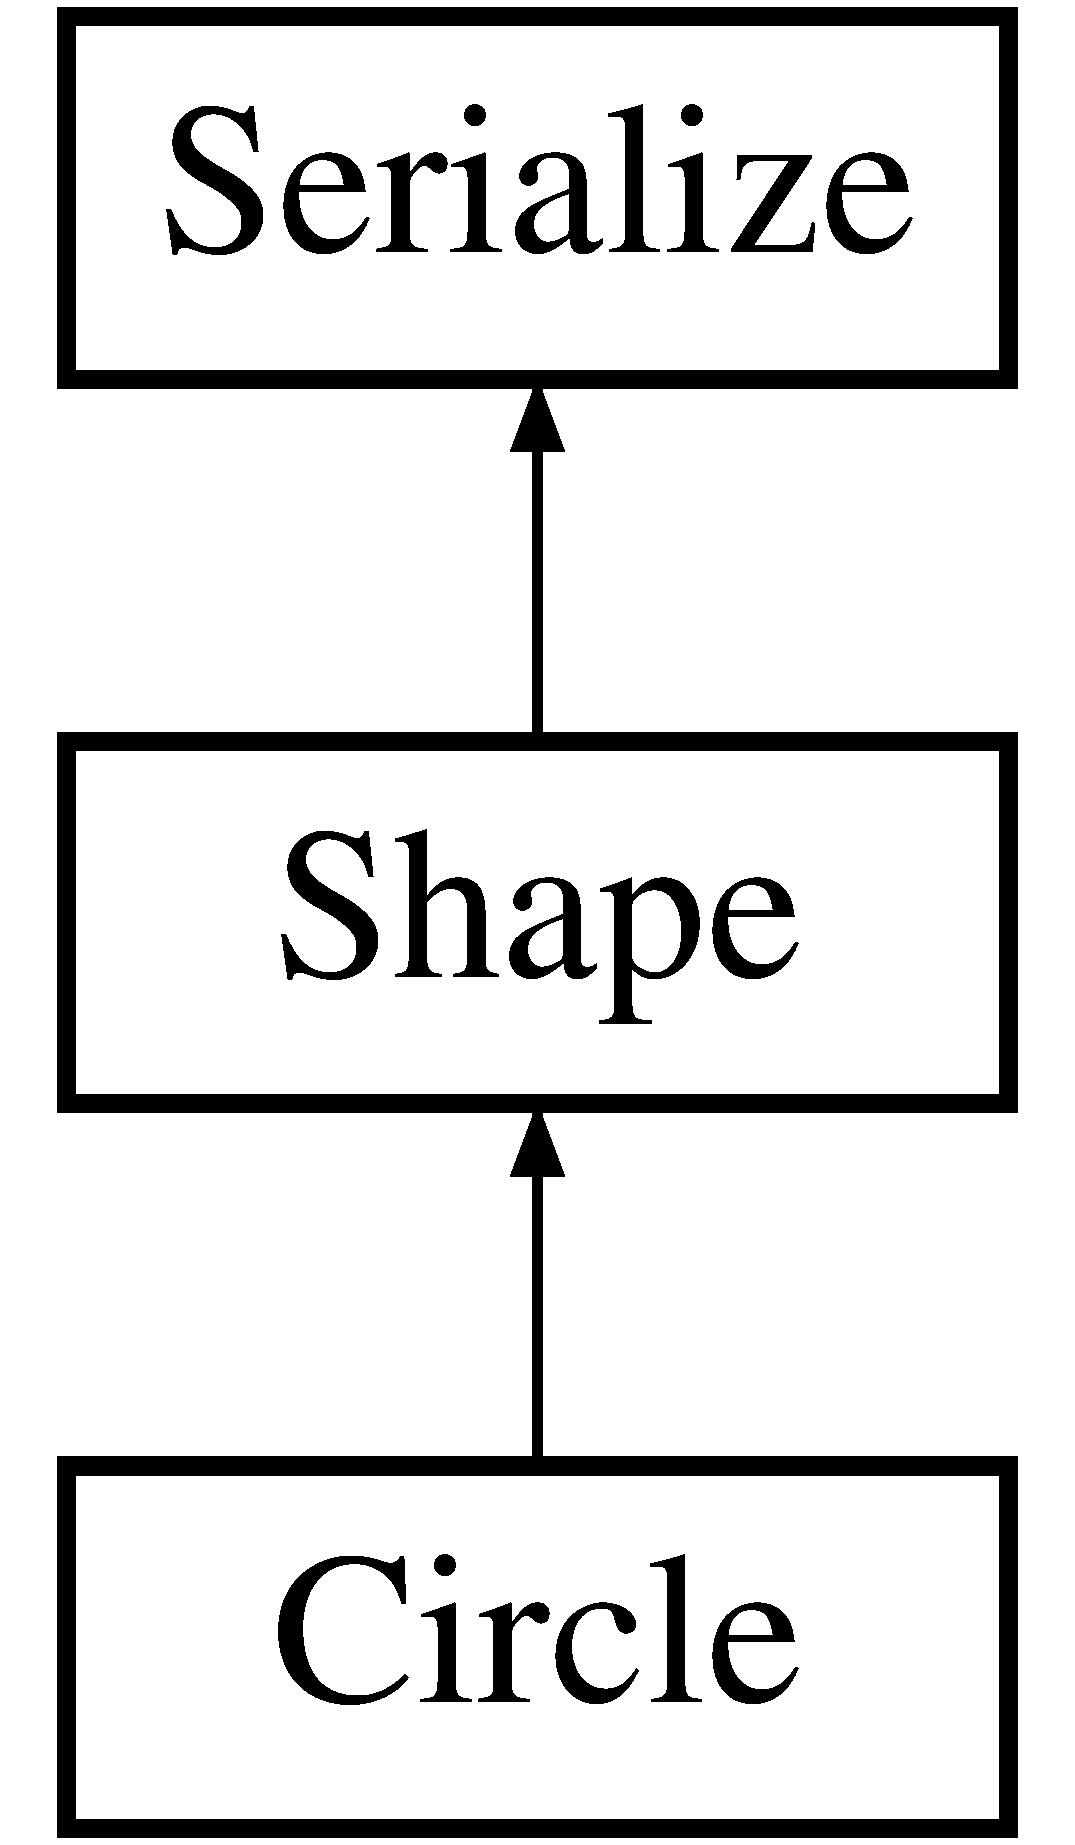
\includegraphics[height=3.000000cm]{classCircle}
\end{center}
\end{figure}
\subsection*{Public Member Functions}
\begin{DoxyCompactItemize}
\item 
\hyperlink{classCircle_a6dd3d6a0a6609e275dc16b7687244405}{Circle} (float radius, int ns)
\item 
virtual \hyperlink{classCircle_ae3f30436e645d73e368e8ee55f8d1650}{$\sim$\-Circle} ()
\item 
virtual void \hyperlink{classCircle_a59dab91c7a95f18e8b888a874c17826f}{fill} (float $\ast$v)
\end{DoxyCompactItemize}
\subsection*{Private Attributes}
\begin{DoxyCompactItemize}
\item 
float \hyperlink{classCircle_acbb9f46cef6c9deba7aa4e704bdc774f}{m\-\_\-radius}
\end{DoxyCompactItemize}
\subsection*{Additional Inherited Members}


\subsection{Constructor \& Destructor Documentation}
\hypertarget{classCircle_a6dd3d6a0a6609e275dc16b7687244405}{\index{Circle@{Circle}!Circle@{Circle}}
\index{Circle@{Circle}!Circle@{Circle}}
\subsubsection[{Circle}]{\setlength{\rightskip}{0pt plus 5cm}Circle\-::\-Circle (
\begin{DoxyParamCaption}
\item[{float}]{radius, }
\item[{int}]{ns}
\end{DoxyParamCaption}
)}}\label{classCircle_a6dd3d6a0a6609e275dc16b7687244405}
\hypertarget{classCircle_ae3f30436e645d73e368e8ee55f8d1650}{\index{Circle@{Circle}!$\sim$\-Circle@{$\sim$\-Circle}}
\index{$\sim$\-Circle@{$\sim$\-Circle}!Circle@{Circle}}
\subsubsection[{$\sim$\-Circle}]{\setlength{\rightskip}{0pt plus 5cm}Circle\-::$\sim$\-Circle (
\begin{DoxyParamCaption}
{}
\end{DoxyParamCaption}
)\hspace{0.3cm}{\ttfamily [virtual]}}}\label{classCircle_ae3f30436e645d73e368e8ee55f8d1650}


\subsection{Member Function Documentation}
\hypertarget{classCircle_a59dab91c7a95f18e8b888a874c17826f}{\index{Circle@{Circle}!fill@{fill}}
\index{fill@{fill}!Circle@{Circle}}
\subsubsection[{fill}]{\setlength{\rightskip}{0pt plus 5cm}void Circle\-::fill (
\begin{DoxyParamCaption}
\item[{float $\ast$}]{v}
\end{DoxyParamCaption}
)\hspace{0.3cm}{\ttfamily [virtual]}}}\label{classCircle_a59dab91c7a95f18e8b888a874c17826f}


Reimplemented from \hyperlink{classShape_a33be64d8e24518084b1c8f974f808387}{Shape}.



\subsection{Member Data Documentation}
\hypertarget{classCircle_acbb9f46cef6c9deba7aa4e704bdc774f}{\index{Circle@{Circle}!m\-\_\-radius@{m\-\_\-radius}}
\index{m\-\_\-radius@{m\-\_\-radius}!Circle@{Circle}}
\subsubsection[{m\-\_\-radius}]{\setlength{\rightskip}{0pt plus 5cm}float Circle\-::m\-\_\-radius\hspace{0.3cm}{\ttfamily [private]}}}\label{classCircle_acbb9f46cef6c9deba7aa4e704bdc774f}


The documentation for this class was generated from the following files\-:\begin{DoxyCompactItemize}
\item 
/home/ruijan/sw/bmi5/bmi5/include/\-Shape/\hyperlink{circle_8h}{circle.\-h}\item 
/home/ruijan/sw/bmi5/bmi5/src/\-Shape/\hyperlink{circle_8cpp}{circle.\-cpp}\end{DoxyCompactItemize}

\hypertarget{classDisplayText}{\section{Display\-Text Class Reference}
\label{classDisplayText}\index{Display\-Text@{Display\-Text}}
}


{\ttfamily \#include $<$display\-Text.\-h$>$}

Inheritance diagram for Display\-Text\-:\begin{figure}[H]
\begin{center}
\leavevmode
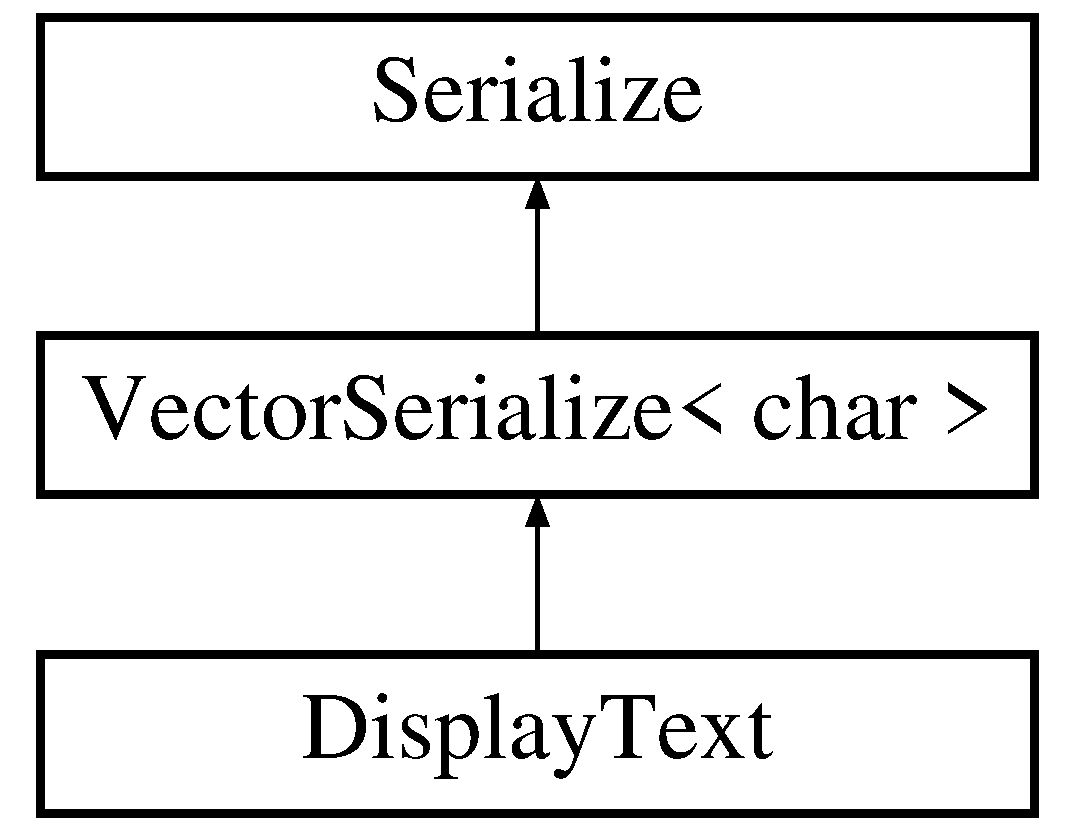
\includegraphics[height=3.000000cm]{classDisplayText}
\end{center}
\end{figure}
\subsection*{Public Member Functions}
\begin{DoxyCompactItemize}
\item 
\hyperlink{classDisplayText_a998e42cd6bab6ab04556b50f89b5209b}{Display\-Text} (int size)
\item 
\hyperlink{classDisplayText_a67c96d3dc8538032470131d4988b42bb}{$\sim$\-Display\-Text} ()
\item 
virtual bool \hyperlink{classDisplayText_a16d096c25b729eabfce141eb7dcf9012}{store} ()
\item 
virtual void \hyperlink{classDisplayText_a0c7a7a5200482ea4817f6c550dc7dea9}{clear} ()
\item 
virtual string \hyperlink{classDisplayText_af663118f6d5010d2d1d45f2bf3680dfc}{store\-Name} (int indx)
\item 
virtual int \hyperlink{classDisplayText_aaa8ccb67b152d79505e5acc8448770ed}{get\-Store\-Class} (int indx)
\item 
virtual void \hyperlink{classDisplayText_a81a37dd4e0fa54265843db620c371d02}{get\-Store\-Dims} (int indx, size\-\_\-t $\ast$dims)
\item 
virtual void $\ast$ \hyperlink{classDisplayText_aea5003c9c461955ec3c9a3a4b4fc2c25}{get\-Store} (int indx, int i)
\item 
virtual int \hyperlink{classDisplayText_a06b49281616900153577f7c731e4bd62}{num\-Stores} ()
\item 
virtual double $\ast$ \hyperlink{classDisplayText_ae5f08045997631736d8400ad3662fe5b}{mmap\-Read} (double $\ast$d)
\item 
virtual void \hyperlink{classDisplayText_a1eddd0c9f33244eb10540c51aa1dbfda}{draw} (int display, float ar)
\end{DoxyCompactItemize}
\subsection*{Public Attributes}
\begin{DoxyCompactItemize}
\item 
string \hyperlink{classDisplayText_a932a5d5bfd33d578faddb55ff098f180}{m\-\_\-text}
\item 
char \hyperlink{classDisplayText_a886201e135220482b8507be2b671544b}{m\-\_\-draw}
\item 
array$<$ float, 2 $>$ \hyperlink{classDisplayText_ae67cf19d70a36dac532b1a57daac904b}{m\-\_\-pos}
\item 
vector$<$ char $>$ \hyperlink{classDisplayText_a0f43c42a360464b92fbc9a1b5a2405d4}{v\-\_\-draw}
\item 
array$<$ unsigned char, 4 $>$ \hyperlink{classDisplayText_a680e8fb0a1dbd15c0fc9b60106f8a377}{m\-\_\-color}
\item 
vector$<$ array$<$ float, 2 $>$ $>$ \hyperlink{classDisplayText_a61592bbfe955f9bbe59390ba7f6581bc}{v\-\_\-pos}
\item 
vector$<$ array$<$ unsigned char, 4 $>$ $>$ \hyperlink{classDisplayText_af6d153a33c304bb21445e62ca402f72f}{v\-\_\-color}
\end{DoxyCompactItemize}


\subsection{Constructor \& Destructor Documentation}
\hypertarget{classDisplayText_a998e42cd6bab6ab04556b50f89b5209b}{\index{Display\-Text@{Display\-Text}!Display\-Text@{Display\-Text}}
\index{Display\-Text@{Display\-Text}!DisplayText@{Display\-Text}}
\subsubsection[{Display\-Text}]{\setlength{\rightskip}{0pt plus 5cm}Display\-Text\-::\-Display\-Text (
\begin{DoxyParamCaption}
\item[{int}]{size}
\end{DoxyParamCaption}
)}}\label{classDisplayText_a998e42cd6bab6ab04556b50f89b5209b}
\hypertarget{classDisplayText_a67c96d3dc8538032470131d4988b42bb}{\index{Display\-Text@{Display\-Text}!$\sim$\-Display\-Text@{$\sim$\-Display\-Text}}
\index{$\sim$\-Display\-Text@{$\sim$\-Display\-Text}!DisplayText@{Display\-Text}}
\subsubsection[{$\sim$\-Display\-Text}]{\setlength{\rightskip}{0pt plus 5cm}Display\-Text\-::$\sim$\-Display\-Text (
\begin{DoxyParamCaption}
{}
\end{DoxyParamCaption}
)}}\label{classDisplayText_a67c96d3dc8538032470131d4988b42bb}


\subsection{Member Function Documentation}
\hypertarget{classDisplayText_a0c7a7a5200482ea4817f6c550dc7dea9}{\index{Display\-Text@{Display\-Text}!clear@{clear}}
\index{clear@{clear}!DisplayText@{Display\-Text}}
\subsubsection[{clear}]{\setlength{\rightskip}{0pt plus 5cm}void Display\-Text\-::clear (
\begin{DoxyParamCaption}
{}
\end{DoxyParamCaption}
)\hspace{0.3cm}{\ttfamily [virtual]}}}\label{classDisplayText_a0c7a7a5200482ea4817f6c550dc7dea9}


Reimplemented from \hyperlink{classVectorSerialize_ae94606fef7aec9ade8142d3cd56449ab}{Vector\-Serialize$<$ char $>$}.

\hypertarget{classDisplayText_a1eddd0c9f33244eb10540c51aa1dbfda}{\index{Display\-Text@{Display\-Text}!draw@{draw}}
\index{draw@{draw}!DisplayText@{Display\-Text}}
\subsubsection[{draw}]{\setlength{\rightskip}{0pt plus 5cm}void Display\-Text\-::draw (
\begin{DoxyParamCaption}
\item[{int}]{display, }
\item[{float}]{ar}
\end{DoxyParamCaption}
)\hspace{0.3cm}{\ttfamily [virtual]}}}\label{classDisplayText_a1eddd0c9f33244eb10540c51aa1dbfda}


Reimplemented from \hyperlink{classSerialize_a0cf1d14e41052c6eabe53c90a37c227b}{Serialize}.

\hypertarget{classDisplayText_aea5003c9c461955ec3c9a3a4b4fc2c25}{\index{Display\-Text@{Display\-Text}!get\-Store@{get\-Store}}
\index{get\-Store@{get\-Store}!DisplayText@{Display\-Text}}
\subsubsection[{get\-Store}]{\setlength{\rightskip}{0pt plus 5cm}void $\ast$ Display\-Text\-::get\-Store (
\begin{DoxyParamCaption}
\item[{int}]{indx, }
\item[{int}]{i}
\end{DoxyParamCaption}
)\hspace{0.3cm}{\ttfamily [virtual]}}}\label{classDisplayText_aea5003c9c461955ec3c9a3a4b4fc2c25}


Reimplemented from \hyperlink{classVectorSerialize_a08f1412b11fb7b034da21c5ec131489b}{Vector\-Serialize$<$ char $>$}.

\hypertarget{classDisplayText_aaa8ccb67b152d79505e5acc8448770ed}{\index{Display\-Text@{Display\-Text}!get\-Store\-Class@{get\-Store\-Class}}
\index{get\-Store\-Class@{get\-Store\-Class}!DisplayText@{Display\-Text}}
\subsubsection[{get\-Store\-Class}]{\setlength{\rightskip}{0pt plus 5cm}int Display\-Text\-::get\-Store\-Class (
\begin{DoxyParamCaption}
\item[{int}]{indx}
\end{DoxyParamCaption}
)\hspace{0.3cm}{\ttfamily [virtual]}}}\label{classDisplayText_aaa8ccb67b152d79505e5acc8448770ed}


Reimplemented from \hyperlink{classVectorSerialize_a03d8454fff77942e63cd1764f1013f2d}{Vector\-Serialize$<$ char $>$}.

\hypertarget{classDisplayText_a81a37dd4e0fa54265843db620c371d02}{\index{Display\-Text@{Display\-Text}!get\-Store\-Dims@{get\-Store\-Dims}}
\index{get\-Store\-Dims@{get\-Store\-Dims}!DisplayText@{Display\-Text}}
\subsubsection[{get\-Store\-Dims}]{\setlength{\rightskip}{0pt plus 5cm}void Display\-Text\-::get\-Store\-Dims (
\begin{DoxyParamCaption}
\item[{int}]{indx, }
\item[{size\-\_\-t $\ast$}]{dims}
\end{DoxyParamCaption}
)\hspace{0.3cm}{\ttfamily [virtual]}}}\label{classDisplayText_a81a37dd4e0fa54265843db620c371d02}


Reimplemented from \hyperlink{classVectorSerialize_aa22f90d57d8802670716f4b859d6b069}{Vector\-Serialize$<$ char $>$}.

\hypertarget{classDisplayText_ae5f08045997631736d8400ad3662fe5b}{\index{Display\-Text@{Display\-Text}!mmap\-Read@{mmap\-Read}}
\index{mmap\-Read@{mmap\-Read}!DisplayText@{Display\-Text}}
\subsubsection[{mmap\-Read}]{\setlength{\rightskip}{0pt plus 5cm}double $\ast$ Display\-Text\-::mmap\-Read (
\begin{DoxyParamCaption}
\item[{double $\ast$}]{d}
\end{DoxyParamCaption}
)\hspace{0.3cm}{\ttfamily [virtual]}}}\label{classDisplayText_ae5f08045997631736d8400ad3662fe5b}


Reimplemented from \hyperlink{classVectorSerialize_a087c30b15095d1b230705e42123eb3db}{Vector\-Serialize$<$ char $>$}.

\hypertarget{classDisplayText_a06b49281616900153577f7c731e4bd62}{\index{Display\-Text@{Display\-Text}!num\-Stores@{num\-Stores}}
\index{num\-Stores@{num\-Stores}!DisplayText@{Display\-Text}}
\subsubsection[{num\-Stores}]{\setlength{\rightskip}{0pt plus 5cm}int Display\-Text\-::num\-Stores (
\begin{DoxyParamCaption}
{}
\end{DoxyParamCaption}
)\hspace{0.3cm}{\ttfamily [virtual]}}}\label{classDisplayText_a06b49281616900153577f7c731e4bd62}


Reimplemented from \hyperlink{classVectorSerialize_a15226c69bda0fff870f20026f8681d80}{Vector\-Serialize$<$ char $>$}.

\hypertarget{classDisplayText_a16d096c25b729eabfce141eb7dcf9012}{\index{Display\-Text@{Display\-Text}!store@{store}}
\index{store@{store}!DisplayText@{Display\-Text}}
\subsubsection[{store}]{\setlength{\rightskip}{0pt plus 5cm}bool Display\-Text\-::store (
\begin{DoxyParamCaption}
{}
\end{DoxyParamCaption}
)\hspace{0.3cm}{\ttfamily [virtual]}}}\label{classDisplayText_a16d096c25b729eabfce141eb7dcf9012}


Reimplemented from \hyperlink{classVectorSerialize_afd6b6dc8768969dae5f27f46eeab83e6}{Vector\-Serialize$<$ char $>$}.

\hypertarget{classDisplayText_af663118f6d5010d2d1d45f2bf3680dfc}{\index{Display\-Text@{Display\-Text}!store\-Name@{store\-Name}}
\index{store\-Name@{store\-Name}!DisplayText@{Display\-Text}}
\subsubsection[{store\-Name}]{\setlength{\rightskip}{0pt plus 5cm}string Display\-Text\-::store\-Name (
\begin{DoxyParamCaption}
\item[{int}]{indx}
\end{DoxyParamCaption}
)\hspace{0.3cm}{\ttfamily [virtual]}}}\label{classDisplayText_af663118f6d5010d2d1d45f2bf3680dfc}


Reimplemented from \hyperlink{classVectorSerialize_a929f94f68d0a99c61308520a679ae1a2}{Vector\-Serialize$<$ char $>$}.



\subsection{Member Data Documentation}
\hypertarget{classDisplayText_a680e8fb0a1dbd15c0fc9b60106f8a377}{\index{Display\-Text@{Display\-Text}!m\-\_\-color@{m\-\_\-color}}
\index{m\-\_\-color@{m\-\_\-color}!DisplayText@{Display\-Text}}
\subsubsection[{m\-\_\-color}]{\setlength{\rightskip}{0pt plus 5cm}array$<$unsigned char,4$>$ Display\-Text\-::m\-\_\-color}}\label{classDisplayText_a680e8fb0a1dbd15c0fc9b60106f8a377}
\hypertarget{classDisplayText_a886201e135220482b8507be2b671544b}{\index{Display\-Text@{Display\-Text}!m\-\_\-draw@{m\-\_\-draw}}
\index{m\-\_\-draw@{m\-\_\-draw}!DisplayText@{Display\-Text}}
\subsubsection[{m\-\_\-draw}]{\setlength{\rightskip}{0pt plus 5cm}char Display\-Text\-::m\-\_\-draw}}\label{classDisplayText_a886201e135220482b8507be2b671544b}
\hypertarget{classDisplayText_ae67cf19d70a36dac532b1a57daac904b}{\index{Display\-Text@{Display\-Text}!m\-\_\-pos@{m\-\_\-pos}}
\index{m\-\_\-pos@{m\-\_\-pos}!DisplayText@{Display\-Text}}
\subsubsection[{m\-\_\-pos}]{\setlength{\rightskip}{0pt plus 5cm}array$<$float,2$>$ Display\-Text\-::m\-\_\-pos}}\label{classDisplayText_ae67cf19d70a36dac532b1a57daac904b}
\hypertarget{classDisplayText_a932a5d5bfd33d578faddb55ff098f180}{\index{Display\-Text@{Display\-Text}!m\-\_\-text@{m\-\_\-text}}
\index{m\-\_\-text@{m\-\_\-text}!DisplayText@{Display\-Text}}
\subsubsection[{m\-\_\-text}]{\setlength{\rightskip}{0pt plus 5cm}string Display\-Text\-::m\-\_\-text}}\label{classDisplayText_a932a5d5bfd33d578faddb55ff098f180}
\hypertarget{classDisplayText_af6d153a33c304bb21445e62ca402f72f}{\index{Display\-Text@{Display\-Text}!v\-\_\-color@{v\-\_\-color}}
\index{v\-\_\-color@{v\-\_\-color}!DisplayText@{Display\-Text}}
\subsubsection[{v\-\_\-color}]{\setlength{\rightskip}{0pt plus 5cm}vector$<$array$<$unsigned char,4$>$ $>$ Display\-Text\-::v\-\_\-color}}\label{classDisplayText_af6d153a33c304bb21445e62ca402f72f}
\hypertarget{classDisplayText_a0f43c42a360464b92fbc9a1b5a2405d4}{\index{Display\-Text@{Display\-Text}!v\-\_\-draw@{v\-\_\-draw}}
\index{v\-\_\-draw@{v\-\_\-draw}!DisplayText@{Display\-Text}}
\subsubsection[{v\-\_\-draw}]{\setlength{\rightskip}{0pt plus 5cm}vector$<$char$>$ Display\-Text\-::v\-\_\-draw}}\label{classDisplayText_a0f43c42a360464b92fbc9a1b5a2405d4}
\hypertarget{classDisplayText_a61592bbfe955f9bbe59390ba7f6581bc}{\index{Display\-Text@{Display\-Text}!v\-\_\-pos@{v\-\_\-pos}}
\index{v\-\_\-pos@{v\-\_\-pos}!DisplayText@{Display\-Text}}
\subsubsection[{v\-\_\-pos}]{\setlength{\rightskip}{0pt plus 5cm}vector$<$array$<$float,2$>$ $>$ Display\-Text\-::v\-\_\-pos}}\label{classDisplayText_a61592bbfe955f9bbe59390ba7f6581bc}


The documentation for this class was generated from the following files\-:\begin{DoxyCompactItemize}
\item 
/home/ruijan/sw/bmi5/bmi5/include/\-Shape/\hyperlink{displayText_8h}{display\-Text.\-h}\item 
/home/ruijan/sw/bmi5/bmi5/src/\-Shape/\hyperlink{displayText_8cpp}{display\-Text.\-cpp}\end{DoxyCompactItemize}

\hypertarget{classFrameSerialize}{\section{Frame\-Serialize Class Reference}
\label{classFrameSerialize}\index{Frame\-Serialize@{Frame\-Serialize}}
}


{\ttfamily \#include $<$frame\-Serialize.\-h$>$}

Inheritance diagram for Frame\-Serialize\-:\begin{figure}[H]
\begin{center}
\leavevmode
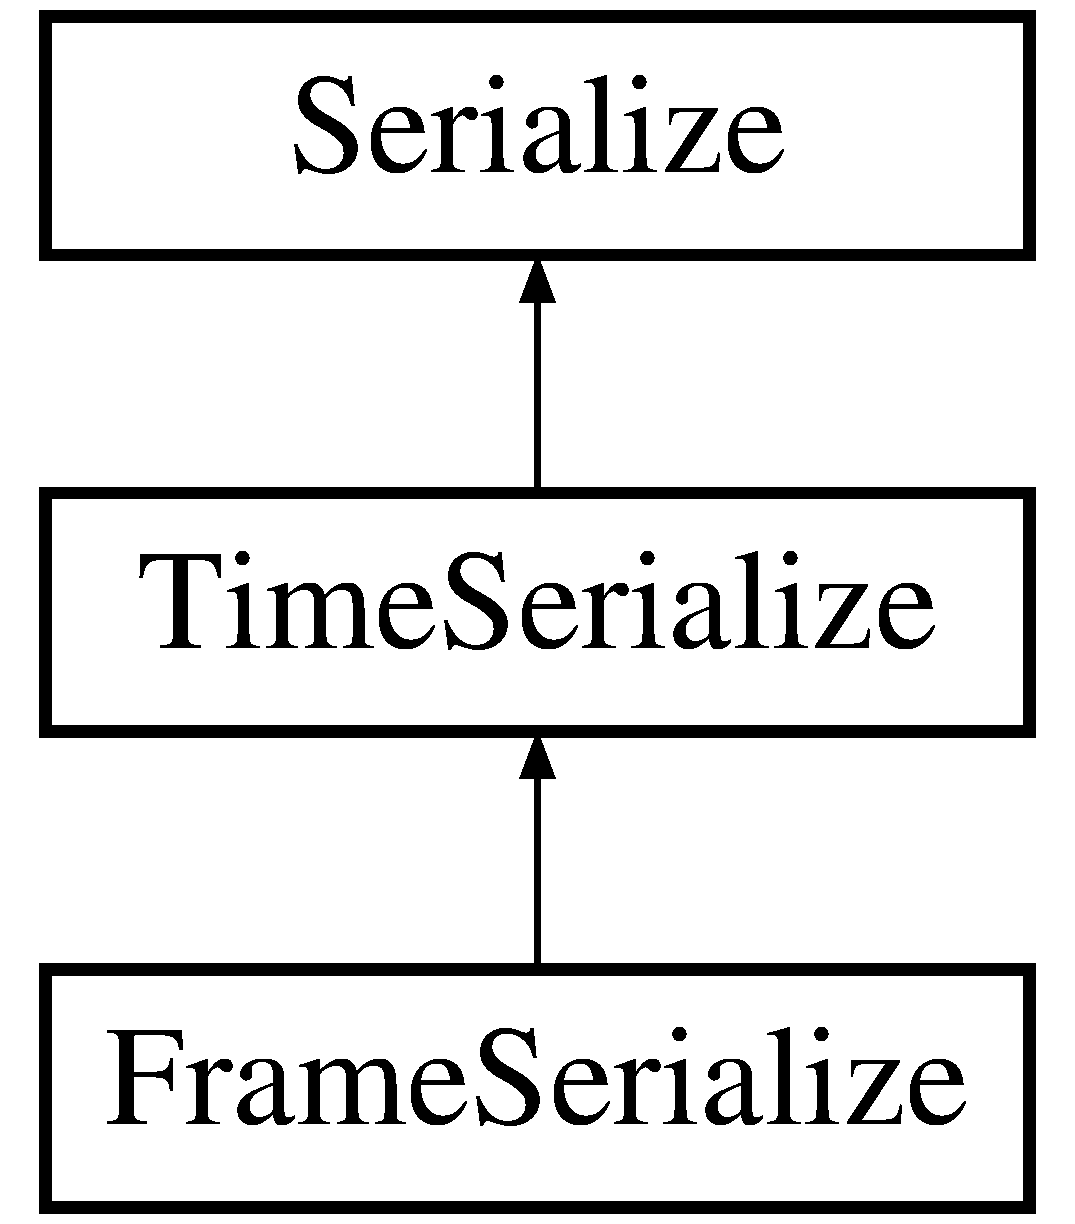
\includegraphics[height=3.000000cm]{classFrameSerialize}
\end{center}
\end{figure}
\subsection*{Public Member Functions}
\begin{DoxyCompactItemize}
\item 
\hyperlink{classFrameSerialize_a9f0dd912a61be08b54b1d8b5ba5c7f8b}{Frame\-Serialize} ()
\item 
\hyperlink{classFrameSerialize_af457bbe269ca51a7ee49514929b0e9e5}{$\sim$\-Frame\-Serialize} ()
\item 
virtual bool \hyperlink{classFrameSerialize_a5c2bbf78b071f73554611b82ad395573}{store} ()
\item 
virtual bool \hyperlink{classFrameSerialize_aa687bac3fbff650d93d45be0ad83de5f}{store} (int frame)
\item 
virtual double $\ast$ \hyperlink{classFrameSerialize_a9d775f9c379f0444a82cd309bba9e9b1}{mmap\-Read} (double $\ast$d)
\end{DoxyCompactItemize}
\subsection*{Public Attributes}
\begin{DoxyCompactItemize}
\item 
double \hyperlink{classFrameSerialize_a0be80383beb183887e34850ef542be32}{m\-\_\-time}
\item 
double \hyperlink{classFrameSerialize_a3299fc53239b5e9d4c1c6441be8c5a00}{m\-\_\-ticks}
\item 
int \hyperlink{classFrameSerialize_a6cf05a591ccdbea37fda4192e51b18cf}{m\-\_\-frame}
\end{DoxyCompactItemize}


\subsection{Constructor \& Destructor Documentation}
\hypertarget{classFrameSerialize_a9f0dd912a61be08b54b1d8b5ba5c7f8b}{\index{Frame\-Serialize@{Frame\-Serialize}!Frame\-Serialize@{Frame\-Serialize}}
\index{Frame\-Serialize@{Frame\-Serialize}!FrameSerialize@{Frame\-Serialize}}
\subsubsection[{Frame\-Serialize}]{\setlength{\rightskip}{0pt plus 5cm}Frame\-Serialize\-::\-Frame\-Serialize (
\begin{DoxyParamCaption}
{}
\end{DoxyParamCaption}
)}}\label{classFrameSerialize_a9f0dd912a61be08b54b1d8b5ba5c7f8b}
\hypertarget{classFrameSerialize_af457bbe269ca51a7ee49514929b0e9e5}{\index{Frame\-Serialize@{Frame\-Serialize}!$\sim$\-Frame\-Serialize@{$\sim$\-Frame\-Serialize}}
\index{$\sim$\-Frame\-Serialize@{$\sim$\-Frame\-Serialize}!FrameSerialize@{Frame\-Serialize}}
\subsubsection[{$\sim$\-Frame\-Serialize}]{\setlength{\rightskip}{0pt plus 5cm}Frame\-Serialize\-::$\sim$\-Frame\-Serialize (
\begin{DoxyParamCaption}
{}
\end{DoxyParamCaption}
)}}\label{classFrameSerialize_af457bbe269ca51a7ee49514929b0e9e5}


\subsection{Member Function Documentation}
\hypertarget{classFrameSerialize_a9d775f9c379f0444a82cd309bba9e9b1}{\index{Frame\-Serialize@{Frame\-Serialize}!mmap\-Read@{mmap\-Read}}
\index{mmap\-Read@{mmap\-Read}!FrameSerialize@{Frame\-Serialize}}
\subsubsection[{mmap\-Read}]{\setlength{\rightskip}{0pt plus 5cm}double $\ast$ Frame\-Serialize\-::mmap\-Read (
\begin{DoxyParamCaption}
\item[{double $\ast$}]{d}
\end{DoxyParamCaption}
)\hspace{0.3cm}{\ttfamily [virtual]}}}\label{classFrameSerialize_a9d775f9c379f0444a82cd309bba9e9b1}


Reimplemented from \hyperlink{classTimeSerialize_ac7a17bf484eb4e7970532b6a1ed65325}{Time\-Serialize}.

\hypertarget{classFrameSerialize_a5c2bbf78b071f73554611b82ad395573}{\index{Frame\-Serialize@{Frame\-Serialize}!store@{store}}
\index{store@{store}!FrameSerialize@{Frame\-Serialize}}
\subsubsection[{store}]{\setlength{\rightskip}{0pt plus 5cm}bool Frame\-Serialize\-::store (
\begin{DoxyParamCaption}
{}
\end{DoxyParamCaption}
)\hspace{0.3cm}{\ttfamily [virtual]}}}\label{classFrameSerialize_a5c2bbf78b071f73554611b82ad395573}


Reimplemented from \hyperlink{classTimeSerialize_a5fa3f8491cf69cafb608ed06d16b744b}{Time\-Serialize}.

\hypertarget{classFrameSerialize_aa687bac3fbff650d93d45be0ad83de5f}{\index{Frame\-Serialize@{Frame\-Serialize}!store@{store}}
\index{store@{store}!FrameSerialize@{Frame\-Serialize}}
\subsubsection[{store}]{\setlength{\rightskip}{0pt plus 5cm}bool Frame\-Serialize\-::store (
\begin{DoxyParamCaption}
\item[{int}]{frame}
\end{DoxyParamCaption}
)\hspace{0.3cm}{\ttfamily [virtual]}}}\label{classFrameSerialize_aa687bac3fbff650d93d45be0ad83de5f}


\subsection{Member Data Documentation}
\hypertarget{classFrameSerialize_a6cf05a591ccdbea37fda4192e51b18cf}{\index{Frame\-Serialize@{Frame\-Serialize}!m\-\_\-frame@{m\-\_\-frame}}
\index{m\-\_\-frame@{m\-\_\-frame}!FrameSerialize@{Frame\-Serialize}}
\subsubsection[{m\-\_\-frame}]{\setlength{\rightskip}{0pt plus 5cm}int Frame\-Serialize\-::m\-\_\-frame}}\label{classFrameSerialize_a6cf05a591ccdbea37fda4192e51b18cf}
\hypertarget{classFrameSerialize_a3299fc53239b5e9d4c1c6441be8c5a00}{\index{Frame\-Serialize@{Frame\-Serialize}!m\-\_\-ticks@{m\-\_\-ticks}}
\index{m\-\_\-ticks@{m\-\_\-ticks}!FrameSerialize@{Frame\-Serialize}}
\subsubsection[{m\-\_\-ticks}]{\setlength{\rightskip}{0pt plus 5cm}double Frame\-Serialize\-::m\-\_\-ticks}}\label{classFrameSerialize_a3299fc53239b5e9d4c1c6441be8c5a00}
\hypertarget{classFrameSerialize_a0be80383beb183887e34850ef542be32}{\index{Frame\-Serialize@{Frame\-Serialize}!m\-\_\-time@{m\-\_\-time}}
\index{m\-\_\-time@{m\-\_\-time}!FrameSerialize@{Frame\-Serialize}}
\subsubsection[{m\-\_\-time}]{\setlength{\rightskip}{0pt plus 5cm}double Frame\-Serialize\-::m\-\_\-time}}\label{classFrameSerialize_a0be80383beb183887e34850ef542be32}


The documentation for this class was generated from the following files\-:\begin{DoxyCompactItemize}
\item 
/home/ruijan/sw/bmi5/bmi5/include/\-Serialize/\hyperlink{frameSerialize_8h}{frame\-Serialize.\-h}\item 
/home/ruijan/sw/bmi5/bmi5/src/\-Serialize/\hyperlink{frameSerialize_8cpp}{frame\-Serialize.\-cpp}\end{DoxyCompactItemize}

\hypertarget{structglInfo}{\section{gl\-Info Struct Reference}
\label{structglInfo}\index{gl\-Info@{gl\-Info}}
}


{\ttfamily \#include $<$gl\-Info.\-h$>$}

\subsection*{Public Member Functions}
\begin{DoxyCompactItemize}
\item 
\hyperlink{structglInfo_a0e1a3233ed1bf13d40e2392358bd9179}{gl\-Info} ()
\item 
bool \hyperlink{structglInfo_a15576e01d26b015a1e1e9fb71437c101}{get\-Info} ()
\item 
void \hyperlink{structglInfo_aea08606b991de4d4975dd14e9bcd1a0c}{print\-Self} ()
\item 
bool \hyperlink{structglInfo_afb450582bfc8d67eb3714a785b104602}{is\-Extension\-Supported} (const std\-::string \&ext)
\end{DoxyCompactItemize}
\subsection*{Public Attributes}
\begin{DoxyCompactItemize}
\item 
std\-::string \hyperlink{structglInfo_a8d6952c9ef0c2f4d7311f448482509af}{vendor}
\item 
std\-::string \hyperlink{structglInfo_ad6eee9cd07b1c1d39bce1294bbf4f025}{renderer}
\item 
std\-::string \hyperlink{structglInfo_a3c189d62cff793f67c7df3d4d1992eda}{version}
\item 
std\-::vector$<$ std\-::string $>$ \hyperlink{structglInfo_acf0baeef3c59256b5421e7f3a02f5e89}{extensions}
\item 
int \hyperlink{structglInfo_a8ca02246f86e2c1872772e468fa7b510}{red\-Bits}
\item 
int \hyperlink{structglInfo_aac9180e543cb14496c2ee225268e4d70}{green\-Bits}
\item 
int \hyperlink{structglInfo_ab297321b61208d90c5e929a39462f7f2}{blue\-Bits}
\item 
int \hyperlink{structglInfo_ac1f6ab1145051cb46ecf0716c0d5a453}{alpha\-Bits}
\item 
int \hyperlink{structglInfo_a7c10c7ae71e40d05e16dd29d5402505e}{depth\-Bits}
\item 
int \hyperlink{structglInfo_ae845cb4ded351fd5d12435220e6e185d}{stencil\-Bits}
\item 
int \hyperlink{structglInfo_afbde9a0fb66cc337cc0b1e5b48c2562d}{max\-Texture\-Size}
\item 
int \hyperlink{structglInfo_a8ca045798dcecb9331233410575a2648}{max\-Lights}
\item 
int \hyperlink{structglInfo_a2032498ee944c2e0d18395d54736aaee}{max\-Attrib\-Stacks}
\item 
int \hyperlink{structglInfo_a8fe530a903dc0e940d411088ca3babc2}{max\-Model\-View\-Stacks}
\item 
int \hyperlink{structglInfo_a1c2c13828297dc283a16ce0c1d15a137}{max\-Projection\-Stacks}
\item 
int \hyperlink{structglInfo_a0de92684a9e00e09d64137f2d86f472d}{max\-Clip\-Planes}
\item 
int \hyperlink{structglInfo_a6b9e47f0d7b9237b607bb6dad38527fb}{max\-Texture\-Stacks}
\end{DoxyCompactItemize}


\subsection{Constructor \& Destructor Documentation}
\hypertarget{structglInfo_a0e1a3233ed1bf13d40e2392358bd9179}{\index{gl\-Info@{gl\-Info}!gl\-Info@{gl\-Info}}
\index{gl\-Info@{gl\-Info}!glInfo@{gl\-Info}}
\subsubsection[{gl\-Info}]{\setlength{\rightskip}{0pt plus 5cm}gl\-Info\-::gl\-Info (
\begin{DoxyParamCaption}
{}
\end{DoxyParamCaption}
)\hspace{0.3cm}{\ttfamily [inline]}}}\label{structglInfo_a0e1a3233ed1bf13d40e2392358bd9179}


\subsection{Member Function Documentation}
\hypertarget{structglInfo_a15576e01d26b015a1e1e9fb71437c101}{\index{gl\-Info@{gl\-Info}!get\-Info@{get\-Info}}
\index{get\-Info@{get\-Info}!glInfo@{gl\-Info}}
\subsubsection[{get\-Info}]{\setlength{\rightskip}{0pt plus 5cm}bool gl\-Info\-::get\-Info (
\begin{DoxyParamCaption}
{}
\end{DoxyParamCaption}
)}}\label{structglInfo_a15576e01d26b015a1e1e9fb71437c101}
\hypertarget{structglInfo_afb450582bfc8d67eb3714a785b104602}{\index{gl\-Info@{gl\-Info}!is\-Extension\-Supported@{is\-Extension\-Supported}}
\index{is\-Extension\-Supported@{is\-Extension\-Supported}!glInfo@{gl\-Info}}
\subsubsection[{is\-Extension\-Supported}]{\setlength{\rightskip}{0pt plus 5cm}bool gl\-Info\-::is\-Extension\-Supported (
\begin{DoxyParamCaption}
\item[{const std\-::string \&}]{ext}
\end{DoxyParamCaption}
)}}\label{structglInfo_afb450582bfc8d67eb3714a785b104602}
\hypertarget{structglInfo_aea08606b991de4d4975dd14e9bcd1a0c}{\index{gl\-Info@{gl\-Info}!print\-Self@{print\-Self}}
\index{print\-Self@{print\-Self}!glInfo@{gl\-Info}}
\subsubsection[{print\-Self}]{\setlength{\rightskip}{0pt plus 5cm}void gl\-Info\-::print\-Self (
\begin{DoxyParamCaption}
{}
\end{DoxyParamCaption}
)}}\label{structglInfo_aea08606b991de4d4975dd14e9bcd1a0c}


\subsection{Member Data Documentation}
\hypertarget{structglInfo_ac1f6ab1145051cb46ecf0716c0d5a453}{\index{gl\-Info@{gl\-Info}!alpha\-Bits@{alpha\-Bits}}
\index{alpha\-Bits@{alpha\-Bits}!glInfo@{gl\-Info}}
\subsubsection[{alpha\-Bits}]{\setlength{\rightskip}{0pt plus 5cm}int gl\-Info\-::alpha\-Bits}}\label{structglInfo_ac1f6ab1145051cb46ecf0716c0d5a453}
\hypertarget{structglInfo_ab297321b61208d90c5e929a39462f7f2}{\index{gl\-Info@{gl\-Info}!blue\-Bits@{blue\-Bits}}
\index{blue\-Bits@{blue\-Bits}!glInfo@{gl\-Info}}
\subsubsection[{blue\-Bits}]{\setlength{\rightskip}{0pt plus 5cm}int gl\-Info\-::blue\-Bits}}\label{structglInfo_ab297321b61208d90c5e929a39462f7f2}
\hypertarget{structglInfo_a7c10c7ae71e40d05e16dd29d5402505e}{\index{gl\-Info@{gl\-Info}!depth\-Bits@{depth\-Bits}}
\index{depth\-Bits@{depth\-Bits}!glInfo@{gl\-Info}}
\subsubsection[{depth\-Bits}]{\setlength{\rightskip}{0pt plus 5cm}int gl\-Info\-::depth\-Bits}}\label{structglInfo_a7c10c7ae71e40d05e16dd29d5402505e}
\hypertarget{structglInfo_acf0baeef3c59256b5421e7f3a02f5e89}{\index{gl\-Info@{gl\-Info}!extensions@{extensions}}
\index{extensions@{extensions}!glInfo@{gl\-Info}}
\subsubsection[{extensions}]{\setlength{\rightskip}{0pt plus 5cm}std\-::vector$<$std\-::string$>$ gl\-Info\-::extensions}}\label{structglInfo_acf0baeef3c59256b5421e7f3a02f5e89}
\hypertarget{structglInfo_aac9180e543cb14496c2ee225268e4d70}{\index{gl\-Info@{gl\-Info}!green\-Bits@{green\-Bits}}
\index{green\-Bits@{green\-Bits}!glInfo@{gl\-Info}}
\subsubsection[{green\-Bits}]{\setlength{\rightskip}{0pt plus 5cm}int gl\-Info\-::green\-Bits}}\label{structglInfo_aac9180e543cb14496c2ee225268e4d70}
\hypertarget{structglInfo_a2032498ee944c2e0d18395d54736aaee}{\index{gl\-Info@{gl\-Info}!max\-Attrib\-Stacks@{max\-Attrib\-Stacks}}
\index{max\-Attrib\-Stacks@{max\-Attrib\-Stacks}!glInfo@{gl\-Info}}
\subsubsection[{max\-Attrib\-Stacks}]{\setlength{\rightskip}{0pt plus 5cm}int gl\-Info\-::max\-Attrib\-Stacks}}\label{structglInfo_a2032498ee944c2e0d18395d54736aaee}
\hypertarget{structglInfo_a0de92684a9e00e09d64137f2d86f472d}{\index{gl\-Info@{gl\-Info}!max\-Clip\-Planes@{max\-Clip\-Planes}}
\index{max\-Clip\-Planes@{max\-Clip\-Planes}!glInfo@{gl\-Info}}
\subsubsection[{max\-Clip\-Planes}]{\setlength{\rightskip}{0pt plus 5cm}int gl\-Info\-::max\-Clip\-Planes}}\label{structglInfo_a0de92684a9e00e09d64137f2d86f472d}
\hypertarget{structglInfo_a8ca045798dcecb9331233410575a2648}{\index{gl\-Info@{gl\-Info}!max\-Lights@{max\-Lights}}
\index{max\-Lights@{max\-Lights}!glInfo@{gl\-Info}}
\subsubsection[{max\-Lights}]{\setlength{\rightskip}{0pt plus 5cm}int gl\-Info\-::max\-Lights}}\label{structglInfo_a8ca045798dcecb9331233410575a2648}
\hypertarget{structglInfo_a8fe530a903dc0e940d411088ca3babc2}{\index{gl\-Info@{gl\-Info}!max\-Model\-View\-Stacks@{max\-Model\-View\-Stacks}}
\index{max\-Model\-View\-Stacks@{max\-Model\-View\-Stacks}!glInfo@{gl\-Info}}
\subsubsection[{max\-Model\-View\-Stacks}]{\setlength{\rightskip}{0pt plus 5cm}int gl\-Info\-::max\-Model\-View\-Stacks}}\label{structglInfo_a8fe530a903dc0e940d411088ca3babc2}
\hypertarget{structglInfo_a1c2c13828297dc283a16ce0c1d15a137}{\index{gl\-Info@{gl\-Info}!max\-Projection\-Stacks@{max\-Projection\-Stacks}}
\index{max\-Projection\-Stacks@{max\-Projection\-Stacks}!glInfo@{gl\-Info}}
\subsubsection[{max\-Projection\-Stacks}]{\setlength{\rightskip}{0pt plus 5cm}int gl\-Info\-::max\-Projection\-Stacks}}\label{structglInfo_a1c2c13828297dc283a16ce0c1d15a137}
\hypertarget{structglInfo_afbde9a0fb66cc337cc0b1e5b48c2562d}{\index{gl\-Info@{gl\-Info}!max\-Texture\-Size@{max\-Texture\-Size}}
\index{max\-Texture\-Size@{max\-Texture\-Size}!glInfo@{gl\-Info}}
\subsubsection[{max\-Texture\-Size}]{\setlength{\rightskip}{0pt plus 5cm}int gl\-Info\-::max\-Texture\-Size}}\label{structglInfo_afbde9a0fb66cc337cc0b1e5b48c2562d}
\hypertarget{structglInfo_a6b9e47f0d7b9237b607bb6dad38527fb}{\index{gl\-Info@{gl\-Info}!max\-Texture\-Stacks@{max\-Texture\-Stacks}}
\index{max\-Texture\-Stacks@{max\-Texture\-Stacks}!glInfo@{gl\-Info}}
\subsubsection[{max\-Texture\-Stacks}]{\setlength{\rightskip}{0pt plus 5cm}int gl\-Info\-::max\-Texture\-Stacks}}\label{structglInfo_a6b9e47f0d7b9237b607bb6dad38527fb}
\hypertarget{structglInfo_a8ca02246f86e2c1872772e468fa7b510}{\index{gl\-Info@{gl\-Info}!red\-Bits@{red\-Bits}}
\index{red\-Bits@{red\-Bits}!glInfo@{gl\-Info}}
\subsubsection[{red\-Bits}]{\setlength{\rightskip}{0pt plus 5cm}int gl\-Info\-::red\-Bits}}\label{structglInfo_a8ca02246f86e2c1872772e468fa7b510}
\hypertarget{structglInfo_ad6eee9cd07b1c1d39bce1294bbf4f025}{\index{gl\-Info@{gl\-Info}!renderer@{renderer}}
\index{renderer@{renderer}!glInfo@{gl\-Info}}
\subsubsection[{renderer}]{\setlength{\rightskip}{0pt plus 5cm}std\-::string gl\-Info\-::renderer}}\label{structglInfo_ad6eee9cd07b1c1d39bce1294bbf4f025}
\hypertarget{structglInfo_ae845cb4ded351fd5d12435220e6e185d}{\index{gl\-Info@{gl\-Info}!stencil\-Bits@{stencil\-Bits}}
\index{stencil\-Bits@{stencil\-Bits}!glInfo@{gl\-Info}}
\subsubsection[{stencil\-Bits}]{\setlength{\rightskip}{0pt plus 5cm}int gl\-Info\-::stencil\-Bits}}\label{structglInfo_ae845cb4ded351fd5d12435220e6e185d}
\hypertarget{structglInfo_a8d6952c9ef0c2f4d7311f448482509af}{\index{gl\-Info@{gl\-Info}!vendor@{vendor}}
\index{vendor@{vendor}!glInfo@{gl\-Info}}
\subsubsection[{vendor}]{\setlength{\rightskip}{0pt plus 5cm}std\-::string gl\-Info\-::vendor}}\label{structglInfo_a8d6952c9ef0c2f4d7311f448482509af}
\hypertarget{structglInfo_a3c189d62cff793f67c7df3d4d1992eda}{\index{gl\-Info@{gl\-Info}!version@{version}}
\index{version@{version}!glInfo@{gl\-Info}}
\subsubsection[{version}]{\setlength{\rightskip}{0pt plus 5cm}std\-::string gl\-Info\-::version}}\label{structglInfo_a3c189d62cff793f67c7df3d4d1992eda}


The documentation for this struct was generated from the following files\-:\begin{DoxyCompactItemize}
\item 
/home/ruijan/sw/bmi5/bmi5/include/\hyperlink{glInfo_8h}{gl\-Info.\-h}\item 
/home/ruijan/sw/bmi5/bmi5/src/\hyperlink{glInfo_8cpp}{gl\-Info.\-cpp}\end{DoxyCompactItemize}

\hypertarget{classgtkglx}{\section{gtkglx Class Reference}
\label{classgtkglx}\index{gtkglx@{gtkglx}}
}


{\ttfamily \#include $<$gtkglx.\-h$>$}

\subsection*{Public Member Functions}
\begin{DoxyCompactItemize}
\item 
\hyperlink{classgtkglx_a466316a878562ed330bba63739c167f2}{gtkglx} (Gtk\-Widget $\ast$)
\item 
\hyperlink{classgtkglx_ae5c2798d5e61ded87faf7f64eeb80817}{$\sim$gtkglx} ()
\item 
int \hyperlink{classgtkglx_a7c1ed74e5151891a564b88ad017f9d37}{configure} (Gtk\-Widget $\ast$widget)
\item 
int \hyperlink{classgtkglx_ae7920db72a5a58789c41e037a462cb0d}{realize} (Gtk\-Widget $\ast$w)
\item 
int \hyperlink{classgtkglx_aa9149979541872ebf76816e358252b0c}{expose} (Gtk\-Widget $\ast$widget)
\item 
void \hyperlink{classgtkglx_ab3a79bf6884613c53fdfe1d1ff85f5fb}{swap} ()
\item 
float \hyperlink{classgtkglx_a38456e81eaf2b5faf13c7b21bb25550f}{get\-A\-R} ()
\end{DoxyCompactItemize}
\subsection*{Public Attributes}
\begin{DoxyCompactItemize}
\item 
float \hyperlink{classgtkglx_adc8e4c608f2155e31f57c7fa3fc14b95}{m\-\_\-size} \mbox{[}2\mbox{]}
\end{DoxyCompactItemize}
\subsection*{Private Attributes}
\begin{DoxyCompactItemize}
\item 
Colormap \hyperlink{classgtkglx_ac108b45171caa142d9b4c86e6bfbf9ba}{m\-\_\-xcolormap}
\item 
X\-Visual\-Info $\ast$ \hyperlink{classgtkglx_a5dd470218fb7d409a0b0d8bd9a1254ed}{m\-\_\-xvisual}
\item 
Display $\ast$ \hyperlink{classgtkglx_aada986b1fb66264f477245e3a0791298}{m\-\_\-display}
\item 
G\-L\-X\-Context \hyperlink{classgtkglx_a326f6d30a3a49d14ace94463e35f9018}{m\-\_\-context}
\item 
int \hyperlink{classgtkglx_aa75078fd3221c2f5f04421110f9aeb23}{m\-\_\-xid}
\end{DoxyCompactItemize}


\subsection{Constructor \& Destructor Documentation}
\hypertarget{classgtkglx_a466316a878562ed330bba63739c167f2}{\index{gtkglx@{gtkglx}!gtkglx@{gtkglx}}
\index{gtkglx@{gtkglx}!gtkglx@{gtkglx}}
\subsubsection[{gtkglx}]{\setlength{\rightskip}{0pt plus 5cm}gtkglx\-::gtkglx (
\begin{DoxyParamCaption}
\item[{Gtk\-Widget $\ast$}]{}
\end{DoxyParamCaption}
)\hspace{0.3cm}{\ttfamily [inline]}}}\label{classgtkglx_a466316a878562ed330bba63739c167f2}
\hypertarget{classgtkglx_ae5c2798d5e61ded87faf7f64eeb80817}{\index{gtkglx@{gtkglx}!$\sim$gtkglx@{$\sim$gtkglx}}
\index{$\sim$gtkglx@{$\sim$gtkglx}!gtkglx@{gtkglx}}
\subsubsection[{$\sim$gtkglx}]{\setlength{\rightskip}{0pt plus 5cm}gtkglx\-::$\sim$gtkglx (
\begin{DoxyParamCaption}
{}
\end{DoxyParamCaption}
)\hspace{0.3cm}{\ttfamily [inline]}}}\label{classgtkglx_ae5c2798d5e61ded87faf7f64eeb80817}


\subsection{Member Function Documentation}
\hypertarget{classgtkglx_a7c1ed74e5151891a564b88ad017f9d37}{\index{gtkglx@{gtkglx}!configure@{configure}}
\index{configure@{configure}!gtkglx@{gtkglx}}
\subsubsection[{configure}]{\setlength{\rightskip}{0pt plus 5cm}int gtkglx\-::configure (
\begin{DoxyParamCaption}
\item[{Gtk\-Widget $\ast$}]{widget}
\end{DoxyParamCaption}
)\hspace{0.3cm}{\ttfamily [inline]}}}\label{classgtkglx_a7c1ed74e5151891a564b88ad017f9d37}
\hypertarget{classgtkglx_aa9149979541872ebf76816e358252b0c}{\index{gtkglx@{gtkglx}!expose@{expose}}
\index{expose@{expose}!gtkglx@{gtkglx}}
\subsubsection[{expose}]{\setlength{\rightskip}{0pt plus 5cm}int gtkglx\-::expose (
\begin{DoxyParamCaption}
\item[{Gtk\-Widget $\ast$}]{widget}
\end{DoxyParamCaption}
)\hspace{0.3cm}{\ttfamily [inline]}}}\label{classgtkglx_aa9149979541872ebf76816e358252b0c}
\hypertarget{classgtkglx_a38456e81eaf2b5faf13c7b21bb25550f}{\index{gtkglx@{gtkglx}!get\-A\-R@{get\-A\-R}}
\index{get\-A\-R@{get\-A\-R}!gtkglx@{gtkglx}}
\subsubsection[{get\-A\-R}]{\setlength{\rightskip}{0pt plus 5cm}float gtkglx\-::get\-A\-R (
\begin{DoxyParamCaption}
{}
\end{DoxyParamCaption}
)\hspace{0.3cm}{\ttfamily [inline]}}}\label{classgtkglx_a38456e81eaf2b5faf13c7b21bb25550f}
\hypertarget{classgtkglx_ae7920db72a5a58789c41e037a462cb0d}{\index{gtkglx@{gtkglx}!realize@{realize}}
\index{realize@{realize}!gtkglx@{gtkglx}}
\subsubsection[{realize}]{\setlength{\rightskip}{0pt plus 5cm}int gtkglx\-::realize (
\begin{DoxyParamCaption}
\item[{Gtk\-Widget $\ast$}]{w}
\end{DoxyParamCaption}
)\hspace{0.3cm}{\ttfamily [inline]}}}\label{classgtkglx_ae7920db72a5a58789c41e037a462cb0d}
\hypertarget{classgtkglx_ab3a79bf6884613c53fdfe1d1ff85f5fb}{\index{gtkglx@{gtkglx}!swap@{swap}}
\index{swap@{swap}!gtkglx@{gtkglx}}
\subsubsection[{swap}]{\setlength{\rightskip}{0pt plus 5cm}void gtkglx\-::swap (
\begin{DoxyParamCaption}
{}
\end{DoxyParamCaption}
)\hspace{0.3cm}{\ttfamily [inline]}}}\label{classgtkglx_ab3a79bf6884613c53fdfe1d1ff85f5fb}


\subsection{Member Data Documentation}
\hypertarget{classgtkglx_a326f6d30a3a49d14ace94463e35f9018}{\index{gtkglx@{gtkglx}!m\-\_\-context@{m\-\_\-context}}
\index{m\-\_\-context@{m\-\_\-context}!gtkglx@{gtkglx}}
\subsubsection[{m\-\_\-context}]{\setlength{\rightskip}{0pt plus 5cm}G\-L\-X\-Context gtkglx\-::m\-\_\-context\hspace{0.3cm}{\ttfamily [private]}}}\label{classgtkglx_a326f6d30a3a49d14ace94463e35f9018}
\hypertarget{classgtkglx_aada986b1fb66264f477245e3a0791298}{\index{gtkglx@{gtkglx}!m\-\_\-display@{m\-\_\-display}}
\index{m\-\_\-display@{m\-\_\-display}!gtkglx@{gtkglx}}
\subsubsection[{m\-\_\-display}]{\setlength{\rightskip}{0pt plus 5cm}Display$\ast$ gtkglx\-::m\-\_\-display\hspace{0.3cm}{\ttfamily [private]}}}\label{classgtkglx_aada986b1fb66264f477245e3a0791298}
\hypertarget{classgtkglx_adc8e4c608f2155e31f57c7fa3fc14b95}{\index{gtkglx@{gtkglx}!m\-\_\-size@{m\-\_\-size}}
\index{m\-\_\-size@{m\-\_\-size}!gtkglx@{gtkglx}}
\subsubsection[{m\-\_\-size}]{\setlength{\rightskip}{0pt plus 5cm}float gtkglx\-::m\-\_\-size\mbox{[}2\mbox{]}}}\label{classgtkglx_adc8e4c608f2155e31f57c7fa3fc14b95}
\hypertarget{classgtkglx_ac108b45171caa142d9b4c86e6bfbf9ba}{\index{gtkglx@{gtkglx}!m\-\_\-xcolormap@{m\-\_\-xcolormap}}
\index{m\-\_\-xcolormap@{m\-\_\-xcolormap}!gtkglx@{gtkglx}}
\subsubsection[{m\-\_\-xcolormap}]{\setlength{\rightskip}{0pt plus 5cm}Colormap gtkglx\-::m\-\_\-xcolormap\hspace{0.3cm}{\ttfamily [private]}}}\label{classgtkglx_ac108b45171caa142d9b4c86e6bfbf9ba}
\hypertarget{classgtkglx_aa75078fd3221c2f5f04421110f9aeb23}{\index{gtkglx@{gtkglx}!m\-\_\-xid@{m\-\_\-xid}}
\index{m\-\_\-xid@{m\-\_\-xid}!gtkglx@{gtkglx}}
\subsubsection[{m\-\_\-xid}]{\setlength{\rightskip}{0pt plus 5cm}int gtkglx\-::m\-\_\-xid\hspace{0.3cm}{\ttfamily [private]}}}\label{classgtkglx_aa75078fd3221c2f5f04421110f9aeb23}
\hypertarget{classgtkglx_a5dd470218fb7d409a0b0d8bd9a1254ed}{\index{gtkglx@{gtkglx}!m\-\_\-xvisual@{m\-\_\-xvisual}}
\index{m\-\_\-xvisual@{m\-\_\-xvisual}!gtkglx@{gtkglx}}
\subsubsection[{m\-\_\-xvisual}]{\setlength{\rightskip}{0pt plus 5cm}X\-Visual\-Info$\ast$ gtkglx\-::m\-\_\-xvisual\hspace{0.3cm}{\ttfamily [private]}}}\label{classgtkglx_a5dd470218fb7d409a0b0d8bd9a1254ed}


The documentation for this class was generated from the following file\-:\begin{DoxyCompactItemize}
\item 
/home/ruijan/sw/bmi5/bmi5/include/\hyperlink{gtkglx_8h}{gtkglx.\-h}\end{DoxyCompactItemize}

\hypertarget{classLabjackSerializeAIN}{\section{Labjack\-Serialize\-A\-I\-N Class Reference}
\label{classLabjackSerializeAIN}\index{Labjack\-Serialize\-A\-I\-N@{Labjack\-Serialize\-A\-I\-N}}
}


{\ttfamily \#include $<$labjack\-Serialize\-A\-I\-N.\-h$>$}

Inheritance diagram for Labjack\-Serialize\-A\-I\-N\-:\begin{figure}[H]
\begin{center}
\leavevmode
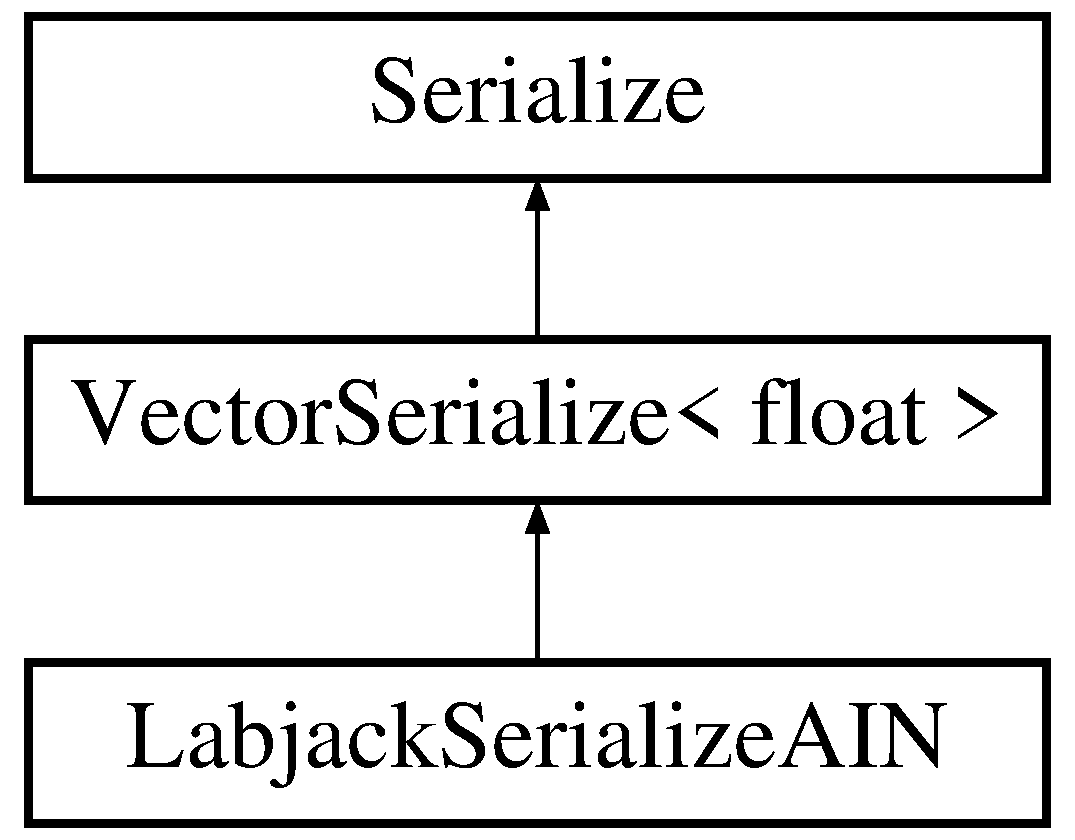
\includegraphics[height=3.000000cm]{classLabjackSerializeAIN}
\end{center}
\end{figure}
\subsection*{Public Member Functions}
\begin{DoxyCompactItemize}
\item 
\hyperlink{classLabjackSerializeAIN_a5e6b1444fe9a1dfe27bad2ed84ee7778}{Labjack\-Serialize\-A\-I\-N} (int nsensors)
\item 
\hyperlink{classLabjackSerializeAIN_a89569122c21dc473fcb0cebda38a0172}{$\sim$\-Labjack\-Serialize\-A\-I\-N} ()
\item 
virtual bool \hyperlink{classLabjackSerializeAIN_a12e5f38cd48f38578f46e8cc90576a93}{store} ()
\item 
bool \hyperlink{classLabjackSerializeAIN_a93f06711fe647e87fa026361640badcb}{store} (float $\ast$data)
\item 
virtual string \hyperlink{classLabjackSerializeAIN_a8ff8a30e23acb11137baab14e47b1d4a}{store\-Name} (int indx)
\item 
virtual double $\ast$ \hyperlink{classLabjackSerializeAIN_a5b64792931481c509eb0c2bb86dbc99a}{mmap\-Read} (double $\ast$d)
\end{DoxyCompactItemize}
\subsection*{Public Attributes}
\begin{DoxyCompactItemize}
\item 
int \hyperlink{classLabjackSerializeAIN_a85aea591bf54bc75577a2a090ce89369}{m\-\_\-nsensors}
\end{DoxyCompactItemize}


\subsection{Constructor \& Destructor Documentation}
\hypertarget{classLabjackSerializeAIN_a5e6b1444fe9a1dfe27bad2ed84ee7778}{\index{Labjack\-Serialize\-A\-I\-N@{Labjack\-Serialize\-A\-I\-N}!Labjack\-Serialize\-A\-I\-N@{Labjack\-Serialize\-A\-I\-N}}
\index{Labjack\-Serialize\-A\-I\-N@{Labjack\-Serialize\-A\-I\-N}!LabjackSerializeAIN@{Labjack\-Serialize\-A\-I\-N}}
\subsubsection[{Labjack\-Serialize\-A\-I\-N}]{\setlength{\rightskip}{0pt plus 5cm}Labjack\-Serialize\-A\-I\-N\-::\-Labjack\-Serialize\-A\-I\-N (
\begin{DoxyParamCaption}
\item[{int}]{nsensors}
\end{DoxyParamCaption}
)}}\label{classLabjackSerializeAIN_a5e6b1444fe9a1dfe27bad2ed84ee7778}
\hypertarget{classLabjackSerializeAIN_a89569122c21dc473fcb0cebda38a0172}{\index{Labjack\-Serialize\-A\-I\-N@{Labjack\-Serialize\-A\-I\-N}!$\sim$\-Labjack\-Serialize\-A\-I\-N@{$\sim$\-Labjack\-Serialize\-A\-I\-N}}
\index{$\sim$\-Labjack\-Serialize\-A\-I\-N@{$\sim$\-Labjack\-Serialize\-A\-I\-N}!LabjackSerializeAIN@{Labjack\-Serialize\-A\-I\-N}}
\subsubsection[{$\sim$\-Labjack\-Serialize\-A\-I\-N}]{\setlength{\rightskip}{0pt plus 5cm}Labjack\-Serialize\-A\-I\-N\-::$\sim$\-Labjack\-Serialize\-A\-I\-N (
\begin{DoxyParamCaption}
{}
\end{DoxyParamCaption}
)}}\label{classLabjackSerializeAIN_a89569122c21dc473fcb0cebda38a0172}


\subsection{Member Function Documentation}
\hypertarget{classLabjackSerializeAIN_a5b64792931481c509eb0c2bb86dbc99a}{\index{Labjack\-Serialize\-A\-I\-N@{Labjack\-Serialize\-A\-I\-N}!mmap\-Read@{mmap\-Read}}
\index{mmap\-Read@{mmap\-Read}!LabjackSerializeAIN@{Labjack\-Serialize\-A\-I\-N}}
\subsubsection[{mmap\-Read}]{\setlength{\rightskip}{0pt plus 5cm}double $\ast$ Labjack\-Serialize\-A\-I\-N\-::mmap\-Read (
\begin{DoxyParamCaption}
\item[{double $\ast$}]{d}
\end{DoxyParamCaption}
)\hspace{0.3cm}{\ttfamily [virtual]}}}\label{classLabjackSerializeAIN_a5b64792931481c509eb0c2bb86dbc99a}


Reimplemented from \hyperlink{classVectorSerialize_a087c30b15095d1b230705e42123eb3db}{Vector\-Serialize$<$ float $>$}.

\hypertarget{classLabjackSerializeAIN_a12e5f38cd48f38578f46e8cc90576a93}{\index{Labjack\-Serialize\-A\-I\-N@{Labjack\-Serialize\-A\-I\-N}!store@{store}}
\index{store@{store}!LabjackSerializeAIN@{Labjack\-Serialize\-A\-I\-N}}
\subsubsection[{store}]{\setlength{\rightskip}{0pt plus 5cm}bool Labjack\-Serialize\-A\-I\-N\-::store (
\begin{DoxyParamCaption}
{}
\end{DoxyParamCaption}
)\hspace{0.3cm}{\ttfamily [virtual]}}}\label{classLabjackSerializeAIN_a12e5f38cd48f38578f46e8cc90576a93}


Reimplemented from \hyperlink{classVectorSerialize_afd6b6dc8768969dae5f27f46eeab83e6}{Vector\-Serialize$<$ float $>$}.

\hypertarget{classLabjackSerializeAIN_a93f06711fe647e87fa026361640badcb}{\index{Labjack\-Serialize\-A\-I\-N@{Labjack\-Serialize\-A\-I\-N}!store@{store}}
\index{store@{store}!LabjackSerializeAIN@{Labjack\-Serialize\-A\-I\-N}}
\subsubsection[{store}]{\setlength{\rightskip}{0pt plus 5cm}bool Labjack\-Serialize\-A\-I\-N\-::store (
\begin{DoxyParamCaption}
\item[{float $\ast$}]{data}
\end{DoxyParamCaption}
)}}\label{classLabjackSerializeAIN_a93f06711fe647e87fa026361640badcb}
\hypertarget{classLabjackSerializeAIN_a8ff8a30e23acb11137baab14e47b1d4a}{\index{Labjack\-Serialize\-A\-I\-N@{Labjack\-Serialize\-A\-I\-N}!store\-Name@{store\-Name}}
\index{store\-Name@{store\-Name}!LabjackSerializeAIN@{Labjack\-Serialize\-A\-I\-N}}
\subsubsection[{store\-Name}]{\setlength{\rightskip}{0pt plus 5cm}string Labjack\-Serialize\-A\-I\-N\-::store\-Name (
\begin{DoxyParamCaption}
\item[{int}]{indx}
\end{DoxyParamCaption}
)\hspace{0.3cm}{\ttfamily [virtual]}}}\label{classLabjackSerializeAIN_a8ff8a30e23acb11137baab14e47b1d4a}


Reimplemented from \hyperlink{classVectorSerialize_a929f94f68d0a99c61308520a679ae1a2}{Vector\-Serialize$<$ float $>$}.



\subsection{Member Data Documentation}
\hypertarget{classLabjackSerializeAIN_a85aea591bf54bc75577a2a090ce89369}{\index{Labjack\-Serialize\-A\-I\-N@{Labjack\-Serialize\-A\-I\-N}!m\-\_\-nsensors@{m\-\_\-nsensors}}
\index{m\-\_\-nsensors@{m\-\_\-nsensors}!LabjackSerializeAIN@{Labjack\-Serialize\-A\-I\-N}}
\subsubsection[{m\-\_\-nsensors}]{\setlength{\rightskip}{0pt plus 5cm}int Labjack\-Serialize\-A\-I\-N\-::m\-\_\-nsensors}}\label{classLabjackSerializeAIN_a85aea591bf54bc75577a2a090ce89369}


The documentation for this class was generated from the following files\-:\begin{DoxyCompactItemize}
\item 
/home/ruijan/sw/bmi5/bmi5/include/\-Serialize/\hyperlink{labjackSerializeAIN_8h}{labjack\-Serialize\-A\-I\-N.\-h}\item 
/home/ruijan/sw/bmi5/bmi5/src/\-Serialize/\hyperlink{labjackSerializeAIN_8cpp}{labjack\-Serialize\-A\-I\-N.\-cpp}\end{DoxyCompactItemize}

\hypertarget{classLabjackSerializeDOUT}{\section{Labjack\-Serialize\-D\-O\-U\-T Class Reference}
\label{classLabjackSerializeDOUT}\index{Labjack\-Serialize\-D\-O\-U\-T@{Labjack\-Serialize\-D\-O\-U\-T}}
}


{\ttfamily \#include $<$labjack\-Serialize\-D\-O\-U\-T.\-h$>$}

Inheritance diagram for Labjack\-Serialize\-D\-O\-U\-T\-:\begin{figure}[H]
\begin{center}
\leavevmode
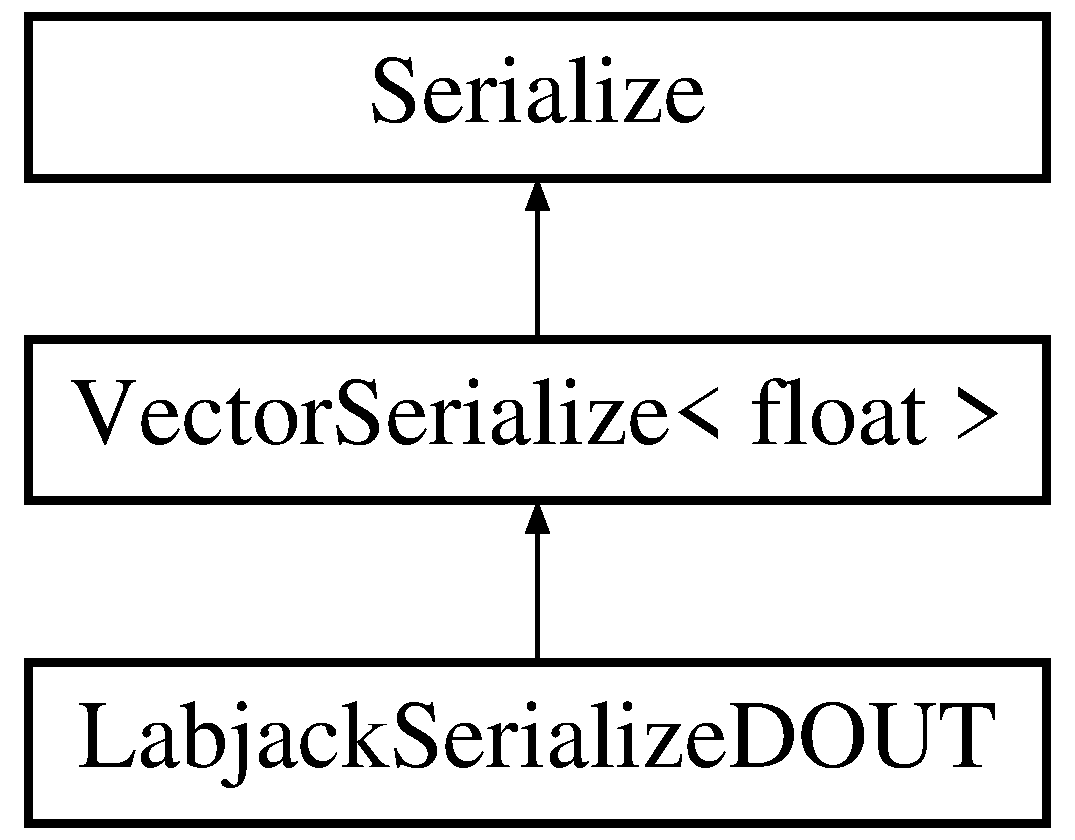
\includegraphics[height=3.000000cm]{classLabjackSerializeDOUT}
\end{center}
\end{figure}
\subsection*{Public Member Functions}
\begin{DoxyCompactItemize}
\item 
\hyperlink{classLabjackSerializeDOUT_a2248473be559c7a1136d52305beb367a}{Labjack\-Serialize\-D\-O\-U\-T} (int nchannels)
\item 
\hyperlink{classLabjackSerializeDOUT_ac6519ba80cc0a5123f59f9d3350911bb}{$\sim$\-Labjack\-Serialize\-D\-O\-U\-T} ()
\item 
virtual bool \hyperlink{classLabjackSerializeDOUT_a2f896d9076b742cbc6fb58faf7cc7b91}{store} ()
\item 
virtual string \hyperlink{classLabjackSerializeDOUT_a814b35d1f45892f684767461d1e8c8a7}{store\-Name} (int indx)
\item 
virtual double $\ast$ \hyperlink{classLabjackSerializeDOUT_a8936d25baa4652bb431b02ccb60489be}{mmap\-Read} (double $\ast$d)
\end{DoxyCompactItemize}
\subsection*{Public Attributes}
\begin{DoxyCompactItemize}
\item 
int \hyperlink{classLabjackSerializeDOUT_afa4c15de49c4dffca161af7f0c8f1099}{m\-\_\-nchannels}
\end{DoxyCompactItemize}


\subsection{Constructor \& Destructor Documentation}
\hypertarget{classLabjackSerializeDOUT_a2248473be559c7a1136d52305beb367a}{\index{Labjack\-Serialize\-D\-O\-U\-T@{Labjack\-Serialize\-D\-O\-U\-T}!Labjack\-Serialize\-D\-O\-U\-T@{Labjack\-Serialize\-D\-O\-U\-T}}
\index{Labjack\-Serialize\-D\-O\-U\-T@{Labjack\-Serialize\-D\-O\-U\-T}!LabjackSerializeDOUT@{Labjack\-Serialize\-D\-O\-U\-T}}
\subsubsection[{Labjack\-Serialize\-D\-O\-U\-T}]{\setlength{\rightskip}{0pt plus 5cm}Labjack\-Serialize\-D\-O\-U\-T\-::\-Labjack\-Serialize\-D\-O\-U\-T (
\begin{DoxyParamCaption}
\item[{int}]{nchannels}
\end{DoxyParamCaption}
)}}\label{classLabjackSerializeDOUT_a2248473be559c7a1136d52305beb367a}
\hypertarget{classLabjackSerializeDOUT_ac6519ba80cc0a5123f59f9d3350911bb}{\index{Labjack\-Serialize\-D\-O\-U\-T@{Labjack\-Serialize\-D\-O\-U\-T}!$\sim$\-Labjack\-Serialize\-D\-O\-U\-T@{$\sim$\-Labjack\-Serialize\-D\-O\-U\-T}}
\index{$\sim$\-Labjack\-Serialize\-D\-O\-U\-T@{$\sim$\-Labjack\-Serialize\-D\-O\-U\-T}!LabjackSerializeDOUT@{Labjack\-Serialize\-D\-O\-U\-T}}
\subsubsection[{$\sim$\-Labjack\-Serialize\-D\-O\-U\-T}]{\setlength{\rightskip}{0pt plus 5cm}Labjack\-Serialize\-D\-O\-U\-T\-::$\sim$\-Labjack\-Serialize\-D\-O\-U\-T (
\begin{DoxyParamCaption}
{}
\end{DoxyParamCaption}
)}}\label{classLabjackSerializeDOUT_ac6519ba80cc0a5123f59f9d3350911bb}


\subsection{Member Function Documentation}
\hypertarget{classLabjackSerializeDOUT_a8936d25baa4652bb431b02ccb60489be}{\index{Labjack\-Serialize\-D\-O\-U\-T@{Labjack\-Serialize\-D\-O\-U\-T}!mmap\-Read@{mmap\-Read}}
\index{mmap\-Read@{mmap\-Read}!LabjackSerializeDOUT@{Labjack\-Serialize\-D\-O\-U\-T}}
\subsubsection[{mmap\-Read}]{\setlength{\rightskip}{0pt plus 5cm}double $\ast$ Labjack\-Serialize\-D\-O\-U\-T\-::mmap\-Read (
\begin{DoxyParamCaption}
\item[{double $\ast$}]{d}
\end{DoxyParamCaption}
)\hspace{0.3cm}{\ttfamily [virtual]}}}\label{classLabjackSerializeDOUT_a8936d25baa4652bb431b02ccb60489be}


Reimplemented from \hyperlink{classVectorSerialize_a087c30b15095d1b230705e42123eb3db}{Vector\-Serialize$<$ float $>$}.

\hypertarget{classLabjackSerializeDOUT_a2f896d9076b742cbc6fb58faf7cc7b91}{\index{Labjack\-Serialize\-D\-O\-U\-T@{Labjack\-Serialize\-D\-O\-U\-T}!store@{store}}
\index{store@{store}!LabjackSerializeDOUT@{Labjack\-Serialize\-D\-O\-U\-T}}
\subsubsection[{store}]{\setlength{\rightskip}{0pt plus 5cm}bool Labjack\-Serialize\-D\-O\-U\-T\-::store (
\begin{DoxyParamCaption}
{}
\end{DoxyParamCaption}
)\hspace{0.3cm}{\ttfamily [virtual]}}}\label{classLabjackSerializeDOUT_a2f896d9076b742cbc6fb58faf7cc7b91}


Reimplemented from \hyperlink{classVectorSerialize_afd6b6dc8768969dae5f27f46eeab83e6}{Vector\-Serialize$<$ float $>$}.

\hypertarget{classLabjackSerializeDOUT_a814b35d1f45892f684767461d1e8c8a7}{\index{Labjack\-Serialize\-D\-O\-U\-T@{Labjack\-Serialize\-D\-O\-U\-T}!store\-Name@{store\-Name}}
\index{store\-Name@{store\-Name}!LabjackSerializeDOUT@{Labjack\-Serialize\-D\-O\-U\-T}}
\subsubsection[{store\-Name}]{\setlength{\rightskip}{0pt plus 5cm}string Labjack\-Serialize\-D\-O\-U\-T\-::store\-Name (
\begin{DoxyParamCaption}
\item[{int}]{indx}
\end{DoxyParamCaption}
)\hspace{0.3cm}{\ttfamily [virtual]}}}\label{classLabjackSerializeDOUT_a814b35d1f45892f684767461d1e8c8a7}


Reimplemented from \hyperlink{classVectorSerialize_a929f94f68d0a99c61308520a679ae1a2}{Vector\-Serialize$<$ float $>$}.



\subsection{Member Data Documentation}
\hypertarget{classLabjackSerializeDOUT_afa4c15de49c4dffca161af7f0c8f1099}{\index{Labjack\-Serialize\-D\-O\-U\-T@{Labjack\-Serialize\-D\-O\-U\-T}!m\-\_\-nchannels@{m\-\_\-nchannels}}
\index{m\-\_\-nchannels@{m\-\_\-nchannels}!LabjackSerializeDOUT@{Labjack\-Serialize\-D\-O\-U\-T}}
\subsubsection[{m\-\_\-nchannels}]{\setlength{\rightskip}{0pt plus 5cm}int Labjack\-Serialize\-D\-O\-U\-T\-::m\-\_\-nchannels}}\label{classLabjackSerializeDOUT_afa4c15de49c4dffca161af7f0c8f1099}


The documentation for this class was generated from the following files\-:\begin{DoxyCompactItemize}
\item 
/home/ruijan/sw/bmi5/bmi5/include/\-Serialize/\hyperlink{labjackSerializeDOUT_8h}{labjack\-Serialize\-D\-O\-U\-T.\-h}\item 
/home/ruijan/sw/bmi5/bmi5/src/\-Serialize/\hyperlink{labjackSerializeDOUT_8cpp}{labjack\-Serialize\-D\-O\-U\-T.\-cpp}\end{DoxyCompactItemize}

\hypertarget{classLine}{\section{Line Class Reference}
\label{classLine}\index{Line@{Line}}
}


{\ttfamily \#include $<$line.\-h$>$}

Inheritance diagram for Line\-:\begin{figure}[H]
\begin{center}
\leavevmode
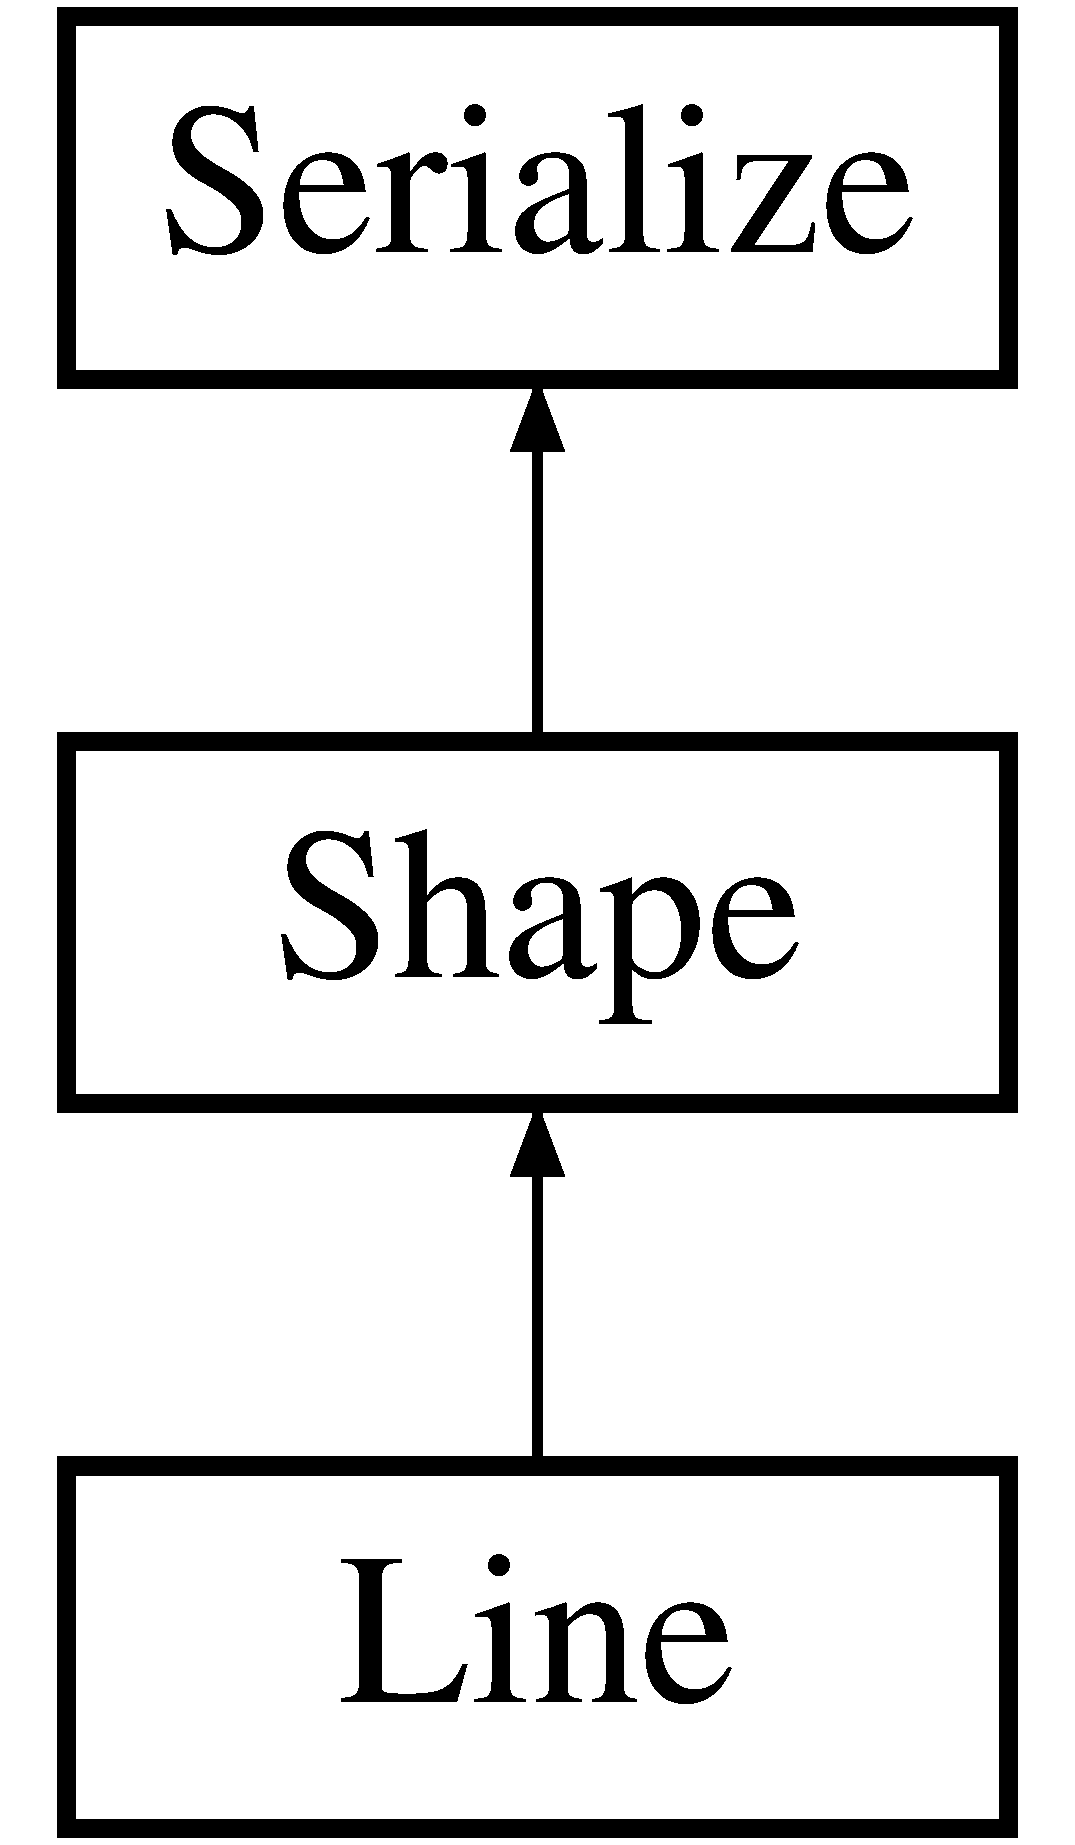
\includegraphics[height=3.000000cm]{classLine}
\end{center}
\end{figure}
\subsection*{Public Member Functions}
\begin{DoxyCompactItemize}
\item 
\hyperlink{classLine_af13fbd7711414690b1ba1527636009ab}{Line} (float length)
\item 
virtual \hyperlink{classLine_aabe85f48d22d92b62257091f48174fac}{$\sim$\-Line} ()
\item 
virtual void \hyperlink{classLine_a3f357683e8a9700cfc4d6f65f7f9493f}{fill} (float $\ast$v)
\end{DoxyCompactItemize}
\subsection*{Private Attributes}
\begin{DoxyCompactItemize}
\item 
float \hyperlink{classLine_ab7c1828bc8bc4e3647dfdd963c17d555}{m\-\_\-l}
\end{DoxyCompactItemize}
\subsection*{Additional Inherited Members}


\subsection{Constructor \& Destructor Documentation}
\hypertarget{classLine_af13fbd7711414690b1ba1527636009ab}{\index{Line@{Line}!Line@{Line}}
\index{Line@{Line}!Line@{Line}}
\subsubsection[{Line}]{\setlength{\rightskip}{0pt plus 5cm}Line\-::\-Line (
\begin{DoxyParamCaption}
\item[{float}]{length}
\end{DoxyParamCaption}
)}}\label{classLine_af13fbd7711414690b1ba1527636009ab}
\hypertarget{classLine_aabe85f48d22d92b62257091f48174fac}{\index{Line@{Line}!$\sim$\-Line@{$\sim$\-Line}}
\index{$\sim$\-Line@{$\sim$\-Line}!Line@{Line}}
\subsubsection[{$\sim$\-Line}]{\setlength{\rightskip}{0pt plus 5cm}Line\-::$\sim$\-Line (
\begin{DoxyParamCaption}
{}
\end{DoxyParamCaption}
)\hspace{0.3cm}{\ttfamily [virtual]}}}\label{classLine_aabe85f48d22d92b62257091f48174fac}


\subsection{Member Function Documentation}
\hypertarget{classLine_a3f357683e8a9700cfc4d6f65f7f9493f}{\index{Line@{Line}!fill@{fill}}
\index{fill@{fill}!Line@{Line}}
\subsubsection[{fill}]{\setlength{\rightskip}{0pt plus 5cm}void Line\-::fill (
\begin{DoxyParamCaption}
\item[{float $\ast$}]{v}
\end{DoxyParamCaption}
)\hspace{0.3cm}{\ttfamily [virtual]}}}\label{classLine_a3f357683e8a9700cfc4d6f65f7f9493f}


Reimplemented from \hyperlink{classShape_a33be64d8e24518084b1c8f974f808387}{Shape}.



\subsection{Member Data Documentation}
\hypertarget{classLine_ab7c1828bc8bc4e3647dfdd963c17d555}{\index{Line@{Line}!m\-\_\-l@{m\-\_\-l}}
\index{m\-\_\-l@{m\-\_\-l}!Line@{Line}}
\subsubsection[{m\-\_\-l}]{\setlength{\rightskip}{0pt plus 5cm}float Line\-::m\-\_\-l\hspace{0.3cm}{\ttfamily [private]}}}\label{classLine_ab7c1828bc8bc4e3647dfdd963c17d555}


The documentation for this class was generated from the following files\-:\begin{DoxyCompactItemize}
\item 
/home/ruijan/sw/bmi5/bmi5/include/\-Shape/\hyperlink{line_8h}{line.\-h}\item 
/home/ruijan/sw/bmi5/bmi5/src/\-Shape/\hyperlink{line_8cpp}{line.\-cpp}\end{DoxyCompactItemize}

\hypertarget{classMatrix44Serialize}{\section{Matrix44\-Serialize Class Reference}
\label{classMatrix44Serialize}\index{Matrix44\-Serialize@{Matrix44\-Serialize}}
}


{\ttfamily \#include $<$matrix44\-Serialize.\-h$>$}

Inheritance diagram for Matrix44\-Serialize\-:\begin{figure}[H]
\begin{center}
\leavevmode
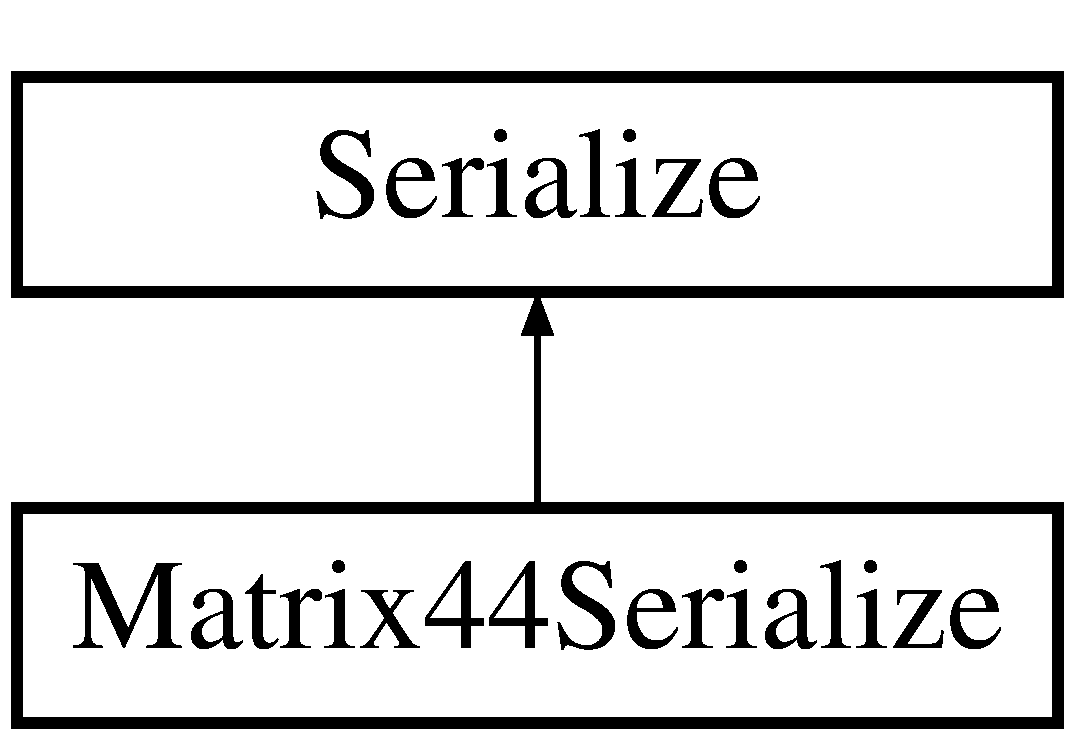
\includegraphics[height=2.000000cm]{classMatrix44Serialize}
\end{center}
\end{figure}
\subsection*{Public Member Functions}
\begin{DoxyCompactItemize}
\item 
\hyperlink{classMatrix44Serialize_a0bcff20c12377cecee29099007ab5fc7}{Matrix44\-Serialize} (string name)
\item 
\hyperlink{classMatrix44Serialize_a9d0a79d7f215cbcc763e777cf0379fb8}{$\sim$\-Matrix44\-Serialize} ()
\item 
virtual void \hyperlink{classMatrix44Serialize_aaea63fa835d82cc7d039323e678ec58a}{clear} ()
\item 
virtual bool \hyperlink{classMatrix44Serialize_a96da5f524e0e2522085f82b20f6e3de0}{store} ()
\item 
virtual int \hyperlink{classMatrix44Serialize_ab1531b0cb71530688376e3b5f9e05076}{nstored} ()
\item 
virtual string \hyperlink{classMatrix44Serialize_a1262b03de3cf08dab616bdb44b354d3d}{store\-Name} (int)
\item 
virtual int \hyperlink{classMatrix44Serialize_a543c479bc5f47c7045988f14dc398cfa}{get\-Store\-Class} (int)
\item 
virtual void \hyperlink{classMatrix44Serialize_ad2a049be2ae27daad403c7e1d7ca4de0}{get\-Store\-Dims} (int, size\-\_\-t $\ast$dims)
\item 
virtual void $\ast$ \hyperlink{classMatrix44Serialize_a4690b73080db8812c3ca0970f05c699d}{get\-Store} (int, int k)
\item 
virtual int \hyperlink{classMatrix44Serialize_aa87157b168588ba1e29d6dee6529e906}{num\-Stores} ()
\item 
virtual double $\ast$ \hyperlink{classMatrix44Serialize_a9882ee2bdc032d63cc2daf6eb25a7464}{mmap\-Read} (double $\ast$d)
\item 
float $\ast$ \hyperlink{classMatrix44Serialize_aec8417e383b9da42858da90c26144f8b}{data} ()
\end{DoxyCompactItemize}
\subsection*{Public Attributes}
\begin{DoxyCompactItemize}
\item 
array$<$ double, 16 $>$ \hyperlink{classMatrix44Serialize_a887ffc59342dfab5667c068ece0bc9e4}{m\-\_\-cmp}
\item 
array$<$ float, 16 $>$ \hyperlink{classMatrix44Serialize_a71fe9d20c4d708809ffdea76e6e4e14b}{m\-\_\-x}
\item 
vector$<$ array$<$ float, 16 $>$ $>$ \hyperlink{classMatrix44Serialize_abc347705129a270f25ec5d07cc5f0846}{v\-\_\-x}
\end{DoxyCompactItemize}


\subsection{Constructor \& Destructor Documentation}
\hypertarget{classMatrix44Serialize_a0bcff20c12377cecee29099007ab5fc7}{\index{Matrix44\-Serialize@{Matrix44\-Serialize}!Matrix44\-Serialize@{Matrix44\-Serialize}}
\index{Matrix44\-Serialize@{Matrix44\-Serialize}!Matrix44Serialize@{Matrix44\-Serialize}}
\subsubsection[{Matrix44\-Serialize}]{\setlength{\rightskip}{0pt plus 5cm}Matrix44\-Serialize\-::\-Matrix44\-Serialize (
\begin{DoxyParamCaption}
\item[{string}]{name}
\end{DoxyParamCaption}
)}}\label{classMatrix44Serialize_a0bcff20c12377cecee29099007ab5fc7}
\hypertarget{classMatrix44Serialize_a9d0a79d7f215cbcc763e777cf0379fb8}{\index{Matrix44\-Serialize@{Matrix44\-Serialize}!$\sim$\-Matrix44\-Serialize@{$\sim$\-Matrix44\-Serialize}}
\index{$\sim$\-Matrix44\-Serialize@{$\sim$\-Matrix44\-Serialize}!Matrix44Serialize@{Matrix44\-Serialize}}
\subsubsection[{$\sim$\-Matrix44\-Serialize}]{\setlength{\rightskip}{0pt plus 5cm}Matrix44\-Serialize\-::$\sim$\-Matrix44\-Serialize (
\begin{DoxyParamCaption}
{}
\end{DoxyParamCaption}
)}}\label{classMatrix44Serialize_a9d0a79d7f215cbcc763e777cf0379fb8}


\subsection{Member Function Documentation}
\hypertarget{classMatrix44Serialize_aaea63fa835d82cc7d039323e678ec58a}{\index{Matrix44\-Serialize@{Matrix44\-Serialize}!clear@{clear}}
\index{clear@{clear}!Matrix44Serialize@{Matrix44\-Serialize}}
\subsubsection[{clear}]{\setlength{\rightskip}{0pt plus 5cm}void Matrix44\-Serialize\-::clear (
\begin{DoxyParamCaption}
{}
\end{DoxyParamCaption}
)\hspace{0.3cm}{\ttfamily [virtual]}}}\label{classMatrix44Serialize_aaea63fa835d82cc7d039323e678ec58a}


Reimplemented from \hyperlink{classSerialize_a11cbf006415c08d1891ab42e39a2aa1a}{Serialize}.

\hypertarget{classMatrix44Serialize_aec8417e383b9da42858da90c26144f8b}{\index{Matrix44\-Serialize@{Matrix44\-Serialize}!data@{data}}
\index{data@{data}!Matrix44Serialize@{Matrix44\-Serialize}}
\subsubsection[{data}]{\setlength{\rightskip}{0pt plus 5cm}float $\ast$ Matrix44\-Serialize\-::data (
\begin{DoxyParamCaption}
{}
\end{DoxyParamCaption}
)}}\label{classMatrix44Serialize_aec8417e383b9da42858da90c26144f8b}
\hypertarget{classMatrix44Serialize_a4690b73080db8812c3ca0970f05c699d}{\index{Matrix44\-Serialize@{Matrix44\-Serialize}!get\-Store@{get\-Store}}
\index{get\-Store@{get\-Store}!Matrix44Serialize@{Matrix44\-Serialize}}
\subsubsection[{get\-Store}]{\setlength{\rightskip}{0pt plus 5cm}void $\ast$ Matrix44\-Serialize\-::get\-Store (
\begin{DoxyParamCaption}
\item[{int}]{, }
\item[{int}]{k}
\end{DoxyParamCaption}
)\hspace{0.3cm}{\ttfamily [virtual]}}}\label{classMatrix44Serialize_a4690b73080db8812c3ca0970f05c699d}


Reimplemented from \hyperlink{classSerialize_a6e589d263cfdc0eb72e41687c58831f2}{Serialize}.

\hypertarget{classMatrix44Serialize_a543c479bc5f47c7045988f14dc398cfa}{\index{Matrix44\-Serialize@{Matrix44\-Serialize}!get\-Store\-Class@{get\-Store\-Class}}
\index{get\-Store\-Class@{get\-Store\-Class}!Matrix44Serialize@{Matrix44\-Serialize}}
\subsubsection[{get\-Store\-Class}]{\setlength{\rightskip}{0pt plus 5cm}int Matrix44\-Serialize\-::get\-Store\-Class (
\begin{DoxyParamCaption}
\item[{int}]{}
\end{DoxyParamCaption}
)\hspace{0.3cm}{\ttfamily [virtual]}}}\label{classMatrix44Serialize_a543c479bc5f47c7045988f14dc398cfa}


Reimplemented from \hyperlink{classSerialize_a69954cc86d03b75b6b27511aec4aba43}{Serialize}.

\hypertarget{classMatrix44Serialize_ad2a049be2ae27daad403c7e1d7ca4de0}{\index{Matrix44\-Serialize@{Matrix44\-Serialize}!get\-Store\-Dims@{get\-Store\-Dims}}
\index{get\-Store\-Dims@{get\-Store\-Dims}!Matrix44Serialize@{Matrix44\-Serialize}}
\subsubsection[{get\-Store\-Dims}]{\setlength{\rightskip}{0pt plus 5cm}void Matrix44\-Serialize\-::get\-Store\-Dims (
\begin{DoxyParamCaption}
\item[{int}]{, }
\item[{size\-\_\-t $\ast$}]{dims}
\end{DoxyParamCaption}
)\hspace{0.3cm}{\ttfamily [virtual]}}}\label{classMatrix44Serialize_ad2a049be2ae27daad403c7e1d7ca4de0}


Reimplemented from \hyperlink{classSerialize_a52034c5c17bc5e7e6c728b4e6c620c05}{Serialize}.

\hypertarget{classMatrix44Serialize_a9882ee2bdc032d63cc2daf6eb25a7464}{\index{Matrix44\-Serialize@{Matrix44\-Serialize}!mmap\-Read@{mmap\-Read}}
\index{mmap\-Read@{mmap\-Read}!Matrix44Serialize@{Matrix44\-Serialize}}
\subsubsection[{mmap\-Read}]{\setlength{\rightskip}{0pt plus 5cm}double $\ast$ Matrix44\-Serialize\-::mmap\-Read (
\begin{DoxyParamCaption}
\item[{double $\ast$}]{d}
\end{DoxyParamCaption}
)\hspace{0.3cm}{\ttfamily [virtual]}}}\label{classMatrix44Serialize_a9882ee2bdc032d63cc2daf6eb25a7464}


Reimplemented from \hyperlink{classSerialize_a28b939242880e565a8906b30acd0f84c}{Serialize}.

\hypertarget{classMatrix44Serialize_ab1531b0cb71530688376e3b5f9e05076}{\index{Matrix44\-Serialize@{Matrix44\-Serialize}!nstored@{nstored}}
\index{nstored@{nstored}!Matrix44Serialize@{Matrix44\-Serialize}}
\subsubsection[{nstored}]{\setlength{\rightskip}{0pt plus 5cm}int Matrix44\-Serialize\-::nstored (
\begin{DoxyParamCaption}
{}
\end{DoxyParamCaption}
)\hspace{0.3cm}{\ttfamily [virtual]}}}\label{classMatrix44Serialize_ab1531b0cb71530688376e3b5f9e05076}


Reimplemented from \hyperlink{classSerialize_a590b7308112b07581c03ba826ace50b4}{Serialize}.

\hypertarget{classMatrix44Serialize_aa87157b168588ba1e29d6dee6529e906}{\index{Matrix44\-Serialize@{Matrix44\-Serialize}!num\-Stores@{num\-Stores}}
\index{num\-Stores@{num\-Stores}!Matrix44Serialize@{Matrix44\-Serialize}}
\subsubsection[{num\-Stores}]{\setlength{\rightskip}{0pt plus 5cm}int Matrix44\-Serialize\-::num\-Stores (
\begin{DoxyParamCaption}
{}
\end{DoxyParamCaption}
)\hspace{0.3cm}{\ttfamily [virtual]}}}\label{classMatrix44Serialize_aa87157b168588ba1e29d6dee6529e906}


Reimplemented from \hyperlink{classSerialize_a71bf2a906fd71477308a942d01490ab3}{Serialize}.

\hypertarget{classMatrix44Serialize_a96da5f524e0e2522085f82b20f6e3de0}{\index{Matrix44\-Serialize@{Matrix44\-Serialize}!store@{store}}
\index{store@{store}!Matrix44Serialize@{Matrix44\-Serialize}}
\subsubsection[{store}]{\setlength{\rightskip}{0pt plus 5cm}bool Matrix44\-Serialize\-::store (
\begin{DoxyParamCaption}
{}
\end{DoxyParamCaption}
)\hspace{0.3cm}{\ttfamily [virtual]}}}\label{classMatrix44Serialize_a96da5f524e0e2522085f82b20f6e3de0}


Reimplemented from \hyperlink{classSerialize_a3cda20e84a530870a6115eaaf589f168}{Serialize}.

\hypertarget{classMatrix44Serialize_a1262b03de3cf08dab616bdb44b354d3d}{\index{Matrix44\-Serialize@{Matrix44\-Serialize}!store\-Name@{store\-Name}}
\index{store\-Name@{store\-Name}!Matrix44Serialize@{Matrix44\-Serialize}}
\subsubsection[{store\-Name}]{\setlength{\rightskip}{0pt plus 5cm}string Matrix44\-Serialize\-::store\-Name (
\begin{DoxyParamCaption}
\item[{int}]{}
\end{DoxyParamCaption}
)\hspace{0.3cm}{\ttfamily [virtual]}}}\label{classMatrix44Serialize_a1262b03de3cf08dab616bdb44b354d3d}


Reimplemented from \hyperlink{classSerialize_ac94a76de6c9376e33b4c195d50ff0568}{Serialize}.



\subsection{Member Data Documentation}
\hypertarget{classMatrix44Serialize_a887ffc59342dfab5667c068ece0bc9e4}{\index{Matrix44\-Serialize@{Matrix44\-Serialize}!m\-\_\-cmp@{m\-\_\-cmp}}
\index{m\-\_\-cmp@{m\-\_\-cmp}!Matrix44Serialize@{Matrix44\-Serialize}}
\subsubsection[{m\-\_\-cmp}]{\setlength{\rightskip}{0pt plus 5cm}array$<$double,16$>$ Matrix44\-Serialize\-::m\-\_\-cmp}}\label{classMatrix44Serialize_a887ffc59342dfab5667c068ece0bc9e4}
\hypertarget{classMatrix44Serialize_a71fe9d20c4d708809ffdea76e6e4e14b}{\index{Matrix44\-Serialize@{Matrix44\-Serialize}!m\-\_\-x@{m\-\_\-x}}
\index{m\-\_\-x@{m\-\_\-x}!Matrix44Serialize@{Matrix44\-Serialize}}
\subsubsection[{m\-\_\-x}]{\setlength{\rightskip}{0pt plus 5cm}array$<$float,16$>$ Matrix44\-Serialize\-::m\-\_\-x}}\label{classMatrix44Serialize_a71fe9d20c4d708809ffdea76e6e4e14b}
\hypertarget{classMatrix44Serialize_abc347705129a270f25ec5d07cc5f0846}{\index{Matrix44\-Serialize@{Matrix44\-Serialize}!v\-\_\-x@{v\-\_\-x}}
\index{v\-\_\-x@{v\-\_\-x}!Matrix44Serialize@{Matrix44\-Serialize}}
\subsubsection[{v\-\_\-x}]{\setlength{\rightskip}{0pt plus 5cm}vector$<$array$<$float,16$>$ $>$ Matrix44\-Serialize\-::v\-\_\-x}}\label{classMatrix44Serialize_abc347705129a270f25ec5d07cc5f0846}


The documentation for this class was generated from the following files\-:\begin{DoxyCompactItemize}
\item 
/home/ruijan/sw/bmi5/bmi5/include/\-Serialize/\hyperlink{matrix44Serialize_8h}{matrix44\-Serialize.\-h}\item 
/home/ruijan/sw/bmi5/bmi5/src/\-Serialize/\hyperlink{matrix44Serialize_8cpp}{matrix44\-Serialize.\-cpp}\end{DoxyCompactItemize}

\hypertarget{classMouseSerialize}{\section{Mouse\-Serialize Class Reference}
\label{classMouseSerialize}\index{Mouse\-Serialize@{Mouse\-Serialize}}
}


{\ttfamily \#include $<$mouse\-Serialize.\-h$>$}

Inheritance diagram for Mouse\-Serialize\-:\begin{figure}[H]
\begin{center}
\leavevmode
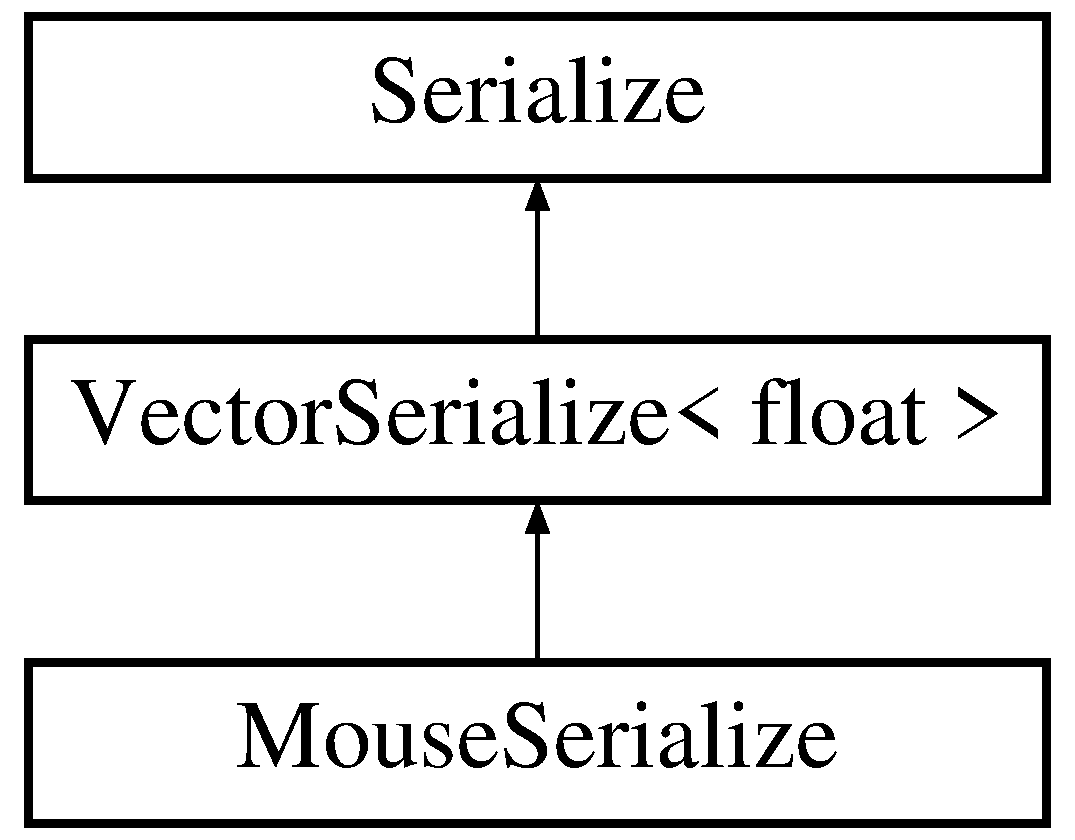
\includegraphics[height=3.000000cm]{classMouseSerialize}
\end{center}
\end{figure}
\subsection*{Public Member Functions}
\begin{DoxyCompactItemize}
\item 
\hyperlink{classMouseSerialize_a93c473c5f51988dd5c6b76d6421ac100}{Mouse\-Serialize} ()
\item 
\hyperlink{classMouseSerialize_a09b6c1b866ff0a0999b860677f88d2c4}{$\sim$\-Mouse\-Serialize} ()
\item 
virtual bool \hyperlink{classMouseSerialize_acfe8874b5ea2c2e4a2f235b7b97780e8}{store} ()
\item 
virtual string \hyperlink{classMouseSerialize_a93bdbce909f27855fd2e8eb6edbf75a0}{store\-Name} (int)
\item 
virtual double $\ast$ \hyperlink{classMouseSerialize_ab919e98d4daf8a068fc68741a4a4dcb7}{mmap\-Read} (double $\ast$d)
\end{DoxyCompactItemize}
\subsection*{Additional Inherited Members}


\subsection{Constructor \& Destructor Documentation}
\hypertarget{classMouseSerialize_a93c473c5f51988dd5c6b76d6421ac100}{\index{Mouse\-Serialize@{Mouse\-Serialize}!Mouse\-Serialize@{Mouse\-Serialize}}
\index{Mouse\-Serialize@{Mouse\-Serialize}!MouseSerialize@{Mouse\-Serialize}}
\subsubsection[{Mouse\-Serialize}]{\setlength{\rightskip}{0pt plus 5cm}Mouse\-Serialize\-::\-Mouse\-Serialize (
\begin{DoxyParamCaption}
{}
\end{DoxyParamCaption}
)}}\label{classMouseSerialize_a93c473c5f51988dd5c6b76d6421ac100}
\hypertarget{classMouseSerialize_a09b6c1b866ff0a0999b860677f88d2c4}{\index{Mouse\-Serialize@{Mouse\-Serialize}!$\sim$\-Mouse\-Serialize@{$\sim$\-Mouse\-Serialize}}
\index{$\sim$\-Mouse\-Serialize@{$\sim$\-Mouse\-Serialize}!MouseSerialize@{Mouse\-Serialize}}
\subsubsection[{$\sim$\-Mouse\-Serialize}]{\setlength{\rightskip}{0pt plus 5cm}Mouse\-Serialize\-::$\sim$\-Mouse\-Serialize (
\begin{DoxyParamCaption}
{}
\end{DoxyParamCaption}
)}}\label{classMouseSerialize_a09b6c1b866ff0a0999b860677f88d2c4}


\subsection{Member Function Documentation}
\hypertarget{classMouseSerialize_ab919e98d4daf8a068fc68741a4a4dcb7}{\index{Mouse\-Serialize@{Mouse\-Serialize}!mmap\-Read@{mmap\-Read}}
\index{mmap\-Read@{mmap\-Read}!MouseSerialize@{Mouse\-Serialize}}
\subsubsection[{mmap\-Read}]{\setlength{\rightskip}{0pt plus 5cm}double $\ast$ Mouse\-Serialize\-::mmap\-Read (
\begin{DoxyParamCaption}
\item[{double $\ast$}]{d}
\end{DoxyParamCaption}
)\hspace{0.3cm}{\ttfamily [virtual]}}}\label{classMouseSerialize_ab919e98d4daf8a068fc68741a4a4dcb7}


Reimplemented from \hyperlink{classVectorSerialize_a087c30b15095d1b230705e42123eb3db}{Vector\-Serialize$<$ float $>$}.

\hypertarget{classMouseSerialize_acfe8874b5ea2c2e4a2f235b7b97780e8}{\index{Mouse\-Serialize@{Mouse\-Serialize}!store@{store}}
\index{store@{store}!MouseSerialize@{Mouse\-Serialize}}
\subsubsection[{store}]{\setlength{\rightskip}{0pt plus 5cm}bool Mouse\-Serialize\-::store (
\begin{DoxyParamCaption}
{}
\end{DoxyParamCaption}
)\hspace{0.3cm}{\ttfamily [virtual]}}}\label{classMouseSerialize_acfe8874b5ea2c2e4a2f235b7b97780e8}


Reimplemented from \hyperlink{classVectorSerialize_afd6b6dc8768969dae5f27f46eeab83e6}{Vector\-Serialize$<$ float $>$}.

\hypertarget{classMouseSerialize_a93bdbce909f27855fd2e8eb6edbf75a0}{\index{Mouse\-Serialize@{Mouse\-Serialize}!store\-Name@{store\-Name}}
\index{store\-Name@{store\-Name}!MouseSerialize@{Mouse\-Serialize}}
\subsubsection[{store\-Name}]{\setlength{\rightskip}{0pt plus 5cm}string Mouse\-Serialize\-::store\-Name (
\begin{DoxyParamCaption}
\item[{int}]{}
\end{DoxyParamCaption}
)\hspace{0.3cm}{\ttfamily [virtual]}}}\label{classMouseSerialize_a93bdbce909f27855fd2e8eb6edbf75a0}


Reimplemented from \hyperlink{classVectorSerialize_a929f94f68d0a99c61308520a679ae1a2}{Vector\-Serialize$<$ float $>$}.



The documentation for this class was generated from the following files\-:\begin{DoxyCompactItemize}
\item 
/home/ruijan/sw/bmi5/bmi5/include/\-Serialize/\hyperlink{mouseSerialize_8h}{mouse\-Serialize.\-h}\item 
/home/ruijan/sw/bmi5/bmi5/src/\-Serialize/\hyperlink{mouseSerialize_8cpp}{mouse\-Serialize.\-cpp}\end{DoxyCompactItemize}

\hypertarget{classOpenSquare}{\section{Open\-Square Class Reference}
\label{classOpenSquare}\index{Open\-Square@{Open\-Square}}
}


{\ttfamily \#include $<$open\-Square.\-h$>$}

Inheritance diagram for Open\-Square\-:\begin{figure}[H]
\begin{center}
\leavevmode
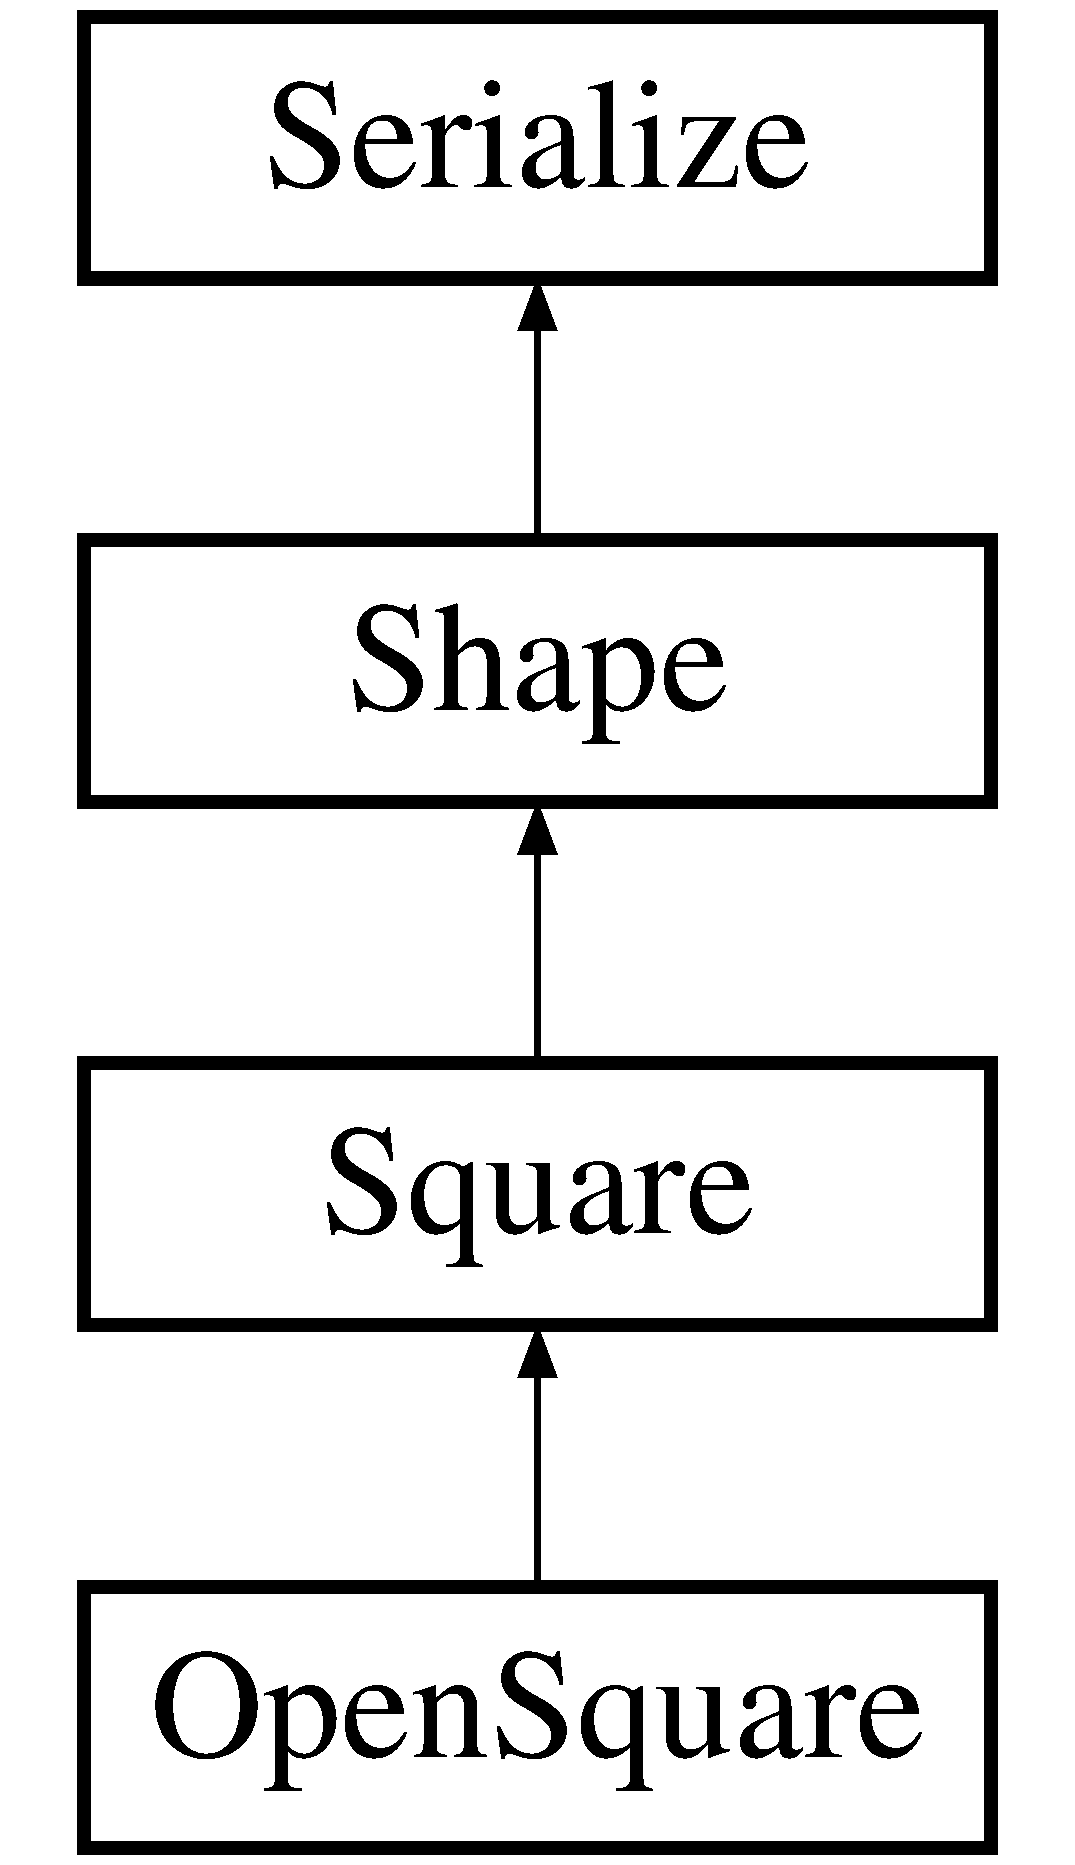
\includegraphics[height=4.000000cm]{classOpenSquare}
\end{center}
\end{figure}
\subsection*{Public Member Functions}
\begin{DoxyCompactItemize}
\item 
\hyperlink{classOpenSquare_a7910e72901054938e84f273856a6a6b9}{Open\-Square} (float inner\-Width, float outer\-Width)
\item 
\hyperlink{classOpenSquare_a9e55d8c84ccc048eac82bcb0c2ec651a}{$\sim$\-Open\-Square} ()
\item 
virtual void \hyperlink{classOpenSquare_aa75c880448b327596b0b5fbde69e561c}{fill} (float $\ast$v)
\end{DoxyCompactItemize}
\subsection*{Private Attributes}
\begin{DoxyCompactItemize}
\item 
float \hyperlink{classOpenSquare_ae85dd099f8da8e1d0b8486067632006a}{m\-\_\-iw}
\end{DoxyCompactItemize}
\subsection*{Additional Inherited Members}


\subsection{Constructor \& Destructor Documentation}
\hypertarget{classOpenSquare_a7910e72901054938e84f273856a6a6b9}{\index{Open\-Square@{Open\-Square}!Open\-Square@{Open\-Square}}
\index{Open\-Square@{Open\-Square}!OpenSquare@{Open\-Square}}
\subsubsection[{Open\-Square}]{\setlength{\rightskip}{0pt plus 5cm}Open\-Square\-::\-Open\-Square (
\begin{DoxyParamCaption}
\item[{float}]{inner\-Width, }
\item[{float}]{outer\-Width}
\end{DoxyParamCaption}
)}}\label{classOpenSquare_a7910e72901054938e84f273856a6a6b9}
\hypertarget{classOpenSquare_a9e55d8c84ccc048eac82bcb0c2ec651a}{\index{Open\-Square@{Open\-Square}!$\sim$\-Open\-Square@{$\sim$\-Open\-Square}}
\index{$\sim$\-Open\-Square@{$\sim$\-Open\-Square}!OpenSquare@{Open\-Square}}
\subsubsection[{$\sim$\-Open\-Square}]{\setlength{\rightskip}{0pt plus 5cm}Open\-Square\-::$\sim$\-Open\-Square (
\begin{DoxyParamCaption}
{}
\end{DoxyParamCaption}
)}}\label{classOpenSquare_a9e55d8c84ccc048eac82bcb0c2ec651a}


\subsection{Member Function Documentation}
\hypertarget{classOpenSquare_aa75c880448b327596b0b5fbde69e561c}{\index{Open\-Square@{Open\-Square}!fill@{fill}}
\index{fill@{fill}!OpenSquare@{Open\-Square}}
\subsubsection[{fill}]{\setlength{\rightskip}{0pt plus 5cm}void Open\-Square\-::fill (
\begin{DoxyParamCaption}
\item[{float $\ast$}]{v}
\end{DoxyParamCaption}
)\hspace{0.3cm}{\ttfamily [virtual]}}}\label{classOpenSquare_aa75c880448b327596b0b5fbde69e561c}


Reimplemented from \hyperlink{classSquare_aedaf26740b0f71c086886d5519cf44a6}{Square}.



\subsection{Member Data Documentation}
\hypertarget{classOpenSquare_ae85dd099f8da8e1d0b8486067632006a}{\index{Open\-Square@{Open\-Square}!m\-\_\-iw@{m\-\_\-iw}}
\index{m\-\_\-iw@{m\-\_\-iw}!OpenSquare@{Open\-Square}}
\subsubsection[{m\-\_\-iw}]{\setlength{\rightskip}{0pt plus 5cm}float Open\-Square\-::m\-\_\-iw\hspace{0.3cm}{\ttfamily [private]}}}\label{classOpenSquare_ae85dd099f8da8e1d0b8486067632006a}


The documentation for this class was generated from the following files\-:\begin{DoxyCompactItemize}
\item 
/home/ruijan/sw/bmi5/bmi5/include/\-Shape/\hyperlink{openSquare_8h}{open\-Square.\-h}\item 
/home/ruijan/sw/bmi5/bmi5/src/\-Shape/\hyperlink{openSquare_8cpp}{open\-Square.\-cpp}\end{DoxyCompactItemize}

\hypertarget{classOptoSerialize}{\section{Opto\-Serialize Class Reference}
\label{classOptoSerialize}\index{Opto\-Serialize@{Opto\-Serialize}}
}


{\ttfamily \#include $<$opto\-Serialize.\-h$>$}

Inheritance diagram for Opto\-Serialize\-:\begin{figure}[H]
\begin{center}
\leavevmode
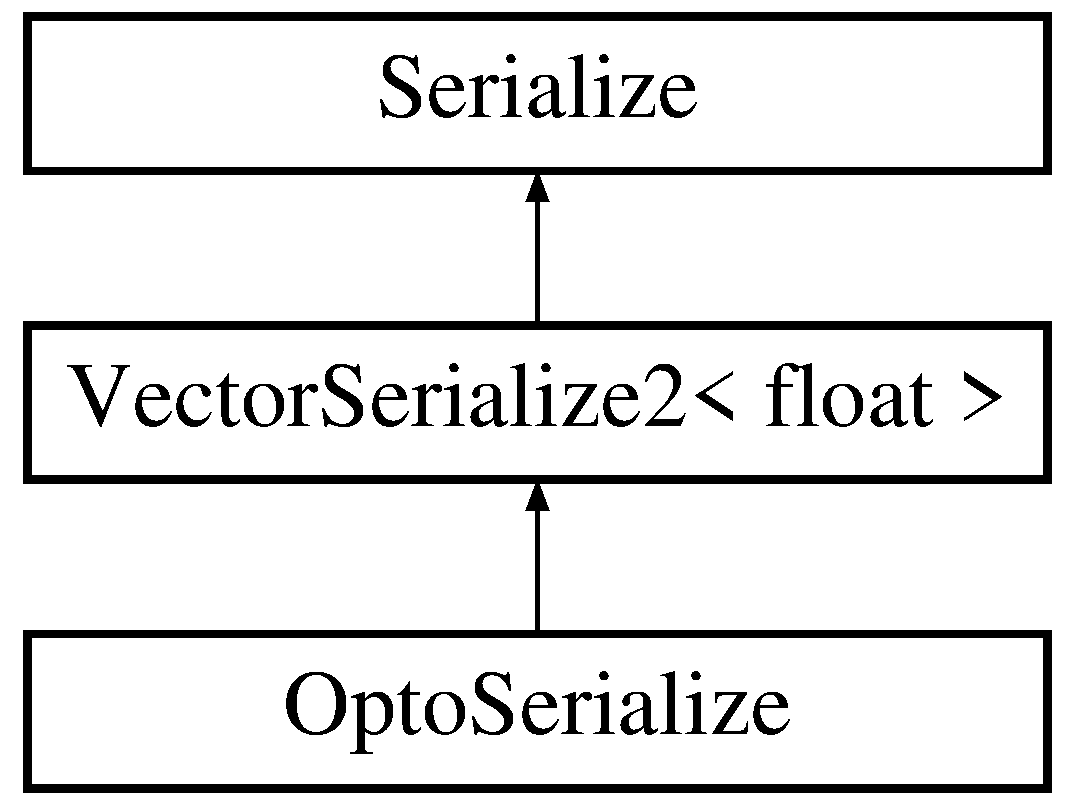
\includegraphics[height=3.000000cm]{classOptoSerialize}
\end{center}
\end{figure}
\subsection*{Public Member Functions}
\begin{DoxyCompactItemize}
\item 
\hyperlink{classOptoSerialize_a4b115e74d86c722fd109b3786bbec847}{Opto\-Serialize} (int nsensors)
\item 
\hyperlink{classOptoSerialize_a28b3097639217d817ea084cc870f34b4}{$\sim$\-Opto\-Serialize} ()
\item 
virtual bool \hyperlink{classOptoSerialize_aef848193a25e0b103e31f8d25035af16}{store} ()
\item 
bool \hyperlink{classOptoSerialize_a57544cacf42315f991a6a1d5bfc69d11}{store} (float $\ast$data)
\item 
void \hyperlink{classOptoSerialize_a3c2758b5a41759414f32a90d514ff5b8}{get\-Loc} (double now, float $\ast$out)
\item 
virtual string \hyperlink{classOptoSerialize_a6a29e96b87575f2906b65be40c38ceb2}{store\-Name} (int indx)
\item 
virtual double $\ast$ \hyperlink{classOptoSerialize_a35e6ee49e354276af9548a759fa3f3d2}{mmap\-Read} (double $\ast$d)
\end{DoxyCompactItemize}
\subsection*{Public Attributes}
\begin{DoxyCompactItemize}
\item 
int \hyperlink{classOptoSerialize_acf6821903586a62e8e3d20ffec81a913}{m\-\_\-nsensors}
\item 
vector$<$ \hyperlink{classPolhemusPredict}{Polhemus\-Predict} $\ast$ $>$ \hyperlink{classOptoSerialize_a161d329d6a8ee02c408e017a7f919a86}{m\-\_\-pp}
\end{DoxyCompactItemize}


\subsection{Constructor \& Destructor Documentation}
\hypertarget{classOptoSerialize_a4b115e74d86c722fd109b3786bbec847}{\index{Opto\-Serialize@{Opto\-Serialize}!Opto\-Serialize@{Opto\-Serialize}}
\index{Opto\-Serialize@{Opto\-Serialize}!OptoSerialize@{Opto\-Serialize}}
\subsubsection[{Opto\-Serialize}]{\setlength{\rightskip}{0pt plus 5cm}Opto\-Serialize\-::\-Opto\-Serialize (
\begin{DoxyParamCaption}
\item[{int}]{nsensors}
\end{DoxyParamCaption}
)}}\label{classOptoSerialize_a4b115e74d86c722fd109b3786bbec847}
\hypertarget{classOptoSerialize_a28b3097639217d817ea084cc870f34b4}{\index{Opto\-Serialize@{Opto\-Serialize}!$\sim$\-Opto\-Serialize@{$\sim$\-Opto\-Serialize}}
\index{$\sim$\-Opto\-Serialize@{$\sim$\-Opto\-Serialize}!OptoSerialize@{Opto\-Serialize}}
\subsubsection[{$\sim$\-Opto\-Serialize}]{\setlength{\rightskip}{0pt plus 5cm}Opto\-Serialize\-::$\sim$\-Opto\-Serialize (
\begin{DoxyParamCaption}
{}
\end{DoxyParamCaption}
)}}\label{classOptoSerialize_a28b3097639217d817ea084cc870f34b4}


\subsection{Member Function Documentation}
\hypertarget{classOptoSerialize_a3c2758b5a41759414f32a90d514ff5b8}{\index{Opto\-Serialize@{Opto\-Serialize}!get\-Loc@{get\-Loc}}
\index{get\-Loc@{get\-Loc}!OptoSerialize@{Opto\-Serialize}}
\subsubsection[{get\-Loc}]{\setlength{\rightskip}{0pt plus 5cm}void Opto\-Serialize\-::get\-Loc (
\begin{DoxyParamCaption}
\item[{double}]{now, }
\item[{float $\ast$}]{out}
\end{DoxyParamCaption}
)}}\label{classOptoSerialize_a3c2758b5a41759414f32a90d514ff5b8}
\hypertarget{classOptoSerialize_a35e6ee49e354276af9548a759fa3f3d2}{\index{Opto\-Serialize@{Opto\-Serialize}!mmap\-Read@{mmap\-Read}}
\index{mmap\-Read@{mmap\-Read}!OptoSerialize@{Opto\-Serialize}}
\subsubsection[{mmap\-Read}]{\setlength{\rightskip}{0pt plus 5cm}double $\ast$ Opto\-Serialize\-::mmap\-Read (
\begin{DoxyParamCaption}
\item[{double $\ast$}]{d}
\end{DoxyParamCaption}
)\hspace{0.3cm}{\ttfamily [virtual]}}}\label{classOptoSerialize_a35e6ee49e354276af9548a759fa3f3d2}


Reimplemented from \hyperlink{classVectorSerialize2_a8f4bf0a524b34b584d131b8fbfcd8d30}{Vector\-Serialize2$<$ float $>$}.

\hypertarget{classOptoSerialize_aef848193a25e0b103e31f8d25035af16}{\index{Opto\-Serialize@{Opto\-Serialize}!store@{store}}
\index{store@{store}!OptoSerialize@{Opto\-Serialize}}
\subsubsection[{store}]{\setlength{\rightskip}{0pt plus 5cm}bool Opto\-Serialize\-::store (
\begin{DoxyParamCaption}
{}
\end{DoxyParamCaption}
)\hspace{0.3cm}{\ttfamily [virtual]}}}\label{classOptoSerialize_aef848193a25e0b103e31f8d25035af16}


Reimplemented from \hyperlink{classVectorSerialize2_a720a62d5c2eb1299d445b35080662aaf}{Vector\-Serialize2$<$ float $>$}.

\hypertarget{classOptoSerialize_a57544cacf42315f991a6a1d5bfc69d11}{\index{Opto\-Serialize@{Opto\-Serialize}!store@{store}}
\index{store@{store}!OptoSerialize@{Opto\-Serialize}}
\subsubsection[{store}]{\setlength{\rightskip}{0pt plus 5cm}bool Opto\-Serialize\-::store (
\begin{DoxyParamCaption}
\item[{float $\ast$}]{data}
\end{DoxyParamCaption}
)}}\label{classOptoSerialize_a57544cacf42315f991a6a1d5bfc69d11}
\hypertarget{classOptoSerialize_a6a29e96b87575f2906b65be40c38ceb2}{\index{Opto\-Serialize@{Opto\-Serialize}!store\-Name@{store\-Name}}
\index{store\-Name@{store\-Name}!OptoSerialize@{Opto\-Serialize}}
\subsubsection[{store\-Name}]{\setlength{\rightskip}{0pt plus 5cm}string Opto\-Serialize\-::store\-Name (
\begin{DoxyParamCaption}
\item[{int}]{indx}
\end{DoxyParamCaption}
)\hspace{0.3cm}{\ttfamily [virtual]}}}\label{classOptoSerialize_a6a29e96b87575f2906b65be40c38ceb2}


Reimplemented from \hyperlink{classVectorSerialize2_ae0a636c3231b336b7dc8a9b2958b6b0e}{Vector\-Serialize2$<$ float $>$}.



\subsection{Member Data Documentation}
\hypertarget{classOptoSerialize_acf6821903586a62e8e3d20ffec81a913}{\index{Opto\-Serialize@{Opto\-Serialize}!m\-\_\-nsensors@{m\-\_\-nsensors}}
\index{m\-\_\-nsensors@{m\-\_\-nsensors}!OptoSerialize@{Opto\-Serialize}}
\subsubsection[{m\-\_\-nsensors}]{\setlength{\rightskip}{0pt plus 5cm}int Opto\-Serialize\-::m\-\_\-nsensors}}\label{classOptoSerialize_acf6821903586a62e8e3d20ffec81a913}
\hypertarget{classOptoSerialize_a161d329d6a8ee02c408e017a7f919a86}{\index{Opto\-Serialize@{Opto\-Serialize}!m\-\_\-pp@{m\-\_\-pp}}
\index{m\-\_\-pp@{m\-\_\-pp}!OptoSerialize@{Opto\-Serialize}}
\subsubsection[{m\-\_\-pp}]{\setlength{\rightskip}{0pt plus 5cm}vector$<${\bf Polhemus\-Predict} $\ast$$>$ Opto\-Serialize\-::m\-\_\-pp}}\label{classOptoSerialize_a161d329d6a8ee02c408e017a7f919a86}


The documentation for this class was generated from the following files\-:\begin{DoxyCompactItemize}
\item 
/home/ruijan/sw/bmi5/bmi5/include/\-Serialize/\hyperlink{optoSerialize_8h}{opto\-Serialize.\-h}\item 
/home/ruijan/sw/bmi5/bmi5/src/\-Serialize/\hyperlink{optoSerialize_8cpp}{opto\-Serialize.\-cpp}\end{DoxyCompactItemize}

\hypertarget{classpolhemus}{\section{polhemus Class Reference}
\label{classpolhemus}\index{polhemus@{polhemus}}
}


{\ttfamily \#include $<$polhemus.\-h$>$}

\subsection*{Public Member Functions}
\begin{DoxyCompactItemize}
\item 
\hyperlink{classpolhemus_ab4132cf8a5470051bfedc3865940fc05}{polhemus} ()
\item 
\hyperlink{classpolhemus_af6df8fdae796fb68057bc8e97b08bc07}{$\sim$polhemus} ()
\item 
int \hyperlink{classpolhemus_a6bede5fcb0fc30e3318f1386786609a3}{Usb\-Connect} (int tracker\-Type)
\item 
int \hyperlink{classpolhemus_a8e9f653dd086ea03c63466b21a57410d}{Rs232\-Connect} (const char $\ast$port, int baud=115200)
\item 
int \hyperlink{classpolhemus_ab52c1f7c52149bd92b710ed45a3df58d}{Write} (void $\ast$data, int len)
\item 
int \hyperlink{classpolhemus_a68175e317d8ebeede61f3e3e03326238}{Write} (const char $\ast$data)
\item 
int \hyperlink{classpolhemus_a2598172e33dece8f559a4d52e35129fd}{Read} (void $\ast$buf, int max\-Len)
\item 
int \hyperlink{classpolhemus_ab80108ab6f3f75a8a177c13b54c5dfcb}{Get\-Cnx\-Type} ()
\item 
void \hyperlink{classpolhemus_ac994cdfa22308e3780521d5358446bde}{Close} ()
\end{DoxyCompactItemize}
\subsection*{Private Member Functions}
\begin{DoxyCompactItemize}
\item 
int \hyperlink{classpolhemus_ae8e52e83ef59b7a283fd0e45e296bb64}{Usb\-Connect2} (int Vid, int Pid, int write\-Ep, int read\-Ep)
\item 
int \hyperlink{classpolhemus_a77f793f69939edd390fd7dc7c47e3fc8}{Write\-Usb\-Data} (void $\ast$data, int len)
\item 
int \hyperlink{classpolhemus_a02379ecbd333b291404e23ec0e6d9e9f}{Write\-Rs232\-Data} (void $\ast$data, int len)
\item 
int \hyperlink{classpolhemus_a7b3888ca5972c98305d794a4c4bb0f46}{Read\-Usb\-Data} (void $\ast$buf, int len)
\item 
int \hyperlink{classpolhemus_a5f6ab4814578ac3fa7bc451bf05ac723}{Read\-Rs232\-Data} (void $\ast$buf, int max\-Len)
\end{DoxyCompactItemize}
\subsection*{Private Attributes}
\begin{DoxyCompactItemize}
\item 
libusb\-\_\-device\-\_\-handle $\ast$ \hyperlink{classpolhemus_a0b6dd21dabb3c31007636ad25d4d12fe}{m\-\_\-handle}
\item 
int \hyperlink{classpolhemus_a3e2758afd02358a10b1b3fc670f2b4ac}{m\-\_\-cnx\-Type}
\item 
int \hyperlink{classpolhemus_aab4d88a8908c2433cdf0fc314dfff9f9}{m\-\_\-usb\-Write\-Ep}
\item 
int \hyperlink{classpolhemus_a6895d12a102d37b7585c064562187cf0}{m\-\_\-usb\-Read\-Ep}
\item 
int \hyperlink{classpolhemus_aeca35d88e697df6b3683a8426db177cb}{m\-\_\-usb\-Vid}
\item 
int \hyperlink{classpolhemus_ad02d412a6ae11c75f08694d9d57a18fc}{m\-\_\-usb\-Pid}
\item 
int \hyperlink{classpolhemus_abef43154f424514211a4ad8f310ace0e}{m\-\_\-b\-Close\-Usb\-Library}
\item 
int \hyperlink{classpolhemus_a481e90e59c2339e2ee06d7037ffd7e9d}{m\-\_\-\-Ft\-Cont\-Usb}
\item 
int \hyperlink{classpolhemus_a4a91c2a9c60b615ab09c351bc4f9c554}{m\-\_\-is\-Ft}
\item 
int \hyperlink{classpolhemus_ae3d34ad03f938f41bc19ec4b9bf87df9}{m\-\_\-last\-Ft\-Cont}
\item 
int \hyperlink{classpolhemus_a81be70563696aec3c266713f2f470fda}{m\-\_\-rs232\-Port}
\item 
struct termios \hyperlink{classpolhemus_aca06650b856d974eba8967d0a84e896c}{m\-\_\-initial\-Att}
\item 
pthread\-\_\-mutex\-\_\-t \hyperlink{classpolhemus_a2e28abafc19e312be55317a11bc42718}{m\-\_\-mutex}
\end{DoxyCompactItemize}


\subsection{Constructor \& Destructor Documentation}
\hypertarget{classpolhemus_ab4132cf8a5470051bfedc3865940fc05}{\index{polhemus@{polhemus}!polhemus@{polhemus}}
\index{polhemus@{polhemus}!polhemus@{polhemus}}
\subsubsection[{polhemus}]{\setlength{\rightskip}{0pt plus 5cm}polhemus\-::polhemus (
\begin{DoxyParamCaption}
{}
\end{DoxyParamCaption}
)}}\label{classpolhemus_ab4132cf8a5470051bfedc3865940fc05}
\hypertarget{classpolhemus_af6df8fdae796fb68057bc8e97b08bc07}{\index{polhemus@{polhemus}!$\sim$polhemus@{$\sim$polhemus}}
\index{$\sim$polhemus@{$\sim$polhemus}!polhemus@{polhemus}}
\subsubsection[{$\sim$polhemus}]{\setlength{\rightskip}{0pt plus 5cm}polhemus\-::$\sim$polhemus (
\begin{DoxyParamCaption}
{}
\end{DoxyParamCaption}
)}}\label{classpolhemus_af6df8fdae796fb68057bc8e97b08bc07}


\subsection{Member Function Documentation}
\hypertarget{classpolhemus_ac994cdfa22308e3780521d5358446bde}{\index{polhemus@{polhemus}!Close@{Close}}
\index{Close@{Close}!polhemus@{polhemus}}
\subsubsection[{Close}]{\setlength{\rightskip}{0pt plus 5cm}void polhemus\-::\-Close (
\begin{DoxyParamCaption}
{}
\end{DoxyParamCaption}
)}}\label{classpolhemus_ac994cdfa22308e3780521d5358446bde}
\hypertarget{classpolhemus_ab80108ab6f3f75a8a177c13b54c5dfcb}{\index{polhemus@{polhemus}!Get\-Cnx\-Type@{Get\-Cnx\-Type}}
\index{Get\-Cnx\-Type@{Get\-Cnx\-Type}!polhemus@{polhemus}}
\subsubsection[{Get\-Cnx\-Type}]{\setlength{\rightskip}{0pt plus 5cm}int polhemus\-::\-Get\-Cnx\-Type (
\begin{DoxyParamCaption}
{}
\end{DoxyParamCaption}
)}}\label{classpolhemus_ab80108ab6f3f75a8a177c13b54c5dfcb}
\hypertarget{classpolhemus_a2598172e33dece8f559a4d52e35129fd}{\index{polhemus@{polhemus}!Read@{Read}}
\index{Read@{Read}!polhemus@{polhemus}}
\subsubsection[{Read}]{\setlength{\rightskip}{0pt plus 5cm}int polhemus\-::\-Read (
\begin{DoxyParamCaption}
\item[{void $\ast$}]{buf, }
\item[{int}]{max\-Len}
\end{DoxyParamCaption}
)}}\label{classpolhemus_a2598172e33dece8f559a4d52e35129fd}
\hypertarget{classpolhemus_a5f6ab4814578ac3fa7bc451bf05ac723}{\index{polhemus@{polhemus}!Read\-Rs232\-Data@{Read\-Rs232\-Data}}
\index{Read\-Rs232\-Data@{Read\-Rs232\-Data}!polhemus@{polhemus}}
\subsubsection[{Read\-Rs232\-Data}]{\setlength{\rightskip}{0pt plus 5cm}int polhemus\-::\-Read\-Rs232\-Data (
\begin{DoxyParamCaption}
\item[{void $\ast$}]{buf, }
\item[{int}]{max\-Len}
\end{DoxyParamCaption}
)\hspace{0.3cm}{\ttfamily [private]}}}\label{classpolhemus_a5f6ab4814578ac3fa7bc451bf05ac723}
\hypertarget{classpolhemus_a7b3888ca5972c98305d794a4c4bb0f46}{\index{polhemus@{polhemus}!Read\-Usb\-Data@{Read\-Usb\-Data}}
\index{Read\-Usb\-Data@{Read\-Usb\-Data}!polhemus@{polhemus}}
\subsubsection[{Read\-Usb\-Data}]{\setlength{\rightskip}{0pt plus 5cm}int polhemus\-::\-Read\-Usb\-Data (
\begin{DoxyParamCaption}
\item[{void $\ast$}]{buf, }
\item[{int}]{len}
\end{DoxyParamCaption}
)\hspace{0.3cm}{\ttfamily [private]}}}\label{classpolhemus_a7b3888ca5972c98305d794a4c4bb0f46}
\hypertarget{classpolhemus_a8e9f653dd086ea03c63466b21a57410d}{\index{polhemus@{polhemus}!Rs232\-Connect@{Rs232\-Connect}}
\index{Rs232\-Connect@{Rs232\-Connect}!polhemus@{polhemus}}
\subsubsection[{Rs232\-Connect}]{\setlength{\rightskip}{0pt plus 5cm}int polhemus\-::\-Rs232\-Connect (
\begin{DoxyParamCaption}
\item[{const char $\ast$}]{port, }
\item[{int}]{baud = {\ttfamily 115200}}
\end{DoxyParamCaption}
)}}\label{classpolhemus_a8e9f653dd086ea03c63466b21a57410d}
\hypertarget{classpolhemus_a6bede5fcb0fc30e3318f1386786609a3}{\index{polhemus@{polhemus}!Usb\-Connect@{Usb\-Connect}}
\index{Usb\-Connect@{Usb\-Connect}!polhemus@{polhemus}}
\subsubsection[{Usb\-Connect}]{\setlength{\rightskip}{0pt plus 5cm}int polhemus\-::\-Usb\-Connect (
\begin{DoxyParamCaption}
\item[{int}]{tracker\-Type}
\end{DoxyParamCaption}
)}}\label{classpolhemus_a6bede5fcb0fc30e3318f1386786609a3}
\hypertarget{classpolhemus_ae8e52e83ef59b7a283fd0e45e296bb64}{\index{polhemus@{polhemus}!Usb\-Connect2@{Usb\-Connect2}}
\index{Usb\-Connect2@{Usb\-Connect2}!polhemus@{polhemus}}
\subsubsection[{Usb\-Connect2}]{\setlength{\rightskip}{0pt plus 5cm}int polhemus\-::\-Usb\-Connect2 (
\begin{DoxyParamCaption}
\item[{int}]{Vid, }
\item[{int}]{Pid, }
\item[{int}]{write\-Ep, }
\item[{int}]{read\-Ep}
\end{DoxyParamCaption}
)\hspace{0.3cm}{\ttfamily [private]}}}\label{classpolhemus_ae8e52e83ef59b7a283fd0e45e296bb64}
\hypertarget{classpolhemus_ab52c1f7c52149bd92b710ed45a3df58d}{\index{polhemus@{polhemus}!Write@{Write}}
\index{Write@{Write}!polhemus@{polhemus}}
\subsubsection[{Write}]{\setlength{\rightskip}{0pt plus 5cm}int polhemus\-::\-Write (
\begin{DoxyParamCaption}
\item[{void $\ast$}]{data, }
\item[{int}]{len}
\end{DoxyParamCaption}
)}}\label{classpolhemus_ab52c1f7c52149bd92b710ed45a3df58d}
\hypertarget{classpolhemus_a68175e317d8ebeede61f3e3e03326238}{\index{polhemus@{polhemus}!Write@{Write}}
\index{Write@{Write}!polhemus@{polhemus}}
\subsubsection[{Write}]{\setlength{\rightskip}{0pt plus 5cm}int polhemus\-::\-Write (
\begin{DoxyParamCaption}
\item[{const char $\ast$}]{data}
\end{DoxyParamCaption}
)}}\label{classpolhemus_a68175e317d8ebeede61f3e3e03326238}
\hypertarget{classpolhemus_a02379ecbd333b291404e23ec0e6d9e9f}{\index{polhemus@{polhemus}!Write\-Rs232\-Data@{Write\-Rs232\-Data}}
\index{Write\-Rs232\-Data@{Write\-Rs232\-Data}!polhemus@{polhemus}}
\subsubsection[{Write\-Rs232\-Data}]{\setlength{\rightskip}{0pt plus 5cm}int polhemus\-::\-Write\-Rs232\-Data (
\begin{DoxyParamCaption}
\item[{void $\ast$}]{data, }
\item[{int}]{len}
\end{DoxyParamCaption}
)\hspace{0.3cm}{\ttfamily [private]}}}\label{classpolhemus_a02379ecbd333b291404e23ec0e6d9e9f}
\hypertarget{classpolhemus_a77f793f69939edd390fd7dc7c47e3fc8}{\index{polhemus@{polhemus}!Write\-Usb\-Data@{Write\-Usb\-Data}}
\index{Write\-Usb\-Data@{Write\-Usb\-Data}!polhemus@{polhemus}}
\subsubsection[{Write\-Usb\-Data}]{\setlength{\rightskip}{0pt plus 5cm}int polhemus\-::\-Write\-Usb\-Data (
\begin{DoxyParamCaption}
\item[{void $\ast$}]{data, }
\item[{int}]{len}
\end{DoxyParamCaption}
)\hspace{0.3cm}{\ttfamily [private]}}}\label{classpolhemus_a77f793f69939edd390fd7dc7c47e3fc8}


\subsection{Member Data Documentation}
\hypertarget{classpolhemus_abef43154f424514211a4ad8f310ace0e}{\index{polhemus@{polhemus}!m\-\_\-b\-Close\-Usb\-Library@{m\-\_\-b\-Close\-Usb\-Library}}
\index{m\-\_\-b\-Close\-Usb\-Library@{m\-\_\-b\-Close\-Usb\-Library}!polhemus@{polhemus}}
\subsubsection[{m\-\_\-b\-Close\-Usb\-Library}]{\setlength{\rightskip}{0pt plus 5cm}int polhemus\-::m\-\_\-b\-Close\-Usb\-Library\hspace{0.3cm}{\ttfamily [private]}}}\label{classpolhemus_abef43154f424514211a4ad8f310ace0e}
\hypertarget{classpolhemus_a3e2758afd02358a10b1b3fc670f2b4ac}{\index{polhemus@{polhemus}!m\-\_\-cnx\-Type@{m\-\_\-cnx\-Type}}
\index{m\-\_\-cnx\-Type@{m\-\_\-cnx\-Type}!polhemus@{polhemus}}
\subsubsection[{m\-\_\-cnx\-Type}]{\setlength{\rightskip}{0pt plus 5cm}int polhemus\-::m\-\_\-cnx\-Type\hspace{0.3cm}{\ttfamily [private]}}}\label{classpolhemus_a3e2758afd02358a10b1b3fc670f2b4ac}
\hypertarget{classpolhemus_a481e90e59c2339e2ee06d7037ffd7e9d}{\index{polhemus@{polhemus}!m\-\_\-\-Ft\-Cont\-Usb@{m\-\_\-\-Ft\-Cont\-Usb}}
\index{m\-\_\-\-Ft\-Cont\-Usb@{m\-\_\-\-Ft\-Cont\-Usb}!polhemus@{polhemus}}
\subsubsection[{m\-\_\-\-Ft\-Cont\-Usb}]{\setlength{\rightskip}{0pt plus 5cm}int polhemus\-::m\-\_\-\-Ft\-Cont\-Usb\hspace{0.3cm}{\ttfamily [private]}}}\label{classpolhemus_a481e90e59c2339e2ee06d7037ffd7e9d}
\hypertarget{classpolhemus_a0b6dd21dabb3c31007636ad25d4d12fe}{\index{polhemus@{polhemus}!m\-\_\-handle@{m\-\_\-handle}}
\index{m\-\_\-handle@{m\-\_\-handle}!polhemus@{polhemus}}
\subsubsection[{m\-\_\-handle}]{\setlength{\rightskip}{0pt plus 5cm}libusb\-\_\-device\-\_\-handle$\ast$ polhemus\-::m\-\_\-handle\hspace{0.3cm}{\ttfamily [private]}}}\label{classpolhemus_a0b6dd21dabb3c31007636ad25d4d12fe}
\hypertarget{classpolhemus_aca06650b856d974eba8967d0a84e896c}{\index{polhemus@{polhemus}!m\-\_\-initial\-Att@{m\-\_\-initial\-Att}}
\index{m\-\_\-initial\-Att@{m\-\_\-initial\-Att}!polhemus@{polhemus}}
\subsubsection[{m\-\_\-initial\-Att}]{\setlength{\rightskip}{0pt plus 5cm}struct termios polhemus\-::m\-\_\-initial\-Att\hspace{0.3cm}{\ttfamily [private]}}}\label{classpolhemus_aca06650b856d974eba8967d0a84e896c}
\hypertarget{classpolhemus_a4a91c2a9c60b615ab09c351bc4f9c554}{\index{polhemus@{polhemus}!m\-\_\-is\-Ft@{m\-\_\-is\-Ft}}
\index{m\-\_\-is\-Ft@{m\-\_\-is\-Ft}!polhemus@{polhemus}}
\subsubsection[{m\-\_\-is\-Ft}]{\setlength{\rightskip}{0pt plus 5cm}int polhemus\-::m\-\_\-is\-Ft\hspace{0.3cm}{\ttfamily [private]}}}\label{classpolhemus_a4a91c2a9c60b615ab09c351bc4f9c554}
\hypertarget{classpolhemus_ae3d34ad03f938f41bc19ec4b9bf87df9}{\index{polhemus@{polhemus}!m\-\_\-last\-Ft\-Cont@{m\-\_\-last\-Ft\-Cont}}
\index{m\-\_\-last\-Ft\-Cont@{m\-\_\-last\-Ft\-Cont}!polhemus@{polhemus}}
\subsubsection[{m\-\_\-last\-Ft\-Cont}]{\setlength{\rightskip}{0pt plus 5cm}int polhemus\-::m\-\_\-last\-Ft\-Cont\hspace{0.3cm}{\ttfamily [private]}}}\label{classpolhemus_ae3d34ad03f938f41bc19ec4b9bf87df9}
\hypertarget{classpolhemus_a2e28abafc19e312be55317a11bc42718}{\index{polhemus@{polhemus}!m\-\_\-mutex@{m\-\_\-mutex}}
\index{m\-\_\-mutex@{m\-\_\-mutex}!polhemus@{polhemus}}
\subsubsection[{m\-\_\-mutex}]{\setlength{\rightskip}{0pt plus 5cm}pthread\-\_\-mutex\-\_\-t polhemus\-::m\-\_\-mutex\hspace{0.3cm}{\ttfamily [private]}}}\label{classpolhemus_a2e28abafc19e312be55317a11bc42718}
\hypertarget{classpolhemus_a81be70563696aec3c266713f2f470fda}{\index{polhemus@{polhemus}!m\-\_\-rs232\-Port@{m\-\_\-rs232\-Port}}
\index{m\-\_\-rs232\-Port@{m\-\_\-rs232\-Port}!polhemus@{polhemus}}
\subsubsection[{m\-\_\-rs232\-Port}]{\setlength{\rightskip}{0pt plus 5cm}int polhemus\-::m\-\_\-rs232\-Port\hspace{0.3cm}{\ttfamily [private]}}}\label{classpolhemus_a81be70563696aec3c266713f2f470fda}
\hypertarget{classpolhemus_ad02d412a6ae11c75f08694d9d57a18fc}{\index{polhemus@{polhemus}!m\-\_\-usb\-Pid@{m\-\_\-usb\-Pid}}
\index{m\-\_\-usb\-Pid@{m\-\_\-usb\-Pid}!polhemus@{polhemus}}
\subsubsection[{m\-\_\-usb\-Pid}]{\setlength{\rightskip}{0pt plus 5cm}int polhemus\-::m\-\_\-usb\-Pid\hspace{0.3cm}{\ttfamily [private]}}}\label{classpolhemus_ad02d412a6ae11c75f08694d9d57a18fc}
\hypertarget{classpolhemus_a6895d12a102d37b7585c064562187cf0}{\index{polhemus@{polhemus}!m\-\_\-usb\-Read\-Ep@{m\-\_\-usb\-Read\-Ep}}
\index{m\-\_\-usb\-Read\-Ep@{m\-\_\-usb\-Read\-Ep}!polhemus@{polhemus}}
\subsubsection[{m\-\_\-usb\-Read\-Ep}]{\setlength{\rightskip}{0pt plus 5cm}int polhemus\-::m\-\_\-usb\-Read\-Ep\hspace{0.3cm}{\ttfamily [private]}}}\label{classpolhemus_a6895d12a102d37b7585c064562187cf0}
\hypertarget{classpolhemus_aeca35d88e697df6b3683a8426db177cb}{\index{polhemus@{polhemus}!m\-\_\-usb\-Vid@{m\-\_\-usb\-Vid}}
\index{m\-\_\-usb\-Vid@{m\-\_\-usb\-Vid}!polhemus@{polhemus}}
\subsubsection[{m\-\_\-usb\-Vid}]{\setlength{\rightskip}{0pt plus 5cm}int polhemus\-::m\-\_\-usb\-Vid\hspace{0.3cm}{\ttfamily [private]}}}\label{classpolhemus_aeca35d88e697df6b3683a8426db177cb}
\hypertarget{classpolhemus_aab4d88a8908c2433cdf0fc314dfff9f9}{\index{polhemus@{polhemus}!m\-\_\-usb\-Write\-Ep@{m\-\_\-usb\-Write\-Ep}}
\index{m\-\_\-usb\-Write\-Ep@{m\-\_\-usb\-Write\-Ep}!polhemus@{polhemus}}
\subsubsection[{m\-\_\-usb\-Write\-Ep}]{\setlength{\rightskip}{0pt plus 5cm}int polhemus\-::m\-\_\-usb\-Write\-Ep\hspace{0.3cm}{\ttfamily [private]}}}\label{classpolhemus_aab4d88a8908c2433cdf0fc314dfff9f9}


The documentation for this class was generated from the following files\-:\begin{DoxyCompactItemize}
\item 
/home/ruijan/sw/bmi5/bmi5/include/\hyperlink{polhemus_8h}{polhemus.\-h}\item 
/home/ruijan/sw/bmi5/bmi5/src/\hyperlink{polhemus_8cpp}{polhemus.\-cpp}\end{DoxyCompactItemize}

\hypertarget{classPolhemusPredict}{\section{Polhemus\-Predict Class Reference}
\label{classPolhemusPredict}\index{Polhemus\-Predict@{Polhemus\-Predict}}
}


{\ttfamily \#include $<$polhemus\-Predict.\-h$>$}

\subsection*{Public Member Functions}
\begin{DoxyCompactItemize}
\item 
\hyperlink{classPolhemusPredict_a8859b6c40145febc1be8d3de2829db06}{Polhemus\-Predict} ()
\item 
\hyperlink{classPolhemusPredict_aed26806110fb424d1f5d2564ca8ee964}{$\sim$\-Polhemus\-Predict} ()
\item 
void \hyperlink{classPolhemusPredict_ac43d041255be0ff7310f946d47854b0d}{add} (long double time, float $\ast$s)
\item 
void \hyperlink{classPolhemusPredict_a22dbd25545df6dfb9f807762039c1de6}{update} ()
\item 
void \hyperlink{classPolhemusPredict_a644a69b7ee5556fd4541aac376c35cff}{predict} (long double time, float $\ast$s)
\item 
void \hyperlink{classPolhemusPredict_ac627f654bace0eaa639fbe81a2f26fa0}{test} ()
\end{DoxyCompactItemize}
\subsection*{Public Attributes}
\begin{DoxyCompactItemize}
\item 
float \hyperlink{classPolhemusPredict_a600f732b56f4b593f2cad5adfa0f73e0}{m\-\_\-s} \mbox{[}8\mbox{]}\mbox{[}3\mbox{]}
\item 
double \hyperlink{classPolhemusPredict_ab5b8aa990488309d6b5920c8f244e375}{m\-\_\-tfit} \mbox{[}8\mbox{]}
\item 
double \hyperlink{classPolhemusPredict_a73d63a68123ee20f3ae3f8fe578c080c}{m\-\_\-sfit} \mbox{[}8\mbox{]}
\item 
double \hyperlink{classPolhemusPredict_a1cb3c0e40b46146a167f6c0a070f6b56}{m\-\_\-fit} \mbox{[}3\mbox{]}\mbox{[}2\mbox{]}
\item 
long double \hyperlink{classPolhemusPredict_a902d24baccdcc54ce03c6da3a0cc9e53}{m\-\_\-t} \mbox{[}32\mbox{]}
\item 
long double \hyperlink{classPolhemusPredict_af81be0607c1b754fcad71269d5b75f70}{m\-\_\-avg}
\item 
int \hyperlink{classPolhemusPredict_abd929d55940ab156635153b79d4dcbc5}{m\-\_\-ptr}
\item 
int \hyperlink{classPolhemusPredict_aee6eb34dd5586c292d69c72b3ef35ded}{m\-\_\-nsmooth}
\end{DoxyCompactItemize}


\subsection{Constructor \& Destructor Documentation}
\hypertarget{classPolhemusPredict_a8859b6c40145febc1be8d3de2829db06}{\index{Polhemus\-Predict@{Polhemus\-Predict}!Polhemus\-Predict@{Polhemus\-Predict}}
\index{Polhemus\-Predict@{Polhemus\-Predict}!PolhemusPredict@{Polhemus\-Predict}}
\subsubsection[{Polhemus\-Predict}]{\setlength{\rightskip}{0pt plus 5cm}Polhemus\-Predict\-::\-Polhemus\-Predict (
\begin{DoxyParamCaption}
{}
\end{DoxyParamCaption}
)}}\label{classPolhemusPredict_a8859b6c40145febc1be8d3de2829db06}
\hypertarget{classPolhemusPredict_aed26806110fb424d1f5d2564ca8ee964}{\index{Polhemus\-Predict@{Polhemus\-Predict}!$\sim$\-Polhemus\-Predict@{$\sim$\-Polhemus\-Predict}}
\index{$\sim$\-Polhemus\-Predict@{$\sim$\-Polhemus\-Predict}!PolhemusPredict@{Polhemus\-Predict}}
\subsubsection[{$\sim$\-Polhemus\-Predict}]{\setlength{\rightskip}{0pt plus 5cm}Polhemus\-Predict\-::$\sim$\-Polhemus\-Predict (
\begin{DoxyParamCaption}
{}
\end{DoxyParamCaption}
)}}\label{classPolhemusPredict_aed26806110fb424d1f5d2564ca8ee964}


\subsection{Member Function Documentation}
\hypertarget{classPolhemusPredict_ac43d041255be0ff7310f946d47854b0d}{\index{Polhemus\-Predict@{Polhemus\-Predict}!add@{add}}
\index{add@{add}!PolhemusPredict@{Polhemus\-Predict}}
\subsubsection[{add}]{\setlength{\rightskip}{0pt plus 5cm}void Polhemus\-Predict\-::add (
\begin{DoxyParamCaption}
\item[{long double}]{time, }
\item[{float $\ast$}]{s}
\end{DoxyParamCaption}
)}}\label{classPolhemusPredict_ac43d041255be0ff7310f946d47854b0d}
\hypertarget{classPolhemusPredict_a644a69b7ee5556fd4541aac376c35cff}{\index{Polhemus\-Predict@{Polhemus\-Predict}!predict@{predict}}
\index{predict@{predict}!PolhemusPredict@{Polhemus\-Predict}}
\subsubsection[{predict}]{\setlength{\rightskip}{0pt plus 5cm}void Polhemus\-Predict\-::predict (
\begin{DoxyParamCaption}
\item[{long double}]{time, }
\item[{float $\ast$}]{s}
\end{DoxyParamCaption}
)}}\label{classPolhemusPredict_a644a69b7ee5556fd4541aac376c35cff}
\hypertarget{classPolhemusPredict_ac627f654bace0eaa639fbe81a2f26fa0}{\index{Polhemus\-Predict@{Polhemus\-Predict}!test@{test}}
\index{test@{test}!PolhemusPredict@{Polhemus\-Predict}}
\subsubsection[{test}]{\setlength{\rightskip}{0pt plus 5cm}void Polhemus\-Predict\-::test (
\begin{DoxyParamCaption}
{}
\end{DoxyParamCaption}
)}}\label{classPolhemusPredict_ac627f654bace0eaa639fbe81a2f26fa0}
\hypertarget{classPolhemusPredict_a22dbd25545df6dfb9f807762039c1de6}{\index{Polhemus\-Predict@{Polhemus\-Predict}!update@{update}}
\index{update@{update}!PolhemusPredict@{Polhemus\-Predict}}
\subsubsection[{update}]{\setlength{\rightskip}{0pt plus 5cm}void Polhemus\-Predict\-::update (
\begin{DoxyParamCaption}
{}
\end{DoxyParamCaption}
)}}\label{classPolhemusPredict_a22dbd25545df6dfb9f807762039c1de6}


\subsection{Member Data Documentation}
\hypertarget{classPolhemusPredict_af81be0607c1b754fcad71269d5b75f70}{\index{Polhemus\-Predict@{Polhemus\-Predict}!m\-\_\-avg@{m\-\_\-avg}}
\index{m\-\_\-avg@{m\-\_\-avg}!PolhemusPredict@{Polhemus\-Predict}}
\subsubsection[{m\-\_\-avg}]{\setlength{\rightskip}{0pt plus 5cm}long double Polhemus\-Predict\-::m\-\_\-avg}}\label{classPolhemusPredict_af81be0607c1b754fcad71269d5b75f70}
\hypertarget{classPolhemusPredict_a1cb3c0e40b46146a167f6c0a070f6b56}{\index{Polhemus\-Predict@{Polhemus\-Predict}!m\-\_\-fit@{m\-\_\-fit}}
\index{m\-\_\-fit@{m\-\_\-fit}!PolhemusPredict@{Polhemus\-Predict}}
\subsubsection[{m\-\_\-fit}]{\setlength{\rightskip}{0pt plus 5cm}double Polhemus\-Predict\-::m\-\_\-fit\mbox{[}3\mbox{]}\mbox{[}2\mbox{]}}}\label{classPolhemusPredict_a1cb3c0e40b46146a167f6c0a070f6b56}
\hypertarget{classPolhemusPredict_aee6eb34dd5586c292d69c72b3ef35ded}{\index{Polhemus\-Predict@{Polhemus\-Predict}!m\-\_\-nsmooth@{m\-\_\-nsmooth}}
\index{m\-\_\-nsmooth@{m\-\_\-nsmooth}!PolhemusPredict@{Polhemus\-Predict}}
\subsubsection[{m\-\_\-nsmooth}]{\setlength{\rightskip}{0pt plus 5cm}int Polhemus\-Predict\-::m\-\_\-nsmooth}}\label{classPolhemusPredict_aee6eb34dd5586c292d69c72b3ef35ded}
\hypertarget{classPolhemusPredict_abd929d55940ab156635153b79d4dcbc5}{\index{Polhemus\-Predict@{Polhemus\-Predict}!m\-\_\-ptr@{m\-\_\-ptr}}
\index{m\-\_\-ptr@{m\-\_\-ptr}!PolhemusPredict@{Polhemus\-Predict}}
\subsubsection[{m\-\_\-ptr}]{\setlength{\rightskip}{0pt plus 5cm}int Polhemus\-Predict\-::m\-\_\-ptr}}\label{classPolhemusPredict_abd929d55940ab156635153b79d4dcbc5}
\hypertarget{classPolhemusPredict_a600f732b56f4b593f2cad5adfa0f73e0}{\index{Polhemus\-Predict@{Polhemus\-Predict}!m\-\_\-s@{m\-\_\-s}}
\index{m\-\_\-s@{m\-\_\-s}!PolhemusPredict@{Polhemus\-Predict}}
\subsubsection[{m\-\_\-s}]{\setlength{\rightskip}{0pt plus 5cm}float Polhemus\-Predict\-::m\-\_\-s\mbox{[}8\mbox{]}\mbox{[}3\mbox{]}}}\label{classPolhemusPredict_a600f732b56f4b593f2cad5adfa0f73e0}
\hypertarget{classPolhemusPredict_a73d63a68123ee20f3ae3f8fe578c080c}{\index{Polhemus\-Predict@{Polhemus\-Predict}!m\-\_\-sfit@{m\-\_\-sfit}}
\index{m\-\_\-sfit@{m\-\_\-sfit}!PolhemusPredict@{Polhemus\-Predict}}
\subsubsection[{m\-\_\-sfit}]{\setlength{\rightskip}{0pt plus 5cm}double Polhemus\-Predict\-::m\-\_\-sfit\mbox{[}8\mbox{]}}}\label{classPolhemusPredict_a73d63a68123ee20f3ae3f8fe578c080c}
\hypertarget{classPolhemusPredict_a902d24baccdcc54ce03c6da3a0cc9e53}{\index{Polhemus\-Predict@{Polhemus\-Predict}!m\-\_\-t@{m\-\_\-t}}
\index{m\-\_\-t@{m\-\_\-t}!PolhemusPredict@{Polhemus\-Predict}}
\subsubsection[{m\-\_\-t}]{\setlength{\rightskip}{0pt plus 5cm}long double Polhemus\-Predict\-::m\-\_\-t\mbox{[}32\mbox{]}}}\label{classPolhemusPredict_a902d24baccdcc54ce03c6da3a0cc9e53}
\hypertarget{classPolhemusPredict_ab5b8aa990488309d6b5920c8f244e375}{\index{Polhemus\-Predict@{Polhemus\-Predict}!m\-\_\-tfit@{m\-\_\-tfit}}
\index{m\-\_\-tfit@{m\-\_\-tfit}!PolhemusPredict@{Polhemus\-Predict}}
\subsubsection[{m\-\_\-tfit}]{\setlength{\rightskip}{0pt plus 5cm}double Polhemus\-Predict\-::m\-\_\-tfit\mbox{[}8\mbox{]}}}\label{classPolhemusPredict_ab5b8aa990488309d6b5920c8f244e375}


The documentation for this class was generated from the following files\-:\begin{DoxyCompactItemize}
\item 
/home/ruijan/sw/bmi5/bmi5/include/\-Serialize/\hyperlink{polhemusPredict_8h}{polhemus\-Predict.\-h}\item 
/home/ruijan/sw/bmi5/bmi5/src/\-Serialize/\hyperlink{polhemusPredict_8cpp}{polhemus\-Predict.\-cpp}\end{DoxyCompactItemize}

\hypertarget{classPolhemusSerialize}{\section{Polhemus\-Serialize Class Reference}
\label{classPolhemusSerialize}\index{Polhemus\-Serialize@{Polhemus\-Serialize}}
}


{\ttfamily \#include $<$polhemus\-Serialize.\-h$>$}

Inheritance diagram for Polhemus\-Serialize\-:\begin{figure}[H]
\begin{center}
\leavevmode
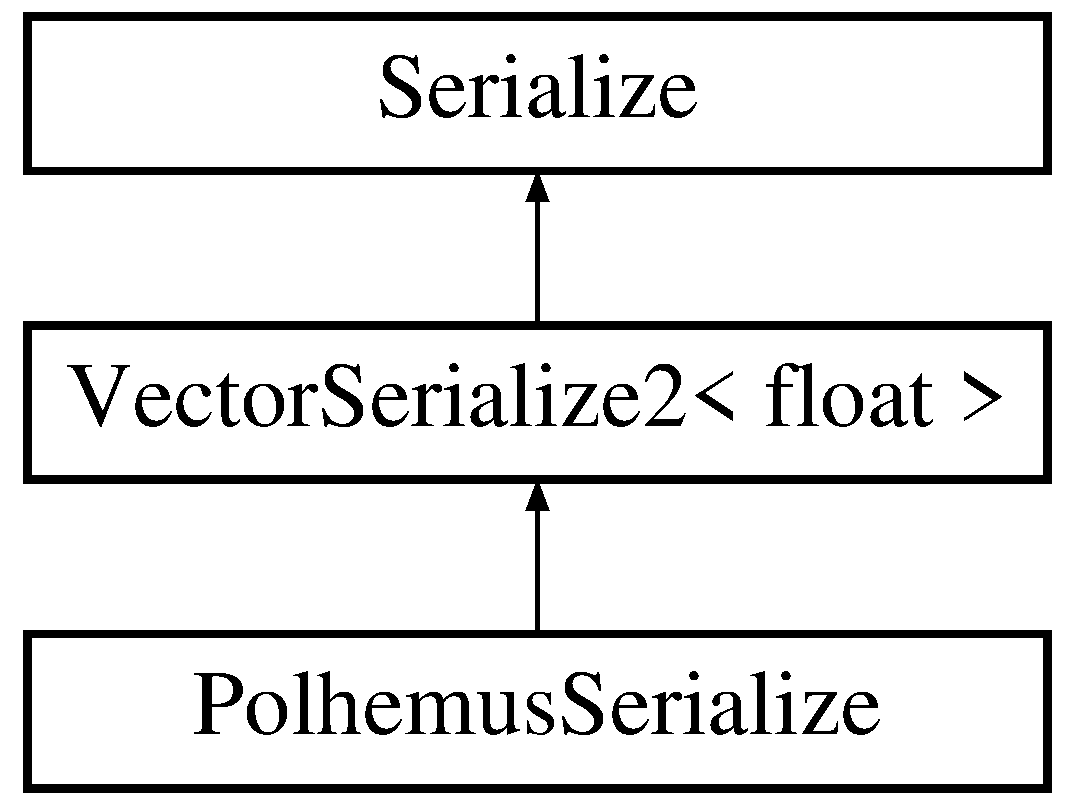
\includegraphics[height=3.000000cm]{classPolhemusSerialize}
\end{center}
\end{figure}
\subsection*{Public Member Functions}
\begin{DoxyCompactItemize}
\item 
\hyperlink{classPolhemusSerialize_ab302551eb8fc12cfda3af393a00ac63d}{Polhemus\-Serialize} (int nsensors)
\item 
\hyperlink{classPolhemusSerialize_a769685eca980416c300dccae33d7ebf7}{$\sim$\-Polhemus\-Serialize} ()
\item 
virtual bool \hyperlink{classPolhemusSerialize_a6cc3ac73da741cdeca76762ce991069c}{store} ()
\item 
bool \hyperlink{classPolhemusSerialize_a62051ba5f26905394ea7d0216cb0528f}{store} (float $\ast$data)
\item 
void \hyperlink{classPolhemusSerialize_ae973aa5770841739a7eb97a0d802f910}{get\-Loc} (double now, float $\ast$out)
\item 
virtual string \hyperlink{classPolhemusSerialize_a9f6cdf8427769c6e23ab2afc7cab07ce}{store\-Name} (int indx)
\item 
virtual double $\ast$ \hyperlink{classPolhemusSerialize_ac52dec8b5067a7f15a34c9e849be9eff}{mmap\-Read} (double $\ast$d)
\end{DoxyCompactItemize}
\subsection*{Public Attributes}
\begin{DoxyCompactItemize}
\item 
int \hyperlink{classPolhemusSerialize_a9cd18195743c2ac0a24f904dce28e1b8}{m\-\_\-nsensors}
\item 
vector$<$ \hyperlink{classPolhemusPredict}{Polhemus\-Predict} $\ast$ $>$ \hyperlink{classPolhemusSerialize_a07c4bd4c4bcf062c37954b5317608c0b}{m\-\_\-pp}
\end{DoxyCompactItemize}


\subsection{Constructor \& Destructor Documentation}
\hypertarget{classPolhemusSerialize_ab302551eb8fc12cfda3af393a00ac63d}{\index{Polhemus\-Serialize@{Polhemus\-Serialize}!Polhemus\-Serialize@{Polhemus\-Serialize}}
\index{Polhemus\-Serialize@{Polhemus\-Serialize}!PolhemusSerialize@{Polhemus\-Serialize}}
\subsubsection[{Polhemus\-Serialize}]{\setlength{\rightskip}{0pt plus 5cm}Polhemus\-Serialize\-::\-Polhemus\-Serialize (
\begin{DoxyParamCaption}
\item[{int}]{nsensors}
\end{DoxyParamCaption}
)}}\label{classPolhemusSerialize_ab302551eb8fc12cfda3af393a00ac63d}
\hypertarget{classPolhemusSerialize_a769685eca980416c300dccae33d7ebf7}{\index{Polhemus\-Serialize@{Polhemus\-Serialize}!$\sim$\-Polhemus\-Serialize@{$\sim$\-Polhemus\-Serialize}}
\index{$\sim$\-Polhemus\-Serialize@{$\sim$\-Polhemus\-Serialize}!PolhemusSerialize@{Polhemus\-Serialize}}
\subsubsection[{$\sim$\-Polhemus\-Serialize}]{\setlength{\rightskip}{0pt plus 5cm}Polhemus\-Serialize\-::$\sim$\-Polhemus\-Serialize (
\begin{DoxyParamCaption}
{}
\end{DoxyParamCaption}
)}}\label{classPolhemusSerialize_a769685eca980416c300dccae33d7ebf7}


\subsection{Member Function Documentation}
\hypertarget{classPolhemusSerialize_ae973aa5770841739a7eb97a0d802f910}{\index{Polhemus\-Serialize@{Polhemus\-Serialize}!get\-Loc@{get\-Loc}}
\index{get\-Loc@{get\-Loc}!PolhemusSerialize@{Polhemus\-Serialize}}
\subsubsection[{get\-Loc}]{\setlength{\rightskip}{0pt plus 5cm}void Polhemus\-Serialize\-::get\-Loc (
\begin{DoxyParamCaption}
\item[{double}]{now, }
\item[{float $\ast$}]{out}
\end{DoxyParamCaption}
)}}\label{classPolhemusSerialize_ae973aa5770841739a7eb97a0d802f910}
\hypertarget{classPolhemusSerialize_ac52dec8b5067a7f15a34c9e849be9eff}{\index{Polhemus\-Serialize@{Polhemus\-Serialize}!mmap\-Read@{mmap\-Read}}
\index{mmap\-Read@{mmap\-Read}!PolhemusSerialize@{Polhemus\-Serialize}}
\subsubsection[{mmap\-Read}]{\setlength{\rightskip}{0pt plus 5cm}double $\ast$ Polhemus\-Serialize\-::mmap\-Read (
\begin{DoxyParamCaption}
\item[{double $\ast$}]{d}
\end{DoxyParamCaption}
)\hspace{0.3cm}{\ttfamily [virtual]}}}\label{classPolhemusSerialize_ac52dec8b5067a7f15a34c9e849be9eff}


Reimplemented from \hyperlink{classVectorSerialize2_a8f4bf0a524b34b584d131b8fbfcd8d30}{Vector\-Serialize2$<$ float $>$}.

\hypertarget{classPolhemusSerialize_a6cc3ac73da741cdeca76762ce991069c}{\index{Polhemus\-Serialize@{Polhemus\-Serialize}!store@{store}}
\index{store@{store}!PolhemusSerialize@{Polhemus\-Serialize}}
\subsubsection[{store}]{\setlength{\rightskip}{0pt plus 5cm}bool Polhemus\-Serialize\-::store (
\begin{DoxyParamCaption}
{}
\end{DoxyParamCaption}
)\hspace{0.3cm}{\ttfamily [virtual]}}}\label{classPolhemusSerialize_a6cc3ac73da741cdeca76762ce991069c}


Reimplemented from \hyperlink{classVectorSerialize2_a720a62d5c2eb1299d445b35080662aaf}{Vector\-Serialize2$<$ float $>$}.

\hypertarget{classPolhemusSerialize_a62051ba5f26905394ea7d0216cb0528f}{\index{Polhemus\-Serialize@{Polhemus\-Serialize}!store@{store}}
\index{store@{store}!PolhemusSerialize@{Polhemus\-Serialize}}
\subsubsection[{store}]{\setlength{\rightskip}{0pt plus 5cm}bool Polhemus\-Serialize\-::store (
\begin{DoxyParamCaption}
\item[{float $\ast$}]{data}
\end{DoxyParamCaption}
)}}\label{classPolhemusSerialize_a62051ba5f26905394ea7d0216cb0528f}
\hypertarget{classPolhemusSerialize_a9f6cdf8427769c6e23ab2afc7cab07ce}{\index{Polhemus\-Serialize@{Polhemus\-Serialize}!store\-Name@{store\-Name}}
\index{store\-Name@{store\-Name}!PolhemusSerialize@{Polhemus\-Serialize}}
\subsubsection[{store\-Name}]{\setlength{\rightskip}{0pt plus 5cm}string Polhemus\-Serialize\-::store\-Name (
\begin{DoxyParamCaption}
\item[{int}]{indx}
\end{DoxyParamCaption}
)\hspace{0.3cm}{\ttfamily [virtual]}}}\label{classPolhemusSerialize_a9f6cdf8427769c6e23ab2afc7cab07ce}


Reimplemented from \hyperlink{classVectorSerialize2_ae0a636c3231b336b7dc8a9b2958b6b0e}{Vector\-Serialize2$<$ float $>$}.



\subsection{Member Data Documentation}
\hypertarget{classPolhemusSerialize_a9cd18195743c2ac0a24f904dce28e1b8}{\index{Polhemus\-Serialize@{Polhemus\-Serialize}!m\-\_\-nsensors@{m\-\_\-nsensors}}
\index{m\-\_\-nsensors@{m\-\_\-nsensors}!PolhemusSerialize@{Polhemus\-Serialize}}
\subsubsection[{m\-\_\-nsensors}]{\setlength{\rightskip}{0pt plus 5cm}int Polhemus\-Serialize\-::m\-\_\-nsensors}}\label{classPolhemusSerialize_a9cd18195743c2ac0a24f904dce28e1b8}
\hypertarget{classPolhemusSerialize_a07c4bd4c4bcf062c37954b5317608c0b}{\index{Polhemus\-Serialize@{Polhemus\-Serialize}!m\-\_\-pp@{m\-\_\-pp}}
\index{m\-\_\-pp@{m\-\_\-pp}!PolhemusSerialize@{Polhemus\-Serialize}}
\subsubsection[{m\-\_\-pp}]{\setlength{\rightskip}{0pt plus 5cm}vector$<${\bf Polhemus\-Predict} $\ast$$>$ Polhemus\-Serialize\-::m\-\_\-pp}}\label{classPolhemusSerialize_a07c4bd4c4bcf062c37954b5317608c0b}


The documentation for this class was generated from the following files\-:\begin{DoxyCompactItemize}
\item 
/home/ruijan/sw/bmi5/bmi5/include/\-Serialize/\hyperlink{polhemusSerialize_8h}{polhemus\-Serialize.\-h}\item 
/home/ruijan/sw/bmi5/bmi5/src/\-Serialize/\hyperlink{polhemusSerialize_8cpp}{polhemus\-Serialize.\-cpp}\end{DoxyCompactItemize}

\hypertarget{classRing}{\section{Ring Class Reference}
\label{classRing}\index{Ring@{Ring}}
}


{\ttfamily \#include $<$ring.\-h$>$}

Inheritance diagram for Ring\-:\begin{figure}[H]
\begin{center}
\leavevmode
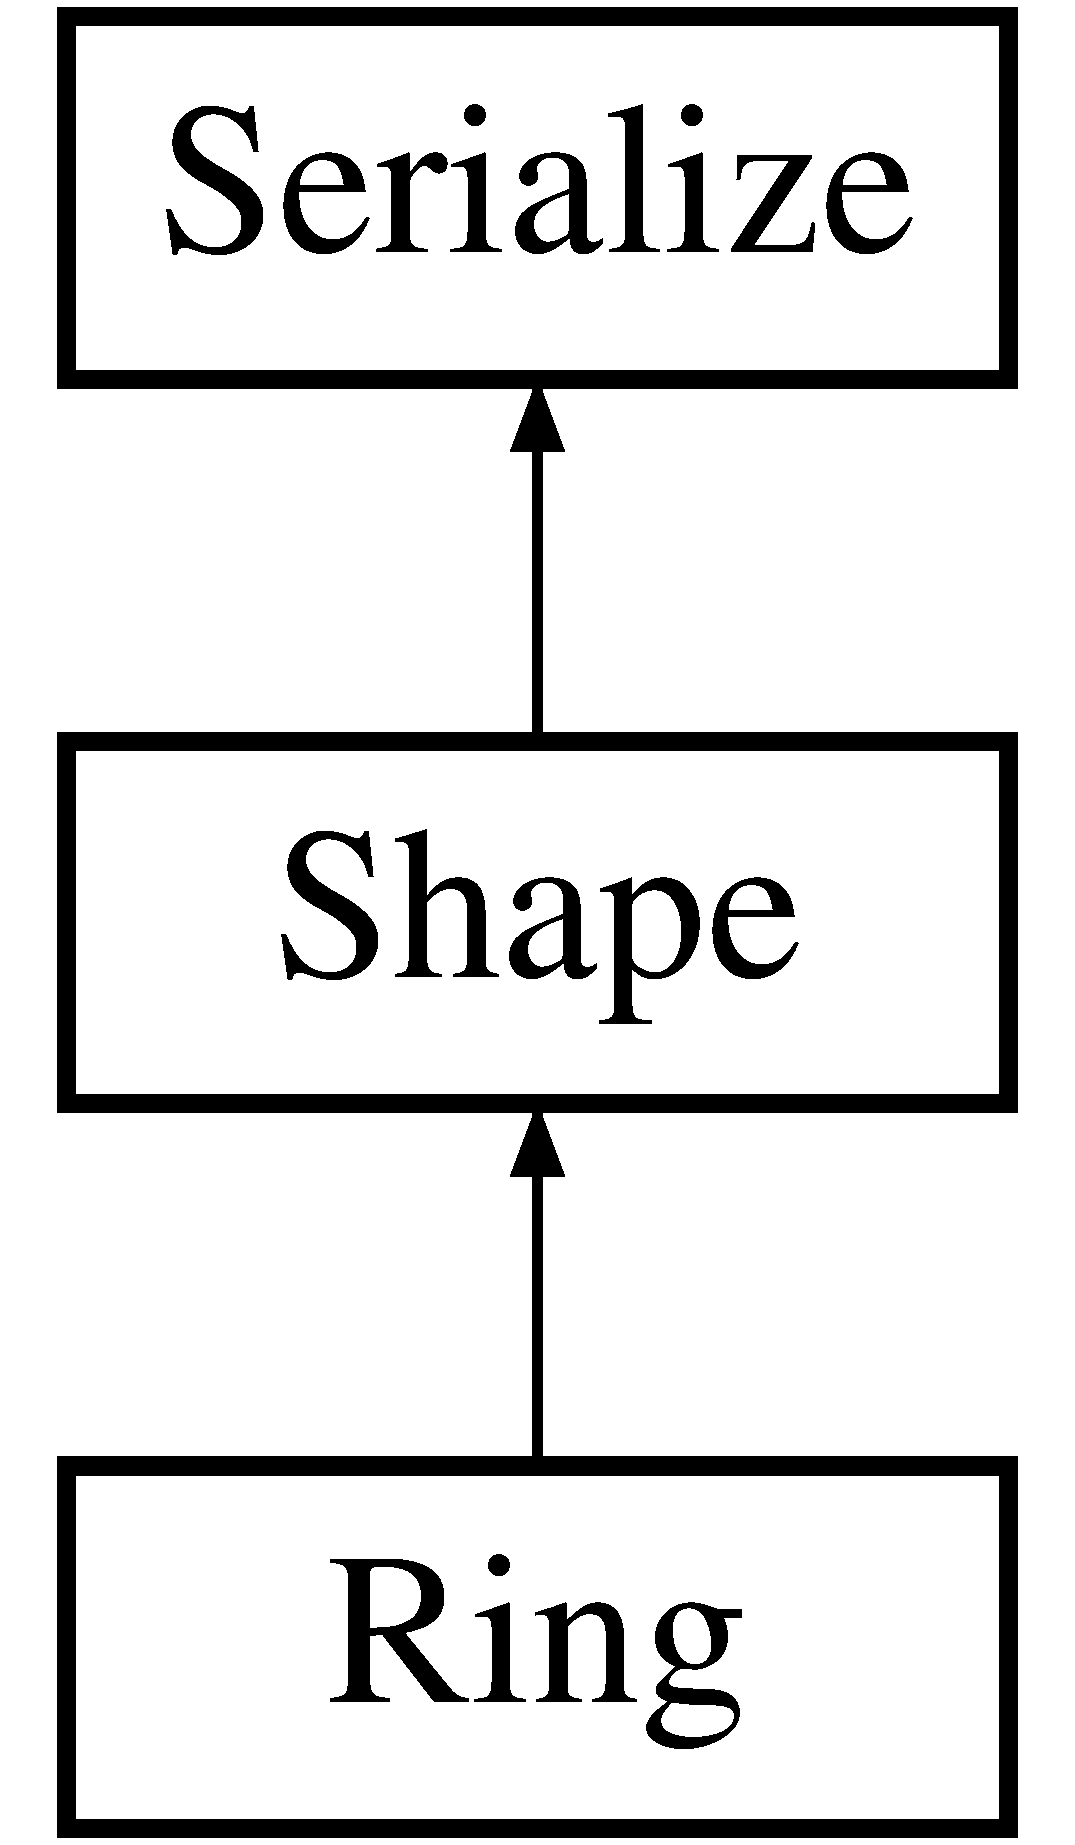
\includegraphics[height=3.000000cm]{classRing}
\end{center}
\end{figure}
\subsection*{Public Member Functions}
\begin{DoxyCompactItemize}
\item 
\hyperlink{classRing_a39d8bce00a532857c1f894355df655c1}{Ring} (float inner\-Radius, float outer\-Radius, int ns)
\item 
virtual \hyperlink{classRing_a515a41c0803bcdd921712d6f5047e101}{$\sim$\-Ring} ()
\item 
virtual void \hyperlink{classRing_ad5dd2b058f6690108fe62da9d6e88d53}{fill} (float $\ast$v)
\end{DoxyCompactItemize}
\subsection*{Private Attributes}
\begin{DoxyCompactItemize}
\item 
float \hyperlink{classRing_a5e4deb45ebf263e2a518d06df7f00afd}{m\-\_\-ir}
\item 
float \hyperlink{classRing_a4686fdcc73450cc4cb29dcd97908652c}{m\-\_\-or}
\item 
int \hyperlink{classRing_af2929b1d85186201b9325998d541d204}{m\-\_\-ns}
\end{DoxyCompactItemize}
\subsection*{Additional Inherited Members}


\subsection{Constructor \& Destructor Documentation}
\hypertarget{classRing_a39d8bce00a532857c1f894355df655c1}{\index{Ring@{Ring}!Ring@{Ring}}
\index{Ring@{Ring}!Ring@{Ring}}
\subsubsection[{Ring}]{\setlength{\rightskip}{0pt plus 5cm}Ring\-::\-Ring (
\begin{DoxyParamCaption}
\item[{float}]{inner\-Radius, }
\item[{float}]{outer\-Radius, }
\item[{int}]{ns}
\end{DoxyParamCaption}
)}}\label{classRing_a39d8bce00a532857c1f894355df655c1}
\hypertarget{classRing_a515a41c0803bcdd921712d6f5047e101}{\index{Ring@{Ring}!$\sim$\-Ring@{$\sim$\-Ring}}
\index{$\sim$\-Ring@{$\sim$\-Ring}!Ring@{Ring}}
\subsubsection[{$\sim$\-Ring}]{\setlength{\rightskip}{0pt plus 5cm}Ring\-::$\sim$\-Ring (
\begin{DoxyParamCaption}
{}
\end{DoxyParamCaption}
)\hspace{0.3cm}{\ttfamily [virtual]}}}\label{classRing_a515a41c0803bcdd921712d6f5047e101}


\subsection{Member Function Documentation}
\hypertarget{classRing_ad5dd2b058f6690108fe62da9d6e88d53}{\index{Ring@{Ring}!fill@{fill}}
\index{fill@{fill}!Ring@{Ring}}
\subsubsection[{fill}]{\setlength{\rightskip}{0pt plus 5cm}void Ring\-::fill (
\begin{DoxyParamCaption}
\item[{float $\ast$}]{v}
\end{DoxyParamCaption}
)\hspace{0.3cm}{\ttfamily [virtual]}}}\label{classRing_ad5dd2b058f6690108fe62da9d6e88d53}


Reimplemented from \hyperlink{classShape_a33be64d8e24518084b1c8f974f808387}{Shape}.



\subsection{Member Data Documentation}
\hypertarget{classRing_a5e4deb45ebf263e2a518d06df7f00afd}{\index{Ring@{Ring}!m\-\_\-ir@{m\-\_\-ir}}
\index{m\-\_\-ir@{m\-\_\-ir}!Ring@{Ring}}
\subsubsection[{m\-\_\-ir}]{\setlength{\rightskip}{0pt plus 5cm}float Ring\-::m\-\_\-ir\hspace{0.3cm}{\ttfamily [private]}}}\label{classRing_a5e4deb45ebf263e2a518d06df7f00afd}
\hypertarget{classRing_af2929b1d85186201b9325998d541d204}{\index{Ring@{Ring}!m\-\_\-ns@{m\-\_\-ns}}
\index{m\-\_\-ns@{m\-\_\-ns}!Ring@{Ring}}
\subsubsection[{m\-\_\-ns}]{\setlength{\rightskip}{0pt plus 5cm}int Ring\-::m\-\_\-ns\hspace{0.3cm}{\ttfamily [private]}}}\label{classRing_af2929b1d85186201b9325998d541d204}
\hypertarget{classRing_a4686fdcc73450cc4cb29dcd97908652c}{\index{Ring@{Ring}!m\-\_\-or@{m\-\_\-or}}
\index{m\-\_\-or@{m\-\_\-or}!Ring@{Ring}}
\subsubsection[{m\-\_\-or}]{\setlength{\rightskip}{0pt plus 5cm}float Ring\-::m\-\_\-or\hspace{0.3cm}{\ttfamily [private]}}}\label{classRing_a4686fdcc73450cc4cb29dcd97908652c}


The documentation for this class was generated from the following files\-:\begin{DoxyCompactItemize}
\item 
/home/ruijan/sw/bmi5/bmi5/include/\-Shape/\hyperlink{ring_8h}{ring.\-h}\item 
/home/ruijan/sw/bmi5/bmi5/src/\-Shape/\hyperlink{ring_8cpp}{ring.\-cpp}\end{DoxyCompactItemize}

\hypertarget{classSerialize}{\section{Serialize Class Reference}
\label{classSerialize}\index{Serialize@{Serialize}}
}


{\ttfamily \#include $<$serialize.\-h$>$}

Inheritance diagram for Serialize\-:\begin{figure}[H]
\begin{center}
\leavevmode
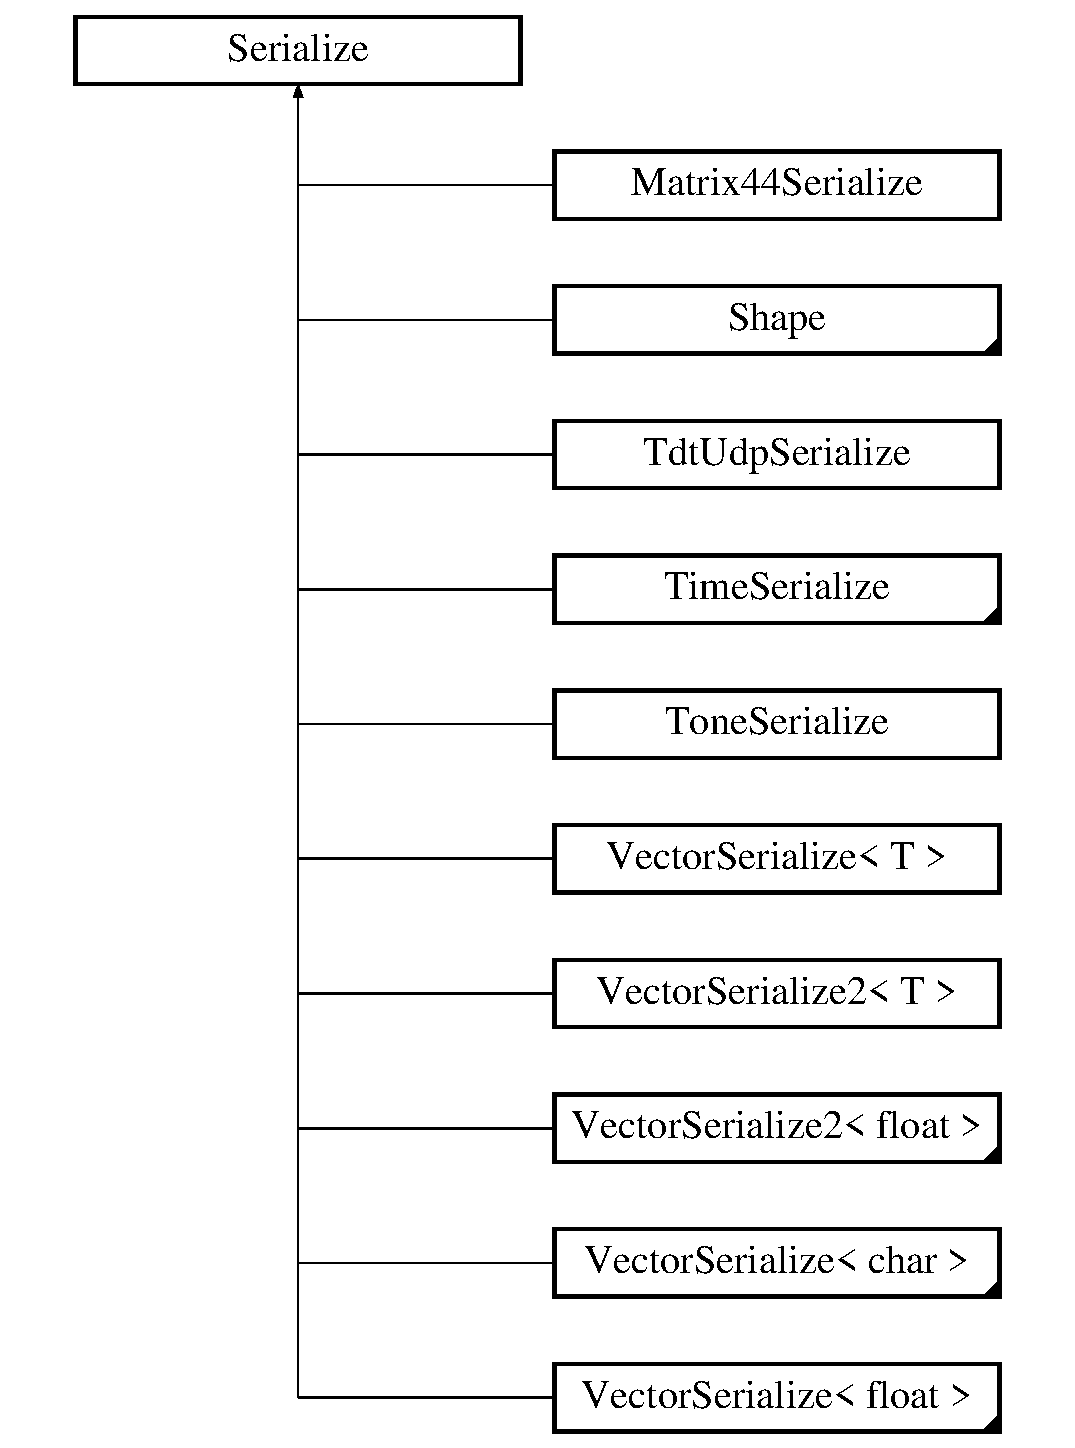
\includegraphics[height=11.000000cm]{classSerialize}
\end{center}
\end{figure}
\subsection*{Public Member Functions}
\begin{DoxyCompactItemize}
\item 
\hyperlink{classSerialize_ab594f8f89b0be6b0c1439516a01fc7f7}{Serialize} ()
\item 
virtual \hyperlink{classSerialize_a44999f67289d084f299ac0e9cfb1135d}{$\sim$\-Serialize} ()
\item 
void \hyperlink{classSerialize_aabbc8730e307d42c99741443c036ca97}{perr} (const char $\ast$method)
\item 
virtual bool \hyperlink{classSerialize_a3cda20e84a530870a6115eaaf589f168}{store} ()
\item 
virtual void \hyperlink{classSerialize_a11cbf006415c08d1891ab42e39a2aa1a}{clear} ()
\item 
virtual int \hyperlink{classSerialize_a590b7308112b07581c03ba826ace50b4}{nstored} ()
\item 
virtual string \hyperlink{classSerialize_ac94a76de6c9376e33b4c195d50ff0568}{store\-Name} (int)
\item 
virtual int \hyperlink{classSerialize_a69954cc86d03b75b6b27511aec4aba43}{get\-Store\-Class} (int)
\item 
virtual void \hyperlink{classSerialize_a52034c5c17bc5e7e6c728b4e6c620c05}{get\-Store\-Dims} (int, size\-\_\-t $\ast$dims)
\item 
virtual void $\ast$ \hyperlink{classSerialize_a6e589d263cfdc0eb72e41687c58831f2}{get\-Store} (int, int)
\item 
virtual int \hyperlink{classSerialize_a71bf2a906fd71477308a942d01490ab3}{num\-Stores} ()
\item 
virtual double $\ast$ \hyperlink{classSerialize_a28b939242880e565a8906b30acd0f84c}{mmap\-Read} (double $\ast$)
\item 
virtual void \hyperlink{classSerialize_a0cf1d14e41052c6eabe53c90a37c227b}{draw} (int, float)
\item 
virtual void \hyperlink{classSerialize_a06cf228664e659c8490c63ee36f34e28}{move} (long double)
\item 
virtual string \hyperlink{classSerialize_a0100618d428589974b6b80d4232e91ff}{get\-Mmap\-Info} ()
\item 
virtual string \hyperlink{classSerialize_a343c898670261dc23b955127de1574cd}{get\-Struct\-Info} ()
\end{DoxyCompactItemize}
\subsection*{Public Attributes}
\begin{DoxyCompactItemize}
\item 
string \hyperlink{classSerialize_a9fdb3475fed69e393e8421a21a22a241}{m\-\_\-name}
\item 
int \hyperlink{classSerialize_a011cc1272d6018ef424f11b33b652019}{m\-\_\-last\-Backup}
\end{DoxyCompactItemize}


\subsection{Constructor \& Destructor Documentation}
\hypertarget{classSerialize_ab594f8f89b0be6b0c1439516a01fc7f7}{\index{Serialize@{Serialize}!Serialize@{Serialize}}
\index{Serialize@{Serialize}!Serialize@{Serialize}}
\subsubsection[{Serialize}]{\setlength{\rightskip}{0pt plus 5cm}Serialize\-::\-Serialize (
\begin{DoxyParamCaption}
{}
\end{DoxyParamCaption}
)}}\label{classSerialize_ab594f8f89b0be6b0c1439516a01fc7f7}
\hypertarget{classSerialize_a44999f67289d084f299ac0e9cfb1135d}{\index{Serialize@{Serialize}!$\sim$\-Serialize@{$\sim$\-Serialize}}
\index{$\sim$\-Serialize@{$\sim$\-Serialize}!Serialize@{Serialize}}
\subsubsection[{$\sim$\-Serialize}]{\setlength{\rightskip}{0pt plus 5cm}Serialize\-::$\sim$\-Serialize (
\begin{DoxyParamCaption}
{}
\end{DoxyParamCaption}
)\hspace{0.3cm}{\ttfamily [virtual]}}}\label{classSerialize_a44999f67289d084f299ac0e9cfb1135d}


\subsection{Member Function Documentation}
\hypertarget{classSerialize_a11cbf006415c08d1891ab42e39a2aa1a}{\index{Serialize@{Serialize}!clear@{clear}}
\index{clear@{clear}!Serialize@{Serialize}}
\subsubsection[{clear}]{\setlength{\rightskip}{0pt plus 5cm}void Serialize\-::clear (
\begin{DoxyParamCaption}
{}
\end{DoxyParamCaption}
)\hspace{0.3cm}{\ttfamily [virtual]}}}\label{classSerialize_a11cbf006415c08d1891ab42e39a2aa1a}


Reimplemented in \hyperlink{classShape_afc0a792fc9c31a0ae947f721c146f68b}{Shape}, \hyperlink{classStarField_a1a97b6133ae0177f6eb8028470c28765}{Star\-Field}, \hyperlink{classVectorSerialize_ae94606fef7aec9ade8142d3cd56449ab}{Vector\-Serialize$<$ T $>$}, \hyperlink{classVectorSerialize2_ae8029b8225cbc4f9e07051949563e473}{Vector\-Serialize2$<$ T $>$}, \hyperlink{classVectorSerialize_ae94606fef7aec9ade8142d3cd56449ab}{Vector\-Serialize$<$ float $>$}, \hyperlink{classVectorSerialize_ae94606fef7aec9ade8142d3cd56449ab}{Vector\-Serialize$<$ char $>$}, \hyperlink{classVectorSerialize2_ae8029b8225cbc4f9e07051949563e473}{Vector\-Serialize2$<$ float $>$}, \hyperlink{classTdtUdpSerialize_ac8510f3a23c5521f819c328d9e49bce7}{Tdt\-Udp\-Serialize}, \hyperlink{classDisplayText_a0c7a7a5200482ea4817f6c550dc7dea9}{Display\-Text}, \hyperlink{classToneSerialize_a1670e9459e05b63f1b6fff4d6ff13099}{Tone\-Serialize}, \hyperlink{classTimeSerialize_a2dc0323aaec9735cec278fce2ab70779}{Time\-Serialize}, and \hyperlink{classMatrix44Serialize_aaea63fa835d82cc7d039323e678ec58a}{Matrix44\-Serialize}.

\hypertarget{classSerialize_a0cf1d14e41052c6eabe53c90a37c227b}{\index{Serialize@{Serialize}!draw@{draw}}
\index{draw@{draw}!Serialize@{Serialize}}
\subsubsection[{draw}]{\setlength{\rightskip}{0pt plus 5cm}void Serialize\-::draw (
\begin{DoxyParamCaption}
\item[{int}]{, }
\item[{float}]{}
\end{DoxyParamCaption}
)\hspace{0.3cm}{\ttfamily [virtual]}}}\label{classSerialize_a0cf1d14e41052c6eabe53c90a37c227b}


Reimplemented in \hyperlink{classShape_a892243993a2207807ab5069ce90bbef4}{Shape}, \hyperlink{classStarField_aeaf743e6d1d4a8a6918152c40bd618c0}{Star\-Field}, and \hyperlink{classDisplayText_a1eddd0c9f33244eb10540c51aa1dbfda}{Display\-Text}.

\hypertarget{classSerialize_a0100618d428589974b6b80d4232e91ff}{\index{Serialize@{Serialize}!get\-Mmap\-Info@{get\-Mmap\-Info}}
\index{get\-Mmap\-Info@{get\-Mmap\-Info}!Serialize@{Serialize}}
\subsubsection[{get\-Mmap\-Info}]{\setlength{\rightskip}{0pt plus 5cm}string Serialize\-::get\-Mmap\-Info (
\begin{DoxyParamCaption}
{}
\end{DoxyParamCaption}
)\hspace{0.3cm}{\ttfamily [virtual]}}}\label{classSerialize_a0100618d428589974b6b80d4232e91ff}
\hypertarget{classSerialize_a6e589d263cfdc0eb72e41687c58831f2}{\index{Serialize@{Serialize}!get\-Store@{get\-Store}}
\index{get\-Store@{get\-Store}!Serialize@{Serialize}}
\subsubsection[{get\-Store}]{\setlength{\rightskip}{0pt plus 5cm}void $\ast$ Serialize\-::get\-Store (
\begin{DoxyParamCaption}
\item[{int}]{, }
\item[{int}]{}
\end{DoxyParamCaption}
)\hspace{0.3cm}{\ttfamily [virtual]}}}\label{classSerialize_a6e589d263cfdc0eb72e41687c58831f2}


Reimplemented in \hyperlink{classShape_ae89da51d3c54b7b7139b8223103633e3}{Shape}, \hyperlink{classStarField_a3d33db9d5e4c05a11cbe0c11a3bae5ba}{Star\-Field}, \hyperlink{classVectorSerialize_a08f1412b11fb7b034da21c5ec131489b}{Vector\-Serialize$<$ T $>$}, \hyperlink{classVectorSerialize2_a856c33259537f46fe8c579bd6532a3f4}{Vector\-Serialize2$<$ T $>$}, \hyperlink{classVectorSerialize_a08f1412b11fb7b034da21c5ec131489b}{Vector\-Serialize$<$ float $>$}, \hyperlink{classVectorSerialize_a08f1412b11fb7b034da21c5ec131489b}{Vector\-Serialize$<$ char $>$}, \hyperlink{classVectorSerialize2_a856c33259537f46fe8c579bd6532a3f4}{Vector\-Serialize2$<$ float $>$}, \hyperlink{classTdtUdpSerialize_ae46b100495af52e51be07ed2df3e76d7}{Tdt\-Udp\-Serialize}, \hyperlink{classToneSerialize_a6999157d41af65a3b7e8ea101972fd4e}{Tone\-Serialize}, \hyperlink{classDisplayText_aea5003c9c461955ec3c9a3a4b4fc2c25}{Display\-Text}, \hyperlink{classTimeSerialize_aca830871918f9acf615366df5e1eeb11}{Time\-Serialize}, and \hyperlink{classMatrix44Serialize_a4690b73080db8812c3ca0970f05c699d}{Matrix44\-Serialize}.

\hypertarget{classSerialize_a69954cc86d03b75b6b27511aec4aba43}{\index{Serialize@{Serialize}!get\-Store\-Class@{get\-Store\-Class}}
\index{get\-Store\-Class@{get\-Store\-Class}!Serialize@{Serialize}}
\subsubsection[{get\-Store\-Class}]{\setlength{\rightskip}{0pt plus 5cm}int Serialize\-::get\-Store\-Class (
\begin{DoxyParamCaption}
\item[{int}]{}
\end{DoxyParamCaption}
)\hspace{0.3cm}{\ttfamily [virtual]}}}\label{classSerialize_a69954cc86d03b75b6b27511aec4aba43}


Reimplemented in \hyperlink{classShape_acf135c0569e45aa0fab16f748bee639e}{Shape}, \hyperlink{classStarField_a42fa7234a0bb1e7b2e1d734fb9ed2dae}{Star\-Field}, \hyperlink{classVectorSerialize_a03d8454fff77942e63cd1764f1013f2d}{Vector\-Serialize$<$ T $>$}, \hyperlink{classVectorSerialize2_acc7178f7f25ba6c275041a0e530befdb}{Vector\-Serialize2$<$ T $>$}, \hyperlink{classVectorSerialize_a03d8454fff77942e63cd1764f1013f2d}{Vector\-Serialize$<$ float $>$}, \hyperlink{classVectorSerialize_a03d8454fff77942e63cd1764f1013f2d}{Vector\-Serialize$<$ char $>$}, \hyperlink{classVectorSerialize2_acc7178f7f25ba6c275041a0e530befdb}{Vector\-Serialize2$<$ float $>$}, \hyperlink{classTdtUdpSerialize_a9dd4bd127aa84ce5aa4440a4e6f2f1ce}{Tdt\-Udp\-Serialize}, \hyperlink{classToneSerialize_a651a5292dabf70de6f562695ca034d8d}{Tone\-Serialize}, \hyperlink{classDisplayText_aaa8ccb67b152d79505e5acc8448770ed}{Display\-Text}, \hyperlink{classTimeSerialize_aabe62de35575d2e543c1b6a60adee905}{Time\-Serialize}, and \hyperlink{classMatrix44Serialize_a543c479bc5f47c7045988f14dc398cfa}{Matrix44\-Serialize}.

\hypertarget{classSerialize_a52034c5c17bc5e7e6c728b4e6c620c05}{\index{Serialize@{Serialize}!get\-Store\-Dims@{get\-Store\-Dims}}
\index{get\-Store\-Dims@{get\-Store\-Dims}!Serialize@{Serialize}}
\subsubsection[{get\-Store\-Dims}]{\setlength{\rightskip}{0pt plus 5cm}void Serialize\-::get\-Store\-Dims (
\begin{DoxyParamCaption}
\item[{int}]{, }
\item[{size\-\_\-t $\ast$}]{dims}
\end{DoxyParamCaption}
)\hspace{0.3cm}{\ttfamily [virtual]}}}\label{classSerialize_a52034c5c17bc5e7e6c728b4e6c620c05}


Reimplemented in \hyperlink{classShape_afc3fbc26459718484ae4efe885f0fe37}{Shape}, \hyperlink{classStarField_a1cf58acb059f13adcb4b989120f99db5}{Star\-Field}, \hyperlink{classVectorSerialize_aa22f90d57d8802670716f4b859d6b069}{Vector\-Serialize$<$ T $>$}, \hyperlink{classVectorSerialize2_a0377d72ce381217f8e8d250509226aec}{Vector\-Serialize2$<$ T $>$}, \hyperlink{classVectorSerialize_aa22f90d57d8802670716f4b859d6b069}{Vector\-Serialize$<$ float $>$}, \hyperlink{classVectorSerialize_aa22f90d57d8802670716f4b859d6b069}{Vector\-Serialize$<$ char $>$}, \hyperlink{classVectorSerialize2_a0377d72ce381217f8e8d250509226aec}{Vector\-Serialize2$<$ float $>$}, \hyperlink{classTdtUdpSerialize_a1ef45e16bef8085e38796f0e94bc8333}{Tdt\-Udp\-Serialize}, \hyperlink{classToneSerialize_a3756f8357f284843aeaa5c56f98ff5db}{Tone\-Serialize}, \hyperlink{classDisplayText_a81a37dd4e0fa54265843db620c371d02}{Display\-Text}, \hyperlink{classTimeSerialize_a012cef4eb5d7766296987d57dcd7b6d1}{Time\-Serialize}, and \hyperlink{classMatrix44Serialize_ad2a049be2ae27daad403c7e1d7ca4de0}{Matrix44\-Serialize}.

\hypertarget{classSerialize_a343c898670261dc23b955127de1574cd}{\index{Serialize@{Serialize}!get\-Struct\-Info@{get\-Struct\-Info}}
\index{get\-Struct\-Info@{get\-Struct\-Info}!Serialize@{Serialize}}
\subsubsection[{get\-Struct\-Info}]{\setlength{\rightskip}{0pt plus 5cm}string Serialize\-::get\-Struct\-Info (
\begin{DoxyParamCaption}
{}
\end{DoxyParamCaption}
)\hspace{0.3cm}{\ttfamily [virtual]}}}\label{classSerialize_a343c898670261dc23b955127de1574cd}
\hypertarget{classSerialize_a28b939242880e565a8906b30acd0f84c}{\index{Serialize@{Serialize}!mmap\-Read@{mmap\-Read}}
\index{mmap\-Read@{mmap\-Read}!Serialize@{Serialize}}
\subsubsection[{mmap\-Read}]{\setlength{\rightskip}{0pt plus 5cm}double $\ast$ Serialize\-::mmap\-Read (
\begin{DoxyParamCaption}
\item[{double $\ast$}]{}
\end{DoxyParamCaption}
)\hspace{0.3cm}{\ttfamily [virtual]}}}\label{classSerialize_a28b939242880e565a8906b30acd0f84c}


Reimplemented in \hyperlink{classShape_ae212539c5d1468805c155f4aed8367ea}{Shape}, \hyperlink{classStarField_a6937d614690f774772920ae9faee9bab}{Star\-Field}, \hyperlink{classVectorSerialize_a087c30b15095d1b230705e42123eb3db}{Vector\-Serialize$<$ T $>$}, \hyperlink{classVectorSerialize2_a8f4bf0a524b34b584d131b8fbfcd8d30}{Vector\-Serialize2$<$ T $>$}, \hyperlink{classVectorSerialize_a087c30b15095d1b230705e42123eb3db}{Vector\-Serialize$<$ float $>$}, \hyperlink{classVectorSerialize_a087c30b15095d1b230705e42123eb3db}{Vector\-Serialize$<$ char $>$}, \hyperlink{classVectorSerialize2_a8f4bf0a524b34b584d131b8fbfcd8d30}{Vector\-Serialize2$<$ float $>$}, \hyperlink{classTdtUdpSerialize_ad22fb90570005daa6e8768c2f5dbb531}{Tdt\-Udp\-Serialize}, \hyperlink{classToneSerialize_adaf612569b11204b02fc3393b780f75e}{Tone\-Serialize}, \hyperlink{classDisplayText_ae5f08045997631736d8400ad3662fe5b}{Display\-Text}, \hyperlink{classTimeSerialize_ac7a17bf484eb4e7970532b6a1ed65325}{Time\-Serialize}, \hyperlink{classMatrix44Serialize_a9882ee2bdc032d63cc2daf6eb25a7464}{Matrix44\-Serialize}, \hyperlink{classPolhemusSerialize_ac52dec8b5067a7f15a34c9e849be9eff}{Polhemus\-Serialize}, \hyperlink{classOptoSerialize_a35e6ee49e354276af9548a759fa3f3d2}{Opto\-Serialize}, \hyperlink{classFrameSerialize_a9d775f9c379f0444a82cd309bba9e9b1}{Frame\-Serialize}, \hyperlink{classLabjackSerializeAIN_a5b64792931481c509eb0c2bb86dbc99a}{Labjack\-Serialize\-A\-I\-N}, \hyperlink{classLabjackSerializeDOUT_a8936d25baa4652bb431b02ccb60489be}{Labjack\-Serialize\-D\-O\-U\-T}, and \hyperlink{classMouseSerialize_ab919e98d4daf8a068fc68741a4a4dcb7}{Mouse\-Serialize}.

\hypertarget{classSerialize_a06cf228664e659c8490c63ee36f34e28}{\index{Serialize@{Serialize}!move@{move}}
\index{move@{move}!Serialize@{Serialize}}
\subsubsection[{move}]{\setlength{\rightskip}{0pt plus 5cm}void Serialize\-::move (
\begin{DoxyParamCaption}
\item[{long double}]{}
\end{DoxyParamCaption}
)\hspace{0.3cm}{\ttfamily [virtual]}}}\label{classSerialize_a06cf228664e659c8490c63ee36f34e28}


Reimplemented in \hyperlink{classShape_ac39d8d75d7498e3cd5395b8485fbf39f}{Shape}, \hyperlink{classStarField_ac3e35d838577ed7610bdaf933ef5b99d}{Star\-Field}, and \hyperlink{classStarFieldCircle_af54e17032bb1ee195137b3585e7caea5}{Star\-Field\-Circle}.

\hypertarget{classSerialize_a590b7308112b07581c03ba826ace50b4}{\index{Serialize@{Serialize}!nstored@{nstored}}
\index{nstored@{nstored}!Serialize@{Serialize}}
\subsubsection[{nstored}]{\setlength{\rightskip}{0pt plus 5cm}int Serialize\-::nstored (
\begin{DoxyParamCaption}
{}
\end{DoxyParamCaption}
)\hspace{0.3cm}{\ttfamily [virtual]}}}\label{classSerialize_a590b7308112b07581c03ba826ace50b4}


Reimplemented in \hyperlink{classShape_a92f5bc7b0179d1c47c2ae916727bf73d}{Shape}, \hyperlink{classVectorSerialize_a97c0db5a4da6c14c9c053092cc89e2bd}{Vector\-Serialize$<$ T $>$}, \hyperlink{classVectorSerialize2_ab73b56a93e5d7ebba81727a16a5f2179}{Vector\-Serialize2$<$ T $>$}, \hyperlink{classVectorSerialize_a97c0db5a4da6c14c9c053092cc89e2bd}{Vector\-Serialize$<$ float $>$}, \hyperlink{classVectorSerialize_a97c0db5a4da6c14c9c053092cc89e2bd}{Vector\-Serialize$<$ char $>$}, \hyperlink{classVectorSerialize2_ab73b56a93e5d7ebba81727a16a5f2179}{Vector\-Serialize2$<$ float $>$}, \hyperlink{classTdtUdpSerialize_a08a3fcd343162a03108e49e258a5faab}{Tdt\-Udp\-Serialize}, \hyperlink{classToneSerialize_a6a5a872eb9e1a282c0de2221c777c144}{Tone\-Serialize}, \hyperlink{classTimeSerialize_a8decf0dd155f7c185d5ed4a96ad8df6e}{Time\-Serialize}, and \hyperlink{classMatrix44Serialize_ab1531b0cb71530688376e3b5f9e05076}{Matrix44\-Serialize}.

\hypertarget{classSerialize_a71bf2a906fd71477308a942d01490ab3}{\index{Serialize@{Serialize}!num\-Stores@{num\-Stores}}
\index{num\-Stores@{num\-Stores}!Serialize@{Serialize}}
\subsubsection[{num\-Stores}]{\setlength{\rightskip}{0pt plus 5cm}int Serialize\-::num\-Stores (
\begin{DoxyParamCaption}
{}
\end{DoxyParamCaption}
)\hspace{0.3cm}{\ttfamily [virtual]}}}\label{classSerialize_a71bf2a906fd71477308a942d01490ab3}


Reimplemented in \hyperlink{classShape_a53bac379f3ad1537e56625015afd5c95}{Shape}, \hyperlink{classStarField_a1289224a6763a69ac041eb32d685b657}{Star\-Field}, \hyperlink{classVectorSerialize_a15226c69bda0fff870f20026f8681d80}{Vector\-Serialize$<$ T $>$}, \hyperlink{classVectorSerialize2_a79c978e6e087c1e7bc398f678d2e943f}{Vector\-Serialize2$<$ T $>$}, \hyperlink{classVectorSerialize_a15226c69bda0fff870f20026f8681d80}{Vector\-Serialize$<$ float $>$}, \hyperlink{classVectorSerialize_a15226c69bda0fff870f20026f8681d80}{Vector\-Serialize$<$ char $>$}, \hyperlink{classVectorSerialize2_a79c978e6e087c1e7bc398f678d2e943f}{Vector\-Serialize2$<$ float $>$}, \hyperlink{classTdtUdpSerialize_a20d01c52f776c41002502949aae53896}{Tdt\-Udp\-Serialize}, \hyperlink{classToneSerialize_a85f4bff56b0f43466079c2ff289aa03a}{Tone\-Serialize}, \hyperlink{classDisplayText_a06b49281616900153577f7c731e4bd62}{Display\-Text}, \hyperlink{classTimeSerialize_af36ff5a97baec0656b91373b72796a5f}{Time\-Serialize}, and \hyperlink{classMatrix44Serialize_aa87157b168588ba1e29d6dee6529e906}{Matrix44\-Serialize}.

\hypertarget{classSerialize_aabbc8730e307d42c99741443c036ca97}{\index{Serialize@{Serialize}!perr@{perr}}
\index{perr@{perr}!Serialize@{Serialize}}
\subsubsection[{perr}]{\setlength{\rightskip}{0pt plus 5cm}void Serialize\-::perr (
\begin{DoxyParamCaption}
\item[{const char $\ast$}]{method}
\end{DoxyParamCaption}
)}}\label{classSerialize_aabbc8730e307d42c99741443c036ca97}
\hypertarget{classSerialize_a3cda20e84a530870a6115eaaf589f168}{\index{Serialize@{Serialize}!store@{store}}
\index{store@{store}!Serialize@{Serialize}}
\subsubsection[{store}]{\setlength{\rightskip}{0pt plus 5cm}bool Serialize\-::store (
\begin{DoxyParamCaption}
{}
\end{DoxyParamCaption}
)\hspace{0.3cm}{\ttfamily [virtual]}}}\label{classSerialize_a3cda20e84a530870a6115eaaf589f168}


Reimplemented in \hyperlink{classShape_a9dea3f39fe203b2f4288dc7cda6295a7}{Shape}, \hyperlink{classStarField_aa8411004d05d05ac3e0f8d10bfa1949e}{Star\-Field}, \hyperlink{classVectorSerialize_afd6b6dc8768969dae5f27f46eeab83e6}{Vector\-Serialize$<$ T $>$}, \hyperlink{classVectorSerialize2_a720a62d5c2eb1299d445b35080662aaf}{Vector\-Serialize2$<$ T $>$}, \hyperlink{classVectorSerialize_afd6b6dc8768969dae5f27f46eeab83e6}{Vector\-Serialize$<$ float $>$}, \hyperlink{classVectorSerialize_afd6b6dc8768969dae5f27f46eeab83e6}{Vector\-Serialize$<$ char $>$}, \hyperlink{classVectorSerialize2_a720a62d5c2eb1299d445b35080662aaf}{Vector\-Serialize2$<$ float $>$}, \hyperlink{classTdtUdpSerialize_af90b9dd030658a60dd7221b68e47b0c1}{Tdt\-Udp\-Serialize}, \hyperlink{classDisplayText_a16d096c25b729eabfce141eb7dcf9012}{Display\-Text}, \hyperlink{classPolhemusSerialize_a6cc3ac73da741cdeca76762ce991069c}{Polhemus\-Serialize}, \hyperlink{classToneSerialize_ab67181fa3c51dded04a2d8b4fc55edb4}{Tone\-Serialize}, \hyperlink{classFrameSerialize_a5c2bbf78b071f73554611b82ad395573}{Frame\-Serialize}, \hyperlink{classMatrix44Serialize_a96da5f524e0e2522085f82b20f6e3de0}{Matrix44\-Serialize}, \hyperlink{classOptoSerialize_aef848193a25e0b103e31f8d25035af16}{Opto\-Serialize}, \hyperlink{classTimeSerialize_a5fa3f8491cf69cafb608ed06d16b744b}{Time\-Serialize}, \hyperlink{classLabjackSerializeDOUT_a2f896d9076b742cbc6fb58faf7cc7b91}{Labjack\-Serialize\-D\-O\-U\-T}, \hyperlink{classLabjackSerializeAIN_a12e5f38cd48f38578f46e8cc90576a93}{Labjack\-Serialize\-A\-I\-N}, and \hyperlink{classMouseSerialize_acfe8874b5ea2c2e4a2f235b7b97780e8}{Mouse\-Serialize}.

\hypertarget{classSerialize_ac94a76de6c9376e33b4c195d50ff0568}{\index{Serialize@{Serialize}!store\-Name@{store\-Name}}
\index{store\-Name@{store\-Name}!Serialize@{Serialize}}
\subsubsection[{store\-Name}]{\setlength{\rightskip}{0pt plus 5cm}string Serialize\-::store\-Name (
\begin{DoxyParamCaption}
\item[{int}]{}
\end{DoxyParamCaption}
)\hspace{0.3cm}{\ttfamily [virtual]}}}\label{classSerialize_ac94a76de6c9376e33b4c195d50ff0568}


Reimplemented in \hyperlink{classShape_aaf3b0b140fcaf0bb11c28493ef745bfd}{Shape}, \hyperlink{classStarField_a047f987e052fc14fd8041658c153e0f1}{Star\-Field}, \hyperlink{classVectorSerialize_a929f94f68d0a99c61308520a679ae1a2}{Vector\-Serialize$<$ T $>$}, \hyperlink{classVectorSerialize2_ae0a636c3231b336b7dc8a9b2958b6b0e}{Vector\-Serialize2$<$ T $>$}, \hyperlink{classVectorSerialize_a929f94f68d0a99c61308520a679ae1a2}{Vector\-Serialize$<$ float $>$}, \hyperlink{classVectorSerialize_a929f94f68d0a99c61308520a679ae1a2}{Vector\-Serialize$<$ char $>$}, \hyperlink{classVectorSerialize2_ae0a636c3231b336b7dc8a9b2958b6b0e}{Vector\-Serialize2$<$ float $>$}, \hyperlink{classTdtUdpSerialize_aadd92c08f9323862f7f166a9e2cfaa83}{Tdt\-Udp\-Serialize}, \hyperlink{classPolhemusSerialize_a9f6cdf8427769c6e23ab2afc7cab07ce}{Polhemus\-Serialize}, \hyperlink{classToneSerialize_a4ae952e04b0a89ba3d5a8cb82460b064}{Tone\-Serialize}, \hyperlink{classDisplayText_af663118f6d5010d2d1d45f2bf3680dfc}{Display\-Text}, \hyperlink{classOptoSerialize_a6a29e96b87575f2906b65be40c38ceb2}{Opto\-Serialize}, \hyperlink{classTimeSerialize_aee9a422ba150037d03eaac84f98bb74a}{Time\-Serialize}, \hyperlink{classMatrix44Serialize_a1262b03de3cf08dab616bdb44b354d3d}{Matrix44\-Serialize}, \hyperlink{classLabjackSerializeAIN_a8ff8a30e23acb11137baab14e47b1d4a}{Labjack\-Serialize\-A\-I\-N}, \hyperlink{classLabjackSerializeDOUT_a814b35d1f45892f684767461d1e8c8a7}{Labjack\-Serialize\-D\-O\-U\-T}, and \hyperlink{classMouseSerialize_a93bdbce909f27855fd2e8eb6edbf75a0}{Mouse\-Serialize}.



\subsection{Member Data Documentation}
\hypertarget{classSerialize_a011cc1272d6018ef424f11b33b652019}{\index{Serialize@{Serialize}!m\-\_\-last\-Backup@{m\-\_\-last\-Backup}}
\index{m\-\_\-last\-Backup@{m\-\_\-last\-Backup}!Serialize@{Serialize}}
\subsubsection[{m\-\_\-last\-Backup}]{\setlength{\rightskip}{0pt plus 5cm}int Serialize\-::m\-\_\-last\-Backup}}\label{classSerialize_a011cc1272d6018ef424f11b33b652019}
\hypertarget{classSerialize_a9fdb3475fed69e393e8421a21a22a241}{\index{Serialize@{Serialize}!m\-\_\-name@{m\-\_\-name}}
\index{m\-\_\-name@{m\-\_\-name}!Serialize@{Serialize}}
\subsubsection[{m\-\_\-name}]{\setlength{\rightskip}{0pt plus 5cm}string Serialize\-::m\-\_\-name}}\label{classSerialize_a9fdb3475fed69e393e8421a21a22a241}


The documentation for this class was generated from the following files\-:\begin{DoxyCompactItemize}
\item 
/home/ruijan/sw/bmi5/bmi5/include/\-Serialize/\hyperlink{serialize_8h}{serialize.\-h}\item 
/home/ruijan/sw/bmi5/bmi5/src/\-Serialize/\hyperlink{serialize_8cpp}{serialize.\-cpp}\end{DoxyCompactItemize}

\hypertarget{classShape}{\section{Shape Class Reference}
\label{classShape}\index{Shape@{Shape}}
}


{\ttfamily \#include $<$shape.\-h$>$}

Inheritance diagram for Shape\-:\begin{figure}[H]
\begin{center}
\leavevmode
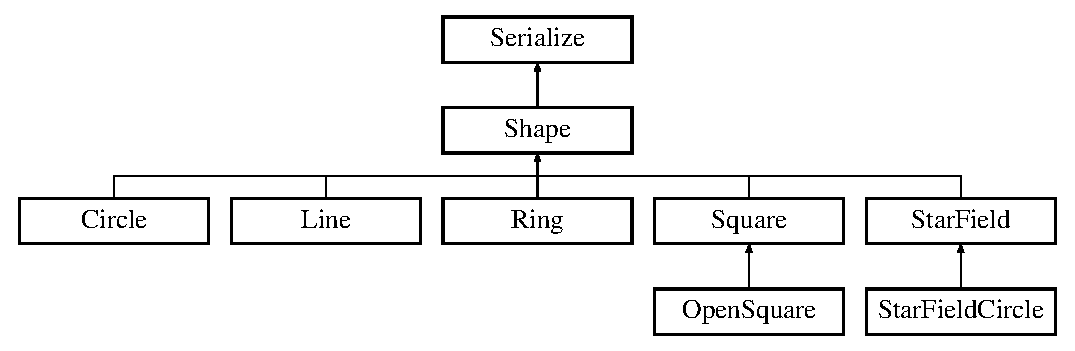
\includegraphics[height=4.000000cm]{classShape}
\end{center}
\end{figure}
\subsection*{Public Member Functions}
\begin{DoxyCompactItemize}
\item 
\hyperlink{classShape_a2c81e227edd2803a084c65c75e4ffd5b}{Shape} (void)
\item 
void \hyperlink{classShape_aa1d6e083d4bfe3793e53f30d092e6849}{delete\-Buffers} ()
\item 
virtual \hyperlink{classShape_a935afc9e576015f967d90de56977167d}{$\sim$\-Shape} ()
\item 
virtual void \hyperlink{classShape_afd5e29777ce90db927874c3a788fa7c1}{make\-V\-A\-O} (float $\ast$vertices, bool del, int display)
\item 
void \hyperlink{classShape_a7523425d407dd5087d8a036579560861}{make\-Shader} (int index, G\-Lenum type, std\-::string source)
\item 
std\-::string \hyperlink{classShape_a2ba56820a00ef275ce4e961fb633de5f}{file\-To\-String} (const char $\ast$fname)
\item 
void \hyperlink{classShape_a420de7854d2172951554999af84eb251}{make\-Shaders\-Named} (int index, const char $\ast$vertex\-Name, const char $\ast$fragment\-Name)
\item 
virtual void \hyperlink{classShape_a5503cd8cdc38875bcbe2e886f1609d7b}{make\-Shaders} (int index)
\item 
virtual void \hyperlink{classShape_a33be64d8e24518084b1c8f974f808387}{fill} (float $\ast$v)
\item 
virtual void \hyperlink{classShape_a5de43e4fb0921bac5f8a4a95e771e354}{configure} (int display)
\item 
void \hyperlink{classShape_a7d1f29c73622a3f32301ea59bfd89d32}{setup\-Draw\-Matrices} (int display, float)
\item 
virtual void \hyperlink{classShape_a892243993a2207807ab5069ce90bbef4}{draw} (int display, float ar)
\item 
virtual void \hyperlink{classShape_ac39d8d75d7498e3cd5395b8485fbf39f}{move} (long double)
\item 
unsigned char \hyperlink{classShape_ab001ba78956680cff154e302826f909d}{float\-To\-U8} (float in)
\begin{DoxyCompactList}\small\item\em serialization. \end{DoxyCompactList}\item 
virtual void \hyperlink{classShape_afc0a792fc9c31a0ae947f721c146f68b}{clear} ()
\item 
virtual bool \hyperlink{classShape_a9dea3f39fe203b2f4288dc7cda6295a7}{store} ()
\item 
virtual int \hyperlink{classShape_a92f5bc7b0179d1c47c2ae916727bf73d}{nstored} ()
\item 
virtual string \hyperlink{classShape_aaf3b0b140fcaf0bb11c28493ef745bfd}{store\-Name} (int indx)
\item 
virtual int \hyperlink{classShape_acf135c0569e45aa0fab16f748bee639e}{get\-Store\-Class} (int indx)
\item 
virtual void \hyperlink{classShape_afc3fbc26459718484ae4efe885f0fe37}{get\-Store\-Dims} (int indx, size\-\_\-t $\ast$dims)
\item 
virtual void $\ast$ \hyperlink{classShape_ae89da51d3c54b7b7139b8223103633e3}{get\-Store} (int indx, int i)
\item 
virtual int \hyperlink{classShape_a53bac379f3ad1537e56625015afd5c95}{num\-Stores} ()
\item 
virtual double $\ast$ \hyperlink{classShape_ae212539c5d1468805c155f4aed8367ea}{mmap\-Read} (double $\ast$d)
\end{DoxyCompactItemize}
\subsection*{Public Attributes}
\begin{DoxyCompactItemize}
\item 
bool \hyperlink{classShape_ac96ad62fd8b979f9a1e92b211922bb25}{m\-\_\-need\-Config} \mbox{[}2\mbox{]}
\item 
int \hyperlink{classShape_a14a1994dd7d7fc412b18d3ad2563556d}{m\-\_\-n}
\item 
unsigned int \hyperlink{classShape_a9a515d946d14526fe6d3cc566c4acf77}{m\-\_\-vao} \mbox{[}2\mbox{]}
\item 
unsigned int \hyperlink{classShape_af252a08a695affa2637645dcd4cdf4e9}{m\-\_\-vbo} \mbox{[}2\mbox{]}
\item 
unsigned int \hyperlink{classShape_a3cf20a9158443fa941b4e85a7b817816}{m\-\_\-drawmode}
\item 
double \hyperlink{classShape_aa8c2dca5ffd2e7f66cc4713e57ab029c}{m\-\_\-time}
\item 
char \hyperlink{classShape_a35589131828091da1fe3717f48e9c664}{m\-\_\-draw}
\item 
G\-Luint \hyperlink{classShape_a3689b5d3e0ab51e8e739699193ce9290}{m\-\_\-program} \mbox{[}2\mbox{]}
\item 
array$<$ float, 4 $>$ \hyperlink{classShape_a41389fbe5746a93b075acc98e485582c}{m\-\_\-color}
\item 
array$<$ float, 2 $>$ \hyperlink{classShape_a9af8ff3b5a90a8e42ea931969ec9428e}{m\-\_\-scale}
\item 
array$<$ float, 2 $>$ \hyperlink{classShape_ad2a5e6ad0362873a88ffcc69e5cb9b12}{m\-\_\-trans}
\item 
float \hyperlink{classShape_a43a38e552b2f2fc423dde3dd81dab0ce}{m\-\_\-rot}
\item 
vector$<$ double $>$ \hyperlink{classShape_af13b493550d418a20604baf5e1c8a0bd}{v\-\_\-time}
\item 
vector$<$ char $>$ \hyperlink{classShape_a6f426725f07e290ee150aab7be5b2587}{v\-\_\-draw}
\item 
vector$<$ array$<$ unsigned char, 4 $>$ $>$ \hyperlink{classShape_af3088673fcd7c8b642df4ecb157e53ff}{v\-\_\-color}
\item 
vector$<$ array$<$ float, 2 $>$ $>$ \hyperlink{classShape_ae2549de1dc4697ef18d2fa01d3e241b9}{v\-\_\-scale}
\item 
vector$<$ array$<$ float, 2 $>$ $>$ \hyperlink{classShape_a5fb4760689b0acae7a6088da0cba7d7b}{v\-\_\-trans}
\item 
vector$<$ float $>$ \hyperlink{classShape_a24f60964f7e4dc1b876a232f94948296}{v\-\_\-rot}
\end{DoxyCompactItemize}


\subsection{Constructor \& Destructor Documentation}
\hypertarget{classShape_a2c81e227edd2803a084c65c75e4ffd5b}{\index{Shape@{Shape}!Shape@{Shape}}
\index{Shape@{Shape}!Shape@{Shape}}
\subsubsection[{Shape}]{\setlength{\rightskip}{0pt plus 5cm}Shape\-::\-Shape (
\begin{DoxyParamCaption}
\item[{void}]{}
\end{DoxyParamCaption}
)}}\label{classShape_a2c81e227edd2803a084c65c75e4ffd5b}
\hypertarget{classShape_a935afc9e576015f967d90de56977167d}{\index{Shape@{Shape}!$\sim$\-Shape@{$\sim$\-Shape}}
\index{$\sim$\-Shape@{$\sim$\-Shape}!Shape@{Shape}}
\subsubsection[{$\sim$\-Shape}]{\setlength{\rightskip}{0pt plus 5cm}Shape\-::$\sim$\-Shape (
\begin{DoxyParamCaption}
{}
\end{DoxyParamCaption}
)\hspace{0.3cm}{\ttfamily [virtual]}}}\label{classShape_a935afc9e576015f967d90de56977167d}


\subsection{Member Function Documentation}
\hypertarget{classShape_afc0a792fc9c31a0ae947f721c146f68b}{\index{Shape@{Shape}!clear@{clear}}
\index{clear@{clear}!Shape@{Shape}}
\subsubsection[{clear}]{\setlength{\rightskip}{0pt plus 5cm}void Shape\-::clear (
\begin{DoxyParamCaption}
{}
\end{DoxyParamCaption}
)\hspace{0.3cm}{\ttfamily [virtual]}}}\label{classShape_afc0a792fc9c31a0ae947f721c146f68b}


Reimplemented from \hyperlink{classSerialize_a11cbf006415c08d1891ab42e39a2aa1a}{Serialize}.



Reimplemented in \hyperlink{classStarField_a1a97b6133ae0177f6eb8028470c28765}{Star\-Field}.

\hypertarget{classShape_a5de43e4fb0921bac5f8a4a95e771e354}{\index{Shape@{Shape}!configure@{configure}}
\index{configure@{configure}!Shape@{Shape}}
\subsubsection[{configure}]{\setlength{\rightskip}{0pt plus 5cm}void Shape\-::configure (
\begin{DoxyParamCaption}
\item[{int}]{display}
\end{DoxyParamCaption}
)\hspace{0.3cm}{\ttfamily [virtual]}}}\label{classShape_a5de43e4fb0921bac5f8a4a95e771e354}


Reimplemented in \hyperlink{classStarField_a0d5f438a2628b90e0d7ccc5a8683225b}{Star\-Field}.

\hypertarget{classShape_aa1d6e083d4bfe3793e53f30d092e6849}{\index{Shape@{Shape}!delete\-Buffers@{delete\-Buffers}}
\index{delete\-Buffers@{delete\-Buffers}!Shape@{Shape}}
\subsubsection[{delete\-Buffers}]{\setlength{\rightskip}{0pt plus 5cm}void Shape\-::delete\-Buffers (
\begin{DoxyParamCaption}
{}
\end{DoxyParamCaption}
)}}\label{classShape_aa1d6e083d4bfe3793e53f30d092e6849}
\hypertarget{classShape_a892243993a2207807ab5069ce90bbef4}{\index{Shape@{Shape}!draw@{draw}}
\index{draw@{draw}!Shape@{Shape}}
\subsubsection[{draw}]{\setlength{\rightskip}{0pt plus 5cm}void Shape\-::draw (
\begin{DoxyParamCaption}
\item[{int}]{display, }
\item[{float}]{ar}
\end{DoxyParamCaption}
)\hspace{0.3cm}{\ttfamily [virtual]}}}\label{classShape_a892243993a2207807ab5069ce90bbef4}


Reimplemented from \hyperlink{classSerialize_a0cf1d14e41052c6eabe53c90a37c227b}{Serialize}.



Reimplemented in \hyperlink{classStarField_aeaf743e6d1d4a8a6918152c40bd618c0}{Star\-Field}.

\hypertarget{classShape_a2ba56820a00ef275ce4e961fb633de5f}{\index{Shape@{Shape}!file\-To\-String@{file\-To\-String}}
\index{file\-To\-String@{file\-To\-String}!Shape@{Shape}}
\subsubsection[{file\-To\-String}]{\setlength{\rightskip}{0pt plus 5cm}std\-::string Shape\-::file\-To\-String (
\begin{DoxyParamCaption}
\item[{const char $\ast$}]{fname}
\end{DoxyParamCaption}
)}}\label{classShape_a2ba56820a00ef275ce4e961fb633de5f}
\hypertarget{classShape_a33be64d8e24518084b1c8f974f808387}{\index{Shape@{Shape}!fill@{fill}}
\index{fill@{fill}!Shape@{Shape}}
\subsubsection[{fill}]{\setlength{\rightskip}{0pt plus 5cm}void Shape\-::fill (
\begin{DoxyParamCaption}
\item[{float $\ast$}]{v}
\end{DoxyParamCaption}
)\hspace{0.3cm}{\ttfamily [virtual]}}}\label{classShape_a33be64d8e24518084b1c8f974f808387}


Reimplemented in \hyperlink{classRing_ad5dd2b058f6690108fe62da9d6e88d53}{Ring}, \hyperlink{classLine_a3f357683e8a9700cfc4d6f65f7f9493f}{Line}, \hyperlink{classSquare_aedaf26740b0f71c086886d5519cf44a6}{Square}, \hyperlink{classCircle_a59dab91c7a95f18e8b888a874c17826f}{Circle}, and \hyperlink{classOpenSquare_aa75c880448b327596b0b5fbde69e561c}{Open\-Square}.

\hypertarget{classShape_ab001ba78956680cff154e302826f909d}{\index{Shape@{Shape}!float\-To\-U8@{float\-To\-U8}}
\index{float\-To\-U8@{float\-To\-U8}!Shape@{Shape}}
\subsubsection[{float\-To\-U8}]{\setlength{\rightskip}{0pt plus 5cm}unsigned char Shape\-::float\-To\-U8 (
\begin{DoxyParamCaption}
\item[{float}]{in}
\end{DoxyParamCaption}
)}}\label{classShape_ab001ba78956680cff154e302826f909d}


serialization. 

\hypertarget{classShape_ae89da51d3c54b7b7139b8223103633e3}{\index{Shape@{Shape}!get\-Store@{get\-Store}}
\index{get\-Store@{get\-Store}!Shape@{Shape}}
\subsubsection[{get\-Store}]{\setlength{\rightskip}{0pt plus 5cm}void $\ast$ Shape\-::get\-Store (
\begin{DoxyParamCaption}
\item[{int}]{indx, }
\item[{int}]{i}
\end{DoxyParamCaption}
)\hspace{0.3cm}{\ttfamily [virtual]}}}\label{classShape_ae89da51d3c54b7b7139b8223103633e3}


Reimplemented from \hyperlink{classSerialize_a6e589d263cfdc0eb72e41687c58831f2}{Serialize}.



Reimplemented in \hyperlink{classStarField_a3d33db9d5e4c05a11cbe0c11a3bae5ba}{Star\-Field}.

\hypertarget{classShape_acf135c0569e45aa0fab16f748bee639e}{\index{Shape@{Shape}!get\-Store\-Class@{get\-Store\-Class}}
\index{get\-Store\-Class@{get\-Store\-Class}!Shape@{Shape}}
\subsubsection[{get\-Store\-Class}]{\setlength{\rightskip}{0pt plus 5cm}int Shape\-::get\-Store\-Class (
\begin{DoxyParamCaption}
\item[{int}]{indx}
\end{DoxyParamCaption}
)\hspace{0.3cm}{\ttfamily [virtual]}}}\label{classShape_acf135c0569e45aa0fab16f748bee639e}


Reimplemented from \hyperlink{classSerialize_a69954cc86d03b75b6b27511aec4aba43}{Serialize}.



Reimplemented in \hyperlink{classStarField_a42fa7234a0bb1e7b2e1d734fb9ed2dae}{Star\-Field}.

\hypertarget{classShape_afc3fbc26459718484ae4efe885f0fe37}{\index{Shape@{Shape}!get\-Store\-Dims@{get\-Store\-Dims}}
\index{get\-Store\-Dims@{get\-Store\-Dims}!Shape@{Shape}}
\subsubsection[{get\-Store\-Dims}]{\setlength{\rightskip}{0pt plus 5cm}void Shape\-::get\-Store\-Dims (
\begin{DoxyParamCaption}
\item[{int}]{indx, }
\item[{size\-\_\-t $\ast$}]{dims}
\end{DoxyParamCaption}
)\hspace{0.3cm}{\ttfamily [virtual]}}}\label{classShape_afc3fbc26459718484ae4efe885f0fe37}


Reimplemented from \hyperlink{classSerialize_a52034c5c17bc5e7e6c728b4e6c620c05}{Serialize}.



Reimplemented in \hyperlink{classStarField_a1cf58acb059f13adcb4b989120f99db5}{Star\-Field}.

\hypertarget{classShape_a7523425d407dd5087d8a036579560861}{\index{Shape@{Shape}!make\-Shader@{make\-Shader}}
\index{make\-Shader@{make\-Shader}!Shape@{Shape}}
\subsubsection[{make\-Shader}]{\setlength{\rightskip}{0pt plus 5cm}void Shape\-::make\-Shader (
\begin{DoxyParamCaption}
\item[{int}]{index, }
\item[{G\-Lenum}]{type, }
\item[{std\-::string}]{source}
\end{DoxyParamCaption}
)}}\label{classShape_a7523425d407dd5087d8a036579560861}
\hypertarget{classShape_a5503cd8cdc38875bcbe2e886f1609d7b}{\index{Shape@{Shape}!make\-Shaders@{make\-Shaders}}
\index{make\-Shaders@{make\-Shaders}!Shape@{Shape}}
\subsubsection[{make\-Shaders}]{\setlength{\rightskip}{0pt plus 5cm}void Shape\-::make\-Shaders (
\begin{DoxyParamCaption}
\item[{int}]{index}
\end{DoxyParamCaption}
)\hspace{0.3cm}{\ttfamily [virtual]}}}\label{classShape_a5503cd8cdc38875bcbe2e886f1609d7b}


Reimplemented in \hyperlink{classStarField_a72ab192923ffe6939fceb2166e05c82d}{Star\-Field}.

\hypertarget{classShape_a420de7854d2172951554999af84eb251}{\index{Shape@{Shape}!make\-Shaders\-Named@{make\-Shaders\-Named}}
\index{make\-Shaders\-Named@{make\-Shaders\-Named}!Shape@{Shape}}
\subsubsection[{make\-Shaders\-Named}]{\setlength{\rightskip}{0pt plus 5cm}void Shape\-::make\-Shaders\-Named (
\begin{DoxyParamCaption}
\item[{int}]{index, }
\item[{const char $\ast$}]{vertex\-Name, }
\item[{const char $\ast$}]{fragment\-Name}
\end{DoxyParamCaption}
)}}\label{classShape_a420de7854d2172951554999af84eb251}
\hypertarget{classShape_afd5e29777ce90db927874c3a788fa7c1}{\index{Shape@{Shape}!make\-V\-A\-O@{make\-V\-A\-O}}
\index{make\-V\-A\-O@{make\-V\-A\-O}!Shape@{Shape}}
\subsubsection[{make\-V\-A\-O}]{\setlength{\rightskip}{0pt plus 5cm}void Shape\-::make\-V\-A\-O (
\begin{DoxyParamCaption}
\item[{float $\ast$}]{vertices, }
\item[{bool}]{del, }
\item[{int}]{display}
\end{DoxyParamCaption}
)\hspace{0.3cm}{\ttfamily [virtual]}}}\label{classShape_afd5e29777ce90db927874c3a788fa7c1}
\hypertarget{classShape_ae212539c5d1468805c155f4aed8367ea}{\index{Shape@{Shape}!mmap\-Read@{mmap\-Read}}
\index{mmap\-Read@{mmap\-Read}!Shape@{Shape}}
\subsubsection[{mmap\-Read}]{\setlength{\rightskip}{0pt plus 5cm}double $\ast$ Shape\-::mmap\-Read (
\begin{DoxyParamCaption}
\item[{double $\ast$}]{d}
\end{DoxyParamCaption}
)\hspace{0.3cm}{\ttfamily [virtual]}}}\label{classShape_ae212539c5d1468805c155f4aed8367ea}


Reimplemented from \hyperlink{classSerialize_a28b939242880e565a8906b30acd0f84c}{Serialize}.



Reimplemented in \hyperlink{classStarField_a6937d614690f774772920ae9faee9bab}{Star\-Field}.

\hypertarget{classShape_ac39d8d75d7498e3cd5395b8485fbf39f}{\index{Shape@{Shape}!move@{move}}
\index{move@{move}!Shape@{Shape}}
\subsubsection[{move}]{\setlength{\rightskip}{0pt plus 5cm}void Shape\-::move (
\begin{DoxyParamCaption}
\item[{long double}]{}
\end{DoxyParamCaption}
)\hspace{0.3cm}{\ttfamily [virtual]}}}\label{classShape_ac39d8d75d7498e3cd5395b8485fbf39f}


Reimplemented from \hyperlink{classSerialize_a06cf228664e659c8490c63ee36f34e28}{Serialize}.



Reimplemented in \hyperlink{classStarField_ac3e35d838577ed7610bdaf933ef5b99d}{Star\-Field}, and \hyperlink{classStarFieldCircle_af54e17032bb1ee195137b3585e7caea5}{Star\-Field\-Circle}.

\hypertarget{classShape_a92f5bc7b0179d1c47c2ae916727bf73d}{\index{Shape@{Shape}!nstored@{nstored}}
\index{nstored@{nstored}!Shape@{Shape}}
\subsubsection[{nstored}]{\setlength{\rightskip}{0pt plus 5cm}int Shape\-::nstored (
\begin{DoxyParamCaption}
{}
\end{DoxyParamCaption}
)\hspace{0.3cm}{\ttfamily [virtual]}}}\label{classShape_a92f5bc7b0179d1c47c2ae916727bf73d}


Reimplemented from \hyperlink{classSerialize_a590b7308112b07581c03ba826ace50b4}{Serialize}.

\hypertarget{classShape_a53bac379f3ad1537e56625015afd5c95}{\index{Shape@{Shape}!num\-Stores@{num\-Stores}}
\index{num\-Stores@{num\-Stores}!Shape@{Shape}}
\subsubsection[{num\-Stores}]{\setlength{\rightskip}{0pt plus 5cm}int Shape\-::num\-Stores (
\begin{DoxyParamCaption}
{}
\end{DoxyParamCaption}
)\hspace{0.3cm}{\ttfamily [virtual]}}}\label{classShape_a53bac379f3ad1537e56625015afd5c95}


Reimplemented from \hyperlink{classSerialize_a71bf2a906fd71477308a942d01490ab3}{Serialize}.



Reimplemented in \hyperlink{classStarField_a1289224a6763a69ac041eb32d685b657}{Star\-Field}.

\hypertarget{classShape_a7d1f29c73622a3f32301ea59bfd89d32}{\index{Shape@{Shape}!setup\-Draw\-Matrices@{setup\-Draw\-Matrices}}
\index{setup\-Draw\-Matrices@{setup\-Draw\-Matrices}!Shape@{Shape}}
\subsubsection[{setup\-Draw\-Matrices}]{\setlength{\rightskip}{0pt plus 5cm}void Shape\-::setup\-Draw\-Matrices (
\begin{DoxyParamCaption}
\item[{int}]{display, }
\item[{float}]{}
\end{DoxyParamCaption}
)}}\label{classShape_a7d1f29c73622a3f32301ea59bfd89d32}
\hypertarget{classShape_a9dea3f39fe203b2f4288dc7cda6295a7}{\index{Shape@{Shape}!store@{store}}
\index{store@{store}!Shape@{Shape}}
\subsubsection[{store}]{\setlength{\rightskip}{0pt plus 5cm}bool Shape\-::store (
\begin{DoxyParamCaption}
{}
\end{DoxyParamCaption}
)\hspace{0.3cm}{\ttfamily [virtual]}}}\label{classShape_a9dea3f39fe203b2f4288dc7cda6295a7}


Reimplemented from \hyperlink{classSerialize_a3cda20e84a530870a6115eaaf589f168}{Serialize}.



Reimplemented in \hyperlink{classStarField_aa8411004d05d05ac3e0f8d10bfa1949e}{Star\-Field}.

\hypertarget{classShape_aaf3b0b140fcaf0bb11c28493ef745bfd}{\index{Shape@{Shape}!store\-Name@{store\-Name}}
\index{store\-Name@{store\-Name}!Shape@{Shape}}
\subsubsection[{store\-Name}]{\setlength{\rightskip}{0pt plus 5cm}string Shape\-::store\-Name (
\begin{DoxyParamCaption}
\item[{int}]{indx}
\end{DoxyParamCaption}
)\hspace{0.3cm}{\ttfamily [virtual]}}}\label{classShape_aaf3b0b140fcaf0bb11c28493ef745bfd}


Reimplemented from \hyperlink{classSerialize_ac94a76de6c9376e33b4c195d50ff0568}{Serialize}.



Reimplemented in \hyperlink{classStarField_a047f987e052fc14fd8041658c153e0f1}{Star\-Field}.



\subsection{Member Data Documentation}
\hypertarget{classShape_a41389fbe5746a93b075acc98e485582c}{\index{Shape@{Shape}!m\-\_\-color@{m\-\_\-color}}
\index{m\-\_\-color@{m\-\_\-color}!Shape@{Shape}}
\subsubsection[{m\-\_\-color}]{\setlength{\rightskip}{0pt plus 5cm}array$<$float,4$>$ Shape\-::m\-\_\-color}}\label{classShape_a41389fbe5746a93b075acc98e485582c}
\hypertarget{classShape_a35589131828091da1fe3717f48e9c664}{\index{Shape@{Shape}!m\-\_\-draw@{m\-\_\-draw}}
\index{m\-\_\-draw@{m\-\_\-draw}!Shape@{Shape}}
\subsubsection[{m\-\_\-draw}]{\setlength{\rightskip}{0pt plus 5cm}char Shape\-::m\-\_\-draw}}\label{classShape_a35589131828091da1fe3717f48e9c664}
\hypertarget{classShape_a3cf20a9158443fa941b4e85a7b817816}{\index{Shape@{Shape}!m\-\_\-drawmode@{m\-\_\-drawmode}}
\index{m\-\_\-drawmode@{m\-\_\-drawmode}!Shape@{Shape}}
\subsubsection[{m\-\_\-drawmode}]{\setlength{\rightskip}{0pt plus 5cm}unsigned int Shape\-::m\-\_\-drawmode}}\label{classShape_a3cf20a9158443fa941b4e85a7b817816}
\hypertarget{classShape_a14a1994dd7d7fc412b18d3ad2563556d}{\index{Shape@{Shape}!m\-\_\-n@{m\-\_\-n}}
\index{m\-\_\-n@{m\-\_\-n}!Shape@{Shape}}
\subsubsection[{m\-\_\-n}]{\setlength{\rightskip}{0pt plus 5cm}int Shape\-::m\-\_\-n}}\label{classShape_a14a1994dd7d7fc412b18d3ad2563556d}
\hypertarget{classShape_ac96ad62fd8b979f9a1e92b211922bb25}{\index{Shape@{Shape}!m\-\_\-need\-Config@{m\-\_\-need\-Config}}
\index{m\-\_\-need\-Config@{m\-\_\-need\-Config}!Shape@{Shape}}
\subsubsection[{m\-\_\-need\-Config}]{\setlength{\rightskip}{0pt plus 5cm}bool Shape\-::m\-\_\-need\-Config\mbox{[}2\mbox{]}}}\label{classShape_ac96ad62fd8b979f9a1e92b211922bb25}
\hypertarget{classShape_a3689b5d3e0ab51e8e739699193ce9290}{\index{Shape@{Shape}!m\-\_\-program@{m\-\_\-program}}
\index{m\-\_\-program@{m\-\_\-program}!Shape@{Shape}}
\subsubsection[{m\-\_\-program}]{\setlength{\rightskip}{0pt plus 5cm}G\-Luint Shape\-::m\-\_\-program\mbox{[}2\mbox{]}}}\label{classShape_a3689b5d3e0ab51e8e739699193ce9290}
\hypertarget{classShape_a43a38e552b2f2fc423dde3dd81dab0ce}{\index{Shape@{Shape}!m\-\_\-rot@{m\-\_\-rot}}
\index{m\-\_\-rot@{m\-\_\-rot}!Shape@{Shape}}
\subsubsection[{m\-\_\-rot}]{\setlength{\rightskip}{0pt plus 5cm}float Shape\-::m\-\_\-rot}}\label{classShape_a43a38e552b2f2fc423dde3dd81dab0ce}
\hypertarget{classShape_a9af8ff3b5a90a8e42ea931969ec9428e}{\index{Shape@{Shape}!m\-\_\-scale@{m\-\_\-scale}}
\index{m\-\_\-scale@{m\-\_\-scale}!Shape@{Shape}}
\subsubsection[{m\-\_\-scale}]{\setlength{\rightskip}{0pt plus 5cm}array$<$float,2$>$ Shape\-::m\-\_\-scale}}\label{classShape_a9af8ff3b5a90a8e42ea931969ec9428e}
\hypertarget{classShape_aa8c2dca5ffd2e7f66cc4713e57ab029c}{\index{Shape@{Shape}!m\-\_\-time@{m\-\_\-time}}
\index{m\-\_\-time@{m\-\_\-time}!Shape@{Shape}}
\subsubsection[{m\-\_\-time}]{\setlength{\rightskip}{0pt plus 5cm}double Shape\-::m\-\_\-time}}\label{classShape_aa8c2dca5ffd2e7f66cc4713e57ab029c}
\hypertarget{classShape_ad2a5e6ad0362873a88ffcc69e5cb9b12}{\index{Shape@{Shape}!m\-\_\-trans@{m\-\_\-trans}}
\index{m\-\_\-trans@{m\-\_\-trans}!Shape@{Shape}}
\subsubsection[{m\-\_\-trans}]{\setlength{\rightskip}{0pt plus 5cm}array$<$float,2$>$ Shape\-::m\-\_\-trans}}\label{classShape_ad2a5e6ad0362873a88ffcc69e5cb9b12}
\hypertarget{classShape_a9a515d946d14526fe6d3cc566c4acf77}{\index{Shape@{Shape}!m\-\_\-vao@{m\-\_\-vao}}
\index{m\-\_\-vao@{m\-\_\-vao}!Shape@{Shape}}
\subsubsection[{m\-\_\-vao}]{\setlength{\rightskip}{0pt plus 5cm}unsigned int Shape\-::m\-\_\-vao\mbox{[}2\mbox{]}}}\label{classShape_a9a515d946d14526fe6d3cc566c4acf77}
\hypertarget{classShape_af252a08a695affa2637645dcd4cdf4e9}{\index{Shape@{Shape}!m\-\_\-vbo@{m\-\_\-vbo}}
\index{m\-\_\-vbo@{m\-\_\-vbo}!Shape@{Shape}}
\subsubsection[{m\-\_\-vbo}]{\setlength{\rightskip}{0pt plus 5cm}unsigned int Shape\-::m\-\_\-vbo\mbox{[}2\mbox{]}}}\label{classShape_af252a08a695affa2637645dcd4cdf4e9}
\hypertarget{classShape_af3088673fcd7c8b642df4ecb157e53ff}{\index{Shape@{Shape}!v\-\_\-color@{v\-\_\-color}}
\index{v\-\_\-color@{v\-\_\-color}!Shape@{Shape}}
\subsubsection[{v\-\_\-color}]{\setlength{\rightskip}{0pt plus 5cm}vector$<$array$<$unsigned char,4$>$ $>$ Shape\-::v\-\_\-color}}\label{classShape_af3088673fcd7c8b642df4ecb157e53ff}
\hypertarget{classShape_a6f426725f07e290ee150aab7be5b2587}{\index{Shape@{Shape}!v\-\_\-draw@{v\-\_\-draw}}
\index{v\-\_\-draw@{v\-\_\-draw}!Shape@{Shape}}
\subsubsection[{v\-\_\-draw}]{\setlength{\rightskip}{0pt plus 5cm}vector$<$char$>$ Shape\-::v\-\_\-draw}}\label{classShape_a6f426725f07e290ee150aab7be5b2587}
\hypertarget{classShape_a24f60964f7e4dc1b876a232f94948296}{\index{Shape@{Shape}!v\-\_\-rot@{v\-\_\-rot}}
\index{v\-\_\-rot@{v\-\_\-rot}!Shape@{Shape}}
\subsubsection[{v\-\_\-rot}]{\setlength{\rightskip}{0pt plus 5cm}vector$<$float$>$ Shape\-::v\-\_\-rot}}\label{classShape_a24f60964f7e4dc1b876a232f94948296}
\hypertarget{classShape_ae2549de1dc4697ef18d2fa01d3e241b9}{\index{Shape@{Shape}!v\-\_\-scale@{v\-\_\-scale}}
\index{v\-\_\-scale@{v\-\_\-scale}!Shape@{Shape}}
\subsubsection[{v\-\_\-scale}]{\setlength{\rightskip}{0pt plus 5cm}vector$<$array$<$float,2$>$ $>$ Shape\-::v\-\_\-scale}}\label{classShape_ae2549de1dc4697ef18d2fa01d3e241b9}
\hypertarget{classShape_af13b493550d418a20604baf5e1c8a0bd}{\index{Shape@{Shape}!v\-\_\-time@{v\-\_\-time}}
\index{v\-\_\-time@{v\-\_\-time}!Shape@{Shape}}
\subsubsection[{v\-\_\-time}]{\setlength{\rightskip}{0pt plus 5cm}vector$<$double$>$ Shape\-::v\-\_\-time}}\label{classShape_af13b493550d418a20604baf5e1c8a0bd}
\hypertarget{classShape_a5fb4760689b0acae7a6088da0cba7d7b}{\index{Shape@{Shape}!v\-\_\-trans@{v\-\_\-trans}}
\index{v\-\_\-trans@{v\-\_\-trans}!Shape@{Shape}}
\subsubsection[{v\-\_\-trans}]{\setlength{\rightskip}{0pt plus 5cm}vector$<$array$<$float,2$>$ $>$ Shape\-::v\-\_\-trans}}\label{classShape_a5fb4760689b0acae7a6088da0cba7d7b}


The documentation for this class was generated from the following files\-:\begin{DoxyCompactItemize}
\item 
/home/ruijan/sw/bmi5/bmi5/include/\-Shape/\hyperlink{shape_8h}{shape.\-h}\item 
/home/ruijan/sw/bmi5/bmi5/src/\-Shape/\hyperlink{shape_8cpp}{shape.\-cpp}\end{DoxyCompactItemize}

\hypertarget{classSquare}{\section{Square Class Reference}
\label{classSquare}\index{Square@{Square}}
}


{\ttfamily \#include $<$square.\-h$>$}

Inheritance diagram for Square\-:\begin{figure}[H]
\begin{center}
\leavevmode
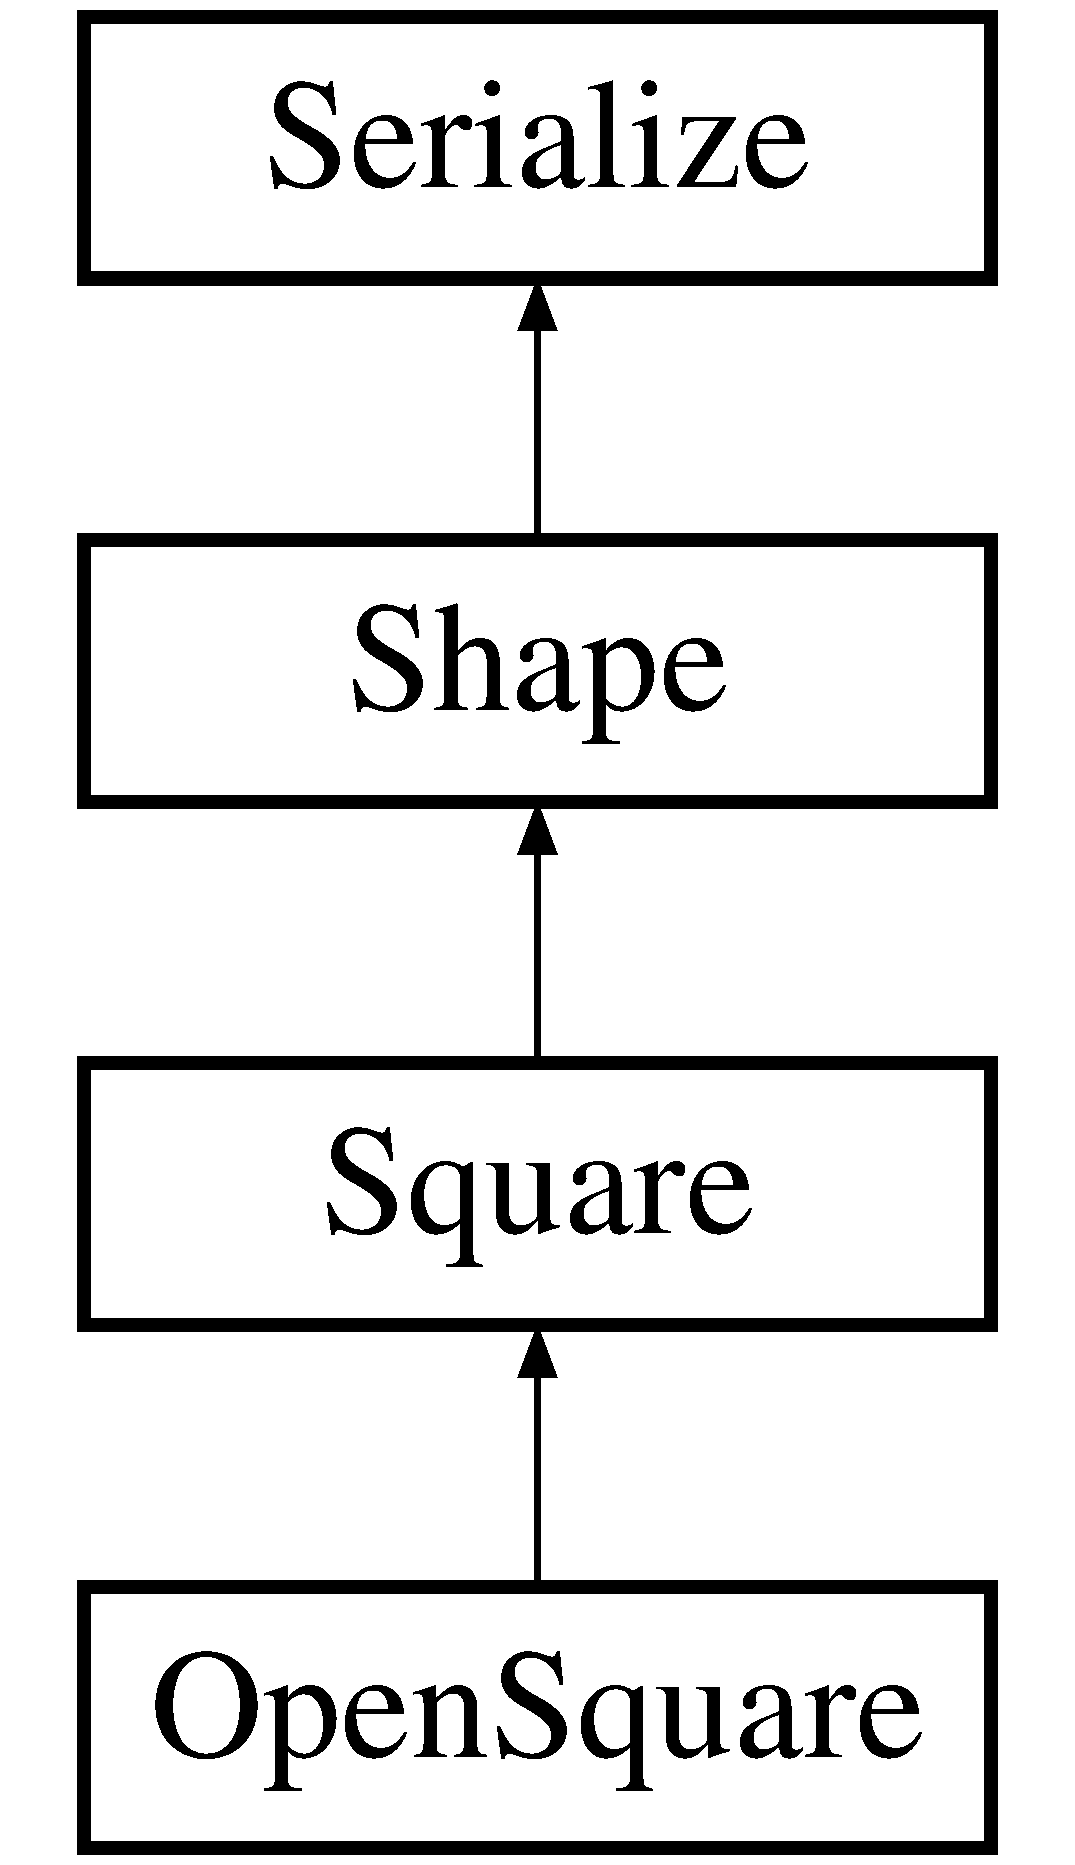
\includegraphics[height=4.000000cm]{classSquare}
\end{center}
\end{figure}
\subsection*{Public Member Functions}
\begin{DoxyCompactItemize}
\item 
\hyperlink{classSquare_ae08fc41594d222353ce211889f1b9116}{Square} (float width)
\item 
\hyperlink{classSquare_a90af7ce1060cff7b717ceddb333846b8}{$\sim$\-Square} ()
\item 
virtual void \hyperlink{classSquare_aedaf26740b0f71c086886d5519cf44a6}{fill} (float $\ast$v)
\end{DoxyCompactItemize}
\subsection*{Public Attributes}
\begin{DoxyCompactItemize}
\item 
float \hyperlink{classSquare_ab590a983d9ff84dd6d337e40697ae0d6}{m\-\_\-w}
\item 
float \hyperlink{classSquare_ad4f52dd3d5d29f77db924c3ce447de47}{m\-\_\-sign} \mbox{[}10\mbox{]} = \{-\/1,-\/1,-\/1,1,1,1,1,-\/1,-\/1,-\/1\}
\end{DoxyCompactItemize}


\subsection{Constructor \& Destructor Documentation}
\hypertarget{classSquare_ae08fc41594d222353ce211889f1b9116}{\index{Square@{Square}!Square@{Square}}
\index{Square@{Square}!Square@{Square}}
\subsubsection[{Square}]{\setlength{\rightskip}{0pt plus 5cm}Square\-::\-Square (
\begin{DoxyParamCaption}
\item[{float}]{width}
\end{DoxyParamCaption}
)}}\label{classSquare_ae08fc41594d222353ce211889f1b9116}
\hypertarget{classSquare_a90af7ce1060cff7b717ceddb333846b8}{\index{Square@{Square}!$\sim$\-Square@{$\sim$\-Square}}
\index{$\sim$\-Square@{$\sim$\-Square}!Square@{Square}}
\subsubsection[{$\sim$\-Square}]{\setlength{\rightskip}{0pt plus 5cm}Square\-::$\sim$\-Square (
\begin{DoxyParamCaption}
{}
\end{DoxyParamCaption}
)}}\label{classSquare_a90af7ce1060cff7b717ceddb333846b8}


\subsection{Member Function Documentation}
\hypertarget{classSquare_aedaf26740b0f71c086886d5519cf44a6}{\index{Square@{Square}!fill@{fill}}
\index{fill@{fill}!Square@{Square}}
\subsubsection[{fill}]{\setlength{\rightskip}{0pt plus 5cm}void Square\-::fill (
\begin{DoxyParamCaption}
\item[{float $\ast$}]{v}
\end{DoxyParamCaption}
)\hspace{0.3cm}{\ttfamily [virtual]}}}\label{classSquare_aedaf26740b0f71c086886d5519cf44a6}


Reimplemented from \hyperlink{classShape_a33be64d8e24518084b1c8f974f808387}{Shape}.



Reimplemented in \hyperlink{classOpenSquare_aa75c880448b327596b0b5fbde69e561c}{Open\-Square}.



\subsection{Member Data Documentation}
\hypertarget{classSquare_ad4f52dd3d5d29f77db924c3ce447de47}{\index{Square@{Square}!m\-\_\-sign@{m\-\_\-sign}}
\index{m\-\_\-sign@{m\-\_\-sign}!Square@{Square}}
\subsubsection[{m\-\_\-sign}]{\setlength{\rightskip}{0pt plus 5cm}float Square\-::m\-\_\-sign\mbox{[}10\mbox{]} = \{-\/1,-\/1,-\/1,1,1,1,1,-\/1,-\/1,-\/1\}}}\label{classSquare_ad4f52dd3d5d29f77db924c3ce447de47}
\hypertarget{classSquare_ab590a983d9ff84dd6d337e40697ae0d6}{\index{Square@{Square}!m\-\_\-w@{m\-\_\-w}}
\index{m\-\_\-w@{m\-\_\-w}!Square@{Square}}
\subsubsection[{m\-\_\-w}]{\setlength{\rightskip}{0pt plus 5cm}float Square\-::m\-\_\-w}}\label{classSquare_ab590a983d9ff84dd6d337e40697ae0d6}


The documentation for this class was generated from the following files\-:\begin{DoxyCompactItemize}
\item 
/home/ruijan/sw/bmi5/bmi5/include/\-Shape/\hyperlink{square_8h}{square.\-h}\item 
/home/ruijan/sw/bmi5/bmi5/src/\-Shape/\hyperlink{square_8cpp}{square.\-cpp}\end{DoxyCompactItemize}

\hypertarget{classStarField}{\section{Star\-Field Class Reference}
\label{classStarField}\index{Star\-Field@{Star\-Field}}
}


{\ttfamily \#include $<$star\-Field.\-h$>$}

Inheritance diagram for Star\-Field\-:\begin{figure}[H]
\begin{center}
\leavevmode
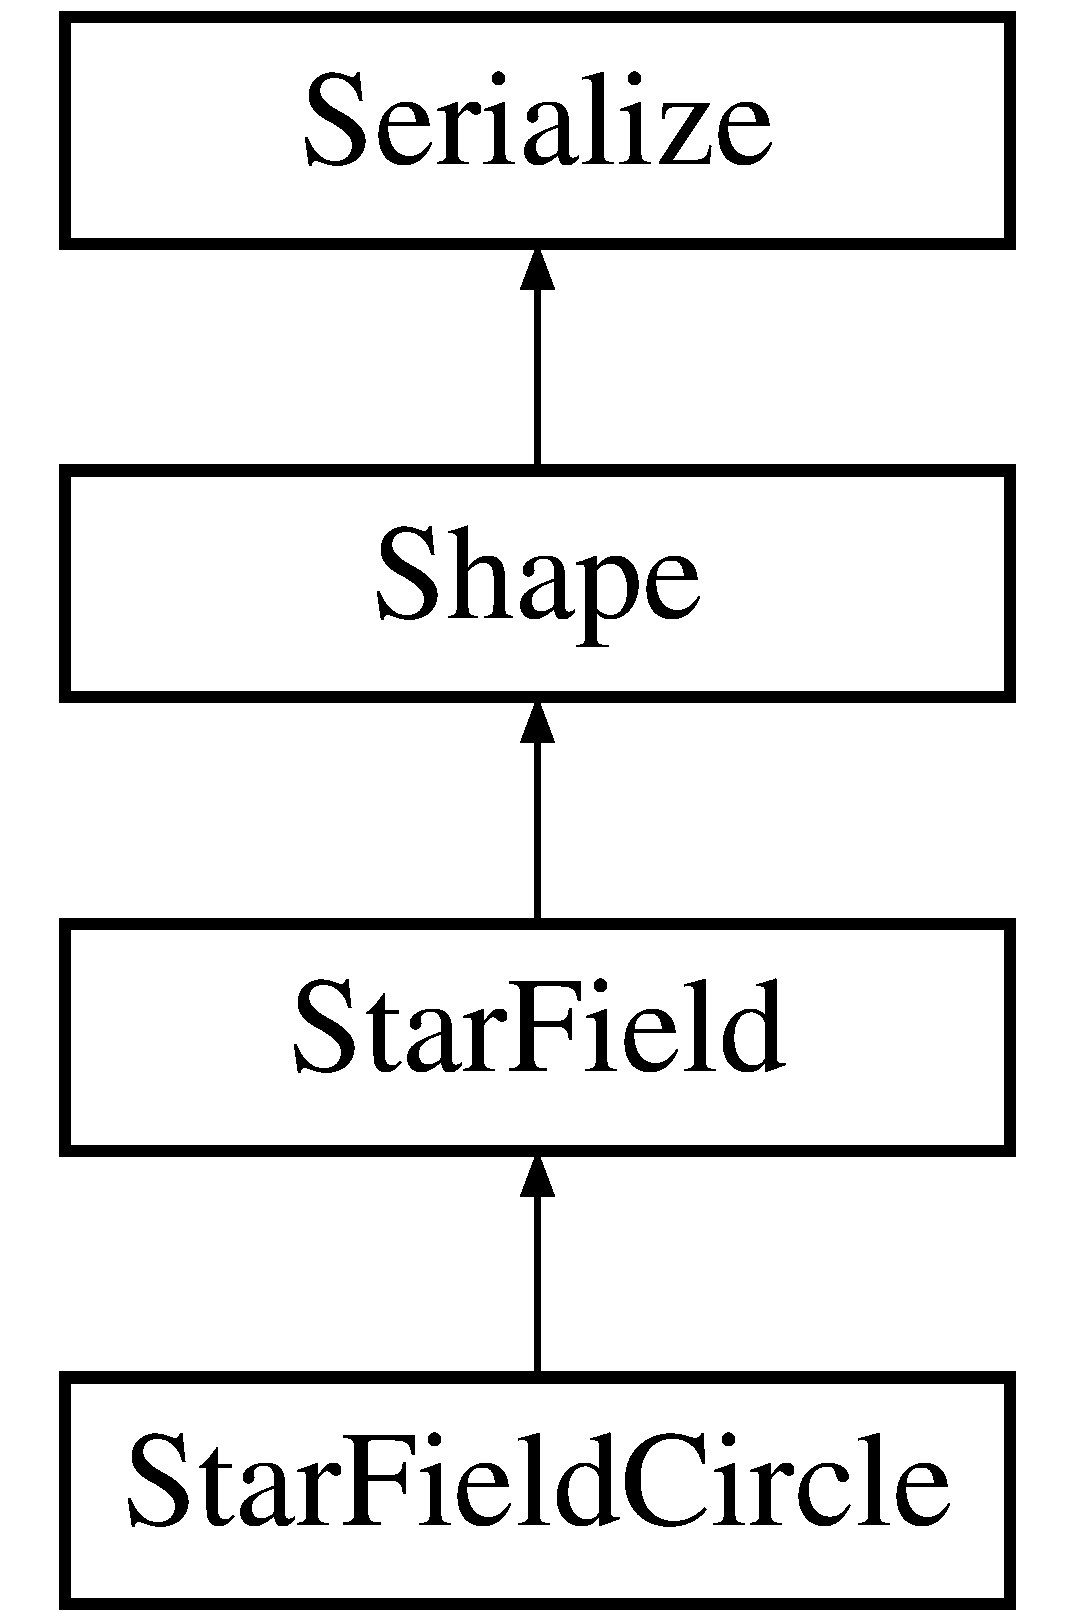
\includegraphics[height=4.000000cm]{classStarField}
\end{center}
\end{figure}
\subsection*{Public Member Functions}
\begin{DoxyCompactItemize}
\item 
\hyperlink{classStarField_ab2bd0288efac030b0f4dabe9f07f5e4e}{Star\-Field} ()
\item 
\hyperlink{classStarField_a01b259387dc4a83272901110c30d4cb2}{$\sim$\-Star\-Field} ()
\item 
virtual void \hyperlink{classStarField_afb99580b3907e4c271040f332262fb1c}{make\-V\-A\-O} (\hyperlink{structstarStruct}{star\-Struct} $\ast$vertices, bool del, int display)
\item 
float \hyperlink{classStarField_a69aeb2f24c09fbb2cccb79e5135d4bc8}{uniform} ()
\item 
float \hyperlink{classStarField_ad2e8a935f3c810330bfb61d7404b986e}{norm} (float a, float b)
\item 
virtual void \hyperlink{classStarField_ae6b25b3827440dedf5836070205d4c6d}{make\-Stars} (int nstars)
\item 
virtual void \hyperlink{classStarField_a72ab192923ffe6939fceb2166e05c82d}{make\-Shaders} (int index)
\item 
virtual void \hyperlink{classStarField_a0d5f438a2628b90e0d7ccc5a8683225b}{configure} (int display)
\item 
virtual void \hyperlink{classStarField_ac3e35d838577ed7610bdaf933ef5b99d}{move} (long double time)
\item 
virtual void \hyperlink{classStarField_aeaf743e6d1d4a8a6918152c40bd618c0}{draw} (int display, float ar)
\item 
void \hyperlink{classStarField_a01b9571dbc4f28f0a75b12790e11cd8e}{set\-Vel} (double x, double y)
\item 
void \hyperlink{classStarField_adc2425bc84abe280cbe53229f7b167b2}{set\-Coherence} (double c)
\item 
void \hyperlink{classStarField_a641c0759d85fbb2f8adbbf6e7a2e636b}{set\-Lifetime} (double x)
\item 
void \hyperlink{classStarField_acf8cd47946ce81cd7256d6f162c4b67e}{set\-Star\-Size} (double ss)
\item 
virtual void \hyperlink{classStarField_a1a97b6133ae0177f6eb8028470c28765}{clear} ()
\item 
virtual bool \hyperlink{classStarField_aa8411004d05d05ac3e0f8d10bfa1949e}{store} ()
\item 
virtual string \hyperlink{classStarField_a047f987e052fc14fd8041658c153e0f1}{store\-Name} (int indx)
\item 
virtual int \hyperlink{classStarField_a42fa7234a0bb1e7b2e1d734fb9ed2dae}{get\-Store\-Class} (int indx)
\item 
virtual void \hyperlink{classStarField_a1cf58acb059f13adcb4b989120f99db5}{get\-Store\-Dims} (int indx, size\-\_\-t $\ast$dims)
\item 
virtual void $\ast$ \hyperlink{classStarField_a3d33db9d5e4c05a11cbe0c11a3bae5ba}{get\-Store} (int indx, int i)
\item 
virtual int \hyperlink{classStarField_a1289224a6763a69ac041eb32d685b657}{num\-Stores} ()
\item 
virtual double $\ast$ \hyperlink{classStarField_a6937d614690f774772920ae9faee9bab}{mmap\-Read} (double $\ast$d)
\end{DoxyCompactItemize}
\subsection*{Public Attributes}
\begin{DoxyCompactItemize}
\item 
array$<$ float, 2 $>$ \hyperlink{classStarField_a21ba5382655395de9cce3328cf4be730}{m\-\_\-vel}
\item 
double $\ast$ \hyperlink{classStarField_a922034700e887585b42b80df399ddede}{m\-\_\-phase}
\item 
\hyperlink{structstarStruct}{star\-Struct} $\ast$ \hyperlink{classStarField_af6c1cf901231fd963efaa1c8ed1eca5d}{m\-\_\-v}
\item 
float $\ast$ \hyperlink{classStarField_a483be12bd49068c4f46a14dfc733a2ca}{m\-\_\-pvel}
\item 
float \hyperlink{classStarField_a65a4e5967dd2e328274d61cf8a5c50ba}{m\-\_\-coherence}
\item 
float \hyperlink{classStarField_adf36490fe3843a374b437b2fc1f482d6}{m\-\_\-starsize}
\item 
float \hyperlink{classStarField_a575970efe2365bb4dfa1b1b2eebafbd7}{m\-\_\-lifetime}
\item 
G\-Luint \hyperlink{classStarField_aa3e4c31177f3c5be4f11e629e4a1b5a6}{m\-\_\-colorbuffer}
\item 
long double \hyperlink{classStarField_a04bcafb900567a3b87f9c910614c8fa4}{m\-\_\-last\-Time}
\item 
long double \hyperlink{classStarField_a71f79afd2f64f68bae9edf978b579c5d}{m\-\_\-start\-Time}
\item 
vector$<$ array$<$ float, 2 $>$ $>$ \hyperlink{classStarField_a28482b3624fa5204a35faf1dbca6136c}{v\-\_\-vel}
\item 
vector$<$ float $>$ \hyperlink{classStarField_a9184ebba5f686d75ac8ee3c3da3b3f64}{v\-\_\-coherence}
\item 
vector$<$ float $>$ \hyperlink{classStarField_a3090733382397dd067da0f60d26085c0}{v\-\_\-lifetime}
\item 
vector$<$ float $>$ \hyperlink{classStarField_ac66cfbc7ac7d40cd1c7f0b7bf6b5dd1a}{v\-\_\-starsize}
\end{DoxyCompactItemize}


\subsection{Constructor \& Destructor Documentation}
\hypertarget{classStarField_ab2bd0288efac030b0f4dabe9f07f5e4e}{\index{Star\-Field@{Star\-Field}!Star\-Field@{Star\-Field}}
\index{Star\-Field@{Star\-Field}!StarField@{Star\-Field}}
\subsubsection[{Star\-Field}]{\setlength{\rightskip}{0pt plus 5cm}Star\-Field\-::\-Star\-Field (
\begin{DoxyParamCaption}
{}
\end{DoxyParamCaption}
)}}\label{classStarField_ab2bd0288efac030b0f4dabe9f07f5e4e}
\hypertarget{classStarField_a01b259387dc4a83272901110c30d4cb2}{\index{Star\-Field@{Star\-Field}!$\sim$\-Star\-Field@{$\sim$\-Star\-Field}}
\index{$\sim$\-Star\-Field@{$\sim$\-Star\-Field}!StarField@{Star\-Field}}
\subsubsection[{$\sim$\-Star\-Field}]{\setlength{\rightskip}{0pt plus 5cm}Star\-Field\-::$\sim$\-Star\-Field (
\begin{DoxyParamCaption}
{}
\end{DoxyParamCaption}
)}}\label{classStarField_a01b259387dc4a83272901110c30d4cb2}


\subsection{Member Function Documentation}
\hypertarget{classStarField_a1a97b6133ae0177f6eb8028470c28765}{\index{Star\-Field@{Star\-Field}!clear@{clear}}
\index{clear@{clear}!StarField@{Star\-Field}}
\subsubsection[{clear}]{\setlength{\rightskip}{0pt plus 5cm}void Star\-Field\-::clear (
\begin{DoxyParamCaption}
{}
\end{DoxyParamCaption}
)\hspace{0.3cm}{\ttfamily [virtual]}}}\label{classStarField_a1a97b6133ae0177f6eb8028470c28765}


Reimplemented from \hyperlink{classShape_afc0a792fc9c31a0ae947f721c146f68b}{Shape}.

\hypertarget{classStarField_a0d5f438a2628b90e0d7ccc5a8683225b}{\index{Star\-Field@{Star\-Field}!configure@{configure}}
\index{configure@{configure}!StarField@{Star\-Field}}
\subsubsection[{configure}]{\setlength{\rightskip}{0pt plus 5cm}void Star\-Field\-::configure (
\begin{DoxyParamCaption}
\item[{int}]{display}
\end{DoxyParamCaption}
)\hspace{0.3cm}{\ttfamily [virtual]}}}\label{classStarField_a0d5f438a2628b90e0d7ccc5a8683225b}


Reimplemented from \hyperlink{classShape_a5de43e4fb0921bac5f8a4a95e771e354}{Shape}.

\hypertarget{classStarField_aeaf743e6d1d4a8a6918152c40bd618c0}{\index{Star\-Field@{Star\-Field}!draw@{draw}}
\index{draw@{draw}!StarField@{Star\-Field}}
\subsubsection[{draw}]{\setlength{\rightskip}{0pt plus 5cm}void Star\-Field\-::draw (
\begin{DoxyParamCaption}
\item[{int}]{display, }
\item[{float}]{ar}
\end{DoxyParamCaption}
)\hspace{0.3cm}{\ttfamily [virtual]}}}\label{classStarField_aeaf743e6d1d4a8a6918152c40bd618c0}


Reimplemented from \hyperlink{classShape_a892243993a2207807ab5069ce90bbef4}{Shape}.

\hypertarget{classStarField_a3d33db9d5e4c05a11cbe0c11a3bae5ba}{\index{Star\-Field@{Star\-Field}!get\-Store@{get\-Store}}
\index{get\-Store@{get\-Store}!StarField@{Star\-Field}}
\subsubsection[{get\-Store}]{\setlength{\rightskip}{0pt plus 5cm}void $\ast$ Star\-Field\-::get\-Store (
\begin{DoxyParamCaption}
\item[{int}]{indx, }
\item[{int}]{i}
\end{DoxyParamCaption}
)\hspace{0.3cm}{\ttfamily [virtual]}}}\label{classStarField_a3d33db9d5e4c05a11cbe0c11a3bae5ba}


Reimplemented from \hyperlink{classShape_ae89da51d3c54b7b7139b8223103633e3}{Shape}.

\hypertarget{classStarField_a42fa7234a0bb1e7b2e1d734fb9ed2dae}{\index{Star\-Field@{Star\-Field}!get\-Store\-Class@{get\-Store\-Class}}
\index{get\-Store\-Class@{get\-Store\-Class}!StarField@{Star\-Field}}
\subsubsection[{get\-Store\-Class}]{\setlength{\rightskip}{0pt plus 5cm}int Star\-Field\-::get\-Store\-Class (
\begin{DoxyParamCaption}
\item[{int}]{indx}
\end{DoxyParamCaption}
)\hspace{0.3cm}{\ttfamily [virtual]}}}\label{classStarField_a42fa7234a0bb1e7b2e1d734fb9ed2dae}


Reimplemented from \hyperlink{classShape_acf135c0569e45aa0fab16f748bee639e}{Shape}.

\hypertarget{classStarField_a1cf58acb059f13adcb4b989120f99db5}{\index{Star\-Field@{Star\-Field}!get\-Store\-Dims@{get\-Store\-Dims}}
\index{get\-Store\-Dims@{get\-Store\-Dims}!StarField@{Star\-Field}}
\subsubsection[{get\-Store\-Dims}]{\setlength{\rightskip}{0pt plus 5cm}void Star\-Field\-::get\-Store\-Dims (
\begin{DoxyParamCaption}
\item[{int}]{indx, }
\item[{size\-\_\-t $\ast$}]{dims}
\end{DoxyParamCaption}
)\hspace{0.3cm}{\ttfamily [virtual]}}}\label{classStarField_a1cf58acb059f13adcb4b989120f99db5}


Reimplemented from \hyperlink{classShape_afc3fbc26459718484ae4efe885f0fe37}{Shape}.

\hypertarget{classStarField_a72ab192923ffe6939fceb2166e05c82d}{\index{Star\-Field@{Star\-Field}!make\-Shaders@{make\-Shaders}}
\index{make\-Shaders@{make\-Shaders}!StarField@{Star\-Field}}
\subsubsection[{make\-Shaders}]{\setlength{\rightskip}{0pt plus 5cm}void Star\-Field\-::make\-Shaders (
\begin{DoxyParamCaption}
\item[{int}]{index}
\end{DoxyParamCaption}
)\hspace{0.3cm}{\ttfamily [virtual]}}}\label{classStarField_a72ab192923ffe6939fceb2166e05c82d}


Reimplemented from \hyperlink{classShape_a5503cd8cdc38875bcbe2e886f1609d7b}{Shape}.

\hypertarget{classStarField_ae6b25b3827440dedf5836070205d4c6d}{\index{Star\-Field@{Star\-Field}!make\-Stars@{make\-Stars}}
\index{make\-Stars@{make\-Stars}!StarField@{Star\-Field}}
\subsubsection[{make\-Stars}]{\setlength{\rightskip}{0pt plus 5cm}void Star\-Field\-::make\-Stars (
\begin{DoxyParamCaption}
\item[{int}]{nstars}
\end{DoxyParamCaption}
)\hspace{0.3cm}{\ttfamily [virtual]}}}\label{classStarField_ae6b25b3827440dedf5836070205d4c6d}


Reimplemented in \hyperlink{classStarFieldCircle_af5d514f70b06701697786a9d7b09607c}{Star\-Field\-Circle}.

\hypertarget{classStarField_afb99580b3907e4c271040f332262fb1c}{\index{Star\-Field@{Star\-Field}!make\-V\-A\-O@{make\-V\-A\-O}}
\index{make\-V\-A\-O@{make\-V\-A\-O}!StarField@{Star\-Field}}
\subsubsection[{make\-V\-A\-O}]{\setlength{\rightskip}{0pt plus 5cm}void Star\-Field\-::make\-V\-A\-O (
\begin{DoxyParamCaption}
\item[{{\bf star\-Struct} $\ast$}]{vertices, }
\item[{bool}]{del, }
\item[{int}]{display}
\end{DoxyParamCaption}
)\hspace{0.3cm}{\ttfamily [virtual]}}}\label{classStarField_afb99580b3907e4c271040f332262fb1c}
\hypertarget{classStarField_a6937d614690f774772920ae9faee9bab}{\index{Star\-Field@{Star\-Field}!mmap\-Read@{mmap\-Read}}
\index{mmap\-Read@{mmap\-Read}!StarField@{Star\-Field}}
\subsubsection[{mmap\-Read}]{\setlength{\rightskip}{0pt plus 5cm}double $\ast$ Star\-Field\-::mmap\-Read (
\begin{DoxyParamCaption}
\item[{double $\ast$}]{d}
\end{DoxyParamCaption}
)\hspace{0.3cm}{\ttfamily [virtual]}}}\label{classStarField_a6937d614690f774772920ae9faee9bab}


Reimplemented from \hyperlink{classShape_ae212539c5d1468805c155f4aed8367ea}{Shape}.

\hypertarget{classStarField_ac3e35d838577ed7610bdaf933ef5b99d}{\index{Star\-Field@{Star\-Field}!move@{move}}
\index{move@{move}!StarField@{Star\-Field}}
\subsubsection[{move}]{\setlength{\rightskip}{0pt plus 5cm}void Star\-Field\-::move (
\begin{DoxyParamCaption}
\item[{long double}]{time}
\end{DoxyParamCaption}
)\hspace{0.3cm}{\ttfamily [virtual]}}}\label{classStarField_ac3e35d838577ed7610bdaf933ef5b99d}


Reimplemented from \hyperlink{classShape_ac39d8d75d7498e3cd5395b8485fbf39f}{Shape}.



Reimplemented in \hyperlink{classStarFieldCircle_af54e17032bb1ee195137b3585e7caea5}{Star\-Field\-Circle}.

\hypertarget{classStarField_ad2e8a935f3c810330bfb61d7404b986e}{\index{Star\-Field@{Star\-Field}!norm@{norm}}
\index{norm@{norm}!StarField@{Star\-Field}}
\subsubsection[{norm}]{\setlength{\rightskip}{0pt plus 5cm}float Star\-Field\-::norm (
\begin{DoxyParamCaption}
\item[{float}]{a, }
\item[{float}]{b}
\end{DoxyParamCaption}
)}}\label{classStarField_ad2e8a935f3c810330bfb61d7404b986e}
\hypertarget{classStarField_a1289224a6763a69ac041eb32d685b657}{\index{Star\-Field@{Star\-Field}!num\-Stores@{num\-Stores}}
\index{num\-Stores@{num\-Stores}!StarField@{Star\-Field}}
\subsubsection[{num\-Stores}]{\setlength{\rightskip}{0pt plus 5cm}int Star\-Field\-::num\-Stores (
\begin{DoxyParamCaption}
{}
\end{DoxyParamCaption}
)\hspace{0.3cm}{\ttfamily [virtual]}}}\label{classStarField_a1289224a6763a69ac041eb32d685b657}


Reimplemented from \hyperlink{classShape_a53bac379f3ad1537e56625015afd5c95}{Shape}.

\hypertarget{classStarField_adc2425bc84abe280cbe53229f7b167b2}{\index{Star\-Field@{Star\-Field}!set\-Coherence@{set\-Coherence}}
\index{set\-Coherence@{set\-Coherence}!StarField@{Star\-Field}}
\subsubsection[{set\-Coherence}]{\setlength{\rightskip}{0pt plus 5cm}void Star\-Field\-::set\-Coherence (
\begin{DoxyParamCaption}
\item[{double}]{c}
\end{DoxyParamCaption}
)}}\label{classStarField_adc2425bc84abe280cbe53229f7b167b2}
\hypertarget{classStarField_a641c0759d85fbb2f8adbbf6e7a2e636b}{\index{Star\-Field@{Star\-Field}!set\-Lifetime@{set\-Lifetime}}
\index{set\-Lifetime@{set\-Lifetime}!StarField@{Star\-Field}}
\subsubsection[{set\-Lifetime}]{\setlength{\rightskip}{0pt plus 5cm}void Star\-Field\-::set\-Lifetime (
\begin{DoxyParamCaption}
\item[{double}]{x}
\end{DoxyParamCaption}
)}}\label{classStarField_a641c0759d85fbb2f8adbbf6e7a2e636b}
\hypertarget{classStarField_acf8cd47946ce81cd7256d6f162c4b67e}{\index{Star\-Field@{Star\-Field}!set\-Star\-Size@{set\-Star\-Size}}
\index{set\-Star\-Size@{set\-Star\-Size}!StarField@{Star\-Field}}
\subsubsection[{set\-Star\-Size}]{\setlength{\rightskip}{0pt plus 5cm}void Star\-Field\-::set\-Star\-Size (
\begin{DoxyParamCaption}
\item[{double}]{ss}
\end{DoxyParamCaption}
)}}\label{classStarField_acf8cd47946ce81cd7256d6f162c4b67e}
\hypertarget{classStarField_a01b9571dbc4f28f0a75b12790e11cd8e}{\index{Star\-Field@{Star\-Field}!set\-Vel@{set\-Vel}}
\index{set\-Vel@{set\-Vel}!StarField@{Star\-Field}}
\subsubsection[{set\-Vel}]{\setlength{\rightskip}{0pt plus 5cm}void Star\-Field\-::set\-Vel (
\begin{DoxyParamCaption}
\item[{double}]{x, }
\item[{double}]{y}
\end{DoxyParamCaption}
)}}\label{classStarField_a01b9571dbc4f28f0a75b12790e11cd8e}
\hypertarget{classStarField_aa8411004d05d05ac3e0f8d10bfa1949e}{\index{Star\-Field@{Star\-Field}!store@{store}}
\index{store@{store}!StarField@{Star\-Field}}
\subsubsection[{store}]{\setlength{\rightskip}{0pt plus 5cm}bool Star\-Field\-::store (
\begin{DoxyParamCaption}
{}
\end{DoxyParamCaption}
)\hspace{0.3cm}{\ttfamily [virtual]}}}\label{classStarField_aa8411004d05d05ac3e0f8d10bfa1949e}


Reimplemented from \hyperlink{classShape_a9dea3f39fe203b2f4288dc7cda6295a7}{Shape}.

\hypertarget{classStarField_a047f987e052fc14fd8041658c153e0f1}{\index{Star\-Field@{Star\-Field}!store\-Name@{store\-Name}}
\index{store\-Name@{store\-Name}!StarField@{Star\-Field}}
\subsubsection[{store\-Name}]{\setlength{\rightskip}{0pt plus 5cm}string Star\-Field\-::store\-Name (
\begin{DoxyParamCaption}
\item[{int}]{indx}
\end{DoxyParamCaption}
)\hspace{0.3cm}{\ttfamily [virtual]}}}\label{classStarField_a047f987e052fc14fd8041658c153e0f1}


Reimplemented from \hyperlink{classShape_aaf3b0b140fcaf0bb11c28493ef745bfd}{Shape}.

\hypertarget{classStarField_a69aeb2f24c09fbb2cccb79e5135d4bc8}{\index{Star\-Field@{Star\-Field}!uniform@{uniform}}
\index{uniform@{uniform}!StarField@{Star\-Field}}
\subsubsection[{uniform}]{\setlength{\rightskip}{0pt plus 5cm}float Star\-Field\-::uniform (
\begin{DoxyParamCaption}
{}
\end{DoxyParamCaption}
)}}\label{classStarField_a69aeb2f24c09fbb2cccb79e5135d4bc8}


\subsection{Member Data Documentation}
\hypertarget{classStarField_a65a4e5967dd2e328274d61cf8a5c50ba}{\index{Star\-Field@{Star\-Field}!m\-\_\-coherence@{m\-\_\-coherence}}
\index{m\-\_\-coherence@{m\-\_\-coherence}!StarField@{Star\-Field}}
\subsubsection[{m\-\_\-coherence}]{\setlength{\rightskip}{0pt plus 5cm}float Star\-Field\-::m\-\_\-coherence}}\label{classStarField_a65a4e5967dd2e328274d61cf8a5c50ba}
\hypertarget{classStarField_aa3e4c31177f3c5be4f11e629e4a1b5a6}{\index{Star\-Field@{Star\-Field}!m\-\_\-colorbuffer@{m\-\_\-colorbuffer}}
\index{m\-\_\-colorbuffer@{m\-\_\-colorbuffer}!StarField@{Star\-Field}}
\subsubsection[{m\-\_\-colorbuffer}]{\setlength{\rightskip}{0pt plus 5cm}G\-Luint Star\-Field\-::m\-\_\-colorbuffer}}\label{classStarField_aa3e4c31177f3c5be4f11e629e4a1b5a6}
\hypertarget{classStarField_a04bcafb900567a3b87f9c910614c8fa4}{\index{Star\-Field@{Star\-Field}!m\-\_\-last\-Time@{m\-\_\-last\-Time}}
\index{m\-\_\-last\-Time@{m\-\_\-last\-Time}!StarField@{Star\-Field}}
\subsubsection[{m\-\_\-last\-Time}]{\setlength{\rightskip}{0pt plus 5cm}long double Star\-Field\-::m\-\_\-last\-Time}}\label{classStarField_a04bcafb900567a3b87f9c910614c8fa4}
\hypertarget{classStarField_a575970efe2365bb4dfa1b1b2eebafbd7}{\index{Star\-Field@{Star\-Field}!m\-\_\-lifetime@{m\-\_\-lifetime}}
\index{m\-\_\-lifetime@{m\-\_\-lifetime}!StarField@{Star\-Field}}
\subsubsection[{m\-\_\-lifetime}]{\setlength{\rightskip}{0pt plus 5cm}float Star\-Field\-::m\-\_\-lifetime}}\label{classStarField_a575970efe2365bb4dfa1b1b2eebafbd7}
\hypertarget{classStarField_a922034700e887585b42b80df399ddede}{\index{Star\-Field@{Star\-Field}!m\-\_\-phase@{m\-\_\-phase}}
\index{m\-\_\-phase@{m\-\_\-phase}!StarField@{Star\-Field}}
\subsubsection[{m\-\_\-phase}]{\setlength{\rightskip}{0pt plus 5cm}double$\ast$ Star\-Field\-::m\-\_\-phase}}\label{classStarField_a922034700e887585b42b80df399ddede}
\hypertarget{classStarField_a483be12bd49068c4f46a14dfc733a2ca}{\index{Star\-Field@{Star\-Field}!m\-\_\-pvel@{m\-\_\-pvel}}
\index{m\-\_\-pvel@{m\-\_\-pvel}!StarField@{Star\-Field}}
\subsubsection[{m\-\_\-pvel}]{\setlength{\rightskip}{0pt plus 5cm}float$\ast$ Star\-Field\-::m\-\_\-pvel}}\label{classStarField_a483be12bd49068c4f46a14dfc733a2ca}
\hypertarget{classStarField_adf36490fe3843a374b437b2fc1f482d6}{\index{Star\-Field@{Star\-Field}!m\-\_\-starsize@{m\-\_\-starsize}}
\index{m\-\_\-starsize@{m\-\_\-starsize}!StarField@{Star\-Field}}
\subsubsection[{m\-\_\-starsize}]{\setlength{\rightskip}{0pt plus 5cm}float Star\-Field\-::m\-\_\-starsize}}\label{classStarField_adf36490fe3843a374b437b2fc1f482d6}
\hypertarget{classStarField_a71f79afd2f64f68bae9edf978b579c5d}{\index{Star\-Field@{Star\-Field}!m\-\_\-start\-Time@{m\-\_\-start\-Time}}
\index{m\-\_\-start\-Time@{m\-\_\-start\-Time}!StarField@{Star\-Field}}
\subsubsection[{m\-\_\-start\-Time}]{\setlength{\rightskip}{0pt plus 5cm}long double Star\-Field\-::m\-\_\-start\-Time}}\label{classStarField_a71f79afd2f64f68bae9edf978b579c5d}
\hypertarget{classStarField_af6c1cf901231fd963efaa1c8ed1eca5d}{\index{Star\-Field@{Star\-Field}!m\-\_\-v@{m\-\_\-v}}
\index{m\-\_\-v@{m\-\_\-v}!StarField@{Star\-Field}}
\subsubsection[{m\-\_\-v}]{\setlength{\rightskip}{0pt plus 5cm}{\bf star\-Struct}$\ast$ Star\-Field\-::m\-\_\-v}}\label{classStarField_af6c1cf901231fd963efaa1c8ed1eca5d}
\hypertarget{classStarField_a21ba5382655395de9cce3328cf4be730}{\index{Star\-Field@{Star\-Field}!m\-\_\-vel@{m\-\_\-vel}}
\index{m\-\_\-vel@{m\-\_\-vel}!StarField@{Star\-Field}}
\subsubsection[{m\-\_\-vel}]{\setlength{\rightskip}{0pt plus 5cm}array$<$float,2$>$ Star\-Field\-::m\-\_\-vel}}\label{classStarField_a21ba5382655395de9cce3328cf4be730}
\hypertarget{classStarField_a9184ebba5f686d75ac8ee3c3da3b3f64}{\index{Star\-Field@{Star\-Field}!v\-\_\-coherence@{v\-\_\-coherence}}
\index{v\-\_\-coherence@{v\-\_\-coherence}!StarField@{Star\-Field}}
\subsubsection[{v\-\_\-coherence}]{\setlength{\rightskip}{0pt plus 5cm}vector$<$float$>$ Star\-Field\-::v\-\_\-coherence}}\label{classStarField_a9184ebba5f686d75ac8ee3c3da3b3f64}
\hypertarget{classStarField_a3090733382397dd067da0f60d26085c0}{\index{Star\-Field@{Star\-Field}!v\-\_\-lifetime@{v\-\_\-lifetime}}
\index{v\-\_\-lifetime@{v\-\_\-lifetime}!StarField@{Star\-Field}}
\subsubsection[{v\-\_\-lifetime}]{\setlength{\rightskip}{0pt plus 5cm}vector$<$float$>$ Star\-Field\-::v\-\_\-lifetime}}\label{classStarField_a3090733382397dd067da0f60d26085c0}
\hypertarget{classStarField_ac66cfbc7ac7d40cd1c7f0b7bf6b5dd1a}{\index{Star\-Field@{Star\-Field}!v\-\_\-starsize@{v\-\_\-starsize}}
\index{v\-\_\-starsize@{v\-\_\-starsize}!StarField@{Star\-Field}}
\subsubsection[{v\-\_\-starsize}]{\setlength{\rightskip}{0pt plus 5cm}vector$<$float$>$ Star\-Field\-::v\-\_\-starsize}}\label{classStarField_ac66cfbc7ac7d40cd1c7f0b7bf6b5dd1a}
\hypertarget{classStarField_a28482b3624fa5204a35faf1dbca6136c}{\index{Star\-Field@{Star\-Field}!v\-\_\-vel@{v\-\_\-vel}}
\index{v\-\_\-vel@{v\-\_\-vel}!StarField@{Star\-Field}}
\subsubsection[{v\-\_\-vel}]{\setlength{\rightskip}{0pt plus 5cm}vector$<$array$<$float,2$>$ $>$ Star\-Field\-::v\-\_\-vel}}\label{classStarField_a28482b3624fa5204a35faf1dbca6136c}


The documentation for this class was generated from the following files\-:\begin{DoxyCompactItemize}
\item 
/home/ruijan/sw/bmi5/bmi5/include/\-Shape/\hyperlink{starField_8h}{star\-Field.\-h}\item 
/home/ruijan/sw/bmi5/bmi5/src/\-Shape/\hyperlink{starField_8cpp}{star\-Field.\-cpp}\end{DoxyCompactItemize}

\hypertarget{classStarFieldCircle}{\section{Star\-Field\-Circle Class Reference}
\label{classStarFieldCircle}\index{Star\-Field\-Circle@{Star\-Field\-Circle}}
}


{\ttfamily \#include $<$star\-Field\-Circle.\-h$>$}

Inheritance diagram for Star\-Field\-Circle\-:\begin{figure}[H]
\begin{center}
\leavevmode
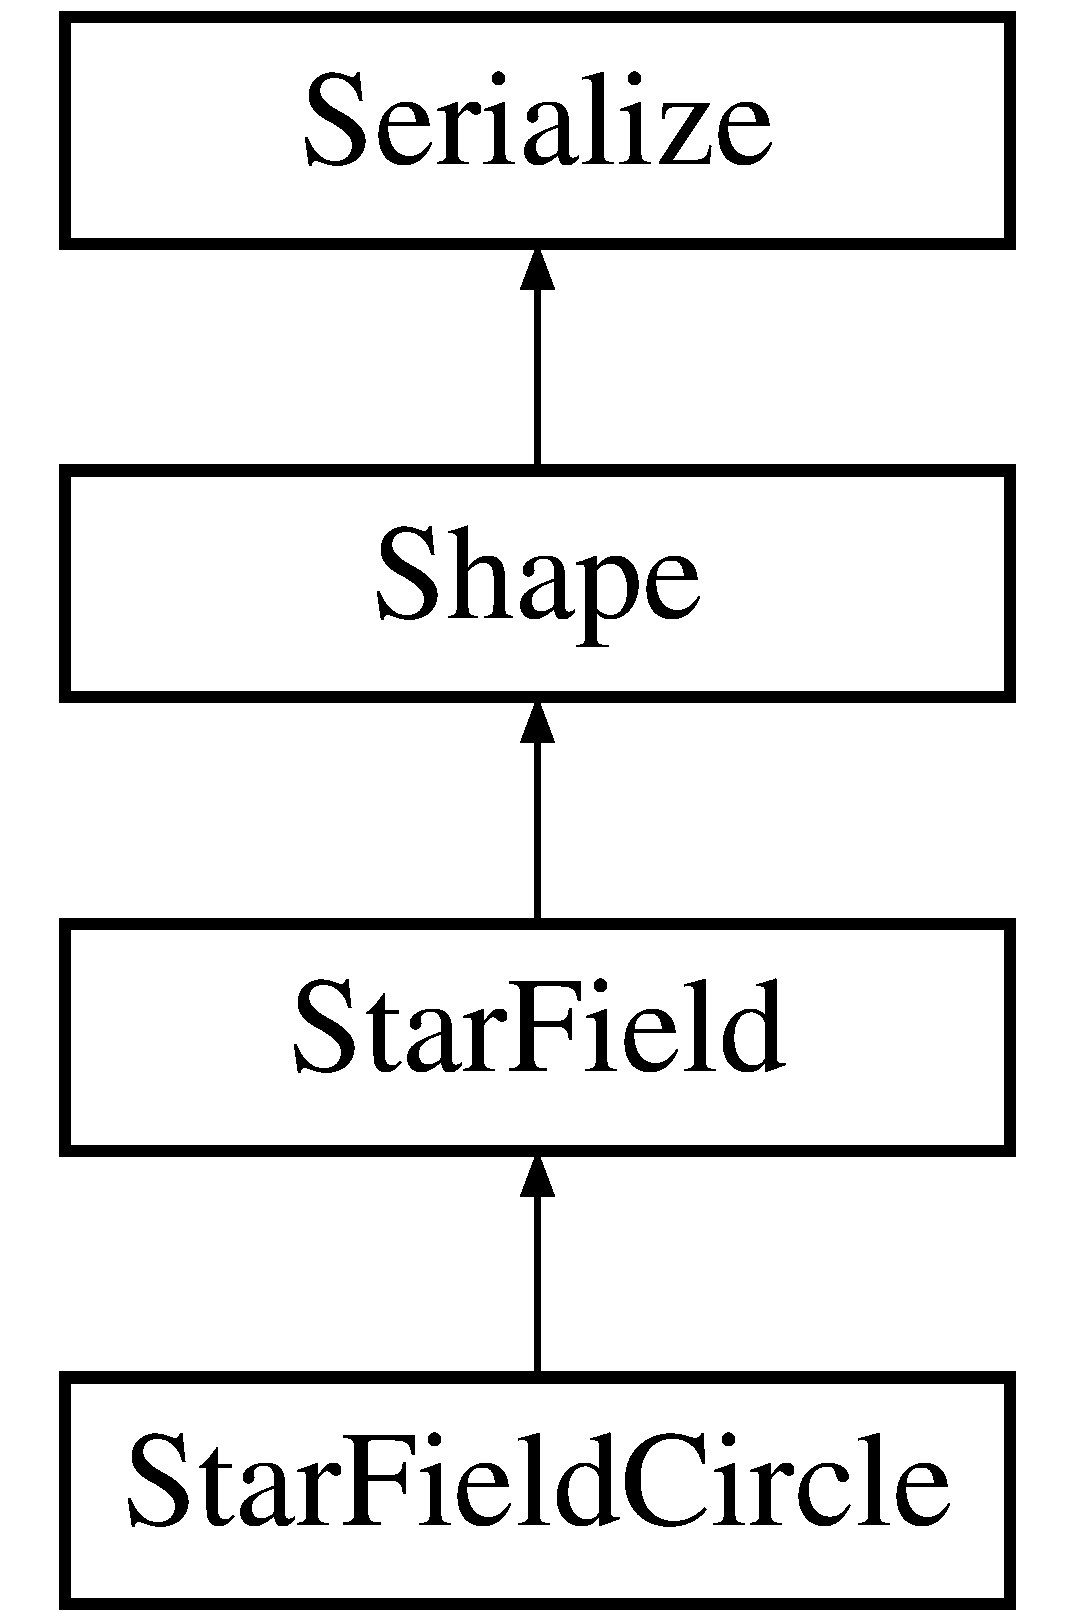
\includegraphics[height=4.000000cm]{classStarFieldCircle}
\end{center}
\end{figure}
\subsection*{Public Member Functions}
\begin{DoxyCompactItemize}
\item 
\hyperlink{classStarFieldCircle_a4b94a3f6c1c21271051f9bf3f8b42304}{Star\-Field\-Circle} ()
\item 
virtual \hyperlink{classStarFieldCircle_afea7e1add134916448c7bef6447e5f99}{$\sim$\-Star\-Field\-Circle} ()
\item 
void \hyperlink{classStarFieldCircle_af5d514f70b06701697786a9d7b09607c}{make\-Stars} (int nstars)
\item 
virtual void \hyperlink{classStarFieldCircle_af54e17032bb1ee195137b3585e7caea5}{move} (long double time)
\end{DoxyCompactItemize}
\subsection*{Additional Inherited Members}


\subsection{Constructor \& Destructor Documentation}
\hypertarget{classStarFieldCircle_a4b94a3f6c1c21271051f9bf3f8b42304}{\index{Star\-Field\-Circle@{Star\-Field\-Circle}!Star\-Field\-Circle@{Star\-Field\-Circle}}
\index{Star\-Field\-Circle@{Star\-Field\-Circle}!StarFieldCircle@{Star\-Field\-Circle}}
\subsubsection[{Star\-Field\-Circle}]{\setlength{\rightskip}{0pt plus 5cm}Star\-Field\-Circle\-::\-Star\-Field\-Circle (
\begin{DoxyParamCaption}
{}
\end{DoxyParamCaption}
)}}\label{classStarFieldCircle_a4b94a3f6c1c21271051f9bf3f8b42304}
\hypertarget{classStarFieldCircle_afea7e1add134916448c7bef6447e5f99}{\index{Star\-Field\-Circle@{Star\-Field\-Circle}!$\sim$\-Star\-Field\-Circle@{$\sim$\-Star\-Field\-Circle}}
\index{$\sim$\-Star\-Field\-Circle@{$\sim$\-Star\-Field\-Circle}!StarFieldCircle@{Star\-Field\-Circle}}
\subsubsection[{$\sim$\-Star\-Field\-Circle}]{\setlength{\rightskip}{0pt plus 5cm}Star\-Field\-Circle\-::$\sim$\-Star\-Field\-Circle (
\begin{DoxyParamCaption}
{}
\end{DoxyParamCaption}
)\hspace{0.3cm}{\ttfamily [virtual]}}}\label{classStarFieldCircle_afea7e1add134916448c7bef6447e5f99}


\subsection{Member Function Documentation}
\hypertarget{classStarFieldCircle_af5d514f70b06701697786a9d7b09607c}{\index{Star\-Field\-Circle@{Star\-Field\-Circle}!make\-Stars@{make\-Stars}}
\index{make\-Stars@{make\-Stars}!StarFieldCircle@{Star\-Field\-Circle}}
\subsubsection[{make\-Stars}]{\setlength{\rightskip}{0pt plus 5cm}void Star\-Field\-Circle\-::make\-Stars (
\begin{DoxyParamCaption}
\item[{int}]{nstars}
\end{DoxyParamCaption}
)\hspace{0.3cm}{\ttfamily [virtual]}}}\label{classStarFieldCircle_af5d514f70b06701697786a9d7b09607c}


Reimplemented from \hyperlink{classStarField_ae6b25b3827440dedf5836070205d4c6d}{Star\-Field}.

\hypertarget{classStarFieldCircle_af54e17032bb1ee195137b3585e7caea5}{\index{Star\-Field\-Circle@{Star\-Field\-Circle}!move@{move}}
\index{move@{move}!StarFieldCircle@{Star\-Field\-Circle}}
\subsubsection[{move}]{\setlength{\rightskip}{0pt plus 5cm}void Star\-Field\-Circle\-::move (
\begin{DoxyParamCaption}
\item[{long double}]{time}
\end{DoxyParamCaption}
)\hspace{0.3cm}{\ttfamily [virtual]}}}\label{classStarFieldCircle_af54e17032bb1ee195137b3585e7caea5}


Reimplemented from \hyperlink{classStarField_ac3e35d838577ed7610bdaf933ef5b99d}{Star\-Field}.



The documentation for this class was generated from the following files\-:\begin{DoxyCompactItemize}
\item 
/home/ruijan/sw/bmi5/bmi5/include/\-Shape/\hyperlink{starFieldCircle_8h}{star\-Field\-Circle.\-h}\item 
/home/ruijan/sw/bmi5/bmi5/src/\-Shape/\hyperlink{starFieldCircle_8cpp}{star\-Field\-Circle.\-cpp}\end{DoxyCompactItemize}

\hypertarget{structstarStruct}{\section{star\-Struct Struct Reference}
\label{structstarStruct}\index{star\-Struct@{star\-Struct}}
}


{\ttfamily \#include $<$star\-Field.\-h$>$}

\subsection*{Public Attributes}
\begin{DoxyCompactItemize}
\item 
float \hyperlink{structstarStruct_a76fdef62c69afe1a7014a757e0edb8f1}{position} \mbox{[}2\mbox{]}
\item 
unsigned int \hyperlink{structstarStruct_a9a62faf17da68e7cac83c2b898e21a90}{color}
\end{DoxyCompactItemize}


\subsection{Member Data Documentation}
\hypertarget{structstarStruct_a9a62faf17da68e7cac83c2b898e21a90}{\index{star\-Struct@{star\-Struct}!color@{color}}
\index{color@{color}!starStruct@{star\-Struct}}
\subsubsection[{color}]{\setlength{\rightskip}{0pt plus 5cm}unsigned int star\-Struct\-::color}}\label{structstarStruct_a9a62faf17da68e7cac83c2b898e21a90}
\hypertarget{structstarStruct_a76fdef62c69afe1a7014a757e0edb8f1}{\index{star\-Struct@{star\-Struct}!position@{position}}
\index{position@{position}!starStruct@{star\-Struct}}
\subsubsection[{position}]{\setlength{\rightskip}{0pt plus 5cm}float star\-Struct\-::position\mbox{[}2\mbox{]}}}\label{structstarStruct_a76fdef62c69afe1a7014a757e0edb8f1}


The documentation for this struct was generated from the following file\-:\begin{DoxyCompactItemize}
\item 
/home/ruijan/sw/bmi5/bmi5/include/\-Shape/\hyperlink{starField_8h}{star\-Field.\-h}\end{DoxyCompactItemize}

\hypertarget{classTdtUdpSerialize}{\section{Tdt\-Udp\-Serialize Class Reference}
\label{classTdtUdpSerialize}\index{Tdt\-Udp\-Serialize@{Tdt\-Udp\-Serialize}}
}


{\ttfamily \#include $<$tdt\-Udp\-Serialize.\-h$>$}

Inheritance diagram for Tdt\-Udp\-Serialize\-:\begin{figure}[H]
\begin{center}
\leavevmode
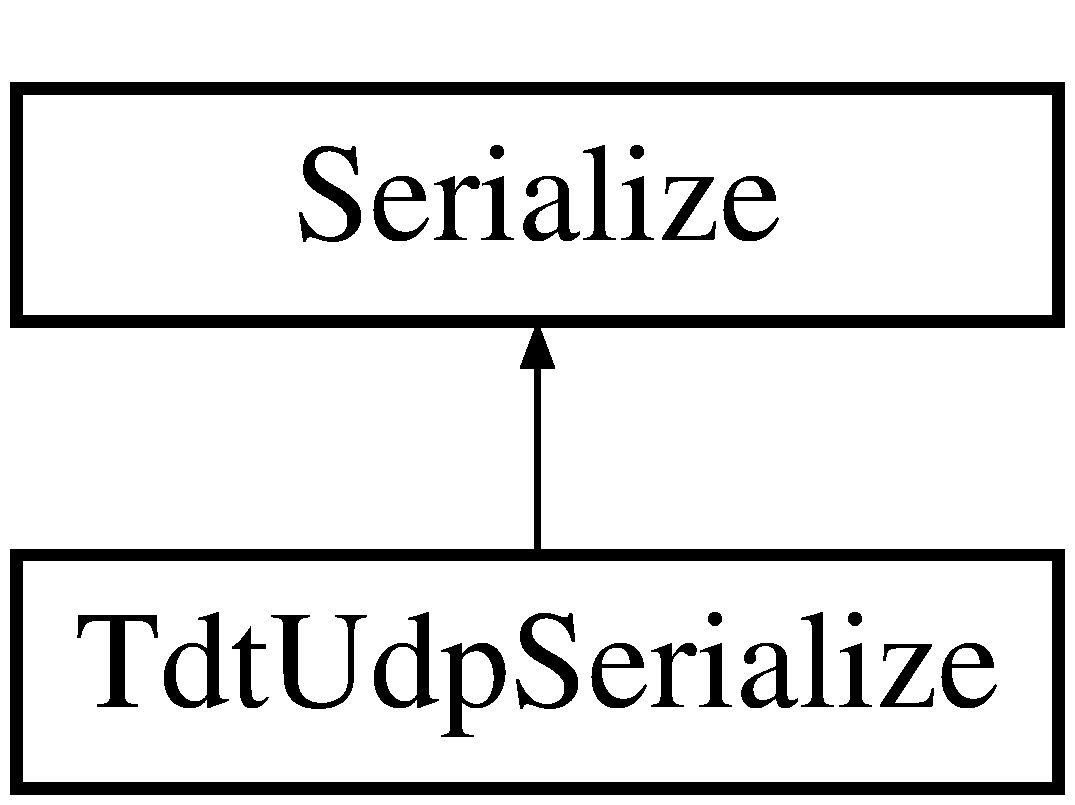
\includegraphics[height=2.000000cm]{classTdtUdpSerialize}
\end{center}
\end{figure}
\subsection*{Public Member Functions}
\begin{DoxyCompactItemize}
\item 
\hyperlink{classTdtUdpSerialize_a161b1f0f4e47f9d1e2cef6ebd14b0e95}{Tdt\-Udp\-Serialize} (int sock, int size)
\item 
\hyperlink{classTdtUdpSerialize_ae4b232bcd661aa79f445160acee8c631}{$\sim$\-Tdt\-Udp\-Serialize} ()
\item 
virtual bool \hyperlink{classTdtUdpSerialize_af90b9dd030658a60dd7221b68e47b0c1}{store} ()
\item 
virtual void \hyperlink{classTdtUdpSerialize_ac8510f3a23c5521f819c328d9e49bce7}{clear} ()
\item 
virtual int \hyperlink{classTdtUdpSerialize_a08a3fcd343162a03108e49e258a5faab}{nstored} ()
\item 
virtual string \hyperlink{classTdtUdpSerialize_aadd92c08f9323862f7f166a9e2cfaa83}{store\-Name} (int indx)
\item 
virtual int \hyperlink{classTdtUdpSerialize_a9dd4bd127aa84ce5aa4440a4e6f2f1ce}{get\-Store\-Class} (int indx)
\item 
virtual void \hyperlink{classTdtUdpSerialize_a1ef45e16bef8085e38796f0e94bc8333}{get\-Store\-Dims} (int indx, size\-\_\-t $\ast$dims)
\item 
virtual void $\ast$ \hyperlink{classTdtUdpSerialize_ae46b100495af52e51be07ed2df3e76d7}{get\-Store} (int indx, int k)
\item 
virtual int \hyperlink{classTdtUdpSerialize_a20d01c52f776c41002502949aae53896}{num\-Stores} ()
\item 
virtual double $\ast$ \hyperlink{classTdtUdpSerialize_ad22fb90570005daa6e8768c2f5dbb531}{mmap\-Read} (double $\ast$d)
\end{DoxyCompactItemize}
\subsection*{Public Attributes}
\begin{DoxyCompactItemize}
\item 
int \hyperlink{classTdtUdpSerialize_aa3fe3872eb26f196f0c01b077326a2b1}{m\-\_\-sock}
\item 
int \hyperlink{classTdtUdpSerialize_a80d8a9074ab3285377fd5e760713c5eb}{m\-\_\-size}
\item 
double \hyperlink{classTdtUdpSerialize_a5fde39b0fc2b63652da270b2986e4cf9}{m\-\_\-time}
\item 
vector$<$ double $>$ \hyperlink{classTdtUdpSerialize_a434574fb0198a3264abfdbdb28988848}{m\-\_\-last}
\item 
vector$<$ float $>$ \hyperlink{classTdtUdpSerialize_a4e644b3558110f98227c8888c5cd2ba1}{m\-\_\-stor}
\item 
vector$<$ double $>$ \hyperlink{classTdtUdpSerialize_abe092d1d2a2c134e75c8b4c228ff8426}{v\-\_\-time}
\item 
vector$<$ vector$<$ float $>$ $>$ \hyperlink{classTdtUdpSerialize_a16c2ac300794ee519b2d4a541202d1a1}{v\-\_\-stor}
\item 
float $\ast$ \hyperlink{classTdtUdpSerialize_a4eb083f9bac5c666d5221113723e7674}{m\-\_\-bs}
\end{DoxyCompactItemize}


\subsection{Constructor \& Destructor Documentation}
\hypertarget{classTdtUdpSerialize_a161b1f0f4e47f9d1e2cef6ebd14b0e95}{\index{Tdt\-Udp\-Serialize@{Tdt\-Udp\-Serialize}!Tdt\-Udp\-Serialize@{Tdt\-Udp\-Serialize}}
\index{Tdt\-Udp\-Serialize@{Tdt\-Udp\-Serialize}!TdtUdpSerialize@{Tdt\-Udp\-Serialize}}
\subsubsection[{Tdt\-Udp\-Serialize}]{\setlength{\rightskip}{0pt plus 5cm}Tdt\-Udp\-Serialize\-::\-Tdt\-Udp\-Serialize (
\begin{DoxyParamCaption}
\item[{int}]{sock, }
\item[{int}]{size}
\end{DoxyParamCaption}
)}}\label{classTdtUdpSerialize_a161b1f0f4e47f9d1e2cef6ebd14b0e95}
\hypertarget{classTdtUdpSerialize_ae4b232bcd661aa79f445160acee8c631}{\index{Tdt\-Udp\-Serialize@{Tdt\-Udp\-Serialize}!$\sim$\-Tdt\-Udp\-Serialize@{$\sim$\-Tdt\-Udp\-Serialize}}
\index{$\sim$\-Tdt\-Udp\-Serialize@{$\sim$\-Tdt\-Udp\-Serialize}!TdtUdpSerialize@{Tdt\-Udp\-Serialize}}
\subsubsection[{$\sim$\-Tdt\-Udp\-Serialize}]{\setlength{\rightskip}{0pt plus 5cm}Tdt\-Udp\-Serialize\-::$\sim$\-Tdt\-Udp\-Serialize (
\begin{DoxyParamCaption}
{}
\end{DoxyParamCaption}
)}}\label{classTdtUdpSerialize_ae4b232bcd661aa79f445160acee8c631}


\subsection{Member Function Documentation}
\hypertarget{classTdtUdpSerialize_ac8510f3a23c5521f819c328d9e49bce7}{\index{Tdt\-Udp\-Serialize@{Tdt\-Udp\-Serialize}!clear@{clear}}
\index{clear@{clear}!TdtUdpSerialize@{Tdt\-Udp\-Serialize}}
\subsubsection[{clear}]{\setlength{\rightskip}{0pt plus 5cm}void Tdt\-Udp\-Serialize\-::clear (
\begin{DoxyParamCaption}
{}
\end{DoxyParamCaption}
)\hspace{0.3cm}{\ttfamily [virtual]}}}\label{classTdtUdpSerialize_ac8510f3a23c5521f819c328d9e49bce7}


Reimplemented from \hyperlink{classSerialize_a11cbf006415c08d1891ab42e39a2aa1a}{Serialize}.

\hypertarget{classTdtUdpSerialize_ae46b100495af52e51be07ed2df3e76d7}{\index{Tdt\-Udp\-Serialize@{Tdt\-Udp\-Serialize}!get\-Store@{get\-Store}}
\index{get\-Store@{get\-Store}!TdtUdpSerialize@{Tdt\-Udp\-Serialize}}
\subsubsection[{get\-Store}]{\setlength{\rightskip}{0pt plus 5cm}void $\ast$ Tdt\-Udp\-Serialize\-::get\-Store (
\begin{DoxyParamCaption}
\item[{int}]{indx, }
\item[{int}]{k}
\end{DoxyParamCaption}
)\hspace{0.3cm}{\ttfamily [virtual]}}}\label{classTdtUdpSerialize_ae46b100495af52e51be07ed2df3e76d7}


Reimplemented from \hyperlink{classSerialize_a6e589d263cfdc0eb72e41687c58831f2}{Serialize}.

\hypertarget{classTdtUdpSerialize_a9dd4bd127aa84ce5aa4440a4e6f2f1ce}{\index{Tdt\-Udp\-Serialize@{Tdt\-Udp\-Serialize}!get\-Store\-Class@{get\-Store\-Class}}
\index{get\-Store\-Class@{get\-Store\-Class}!TdtUdpSerialize@{Tdt\-Udp\-Serialize}}
\subsubsection[{get\-Store\-Class}]{\setlength{\rightskip}{0pt plus 5cm}int Tdt\-Udp\-Serialize\-::get\-Store\-Class (
\begin{DoxyParamCaption}
\item[{int}]{indx}
\end{DoxyParamCaption}
)\hspace{0.3cm}{\ttfamily [virtual]}}}\label{classTdtUdpSerialize_a9dd4bd127aa84ce5aa4440a4e6f2f1ce}


Reimplemented from \hyperlink{classSerialize_a69954cc86d03b75b6b27511aec4aba43}{Serialize}.

\hypertarget{classTdtUdpSerialize_a1ef45e16bef8085e38796f0e94bc8333}{\index{Tdt\-Udp\-Serialize@{Tdt\-Udp\-Serialize}!get\-Store\-Dims@{get\-Store\-Dims}}
\index{get\-Store\-Dims@{get\-Store\-Dims}!TdtUdpSerialize@{Tdt\-Udp\-Serialize}}
\subsubsection[{get\-Store\-Dims}]{\setlength{\rightskip}{0pt plus 5cm}void Tdt\-Udp\-Serialize\-::get\-Store\-Dims (
\begin{DoxyParamCaption}
\item[{int}]{indx, }
\item[{size\-\_\-t $\ast$}]{dims}
\end{DoxyParamCaption}
)\hspace{0.3cm}{\ttfamily [virtual]}}}\label{classTdtUdpSerialize_a1ef45e16bef8085e38796f0e94bc8333}


Reimplemented from \hyperlink{classSerialize_a52034c5c17bc5e7e6c728b4e6c620c05}{Serialize}.

\hypertarget{classTdtUdpSerialize_ad22fb90570005daa6e8768c2f5dbb531}{\index{Tdt\-Udp\-Serialize@{Tdt\-Udp\-Serialize}!mmap\-Read@{mmap\-Read}}
\index{mmap\-Read@{mmap\-Read}!TdtUdpSerialize@{Tdt\-Udp\-Serialize}}
\subsubsection[{mmap\-Read}]{\setlength{\rightskip}{0pt plus 5cm}double $\ast$ Tdt\-Udp\-Serialize\-::mmap\-Read (
\begin{DoxyParamCaption}
\item[{double $\ast$}]{d}
\end{DoxyParamCaption}
)\hspace{0.3cm}{\ttfamily [virtual]}}}\label{classTdtUdpSerialize_ad22fb90570005daa6e8768c2f5dbb531}


Reimplemented from \hyperlink{classSerialize_a28b939242880e565a8906b30acd0f84c}{Serialize}.

\hypertarget{classTdtUdpSerialize_a08a3fcd343162a03108e49e258a5faab}{\index{Tdt\-Udp\-Serialize@{Tdt\-Udp\-Serialize}!nstored@{nstored}}
\index{nstored@{nstored}!TdtUdpSerialize@{Tdt\-Udp\-Serialize}}
\subsubsection[{nstored}]{\setlength{\rightskip}{0pt plus 5cm}int Tdt\-Udp\-Serialize\-::nstored (
\begin{DoxyParamCaption}
{}
\end{DoxyParamCaption}
)\hspace{0.3cm}{\ttfamily [virtual]}}}\label{classTdtUdpSerialize_a08a3fcd343162a03108e49e258a5faab}


Reimplemented from \hyperlink{classSerialize_a590b7308112b07581c03ba826ace50b4}{Serialize}.

\hypertarget{classTdtUdpSerialize_a20d01c52f776c41002502949aae53896}{\index{Tdt\-Udp\-Serialize@{Tdt\-Udp\-Serialize}!num\-Stores@{num\-Stores}}
\index{num\-Stores@{num\-Stores}!TdtUdpSerialize@{Tdt\-Udp\-Serialize}}
\subsubsection[{num\-Stores}]{\setlength{\rightskip}{0pt plus 5cm}int Tdt\-Udp\-Serialize\-::num\-Stores (
\begin{DoxyParamCaption}
{}
\end{DoxyParamCaption}
)\hspace{0.3cm}{\ttfamily [virtual]}}}\label{classTdtUdpSerialize_a20d01c52f776c41002502949aae53896}


Reimplemented from \hyperlink{classSerialize_a71bf2a906fd71477308a942d01490ab3}{Serialize}.

\hypertarget{classTdtUdpSerialize_af90b9dd030658a60dd7221b68e47b0c1}{\index{Tdt\-Udp\-Serialize@{Tdt\-Udp\-Serialize}!store@{store}}
\index{store@{store}!TdtUdpSerialize@{Tdt\-Udp\-Serialize}}
\subsubsection[{store}]{\setlength{\rightskip}{0pt plus 5cm}bool Tdt\-Udp\-Serialize\-::store (
\begin{DoxyParamCaption}
{}
\end{DoxyParamCaption}
)\hspace{0.3cm}{\ttfamily [virtual]}}}\label{classTdtUdpSerialize_af90b9dd030658a60dd7221b68e47b0c1}


Reimplemented from \hyperlink{classSerialize_a3cda20e84a530870a6115eaaf589f168}{Serialize}.

\hypertarget{classTdtUdpSerialize_aadd92c08f9323862f7f166a9e2cfaa83}{\index{Tdt\-Udp\-Serialize@{Tdt\-Udp\-Serialize}!store\-Name@{store\-Name}}
\index{store\-Name@{store\-Name}!TdtUdpSerialize@{Tdt\-Udp\-Serialize}}
\subsubsection[{store\-Name}]{\setlength{\rightskip}{0pt plus 5cm}string Tdt\-Udp\-Serialize\-::store\-Name (
\begin{DoxyParamCaption}
\item[{int}]{indx}
\end{DoxyParamCaption}
)\hspace{0.3cm}{\ttfamily [virtual]}}}\label{classTdtUdpSerialize_aadd92c08f9323862f7f166a9e2cfaa83}


Reimplemented from \hyperlink{classSerialize_ac94a76de6c9376e33b4c195d50ff0568}{Serialize}.



\subsection{Member Data Documentation}
\hypertarget{classTdtUdpSerialize_a4eb083f9bac5c666d5221113723e7674}{\index{Tdt\-Udp\-Serialize@{Tdt\-Udp\-Serialize}!m\-\_\-bs@{m\-\_\-bs}}
\index{m\-\_\-bs@{m\-\_\-bs}!TdtUdpSerialize@{Tdt\-Udp\-Serialize}}
\subsubsection[{m\-\_\-bs}]{\setlength{\rightskip}{0pt plus 5cm}float$\ast$ Tdt\-Udp\-Serialize\-::m\-\_\-bs}}\label{classTdtUdpSerialize_a4eb083f9bac5c666d5221113723e7674}
\hypertarget{classTdtUdpSerialize_a434574fb0198a3264abfdbdb28988848}{\index{Tdt\-Udp\-Serialize@{Tdt\-Udp\-Serialize}!m\-\_\-last@{m\-\_\-last}}
\index{m\-\_\-last@{m\-\_\-last}!TdtUdpSerialize@{Tdt\-Udp\-Serialize}}
\subsubsection[{m\-\_\-last}]{\setlength{\rightskip}{0pt plus 5cm}vector$<$double$>$ Tdt\-Udp\-Serialize\-::m\-\_\-last}}\label{classTdtUdpSerialize_a434574fb0198a3264abfdbdb28988848}
\hypertarget{classTdtUdpSerialize_a80d8a9074ab3285377fd5e760713c5eb}{\index{Tdt\-Udp\-Serialize@{Tdt\-Udp\-Serialize}!m\-\_\-size@{m\-\_\-size}}
\index{m\-\_\-size@{m\-\_\-size}!TdtUdpSerialize@{Tdt\-Udp\-Serialize}}
\subsubsection[{m\-\_\-size}]{\setlength{\rightskip}{0pt plus 5cm}int Tdt\-Udp\-Serialize\-::m\-\_\-size}}\label{classTdtUdpSerialize_a80d8a9074ab3285377fd5e760713c5eb}
\hypertarget{classTdtUdpSerialize_aa3fe3872eb26f196f0c01b077326a2b1}{\index{Tdt\-Udp\-Serialize@{Tdt\-Udp\-Serialize}!m\-\_\-sock@{m\-\_\-sock}}
\index{m\-\_\-sock@{m\-\_\-sock}!TdtUdpSerialize@{Tdt\-Udp\-Serialize}}
\subsubsection[{m\-\_\-sock}]{\setlength{\rightskip}{0pt plus 5cm}int Tdt\-Udp\-Serialize\-::m\-\_\-sock}}\label{classTdtUdpSerialize_aa3fe3872eb26f196f0c01b077326a2b1}
\hypertarget{classTdtUdpSerialize_a4e644b3558110f98227c8888c5cd2ba1}{\index{Tdt\-Udp\-Serialize@{Tdt\-Udp\-Serialize}!m\-\_\-stor@{m\-\_\-stor}}
\index{m\-\_\-stor@{m\-\_\-stor}!TdtUdpSerialize@{Tdt\-Udp\-Serialize}}
\subsubsection[{m\-\_\-stor}]{\setlength{\rightskip}{0pt plus 5cm}vector$<$float$>$ Tdt\-Udp\-Serialize\-::m\-\_\-stor}}\label{classTdtUdpSerialize_a4e644b3558110f98227c8888c5cd2ba1}
\hypertarget{classTdtUdpSerialize_a5fde39b0fc2b63652da270b2986e4cf9}{\index{Tdt\-Udp\-Serialize@{Tdt\-Udp\-Serialize}!m\-\_\-time@{m\-\_\-time}}
\index{m\-\_\-time@{m\-\_\-time}!TdtUdpSerialize@{Tdt\-Udp\-Serialize}}
\subsubsection[{m\-\_\-time}]{\setlength{\rightskip}{0pt plus 5cm}double Tdt\-Udp\-Serialize\-::m\-\_\-time}}\label{classTdtUdpSerialize_a5fde39b0fc2b63652da270b2986e4cf9}
\hypertarget{classTdtUdpSerialize_a16c2ac300794ee519b2d4a541202d1a1}{\index{Tdt\-Udp\-Serialize@{Tdt\-Udp\-Serialize}!v\-\_\-stor@{v\-\_\-stor}}
\index{v\-\_\-stor@{v\-\_\-stor}!TdtUdpSerialize@{Tdt\-Udp\-Serialize}}
\subsubsection[{v\-\_\-stor}]{\setlength{\rightskip}{0pt plus 5cm}vector$<$vector$<$float$>$ $>$ Tdt\-Udp\-Serialize\-::v\-\_\-stor}}\label{classTdtUdpSerialize_a16c2ac300794ee519b2d4a541202d1a1}
\hypertarget{classTdtUdpSerialize_abe092d1d2a2c134e75c8b4c228ff8426}{\index{Tdt\-Udp\-Serialize@{Tdt\-Udp\-Serialize}!v\-\_\-time@{v\-\_\-time}}
\index{v\-\_\-time@{v\-\_\-time}!TdtUdpSerialize@{Tdt\-Udp\-Serialize}}
\subsubsection[{v\-\_\-time}]{\setlength{\rightskip}{0pt plus 5cm}vector$<$double$>$ Tdt\-Udp\-Serialize\-::v\-\_\-time}}\label{classTdtUdpSerialize_abe092d1d2a2c134e75c8b4c228ff8426}


The documentation for this class was generated from the following files\-:\begin{DoxyCompactItemize}
\item 
/home/ruijan/sw/bmi5/bmi5/include/\-Serialize/\hyperlink{tdtUdpSerialize_8h}{tdt\-Udp\-Serialize.\-h}\item 
/home/ruijan/sw/bmi5/bmi5/src/\-Serialize/\hyperlink{tdtUdpSerialize_8cpp}{tdt\-Udp\-Serialize.\-cpp}\end{DoxyCompactItemize}

\hypertarget{classTimeSerialize}{\section{Time\-Serialize Class Reference}
\label{classTimeSerialize}\index{Time\-Serialize@{Time\-Serialize}}
}


{\ttfamily \#include $<$time\-Serialize.\-h$>$}

Inheritance diagram for Time\-Serialize\-:\begin{figure}[H]
\begin{center}
\leavevmode
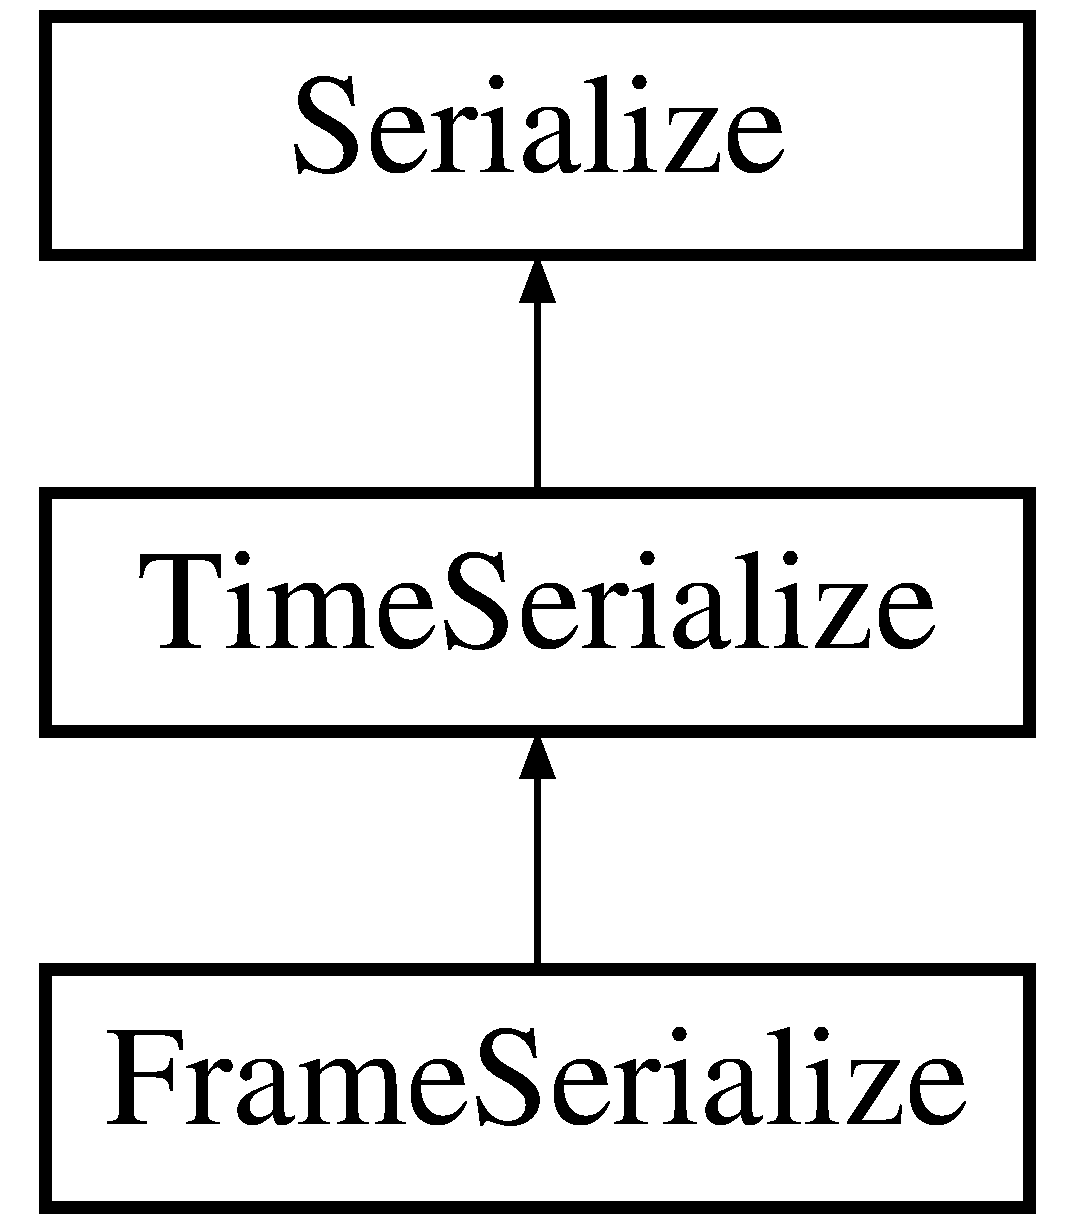
\includegraphics[height=3.000000cm]{classTimeSerialize}
\end{center}
\end{figure}
\subsection*{Public Member Functions}
\begin{DoxyCompactItemize}
\item 
\hyperlink{classTimeSerialize_ae7880f4e7d36aebd66c5efa14622439c}{Time\-Serialize} ()
\item 
\hyperlink{classTimeSerialize_a8134ab931baed7946fe9b8a63e696361}{$\sim$\-Time\-Serialize} ()
\item 
virtual bool \hyperlink{classTimeSerialize_a5fa3f8491cf69cafb608ed06d16b744b}{store} ()
\item 
virtual void \hyperlink{classTimeSerialize_a2dc0323aaec9735cec278fce2ab70779}{clear} ()
\item 
virtual int \hyperlink{classTimeSerialize_a8decf0dd155f7c185d5ed4a96ad8df6e}{nstored} ()
\item 
virtual string \hyperlink{classTimeSerialize_aee9a422ba150037d03eaac84f98bb74a}{store\-Name} (int indx)
\item 
virtual int \hyperlink{classTimeSerialize_aabe62de35575d2e543c1b6a60adee905}{get\-Store\-Class} (int indx)
\item 
virtual void \hyperlink{classTimeSerialize_a012cef4eb5d7766296987d57dcd7b6d1}{get\-Store\-Dims} (int, size\-\_\-t $\ast$dims)
\item 
virtual void $\ast$ \hyperlink{classTimeSerialize_aca830871918f9acf615366df5e1eeb11}{get\-Store} (int indx, int i)
\item 
virtual int \hyperlink{classTimeSerialize_af36ff5a97baec0656b91373b72796a5f}{num\-Stores} ()
\item 
virtual double $\ast$ \hyperlink{classTimeSerialize_ac7a17bf484eb4e7970532b6a1ed65325}{mmap\-Read} (double $\ast$d)
\end{DoxyCompactItemize}
\subsection*{Public Attributes}
\begin{DoxyCompactItemize}
\item 
vector$<$ double $>$ \hyperlink{classTimeSerialize_acc179754062d5bee1d77a19ecbc948d6}{v\-\_\-time}
\item 
vector$<$ double $>$ \hyperlink{classTimeSerialize_affc36f2cdf92fd934e8c77fe15954ec9}{v\-\_\-ticks}
\item 
vector$<$ int $>$ \hyperlink{classTimeSerialize_ae215c04e400b72cc80d3e91552335dee}{v\-\_\-frame}
\end{DoxyCompactItemize}


\subsection{Constructor \& Destructor Documentation}
\hypertarget{classTimeSerialize_ae7880f4e7d36aebd66c5efa14622439c}{\index{Time\-Serialize@{Time\-Serialize}!Time\-Serialize@{Time\-Serialize}}
\index{Time\-Serialize@{Time\-Serialize}!TimeSerialize@{Time\-Serialize}}
\subsubsection[{Time\-Serialize}]{\setlength{\rightskip}{0pt plus 5cm}Time\-Serialize\-::\-Time\-Serialize (
\begin{DoxyParamCaption}
{}
\end{DoxyParamCaption}
)}}\label{classTimeSerialize_ae7880f4e7d36aebd66c5efa14622439c}
\hypertarget{classTimeSerialize_a8134ab931baed7946fe9b8a63e696361}{\index{Time\-Serialize@{Time\-Serialize}!$\sim$\-Time\-Serialize@{$\sim$\-Time\-Serialize}}
\index{$\sim$\-Time\-Serialize@{$\sim$\-Time\-Serialize}!TimeSerialize@{Time\-Serialize}}
\subsubsection[{$\sim$\-Time\-Serialize}]{\setlength{\rightskip}{0pt plus 5cm}Time\-Serialize\-::$\sim$\-Time\-Serialize (
\begin{DoxyParamCaption}
{}
\end{DoxyParamCaption}
)}}\label{classTimeSerialize_a8134ab931baed7946fe9b8a63e696361}


\subsection{Member Function Documentation}
\hypertarget{classTimeSerialize_a2dc0323aaec9735cec278fce2ab70779}{\index{Time\-Serialize@{Time\-Serialize}!clear@{clear}}
\index{clear@{clear}!TimeSerialize@{Time\-Serialize}}
\subsubsection[{clear}]{\setlength{\rightskip}{0pt plus 5cm}void Time\-Serialize\-::clear (
\begin{DoxyParamCaption}
{}
\end{DoxyParamCaption}
)\hspace{0.3cm}{\ttfamily [virtual]}}}\label{classTimeSerialize_a2dc0323aaec9735cec278fce2ab70779}


Reimplemented from \hyperlink{classSerialize_a11cbf006415c08d1891ab42e39a2aa1a}{Serialize}.

\hypertarget{classTimeSerialize_aca830871918f9acf615366df5e1eeb11}{\index{Time\-Serialize@{Time\-Serialize}!get\-Store@{get\-Store}}
\index{get\-Store@{get\-Store}!TimeSerialize@{Time\-Serialize}}
\subsubsection[{get\-Store}]{\setlength{\rightskip}{0pt plus 5cm}void $\ast$ Time\-Serialize\-::get\-Store (
\begin{DoxyParamCaption}
\item[{int}]{indx, }
\item[{int}]{i}
\end{DoxyParamCaption}
)\hspace{0.3cm}{\ttfamily [virtual]}}}\label{classTimeSerialize_aca830871918f9acf615366df5e1eeb11}


Reimplemented from \hyperlink{classSerialize_a6e589d263cfdc0eb72e41687c58831f2}{Serialize}.

\hypertarget{classTimeSerialize_aabe62de35575d2e543c1b6a60adee905}{\index{Time\-Serialize@{Time\-Serialize}!get\-Store\-Class@{get\-Store\-Class}}
\index{get\-Store\-Class@{get\-Store\-Class}!TimeSerialize@{Time\-Serialize}}
\subsubsection[{get\-Store\-Class}]{\setlength{\rightskip}{0pt plus 5cm}int Time\-Serialize\-::get\-Store\-Class (
\begin{DoxyParamCaption}
\item[{int}]{indx}
\end{DoxyParamCaption}
)\hspace{0.3cm}{\ttfamily [virtual]}}}\label{classTimeSerialize_aabe62de35575d2e543c1b6a60adee905}


Reimplemented from \hyperlink{classSerialize_a69954cc86d03b75b6b27511aec4aba43}{Serialize}.

\hypertarget{classTimeSerialize_a012cef4eb5d7766296987d57dcd7b6d1}{\index{Time\-Serialize@{Time\-Serialize}!get\-Store\-Dims@{get\-Store\-Dims}}
\index{get\-Store\-Dims@{get\-Store\-Dims}!TimeSerialize@{Time\-Serialize}}
\subsubsection[{get\-Store\-Dims}]{\setlength{\rightskip}{0pt plus 5cm}void Time\-Serialize\-::get\-Store\-Dims (
\begin{DoxyParamCaption}
\item[{int}]{, }
\item[{size\-\_\-t $\ast$}]{dims}
\end{DoxyParamCaption}
)\hspace{0.3cm}{\ttfamily [virtual]}}}\label{classTimeSerialize_a012cef4eb5d7766296987d57dcd7b6d1}


Reimplemented from \hyperlink{classSerialize_a52034c5c17bc5e7e6c728b4e6c620c05}{Serialize}.

\hypertarget{classTimeSerialize_ac7a17bf484eb4e7970532b6a1ed65325}{\index{Time\-Serialize@{Time\-Serialize}!mmap\-Read@{mmap\-Read}}
\index{mmap\-Read@{mmap\-Read}!TimeSerialize@{Time\-Serialize}}
\subsubsection[{mmap\-Read}]{\setlength{\rightskip}{0pt plus 5cm}double $\ast$ Time\-Serialize\-::mmap\-Read (
\begin{DoxyParamCaption}
\item[{double $\ast$}]{d}
\end{DoxyParamCaption}
)\hspace{0.3cm}{\ttfamily [virtual]}}}\label{classTimeSerialize_ac7a17bf484eb4e7970532b6a1ed65325}


Reimplemented from \hyperlink{classSerialize_a28b939242880e565a8906b30acd0f84c}{Serialize}.



Reimplemented in \hyperlink{classFrameSerialize_a9d775f9c379f0444a82cd309bba9e9b1}{Frame\-Serialize}.

\hypertarget{classTimeSerialize_a8decf0dd155f7c185d5ed4a96ad8df6e}{\index{Time\-Serialize@{Time\-Serialize}!nstored@{nstored}}
\index{nstored@{nstored}!TimeSerialize@{Time\-Serialize}}
\subsubsection[{nstored}]{\setlength{\rightskip}{0pt plus 5cm}int Time\-Serialize\-::nstored (
\begin{DoxyParamCaption}
{}
\end{DoxyParamCaption}
)\hspace{0.3cm}{\ttfamily [virtual]}}}\label{classTimeSerialize_a8decf0dd155f7c185d5ed4a96ad8df6e}


Reimplemented from \hyperlink{classSerialize_a590b7308112b07581c03ba826ace50b4}{Serialize}.

\hypertarget{classTimeSerialize_af36ff5a97baec0656b91373b72796a5f}{\index{Time\-Serialize@{Time\-Serialize}!num\-Stores@{num\-Stores}}
\index{num\-Stores@{num\-Stores}!TimeSerialize@{Time\-Serialize}}
\subsubsection[{num\-Stores}]{\setlength{\rightskip}{0pt plus 5cm}int Time\-Serialize\-::num\-Stores (
\begin{DoxyParamCaption}
{}
\end{DoxyParamCaption}
)\hspace{0.3cm}{\ttfamily [virtual]}}}\label{classTimeSerialize_af36ff5a97baec0656b91373b72796a5f}


Reimplemented from \hyperlink{classSerialize_a71bf2a906fd71477308a942d01490ab3}{Serialize}.

\hypertarget{classTimeSerialize_a5fa3f8491cf69cafb608ed06d16b744b}{\index{Time\-Serialize@{Time\-Serialize}!store@{store}}
\index{store@{store}!TimeSerialize@{Time\-Serialize}}
\subsubsection[{store}]{\setlength{\rightskip}{0pt plus 5cm}bool Time\-Serialize\-::store (
\begin{DoxyParamCaption}
{}
\end{DoxyParamCaption}
)\hspace{0.3cm}{\ttfamily [virtual]}}}\label{classTimeSerialize_a5fa3f8491cf69cafb608ed06d16b744b}


Reimplemented from \hyperlink{classSerialize_a3cda20e84a530870a6115eaaf589f168}{Serialize}.



Reimplemented in \hyperlink{classFrameSerialize_a5c2bbf78b071f73554611b82ad395573}{Frame\-Serialize}.

\hypertarget{classTimeSerialize_aee9a422ba150037d03eaac84f98bb74a}{\index{Time\-Serialize@{Time\-Serialize}!store\-Name@{store\-Name}}
\index{store\-Name@{store\-Name}!TimeSerialize@{Time\-Serialize}}
\subsubsection[{store\-Name}]{\setlength{\rightskip}{0pt plus 5cm}string Time\-Serialize\-::store\-Name (
\begin{DoxyParamCaption}
\item[{int}]{indx}
\end{DoxyParamCaption}
)\hspace{0.3cm}{\ttfamily [virtual]}}}\label{classTimeSerialize_aee9a422ba150037d03eaac84f98bb74a}


Reimplemented from \hyperlink{classSerialize_ac94a76de6c9376e33b4c195d50ff0568}{Serialize}.



\subsection{Member Data Documentation}
\hypertarget{classTimeSerialize_ae215c04e400b72cc80d3e91552335dee}{\index{Time\-Serialize@{Time\-Serialize}!v\-\_\-frame@{v\-\_\-frame}}
\index{v\-\_\-frame@{v\-\_\-frame}!TimeSerialize@{Time\-Serialize}}
\subsubsection[{v\-\_\-frame}]{\setlength{\rightskip}{0pt plus 5cm}vector$<$int$>$ Time\-Serialize\-::v\-\_\-frame}}\label{classTimeSerialize_ae215c04e400b72cc80d3e91552335dee}
\hypertarget{classTimeSerialize_affc36f2cdf92fd934e8c77fe15954ec9}{\index{Time\-Serialize@{Time\-Serialize}!v\-\_\-ticks@{v\-\_\-ticks}}
\index{v\-\_\-ticks@{v\-\_\-ticks}!TimeSerialize@{Time\-Serialize}}
\subsubsection[{v\-\_\-ticks}]{\setlength{\rightskip}{0pt plus 5cm}vector$<$double$>$ Time\-Serialize\-::v\-\_\-ticks}}\label{classTimeSerialize_affc36f2cdf92fd934e8c77fe15954ec9}
\hypertarget{classTimeSerialize_acc179754062d5bee1d77a19ecbc948d6}{\index{Time\-Serialize@{Time\-Serialize}!v\-\_\-time@{v\-\_\-time}}
\index{v\-\_\-time@{v\-\_\-time}!TimeSerialize@{Time\-Serialize}}
\subsubsection[{v\-\_\-time}]{\setlength{\rightskip}{0pt plus 5cm}vector$<$double$>$ Time\-Serialize\-::v\-\_\-time}}\label{classTimeSerialize_acc179754062d5bee1d77a19ecbc948d6}


The documentation for this class was generated from the following files\-:\begin{DoxyCompactItemize}
\item 
/home/ruijan/sw/bmi5/bmi5/include/\-Serialize/\hyperlink{timeSerialize_8h}{time\-Serialize.\-h}\item 
/home/ruijan/sw/bmi5/bmi5/src/\-Serialize/\hyperlink{timeSerialize_8cpp}{time\-Serialize.\-cpp}\end{DoxyCompactItemize}

\hypertarget{classToneSerialize}{\section{Tone\-Serialize Class Reference}
\label{classToneSerialize}\index{Tone\-Serialize@{Tone\-Serialize}}
}


{\ttfamily \#include $<$tone\-Serialize.\-h$>$}

Inheritance diagram for Tone\-Serialize\-:\begin{figure}[H]
\begin{center}
\leavevmode
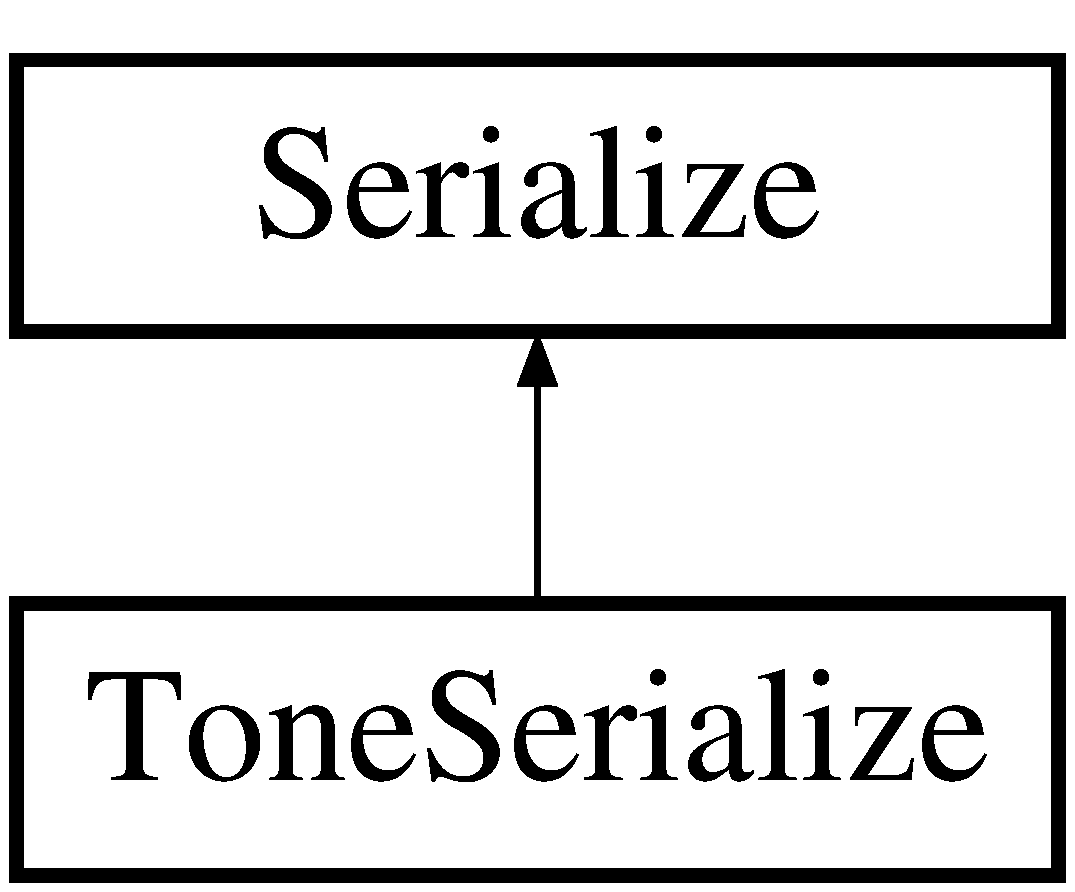
\includegraphics[height=2.000000cm]{classToneSerialize}
\end{center}
\end{figure}
\subsection*{Public Member Functions}
\begin{DoxyCompactItemize}
\item 
\hyperlink{classToneSerialize_aa7a4f5168cfa0f247718c26be93a29b8}{Tone\-Serialize} ()
\item 
\hyperlink{classToneSerialize_a05907704997b3c3456cef49dc5d68ad8}{$\sim$\-Tone\-Serialize} ()
\item 
virtual bool \hyperlink{classToneSerialize_ab67181fa3c51dded04a2d8b4fc55edb4}{store} ()
\item 
virtual void \hyperlink{classToneSerialize_a1670e9459e05b63f1b6fff4d6ff13099}{clear} ()
\item 
virtual int \hyperlink{classToneSerialize_a6a5a872eb9e1a282c0de2221c777c144}{nstored} ()
\item 
virtual string \hyperlink{classToneSerialize_a4ae952e04b0a89ba3d5a8cb82460b064}{store\-Name} (int indx)
\item 
virtual int \hyperlink{classToneSerialize_a651a5292dabf70de6f562695ca034d8d}{get\-Store\-Class} (int indx)
\item 
virtual void \hyperlink{classToneSerialize_a3756f8357f284843aeaa5c56f98ff5db}{get\-Store\-Dims} (int, size\-\_\-t $\ast$dims)
\item 
virtual void $\ast$ \hyperlink{classToneSerialize_a6999157d41af65a3b7e8ea101972fd4e}{get\-Store} (int indx, int i)
\item 
virtual int \hyperlink{classToneSerialize_a85f4bff56b0f43466079c2ff289aa03a}{num\-Stores} ()
\item 
virtual double $\ast$ \hyperlink{classToneSerialize_adaf612569b11204b02fc3393b780f75e}{mmap\-Read} (double $\ast$d)
\end{DoxyCompactItemize}
\subsection*{Public Attributes}
\begin{DoxyCompactItemize}
\item 
double \hyperlink{classToneSerialize_aa17b08f9fbad9ad86eb39f6b87843948}{m\-\_\-time}
\end{DoxyCompactItemize}
\subsection*{Private Attributes}
\begin{DoxyCompactItemize}
\item 
vector$<$ double $>$ \hyperlink{classToneSerialize_a2b10ad240255d0094337d0c3078e5e10}{v\-\_\-time}
\item 
vector$<$ float $>$ \hyperlink{classToneSerialize_a5888cb2c1c082334173c99c5cb4cbbc0}{v\-\_\-freq}
\item 
vector$<$ float $>$ \hyperlink{classToneSerialize_acab1f55a7935a7a20358ef96785d9576}{v\-\_\-pan}
\item 
vector$<$ float $>$ \hyperlink{classToneSerialize_ab6e8afad24a81b6dcfc3c6970fe289eb}{v\-\_\-scale}
\item 
vector$<$ float $>$ \hyperlink{classToneSerialize_a01cf609e28a438fc1effb03c656b33d6}{v\-\_\-duration}
\item 
vector$<$ char $>$ \hyperlink{classToneSerialize_a9313ff97557d382476944defa90f6a8e}{v\-\_\-play}
\end{DoxyCompactItemize}


\subsection{Constructor \& Destructor Documentation}
\hypertarget{classToneSerialize_aa7a4f5168cfa0f247718c26be93a29b8}{\index{Tone\-Serialize@{Tone\-Serialize}!Tone\-Serialize@{Tone\-Serialize}}
\index{Tone\-Serialize@{Tone\-Serialize}!ToneSerialize@{Tone\-Serialize}}
\subsubsection[{Tone\-Serialize}]{\setlength{\rightskip}{0pt plus 5cm}Tone\-Serialize\-::\-Tone\-Serialize (
\begin{DoxyParamCaption}
{}
\end{DoxyParamCaption}
)}}\label{classToneSerialize_aa7a4f5168cfa0f247718c26be93a29b8}
\hypertarget{classToneSerialize_a05907704997b3c3456cef49dc5d68ad8}{\index{Tone\-Serialize@{Tone\-Serialize}!$\sim$\-Tone\-Serialize@{$\sim$\-Tone\-Serialize}}
\index{$\sim$\-Tone\-Serialize@{$\sim$\-Tone\-Serialize}!ToneSerialize@{Tone\-Serialize}}
\subsubsection[{$\sim$\-Tone\-Serialize}]{\setlength{\rightskip}{0pt plus 5cm}Tone\-Serialize\-::$\sim$\-Tone\-Serialize (
\begin{DoxyParamCaption}
{}
\end{DoxyParamCaption}
)}}\label{classToneSerialize_a05907704997b3c3456cef49dc5d68ad8}


\subsection{Member Function Documentation}
\hypertarget{classToneSerialize_a1670e9459e05b63f1b6fff4d6ff13099}{\index{Tone\-Serialize@{Tone\-Serialize}!clear@{clear}}
\index{clear@{clear}!ToneSerialize@{Tone\-Serialize}}
\subsubsection[{clear}]{\setlength{\rightskip}{0pt plus 5cm}void Tone\-Serialize\-::clear (
\begin{DoxyParamCaption}
{}
\end{DoxyParamCaption}
)\hspace{0.3cm}{\ttfamily [virtual]}}}\label{classToneSerialize_a1670e9459e05b63f1b6fff4d6ff13099}


Reimplemented from \hyperlink{classSerialize_a11cbf006415c08d1891ab42e39a2aa1a}{Serialize}.

\hypertarget{classToneSerialize_a6999157d41af65a3b7e8ea101972fd4e}{\index{Tone\-Serialize@{Tone\-Serialize}!get\-Store@{get\-Store}}
\index{get\-Store@{get\-Store}!ToneSerialize@{Tone\-Serialize}}
\subsubsection[{get\-Store}]{\setlength{\rightskip}{0pt plus 5cm}void $\ast$ Tone\-Serialize\-::get\-Store (
\begin{DoxyParamCaption}
\item[{int}]{indx, }
\item[{int}]{i}
\end{DoxyParamCaption}
)\hspace{0.3cm}{\ttfamily [virtual]}}}\label{classToneSerialize_a6999157d41af65a3b7e8ea101972fd4e}


Reimplemented from \hyperlink{classSerialize_a6e589d263cfdc0eb72e41687c58831f2}{Serialize}.

\hypertarget{classToneSerialize_a651a5292dabf70de6f562695ca034d8d}{\index{Tone\-Serialize@{Tone\-Serialize}!get\-Store\-Class@{get\-Store\-Class}}
\index{get\-Store\-Class@{get\-Store\-Class}!ToneSerialize@{Tone\-Serialize}}
\subsubsection[{get\-Store\-Class}]{\setlength{\rightskip}{0pt plus 5cm}int Tone\-Serialize\-::get\-Store\-Class (
\begin{DoxyParamCaption}
\item[{int}]{indx}
\end{DoxyParamCaption}
)\hspace{0.3cm}{\ttfamily [virtual]}}}\label{classToneSerialize_a651a5292dabf70de6f562695ca034d8d}


Reimplemented from \hyperlink{classSerialize_a69954cc86d03b75b6b27511aec4aba43}{Serialize}.

\hypertarget{classToneSerialize_a3756f8357f284843aeaa5c56f98ff5db}{\index{Tone\-Serialize@{Tone\-Serialize}!get\-Store\-Dims@{get\-Store\-Dims}}
\index{get\-Store\-Dims@{get\-Store\-Dims}!ToneSerialize@{Tone\-Serialize}}
\subsubsection[{get\-Store\-Dims}]{\setlength{\rightskip}{0pt plus 5cm}void Tone\-Serialize\-::get\-Store\-Dims (
\begin{DoxyParamCaption}
\item[{int}]{, }
\item[{size\-\_\-t $\ast$}]{dims}
\end{DoxyParamCaption}
)\hspace{0.3cm}{\ttfamily [virtual]}}}\label{classToneSerialize_a3756f8357f284843aeaa5c56f98ff5db}


Reimplemented from \hyperlink{classSerialize_a52034c5c17bc5e7e6c728b4e6c620c05}{Serialize}.

\hypertarget{classToneSerialize_adaf612569b11204b02fc3393b780f75e}{\index{Tone\-Serialize@{Tone\-Serialize}!mmap\-Read@{mmap\-Read}}
\index{mmap\-Read@{mmap\-Read}!ToneSerialize@{Tone\-Serialize}}
\subsubsection[{mmap\-Read}]{\setlength{\rightskip}{0pt plus 5cm}double $\ast$ Tone\-Serialize\-::mmap\-Read (
\begin{DoxyParamCaption}
\item[{double $\ast$}]{d}
\end{DoxyParamCaption}
)\hspace{0.3cm}{\ttfamily [virtual]}}}\label{classToneSerialize_adaf612569b11204b02fc3393b780f75e}


Reimplemented from \hyperlink{classSerialize_a28b939242880e565a8906b30acd0f84c}{Serialize}.

\hypertarget{classToneSerialize_a6a5a872eb9e1a282c0de2221c777c144}{\index{Tone\-Serialize@{Tone\-Serialize}!nstored@{nstored}}
\index{nstored@{nstored}!ToneSerialize@{Tone\-Serialize}}
\subsubsection[{nstored}]{\setlength{\rightskip}{0pt plus 5cm}int Tone\-Serialize\-::nstored (
\begin{DoxyParamCaption}
{}
\end{DoxyParamCaption}
)\hspace{0.3cm}{\ttfamily [virtual]}}}\label{classToneSerialize_a6a5a872eb9e1a282c0de2221c777c144}


Reimplemented from \hyperlink{classSerialize_a590b7308112b07581c03ba826ace50b4}{Serialize}.

\hypertarget{classToneSerialize_a85f4bff56b0f43466079c2ff289aa03a}{\index{Tone\-Serialize@{Tone\-Serialize}!num\-Stores@{num\-Stores}}
\index{num\-Stores@{num\-Stores}!ToneSerialize@{Tone\-Serialize}}
\subsubsection[{num\-Stores}]{\setlength{\rightskip}{0pt plus 5cm}int Tone\-Serialize\-::num\-Stores (
\begin{DoxyParamCaption}
{}
\end{DoxyParamCaption}
)\hspace{0.3cm}{\ttfamily [virtual]}}}\label{classToneSerialize_a85f4bff56b0f43466079c2ff289aa03a}


Reimplemented from \hyperlink{classSerialize_a71bf2a906fd71477308a942d01490ab3}{Serialize}.

\hypertarget{classToneSerialize_ab67181fa3c51dded04a2d8b4fc55edb4}{\index{Tone\-Serialize@{Tone\-Serialize}!store@{store}}
\index{store@{store}!ToneSerialize@{Tone\-Serialize}}
\subsubsection[{store}]{\setlength{\rightskip}{0pt plus 5cm}bool Tone\-Serialize\-::store (
\begin{DoxyParamCaption}
{}
\end{DoxyParamCaption}
)\hspace{0.3cm}{\ttfamily [virtual]}}}\label{classToneSerialize_ab67181fa3c51dded04a2d8b4fc55edb4}


Reimplemented from \hyperlink{classSerialize_a3cda20e84a530870a6115eaaf589f168}{Serialize}.

\hypertarget{classToneSerialize_a4ae952e04b0a89ba3d5a8cb82460b064}{\index{Tone\-Serialize@{Tone\-Serialize}!store\-Name@{store\-Name}}
\index{store\-Name@{store\-Name}!ToneSerialize@{Tone\-Serialize}}
\subsubsection[{store\-Name}]{\setlength{\rightskip}{0pt plus 5cm}string Tone\-Serialize\-::store\-Name (
\begin{DoxyParamCaption}
\item[{int}]{indx}
\end{DoxyParamCaption}
)\hspace{0.3cm}{\ttfamily [virtual]}}}\label{classToneSerialize_a4ae952e04b0a89ba3d5a8cb82460b064}


Reimplemented from \hyperlink{classSerialize_ac94a76de6c9376e33b4c195d50ff0568}{Serialize}.



\subsection{Member Data Documentation}
\hypertarget{classToneSerialize_aa17b08f9fbad9ad86eb39f6b87843948}{\index{Tone\-Serialize@{Tone\-Serialize}!m\-\_\-time@{m\-\_\-time}}
\index{m\-\_\-time@{m\-\_\-time}!ToneSerialize@{Tone\-Serialize}}
\subsubsection[{m\-\_\-time}]{\setlength{\rightskip}{0pt plus 5cm}double Tone\-Serialize\-::m\-\_\-time}}\label{classToneSerialize_aa17b08f9fbad9ad86eb39f6b87843948}
\hypertarget{classToneSerialize_a01cf609e28a438fc1effb03c656b33d6}{\index{Tone\-Serialize@{Tone\-Serialize}!v\-\_\-duration@{v\-\_\-duration}}
\index{v\-\_\-duration@{v\-\_\-duration}!ToneSerialize@{Tone\-Serialize}}
\subsubsection[{v\-\_\-duration}]{\setlength{\rightskip}{0pt plus 5cm}vector$<$float$>$ Tone\-Serialize\-::v\-\_\-duration\hspace{0.3cm}{\ttfamily [private]}}}\label{classToneSerialize_a01cf609e28a438fc1effb03c656b33d6}
\hypertarget{classToneSerialize_a5888cb2c1c082334173c99c5cb4cbbc0}{\index{Tone\-Serialize@{Tone\-Serialize}!v\-\_\-freq@{v\-\_\-freq}}
\index{v\-\_\-freq@{v\-\_\-freq}!ToneSerialize@{Tone\-Serialize}}
\subsubsection[{v\-\_\-freq}]{\setlength{\rightskip}{0pt plus 5cm}vector$<$float$>$ Tone\-Serialize\-::v\-\_\-freq\hspace{0.3cm}{\ttfamily [private]}}}\label{classToneSerialize_a5888cb2c1c082334173c99c5cb4cbbc0}
\hypertarget{classToneSerialize_acab1f55a7935a7a20358ef96785d9576}{\index{Tone\-Serialize@{Tone\-Serialize}!v\-\_\-pan@{v\-\_\-pan}}
\index{v\-\_\-pan@{v\-\_\-pan}!ToneSerialize@{Tone\-Serialize}}
\subsubsection[{v\-\_\-pan}]{\setlength{\rightskip}{0pt plus 5cm}vector$<$float$>$ Tone\-Serialize\-::v\-\_\-pan\hspace{0.3cm}{\ttfamily [private]}}}\label{classToneSerialize_acab1f55a7935a7a20358ef96785d9576}
\hypertarget{classToneSerialize_a9313ff97557d382476944defa90f6a8e}{\index{Tone\-Serialize@{Tone\-Serialize}!v\-\_\-play@{v\-\_\-play}}
\index{v\-\_\-play@{v\-\_\-play}!ToneSerialize@{Tone\-Serialize}}
\subsubsection[{v\-\_\-play}]{\setlength{\rightskip}{0pt plus 5cm}vector$<$char$>$ Tone\-Serialize\-::v\-\_\-play\hspace{0.3cm}{\ttfamily [private]}}}\label{classToneSerialize_a9313ff97557d382476944defa90f6a8e}
\hypertarget{classToneSerialize_ab6e8afad24a81b6dcfc3c6970fe289eb}{\index{Tone\-Serialize@{Tone\-Serialize}!v\-\_\-scale@{v\-\_\-scale}}
\index{v\-\_\-scale@{v\-\_\-scale}!ToneSerialize@{Tone\-Serialize}}
\subsubsection[{v\-\_\-scale}]{\setlength{\rightskip}{0pt plus 5cm}vector$<$float$>$ Tone\-Serialize\-::v\-\_\-scale\hspace{0.3cm}{\ttfamily [private]}}}\label{classToneSerialize_ab6e8afad24a81b6dcfc3c6970fe289eb}
\hypertarget{classToneSerialize_a2b10ad240255d0094337d0c3078e5e10}{\index{Tone\-Serialize@{Tone\-Serialize}!v\-\_\-time@{v\-\_\-time}}
\index{v\-\_\-time@{v\-\_\-time}!ToneSerialize@{Tone\-Serialize}}
\subsubsection[{v\-\_\-time}]{\setlength{\rightskip}{0pt plus 5cm}vector$<$double$>$ Tone\-Serialize\-::v\-\_\-time\hspace{0.3cm}{\ttfamily [private]}}}\label{classToneSerialize_a2b10ad240255d0094337d0c3078e5e10}


The documentation for this class was generated from the following files\-:\begin{DoxyCompactItemize}
\item 
/home/ruijan/sw/bmi5/bmi5/include/\-Serialize/\hyperlink{toneSerialize_8h}{tone\-Serialize.\-h}\item 
/home/ruijan/sw/bmi5/bmi5/src/\-Serialize/\hyperlink{toneSerialize_8cpp}{tone\-Serialize.\-cpp}\end{DoxyCompactItemize}

\hypertarget{structU6__CALIBRATION__INFORMATION}{\section{U6\-\_\-\-C\-A\-L\-I\-B\-R\-A\-T\-I\-O\-N\-\_\-\-I\-N\-F\-O\-R\-M\-A\-T\-I\-O\-N Struct Reference}
\label{structU6__CALIBRATION__INFORMATION}\index{U6\-\_\-\-C\-A\-L\-I\-B\-R\-A\-T\-I\-O\-N\-\_\-\-I\-N\-F\-O\-R\-M\-A\-T\-I\-O\-N@{U6\-\_\-\-C\-A\-L\-I\-B\-R\-A\-T\-I\-O\-N\-\_\-\-I\-N\-F\-O\-R\-M\-A\-T\-I\-O\-N}}
}


{\ttfamily \#include $<$u6.\-h$>$}

\subsection*{Public Attributes}
\begin{DoxyCompactItemize}
\item 
\hyperlink{u6_8h_adde6aaee8457bee49c2a92621fe22b79}{uint8} \hyperlink{structU6__CALIBRATION__INFORMATION_a8ca95218c797bfb20202d9cb32ca5a70}{prod\-I\-D}
\item 
\hyperlink{u6_8h_adde6aaee8457bee49c2a92621fe22b79}{uint8} \hyperlink{structU6__CALIBRATION__INFORMATION_a2a621c3dc6e444fc947e536d7910c81c}{hi\-Res}
\item 
double \hyperlink{structU6__CALIBRATION__INFORMATION_a8f1f630eec649ae0fc9a946787a3cfdf}{cc\-Constants} \mbox{[}40\mbox{]}
\end{DoxyCompactItemize}


\subsection{Member Data Documentation}
\hypertarget{structU6__CALIBRATION__INFORMATION_a8f1f630eec649ae0fc9a946787a3cfdf}{\index{U6\-\_\-\-C\-A\-L\-I\-B\-R\-A\-T\-I\-O\-N\-\_\-\-I\-N\-F\-O\-R\-M\-A\-T\-I\-O\-N@{U6\-\_\-\-C\-A\-L\-I\-B\-R\-A\-T\-I\-O\-N\-\_\-\-I\-N\-F\-O\-R\-M\-A\-T\-I\-O\-N}!cc\-Constants@{cc\-Constants}}
\index{cc\-Constants@{cc\-Constants}!U6_CALIBRATION_INFORMATION@{U6\-\_\-\-C\-A\-L\-I\-B\-R\-A\-T\-I\-O\-N\-\_\-\-I\-N\-F\-O\-R\-M\-A\-T\-I\-O\-N}}
\subsubsection[{cc\-Constants}]{\setlength{\rightskip}{0pt plus 5cm}double U6\-\_\-\-C\-A\-L\-I\-B\-R\-A\-T\-I\-O\-N\-\_\-\-I\-N\-F\-O\-R\-M\-A\-T\-I\-O\-N\-::cc\-Constants\mbox{[}40\mbox{]}}}\label{structU6__CALIBRATION__INFORMATION_a8f1f630eec649ae0fc9a946787a3cfdf}
\hypertarget{structU6__CALIBRATION__INFORMATION_a2a621c3dc6e444fc947e536d7910c81c}{\index{U6\-\_\-\-C\-A\-L\-I\-B\-R\-A\-T\-I\-O\-N\-\_\-\-I\-N\-F\-O\-R\-M\-A\-T\-I\-O\-N@{U6\-\_\-\-C\-A\-L\-I\-B\-R\-A\-T\-I\-O\-N\-\_\-\-I\-N\-F\-O\-R\-M\-A\-T\-I\-O\-N}!hi\-Res@{hi\-Res}}
\index{hi\-Res@{hi\-Res}!U6_CALIBRATION_INFORMATION@{U6\-\_\-\-C\-A\-L\-I\-B\-R\-A\-T\-I\-O\-N\-\_\-\-I\-N\-F\-O\-R\-M\-A\-T\-I\-O\-N}}
\subsubsection[{hi\-Res}]{\setlength{\rightskip}{0pt plus 5cm}{\bf uint8} U6\-\_\-\-C\-A\-L\-I\-B\-R\-A\-T\-I\-O\-N\-\_\-\-I\-N\-F\-O\-R\-M\-A\-T\-I\-O\-N\-::hi\-Res}}\label{structU6__CALIBRATION__INFORMATION_a2a621c3dc6e444fc947e536d7910c81c}
\hypertarget{structU6__CALIBRATION__INFORMATION_a8ca95218c797bfb20202d9cb32ca5a70}{\index{U6\-\_\-\-C\-A\-L\-I\-B\-R\-A\-T\-I\-O\-N\-\_\-\-I\-N\-F\-O\-R\-M\-A\-T\-I\-O\-N@{U6\-\_\-\-C\-A\-L\-I\-B\-R\-A\-T\-I\-O\-N\-\_\-\-I\-N\-F\-O\-R\-M\-A\-T\-I\-O\-N}!prod\-I\-D@{prod\-I\-D}}
\index{prod\-I\-D@{prod\-I\-D}!U6_CALIBRATION_INFORMATION@{U6\-\_\-\-C\-A\-L\-I\-B\-R\-A\-T\-I\-O\-N\-\_\-\-I\-N\-F\-O\-R\-M\-A\-T\-I\-O\-N}}
\subsubsection[{prod\-I\-D}]{\setlength{\rightskip}{0pt plus 5cm}{\bf uint8} U6\-\_\-\-C\-A\-L\-I\-B\-R\-A\-T\-I\-O\-N\-\_\-\-I\-N\-F\-O\-R\-M\-A\-T\-I\-O\-N\-::prod\-I\-D}}\label{structU6__CALIBRATION__INFORMATION_a8ca95218c797bfb20202d9cb32ca5a70}


The documentation for this struct was generated from the following file\-:\begin{DoxyCompactItemize}
\item 
/home/ruijan/sw/bmi5/bmi5/include/\hyperlink{u6_8h}{u6.\-h}\end{DoxyCompactItemize}

\hypertarget{structU6__TDAC__CALIBRATION__INFORMATION}{\section{U6\-\_\-\-T\-D\-A\-C\-\_\-\-C\-A\-L\-I\-B\-R\-A\-T\-I\-O\-N\-\_\-\-I\-N\-F\-O\-R\-M\-A\-T\-I\-O\-N Struct Reference}
\label{structU6__TDAC__CALIBRATION__INFORMATION}\index{U6\-\_\-\-T\-D\-A\-C\-\_\-\-C\-A\-L\-I\-B\-R\-A\-T\-I\-O\-N\-\_\-\-I\-N\-F\-O\-R\-M\-A\-T\-I\-O\-N@{U6\-\_\-\-T\-D\-A\-C\-\_\-\-C\-A\-L\-I\-B\-R\-A\-T\-I\-O\-N\-\_\-\-I\-N\-F\-O\-R\-M\-A\-T\-I\-O\-N}}
}


{\ttfamily \#include $<$u6.\-h$>$}

\subsection*{Public Attributes}
\begin{DoxyCompactItemize}
\item 
\hyperlink{u6_8h_adde6aaee8457bee49c2a92621fe22b79}{uint8} \hyperlink{structU6__TDAC__CALIBRATION__INFORMATION_a712075dcac43ecc629ba0908bb2e59f9}{prod\-I\-D}
\item 
double \hyperlink{structU6__TDAC__CALIBRATION__INFORMATION_a7aab6102304d21a37162d00db515cec6}{cc\-Constants} \mbox{[}4\mbox{]}
\end{DoxyCompactItemize}


\subsection{Member Data Documentation}
\hypertarget{structU6__TDAC__CALIBRATION__INFORMATION_a7aab6102304d21a37162d00db515cec6}{\index{U6\-\_\-\-T\-D\-A\-C\-\_\-\-C\-A\-L\-I\-B\-R\-A\-T\-I\-O\-N\-\_\-\-I\-N\-F\-O\-R\-M\-A\-T\-I\-O\-N@{U6\-\_\-\-T\-D\-A\-C\-\_\-\-C\-A\-L\-I\-B\-R\-A\-T\-I\-O\-N\-\_\-\-I\-N\-F\-O\-R\-M\-A\-T\-I\-O\-N}!cc\-Constants@{cc\-Constants}}
\index{cc\-Constants@{cc\-Constants}!U6_TDAC_CALIBRATION_INFORMATION@{U6\-\_\-\-T\-D\-A\-C\-\_\-\-C\-A\-L\-I\-B\-R\-A\-T\-I\-O\-N\-\_\-\-I\-N\-F\-O\-R\-M\-A\-T\-I\-O\-N}}
\subsubsection[{cc\-Constants}]{\setlength{\rightskip}{0pt plus 5cm}double U6\-\_\-\-T\-D\-A\-C\-\_\-\-C\-A\-L\-I\-B\-R\-A\-T\-I\-O\-N\-\_\-\-I\-N\-F\-O\-R\-M\-A\-T\-I\-O\-N\-::cc\-Constants\mbox{[}4\mbox{]}}}\label{structU6__TDAC__CALIBRATION__INFORMATION_a7aab6102304d21a37162d00db515cec6}
\hypertarget{structU6__TDAC__CALIBRATION__INFORMATION_a712075dcac43ecc629ba0908bb2e59f9}{\index{U6\-\_\-\-T\-D\-A\-C\-\_\-\-C\-A\-L\-I\-B\-R\-A\-T\-I\-O\-N\-\_\-\-I\-N\-F\-O\-R\-M\-A\-T\-I\-O\-N@{U6\-\_\-\-T\-D\-A\-C\-\_\-\-C\-A\-L\-I\-B\-R\-A\-T\-I\-O\-N\-\_\-\-I\-N\-F\-O\-R\-M\-A\-T\-I\-O\-N}!prod\-I\-D@{prod\-I\-D}}
\index{prod\-I\-D@{prod\-I\-D}!U6_TDAC_CALIBRATION_INFORMATION@{U6\-\_\-\-T\-D\-A\-C\-\_\-\-C\-A\-L\-I\-B\-R\-A\-T\-I\-O\-N\-\_\-\-I\-N\-F\-O\-R\-M\-A\-T\-I\-O\-N}}
\subsubsection[{prod\-I\-D}]{\setlength{\rightskip}{0pt plus 5cm}{\bf uint8} U6\-\_\-\-T\-D\-A\-C\-\_\-\-C\-A\-L\-I\-B\-R\-A\-T\-I\-O\-N\-\_\-\-I\-N\-F\-O\-R\-M\-A\-T\-I\-O\-N\-::prod\-I\-D}}\label{structU6__TDAC__CALIBRATION__INFORMATION_a712075dcac43ecc629ba0908bb2e59f9}


The documentation for this struct was generated from the following file\-:\begin{DoxyCompactItemize}
\item 
/home/ruijan/sw/bmi5/bmi5/include/\hyperlink{u6_8h}{u6.\-h}\end{DoxyCompactItemize}

\hypertarget{classVectorSerialize}{\section{Vector\-Serialize$<$ T $>$ Class Template Reference}
\label{classVectorSerialize}\index{Vector\-Serialize$<$ T $>$@{Vector\-Serialize$<$ T $>$}}
}


{\ttfamily \#include $<$vector\-Serialize.\-h$>$}

Inheritance diagram for Vector\-Serialize$<$ T $>$\-:\begin{figure}[H]
\begin{center}
\leavevmode
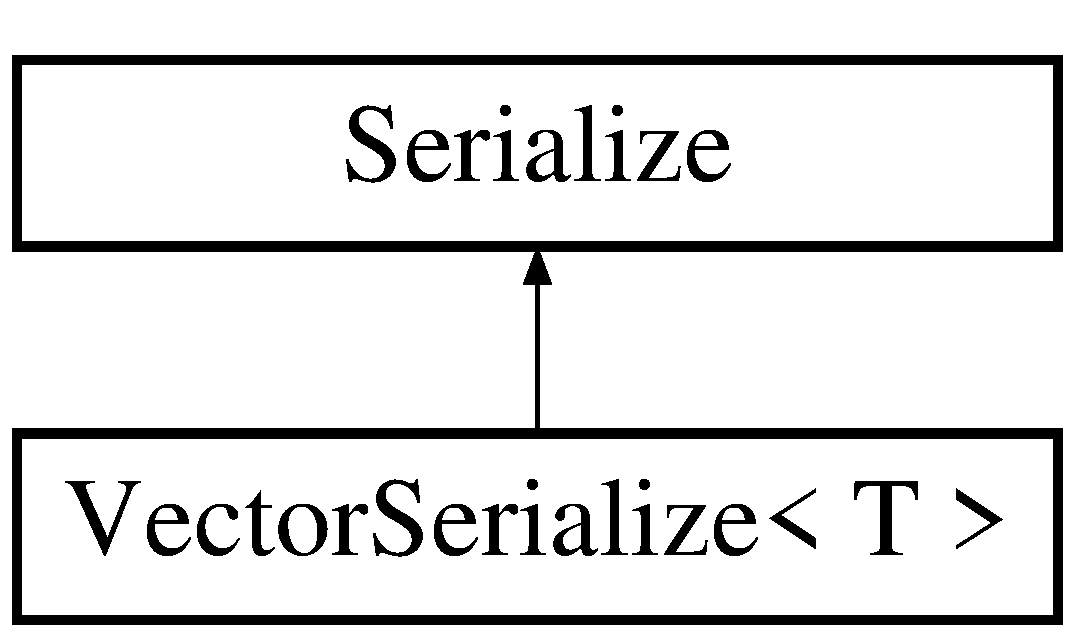
\includegraphics[height=2.000000cm]{classVectorSerialize}
\end{center}
\end{figure}
\subsection*{Public Member Functions}
\begin{DoxyCompactItemize}
\item 
\hyperlink{classVectorSerialize_a60c3584a75eb413096821a82b9c4324f}{Vector\-Serialize} (int size, int matiotype)
\item 
\hyperlink{classVectorSerialize_a34d822f6145f446eb01aae2c1f4634cb}{$\sim$\-Vector\-Serialize} ()
\item 
virtual bool \hyperlink{classVectorSerialize_afd6b6dc8768969dae5f27f46eeab83e6}{store} ()
\item 
virtual void \hyperlink{classVectorSerialize_ae94606fef7aec9ade8142d3cd56449ab}{clear} ()
\item 
virtual int \hyperlink{classVectorSerialize_a97c0db5a4da6c14c9c053092cc89e2bd}{nstored} ()
\item 
virtual string \hyperlink{classVectorSerialize_a929f94f68d0a99c61308520a679ae1a2}{store\-Name} (int indx)
\item 
virtual int \hyperlink{classVectorSerialize_a03d8454fff77942e63cd1764f1013f2d}{get\-Store\-Class} (int indx)
\item 
virtual void \hyperlink{classVectorSerialize_aa22f90d57d8802670716f4b859d6b069}{get\-Store\-Dims} (int indx, size\-\_\-t $\ast$dims)
\item 
virtual void $\ast$ \hyperlink{classVectorSerialize_a08f1412b11fb7b034da21c5ec131489b}{get\-Store} (int indx, int k)
\item 
virtual int \hyperlink{classVectorSerialize_a15226c69bda0fff870f20026f8681d80}{num\-Stores} ()
\item 
virtual double $\ast$ \hyperlink{classVectorSerialize_a087c30b15095d1b230705e42123eb3db}{mmap\-Read} (double $\ast$d)
\end{DoxyCompactItemize}
\subsection*{Public Attributes}
\begin{DoxyCompactItemize}
\item 
int \hyperlink{classVectorSerialize_a27a2e15a8897856a754e6cfeabd79c37}{m\-\_\-size}
\item 
int \hyperlink{classVectorSerialize_ae3e04f4e93664fdefc8091048ec92153}{m\-\_\-type}
\item 
double \hyperlink{classVectorSerialize_ab30720112fe2e2ae893a40f9f06d1fe8}{m\-\_\-time}
\item 
vector$<$ T $>$ \hyperlink{classVectorSerialize_a14f4a4320d206dfe1c631b95eccac441}{m\-\_\-stor}
\item 
vector$<$ double $>$ \hyperlink{classVectorSerialize_a43ce9711f370fa70f243971d66e50d70}{v\-\_\-time}
\item 
vector$<$ vector$<$ T $>$ $>$ \hyperlink{classVectorSerialize_aa092678fb5228aa59774c637755e65c4}{v\-\_\-stor}
\item 
T $\ast$ \hyperlink{classVectorSerialize_a19b31e3bdca1c74b3255948dc88328a7}{m\-\_\-bs}
\end{DoxyCompactItemize}


\subsection{Constructor \& Destructor Documentation}
\hypertarget{classVectorSerialize_a60c3584a75eb413096821a82b9c4324f}{\index{Vector\-Serialize@{Vector\-Serialize}!Vector\-Serialize@{Vector\-Serialize}}
\index{Vector\-Serialize@{Vector\-Serialize}!VectorSerialize@{Vector\-Serialize}}
\subsubsection[{Vector\-Serialize}]{\setlength{\rightskip}{0pt plus 5cm}template$<$class T $>$ {\bf Vector\-Serialize}$<$ T $>$\-::{\bf Vector\-Serialize} (
\begin{DoxyParamCaption}
\item[{int}]{size, }
\item[{int}]{matiotype}
\end{DoxyParamCaption}
)}}\label{classVectorSerialize_a60c3584a75eb413096821a82b9c4324f}
\hypertarget{classVectorSerialize_a34d822f6145f446eb01aae2c1f4634cb}{\index{Vector\-Serialize@{Vector\-Serialize}!$\sim$\-Vector\-Serialize@{$\sim$\-Vector\-Serialize}}
\index{$\sim$\-Vector\-Serialize@{$\sim$\-Vector\-Serialize}!VectorSerialize@{Vector\-Serialize}}
\subsubsection[{$\sim$\-Vector\-Serialize}]{\setlength{\rightskip}{0pt plus 5cm}template$<$class T $>$ {\bf Vector\-Serialize}$<$ T $>$\-::$\sim${\bf Vector\-Serialize} (
\begin{DoxyParamCaption}
{}
\end{DoxyParamCaption}
)}}\label{classVectorSerialize_a34d822f6145f446eb01aae2c1f4634cb}


\subsection{Member Function Documentation}
\hypertarget{classVectorSerialize_ae94606fef7aec9ade8142d3cd56449ab}{\index{Vector\-Serialize@{Vector\-Serialize}!clear@{clear}}
\index{clear@{clear}!VectorSerialize@{Vector\-Serialize}}
\subsubsection[{clear}]{\setlength{\rightskip}{0pt plus 5cm}template$<$class T $>$ void {\bf Vector\-Serialize}$<$ T $>$\-::clear (
\begin{DoxyParamCaption}
{}
\end{DoxyParamCaption}
)\hspace{0.3cm}{\ttfamily [virtual]}}}\label{classVectorSerialize_ae94606fef7aec9ade8142d3cd56449ab}


Reimplemented from \hyperlink{classSerialize_a11cbf006415c08d1891ab42e39a2aa1a}{Serialize}.



Reimplemented in \hyperlink{classDisplayText_a0c7a7a5200482ea4817f6c550dc7dea9}{Display\-Text}.

\hypertarget{classVectorSerialize_a08f1412b11fb7b034da21c5ec131489b}{\index{Vector\-Serialize@{Vector\-Serialize}!get\-Store@{get\-Store}}
\index{get\-Store@{get\-Store}!VectorSerialize@{Vector\-Serialize}}
\subsubsection[{get\-Store}]{\setlength{\rightskip}{0pt plus 5cm}template$<$class T $>$ void $\ast$ {\bf Vector\-Serialize}$<$ T $>$\-::get\-Store (
\begin{DoxyParamCaption}
\item[{int}]{indx, }
\item[{int}]{k}
\end{DoxyParamCaption}
)\hspace{0.3cm}{\ttfamily [virtual]}}}\label{classVectorSerialize_a08f1412b11fb7b034da21c5ec131489b}


Reimplemented from \hyperlink{classSerialize_a6e589d263cfdc0eb72e41687c58831f2}{Serialize}.



Reimplemented in \hyperlink{classDisplayText_aea5003c9c461955ec3c9a3a4b4fc2c25}{Display\-Text}.

\hypertarget{classVectorSerialize_a03d8454fff77942e63cd1764f1013f2d}{\index{Vector\-Serialize@{Vector\-Serialize}!get\-Store\-Class@{get\-Store\-Class}}
\index{get\-Store\-Class@{get\-Store\-Class}!VectorSerialize@{Vector\-Serialize}}
\subsubsection[{get\-Store\-Class}]{\setlength{\rightskip}{0pt plus 5cm}template$<$class T $>$ int {\bf Vector\-Serialize}$<$ T $>$\-::get\-Store\-Class (
\begin{DoxyParamCaption}
\item[{int}]{indx}
\end{DoxyParamCaption}
)\hspace{0.3cm}{\ttfamily [virtual]}}}\label{classVectorSerialize_a03d8454fff77942e63cd1764f1013f2d}


Reimplemented from \hyperlink{classSerialize_a69954cc86d03b75b6b27511aec4aba43}{Serialize}.



Reimplemented in \hyperlink{classDisplayText_aaa8ccb67b152d79505e5acc8448770ed}{Display\-Text}.

\hypertarget{classVectorSerialize_aa22f90d57d8802670716f4b859d6b069}{\index{Vector\-Serialize@{Vector\-Serialize}!get\-Store\-Dims@{get\-Store\-Dims}}
\index{get\-Store\-Dims@{get\-Store\-Dims}!VectorSerialize@{Vector\-Serialize}}
\subsubsection[{get\-Store\-Dims}]{\setlength{\rightskip}{0pt plus 5cm}template$<$class T $>$ void {\bf Vector\-Serialize}$<$ T $>$\-::get\-Store\-Dims (
\begin{DoxyParamCaption}
\item[{int}]{indx, }
\item[{size\-\_\-t $\ast$}]{dims}
\end{DoxyParamCaption}
)\hspace{0.3cm}{\ttfamily [virtual]}}}\label{classVectorSerialize_aa22f90d57d8802670716f4b859d6b069}


Reimplemented from \hyperlink{classSerialize_a52034c5c17bc5e7e6c728b4e6c620c05}{Serialize}.



Reimplemented in \hyperlink{classDisplayText_a81a37dd4e0fa54265843db620c371d02}{Display\-Text}.

\hypertarget{classVectorSerialize_a087c30b15095d1b230705e42123eb3db}{\index{Vector\-Serialize@{Vector\-Serialize}!mmap\-Read@{mmap\-Read}}
\index{mmap\-Read@{mmap\-Read}!VectorSerialize@{Vector\-Serialize}}
\subsubsection[{mmap\-Read}]{\setlength{\rightskip}{0pt plus 5cm}template$<$class T $>$ double $\ast$ {\bf Vector\-Serialize}$<$ T $>$\-::mmap\-Read (
\begin{DoxyParamCaption}
\item[{double $\ast$}]{d}
\end{DoxyParamCaption}
)\hspace{0.3cm}{\ttfamily [virtual]}}}\label{classVectorSerialize_a087c30b15095d1b230705e42123eb3db}


Reimplemented from \hyperlink{classSerialize_a28b939242880e565a8906b30acd0f84c}{Serialize}.



Reimplemented in \hyperlink{classDisplayText_ae5f08045997631736d8400ad3662fe5b}{Display\-Text}, \hyperlink{classLabjackSerializeAIN_a5b64792931481c509eb0c2bb86dbc99a}{Labjack\-Serialize\-A\-I\-N}, \hyperlink{classLabjackSerializeDOUT_a8936d25baa4652bb431b02ccb60489be}{Labjack\-Serialize\-D\-O\-U\-T}, and \hyperlink{classMouseSerialize_ab919e98d4daf8a068fc68741a4a4dcb7}{Mouse\-Serialize}.

\hypertarget{classVectorSerialize_a97c0db5a4da6c14c9c053092cc89e2bd}{\index{Vector\-Serialize@{Vector\-Serialize}!nstored@{nstored}}
\index{nstored@{nstored}!VectorSerialize@{Vector\-Serialize}}
\subsubsection[{nstored}]{\setlength{\rightskip}{0pt plus 5cm}template$<$class T $>$ int {\bf Vector\-Serialize}$<$ T $>$\-::nstored (
\begin{DoxyParamCaption}
{}
\end{DoxyParamCaption}
)\hspace{0.3cm}{\ttfamily [virtual]}}}\label{classVectorSerialize_a97c0db5a4da6c14c9c053092cc89e2bd}


Reimplemented from \hyperlink{classSerialize_a590b7308112b07581c03ba826ace50b4}{Serialize}.

\hypertarget{classVectorSerialize_a15226c69bda0fff870f20026f8681d80}{\index{Vector\-Serialize@{Vector\-Serialize}!num\-Stores@{num\-Stores}}
\index{num\-Stores@{num\-Stores}!VectorSerialize@{Vector\-Serialize}}
\subsubsection[{num\-Stores}]{\setlength{\rightskip}{0pt plus 5cm}template$<$class T $>$ int {\bf Vector\-Serialize}$<$ T $>$\-::num\-Stores (
\begin{DoxyParamCaption}
{}
\end{DoxyParamCaption}
)\hspace{0.3cm}{\ttfamily [virtual]}}}\label{classVectorSerialize_a15226c69bda0fff870f20026f8681d80}


Reimplemented from \hyperlink{classSerialize_a71bf2a906fd71477308a942d01490ab3}{Serialize}.



Reimplemented in \hyperlink{classDisplayText_a06b49281616900153577f7c731e4bd62}{Display\-Text}.

\hypertarget{classVectorSerialize_afd6b6dc8768969dae5f27f46eeab83e6}{\index{Vector\-Serialize@{Vector\-Serialize}!store@{store}}
\index{store@{store}!VectorSerialize@{Vector\-Serialize}}
\subsubsection[{store}]{\setlength{\rightskip}{0pt plus 5cm}template$<$class T $>$ bool {\bf Vector\-Serialize}$<$ T $>$\-::store (
\begin{DoxyParamCaption}
{}
\end{DoxyParamCaption}
)\hspace{0.3cm}{\ttfamily [virtual]}}}\label{classVectorSerialize_afd6b6dc8768969dae5f27f46eeab83e6}


Reimplemented from \hyperlink{classSerialize_a3cda20e84a530870a6115eaaf589f168}{Serialize}.



Reimplemented in \hyperlink{classDisplayText_a16d096c25b729eabfce141eb7dcf9012}{Display\-Text}, \hyperlink{classLabjackSerializeDOUT_a2f896d9076b742cbc6fb58faf7cc7b91}{Labjack\-Serialize\-D\-O\-U\-T}, \hyperlink{classLabjackSerializeAIN_a12e5f38cd48f38578f46e8cc90576a93}{Labjack\-Serialize\-A\-I\-N}, and \hyperlink{classMouseSerialize_acfe8874b5ea2c2e4a2f235b7b97780e8}{Mouse\-Serialize}.

\hypertarget{classVectorSerialize_a929f94f68d0a99c61308520a679ae1a2}{\index{Vector\-Serialize@{Vector\-Serialize}!store\-Name@{store\-Name}}
\index{store\-Name@{store\-Name}!VectorSerialize@{Vector\-Serialize}}
\subsubsection[{store\-Name}]{\setlength{\rightskip}{0pt plus 5cm}template$<$class T $>$ string {\bf Vector\-Serialize}$<$ T $>$\-::store\-Name (
\begin{DoxyParamCaption}
\item[{int}]{indx}
\end{DoxyParamCaption}
)\hspace{0.3cm}{\ttfamily [virtual]}}}\label{classVectorSerialize_a929f94f68d0a99c61308520a679ae1a2}


Reimplemented from \hyperlink{classSerialize_ac94a76de6c9376e33b4c195d50ff0568}{Serialize}.



Reimplemented in \hyperlink{classDisplayText_af663118f6d5010d2d1d45f2bf3680dfc}{Display\-Text}, \hyperlink{classLabjackSerializeAIN_a8ff8a30e23acb11137baab14e47b1d4a}{Labjack\-Serialize\-A\-I\-N}, \hyperlink{classLabjackSerializeDOUT_a814b35d1f45892f684767461d1e8c8a7}{Labjack\-Serialize\-D\-O\-U\-T}, and \hyperlink{classMouseSerialize_a93bdbce909f27855fd2e8eb6edbf75a0}{Mouse\-Serialize}.



\subsection{Member Data Documentation}
\hypertarget{classVectorSerialize_a19b31e3bdca1c74b3255948dc88328a7}{\index{Vector\-Serialize@{Vector\-Serialize}!m\-\_\-bs@{m\-\_\-bs}}
\index{m\-\_\-bs@{m\-\_\-bs}!VectorSerialize@{Vector\-Serialize}}
\subsubsection[{m\-\_\-bs}]{\setlength{\rightskip}{0pt plus 5cm}template$<$class T$>$ T$\ast$ {\bf Vector\-Serialize}$<$ T $>$\-::m\-\_\-bs}}\label{classVectorSerialize_a19b31e3bdca1c74b3255948dc88328a7}
\hypertarget{classVectorSerialize_a27a2e15a8897856a754e6cfeabd79c37}{\index{Vector\-Serialize@{Vector\-Serialize}!m\-\_\-size@{m\-\_\-size}}
\index{m\-\_\-size@{m\-\_\-size}!VectorSerialize@{Vector\-Serialize}}
\subsubsection[{m\-\_\-size}]{\setlength{\rightskip}{0pt plus 5cm}template$<$class T$>$ int {\bf Vector\-Serialize}$<$ T $>$\-::m\-\_\-size}}\label{classVectorSerialize_a27a2e15a8897856a754e6cfeabd79c37}
\hypertarget{classVectorSerialize_a14f4a4320d206dfe1c631b95eccac441}{\index{Vector\-Serialize@{Vector\-Serialize}!m\-\_\-stor@{m\-\_\-stor}}
\index{m\-\_\-stor@{m\-\_\-stor}!VectorSerialize@{Vector\-Serialize}}
\subsubsection[{m\-\_\-stor}]{\setlength{\rightskip}{0pt plus 5cm}template$<$class T$>$ vector$<$T$>$ {\bf Vector\-Serialize}$<$ T $>$\-::m\-\_\-stor}}\label{classVectorSerialize_a14f4a4320d206dfe1c631b95eccac441}
\hypertarget{classVectorSerialize_ab30720112fe2e2ae893a40f9f06d1fe8}{\index{Vector\-Serialize@{Vector\-Serialize}!m\-\_\-time@{m\-\_\-time}}
\index{m\-\_\-time@{m\-\_\-time}!VectorSerialize@{Vector\-Serialize}}
\subsubsection[{m\-\_\-time}]{\setlength{\rightskip}{0pt plus 5cm}template$<$class T$>$ double {\bf Vector\-Serialize}$<$ T $>$\-::m\-\_\-time}}\label{classVectorSerialize_ab30720112fe2e2ae893a40f9f06d1fe8}
\hypertarget{classVectorSerialize_ae3e04f4e93664fdefc8091048ec92153}{\index{Vector\-Serialize@{Vector\-Serialize}!m\-\_\-type@{m\-\_\-type}}
\index{m\-\_\-type@{m\-\_\-type}!VectorSerialize@{Vector\-Serialize}}
\subsubsection[{m\-\_\-type}]{\setlength{\rightskip}{0pt plus 5cm}template$<$class T$>$ int {\bf Vector\-Serialize}$<$ T $>$\-::m\-\_\-type}}\label{classVectorSerialize_ae3e04f4e93664fdefc8091048ec92153}
\hypertarget{classVectorSerialize_aa092678fb5228aa59774c637755e65c4}{\index{Vector\-Serialize@{Vector\-Serialize}!v\-\_\-stor@{v\-\_\-stor}}
\index{v\-\_\-stor@{v\-\_\-stor}!VectorSerialize@{Vector\-Serialize}}
\subsubsection[{v\-\_\-stor}]{\setlength{\rightskip}{0pt plus 5cm}template$<$class T$>$ vector$<$vector$<$T$>$ $>$ {\bf Vector\-Serialize}$<$ T $>$\-::v\-\_\-stor}}\label{classVectorSerialize_aa092678fb5228aa59774c637755e65c4}
\hypertarget{classVectorSerialize_a43ce9711f370fa70f243971d66e50d70}{\index{Vector\-Serialize@{Vector\-Serialize}!v\-\_\-time@{v\-\_\-time}}
\index{v\-\_\-time@{v\-\_\-time}!VectorSerialize@{Vector\-Serialize}}
\subsubsection[{v\-\_\-time}]{\setlength{\rightskip}{0pt plus 5cm}template$<$class T$>$ vector$<$double$>$ {\bf Vector\-Serialize}$<$ T $>$\-::v\-\_\-time}}\label{classVectorSerialize_a43ce9711f370fa70f243971d66e50d70}


The documentation for this class was generated from the following file\-:\begin{DoxyCompactItemize}
\item 
/home/ruijan/sw/bmi5/bmi5/include/\-Serialize/\hyperlink{vectorSerialize_8h}{vector\-Serialize.\-h}\end{DoxyCompactItemize}

\hypertarget{classVectorSerialize2}{\section{Vector\-Serialize2$<$ T $>$ Class Template Reference}
\label{classVectorSerialize2}\index{Vector\-Serialize2$<$ T $>$@{Vector\-Serialize2$<$ T $>$}}
}


{\ttfamily \#include $<$vector\-Serialize2.\-h$>$}

Inheritance diagram for Vector\-Serialize2$<$ T $>$\-:\begin{figure}[H]
\begin{center}
\leavevmode
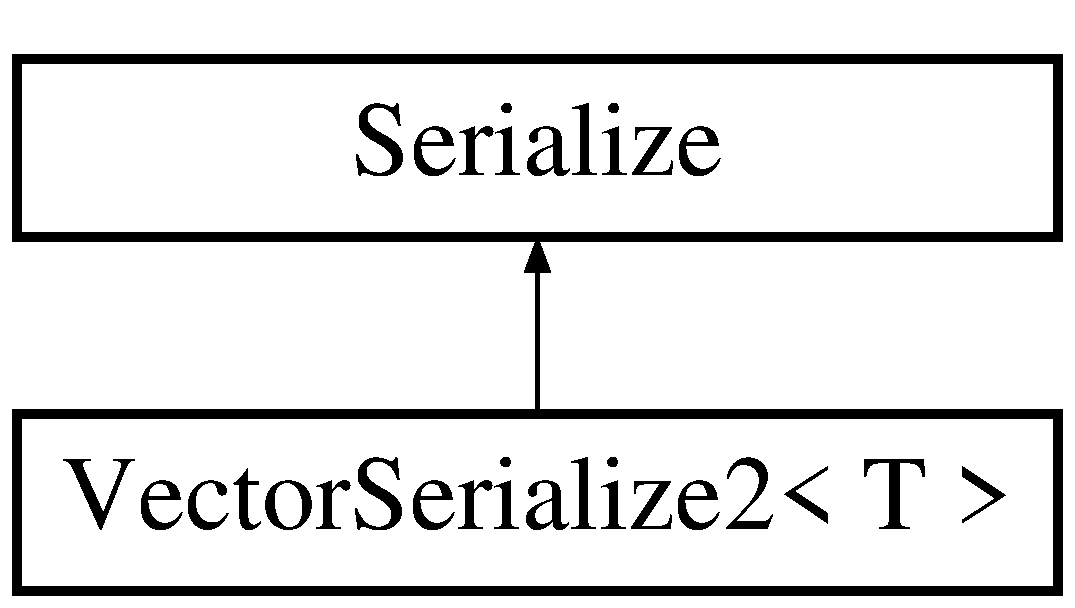
\includegraphics[height=2.000000cm]{classVectorSerialize2}
\end{center}
\end{figure}
\subsection*{Public Member Functions}
\begin{DoxyCompactItemize}
\item 
\hyperlink{classVectorSerialize2_a520cb274e3c0badadd9b95be911ee9a3}{Vector\-Serialize2} (int size, int matiotype)
\item 
\hyperlink{classVectorSerialize2_abf91742790ac898a87b68fd44ed1d70e}{$\sim$\-Vector\-Serialize2} ()
\item 
virtual bool \hyperlink{classVectorSerialize2_a720a62d5c2eb1299d445b35080662aaf}{store} ()
\item 
virtual void \hyperlink{classVectorSerialize2_ae8029b8225cbc4f9e07051949563e473}{clear} ()
\item 
virtual int \hyperlink{classVectorSerialize2_ab73b56a93e5d7ebba81727a16a5f2179}{nstored} ()
\item 
virtual string \hyperlink{classVectorSerialize2_ae0a636c3231b336b7dc8a9b2958b6b0e}{store\-Name} (int indx)
\item 
virtual int \hyperlink{classVectorSerialize2_acc7178f7f25ba6c275041a0e530befdb}{get\-Store\-Class} (int indx)
\item 
virtual void \hyperlink{classVectorSerialize2_a0377d72ce381217f8e8d250509226aec}{get\-Store\-Dims} (int indx, size\-\_\-t $\ast$dims)
\item 
virtual void $\ast$ \hyperlink{classVectorSerialize2_a856c33259537f46fe8c579bd6532a3f4}{get\-Store} (int indx, int k)
\item 
virtual int \hyperlink{classVectorSerialize2_a79c978e6e087c1e7bc398f678d2e943f}{num\-Stores} ()
\item 
virtual double $\ast$ \hyperlink{classVectorSerialize2_a8f4bf0a524b34b584d131b8fbfcd8d30}{mmap\-Read} (double $\ast$d)
\end{DoxyCompactItemize}
\subsection*{Public Attributes}
\begin{DoxyCompactItemize}
\item 
int \hyperlink{classVectorSerialize2_af8eaa31f7a05b4fefedf7c3aea69f89c}{m\-\_\-size}
\item 
int \hyperlink{classVectorSerialize2_a7642e9343ecdbc62835356b89f9c9d2d}{m\-\_\-type}
\item 
double \hyperlink{classVectorSerialize2_ac58f92faa04b0256d02d007846d602b0}{m\-\_\-time}
\item 
vector$<$ T $>$ \hyperlink{classVectorSerialize2_ac7c35c9c34fcc9e1c20fc01704c4c92c}{m\-\_\-stor}
\item 
vector$<$ T $>$ \hyperlink{classVectorSerialize2_a5305cb76c79ff91a0e2a05bb0b76b59c}{m\-\_\-stor2}
\item 
vector$<$ double $>$ \hyperlink{classVectorSerialize2_a22a2c759bc2e39c739ee1010c7f1078c}{v\-\_\-time}
\item 
vector$<$ vector$<$ T $>$ $>$ \hyperlink{classVectorSerialize2_a1606b8f8be4a619436a791c23ce0d644}{v\-\_\-stor}
\item 
vector$<$ vector$<$ T $>$ $>$ \hyperlink{classVectorSerialize2_a9e681c82d96515f9adfce7cc7d6bf2cc}{v\-\_\-stor2}
\item 
T $\ast$ \hyperlink{classVectorSerialize2_aa0db99cb2a6c40c5d7338c7ca250bc00}{m\-\_\-bs}
\end{DoxyCompactItemize}


\subsection{Constructor \& Destructor Documentation}
\hypertarget{classVectorSerialize2_a520cb274e3c0badadd9b95be911ee9a3}{\index{Vector\-Serialize2@{Vector\-Serialize2}!Vector\-Serialize2@{Vector\-Serialize2}}
\index{Vector\-Serialize2@{Vector\-Serialize2}!VectorSerialize2@{Vector\-Serialize2}}
\subsubsection[{Vector\-Serialize2}]{\setlength{\rightskip}{0pt plus 5cm}template$<$class T $>$ {\bf Vector\-Serialize2}$<$ T $>$\-::{\bf Vector\-Serialize2} (
\begin{DoxyParamCaption}
\item[{int}]{size, }
\item[{int}]{matiotype}
\end{DoxyParamCaption}
)}}\label{classVectorSerialize2_a520cb274e3c0badadd9b95be911ee9a3}
\hypertarget{classVectorSerialize2_abf91742790ac898a87b68fd44ed1d70e}{\index{Vector\-Serialize2@{Vector\-Serialize2}!$\sim$\-Vector\-Serialize2@{$\sim$\-Vector\-Serialize2}}
\index{$\sim$\-Vector\-Serialize2@{$\sim$\-Vector\-Serialize2}!VectorSerialize2@{Vector\-Serialize2}}
\subsubsection[{$\sim$\-Vector\-Serialize2}]{\setlength{\rightskip}{0pt plus 5cm}template$<$class T $>$ {\bf Vector\-Serialize2}$<$ T $>$\-::$\sim${\bf Vector\-Serialize2} (
\begin{DoxyParamCaption}
{}
\end{DoxyParamCaption}
)}}\label{classVectorSerialize2_abf91742790ac898a87b68fd44ed1d70e}


\subsection{Member Function Documentation}
\hypertarget{classVectorSerialize2_ae8029b8225cbc4f9e07051949563e473}{\index{Vector\-Serialize2@{Vector\-Serialize2}!clear@{clear}}
\index{clear@{clear}!VectorSerialize2@{Vector\-Serialize2}}
\subsubsection[{clear}]{\setlength{\rightskip}{0pt plus 5cm}template$<$class T $>$ void {\bf Vector\-Serialize2}$<$ T $>$\-::clear (
\begin{DoxyParamCaption}
{}
\end{DoxyParamCaption}
)\hspace{0.3cm}{\ttfamily [virtual]}}}\label{classVectorSerialize2_ae8029b8225cbc4f9e07051949563e473}


Reimplemented from \hyperlink{classSerialize_a11cbf006415c08d1891ab42e39a2aa1a}{Serialize}.

\hypertarget{classVectorSerialize2_a856c33259537f46fe8c579bd6532a3f4}{\index{Vector\-Serialize2@{Vector\-Serialize2}!get\-Store@{get\-Store}}
\index{get\-Store@{get\-Store}!VectorSerialize2@{Vector\-Serialize2}}
\subsubsection[{get\-Store}]{\setlength{\rightskip}{0pt plus 5cm}template$<$class T $>$ void $\ast$ {\bf Vector\-Serialize2}$<$ T $>$\-::get\-Store (
\begin{DoxyParamCaption}
\item[{int}]{indx, }
\item[{int}]{k}
\end{DoxyParamCaption}
)\hspace{0.3cm}{\ttfamily [virtual]}}}\label{classVectorSerialize2_a856c33259537f46fe8c579bd6532a3f4}


Reimplemented from \hyperlink{classSerialize_a6e589d263cfdc0eb72e41687c58831f2}{Serialize}.

\hypertarget{classVectorSerialize2_acc7178f7f25ba6c275041a0e530befdb}{\index{Vector\-Serialize2@{Vector\-Serialize2}!get\-Store\-Class@{get\-Store\-Class}}
\index{get\-Store\-Class@{get\-Store\-Class}!VectorSerialize2@{Vector\-Serialize2}}
\subsubsection[{get\-Store\-Class}]{\setlength{\rightskip}{0pt plus 5cm}template$<$class T $>$ int {\bf Vector\-Serialize2}$<$ T $>$\-::get\-Store\-Class (
\begin{DoxyParamCaption}
\item[{int}]{indx}
\end{DoxyParamCaption}
)\hspace{0.3cm}{\ttfamily [virtual]}}}\label{classVectorSerialize2_acc7178f7f25ba6c275041a0e530befdb}


Reimplemented from \hyperlink{classSerialize_a69954cc86d03b75b6b27511aec4aba43}{Serialize}.

\hypertarget{classVectorSerialize2_a0377d72ce381217f8e8d250509226aec}{\index{Vector\-Serialize2@{Vector\-Serialize2}!get\-Store\-Dims@{get\-Store\-Dims}}
\index{get\-Store\-Dims@{get\-Store\-Dims}!VectorSerialize2@{Vector\-Serialize2}}
\subsubsection[{get\-Store\-Dims}]{\setlength{\rightskip}{0pt plus 5cm}template$<$class T $>$ void {\bf Vector\-Serialize2}$<$ T $>$\-::get\-Store\-Dims (
\begin{DoxyParamCaption}
\item[{int}]{indx, }
\item[{size\-\_\-t $\ast$}]{dims}
\end{DoxyParamCaption}
)\hspace{0.3cm}{\ttfamily [virtual]}}}\label{classVectorSerialize2_a0377d72ce381217f8e8d250509226aec}


Reimplemented from \hyperlink{classSerialize_a52034c5c17bc5e7e6c728b4e6c620c05}{Serialize}.

\hypertarget{classVectorSerialize2_a8f4bf0a524b34b584d131b8fbfcd8d30}{\index{Vector\-Serialize2@{Vector\-Serialize2}!mmap\-Read@{mmap\-Read}}
\index{mmap\-Read@{mmap\-Read}!VectorSerialize2@{Vector\-Serialize2}}
\subsubsection[{mmap\-Read}]{\setlength{\rightskip}{0pt plus 5cm}template$<$class T $>$ double $\ast$ {\bf Vector\-Serialize2}$<$ T $>$\-::mmap\-Read (
\begin{DoxyParamCaption}
\item[{double $\ast$}]{d}
\end{DoxyParamCaption}
)\hspace{0.3cm}{\ttfamily [virtual]}}}\label{classVectorSerialize2_a8f4bf0a524b34b584d131b8fbfcd8d30}


Reimplemented from \hyperlink{classSerialize_a28b939242880e565a8906b30acd0f84c}{Serialize}.



Reimplemented in \hyperlink{classPolhemusSerialize_ac52dec8b5067a7f15a34c9e849be9eff}{Polhemus\-Serialize}, and \hyperlink{classOptoSerialize_a35e6ee49e354276af9548a759fa3f3d2}{Opto\-Serialize}.

\hypertarget{classVectorSerialize2_ab73b56a93e5d7ebba81727a16a5f2179}{\index{Vector\-Serialize2@{Vector\-Serialize2}!nstored@{nstored}}
\index{nstored@{nstored}!VectorSerialize2@{Vector\-Serialize2}}
\subsubsection[{nstored}]{\setlength{\rightskip}{0pt plus 5cm}template$<$class T $>$ int {\bf Vector\-Serialize2}$<$ T $>$\-::nstored (
\begin{DoxyParamCaption}
{}
\end{DoxyParamCaption}
)\hspace{0.3cm}{\ttfamily [virtual]}}}\label{classVectorSerialize2_ab73b56a93e5d7ebba81727a16a5f2179}


Reimplemented from \hyperlink{classSerialize_a590b7308112b07581c03ba826ace50b4}{Serialize}.

\hypertarget{classVectorSerialize2_a79c978e6e087c1e7bc398f678d2e943f}{\index{Vector\-Serialize2@{Vector\-Serialize2}!num\-Stores@{num\-Stores}}
\index{num\-Stores@{num\-Stores}!VectorSerialize2@{Vector\-Serialize2}}
\subsubsection[{num\-Stores}]{\setlength{\rightskip}{0pt plus 5cm}template$<$class T $>$ int {\bf Vector\-Serialize2}$<$ T $>$\-::num\-Stores (
\begin{DoxyParamCaption}
{}
\end{DoxyParamCaption}
)\hspace{0.3cm}{\ttfamily [virtual]}}}\label{classVectorSerialize2_a79c978e6e087c1e7bc398f678d2e943f}


Reimplemented from \hyperlink{classSerialize_a71bf2a906fd71477308a942d01490ab3}{Serialize}.

\hypertarget{classVectorSerialize2_a720a62d5c2eb1299d445b35080662aaf}{\index{Vector\-Serialize2@{Vector\-Serialize2}!store@{store}}
\index{store@{store}!VectorSerialize2@{Vector\-Serialize2}}
\subsubsection[{store}]{\setlength{\rightskip}{0pt plus 5cm}template$<$class T $>$ bool {\bf Vector\-Serialize2}$<$ T $>$\-::store (
\begin{DoxyParamCaption}
{}
\end{DoxyParamCaption}
)\hspace{0.3cm}{\ttfamily [virtual]}}}\label{classVectorSerialize2_a720a62d5c2eb1299d445b35080662aaf}


Reimplemented from \hyperlink{classSerialize_a3cda20e84a530870a6115eaaf589f168}{Serialize}.



Reimplemented in \hyperlink{classPolhemusSerialize_a6cc3ac73da741cdeca76762ce991069c}{Polhemus\-Serialize}, and \hyperlink{classOptoSerialize_aef848193a25e0b103e31f8d25035af16}{Opto\-Serialize}.

\hypertarget{classVectorSerialize2_ae0a636c3231b336b7dc8a9b2958b6b0e}{\index{Vector\-Serialize2@{Vector\-Serialize2}!store\-Name@{store\-Name}}
\index{store\-Name@{store\-Name}!VectorSerialize2@{Vector\-Serialize2}}
\subsubsection[{store\-Name}]{\setlength{\rightskip}{0pt plus 5cm}template$<$class T $>$ string {\bf Vector\-Serialize2}$<$ T $>$\-::store\-Name (
\begin{DoxyParamCaption}
\item[{int}]{indx}
\end{DoxyParamCaption}
)\hspace{0.3cm}{\ttfamily [virtual]}}}\label{classVectorSerialize2_ae0a636c3231b336b7dc8a9b2958b6b0e}


Reimplemented from \hyperlink{classSerialize_ac94a76de6c9376e33b4c195d50ff0568}{Serialize}.



Reimplemented in \hyperlink{classPolhemusSerialize_a9f6cdf8427769c6e23ab2afc7cab07ce}{Polhemus\-Serialize}, and \hyperlink{classOptoSerialize_a6a29e96b87575f2906b65be40c38ceb2}{Opto\-Serialize}.



\subsection{Member Data Documentation}
\hypertarget{classVectorSerialize2_aa0db99cb2a6c40c5d7338c7ca250bc00}{\index{Vector\-Serialize2@{Vector\-Serialize2}!m\-\_\-bs@{m\-\_\-bs}}
\index{m\-\_\-bs@{m\-\_\-bs}!VectorSerialize2@{Vector\-Serialize2}}
\subsubsection[{m\-\_\-bs}]{\setlength{\rightskip}{0pt plus 5cm}template$<$class T$>$ T$\ast$ {\bf Vector\-Serialize2}$<$ T $>$\-::m\-\_\-bs}}\label{classVectorSerialize2_aa0db99cb2a6c40c5d7338c7ca250bc00}
\hypertarget{classVectorSerialize2_af8eaa31f7a05b4fefedf7c3aea69f89c}{\index{Vector\-Serialize2@{Vector\-Serialize2}!m\-\_\-size@{m\-\_\-size}}
\index{m\-\_\-size@{m\-\_\-size}!VectorSerialize2@{Vector\-Serialize2}}
\subsubsection[{m\-\_\-size}]{\setlength{\rightskip}{0pt plus 5cm}template$<$class T$>$ int {\bf Vector\-Serialize2}$<$ T $>$\-::m\-\_\-size}}\label{classVectorSerialize2_af8eaa31f7a05b4fefedf7c3aea69f89c}
\hypertarget{classVectorSerialize2_ac7c35c9c34fcc9e1c20fc01704c4c92c}{\index{Vector\-Serialize2@{Vector\-Serialize2}!m\-\_\-stor@{m\-\_\-stor}}
\index{m\-\_\-stor@{m\-\_\-stor}!VectorSerialize2@{Vector\-Serialize2}}
\subsubsection[{m\-\_\-stor}]{\setlength{\rightskip}{0pt plus 5cm}template$<$class T$>$ vector$<$T$>$ {\bf Vector\-Serialize2}$<$ T $>$\-::m\-\_\-stor}}\label{classVectorSerialize2_ac7c35c9c34fcc9e1c20fc01704c4c92c}
\hypertarget{classVectorSerialize2_a5305cb76c79ff91a0e2a05bb0b76b59c}{\index{Vector\-Serialize2@{Vector\-Serialize2}!m\-\_\-stor2@{m\-\_\-stor2}}
\index{m\-\_\-stor2@{m\-\_\-stor2}!VectorSerialize2@{Vector\-Serialize2}}
\subsubsection[{m\-\_\-stor2}]{\setlength{\rightskip}{0pt plus 5cm}template$<$class T$>$ vector$<$T$>$ {\bf Vector\-Serialize2}$<$ T $>$\-::m\-\_\-stor2}}\label{classVectorSerialize2_a5305cb76c79ff91a0e2a05bb0b76b59c}
\hypertarget{classVectorSerialize2_ac58f92faa04b0256d02d007846d602b0}{\index{Vector\-Serialize2@{Vector\-Serialize2}!m\-\_\-time@{m\-\_\-time}}
\index{m\-\_\-time@{m\-\_\-time}!VectorSerialize2@{Vector\-Serialize2}}
\subsubsection[{m\-\_\-time}]{\setlength{\rightskip}{0pt plus 5cm}template$<$class T$>$ double {\bf Vector\-Serialize2}$<$ T $>$\-::m\-\_\-time}}\label{classVectorSerialize2_ac58f92faa04b0256d02d007846d602b0}
\hypertarget{classVectorSerialize2_a7642e9343ecdbc62835356b89f9c9d2d}{\index{Vector\-Serialize2@{Vector\-Serialize2}!m\-\_\-type@{m\-\_\-type}}
\index{m\-\_\-type@{m\-\_\-type}!VectorSerialize2@{Vector\-Serialize2}}
\subsubsection[{m\-\_\-type}]{\setlength{\rightskip}{0pt plus 5cm}template$<$class T$>$ int {\bf Vector\-Serialize2}$<$ T $>$\-::m\-\_\-type}}\label{classVectorSerialize2_a7642e9343ecdbc62835356b89f9c9d2d}
\hypertarget{classVectorSerialize2_a1606b8f8be4a619436a791c23ce0d644}{\index{Vector\-Serialize2@{Vector\-Serialize2}!v\-\_\-stor@{v\-\_\-stor}}
\index{v\-\_\-stor@{v\-\_\-stor}!VectorSerialize2@{Vector\-Serialize2}}
\subsubsection[{v\-\_\-stor}]{\setlength{\rightskip}{0pt plus 5cm}template$<$class T$>$ vector$<$vector$<$T$>$ $>$ {\bf Vector\-Serialize2}$<$ T $>$\-::v\-\_\-stor}}\label{classVectorSerialize2_a1606b8f8be4a619436a791c23ce0d644}
\hypertarget{classVectorSerialize2_a9e681c82d96515f9adfce7cc7d6bf2cc}{\index{Vector\-Serialize2@{Vector\-Serialize2}!v\-\_\-stor2@{v\-\_\-stor2}}
\index{v\-\_\-stor2@{v\-\_\-stor2}!VectorSerialize2@{Vector\-Serialize2}}
\subsubsection[{v\-\_\-stor2}]{\setlength{\rightskip}{0pt plus 5cm}template$<$class T$>$ vector$<$vector$<$T$>$ $>$ {\bf Vector\-Serialize2}$<$ T $>$\-::v\-\_\-stor2}}\label{classVectorSerialize2_a9e681c82d96515f9adfce7cc7d6bf2cc}
\hypertarget{classVectorSerialize2_a22a2c759bc2e39c739ee1010c7f1078c}{\index{Vector\-Serialize2@{Vector\-Serialize2}!v\-\_\-time@{v\-\_\-time}}
\index{v\-\_\-time@{v\-\_\-time}!VectorSerialize2@{Vector\-Serialize2}}
\subsubsection[{v\-\_\-time}]{\setlength{\rightskip}{0pt plus 5cm}template$<$class T$>$ vector$<$double$>$ {\bf Vector\-Serialize2}$<$ T $>$\-::v\-\_\-time}}\label{classVectorSerialize2_a22a2c759bc2e39c739ee1010c7f1078c}


The documentation for this class was generated from the following file\-:\begin{DoxyCompactItemize}
\item 
/home/ruijan/sw/bmi5/bmi5/include/\-Serialize/\hyperlink{vectorSerialize2_8h}{vector\-Serialize2.\-h}\end{DoxyCompactItemize}

\chapter{File Documentation}
\hypertarget{glFont_8h}{\section{/home/ruijan/sw/bmi5/bmi5/include/gl\-Font.h File Reference}
\label{glFont_8h}\index{/home/ruijan/sw/bmi5/bmi5/include/gl\-Font.\-h@{/home/ruijan/sw/bmi5/bmi5/include/gl\-Font.\-h}}
}
\subsection*{Functions}
\begin{DoxyCompactItemize}
\item 
void \hyperlink{glFont_8h_a469e7890ea4fa330a588480da9e855c1}{Build\-Font} (int display)
\item 
void \hyperlink{glFont_8h_a066dc03f8a57205423cbd545a2400f57}{Kill\-Font} (int display)
\item 
void \hyperlink{glFont_8h_a0cbb492f1bd4e49dca82aa61c0823343}{gl\-Print} (const char $\ast$text, int display)
\end{DoxyCompactItemize}


\subsection{Function Documentation}
\hypertarget{glFont_8h_a469e7890ea4fa330a588480da9e855c1}{\index{gl\-Font.\-h@{gl\-Font.\-h}!Build\-Font@{Build\-Font}}
\index{Build\-Font@{Build\-Font}!glFont.h@{gl\-Font.\-h}}
\subsubsection[{Build\-Font}]{\setlength{\rightskip}{0pt plus 5cm}void Build\-Font (
\begin{DoxyParamCaption}
\item[{int}]{display}
\end{DoxyParamCaption}
)}}\label{glFont_8h_a469e7890ea4fa330a588480da9e855c1}
\hypertarget{glFont_8h_a0cbb492f1bd4e49dca82aa61c0823343}{\index{gl\-Font.\-h@{gl\-Font.\-h}!gl\-Print@{gl\-Print}}
\index{gl\-Print@{gl\-Print}!glFont.h@{gl\-Font.\-h}}
\subsubsection[{gl\-Print}]{\setlength{\rightskip}{0pt plus 5cm}void gl\-Print (
\begin{DoxyParamCaption}
\item[{const char $\ast$}]{text, }
\item[{int}]{display}
\end{DoxyParamCaption}
)}}\label{glFont_8h_a0cbb492f1bd4e49dca82aa61c0823343}
\hypertarget{glFont_8h_a066dc03f8a57205423cbd545a2400f57}{\index{gl\-Font.\-h@{gl\-Font.\-h}!Kill\-Font@{Kill\-Font}}
\index{Kill\-Font@{Kill\-Font}!glFont.h@{gl\-Font.\-h}}
\subsubsection[{Kill\-Font}]{\setlength{\rightskip}{0pt plus 5cm}void Kill\-Font (
\begin{DoxyParamCaption}
\item[{int}]{display}
\end{DoxyParamCaption}
)}}\label{glFont_8h_a066dc03f8a57205423cbd545a2400f57}

\hypertarget{glInfo_8h}{\section{/home/ruijan/sw/bmi5/bmi5/include/gl\-Info.h File Reference}
\label{glInfo_8h}\index{/home/ruijan/sw/bmi5/bmi5/include/gl\-Info.\-h@{/home/ruijan/sw/bmi5/bmi5/include/gl\-Info.\-h}}
}
{\ttfamily \#include $<$string$>$}\\*
{\ttfamily \#include $<$vector$>$}\\*
\subsection*{Classes}
\begin{DoxyCompactItemize}
\item 
struct \hyperlink{structglInfo}{gl\-Info}
\end{DoxyCompactItemize}

\hypertarget{gtkglx_8h}{\section{/home/ruijan/sw/bmi5/bmi5/include/gtkglx.h File Reference}
\label{gtkglx_8h}\index{/home/ruijan/sw/bmi5/bmi5/include/gtkglx.\-h@{/home/ruijan/sw/bmi5/bmi5/include/gtkglx.\-h}}
}
\subsection*{Classes}
\begin{DoxyCompactItemize}
\item 
class \hyperlink{classgtkglx}{gtkglx}
\end{DoxyCompactItemize}

\hypertarget{includeSerialize_8h}{\section{/home/ruijan/sw/bmi5/bmi5/include/include\-Serialize.h File Reference}
\label{includeSerialize_8h}\index{/home/ruijan/sw/bmi5/bmi5/include/include\-Serialize.\-h@{/home/ruijan/sw/bmi5/bmi5/include/include\-Serialize.\-h}}
}
{\ttfamily \#include \char`\"{}Serialize/frame\-Serialize.\-h\char`\"{}}\\*
{\ttfamily \#include \char`\"{}Serialize/labjack\-Serialize\-A\-I\-N.\-h\char`\"{}}\\*
{\ttfamily \#include \char`\"{}Serialize/labjack\-Serialize\-D\-O\-U\-T.\-h\char`\"{}}\\*
{\ttfamily \#include \char`\"{}Serialize/matrix44\-Serialize.\-h\char`\"{}}\\*
{\ttfamily \#include \char`\"{}Serialize/mouse\-Serialize.\-h\char`\"{}}\\*
{\ttfamily \#include \char`\"{}Serialize/opto\-Serialize.\-h\char`\"{}}\\*
{\ttfamily \#include \char`\"{}Serialize/polhemus\-Predict.\-h\char`\"{}}\\*
{\ttfamily \#include \char`\"{}Serialize/polhemus\-Serialize.\-h\char`\"{}}\\*
{\ttfamily \#include \char`\"{}Serialize/tdt\-Udp\-Serialize.\-h\char`\"{}}\\*
{\ttfamily \#include \char`\"{}Serialize/time\-Serialize.\-h\char`\"{}}\\*
{\ttfamily \#include \char`\"{}Serialize/tone\-Serialize.\-h\char`\"{}}\\*
{\ttfamily \#include \char`\"{}Serialize/vector\-Serialize.\-h\char`\"{}}\\*
{\ttfamily \#include \char`\"{}Serialize/vector\-Serialize2.\-h\char`\"{}}\\*

\hypertarget{includeShape_8h}{\section{/home/ruijan/sw/bmi5/bmi5/include/include\-Shape.h File Reference}
\label{includeShape_8h}\index{/home/ruijan/sw/bmi5/bmi5/include/include\-Shape.\-h@{/home/ruijan/sw/bmi5/bmi5/include/include\-Shape.\-h}}
}
{\ttfamily \#include \char`\"{}Shape/ring.\-h\char`\"{}}\\*
{\ttfamily \#include \char`\"{}Shape/circle.\-h\char`\"{}}\\*
{\ttfamily \#include \char`\"{}Shape/line.\-h\char`\"{}}\\*
{\ttfamily \#include \char`\"{}Shape/star\-Field.\-h\char`\"{}}\\*
{\ttfamily \#include \char`\"{}Shape/star\-Field\-Circle.\-h\char`\"{}}\\*
{\ttfamily \#include \char`\"{}Shape/square.\-h\char`\"{}}\\*
{\ttfamily \#include \char`\"{}Shape/open\-Square.\-h\char`\"{}}\\*
{\ttfamily \#include \char`\"{}Shape/display\-Text.\-h\char`\"{}}\\*

\hypertarget{labjackusb_8h}{\section{/home/ruijan/sw/bmi5/bmi5/include/labjackusb.h File Reference}
\label{labjackusb_8h}\index{/home/ruijan/sw/bmi5/bmi5/include/labjackusb.\-h@{/home/ruijan/sw/bmi5/bmi5/include/labjackusb.\-h}}
}
{\ttfamily \#include $<$stdbool.\-h$>$}\\*
\subsection*{Macros}
\begin{DoxyCompactItemize}
\item 
\#define \hyperlink{labjackusb_8h_a751e55770d5889e9f3736c1eedc70d1c}{L\-J\-U\-S\-B\-\_\-\-L\-I\-N\-U\-X\-\_\-\-L\-I\-B\-R\-A\-R\-Y\-\_\-\-V\-E\-R\-S\-I\-O\-N}~2.\-0f
\item 
\#define \hyperlink{labjackusb_8h_ad3deea47eb75da79fb9990e1b0e61f55}{U\-E9\-\_\-\-P\-R\-O\-D\-U\-C\-T\-\_\-\-I\-D}~9
\item 
\#define \hyperlink{labjackusb_8h_ae9f9226ad145f8ad3305f7d5bb0946b7}{U3\-\_\-\-P\-R\-O\-D\-U\-C\-T\-\_\-\-I\-D}~3
\item 
\#define \hyperlink{labjackusb_8h_af648b829b96f509b1f9a904ccfc4c618}{U6\-\_\-\-P\-R\-O\-D\-U\-C\-T\-\_\-\-I\-D}~6
\item 
\#define \hyperlink{labjackusb_8h_a3a4b82e9eb7896ec56d09a56879f1b25}{U12\-\_\-\-P\-R\-O\-D\-U\-C\-T\-\_\-\-I\-D}~1
\item 
\#define \hyperlink{labjackusb_8h_a2fdaca6f1c2ff55d1df17338e1c1a7d1}{B\-R\-I\-D\-G\-E\-\_\-\-P\-R\-O\-D\-U\-C\-T\-\_\-\-I\-D}~0x0501
\item 
\#define \hyperlink{labjackusb_8h_ab5a703b7813b99eb84db2d3e0c47c993}{U\-N\-U\-S\-E\-D\-\_\-\-P\-R\-O\-D\-U\-C\-T\-\_\-\-I\-D}~-\/1
\item 
\#define \hyperlink{labjackusb_8h_a95b5c5d98e6c52d9c3759060983ae2ad}{U\-E9\-\_\-\-P\-I\-P\-E\-\_\-\-E\-P1\-\_\-\-O\-U\-T}~1
\item 
\#define \hyperlink{labjackusb_8h_a41727903fcb0f37140fc33b7594a474e}{U\-E9\-\_\-\-P\-I\-P\-E\-\_\-\-E\-P1\-\_\-\-I\-N}~0x81
\item 
\#define \hyperlink{labjackusb_8h_a22e57e9734bd4f197053a8cbc128306f}{U\-E9\-\_\-\-P\-I\-P\-E\-\_\-\-E\-P2\-\_\-\-I\-N}~0x82
\item 
\#define \hyperlink{labjackusb_8h_a40570367483a9a5da20c3298e04ec419}{U3\-\_\-\-P\-I\-P\-E\-\_\-\-E\-P1\-\_\-\-O\-U\-T}~1
\item 
\#define \hyperlink{labjackusb_8h_ad098f59cf3c61984db9cdddefbefcf93}{U3\-\_\-\-P\-I\-P\-E\-\_\-\-E\-P2\-\_\-\-I\-N}~0x82
\item 
\#define \hyperlink{labjackusb_8h_abdceff9294e5aadf33dcdb82902491a7}{U3\-\_\-\-P\-I\-P\-E\-\_\-\-E\-P3\-\_\-\-I\-N}~0x83
\item 
\#define \hyperlink{labjackusb_8h_a40d7aa8c9f0d46b9c6a10388d7ccdcdc}{U6\-\_\-\-P\-I\-P\-E\-\_\-\-E\-P1\-\_\-\-O\-U\-T}~1
\item 
\#define \hyperlink{labjackusb_8h_a67738d2b6a65bb73176517efd7eda63a}{U6\-\_\-\-P\-I\-P\-E\-\_\-\-E\-P2\-\_\-\-I\-N}~0x82
\item 
\#define \hyperlink{labjackusb_8h_af106ab60345291cc3ced76be0d13b772}{U6\-\_\-\-P\-I\-P\-E\-\_\-\-E\-P3\-\_\-\-I\-N}~0x83
\item 
\#define \hyperlink{labjackusb_8h_a5ebf9682af631e0e13d39142756bbf96}{U12\-\_\-\-P\-I\-P\-E\-\_\-\-E\-P1\-\_\-\-I\-N}~0x81
\item 
\#define \hyperlink{labjackusb_8h_a6d8f18fc14078743be2219b5d29ef9fd}{U12\-\_\-\-P\-I\-P\-E\-\_\-\-E\-P2\-\_\-\-O\-U\-T}~2
\item 
\#define \hyperlink{labjackusb_8h_ad11930a6c6c0f342561d0be1ec42d7c0}{B\-R\-I\-D\-G\-E\-\_\-\-P\-I\-P\-E\-\_\-\-E\-P1\-\_\-\-I\-N}~0x81
\item 
\#define \hyperlink{labjackusb_8h_a7b3688848e747ecb40fae6f6aec6e515}{B\-R\-I\-D\-G\-E\-\_\-\-P\-I\-P\-E\-\_\-\-E\-P1\-\_\-\-O\-U\-T}~1
\end{DoxyCompactItemize}
\subsection*{Typedefs}
\begin{DoxyCompactItemize}
\item 
typedef void $\ast$ \hyperlink{labjackusb_8h_aa8c0374618b33785ccb02f74bcfebc46}{H\-A\-N\-D\-L\-E}
\item 
typedef unsigned int \hyperlink{labjackusb_8h_a36cb3b01d81ffd844bbbfb54003e06ec}{U\-I\-N\-T}
\item 
typedef unsigned char \hyperlink{labjackusb_8h_a4ae1dab0fb4b072a66584546209e7d58}{B\-Y\-T\-E}
\end{DoxyCompactItemize}
\subsection*{Functions}
\begin{DoxyCompactItemize}
\item 
float \hyperlink{labjackusb_8h_a64855c034690f135bee933fefac19a80}{L\-J\-U\-S\-B\-\_\-\-Get\-Library\-Version} (void)
\item 
unsigned long \hyperlink{labjackusb_8h_a0a6ac688cfa2fc6318d83706f4d5d58e}{L\-J\-U\-S\-B\-\_\-\-Get\-Dev\-Count} (unsigned long Product\-I\-D)
\item 
int \hyperlink{labjackusb_8h_a5eaa8d2487a815b45f63b490e4d36257}{L\-J\-U\-S\-B\-\_\-\-Get\-Dev\-Counts} (\hyperlink{labjackusb_8h_a36cb3b01d81ffd844bbbfb54003e06ec}{U\-I\-N\-T} $\ast$product\-Counts, \hyperlink{labjackusb_8h_a36cb3b01d81ffd844bbbfb54003e06ec}{U\-I\-N\-T} $\ast$product\-Ids, \hyperlink{labjackusb_8h_a36cb3b01d81ffd844bbbfb54003e06ec}{U\-I\-N\-T} n)
\item 
int \hyperlink{labjackusb_8h_a89482c49cff21e9b083b6a4b84948cdc}{L\-J\-U\-S\-B\-\_\-\-Open\-All\-Devices} (\hyperlink{labjackusb_8h_aa8c0374618b33785ccb02f74bcfebc46}{H\-A\-N\-D\-L\-E} $\ast$dev\-Handles, \hyperlink{labjackusb_8h_a36cb3b01d81ffd844bbbfb54003e06ec}{U\-I\-N\-T} $\ast$product\-Ids, \hyperlink{labjackusb_8h_a36cb3b01d81ffd844bbbfb54003e06ec}{U\-I\-N\-T} max\-Devices)
\item 
\hyperlink{labjackusb_8h_aa8c0374618b33785ccb02f74bcfebc46}{H\-A\-N\-D\-L\-E} \hyperlink{labjackusb_8h_a757a4f39a73a6cfae6db4324ca750d4b}{L\-J\-U\-S\-B\-\_\-\-Open\-Device} (\hyperlink{labjackusb_8h_a36cb3b01d81ffd844bbbfb54003e06ec}{U\-I\-N\-T} Dev\-Num, unsigned int dw\-Reserved, unsigned long Product\-I\-D)
\item 
unsigned long \hyperlink{labjackusb_8h_a264f717ed8f2fe152b03551577f8d6f8}{L\-J\-U\-S\-B\-\_\-\-Write} (\hyperlink{labjackusb_8h_aa8c0374618b33785ccb02f74bcfebc46}{H\-A\-N\-D\-L\-E} h\-Device, \hyperlink{labjackusb_8h_a4ae1dab0fb4b072a66584546209e7d58}{B\-Y\-T\-E} $\ast$p\-Buff, unsigned long count)
\item 
unsigned long \hyperlink{labjackusb_8h_aa56de181a9e856aa377f7fbcaaff2631}{L\-J\-U\-S\-B\-\_\-\-Read} (\hyperlink{labjackusb_8h_aa8c0374618b33785ccb02f74bcfebc46}{H\-A\-N\-D\-L\-E} h\-Device, \hyperlink{labjackusb_8h_a4ae1dab0fb4b072a66584546209e7d58}{B\-Y\-T\-E} $\ast$p\-Buff, unsigned long count)
\item 
unsigned long \hyperlink{labjackusb_8h_a8fdd7cb5cc51ac9cde5bf66f62cafa11}{L\-J\-U\-S\-B\-\_\-\-Stream} (\hyperlink{labjackusb_8h_aa8c0374618b33785ccb02f74bcfebc46}{H\-A\-N\-D\-L\-E} h\-Device, \hyperlink{labjackusb_8h_a4ae1dab0fb4b072a66584546209e7d58}{B\-Y\-T\-E} $\ast$p\-Buff, unsigned long count)
\item 
void \hyperlink{labjackusb_8h_aeaf4fa0a6025da6ba119e15a32e87404}{L\-J\-U\-S\-B\-\_\-\-Close\-Device} (\hyperlink{labjackusb_8h_aa8c0374618b33785ccb02f74bcfebc46}{H\-A\-N\-D\-L\-E} h\-Device)
\item 
bool \hyperlink{labjackusb_8h_a10e74697d05f37c9663a4625ed6ef2ea}{L\-J\-U\-S\-B\-\_\-\-Is\-Handle\-Valid} (\hyperlink{labjackusb_8h_aa8c0374618b33785ccb02f74bcfebc46}{H\-A\-N\-D\-L\-E} h\-Device)
\item 
bool \hyperlink{labjackusb_8h_aca7f1dad8eb5b815e6dcb10129f29326}{L\-J\-U\-S\-B\-\_\-\-Abort\-Pipe} (\hyperlink{labjackusb_8h_aa8c0374618b33785ccb02f74bcfebc46}{H\-A\-N\-D\-L\-E} h\-Device, unsigned long Pipe)
\item 
unsigned long \hyperlink{labjackusb_8h_ab789911e6165c23d69d0b3d2eacb5024}{L\-J\-U\-S\-B\-\_\-\-Bulk\-Read} (\hyperlink{labjackusb_8h_aa8c0374618b33785ccb02f74bcfebc46}{H\-A\-N\-D\-L\-E} h\-Device, unsigned char endpoint, \hyperlink{labjackusb_8h_a4ae1dab0fb4b072a66584546209e7d58}{B\-Y\-T\-E} $\ast$p\-Buff, unsigned long count)
\item 
unsigned long \hyperlink{labjackusb_8h_a821c2693ef71352ea7006ea88afb3887}{L\-J\-U\-S\-B\-\_\-\-Bulk\-Write} (\hyperlink{labjackusb_8h_aa8c0374618b33785ccb02f74bcfebc46}{H\-A\-N\-D\-L\-E} h\-Device, unsigned char endpoint, \hyperlink{labjackusb_8h_a4ae1dab0fb4b072a66584546209e7d58}{B\-Y\-T\-E} $\ast$p\-Buff, unsigned long count)
\end{DoxyCompactItemize}


\subsection{Macro Definition Documentation}
\hypertarget{labjackusb_8h_ad11930a6c6c0f342561d0be1ec42d7c0}{\index{labjackusb.\-h@{labjackusb.\-h}!B\-R\-I\-D\-G\-E\-\_\-\-P\-I\-P\-E\-\_\-\-E\-P1\-\_\-\-I\-N@{B\-R\-I\-D\-G\-E\-\_\-\-P\-I\-P\-E\-\_\-\-E\-P1\-\_\-\-I\-N}}
\index{B\-R\-I\-D\-G\-E\-\_\-\-P\-I\-P\-E\-\_\-\-E\-P1\-\_\-\-I\-N@{B\-R\-I\-D\-G\-E\-\_\-\-P\-I\-P\-E\-\_\-\-E\-P1\-\_\-\-I\-N}!labjackusb.h@{labjackusb.\-h}}
\subsubsection[{B\-R\-I\-D\-G\-E\-\_\-\-P\-I\-P\-E\-\_\-\-E\-P1\-\_\-\-I\-N}]{\setlength{\rightskip}{0pt plus 5cm}\#define B\-R\-I\-D\-G\-E\-\_\-\-P\-I\-P\-E\-\_\-\-E\-P1\-\_\-\-I\-N~0x81}}\label{labjackusb_8h_ad11930a6c6c0f342561d0be1ec42d7c0}
\hypertarget{labjackusb_8h_a7b3688848e747ecb40fae6f6aec6e515}{\index{labjackusb.\-h@{labjackusb.\-h}!B\-R\-I\-D\-G\-E\-\_\-\-P\-I\-P\-E\-\_\-\-E\-P1\-\_\-\-O\-U\-T@{B\-R\-I\-D\-G\-E\-\_\-\-P\-I\-P\-E\-\_\-\-E\-P1\-\_\-\-O\-U\-T}}
\index{B\-R\-I\-D\-G\-E\-\_\-\-P\-I\-P\-E\-\_\-\-E\-P1\-\_\-\-O\-U\-T@{B\-R\-I\-D\-G\-E\-\_\-\-P\-I\-P\-E\-\_\-\-E\-P1\-\_\-\-O\-U\-T}!labjackusb.h@{labjackusb.\-h}}
\subsubsection[{B\-R\-I\-D\-G\-E\-\_\-\-P\-I\-P\-E\-\_\-\-E\-P1\-\_\-\-O\-U\-T}]{\setlength{\rightskip}{0pt plus 5cm}\#define B\-R\-I\-D\-G\-E\-\_\-\-P\-I\-P\-E\-\_\-\-E\-P1\-\_\-\-O\-U\-T~1}}\label{labjackusb_8h_a7b3688848e747ecb40fae6f6aec6e515}
\hypertarget{labjackusb_8h_a2fdaca6f1c2ff55d1df17338e1c1a7d1}{\index{labjackusb.\-h@{labjackusb.\-h}!B\-R\-I\-D\-G\-E\-\_\-\-P\-R\-O\-D\-U\-C\-T\-\_\-\-I\-D@{B\-R\-I\-D\-G\-E\-\_\-\-P\-R\-O\-D\-U\-C\-T\-\_\-\-I\-D}}
\index{B\-R\-I\-D\-G\-E\-\_\-\-P\-R\-O\-D\-U\-C\-T\-\_\-\-I\-D@{B\-R\-I\-D\-G\-E\-\_\-\-P\-R\-O\-D\-U\-C\-T\-\_\-\-I\-D}!labjackusb.h@{labjackusb.\-h}}
\subsubsection[{B\-R\-I\-D\-G\-E\-\_\-\-P\-R\-O\-D\-U\-C\-T\-\_\-\-I\-D}]{\setlength{\rightskip}{0pt plus 5cm}\#define B\-R\-I\-D\-G\-E\-\_\-\-P\-R\-O\-D\-U\-C\-T\-\_\-\-I\-D~0x0501}}\label{labjackusb_8h_a2fdaca6f1c2ff55d1df17338e1c1a7d1}
\hypertarget{labjackusb_8h_a751e55770d5889e9f3736c1eedc70d1c}{\index{labjackusb.\-h@{labjackusb.\-h}!L\-J\-U\-S\-B\-\_\-\-L\-I\-N\-U\-X\-\_\-\-L\-I\-B\-R\-A\-R\-Y\-\_\-\-V\-E\-R\-S\-I\-O\-N@{L\-J\-U\-S\-B\-\_\-\-L\-I\-N\-U\-X\-\_\-\-L\-I\-B\-R\-A\-R\-Y\-\_\-\-V\-E\-R\-S\-I\-O\-N}}
\index{L\-J\-U\-S\-B\-\_\-\-L\-I\-N\-U\-X\-\_\-\-L\-I\-B\-R\-A\-R\-Y\-\_\-\-V\-E\-R\-S\-I\-O\-N@{L\-J\-U\-S\-B\-\_\-\-L\-I\-N\-U\-X\-\_\-\-L\-I\-B\-R\-A\-R\-Y\-\_\-\-V\-E\-R\-S\-I\-O\-N}!labjackusb.h@{labjackusb.\-h}}
\subsubsection[{L\-J\-U\-S\-B\-\_\-\-L\-I\-N\-U\-X\-\_\-\-L\-I\-B\-R\-A\-R\-Y\-\_\-\-V\-E\-R\-S\-I\-O\-N}]{\setlength{\rightskip}{0pt plus 5cm}\#define L\-J\-U\-S\-B\-\_\-\-L\-I\-N\-U\-X\-\_\-\-L\-I\-B\-R\-A\-R\-Y\-\_\-\-V\-E\-R\-S\-I\-O\-N~2.\-0f}}\label{labjackusb_8h_a751e55770d5889e9f3736c1eedc70d1c}
\hypertarget{labjackusb_8h_a5ebf9682af631e0e13d39142756bbf96}{\index{labjackusb.\-h@{labjackusb.\-h}!U12\-\_\-\-P\-I\-P\-E\-\_\-\-E\-P1\-\_\-\-I\-N@{U12\-\_\-\-P\-I\-P\-E\-\_\-\-E\-P1\-\_\-\-I\-N}}
\index{U12\-\_\-\-P\-I\-P\-E\-\_\-\-E\-P1\-\_\-\-I\-N@{U12\-\_\-\-P\-I\-P\-E\-\_\-\-E\-P1\-\_\-\-I\-N}!labjackusb.h@{labjackusb.\-h}}
\subsubsection[{U12\-\_\-\-P\-I\-P\-E\-\_\-\-E\-P1\-\_\-\-I\-N}]{\setlength{\rightskip}{0pt plus 5cm}\#define U12\-\_\-\-P\-I\-P\-E\-\_\-\-E\-P1\-\_\-\-I\-N~0x81}}\label{labjackusb_8h_a5ebf9682af631e0e13d39142756bbf96}
\hypertarget{labjackusb_8h_a6d8f18fc14078743be2219b5d29ef9fd}{\index{labjackusb.\-h@{labjackusb.\-h}!U12\-\_\-\-P\-I\-P\-E\-\_\-\-E\-P2\-\_\-\-O\-U\-T@{U12\-\_\-\-P\-I\-P\-E\-\_\-\-E\-P2\-\_\-\-O\-U\-T}}
\index{U12\-\_\-\-P\-I\-P\-E\-\_\-\-E\-P2\-\_\-\-O\-U\-T@{U12\-\_\-\-P\-I\-P\-E\-\_\-\-E\-P2\-\_\-\-O\-U\-T}!labjackusb.h@{labjackusb.\-h}}
\subsubsection[{U12\-\_\-\-P\-I\-P\-E\-\_\-\-E\-P2\-\_\-\-O\-U\-T}]{\setlength{\rightskip}{0pt plus 5cm}\#define U12\-\_\-\-P\-I\-P\-E\-\_\-\-E\-P2\-\_\-\-O\-U\-T~2}}\label{labjackusb_8h_a6d8f18fc14078743be2219b5d29ef9fd}
\hypertarget{labjackusb_8h_a3a4b82e9eb7896ec56d09a56879f1b25}{\index{labjackusb.\-h@{labjackusb.\-h}!U12\-\_\-\-P\-R\-O\-D\-U\-C\-T\-\_\-\-I\-D@{U12\-\_\-\-P\-R\-O\-D\-U\-C\-T\-\_\-\-I\-D}}
\index{U12\-\_\-\-P\-R\-O\-D\-U\-C\-T\-\_\-\-I\-D@{U12\-\_\-\-P\-R\-O\-D\-U\-C\-T\-\_\-\-I\-D}!labjackusb.h@{labjackusb.\-h}}
\subsubsection[{U12\-\_\-\-P\-R\-O\-D\-U\-C\-T\-\_\-\-I\-D}]{\setlength{\rightskip}{0pt plus 5cm}\#define U12\-\_\-\-P\-R\-O\-D\-U\-C\-T\-\_\-\-I\-D~1}}\label{labjackusb_8h_a3a4b82e9eb7896ec56d09a56879f1b25}
\hypertarget{labjackusb_8h_a40570367483a9a5da20c3298e04ec419}{\index{labjackusb.\-h@{labjackusb.\-h}!U3\-\_\-\-P\-I\-P\-E\-\_\-\-E\-P1\-\_\-\-O\-U\-T@{U3\-\_\-\-P\-I\-P\-E\-\_\-\-E\-P1\-\_\-\-O\-U\-T}}
\index{U3\-\_\-\-P\-I\-P\-E\-\_\-\-E\-P1\-\_\-\-O\-U\-T@{U3\-\_\-\-P\-I\-P\-E\-\_\-\-E\-P1\-\_\-\-O\-U\-T}!labjackusb.h@{labjackusb.\-h}}
\subsubsection[{U3\-\_\-\-P\-I\-P\-E\-\_\-\-E\-P1\-\_\-\-O\-U\-T}]{\setlength{\rightskip}{0pt plus 5cm}\#define U3\-\_\-\-P\-I\-P\-E\-\_\-\-E\-P1\-\_\-\-O\-U\-T~1}}\label{labjackusb_8h_a40570367483a9a5da20c3298e04ec419}
\hypertarget{labjackusb_8h_ad098f59cf3c61984db9cdddefbefcf93}{\index{labjackusb.\-h@{labjackusb.\-h}!U3\-\_\-\-P\-I\-P\-E\-\_\-\-E\-P2\-\_\-\-I\-N@{U3\-\_\-\-P\-I\-P\-E\-\_\-\-E\-P2\-\_\-\-I\-N}}
\index{U3\-\_\-\-P\-I\-P\-E\-\_\-\-E\-P2\-\_\-\-I\-N@{U3\-\_\-\-P\-I\-P\-E\-\_\-\-E\-P2\-\_\-\-I\-N}!labjackusb.h@{labjackusb.\-h}}
\subsubsection[{U3\-\_\-\-P\-I\-P\-E\-\_\-\-E\-P2\-\_\-\-I\-N}]{\setlength{\rightskip}{0pt plus 5cm}\#define U3\-\_\-\-P\-I\-P\-E\-\_\-\-E\-P2\-\_\-\-I\-N~0x82}}\label{labjackusb_8h_ad098f59cf3c61984db9cdddefbefcf93}
\hypertarget{labjackusb_8h_abdceff9294e5aadf33dcdb82902491a7}{\index{labjackusb.\-h@{labjackusb.\-h}!U3\-\_\-\-P\-I\-P\-E\-\_\-\-E\-P3\-\_\-\-I\-N@{U3\-\_\-\-P\-I\-P\-E\-\_\-\-E\-P3\-\_\-\-I\-N}}
\index{U3\-\_\-\-P\-I\-P\-E\-\_\-\-E\-P3\-\_\-\-I\-N@{U3\-\_\-\-P\-I\-P\-E\-\_\-\-E\-P3\-\_\-\-I\-N}!labjackusb.h@{labjackusb.\-h}}
\subsubsection[{U3\-\_\-\-P\-I\-P\-E\-\_\-\-E\-P3\-\_\-\-I\-N}]{\setlength{\rightskip}{0pt plus 5cm}\#define U3\-\_\-\-P\-I\-P\-E\-\_\-\-E\-P3\-\_\-\-I\-N~0x83}}\label{labjackusb_8h_abdceff9294e5aadf33dcdb82902491a7}
\hypertarget{labjackusb_8h_ae9f9226ad145f8ad3305f7d5bb0946b7}{\index{labjackusb.\-h@{labjackusb.\-h}!U3\-\_\-\-P\-R\-O\-D\-U\-C\-T\-\_\-\-I\-D@{U3\-\_\-\-P\-R\-O\-D\-U\-C\-T\-\_\-\-I\-D}}
\index{U3\-\_\-\-P\-R\-O\-D\-U\-C\-T\-\_\-\-I\-D@{U3\-\_\-\-P\-R\-O\-D\-U\-C\-T\-\_\-\-I\-D}!labjackusb.h@{labjackusb.\-h}}
\subsubsection[{U3\-\_\-\-P\-R\-O\-D\-U\-C\-T\-\_\-\-I\-D}]{\setlength{\rightskip}{0pt plus 5cm}\#define U3\-\_\-\-P\-R\-O\-D\-U\-C\-T\-\_\-\-I\-D~3}}\label{labjackusb_8h_ae9f9226ad145f8ad3305f7d5bb0946b7}
\hypertarget{labjackusb_8h_a40d7aa8c9f0d46b9c6a10388d7ccdcdc}{\index{labjackusb.\-h@{labjackusb.\-h}!U6\-\_\-\-P\-I\-P\-E\-\_\-\-E\-P1\-\_\-\-O\-U\-T@{U6\-\_\-\-P\-I\-P\-E\-\_\-\-E\-P1\-\_\-\-O\-U\-T}}
\index{U6\-\_\-\-P\-I\-P\-E\-\_\-\-E\-P1\-\_\-\-O\-U\-T@{U6\-\_\-\-P\-I\-P\-E\-\_\-\-E\-P1\-\_\-\-O\-U\-T}!labjackusb.h@{labjackusb.\-h}}
\subsubsection[{U6\-\_\-\-P\-I\-P\-E\-\_\-\-E\-P1\-\_\-\-O\-U\-T}]{\setlength{\rightskip}{0pt plus 5cm}\#define U6\-\_\-\-P\-I\-P\-E\-\_\-\-E\-P1\-\_\-\-O\-U\-T~1}}\label{labjackusb_8h_a40d7aa8c9f0d46b9c6a10388d7ccdcdc}
\hypertarget{labjackusb_8h_a67738d2b6a65bb73176517efd7eda63a}{\index{labjackusb.\-h@{labjackusb.\-h}!U6\-\_\-\-P\-I\-P\-E\-\_\-\-E\-P2\-\_\-\-I\-N@{U6\-\_\-\-P\-I\-P\-E\-\_\-\-E\-P2\-\_\-\-I\-N}}
\index{U6\-\_\-\-P\-I\-P\-E\-\_\-\-E\-P2\-\_\-\-I\-N@{U6\-\_\-\-P\-I\-P\-E\-\_\-\-E\-P2\-\_\-\-I\-N}!labjackusb.h@{labjackusb.\-h}}
\subsubsection[{U6\-\_\-\-P\-I\-P\-E\-\_\-\-E\-P2\-\_\-\-I\-N}]{\setlength{\rightskip}{0pt plus 5cm}\#define U6\-\_\-\-P\-I\-P\-E\-\_\-\-E\-P2\-\_\-\-I\-N~0x82}}\label{labjackusb_8h_a67738d2b6a65bb73176517efd7eda63a}
\hypertarget{labjackusb_8h_af106ab60345291cc3ced76be0d13b772}{\index{labjackusb.\-h@{labjackusb.\-h}!U6\-\_\-\-P\-I\-P\-E\-\_\-\-E\-P3\-\_\-\-I\-N@{U6\-\_\-\-P\-I\-P\-E\-\_\-\-E\-P3\-\_\-\-I\-N}}
\index{U6\-\_\-\-P\-I\-P\-E\-\_\-\-E\-P3\-\_\-\-I\-N@{U6\-\_\-\-P\-I\-P\-E\-\_\-\-E\-P3\-\_\-\-I\-N}!labjackusb.h@{labjackusb.\-h}}
\subsubsection[{U6\-\_\-\-P\-I\-P\-E\-\_\-\-E\-P3\-\_\-\-I\-N}]{\setlength{\rightskip}{0pt plus 5cm}\#define U6\-\_\-\-P\-I\-P\-E\-\_\-\-E\-P3\-\_\-\-I\-N~0x83}}\label{labjackusb_8h_af106ab60345291cc3ced76be0d13b772}
\hypertarget{labjackusb_8h_af648b829b96f509b1f9a904ccfc4c618}{\index{labjackusb.\-h@{labjackusb.\-h}!U6\-\_\-\-P\-R\-O\-D\-U\-C\-T\-\_\-\-I\-D@{U6\-\_\-\-P\-R\-O\-D\-U\-C\-T\-\_\-\-I\-D}}
\index{U6\-\_\-\-P\-R\-O\-D\-U\-C\-T\-\_\-\-I\-D@{U6\-\_\-\-P\-R\-O\-D\-U\-C\-T\-\_\-\-I\-D}!labjackusb.h@{labjackusb.\-h}}
\subsubsection[{U6\-\_\-\-P\-R\-O\-D\-U\-C\-T\-\_\-\-I\-D}]{\setlength{\rightskip}{0pt plus 5cm}\#define U6\-\_\-\-P\-R\-O\-D\-U\-C\-T\-\_\-\-I\-D~6}}\label{labjackusb_8h_af648b829b96f509b1f9a904ccfc4c618}
\hypertarget{labjackusb_8h_a41727903fcb0f37140fc33b7594a474e}{\index{labjackusb.\-h@{labjackusb.\-h}!U\-E9\-\_\-\-P\-I\-P\-E\-\_\-\-E\-P1\-\_\-\-I\-N@{U\-E9\-\_\-\-P\-I\-P\-E\-\_\-\-E\-P1\-\_\-\-I\-N}}
\index{U\-E9\-\_\-\-P\-I\-P\-E\-\_\-\-E\-P1\-\_\-\-I\-N@{U\-E9\-\_\-\-P\-I\-P\-E\-\_\-\-E\-P1\-\_\-\-I\-N}!labjackusb.h@{labjackusb.\-h}}
\subsubsection[{U\-E9\-\_\-\-P\-I\-P\-E\-\_\-\-E\-P1\-\_\-\-I\-N}]{\setlength{\rightskip}{0pt plus 5cm}\#define U\-E9\-\_\-\-P\-I\-P\-E\-\_\-\-E\-P1\-\_\-\-I\-N~0x81}}\label{labjackusb_8h_a41727903fcb0f37140fc33b7594a474e}
\hypertarget{labjackusb_8h_a95b5c5d98e6c52d9c3759060983ae2ad}{\index{labjackusb.\-h@{labjackusb.\-h}!U\-E9\-\_\-\-P\-I\-P\-E\-\_\-\-E\-P1\-\_\-\-O\-U\-T@{U\-E9\-\_\-\-P\-I\-P\-E\-\_\-\-E\-P1\-\_\-\-O\-U\-T}}
\index{U\-E9\-\_\-\-P\-I\-P\-E\-\_\-\-E\-P1\-\_\-\-O\-U\-T@{U\-E9\-\_\-\-P\-I\-P\-E\-\_\-\-E\-P1\-\_\-\-O\-U\-T}!labjackusb.h@{labjackusb.\-h}}
\subsubsection[{U\-E9\-\_\-\-P\-I\-P\-E\-\_\-\-E\-P1\-\_\-\-O\-U\-T}]{\setlength{\rightskip}{0pt plus 5cm}\#define U\-E9\-\_\-\-P\-I\-P\-E\-\_\-\-E\-P1\-\_\-\-O\-U\-T~1}}\label{labjackusb_8h_a95b5c5d98e6c52d9c3759060983ae2ad}
\hypertarget{labjackusb_8h_a22e57e9734bd4f197053a8cbc128306f}{\index{labjackusb.\-h@{labjackusb.\-h}!U\-E9\-\_\-\-P\-I\-P\-E\-\_\-\-E\-P2\-\_\-\-I\-N@{U\-E9\-\_\-\-P\-I\-P\-E\-\_\-\-E\-P2\-\_\-\-I\-N}}
\index{U\-E9\-\_\-\-P\-I\-P\-E\-\_\-\-E\-P2\-\_\-\-I\-N@{U\-E9\-\_\-\-P\-I\-P\-E\-\_\-\-E\-P2\-\_\-\-I\-N}!labjackusb.h@{labjackusb.\-h}}
\subsubsection[{U\-E9\-\_\-\-P\-I\-P\-E\-\_\-\-E\-P2\-\_\-\-I\-N}]{\setlength{\rightskip}{0pt plus 5cm}\#define U\-E9\-\_\-\-P\-I\-P\-E\-\_\-\-E\-P2\-\_\-\-I\-N~0x82}}\label{labjackusb_8h_a22e57e9734bd4f197053a8cbc128306f}
\hypertarget{labjackusb_8h_ad3deea47eb75da79fb9990e1b0e61f55}{\index{labjackusb.\-h@{labjackusb.\-h}!U\-E9\-\_\-\-P\-R\-O\-D\-U\-C\-T\-\_\-\-I\-D@{U\-E9\-\_\-\-P\-R\-O\-D\-U\-C\-T\-\_\-\-I\-D}}
\index{U\-E9\-\_\-\-P\-R\-O\-D\-U\-C\-T\-\_\-\-I\-D@{U\-E9\-\_\-\-P\-R\-O\-D\-U\-C\-T\-\_\-\-I\-D}!labjackusb.h@{labjackusb.\-h}}
\subsubsection[{U\-E9\-\_\-\-P\-R\-O\-D\-U\-C\-T\-\_\-\-I\-D}]{\setlength{\rightskip}{0pt plus 5cm}\#define U\-E9\-\_\-\-P\-R\-O\-D\-U\-C\-T\-\_\-\-I\-D~9}}\label{labjackusb_8h_ad3deea47eb75da79fb9990e1b0e61f55}
\hypertarget{labjackusb_8h_ab5a703b7813b99eb84db2d3e0c47c993}{\index{labjackusb.\-h@{labjackusb.\-h}!U\-N\-U\-S\-E\-D\-\_\-\-P\-R\-O\-D\-U\-C\-T\-\_\-\-I\-D@{U\-N\-U\-S\-E\-D\-\_\-\-P\-R\-O\-D\-U\-C\-T\-\_\-\-I\-D}}
\index{U\-N\-U\-S\-E\-D\-\_\-\-P\-R\-O\-D\-U\-C\-T\-\_\-\-I\-D@{U\-N\-U\-S\-E\-D\-\_\-\-P\-R\-O\-D\-U\-C\-T\-\_\-\-I\-D}!labjackusb.h@{labjackusb.\-h}}
\subsubsection[{U\-N\-U\-S\-E\-D\-\_\-\-P\-R\-O\-D\-U\-C\-T\-\_\-\-I\-D}]{\setlength{\rightskip}{0pt plus 5cm}\#define U\-N\-U\-S\-E\-D\-\_\-\-P\-R\-O\-D\-U\-C\-T\-\_\-\-I\-D~-\/1}}\label{labjackusb_8h_ab5a703b7813b99eb84db2d3e0c47c993}


\subsection{Typedef Documentation}
\hypertarget{labjackusb_8h_a4ae1dab0fb4b072a66584546209e7d58}{\index{labjackusb.\-h@{labjackusb.\-h}!B\-Y\-T\-E@{B\-Y\-T\-E}}
\index{B\-Y\-T\-E@{B\-Y\-T\-E}!labjackusb.h@{labjackusb.\-h}}
\subsubsection[{B\-Y\-T\-E}]{\setlength{\rightskip}{0pt plus 5cm}typedef unsigned char {\bf B\-Y\-T\-E}}}\label{labjackusb_8h_a4ae1dab0fb4b072a66584546209e7d58}
\hypertarget{labjackusb_8h_aa8c0374618b33785ccb02f74bcfebc46}{\index{labjackusb.\-h@{labjackusb.\-h}!H\-A\-N\-D\-L\-E@{H\-A\-N\-D\-L\-E}}
\index{H\-A\-N\-D\-L\-E@{H\-A\-N\-D\-L\-E}!labjackusb.h@{labjackusb.\-h}}
\subsubsection[{H\-A\-N\-D\-L\-E}]{\setlength{\rightskip}{0pt plus 5cm}typedef void$\ast$ {\bf H\-A\-N\-D\-L\-E}}}\label{labjackusb_8h_aa8c0374618b33785ccb02f74bcfebc46}
\hypertarget{labjackusb_8h_a36cb3b01d81ffd844bbbfb54003e06ec}{\index{labjackusb.\-h@{labjackusb.\-h}!U\-I\-N\-T@{U\-I\-N\-T}}
\index{U\-I\-N\-T@{U\-I\-N\-T}!labjackusb.h@{labjackusb.\-h}}
\subsubsection[{U\-I\-N\-T}]{\setlength{\rightskip}{0pt plus 5cm}typedef unsigned int {\bf U\-I\-N\-T}}}\label{labjackusb_8h_a36cb3b01d81ffd844bbbfb54003e06ec}


\subsection{Function Documentation}
\hypertarget{labjackusb_8h_aca7f1dad8eb5b815e6dcb10129f29326}{\index{labjackusb.\-h@{labjackusb.\-h}!L\-J\-U\-S\-B\-\_\-\-Abort\-Pipe@{L\-J\-U\-S\-B\-\_\-\-Abort\-Pipe}}
\index{L\-J\-U\-S\-B\-\_\-\-Abort\-Pipe@{L\-J\-U\-S\-B\-\_\-\-Abort\-Pipe}!labjackusb.h@{labjackusb.\-h}}
\subsubsection[{L\-J\-U\-S\-B\-\_\-\-Abort\-Pipe}]{\setlength{\rightskip}{0pt plus 5cm}bool L\-J\-U\-S\-B\-\_\-\-Abort\-Pipe (
\begin{DoxyParamCaption}
\item[{{\bf H\-A\-N\-D\-L\-E}}]{h\-Device, }
\item[{unsigned long}]{Pipe}
\end{DoxyParamCaption}
)}}\label{labjackusb_8h_aca7f1dad8eb5b815e6dcb10129f29326}
\hypertarget{labjackusb_8h_ab789911e6165c23d69d0b3d2eacb5024}{\index{labjackusb.\-h@{labjackusb.\-h}!L\-J\-U\-S\-B\-\_\-\-Bulk\-Read@{L\-J\-U\-S\-B\-\_\-\-Bulk\-Read}}
\index{L\-J\-U\-S\-B\-\_\-\-Bulk\-Read@{L\-J\-U\-S\-B\-\_\-\-Bulk\-Read}!labjackusb.h@{labjackusb.\-h}}
\subsubsection[{L\-J\-U\-S\-B\-\_\-\-Bulk\-Read}]{\setlength{\rightskip}{0pt plus 5cm}unsigned long L\-J\-U\-S\-B\-\_\-\-Bulk\-Read (
\begin{DoxyParamCaption}
\item[{{\bf H\-A\-N\-D\-L\-E}}]{h\-Device, }
\item[{unsigned char}]{endpoint, }
\item[{{\bf B\-Y\-T\-E} $\ast$}]{p\-Buff, }
\item[{unsigned long}]{count}
\end{DoxyParamCaption}
)}}\label{labjackusb_8h_ab789911e6165c23d69d0b3d2eacb5024}
\hypertarget{labjackusb_8h_a821c2693ef71352ea7006ea88afb3887}{\index{labjackusb.\-h@{labjackusb.\-h}!L\-J\-U\-S\-B\-\_\-\-Bulk\-Write@{L\-J\-U\-S\-B\-\_\-\-Bulk\-Write}}
\index{L\-J\-U\-S\-B\-\_\-\-Bulk\-Write@{L\-J\-U\-S\-B\-\_\-\-Bulk\-Write}!labjackusb.h@{labjackusb.\-h}}
\subsubsection[{L\-J\-U\-S\-B\-\_\-\-Bulk\-Write}]{\setlength{\rightskip}{0pt plus 5cm}unsigned long L\-J\-U\-S\-B\-\_\-\-Bulk\-Write (
\begin{DoxyParamCaption}
\item[{{\bf H\-A\-N\-D\-L\-E}}]{h\-Device, }
\item[{unsigned char}]{endpoint, }
\item[{{\bf B\-Y\-T\-E} $\ast$}]{p\-Buff, }
\item[{unsigned long}]{count}
\end{DoxyParamCaption}
)}}\label{labjackusb_8h_a821c2693ef71352ea7006ea88afb3887}
\hypertarget{labjackusb_8h_aeaf4fa0a6025da6ba119e15a32e87404}{\index{labjackusb.\-h@{labjackusb.\-h}!L\-J\-U\-S\-B\-\_\-\-Close\-Device@{L\-J\-U\-S\-B\-\_\-\-Close\-Device}}
\index{L\-J\-U\-S\-B\-\_\-\-Close\-Device@{L\-J\-U\-S\-B\-\_\-\-Close\-Device}!labjackusb.h@{labjackusb.\-h}}
\subsubsection[{L\-J\-U\-S\-B\-\_\-\-Close\-Device}]{\setlength{\rightskip}{0pt plus 5cm}void L\-J\-U\-S\-B\-\_\-\-Close\-Device (
\begin{DoxyParamCaption}
\item[{{\bf H\-A\-N\-D\-L\-E}}]{h\-Device}
\end{DoxyParamCaption}
)}}\label{labjackusb_8h_aeaf4fa0a6025da6ba119e15a32e87404}
\hypertarget{labjackusb_8h_a0a6ac688cfa2fc6318d83706f4d5d58e}{\index{labjackusb.\-h@{labjackusb.\-h}!L\-J\-U\-S\-B\-\_\-\-Get\-Dev\-Count@{L\-J\-U\-S\-B\-\_\-\-Get\-Dev\-Count}}
\index{L\-J\-U\-S\-B\-\_\-\-Get\-Dev\-Count@{L\-J\-U\-S\-B\-\_\-\-Get\-Dev\-Count}!labjackusb.h@{labjackusb.\-h}}
\subsubsection[{L\-J\-U\-S\-B\-\_\-\-Get\-Dev\-Count}]{\setlength{\rightskip}{0pt plus 5cm}unsigned long L\-J\-U\-S\-B\-\_\-\-Get\-Dev\-Count (
\begin{DoxyParamCaption}
\item[{unsigned long}]{Product\-I\-D}
\end{DoxyParamCaption}
)}}\label{labjackusb_8h_a0a6ac688cfa2fc6318d83706f4d5d58e}
\hypertarget{labjackusb_8h_a5eaa8d2487a815b45f63b490e4d36257}{\index{labjackusb.\-h@{labjackusb.\-h}!L\-J\-U\-S\-B\-\_\-\-Get\-Dev\-Counts@{L\-J\-U\-S\-B\-\_\-\-Get\-Dev\-Counts}}
\index{L\-J\-U\-S\-B\-\_\-\-Get\-Dev\-Counts@{L\-J\-U\-S\-B\-\_\-\-Get\-Dev\-Counts}!labjackusb.h@{labjackusb.\-h}}
\subsubsection[{L\-J\-U\-S\-B\-\_\-\-Get\-Dev\-Counts}]{\setlength{\rightskip}{0pt plus 5cm}int L\-J\-U\-S\-B\-\_\-\-Get\-Dev\-Counts (
\begin{DoxyParamCaption}
\item[{{\bf U\-I\-N\-T} $\ast$}]{product\-Counts, }
\item[{{\bf U\-I\-N\-T} $\ast$}]{product\-Ids, }
\item[{{\bf U\-I\-N\-T}}]{n}
\end{DoxyParamCaption}
)}}\label{labjackusb_8h_a5eaa8d2487a815b45f63b490e4d36257}
\hypertarget{labjackusb_8h_a64855c034690f135bee933fefac19a80}{\index{labjackusb.\-h@{labjackusb.\-h}!L\-J\-U\-S\-B\-\_\-\-Get\-Library\-Version@{L\-J\-U\-S\-B\-\_\-\-Get\-Library\-Version}}
\index{L\-J\-U\-S\-B\-\_\-\-Get\-Library\-Version@{L\-J\-U\-S\-B\-\_\-\-Get\-Library\-Version}!labjackusb.h@{labjackusb.\-h}}
\subsubsection[{L\-J\-U\-S\-B\-\_\-\-Get\-Library\-Version}]{\setlength{\rightskip}{0pt plus 5cm}float L\-J\-U\-S\-B\-\_\-\-Get\-Library\-Version (
\begin{DoxyParamCaption}
\item[{void}]{}
\end{DoxyParamCaption}
)}}\label{labjackusb_8h_a64855c034690f135bee933fefac19a80}
\hypertarget{labjackusb_8h_a10e74697d05f37c9663a4625ed6ef2ea}{\index{labjackusb.\-h@{labjackusb.\-h}!L\-J\-U\-S\-B\-\_\-\-Is\-Handle\-Valid@{L\-J\-U\-S\-B\-\_\-\-Is\-Handle\-Valid}}
\index{L\-J\-U\-S\-B\-\_\-\-Is\-Handle\-Valid@{L\-J\-U\-S\-B\-\_\-\-Is\-Handle\-Valid}!labjackusb.h@{labjackusb.\-h}}
\subsubsection[{L\-J\-U\-S\-B\-\_\-\-Is\-Handle\-Valid}]{\setlength{\rightskip}{0pt plus 5cm}bool L\-J\-U\-S\-B\-\_\-\-Is\-Handle\-Valid (
\begin{DoxyParamCaption}
\item[{{\bf H\-A\-N\-D\-L\-E}}]{h\-Device}
\end{DoxyParamCaption}
)}}\label{labjackusb_8h_a10e74697d05f37c9663a4625ed6ef2ea}
\hypertarget{labjackusb_8h_a89482c49cff21e9b083b6a4b84948cdc}{\index{labjackusb.\-h@{labjackusb.\-h}!L\-J\-U\-S\-B\-\_\-\-Open\-All\-Devices@{L\-J\-U\-S\-B\-\_\-\-Open\-All\-Devices}}
\index{L\-J\-U\-S\-B\-\_\-\-Open\-All\-Devices@{L\-J\-U\-S\-B\-\_\-\-Open\-All\-Devices}!labjackusb.h@{labjackusb.\-h}}
\subsubsection[{L\-J\-U\-S\-B\-\_\-\-Open\-All\-Devices}]{\setlength{\rightskip}{0pt plus 5cm}int L\-J\-U\-S\-B\-\_\-\-Open\-All\-Devices (
\begin{DoxyParamCaption}
\item[{{\bf H\-A\-N\-D\-L\-E} $\ast$}]{dev\-Handles, }
\item[{{\bf U\-I\-N\-T} $\ast$}]{product\-Ids, }
\item[{{\bf U\-I\-N\-T}}]{max\-Devices}
\end{DoxyParamCaption}
)}}\label{labjackusb_8h_a89482c49cff21e9b083b6a4b84948cdc}
\hypertarget{labjackusb_8h_a757a4f39a73a6cfae6db4324ca750d4b}{\index{labjackusb.\-h@{labjackusb.\-h}!L\-J\-U\-S\-B\-\_\-\-Open\-Device@{L\-J\-U\-S\-B\-\_\-\-Open\-Device}}
\index{L\-J\-U\-S\-B\-\_\-\-Open\-Device@{L\-J\-U\-S\-B\-\_\-\-Open\-Device}!labjackusb.h@{labjackusb.\-h}}
\subsubsection[{L\-J\-U\-S\-B\-\_\-\-Open\-Device}]{\setlength{\rightskip}{0pt plus 5cm}{\bf H\-A\-N\-D\-L\-E} L\-J\-U\-S\-B\-\_\-\-Open\-Device (
\begin{DoxyParamCaption}
\item[{{\bf U\-I\-N\-T}}]{Dev\-Num, }
\item[{unsigned int}]{dw\-Reserved, }
\item[{unsigned long}]{Product\-I\-D}
\end{DoxyParamCaption}
)}}\label{labjackusb_8h_a757a4f39a73a6cfae6db4324ca750d4b}
\hypertarget{labjackusb_8h_aa56de181a9e856aa377f7fbcaaff2631}{\index{labjackusb.\-h@{labjackusb.\-h}!L\-J\-U\-S\-B\-\_\-\-Read@{L\-J\-U\-S\-B\-\_\-\-Read}}
\index{L\-J\-U\-S\-B\-\_\-\-Read@{L\-J\-U\-S\-B\-\_\-\-Read}!labjackusb.h@{labjackusb.\-h}}
\subsubsection[{L\-J\-U\-S\-B\-\_\-\-Read}]{\setlength{\rightskip}{0pt plus 5cm}unsigned long L\-J\-U\-S\-B\-\_\-\-Read (
\begin{DoxyParamCaption}
\item[{{\bf H\-A\-N\-D\-L\-E}}]{h\-Device, }
\item[{{\bf B\-Y\-T\-E} $\ast$}]{p\-Buff, }
\item[{unsigned long}]{count}
\end{DoxyParamCaption}
)}}\label{labjackusb_8h_aa56de181a9e856aa377f7fbcaaff2631}
\hypertarget{labjackusb_8h_a8fdd7cb5cc51ac9cde5bf66f62cafa11}{\index{labjackusb.\-h@{labjackusb.\-h}!L\-J\-U\-S\-B\-\_\-\-Stream@{L\-J\-U\-S\-B\-\_\-\-Stream}}
\index{L\-J\-U\-S\-B\-\_\-\-Stream@{L\-J\-U\-S\-B\-\_\-\-Stream}!labjackusb.h@{labjackusb.\-h}}
\subsubsection[{L\-J\-U\-S\-B\-\_\-\-Stream}]{\setlength{\rightskip}{0pt plus 5cm}unsigned long L\-J\-U\-S\-B\-\_\-\-Stream (
\begin{DoxyParamCaption}
\item[{{\bf H\-A\-N\-D\-L\-E}}]{h\-Device, }
\item[{{\bf B\-Y\-T\-E} $\ast$}]{p\-Buff, }
\item[{unsigned long}]{count}
\end{DoxyParamCaption}
)}}\label{labjackusb_8h_a8fdd7cb5cc51ac9cde5bf66f62cafa11}
\hypertarget{labjackusb_8h_a264f717ed8f2fe152b03551577f8d6f8}{\index{labjackusb.\-h@{labjackusb.\-h}!L\-J\-U\-S\-B\-\_\-\-Write@{L\-J\-U\-S\-B\-\_\-\-Write}}
\index{L\-J\-U\-S\-B\-\_\-\-Write@{L\-J\-U\-S\-B\-\_\-\-Write}!labjackusb.h@{labjackusb.\-h}}
\subsubsection[{L\-J\-U\-S\-B\-\_\-\-Write}]{\setlength{\rightskip}{0pt plus 5cm}unsigned long L\-J\-U\-S\-B\-\_\-\-Write (
\begin{DoxyParamCaption}
\item[{{\bf H\-A\-N\-D\-L\-E}}]{h\-Device, }
\item[{{\bf B\-Y\-T\-E} $\ast$}]{p\-Buff, }
\item[{unsigned long}]{count}
\end{DoxyParamCaption}
)}}\label{labjackusb_8h_a264f717ed8f2fe152b03551577f8d6f8}

\hypertarget{polhemus_8h}{\section{/home/ruijan/sw/bmi5/bmi5/include/polhemus.h File Reference}
\label{polhemus_8h}\index{/home/ruijan/sw/bmi5/bmi5/include/polhemus.\-h@{/home/ruijan/sw/bmi5/bmi5/include/polhemus.\-h}}
}
{\ttfamily \#include $<$libusb-\/1.\-0/libusb.\-h$>$}\\*
{\ttfamily \#include $<$termios.\-h$>$}\\*
\subsection*{Classes}
\begin{DoxyCompactItemize}
\item 
class \hyperlink{classpolhemus}{polhemus}
\end{DoxyCompactItemize}
\subsection*{Macros}
\begin{DoxyCompactItemize}
\item 
\#define \hyperlink{polhemus_8h_aec93e83855ac17c3c25c55c37ca186dd}{B\-Y\-T\-E}~\hyperlink{u6_8h_adde6aaee8457bee49c2a92621fe22b79}{uint8}
\end{DoxyCompactItemize}
\subsection*{Enumerations}
\begin{DoxyCompactItemize}
\item 
enum \{ \hyperlink{polhemus_8h_a06fc87d81c62e9abb8790b6e5713c55ba896a6824b11cbf6e529d631733ff02e1}{N\-O\-\_\-\-C\-N\-X} =-\/1, 
\hyperlink{polhemus_8h_a06fc87d81c62e9abb8790b6e5713c55baa01beb26836e3a8763bbe5493e32def3}{U\-S\-B\-\_\-\-C\-N\-X}, 
\hyperlink{polhemus_8h_a06fc87d81c62e9abb8790b6e5713c55ba8cf058ed1c1bac3102f203e3cadf0cd4}{R\-S232\-\_\-\-C\-N\-X}
 \}
\item 
enum \{ \\*
\hyperlink{polhemus_8h_adf764cbdea00d65edcd07bb9953ad2b7a8d0e964c5c6e8a545597ddbff97df817}{T\-R\-K\-R\-\_\-\-L\-I\-B\-\_\-\-H\-S}, 
\hyperlink{polhemus_8h_adf764cbdea00d65edcd07bb9953ad2b7a042fd4338c8b98bb7417c42b900c93ec}{T\-R\-K\-R\-\_\-\-L\-I\-B}, 
\hyperlink{polhemus_8h_adf764cbdea00d65edcd07bb9953ad2b7a24250256586b1503cd8900da17e6b755}{T\-R\-K\-R\-\_\-\-P\-A\-T}, 
\hyperlink{polhemus_8h_adf764cbdea00d65edcd07bb9953ad2b7ae787fc5d3fc8c9eaef0a51a9b0208cfb}{T\-R\-K\-R\-\_\-\-F\-T}, 
\\*
\hyperlink{polhemus_8h_adf764cbdea00d65edcd07bb9953ad2b7ad33cfac29ee935192061fc47dd242d82}{N\-U\-M\-\_\-\-S\-U\-P\-P\-\_\-\-T\-R\-K\-S}
 \}
\end{DoxyCompactItemize}


\subsection{Macro Definition Documentation}
\hypertarget{polhemus_8h_aec93e83855ac17c3c25c55c37ca186dd}{\index{polhemus.\-h@{polhemus.\-h}!B\-Y\-T\-E@{B\-Y\-T\-E}}
\index{B\-Y\-T\-E@{B\-Y\-T\-E}!polhemus.h@{polhemus.\-h}}
\subsubsection[{B\-Y\-T\-E}]{\setlength{\rightskip}{0pt plus 5cm}\#define {\bf B\-Y\-T\-E}~{\bf uint8}}}\label{polhemus_8h_aec93e83855ac17c3c25c55c37ca186dd}


\subsection{Enumeration Type Documentation}
\hypertarget{polhemus_8h_a06fc87d81c62e9abb8790b6e5713c55b}{\subsubsection[{anonymous enum}]{\setlength{\rightskip}{0pt plus 5cm}anonymous enum}}\label{polhemus_8h_a06fc87d81c62e9abb8790b6e5713c55b}
\begin{Desc}
\item[Enumerator]\par
\begin{description}
\index{N\-O\-\_\-\-C\-N\-X@{N\-O\-\_\-\-C\-N\-X}!polhemus.\-h@{polhemus.\-h}}\index{polhemus.\-h@{polhemus.\-h}!N\-O\-\_\-\-C\-N\-X@{N\-O\-\_\-\-C\-N\-X}}\item[{\em 
\hypertarget{polhemus_8h_a06fc87d81c62e9abb8790b6e5713c55ba896a6824b11cbf6e529d631733ff02e1}{N\-O\-\_\-\-C\-N\-X}\label{polhemus_8h_a06fc87d81c62e9abb8790b6e5713c55ba896a6824b11cbf6e529d631733ff02e1}
}]\index{U\-S\-B\-\_\-\-C\-N\-X@{U\-S\-B\-\_\-\-C\-N\-X}!polhemus.\-h@{polhemus.\-h}}\index{polhemus.\-h@{polhemus.\-h}!U\-S\-B\-\_\-\-C\-N\-X@{U\-S\-B\-\_\-\-C\-N\-X}}\item[{\em 
\hypertarget{polhemus_8h_a06fc87d81c62e9abb8790b6e5713c55baa01beb26836e3a8763bbe5493e32def3}{U\-S\-B\-\_\-\-C\-N\-X}\label{polhemus_8h_a06fc87d81c62e9abb8790b6e5713c55baa01beb26836e3a8763bbe5493e32def3}
}]\index{R\-S232\-\_\-\-C\-N\-X@{R\-S232\-\_\-\-C\-N\-X}!polhemus.\-h@{polhemus.\-h}}\index{polhemus.\-h@{polhemus.\-h}!R\-S232\-\_\-\-C\-N\-X@{R\-S232\-\_\-\-C\-N\-X}}\item[{\em 
\hypertarget{polhemus_8h_a06fc87d81c62e9abb8790b6e5713c55ba8cf058ed1c1bac3102f203e3cadf0cd4}{R\-S232\-\_\-\-C\-N\-X}\label{polhemus_8h_a06fc87d81c62e9abb8790b6e5713c55ba8cf058ed1c1bac3102f203e3cadf0cd4}
}]\end{description}
\end{Desc}
\hypertarget{polhemus_8h_adf764cbdea00d65edcd07bb9953ad2b7}{\subsubsection[{anonymous enum}]{\setlength{\rightskip}{0pt plus 5cm}anonymous enum}}\label{polhemus_8h_adf764cbdea00d65edcd07bb9953ad2b7}
\begin{Desc}
\item[Enumerator]\par
\begin{description}
\index{T\-R\-K\-R\-\_\-\-L\-I\-B\-\_\-\-H\-S@{T\-R\-K\-R\-\_\-\-L\-I\-B\-\_\-\-H\-S}!polhemus.\-h@{polhemus.\-h}}\index{polhemus.\-h@{polhemus.\-h}!T\-R\-K\-R\-\_\-\-L\-I\-B\-\_\-\-H\-S@{T\-R\-K\-R\-\_\-\-L\-I\-B\-\_\-\-H\-S}}\item[{\em 
\hypertarget{polhemus_8h_adf764cbdea00d65edcd07bb9953ad2b7a8d0e964c5c6e8a545597ddbff97df817}{T\-R\-K\-R\-\_\-\-L\-I\-B\-\_\-\-H\-S}\label{polhemus_8h_adf764cbdea00d65edcd07bb9953ad2b7a8d0e964c5c6e8a545597ddbff97df817}
}]\index{T\-R\-K\-R\-\_\-\-L\-I\-B@{T\-R\-K\-R\-\_\-\-L\-I\-B}!polhemus.\-h@{polhemus.\-h}}\index{polhemus.\-h@{polhemus.\-h}!T\-R\-K\-R\-\_\-\-L\-I\-B@{T\-R\-K\-R\-\_\-\-L\-I\-B}}\item[{\em 
\hypertarget{polhemus_8h_adf764cbdea00d65edcd07bb9953ad2b7a042fd4338c8b98bb7417c42b900c93ec}{T\-R\-K\-R\-\_\-\-L\-I\-B}\label{polhemus_8h_adf764cbdea00d65edcd07bb9953ad2b7a042fd4338c8b98bb7417c42b900c93ec}
}]\index{T\-R\-K\-R\-\_\-\-P\-A\-T@{T\-R\-K\-R\-\_\-\-P\-A\-T}!polhemus.\-h@{polhemus.\-h}}\index{polhemus.\-h@{polhemus.\-h}!T\-R\-K\-R\-\_\-\-P\-A\-T@{T\-R\-K\-R\-\_\-\-P\-A\-T}}\item[{\em 
\hypertarget{polhemus_8h_adf764cbdea00d65edcd07bb9953ad2b7a24250256586b1503cd8900da17e6b755}{T\-R\-K\-R\-\_\-\-P\-A\-T}\label{polhemus_8h_adf764cbdea00d65edcd07bb9953ad2b7a24250256586b1503cd8900da17e6b755}
}]\index{T\-R\-K\-R\-\_\-\-F\-T@{T\-R\-K\-R\-\_\-\-F\-T}!polhemus.\-h@{polhemus.\-h}}\index{polhemus.\-h@{polhemus.\-h}!T\-R\-K\-R\-\_\-\-F\-T@{T\-R\-K\-R\-\_\-\-F\-T}}\item[{\em 
\hypertarget{polhemus_8h_adf764cbdea00d65edcd07bb9953ad2b7ae787fc5d3fc8c9eaef0a51a9b0208cfb}{T\-R\-K\-R\-\_\-\-F\-T}\label{polhemus_8h_adf764cbdea00d65edcd07bb9953ad2b7ae787fc5d3fc8c9eaef0a51a9b0208cfb}
}]\index{N\-U\-M\-\_\-\-S\-U\-P\-P\-\_\-\-T\-R\-K\-S@{N\-U\-M\-\_\-\-S\-U\-P\-P\-\_\-\-T\-R\-K\-S}!polhemus.\-h@{polhemus.\-h}}\index{polhemus.\-h@{polhemus.\-h}!N\-U\-M\-\_\-\-S\-U\-P\-P\-\_\-\-T\-R\-K\-S@{N\-U\-M\-\_\-\-S\-U\-P\-P\-\_\-\-T\-R\-K\-S}}\item[{\em 
\hypertarget{polhemus_8h_adf764cbdea00d65edcd07bb9953ad2b7ad33cfac29ee935192061fc47dd242d82}{N\-U\-M\-\_\-\-S\-U\-P\-P\-\_\-\-T\-R\-K\-S}\label{polhemus_8h_adf764cbdea00d65edcd07bb9953ad2b7ad33cfac29ee935192061fc47dd242d82}
}]\end{description}
\end{Desc}

\hypertarget{frameSerialize_8h}{\section{/home/ruijan/sw/bmi5/bmi5/include/\-Serialize/frame\-Serialize.h File Reference}
\label{frameSerialize_8h}\index{/home/ruijan/sw/bmi5/bmi5/include/\-Serialize/frame\-Serialize.\-h@{/home/ruijan/sw/bmi5/bmi5/include/\-Serialize/frame\-Serialize.\-h}}
}
{\ttfamily \#include \char`\"{}time\-Serialize.\-h\char`\"{}}\\*
\subsection*{Classes}
\begin{DoxyCompactItemize}
\item 
class \hyperlink{classFrameSerialize}{Frame\-Serialize}
\end{DoxyCompactItemize}

\hypertarget{labjackSerializeAIN_8h}{\section{/home/ruijan/sw/bmi5/bmi5/include/\-Serialize/labjack\-Serialize\-A\-I\-N.h File Reference}
\label{labjackSerializeAIN_8h}\index{/home/ruijan/sw/bmi5/bmi5/include/\-Serialize/labjack\-Serialize\-A\-I\-N.\-h@{/home/ruijan/sw/bmi5/bmi5/include/\-Serialize/labjack\-Serialize\-A\-I\-N.\-h}}
}
{\ttfamily \#include \char`\"{}vector\-Serialize.\-h\char`\"{}}\\*
\subsection*{Classes}
\begin{DoxyCompactItemize}
\item 
class \hyperlink{classLabjackSerializeAIN}{Labjack\-Serialize\-A\-I\-N}
\end{DoxyCompactItemize}

\hypertarget{labjackSerializeDOUT_8h}{\section{/home/ruijan/sw/bmi5/bmi5/include/\-Serialize/labjack\-Serialize\-D\-O\-U\-T.h File Reference}
\label{labjackSerializeDOUT_8h}\index{/home/ruijan/sw/bmi5/bmi5/include/\-Serialize/labjack\-Serialize\-D\-O\-U\-T.\-h@{/home/ruijan/sw/bmi5/bmi5/include/\-Serialize/labjack\-Serialize\-D\-O\-U\-T.\-h}}
}
{\ttfamily \#include \char`\"{}vector\-Serialize.\-h\char`\"{}}\\*
\subsection*{Classes}
\begin{DoxyCompactItemize}
\item 
class \hyperlink{classLabjackSerializeDOUT}{Labjack\-Serialize\-D\-O\-U\-T}
\end{DoxyCompactItemize}

\hypertarget{matrix44Serialize_8h}{\section{/home/ruijan/sw/bmi5/bmi5/include/\-Serialize/matrix44\-Serialize.h File Reference}
\label{matrix44Serialize_8h}\index{/home/ruijan/sw/bmi5/bmi5/include/\-Serialize/matrix44\-Serialize.\-h@{/home/ruijan/sw/bmi5/bmi5/include/\-Serialize/matrix44\-Serialize.\-h}}
}
{\ttfamily \#include \char`\"{}serialize.\-h\char`\"{}}\\*
\subsection*{Classes}
\begin{DoxyCompactItemize}
\item 
class \hyperlink{classMatrix44Serialize}{Matrix44\-Serialize}
\end{DoxyCompactItemize}

\hypertarget{mouseSerialize_8h}{\section{/home/ruijan/sw/bmi5/bmi5/include/\-Serialize/mouse\-Serialize.h File Reference}
\label{mouseSerialize_8h}\index{/home/ruijan/sw/bmi5/bmi5/include/\-Serialize/mouse\-Serialize.\-h@{/home/ruijan/sw/bmi5/bmi5/include/\-Serialize/mouse\-Serialize.\-h}}
}
{\ttfamily \#include \char`\"{}vector\-Serialize.\-h\char`\"{}}\\*
\subsection*{Classes}
\begin{DoxyCompactItemize}
\item 
class \hyperlink{classMouseSerialize}{Mouse\-Serialize}
\end{DoxyCompactItemize}

\hypertarget{optoSerialize_8h}{\section{/home/ruijan/sw/bmi5/bmi5/include/\-Serialize/opto\-Serialize.h File Reference}
\label{optoSerialize_8h}\index{/home/ruijan/sw/bmi5/bmi5/include/\-Serialize/opto\-Serialize.\-h@{/home/ruijan/sw/bmi5/bmi5/include/\-Serialize/opto\-Serialize.\-h}}
}
{\ttfamily \#include \char`\"{}vector\-Serialize2.\-h\char`\"{}}\\*
{\ttfamily \#include \char`\"{}polhemus\-Predict.\-h\char`\"{}}\\*
\subsection*{Classes}
\begin{DoxyCompactItemize}
\item 
class \hyperlink{classOptoSerialize}{Opto\-Serialize}
\end{DoxyCompactItemize}

\hypertarget{polhemusPredict_8h}{\section{/home/ruijan/sw/bmi5/bmi5/include/\-Serialize/polhemus\-Predict.h File Reference}
\label{polhemusPredict_8h}\index{/home/ruijan/sw/bmi5/bmi5/include/\-Serialize/polhemus\-Predict.\-h@{/home/ruijan/sw/bmi5/bmi5/include/\-Serialize/polhemus\-Predict.\-h}}
}
{\ttfamily \#include \char`\"{}serialize.\-h\char`\"{}}\\*
\subsection*{Classes}
\begin{DoxyCompactItemize}
\item 
class \hyperlink{classPolhemusPredict}{Polhemus\-Predict}
\end{DoxyCompactItemize}

\hypertarget{polhemusSerialize_8h}{\section{/home/ruijan/sw/bmi5/bmi5/include/\-Serialize/polhemus\-Serialize.h File Reference}
\label{polhemusSerialize_8h}\index{/home/ruijan/sw/bmi5/bmi5/include/\-Serialize/polhemus\-Serialize.\-h@{/home/ruijan/sw/bmi5/bmi5/include/\-Serialize/polhemus\-Serialize.\-h}}
}
{\ttfamily \#include \char`\"{}vector\-Serialize2.\-h\char`\"{}}\\*
{\ttfamily \#include \char`\"{}polhemus\-Predict.\-h\char`\"{}}\\*
\subsection*{Classes}
\begin{DoxyCompactItemize}
\item 
class \hyperlink{classPolhemusSerialize}{Polhemus\-Serialize}
\end{DoxyCompactItemize}

\hypertarget{serialize_8h}{\section{/home/ruijan/sw/bmi5/bmi5/include/\-Serialize/serialize.h File Reference}
\label{serialize_8h}\index{/home/ruijan/sw/bmi5/bmi5/include/\-Serialize/serialize.\-h@{/home/ruijan/sw/bmi5/bmi5/include/\-Serialize/serialize.\-h}}
}
{\ttfamily \#include $<$string$>$}\\*
{\ttfamily \#include $<$vector$>$}\\*
{\ttfamily \#include $<$array$>$}\\*
{\ttfamily \#include \char`\"{}matio.\-h\char`\"{}}\\*
{\ttfamily \#include $<$gsl/gsl\-\_\-fit.\-h$>$}\\*
{\ttfamily \#include $<$string.\-h$>$}\\*
{\ttfamily \#include \char`\"{}gettime.\-h\char`\"{}}\\*
{\ttfamily \#include \char`\"{}timesync.\-h\char`\"{}}\\*
\subsection*{Classes}
\begin{DoxyCompactItemize}
\item 
class \hyperlink{classSerialize}{Serialize}
\end{DoxyCompactItemize}
\subsection*{Functions}
\begin{DoxyCompactItemize}
\item 
long double \hyperlink{serialize_8h_ae7338dc9853460cf73bbf6b5688e47f4}{gettime} ()
\item 
void \hyperlink{serialize_8h_a885699ea354c63ba0e1230584374c5e2}{write\-Matlab} (vector$<$ \hyperlink{classSerialize}{Serialize} $\ast$ $>$ tosave, char $\ast$filename, bool backup)
\item 
size\-\_\-t \hyperlink{serialize_8h_ada20a7f3486117ec825d8d6e5b23bbc8}{matlab\-File\-Size} (vector$<$ \hyperlink{classSerialize}{Serialize} $\ast$ $>$ tosave)
\item 
size\-\_\-t \hyperlink{serialize_8h_a6a04494c2d873936c0c6af8aa5727bf4}{mmap\-File\-Size} (vector$<$ \hyperlink{classSerialize}{Serialize} $\ast$ $>$ tosave)
\item 
bool \hyperlink{serialize_8h_ad5892570856360cb1c1d049c3f2895e9}{matlab\-Has\-New\-Data} (vector$<$ \hyperlink{classSerialize}{Serialize} $\ast$ $>$ tosave)
\end{DoxyCompactItemize}
\subsection*{Variables}
\begin{DoxyCompactItemize}
\item 
Time\-Sync\-Client $\ast$ \hyperlink{serialize_8h_ae17b3579184c8071a510fad0af2921b4}{g\-\_\-tsc}
\item 
int \hyperlink{serialize_8h_a1141b691b2d9da0e106ed031dce903f5}{g\-\_\-frame}
\item 
float \hyperlink{serialize_8h_a9783d947c3be96401bdf2b73cec9b14a}{g\-\_\-mouse\-Pos} \mbox{[}2\mbox{]}
\end{DoxyCompactItemize}


\subsection{Function Documentation}
\hypertarget{serialize_8h_ae7338dc9853460cf73bbf6b5688e47f4}{\index{serialize.\-h@{serialize.\-h}!gettime@{gettime}}
\index{gettime@{gettime}!serialize.h@{serialize.\-h}}
\subsubsection[{gettime}]{\setlength{\rightskip}{0pt plus 5cm}long double gettime (
\begin{DoxyParamCaption}
{}
\end{DoxyParamCaption}
)}}\label{serialize_8h_ae7338dc9853460cf73bbf6b5688e47f4}
\hypertarget{serialize_8h_ada20a7f3486117ec825d8d6e5b23bbc8}{\index{serialize.\-h@{serialize.\-h}!matlab\-File\-Size@{matlab\-File\-Size}}
\index{matlab\-File\-Size@{matlab\-File\-Size}!serialize.h@{serialize.\-h}}
\subsubsection[{matlab\-File\-Size}]{\setlength{\rightskip}{0pt plus 5cm}size\-\_\-t matlab\-File\-Size (
\begin{DoxyParamCaption}
\item[{vector$<$ {\bf Serialize} $\ast$ $>$}]{tosave}
\end{DoxyParamCaption}
)}}\label{serialize_8h_ada20a7f3486117ec825d8d6e5b23bbc8}
\hypertarget{serialize_8h_ad5892570856360cb1c1d049c3f2895e9}{\index{serialize.\-h@{serialize.\-h}!matlab\-Has\-New\-Data@{matlab\-Has\-New\-Data}}
\index{matlab\-Has\-New\-Data@{matlab\-Has\-New\-Data}!serialize.h@{serialize.\-h}}
\subsubsection[{matlab\-Has\-New\-Data}]{\setlength{\rightskip}{0pt plus 5cm}bool matlab\-Has\-New\-Data (
\begin{DoxyParamCaption}
\item[{vector$<$ {\bf Serialize} $\ast$ $>$}]{tosave}
\end{DoxyParamCaption}
)}}\label{serialize_8h_ad5892570856360cb1c1d049c3f2895e9}
\hypertarget{serialize_8h_a6a04494c2d873936c0c6af8aa5727bf4}{\index{serialize.\-h@{serialize.\-h}!mmap\-File\-Size@{mmap\-File\-Size}}
\index{mmap\-File\-Size@{mmap\-File\-Size}!serialize.h@{serialize.\-h}}
\subsubsection[{mmap\-File\-Size}]{\setlength{\rightskip}{0pt plus 5cm}size\-\_\-t mmap\-File\-Size (
\begin{DoxyParamCaption}
\item[{vector$<$ {\bf Serialize} $\ast$ $>$}]{tosave}
\end{DoxyParamCaption}
)}}\label{serialize_8h_a6a04494c2d873936c0c6af8aa5727bf4}
\hypertarget{serialize_8h_a885699ea354c63ba0e1230584374c5e2}{\index{serialize.\-h@{serialize.\-h}!write\-Matlab@{write\-Matlab}}
\index{write\-Matlab@{write\-Matlab}!serialize.h@{serialize.\-h}}
\subsubsection[{write\-Matlab}]{\setlength{\rightskip}{0pt plus 5cm}void write\-Matlab (
\begin{DoxyParamCaption}
\item[{vector$<$ {\bf Serialize} $\ast$ $>$}]{tosave, }
\item[{char $\ast$}]{filename, }
\item[{bool}]{backup}
\end{DoxyParamCaption}
)}}\label{serialize_8h_a885699ea354c63ba0e1230584374c5e2}


\subsection{Variable Documentation}
\hypertarget{serialize_8h_a1141b691b2d9da0e106ed031dce903f5}{\index{serialize.\-h@{serialize.\-h}!g\-\_\-frame@{g\-\_\-frame}}
\index{g\-\_\-frame@{g\-\_\-frame}!serialize.h@{serialize.\-h}}
\subsubsection[{g\-\_\-frame}]{\setlength{\rightskip}{0pt plus 5cm}int g\-\_\-frame}}\label{serialize_8h_a1141b691b2d9da0e106ed031dce903f5}
\hypertarget{serialize_8h_a9783d947c3be96401bdf2b73cec9b14a}{\index{serialize.\-h@{serialize.\-h}!g\-\_\-mouse\-Pos@{g\-\_\-mouse\-Pos}}
\index{g\-\_\-mouse\-Pos@{g\-\_\-mouse\-Pos}!serialize.h@{serialize.\-h}}
\subsubsection[{g\-\_\-mouse\-Pos}]{\setlength{\rightskip}{0pt plus 5cm}float g\-\_\-mouse\-Pos\mbox{[}2\mbox{]}}}\label{serialize_8h_a9783d947c3be96401bdf2b73cec9b14a}
\hypertarget{serialize_8h_ae17b3579184c8071a510fad0af2921b4}{\index{serialize.\-h@{serialize.\-h}!g\-\_\-tsc@{g\-\_\-tsc}}
\index{g\-\_\-tsc@{g\-\_\-tsc}!serialize.h@{serialize.\-h}}
\subsubsection[{g\-\_\-tsc}]{\setlength{\rightskip}{0pt plus 5cm}Time\-Sync\-Client$\ast$ g\-\_\-tsc}}\label{serialize_8h_ae17b3579184c8071a510fad0af2921b4}

\hypertarget{tdtUdpSerialize_8h}{\section{/home/ruijan/sw/bmi5/bmi5/include/\-Serialize/tdt\-Udp\-Serialize.h File Reference}
\label{tdtUdpSerialize_8h}\index{/home/ruijan/sw/bmi5/bmi5/include/\-Serialize/tdt\-Udp\-Serialize.\-h@{/home/ruijan/sw/bmi5/bmi5/include/\-Serialize/tdt\-Udp\-Serialize.\-h}}
}
{\ttfamily \#include \char`\"{}serialize.\-h\char`\"{}}\\*
\subsection*{Classes}
\begin{DoxyCompactItemize}
\item 
class \hyperlink{classTdtUdpSerialize}{Tdt\-Udp\-Serialize}
\end{DoxyCompactItemize}

\hypertarget{timeSerialize_8h}{\section{/home/ruijan/sw/bmi5/bmi5/include/\-Serialize/time\-Serialize.h File Reference}
\label{timeSerialize_8h}\index{/home/ruijan/sw/bmi5/bmi5/include/\-Serialize/time\-Serialize.\-h@{/home/ruijan/sw/bmi5/bmi5/include/\-Serialize/time\-Serialize.\-h}}
}
{\ttfamily \#include \char`\"{}serialize.\-h\char`\"{}}\\*
\subsection*{Classes}
\begin{DoxyCompactItemize}
\item 
class \hyperlink{classTimeSerialize}{Time\-Serialize}
\end{DoxyCompactItemize}

\hypertarget{toneSerialize_8h}{\section{/home/ruijan/sw/bmi5/bmi5/include/\-Serialize/tone\-Serialize.h File Reference}
\label{toneSerialize_8h}\index{/home/ruijan/sw/bmi5/bmi5/include/\-Serialize/tone\-Serialize.\-h@{/home/ruijan/sw/bmi5/bmi5/include/\-Serialize/tone\-Serialize.\-h}}
}
{\ttfamily \#include \char`\"{}serialize.\-h\char`\"{}}\\*
\subsection*{Classes}
\begin{DoxyCompactItemize}
\item 
class \hyperlink{classToneSerialize}{Tone\-Serialize}
\end{DoxyCompactItemize}

\hypertarget{vectorSerialize_8h}{\section{/home/ruijan/sw/bmi5/bmi5/include/\-Serialize/vector\-Serialize.h File Reference}
\label{vectorSerialize_8h}\index{/home/ruijan/sw/bmi5/bmi5/include/\-Serialize/vector\-Serialize.\-h@{/home/ruijan/sw/bmi5/bmi5/include/\-Serialize/vector\-Serialize.\-h}}
}
{\ttfamily \#include \char`\"{}serialize.\-h\char`\"{}}\\*
\subsection*{Classes}
\begin{DoxyCompactItemize}
\item 
class \hyperlink{classVectorSerialize}{Vector\-Serialize$<$ T $>$}
\end{DoxyCompactItemize}

\hypertarget{vectorSerialize2_8h}{\section{/home/ruijan/sw/bmi5/bmi5/include/\-Serialize/vector\-Serialize2.h File Reference}
\label{vectorSerialize2_8h}\index{/home/ruijan/sw/bmi5/bmi5/include/\-Serialize/vector\-Serialize2.\-h@{/home/ruijan/sw/bmi5/bmi5/include/\-Serialize/vector\-Serialize2.\-h}}
}
{\ttfamily \#include \char`\"{}serialize.\-h\char`\"{}}\\*
\subsection*{Classes}
\begin{DoxyCompactItemize}
\item 
class \hyperlink{classVectorSerialize2}{Vector\-Serialize2$<$ T $>$}
\end{DoxyCompactItemize}

\hypertarget{circle_8h}{\section{/home/ruijan/sw/bmi5/bmi5/include/\-Shape/circle.h File Reference}
\label{circle_8h}\index{/home/ruijan/sw/bmi5/bmi5/include/\-Shape/circle.\-h@{/home/ruijan/sw/bmi5/bmi5/include/\-Shape/circle.\-h}}
}
{\ttfamily \#include \char`\"{}shape.\-h\char`\"{}}\\*
\subsection*{Classes}
\begin{DoxyCompactItemize}
\item 
class \hyperlink{classCircle}{Circle}
\end{DoxyCompactItemize}

\hypertarget{displayText_8h}{\section{/home/ruijan/sw/bmi5/bmi5/include/\-Shape/display\-Text.h File Reference}
\label{displayText_8h}\index{/home/ruijan/sw/bmi5/bmi5/include/\-Shape/display\-Text.\-h@{/home/ruijan/sw/bmi5/bmi5/include/\-Shape/display\-Text.\-h}}
}
{\ttfamily \#include \char`\"{}../\-Serialize/vector\-Serialize.\-h\char`\"{}}\\*
\subsection*{Classes}
\begin{DoxyCompactItemize}
\item 
class \hyperlink{classDisplayText}{Display\-Text}
\end{DoxyCompactItemize}

\hypertarget{line_8h}{\section{/home/ruijan/sw/bmi5/bmi5/include/\-Shape/line.h File Reference}
\label{line_8h}\index{/home/ruijan/sw/bmi5/bmi5/include/\-Shape/line.\-h@{/home/ruijan/sw/bmi5/bmi5/include/\-Shape/line.\-h}}
}
{\ttfamily \#include \char`\"{}shape.\-h\char`\"{}}\\*
\subsection*{Classes}
\begin{DoxyCompactItemize}
\item 
class \hyperlink{classLine}{Line}
\end{DoxyCompactItemize}

\hypertarget{magneticField_8h}{\section{/home/ruijan/sw/bmi5/bmi5/include/\-Shape/magnetic\-Field.h File Reference}
\label{magneticField_8h}\index{/home/ruijan/sw/bmi5/bmi5/include/\-Shape/magnetic\-Field.\-h@{/home/ruijan/sw/bmi5/bmi5/include/\-Shape/magnetic\-Field.\-h}}
}

\hypertarget{openSquare_8h}{\section{/home/ruijan/sw/bmi5/bmi5/include/\-Shape/open\-Square.h File Reference}
\label{openSquare_8h}\index{/home/ruijan/sw/bmi5/bmi5/include/\-Shape/open\-Square.\-h@{/home/ruijan/sw/bmi5/bmi5/include/\-Shape/open\-Square.\-h}}
}
{\ttfamily \#include \char`\"{}square.\-h\char`\"{}}\\*
\subsection*{Classes}
\begin{DoxyCompactItemize}
\item 
class \hyperlink{classOpenSquare}{Open\-Square}
\end{DoxyCompactItemize}

\hypertarget{ring_8h}{\section{/home/ruijan/sw/bmi5/bmi5/include/\-Shape/ring.h File Reference}
\label{ring_8h}\index{/home/ruijan/sw/bmi5/bmi5/include/\-Shape/ring.\-h@{/home/ruijan/sw/bmi5/bmi5/include/\-Shape/ring.\-h}}
}
{\ttfamily \#include \char`\"{}shape.\-h\char`\"{}}\\*
\subsection*{Classes}
\begin{DoxyCompactItemize}
\item 
class \hyperlink{classRing}{Ring}
\end{DoxyCompactItemize}

\hypertarget{shape_8h}{\section{/home/ruijan/sw/bmi5/bmi5/include/\-Shape/shape.h File Reference}
\label{shape_8h}\index{/home/ruijan/sw/bmi5/bmi5/include/\-Shape/shape.\-h@{/home/ruijan/sw/bmi5/bmi5/include/\-Shape/shape.\-h}}
}
{\ttfamily \#include $<$iostream$>$}\\*
{\ttfamily \#include \char`\"{}matio.\-h\char`\"{}}\\*
{\ttfamily \#include $<$G\-L/glew.\-h$>$}\\*
{\ttfamily \#include $<$G\-L/glut.\-h$>$}\\*
{\ttfamily \#include $<$G\-L/gl.\-h$>$}\\*
{\ttfamily \#include $<$G\-L/glu.\-h$>$}\\*
{\ttfamily \#include $<$G\-L/glx.\-h$>$}\\*
{\ttfamily \#include $<$G\-L/glext.\-h$>$}\\*
{\ttfamily \#include $<$fstream$>$}\\*
{\ttfamily \#include \char`\"{}gl\-Info.\-h\char`\"{}}\\*
{\ttfamily \#include \char`\"{}gl\-Font.\-h\char`\"{}}\\*
{\ttfamily \#include \char`\"{}../\-Serialize/serialize.\-h\char`\"{}}\\*
{\ttfamily \#include \char`\"{}../include\-Serialize.\-h\char`\"{}}\\*
\subsection*{Classes}
\begin{DoxyCompactItemize}
\item 
class \hyperlink{classShape}{Shape}
\end{DoxyCompactItemize}
\subsection*{Macros}
\begin{DoxyCompactItemize}
\item 
\#define \hyperlink{shape_8h_a598a3330b3c21701223ee0ca14316eca}{P\-I}~3.\-141592653589793
\end{DoxyCompactItemize}
\subsection*{Variables}
\begin{DoxyCompactItemize}
\item 
\hyperlink{classMatrix44Serialize}{Matrix44\-Serialize} $\ast$ \hyperlink{shape_8h_ad50ab51ad954072a1a4653ff4528ca4d}{g\-\_\-affine44}
\item 
\hyperlink{classMatrix44Serialize}{Matrix44\-Serialize} $\ast$ \hyperlink{shape_8h_adf036ec0b6c47003dedcf47c768e4d07}{g\-\_\-quadratic44}
\item 
string \hyperlink{shape_8h_ad4a3140e31ae07f9b34587dfb48c693a}{g\-\_\-basedirname}
\end{DoxyCompactItemize}


\subsection{Macro Definition Documentation}
\hypertarget{shape_8h_a598a3330b3c21701223ee0ca14316eca}{\index{shape.\-h@{shape.\-h}!P\-I@{P\-I}}
\index{P\-I@{P\-I}!shape.h@{shape.\-h}}
\subsubsection[{P\-I}]{\setlength{\rightskip}{0pt plus 5cm}\#define P\-I~3.\-141592653589793}}\label{shape_8h_a598a3330b3c21701223ee0ca14316eca}


\subsection{Variable Documentation}
\hypertarget{shape_8h_ad50ab51ad954072a1a4653ff4528ca4d}{\index{shape.\-h@{shape.\-h}!g\-\_\-affine44@{g\-\_\-affine44}}
\index{g\-\_\-affine44@{g\-\_\-affine44}!shape.h@{shape.\-h}}
\subsubsection[{g\-\_\-affine44}]{\setlength{\rightskip}{0pt plus 5cm}{\bf Matrix44\-Serialize}$\ast$ g\-\_\-affine44}}\label{shape_8h_ad50ab51ad954072a1a4653ff4528ca4d}
\hypertarget{shape_8h_ad4a3140e31ae07f9b34587dfb48c693a}{\index{shape.\-h@{shape.\-h}!g\-\_\-basedirname@{g\-\_\-basedirname}}
\index{g\-\_\-basedirname@{g\-\_\-basedirname}!shape.h@{shape.\-h}}
\subsubsection[{g\-\_\-basedirname}]{\setlength{\rightskip}{0pt plus 5cm}string g\-\_\-basedirname}}\label{shape_8h_ad4a3140e31ae07f9b34587dfb48c693a}
\hypertarget{shape_8h_adf036ec0b6c47003dedcf47c768e4d07}{\index{shape.\-h@{shape.\-h}!g\-\_\-quadratic44@{g\-\_\-quadratic44}}
\index{g\-\_\-quadratic44@{g\-\_\-quadratic44}!shape.h@{shape.\-h}}
\subsubsection[{g\-\_\-quadratic44}]{\setlength{\rightskip}{0pt plus 5cm}{\bf Matrix44\-Serialize}$\ast$ g\-\_\-quadratic44}}\label{shape_8h_adf036ec0b6c47003dedcf47c768e4d07}

\hypertarget{square_8h}{\section{/home/ruijan/sw/bmi5/bmi5/include/\-Shape/square.h File Reference}
\label{square_8h}\index{/home/ruijan/sw/bmi5/bmi5/include/\-Shape/square.\-h@{/home/ruijan/sw/bmi5/bmi5/include/\-Shape/square.\-h}}
}
{\ttfamily \#include \char`\"{}shape.\-h\char`\"{}}\\*
\subsection*{Classes}
\begin{DoxyCompactItemize}
\item 
class \hyperlink{classSquare}{Square}
\end{DoxyCompactItemize}

\hypertarget{starField_8h}{\section{/home/ruijan/sw/bmi5/bmi5/include/\-Shape/star\-Field.h File Reference}
\label{starField_8h}\index{/home/ruijan/sw/bmi5/bmi5/include/\-Shape/star\-Field.\-h@{/home/ruijan/sw/bmi5/bmi5/include/\-Shape/star\-Field.\-h}}
}
{\ttfamily \#include \char`\"{}shape.\-h\char`\"{}}\\*
\subsection*{Classes}
\begin{DoxyCompactItemize}
\item 
struct \hyperlink{structstarStruct}{star\-Struct}
\item 
class \hyperlink{classStarField}{Star\-Field}
\end{DoxyCompactItemize}

\hypertarget{starFieldCircle_8h}{\section{/home/ruijan/sw/bmi5/bmi5/include/\-Shape/star\-Field\-Circle.h File Reference}
\label{starFieldCircle_8h}\index{/home/ruijan/sw/bmi5/bmi5/include/\-Shape/star\-Field\-Circle.\-h@{/home/ruijan/sw/bmi5/bmi5/include/\-Shape/star\-Field\-Circle.\-h}}
}
{\ttfamily \#include \char`\"{}star\-Field.\-h\char`\"{}}\\*
\subsection*{Classes}
\begin{DoxyCompactItemize}
\item 
class \hyperlink{classStarFieldCircle}{Star\-Field\-Circle}
\end{DoxyCompactItemize}

\hypertarget{tdt__udp_8h}{\section{/home/ruijan/sw/bmi5/bmi5/include/tdt\-\_\-udp.h File Reference}
\label{tdt__udp_8h}\index{/home/ruijan/sw/bmi5/bmi5/include/tdt\-\_\-udp.\-h@{/home/ruijan/sw/bmi5/bmi5/include/tdt\-\_\-udp.\-h}}
}
\subsection*{Macros}
\begin{DoxyCompactItemize}
\item 
\#define \hyperlink{tdt__udp_8h_a6b20d41d6252e9871430c242cb1a56e7}{B\-U\-F\-F\-E\-R\-\_\-\-S\-I\-Z\-E}~(\hyperlink{tdt__udp_8h_a99fb83031ce9923c84392b4e92f956b5a688d2c26f77aabab5113fcf6dab67f1e}{H\-E\-A\-D\-E\-R\-\_\-\-B\-Y\-T\-E\-S} + \hyperlink{tdt__udp_8h_a99fb83031ce9923c84392b4e92f956b5a1bf12a95ca02465c6259eabef94fbce0}{M\-A\-X\-\_\-\-S\-A\-M\-P\-L\-E\-S} $\ast$ 4)
\item 
\#define \hyperlink{tdt__udp_8h_af3a13b9edd11a133ec37d932a9f21a32}{M\-A\-K\-E\-\_\-\-H\-E\-A\-D\-E\-R}(cmd, count)~\{ (char)\hyperlink{tdt__udp_8h_a99fb83031ce9923c84392b4e92f956b5ab380e2f1b7ad968d8c158dd8d46ab87f}{H\-E\-A\-D\-E\-R\-\_\-0}, (char)\hyperlink{tdt__udp_8h_a99fb83031ce9923c84392b4e92f956b5ab361a5d48901d71d9dcb62c27978047c}{H\-E\-A\-D\-E\-R\-\_\-1}, cmd, count \}
\item 
\#define \hyperlink{tdt__udp_8h_a5337af39a1f80298de4228baed040a31}{D\-A\-T\-A\-\_\-\-H\-E\-A\-D\-E\-R}(count)~\hyperlink{tdt__udp_8h_af3a13b9edd11a133ec37d932a9f21a32}{M\-A\-K\-E\-\_\-\-H\-E\-A\-D\-E\-R}(\hyperlink{tdt__udp_8h_a99fb83031ce9923c84392b4e92f956b5a1c0bc91aad5ea8b3c62255516456ea64}{D\-A\-T\-A\-\_\-\-P\-A\-C\-K\-E\-T}, count)
\item 
\#define \hyperlink{tdt__udp_8h_a1a12cf3efc59990517aa75a4a33f01a9}{C\-O\-M\-M\-A\-N\-D\-\_\-\-H\-E\-A\-D\-E\-R}(cmd)~\hyperlink{tdt__udp_8h_af3a13b9edd11a133ec37d932a9f21a32}{M\-A\-K\-E\-\_\-\-H\-E\-A\-D\-E\-R}(cmd, 0)
\end{DoxyCompactItemize}
\subsection*{Typedefs}
\begin{DoxyCompactItemize}
\item 
typedef short \hyperlink{tdt__udp_8h_aa343fa3b3d06292b959ffdd4c4703b06}{int16\-\_\-t}
\item 
typedef int \hyperlink{tdt__udp_8h_a32f2e37ee053cf2ce8ca28d1f74630e5}{int32\-\_\-t}
\item 
typedef unsigned char \hyperlink{tdt__udp_8h_aba7bc1797add20fe3efdf37ced1182c5}{uint8\-\_\-t}
\item 
typedef unsigned short \hyperlink{tdt__udp_8h_a273cf69d639a59973b6019625df33e30}{uint16\-\_\-t}
\item 
typedef unsigned int \hyperlink{tdt__udp_8h_a435d1572bf3f880d55459d9805097f62}{uint32\-\_\-t}
\end{DoxyCompactItemize}
\subsection*{Enumerations}
\begin{DoxyCompactItemize}
\item 
enum \{ \\*
\hyperlink{tdt__udp_8h_a99fb83031ce9923c84392b4e92f956b5a1834f9c0e0b9ea8fd42dc642e9821a99}{P\-R\-O\-T\-O\-C\-O\-L\-\_\-\-V\-E\-R\-S\-I\-O\-N} = 1, 
\hyperlink{tdt__udp_8h_a99fb83031ce9923c84392b4e92f956b5a0e6fcc9eb0baabc69143939504a1daf3}{L\-I\-S\-T\-E\-N\-\_\-\-P\-O\-R\-T} = 22022, 
\hyperlink{tdt__udp_8h_a99fb83031ce9923c84392b4e92f956b5ab380e2f1b7ad968d8c158dd8d46ab87f}{H\-E\-A\-D\-E\-R\-\_\-0} = 0x55, 
\hyperlink{tdt__udp_8h_a99fb83031ce9923c84392b4e92f956b5a6ce7695e57784f59c84393510d476741}{H\-E\-A\-D\-E\-R\-\_\-0\-\_\-\-R\-Z2} = 0x00, 
\\*
\hyperlink{tdt__udp_8h_a99fb83031ce9923c84392b4e92f956b5ab361a5d48901d71d9dcb62c27978047c}{H\-E\-A\-D\-E\-R\-\_\-1} = 0x\-A\-A, 
\hyperlink{tdt__udp_8h_a99fb83031ce9923c84392b4e92f956b5af1b0243198f3acf389e6c40c49b5036a}{H\-E\-A\-D\-E\-R\-\_\-2\-\_\-\-R\-Z2} = 0x00, 
\hyperlink{tdt__udp_8h_a99fb83031ce9923c84392b4e92f956b5a688d2c26f77aabab5113fcf6dab67f1e}{H\-E\-A\-D\-E\-R\-\_\-\-B\-Y\-T\-E\-S} = 4, 
\hyperlink{tdt__udp_8h_a99fb83031ce9923c84392b4e92f956b5ab9c96d5239c0648639a2a5ec985547d9}{C\-O\-M\-M\-A\-N\-D\-\_\-\-O\-F\-F\-S\-E\-T} = 2, 
\\*
\hyperlink{tdt__udp_8h_a99fb83031ce9923c84392b4e92f956b5a396ad4da4bdb994d9daca80d15efc1c8}{C\-O\-U\-N\-T\-\_\-\-O\-F\-F\-S\-E\-T} = 3, 
\hyperlink{tdt__udp_8h_a99fb83031ce9923c84392b4e92f956b5ae81cd8da0c30a1d852eb87d4f16b7899}{D\-A\-T\-A\-\_\-\-O\-F\-F\-S\-E\-T} = 4, 
\hyperlink{tdt__udp_8h_a99fb83031ce9923c84392b4e92f956b5a1c0bc91aad5ea8b3c62255516456ea64}{D\-A\-T\-A\-\_\-\-P\-A\-C\-K\-E\-T} = 0, 
\hyperlink{tdt__udp_8h_a99fb83031ce9923c84392b4e92f956b5a2802e25e9b7a05b5382335bb8185d63c}{G\-E\-T\-\_\-\-V\-E\-R\-S\-I\-O\-N} = 1, 
\\*
\hyperlink{tdt__udp_8h_a99fb83031ce9923c84392b4e92f956b5ae4c4eef937d9318f6aef1d3c454813e5}{S\-E\-T\-\_\-\-R\-E\-M\-O\-T\-E\-\_\-\-I\-P} = 2, 
\hyperlink{tdt__udp_8h_a99fb83031ce9923c84392b4e92f956b5a8660c408f3356a3936a3bcaf0ebad218}{F\-O\-R\-G\-E\-T\-\_\-\-R\-E\-M\-O\-T\-E\-\_\-\-I\-P} = 3, 
\hyperlink{tdt__udp_8h_a99fb83031ce9923c84392b4e92f956b5aa376a8aa0a1b95dab0326b4989a48526}{R\-E\-S\-E\-T\-\_\-\-T\-O\-\_\-\-D\-E\-F\-A\-U\-L\-T\-S} = 0x\-F\-F, 
\hyperlink{tdt__udp_8h_a99fb83031ce9923c84392b4e92f956b5a1bf12a95ca02465c6259eabef94fbce0}{M\-A\-X\-\_\-\-S\-A\-M\-P\-L\-E\-S} = 244
 \}
\end{DoxyCompactItemize}
\subsection*{Functions}
\begin{DoxyCompactItemize}
\item 
int \hyperlink{tdt__udp_8h_a01e6b38441f8188c1ae46622d2ae43bf}{open\-Socket} (char $\ast$str\-I\-P\-Addr, int port)
\item 
bool \hyperlink{tdt__udp_8h_a164e1f33e01633c3e3a1236a244791ba}{check\-R\-Z} (int sock)
\item 
bool \hyperlink{tdt__udp_8h_a8e4e48ce5f02f0e39cc7ad594cc5dcb3}{send\-Data\-R\-Z} (int sock, float $\ast$data, int count)
\item 
void \hyperlink{tdt__udp_8h_a65f9ae58a709b3e82cad120f396a0f6a}{disconnect\-R\-Z} (int sock)
\end{DoxyCompactItemize}


\subsection{Macro Definition Documentation}
\hypertarget{tdt__udp_8h_a6b20d41d6252e9871430c242cb1a56e7}{\index{tdt\-\_\-udp.\-h@{tdt\-\_\-udp.\-h}!B\-U\-F\-F\-E\-R\-\_\-\-S\-I\-Z\-E@{B\-U\-F\-F\-E\-R\-\_\-\-S\-I\-Z\-E}}
\index{B\-U\-F\-F\-E\-R\-\_\-\-S\-I\-Z\-E@{B\-U\-F\-F\-E\-R\-\_\-\-S\-I\-Z\-E}!tdt_udp.h@{tdt\-\_\-udp.\-h}}
\subsubsection[{B\-U\-F\-F\-E\-R\-\_\-\-S\-I\-Z\-E}]{\setlength{\rightskip}{0pt plus 5cm}\#define B\-U\-F\-F\-E\-R\-\_\-\-S\-I\-Z\-E~({\bf H\-E\-A\-D\-E\-R\-\_\-\-B\-Y\-T\-E\-S} + {\bf M\-A\-X\-\_\-\-S\-A\-M\-P\-L\-E\-S} $\ast$ 4)}}\label{tdt__udp_8h_a6b20d41d6252e9871430c242cb1a56e7}
\hypertarget{tdt__udp_8h_a1a12cf3efc59990517aa75a4a33f01a9}{\index{tdt\-\_\-udp.\-h@{tdt\-\_\-udp.\-h}!C\-O\-M\-M\-A\-N\-D\-\_\-\-H\-E\-A\-D\-E\-R@{C\-O\-M\-M\-A\-N\-D\-\_\-\-H\-E\-A\-D\-E\-R}}
\index{C\-O\-M\-M\-A\-N\-D\-\_\-\-H\-E\-A\-D\-E\-R@{C\-O\-M\-M\-A\-N\-D\-\_\-\-H\-E\-A\-D\-E\-R}!tdt_udp.h@{tdt\-\_\-udp.\-h}}
\subsubsection[{C\-O\-M\-M\-A\-N\-D\-\_\-\-H\-E\-A\-D\-E\-R}]{\setlength{\rightskip}{0pt plus 5cm}\#define C\-O\-M\-M\-A\-N\-D\-\_\-\-H\-E\-A\-D\-E\-R(
\begin{DoxyParamCaption}
\item[{}]{cmd}
\end{DoxyParamCaption}
)~{\bf M\-A\-K\-E\-\_\-\-H\-E\-A\-D\-E\-R}(cmd, 0)}}\label{tdt__udp_8h_a1a12cf3efc59990517aa75a4a33f01a9}
\hypertarget{tdt__udp_8h_a5337af39a1f80298de4228baed040a31}{\index{tdt\-\_\-udp.\-h@{tdt\-\_\-udp.\-h}!D\-A\-T\-A\-\_\-\-H\-E\-A\-D\-E\-R@{D\-A\-T\-A\-\_\-\-H\-E\-A\-D\-E\-R}}
\index{D\-A\-T\-A\-\_\-\-H\-E\-A\-D\-E\-R@{D\-A\-T\-A\-\_\-\-H\-E\-A\-D\-E\-R}!tdt_udp.h@{tdt\-\_\-udp.\-h}}
\subsubsection[{D\-A\-T\-A\-\_\-\-H\-E\-A\-D\-E\-R}]{\setlength{\rightskip}{0pt plus 5cm}\#define D\-A\-T\-A\-\_\-\-H\-E\-A\-D\-E\-R(
\begin{DoxyParamCaption}
\item[{}]{count}
\end{DoxyParamCaption}
)~{\bf M\-A\-K\-E\-\_\-\-H\-E\-A\-D\-E\-R}({\bf D\-A\-T\-A\-\_\-\-P\-A\-C\-K\-E\-T}, count)}}\label{tdt__udp_8h_a5337af39a1f80298de4228baed040a31}
\hypertarget{tdt__udp_8h_af3a13b9edd11a133ec37d932a9f21a32}{\index{tdt\-\_\-udp.\-h@{tdt\-\_\-udp.\-h}!M\-A\-K\-E\-\_\-\-H\-E\-A\-D\-E\-R@{M\-A\-K\-E\-\_\-\-H\-E\-A\-D\-E\-R}}
\index{M\-A\-K\-E\-\_\-\-H\-E\-A\-D\-E\-R@{M\-A\-K\-E\-\_\-\-H\-E\-A\-D\-E\-R}!tdt_udp.h@{tdt\-\_\-udp.\-h}}
\subsubsection[{M\-A\-K\-E\-\_\-\-H\-E\-A\-D\-E\-R}]{\setlength{\rightskip}{0pt plus 5cm}\#define M\-A\-K\-E\-\_\-\-H\-E\-A\-D\-E\-R(
\begin{DoxyParamCaption}
\item[{}]{cmd, }
\item[{}]{count}
\end{DoxyParamCaption}
)~\{ (char){\bf H\-E\-A\-D\-E\-R\-\_\-0}, (char){\bf H\-E\-A\-D\-E\-R\-\_\-1}, cmd, count \}}}\label{tdt__udp_8h_af3a13b9edd11a133ec37d932a9f21a32}


\subsection{Typedef Documentation}
\hypertarget{tdt__udp_8h_aa343fa3b3d06292b959ffdd4c4703b06}{\index{tdt\-\_\-udp.\-h@{tdt\-\_\-udp.\-h}!int16\-\_\-t@{int16\-\_\-t}}
\index{int16\-\_\-t@{int16\-\_\-t}!tdt_udp.h@{tdt\-\_\-udp.\-h}}
\subsubsection[{int16\-\_\-t}]{\setlength{\rightskip}{0pt plus 5cm}typedef short {\bf int16\-\_\-t}}}\label{tdt__udp_8h_aa343fa3b3d06292b959ffdd4c4703b06}
\hypertarget{tdt__udp_8h_a32f2e37ee053cf2ce8ca28d1f74630e5}{\index{tdt\-\_\-udp.\-h@{tdt\-\_\-udp.\-h}!int32\-\_\-t@{int32\-\_\-t}}
\index{int32\-\_\-t@{int32\-\_\-t}!tdt_udp.h@{tdt\-\_\-udp.\-h}}
\subsubsection[{int32\-\_\-t}]{\setlength{\rightskip}{0pt plus 5cm}typedef int {\bf int32\-\_\-t}}}\label{tdt__udp_8h_a32f2e37ee053cf2ce8ca28d1f74630e5}
\hypertarget{tdt__udp_8h_a273cf69d639a59973b6019625df33e30}{\index{tdt\-\_\-udp.\-h@{tdt\-\_\-udp.\-h}!uint16\-\_\-t@{uint16\-\_\-t}}
\index{uint16\-\_\-t@{uint16\-\_\-t}!tdt_udp.h@{tdt\-\_\-udp.\-h}}
\subsubsection[{uint16\-\_\-t}]{\setlength{\rightskip}{0pt plus 5cm}typedef unsigned short {\bf uint16\-\_\-t}}}\label{tdt__udp_8h_a273cf69d639a59973b6019625df33e30}
\hypertarget{tdt__udp_8h_a435d1572bf3f880d55459d9805097f62}{\index{tdt\-\_\-udp.\-h@{tdt\-\_\-udp.\-h}!uint32\-\_\-t@{uint32\-\_\-t}}
\index{uint32\-\_\-t@{uint32\-\_\-t}!tdt_udp.h@{tdt\-\_\-udp.\-h}}
\subsubsection[{uint32\-\_\-t}]{\setlength{\rightskip}{0pt plus 5cm}typedef unsigned int {\bf uint32\-\_\-t}}}\label{tdt__udp_8h_a435d1572bf3f880d55459d9805097f62}
\hypertarget{tdt__udp_8h_aba7bc1797add20fe3efdf37ced1182c5}{\index{tdt\-\_\-udp.\-h@{tdt\-\_\-udp.\-h}!uint8\-\_\-t@{uint8\-\_\-t}}
\index{uint8\-\_\-t@{uint8\-\_\-t}!tdt_udp.h@{tdt\-\_\-udp.\-h}}
\subsubsection[{uint8\-\_\-t}]{\setlength{\rightskip}{0pt plus 5cm}typedef unsigned char {\bf uint8\-\_\-t}}}\label{tdt__udp_8h_aba7bc1797add20fe3efdf37ced1182c5}


\subsection{Enumeration Type Documentation}
\hypertarget{tdt__udp_8h_a99fb83031ce9923c84392b4e92f956b5}{\subsubsection[{anonymous enum}]{\setlength{\rightskip}{0pt plus 5cm}anonymous enum}}\label{tdt__udp_8h_a99fb83031ce9923c84392b4e92f956b5}
\begin{Desc}
\item[Enumerator]\par
\begin{description}
\index{P\-R\-O\-T\-O\-C\-O\-L\-\_\-\-V\-E\-R\-S\-I\-O\-N@{P\-R\-O\-T\-O\-C\-O\-L\-\_\-\-V\-E\-R\-S\-I\-O\-N}!tdt\-\_\-udp.\-h@{tdt\-\_\-udp.\-h}}\index{tdt\-\_\-udp.\-h@{tdt\-\_\-udp.\-h}!P\-R\-O\-T\-O\-C\-O\-L\-\_\-\-V\-E\-R\-S\-I\-O\-N@{P\-R\-O\-T\-O\-C\-O\-L\-\_\-\-V\-E\-R\-S\-I\-O\-N}}\item[{\em 
\hypertarget{tdt__udp_8h_a99fb83031ce9923c84392b4e92f956b5a1834f9c0e0b9ea8fd42dc642e9821a99}{P\-R\-O\-T\-O\-C\-O\-L\-\_\-\-V\-E\-R\-S\-I\-O\-N}\label{tdt__udp_8h_a99fb83031ce9923c84392b4e92f956b5a1834f9c0e0b9ea8fd42dc642e9821a99}
}]\index{L\-I\-S\-T\-E\-N\-\_\-\-P\-O\-R\-T@{L\-I\-S\-T\-E\-N\-\_\-\-P\-O\-R\-T}!tdt\-\_\-udp.\-h@{tdt\-\_\-udp.\-h}}\index{tdt\-\_\-udp.\-h@{tdt\-\_\-udp.\-h}!L\-I\-S\-T\-E\-N\-\_\-\-P\-O\-R\-T@{L\-I\-S\-T\-E\-N\-\_\-\-P\-O\-R\-T}}\item[{\em 
\hypertarget{tdt__udp_8h_a99fb83031ce9923c84392b4e92f956b5a0e6fcc9eb0baabc69143939504a1daf3}{L\-I\-S\-T\-E\-N\-\_\-\-P\-O\-R\-T}\label{tdt__udp_8h_a99fb83031ce9923c84392b4e92f956b5a0e6fcc9eb0baabc69143939504a1daf3}
}]\index{H\-E\-A\-D\-E\-R\-\_\-0@{H\-E\-A\-D\-E\-R\-\_\-0}!tdt\-\_\-udp.\-h@{tdt\-\_\-udp.\-h}}\index{tdt\-\_\-udp.\-h@{tdt\-\_\-udp.\-h}!H\-E\-A\-D\-E\-R\-\_\-0@{H\-E\-A\-D\-E\-R\-\_\-0}}\item[{\em 
\hypertarget{tdt__udp_8h_a99fb83031ce9923c84392b4e92f956b5ab380e2f1b7ad968d8c158dd8d46ab87f}{H\-E\-A\-D\-E\-R\-\_\-0}\label{tdt__udp_8h_a99fb83031ce9923c84392b4e92f956b5ab380e2f1b7ad968d8c158dd8d46ab87f}
}]\index{H\-E\-A\-D\-E\-R\-\_\-0\-\_\-\-R\-Z2@{H\-E\-A\-D\-E\-R\-\_\-0\-\_\-\-R\-Z2}!tdt\-\_\-udp.\-h@{tdt\-\_\-udp.\-h}}\index{tdt\-\_\-udp.\-h@{tdt\-\_\-udp.\-h}!H\-E\-A\-D\-E\-R\-\_\-0\-\_\-\-R\-Z2@{H\-E\-A\-D\-E\-R\-\_\-0\-\_\-\-R\-Z2}}\item[{\em 
\hypertarget{tdt__udp_8h_a99fb83031ce9923c84392b4e92f956b5a6ce7695e57784f59c84393510d476741}{H\-E\-A\-D\-E\-R\-\_\-0\-\_\-\-R\-Z2}\label{tdt__udp_8h_a99fb83031ce9923c84392b4e92f956b5a6ce7695e57784f59c84393510d476741}
}]\index{H\-E\-A\-D\-E\-R\-\_\-1@{H\-E\-A\-D\-E\-R\-\_\-1}!tdt\-\_\-udp.\-h@{tdt\-\_\-udp.\-h}}\index{tdt\-\_\-udp.\-h@{tdt\-\_\-udp.\-h}!H\-E\-A\-D\-E\-R\-\_\-1@{H\-E\-A\-D\-E\-R\-\_\-1}}\item[{\em 
\hypertarget{tdt__udp_8h_a99fb83031ce9923c84392b4e92f956b5ab361a5d48901d71d9dcb62c27978047c}{H\-E\-A\-D\-E\-R\-\_\-1}\label{tdt__udp_8h_a99fb83031ce9923c84392b4e92f956b5ab361a5d48901d71d9dcb62c27978047c}
}]\index{H\-E\-A\-D\-E\-R\-\_\-2\-\_\-\-R\-Z2@{H\-E\-A\-D\-E\-R\-\_\-2\-\_\-\-R\-Z2}!tdt\-\_\-udp.\-h@{tdt\-\_\-udp.\-h}}\index{tdt\-\_\-udp.\-h@{tdt\-\_\-udp.\-h}!H\-E\-A\-D\-E\-R\-\_\-2\-\_\-\-R\-Z2@{H\-E\-A\-D\-E\-R\-\_\-2\-\_\-\-R\-Z2}}\item[{\em 
\hypertarget{tdt__udp_8h_a99fb83031ce9923c84392b4e92f956b5af1b0243198f3acf389e6c40c49b5036a}{H\-E\-A\-D\-E\-R\-\_\-2\-\_\-\-R\-Z2}\label{tdt__udp_8h_a99fb83031ce9923c84392b4e92f956b5af1b0243198f3acf389e6c40c49b5036a}
}]\index{H\-E\-A\-D\-E\-R\-\_\-\-B\-Y\-T\-E\-S@{H\-E\-A\-D\-E\-R\-\_\-\-B\-Y\-T\-E\-S}!tdt\-\_\-udp.\-h@{tdt\-\_\-udp.\-h}}\index{tdt\-\_\-udp.\-h@{tdt\-\_\-udp.\-h}!H\-E\-A\-D\-E\-R\-\_\-\-B\-Y\-T\-E\-S@{H\-E\-A\-D\-E\-R\-\_\-\-B\-Y\-T\-E\-S}}\item[{\em 
\hypertarget{tdt__udp_8h_a99fb83031ce9923c84392b4e92f956b5a688d2c26f77aabab5113fcf6dab67f1e}{H\-E\-A\-D\-E\-R\-\_\-\-B\-Y\-T\-E\-S}\label{tdt__udp_8h_a99fb83031ce9923c84392b4e92f956b5a688d2c26f77aabab5113fcf6dab67f1e}
}]\index{C\-O\-M\-M\-A\-N\-D\-\_\-\-O\-F\-F\-S\-E\-T@{C\-O\-M\-M\-A\-N\-D\-\_\-\-O\-F\-F\-S\-E\-T}!tdt\-\_\-udp.\-h@{tdt\-\_\-udp.\-h}}\index{tdt\-\_\-udp.\-h@{tdt\-\_\-udp.\-h}!C\-O\-M\-M\-A\-N\-D\-\_\-\-O\-F\-F\-S\-E\-T@{C\-O\-M\-M\-A\-N\-D\-\_\-\-O\-F\-F\-S\-E\-T}}\item[{\em 
\hypertarget{tdt__udp_8h_a99fb83031ce9923c84392b4e92f956b5ab9c96d5239c0648639a2a5ec985547d9}{C\-O\-M\-M\-A\-N\-D\-\_\-\-O\-F\-F\-S\-E\-T}\label{tdt__udp_8h_a99fb83031ce9923c84392b4e92f956b5ab9c96d5239c0648639a2a5ec985547d9}
}]\index{C\-O\-U\-N\-T\-\_\-\-O\-F\-F\-S\-E\-T@{C\-O\-U\-N\-T\-\_\-\-O\-F\-F\-S\-E\-T}!tdt\-\_\-udp.\-h@{tdt\-\_\-udp.\-h}}\index{tdt\-\_\-udp.\-h@{tdt\-\_\-udp.\-h}!C\-O\-U\-N\-T\-\_\-\-O\-F\-F\-S\-E\-T@{C\-O\-U\-N\-T\-\_\-\-O\-F\-F\-S\-E\-T}}\item[{\em 
\hypertarget{tdt__udp_8h_a99fb83031ce9923c84392b4e92f956b5a396ad4da4bdb994d9daca80d15efc1c8}{C\-O\-U\-N\-T\-\_\-\-O\-F\-F\-S\-E\-T}\label{tdt__udp_8h_a99fb83031ce9923c84392b4e92f956b5a396ad4da4bdb994d9daca80d15efc1c8}
}]\index{D\-A\-T\-A\-\_\-\-O\-F\-F\-S\-E\-T@{D\-A\-T\-A\-\_\-\-O\-F\-F\-S\-E\-T}!tdt\-\_\-udp.\-h@{tdt\-\_\-udp.\-h}}\index{tdt\-\_\-udp.\-h@{tdt\-\_\-udp.\-h}!D\-A\-T\-A\-\_\-\-O\-F\-F\-S\-E\-T@{D\-A\-T\-A\-\_\-\-O\-F\-F\-S\-E\-T}}\item[{\em 
\hypertarget{tdt__udp_8h_a99fb83031ce9923c84392b4e92f956b5ae81cd8da0c30a1d852eb87d4f16b7899}{D\-A\-T\-A\-\_\-\-O\-F\-F\-S\-E\-T}\label{tdt__udp_8h_a99fb83031ce9923c84392b4e92f956b5ae81cd8da0c30a1d852eb87d4f16b7899}
}]\index{D\-A\-T\-A\-\_\-\-P\-A\-C\-K\-E\-T@{D\-A\-T\-A\-\_\-\-P\-A\-C\-K\-E\-T}!tdt\-\_\-udp.\-h@{tdt\-\_\-udp.\-h}}\index{tdt\-\_\-udp.\-h@{tdt\-\_\-udp.\-h}!D\-A\-T\-A\-\_\-\-P\-A\-C\-K\-E\-T@{D\-A\-T\-A\-\_\-\-P\-A\-C\-K\-E\-T}}\item[{\em 
\hypertarget{tdt__udp_8h_a99fb83031ce9923c84392b4e92f956b5a1c0bc91aad5ea8b3c62255516456ea64}{D\-A\-T\-A\-\_\-\-P\-A\-C\-K\-E\-T}\label{tdt__udp_8h_a99fb83031ce9923c84392b4e92f956b5a1c0bc91aad5ea8b3c62255516456ea64}
}]\index{G\-E\-T\-\_\-\-V\-E\-R\-S\-I\-O\-N@{G\-E\-T\-\_\-\-V\-E\-R\-S\-I\-O\-N}!tdt\-\_\-udp.\-h@{tdt\-\_\-udp.\-h}}\index{tdt\-\_\-udp.\-h@{tdt\-\_\-udp.\-h}!G\-E\-T\-\_\-\-V\-E\-R\-S\-I\-O\-N@{G\-E\-T\-\_\-\-V\-E\-R\-S\-I\-O\-N}}\item[{\em 
\hypertarget{tdt__udp_8h_a99fb83031ce9923c84392b4e92f956b5a2802e25e9b7a05b5382335bb8185d63c}{G\-E\-T\-\_\-\-V\-E\-R\-S\-I\-O\-N}\label{tdt__udp_8h_a99fb83031ce9923c84392b4e92f956b5a2802e25e9b7a05b5382335bb8185d63c}
}]\index{S\-E\-T\-\_\-\-R\-E\-M\-O\-T\-E\-\_\-\-I\-P@{S\-E\-T\-\_\-\-R\-E\-M\-O\-T\-E\-\_\-\-I\-P}!tdt\-\_\-udp.\-h@{tdt\-\_\-udp.\-h}}\index{tdt\-\_\-udp.\-h@{tdt\-\_\-udp.\-h}!S\-E\-T\-\_\-\-R\-E\-M\-O\-T\-E\-\_\-\-I\-P@{S\-E\-T\-\_\-\-R\-E\-M\-O\-T\-E\-\_\-\-I\-P}}\item[{\em 
\hypertarget{tdt__udp_8h_a99fb83031ce9923c84392b4e92f956b5ae4c4eef937d9318f6aef1d3c454813e5}{S\-E\-T\-\_\-\-R\-E\-M\-O\-T\-E\-\_\-\-I\-P}\label{tdt__udp_8h_a99fb83031ce9923c84392b4e92f956b5ae4c4eef937d9318f6aef1d3c454813e5}
}]\index{F\-O\-R\-G\-E\-T\-\_\-\-R\-E\-M\-O\-T\-E\-\_\-\-I\-P@{F\-O\-R\-G\-E\-T\-\_\-\-R\-E\-M\-O\-T\-E\-\_\-\-I\-P}!tdt\-\_\-udp.\-h@{tdt\-\_\-udp.\-h}}\index{tdt\-\_\-udp.\-h@{tdt\-\_\-udp.\-h}!F\-O\-R\-G\-E\-T\-\_\-\-R\-E\-M\-O\-T\-E\-\_\-\-I\-P@{F\-O\-R\-G\-E\-T\-\_\-\-R\-E\-M\-O\-T\-E\-\_\-\-I\-P}}\item[{\em 
\hypertarget{tdt__udp_8h_a99fb83031ce9923c84392b4e92f956b5a8660c408f3356a3936a3bcaf0ebad218}{F\-O\-R\-G\-E\-T\-\_\-\-R\-E\-M\-O\-T\-E\-\_\-\-I\-P}\label{tdt__udp_8h_a99fb83031ce9923c84392b4e92f956b5a8660c408f3356a3936a3bcaf0ebad218}
}]\index{R\-E\-S\-E\-T\-\_\-\-T\-O\-\_\-\-D\-E\-F\-A\-U\-L\-T\-S@{R\-E\-S\-E\-T\-\_\-\-T\-O\-\_\-\-D\-E\-F\-A\-U\-L\-T\-S}!tdt\-\_\-udp.\-h@{tdt\-\_\-udp.\-h}}\index{tdt\-\_\-udp.\-h@{tdt\-\_\-udp.\-h}!R\-E\-S\-E\-T\-\_\-\-T\-O\-\_\-\-D\-E\-F\-A\-U\-L\-T\-S@{R\-E\-S\-E\-T\-\_\-\-T\-O\-\_\-\-D\-E\-F\-A\-U\-L\-T\-S}}\item[{\em 
\hypertarget{tdt__udp_8h_a99fb83031ce9923c84392b4e92f956b5aa376a8aa0a1b95dab0326b4989a48526}{R\-E\-S\-E\-T\-\_\-\-T\-O\-\_\-\-D\-E\-F\-A\-U\-L\-T\-S}\label{tdt__udp_8h_a99fb83031ce9923c84392b4e92f956b5aa376a8aa0a1b95dab0326b4989a48526}
}]\index{M\-A\-X\-\_\-\-S\-A\-M\-P\-L\-E\-S@{M\-A\-X\-\_\-\-S\-A\-M\-P\-L\-E\-S}!tdt\-\_\-udp.\-h@{tdt\-\_\-udp.\-h}}\index{tdt\-\_\-udp.\-h@{tdt\-\_\-udp.\-h}!M\-A\-X\-\_\-\-S\-A\-M\-P\-L\-E\-S@{M\-A\-X\-\_\-\-S\-A\-M\-P\-L\-E\-S}}\item[{\em 
\hypertarget{tdt__udp_8h_a99fb83031ce9923c84392b4e92f956b5a1bf12a95ca02465c6259eabef94fbce0}{M\-A\-X\-\_\-\-S\-A\-M\-P\-L\-E\-S}\label{tdt__udp_8h_a99fb83031ce9923c84392b4e92f956b5a1bf12a95ca02465c6259eabef94fbce0}
}]\end{description}
\end{Desc}


\subsection{Function Documentation}
\hypertarget{tdt__udp_8h_a164e1f33e01633c3e3a1236a244791ba}{\index{tdt\-\_\-udp.\-h@{tdt\-\_\-udp.\-h}!check\-R\-Z@{check\-R\-Z}}
\index{check\-R\-Z@{check\-R\-Z}!tdt_udp.h@{tdt\-\_\-udp.\-h}}
\subsubsection[{check\-R\-Z}]{\setlength{\rightskip}{0pt plus 5cm}bool check\-R\-Z (
\begin{DoxyParamCaption}
\item[{int}]{sock}
\end{DoxyParamCaption}
)}}\label{tdt__udp_8h_a164e1f33e01633c3e3a1236a244791ba}
\hypertarget{tdt__udp_8h_a65f9ae58a709b3e82cad120f396a0f6a}{\index{tdt\-\_\-udp.\-h@{tdt\-\_\-udp.\-h}!disconnect\-R\-Z@{disconnect\-R\-Z}}
\index{disconnect\-R\-Z@{disconnect\-R\-Z}!tdt_udp.h@{tdt\-\_\-udp.\-h}}
\subsubsection[{disconnect\-R\-Z}]{\setlength{\rightskip}{0pt plus 5cm}void disconnect\-R\-Z (
\begin{DoxyParamCaption}
\item[{int}]{sock}
\end{DoxyParamCaption}
)}}\label{tdt__udp_8h_a65f9ae58a709b3e82cad120f396a0f6a}
\hypertarget{tdt__udp_8h_a01e6b38441f8188c1ae46622d2ae43bf}{\index{tdt\-\_\-udp.\-h@{tdt\-\_\-udp.\-h}!open\-Socket@{open\-Socket}}
\index{open\-Socket@{open\-Socket}!tdt_udp.h@{tdt\-\_\-udp.\-h}}
\subsubsection[{open\-Socket}]{\setlength{\rightskip}{0pt plus 5cm}int open\-Socket (
\begin{DoxyParamCaption}
\item[{char $\ast$}]{str\-I\-P\-Addr, }
\item[{int}]{port}
\end{DoxyParamCaption}
)}}\label{tdt__udp_8h_a01e6b38441f8188c1ae46622d2ae43bf}
\hypertarget{tdt__udp_8h_a8e4e48ce5f02f0e39cc7ad594cc5dcb3}{\index{tdt\-\_\-udp.\-h@{tdt\-\_\-udp.\-h}!send\-Data\-R\-Z@{send\-Data\-R\-Z}}
\index{send\-Data\-R\-Z@{send\-Data\-R\-Z}!tdt_udp.h@{tdt\-\_\-udp.\-h}}
\subsubsection[{send\-Data\-R\-Z}]{\setlength{\rightskip}{0pt plus 5cm}bool send\-Data\-R\-Z (
\begin{DoxyParamCaption}
\item[{int}]{sock, }
\item[{float $\ast$}]{data, }
\item[{int}]{count}
\end{DoxyParamCaption}
)}}\label{tdt__udp_8h_a8e4e48ce5f02f0e39cc7ad594cc5dcb3}

\hypertarget{u6_8h}{\section{/home/ruijan/sw/bmi5/bmi5/include/u6.h File Reference}
\label{u6_8h}\index{/home/ruijan/sw/bmi5/bmi5/include/u6.\-h@{/home/ruijan/sw/bmi5/bmi5/include/u6.\-h}}
}
{\ttfamily \#include $<$sys/time.\-h$>$}\\*
{\ttfamily \#include $<$stdio.\-h$>$}\\*
{\ttfamily \#include $<$math.\-h$>$}\\*
{\ttfamily \#include $<$stdlib.\-h$>$}\\*
{\ttfamily \#include \char`\"{}labjackusb.\-h\char`\"{}}\\*
\subsection*{Classes}
\begin{DoxyCompactItemize}
\item 
struct \hyperlink{structU6__CALIBRATION__INFORMATION}{U6\-\_\-\-C\-A\-L\-I\-B\-R\-A\-T\-I\-O\-N\-\_\-\-I\-N\-F\-O\-R\-M\-A\-T\-I\-O\-N}
\item 
struct \hyperlink{structU6__TDAC__CALIBRATION__INFORMATION}{U6\-\_\-\-T\-D\-A\-C\-\_\-\-C\-A\-L\-I\-B\-R\-A\-T\-I\-O\-N\-\_\-\-I\-N\-F\-O\-R\-M\-A\-T\-I\-O\-N}
\end{DoxyCompactItemize}
\subsection*{Macros}
\begin{DoxyCompactItemize}
\item 
\#define \hyperlink{u6_8h_aa5bd14c801849bd09ee7e524bcf23ce8}{L\-J\-\_\-rg\-A\-U\-T\-O}~0
\item 
\#define \hyperlink{u6_8h_a87a43c148a41b2d013981a84990f103d}{L\-J\-\_\-rg\-B\-I\-P10\-V}~2
\item 
\#define \hyperlink{u6_8h_a292514fda50562454dc4b60ccd566f52}{L\-J\-\_\-rg\-B\-I\-P1\-V}~8
\item 
\#define \hyperlink{u6_8h_a8cad56964ecad278ac8962bce48b5764}{L\-J\-\_\-rg\-B\-I\-P\-P1\-V}~10
\item 
\#define \hyperlink{u6_8h_a1643876ae19faa928d2f616a4d5cbaba}{L\-J\-\_\-rg\-B\-I\-P\-P01\-V}~11
\item 
\#define \hyperlink{u6_8h_aef3cfc0c2b3ee5265bf24e4b564c7f08}{L\-J\-\_\-tc4\-M\-H\-Z}~20
\item 
\#define \hyperlink{u6_8h_a2c4e3f7977e872d1ee72930e9d688cc0}{L\-J\-\_\-tc12\-M\-H\-Z}~21
\item 
\#define \hyperlink{u6_8h_aea57e365c50ec65b655fca2c9d4c219d}{L\-J\-\_\-tc48\-M\-H\-Z}~22
\item 
\#define \hyperlink{u6_8h_a8271f82718d802bddc009e32fb3cc074}{L\-J\-\_\-tc1\-M\-H\-Z\-\_\-\-D\-I\-V}~23
\item 
\#define \hyperlink{u6_8h_af489e006e2d716d7e7bd0bd51ce824ec}{L\-J\-\_\-tc4\-M\-H\-Z\-\_\-\-D\-I\-V}~24
\item 
\#define \hyperlink{u6_8h_a09f4341736475e09da624500f591f9cd}{L\-J\-\_\-tc12\-M\-H\-Z\-\_\-\-D\-I\-V}~25
\item 
\#define \hyperlink{u6_8h_a8bf5869ad794198b5e4e3ce48a2652af}{L\-J\-\_\-tc48\-M\-H\-Z\-\_\-\-D\-I\-V}~26
\item 
\#define \hyperlink{u6_8h_a42e4ebc0ea5e1a12412c35ce13f94c2f}{L\-J\-\_\-tm\-P\-W\-M16}~0
\item 
\#define \hyperlink{u6_8h_a633e71b73c557cac75217e1e895b7e67}{L\-J\-\_\-tm\-P\-W\-M8}~1
\item 
\#define \hyperlink{u6_8h_a7c294c30d2277f346e62f79d92006567}{L\-J\-\_\-tm\-R\-I\-S\-I\-N\-G\-E\-D\-G\-E\-S32}~2
\item 
\#define \hyperlink{u6_8h_ab0a7330a5c6dd5fd8932279981045fbe}{L\-J\-\_\-tm\-F\-A\-L\-L\-I\-N\-G\-E\-D\-G\-E\-S32}~3
\item 
\#define \hyperlink{u6_8h_a96d30f44998cf256c6d853c6f0075d4c}{L\-J\-\_\-tm\-D\-U\-T\-Y\-C\-Y\-C\-L\-E}~4
\item 
\#define \hyperlink{u6_8h_af5d8825035776069a76e47f0a0106959}{L\-J\-\_\-tm\-F\-I\-R\-M\-C\-O\-U\-N\-T\-E\-R}~5
\item 
\#define \hyperlink{u6_8h_a97ae72f63e98faa3f6e5416a5c009714}{L\-J\-\_\-tm\-F\-I\-R\-M\-C\-O\-U\-N\-T\-E\-R\-D\-E\-B\-O\-U\-N\-C\-E}~6
\item 
\#define \hyperlink{u6_8h_ab7ad895d3d3618aebffefc4e35643a0e}{L\-J\-\_\-tm\-F\-R\-E\-Q\-O\-U\-T}~7
\item 
\#define \hyperlink{u6_8h_a5bbb5e8392e150173c33ac5656a53e8e}{L\-J\-\_\-tm\-Q\-U\-A\-D}~8
\item 
\#define \hyperlink{u6_8h_ac4c5b2a255b4209f7080b969a8ad21fb}{L\-J\-\_\-tm\-T\-I\-M\-E\-R\-S\-T\-O\-P}~9
\item 
\#define \hyperlink{u6_8h_abc5f17cad08afed942a769bca26d1f27}{L\-J\-\_\-tm\-S\-Y\-S\-T\-I\-M\-E\-R\-L\-O\-W}~10
\item 
\#define \hyperlink{u6_8h_a808b04c16d4111750376b37be1b09110}{L\-J\-\_\-tm\-S\-Y\-S\-T\-I\-M\-E\-R\-H\-I\-G\-H}~11
\item 
\#define \hyperlink{u6_8h_a1e7cf4ec5ac539bdcf18fc8cb9443db1}{L\-J\-\_\-tm\-R\-I\-S\-I\-N\-G\-E\-D\-G\-E\-S16}~12
\item 
\#define \hyperlink{u6_8h_a4a4bd541a4c024af323d449eecb094e3}{L\-J\-\_\-tm\-F\-A\-L\-L\-I\-N\-G\-E\-D\-G\-E\-S16}~13
\end{DoxyCompactItemize}
\subsection*{Typedefs}
\begin{DoxyCompactItemize}
\item 
typedef unsigned char \hyperlink{u6_8h_adde6aaee8457bee49c2a92621fe22b79}{uint8}
\item 
typedef unsigned short \hyperlink{u6_8h_a05f6b0ae8f6a6e135b0e290c25fe0e4e}{uint16}
\item 
typedef unsigned int \hyperlink{u6_8h_a1134b580f8da4de94ca6b1de4d37975e}{uint32}
\item 
typedef struct \\*
\hyperlink{structU6__CALIBRATION__INFORMATION}{U6\-\_\-\-C\-A\-L\-I\-B\-R\-A\-T\-I\-O\-N\-\_\-\-I\-N\-F\-O\-R\-M\-A\-T\-I\-O\-N} \hyperlink{u6_8h_a0224e18ec8e8b064f77ec919bca8c787}{u6\-Calibration\-Info}
\item 
typedef struct \\*
\hyperlink{structU6__TDAC__CALIBRATION__INFORMATION}{U6\-\_\-\-T\-D\-A\-C\-\_\-\-C\-A\-L\-I\-B\-R\-A\-T\-I\-O\-N\-\_\-\-I\-N\-F\-O\-R\-M\-A\-T\-I\-O\-N} \hyperlink{u6_8h_a8a59ac78fc492e8b870ab7dea606d8b6}{u6\-Tdac\-Calibration\-Info}
\end{DoxyCompactItemize}
\subsection*{Functions}
\begin{DoxyCompactItemize}
\item 
void \hyperlink{u6_8h_aa8d640de701dc53eb4303ca741755429}{normal\-Checksum} (\hyperlink{u6_8h_adde6aaee8457bee49c2a92621fe22b79}{uint8} $\ast$b, int n)
\item 
void \hyperlink{u6_8h_a9fcbb75253bb98b8d62ca7c8bd3aad50}{extended\-Checksum} (\hyperlink{u6_8h_adde6aaee8457bee49c2a92621fe22b79}{uint8} $\ast$b, int n)
\item 
\hyperlink{u6_8h_adde6aaee8457bee49c2a92621fe22b79}{uint8} \hyperlink{u6_8h_a94d93ddcd7c170374ff388a9b50c799f}{normal\-Checksum8} (\hyperlink{u6_8h_adde6aaee8457bee49c2a92621fe22b79}{uint8} $\ast$b, int n)
\item 
\hyperlink{u6_8h_a05f6b0ae8f6a6e135b0e290c25fe0e4e}{uint16} \hyperlink{u6_8h_ad55398c8a987cfed157e2a566201ef69}{extended\-Checksum16} (\hyperlink{u6_8h_adde6aaee8457bee49c2a92621fe22b79}{uint8} $\ast$b, int n)
\item 
\hyperlink{u6_8h_adde6aaee8457bee49c2a92621fe22b79}{uint8} \hyperlink{u6_8h_aa66b768ba0ff397567670b00846a5aef}{extended\-Checksum8} (\hyperlink{u6_8h_adde6aaee8457bee49c2a92621fe22b79}{uint8} $\ast$b)
\item 
\hyperlink{labjackusb_8h_aa8c0374618b33785ccb02f74bcfebc46}{H\-A\-N\-D\-L\-E} \hyperlink{u6_8h_a9fde1a3e869a75c61ff1469d46e84f8b}{open\-U\-S\-B\-Connection} (int local\-I\-D)
\item 
void \hyperlink{u6_8h_a7e27d63b0c2c20bb338fdfda7db03bea}{close\-U\-S\-B\-Connection} (\hyperlink{labjackusb_8h_aa8c0374618b33785ccb02f74bcfebc46}{H\-A\-N\-D\-L\-E} h\-Device)
\item 
long \hyperlink{u6_8h_a06180b13ce97099e3d9e8902a3ebb8a9}{get\-Tick\-Count} ()
\item 
long \hyperlink{u6_8h_a84c48cb80da9964661ea5a278598d247}{get\-Calibration\-Info} (\hyperlink{labjackusb_8h_aa8c0374618b33785ccb02f74bcfebc46}{H\-A\-N\-D\-L\-E} h\-Device, \hyperlink{u6_8h_a0224e18ec8e8b064f77ec919bca8c787}{u6\-Calibration\-Info} $\ast$cali\-Info)
\item 
long \hyperlink{u6_8h_ae462ee7f3fabbe809bf44a03b0cc283c}{get\-Tdac\-Calibration\-Info} (\hyperlink{labjackusb_8h_aa8c0374618b33785ccb02f74bcfebc46}{H\-A\-N\-D\-L\-E} h\-Device, \hyperlink{u6_8h_a8a59ac78fc492e8b870ab7dea606d8b6}{u6\-Tdac\-Calibration\-Info} $\ast$cali\-Info, \hyperlink{u6_8h_adde6aaee8457bee49c2a92621fe22b79}{uint8} D\-I\-O\-A\-Pin\-Num)
\item 
double \hyperlink{u6_8h_ab2f6ceb9949de41e7091bc5dfdb28281}{F\-Puint8\-Array\-To\-F\-P\-Double} (\hyperlink{u6_8h_adde6aaee8457bee49c2a92621fe22b79}{uint8} $\ast$buffer, int start\-Index)
\item 
long \hyperlink{u6_8h_a9c5831ceca476f568b9cda87a69e5caa}{is\-Calibration\-Info\-Valid} (\hyperlink{u6_8h_a0224e18ec8e8b064f77ec919bca8c787}{u6\-Calibration\-Info} $\ast$cali\-Info)
\item 
long \hyperlink{u6_8h_a692c5a14463198ee6ef381074cb4dabe}{is\-Tdac\-Calibration\-Info\-Valid} (\hyperlink{u6_8h_a8a59ac78fc492e8b870ab7dea606d8b6}{u6\-Tdac\-Calibration\-Info} $\ast$cali\-Info)
\item 
long \hyperlink{u6_8h_aa8a7639edccb3812e4a3d898aee68698}{get\-Ain\-Volt\-Calibrated} (\hyperlink{u6_8h_a0224e18ec8e8b064f77ec919bca8c787}{u6\-Calibration\-Info} $\ast$cali\-Info, int resolution\-Index, int gain\-Index, int bits24, \hyperlink{u6_8h_a1134b580f8da4de94ca6b1de4d37975e}{uint32} bytes\-Volt, double $\ast$analog\-Volt)
\item 
long \hyperlink{u6_8h_ab302e39a4ce74d1220670f1757e5ac10}{get\-Dac\-Bin\-Volt\-Calibrated8\-Bit} (\hyperlink{u6_8h_a0224e18ec8e8b064f77ec919bca8c787}{u6\-Calibration\-Info} $\ast$cali\-Info, int dac\-Number, double analog\-Volt, \hyperlink{u6_8h_adde6aaee8457bee49c2a92621fe22b79}{uint8} $\ast$bytes\-Volt8)
\item 
long \hyperlink{u6_8h_a4bf63a4f01c27c97e37671fac8f27bba}{get\-Dac\-Bin\-Volt\-Calibrated16\-Bit} (\hyperlink{u6_8h_a0224e18ec8e8b064f77ec919bca8c787}{u6\-Calibration\-Info} $\ast$cali\-Info, int dac\-Number, double analog\-Volt, \hyperlink{u6_8h_a05f6b0ae8f6a6e135b0e290c25fe0e4e}{uint16} $\ast$bytes\-Volt16)
\item 
long \hyperlink{u6_8h_a019718cdcc159568e7c1595eb7052b7f}{get\-Temp\-K\-Calibrated} (\hyperlink{u6_8h_a0224e18ec8e8b064f77ec919bca8c787}{u6\-Calibration\-Info} $\ast$cali\-Info, int resolution\-Index, int gain\-Index, int bits24, \hyperlink{u6_8h_a1134b580f8da4de94ca6b1de4d37975e}{uint32} bytes\-Temp, double $\ast$kelvin\-Temp)
\item 
long \hyperlink{u6_8h_aa415fa2be2f1d721038fd0690ec44652}{get\-Tdac\-Bin\-Volt\-Calibrated} (\hyperlink{u6_8h_a8a59ac78fc492e8b870ab7dea606d8b6}{u6\-Tdac\-Calibration\-Info} $\ast$cali\-Info, int dac\-Number, double analog\-Volt, \hyperlink{u6_8h_a05f6b0ae8f6a6e135b0e290c25fe0e4e}{uint16} $\ast$bytes\-Volt)
\item 
long \hyperlink{u6_8h_ac9275a1260f40626402d2d697b3fefea}{get\-Ain\-Volt\-Uncalibrated} (int resolution\-Index, int gain\-Index, int bits24, \hyperlink{u6_8h_a1134b580f8da4de94ca6b1de4d37975e}{uint32} bytes\-Volt, double $\ast$analog\-Volt)
\item 
long \hyperlink{u6_8h_a2616dbb7ef08414f9681972388a5006a}{get\-Dac\-Bin\-Volt\-Uncalibrated8\-Bit} (int dac\-Number, double analog\-Volt, \hyperlink{u6_8h_adde6aaee8457bee49c2a92621fe22b79}{uint8} $\ast$bytes\-Volt8)
\item 
long \hyperlink{u6_8h_a16e4f0cf3f46aa4917d4ef4d27faf159}{get\-Dac\-Bin\-Volt\-Uncalibrated16\-Bit} (int dac\-Number, double analog\-Volt, \hyperlink{u6_8h_a05f6b0ae8f6a6e135b0e290c25fe0e4e}{uint16} $\ast$bytes\-Volt16)
\item 
long \hyperlink{u6_8h_ace7b394aee3e8a3551c32b6c7eff7438}{get\-Temp\-K\-Uncalibrated} (int resolution\-Index, int gain\-Index, int bits24, \hyperlink{u6_8h_a1134b580f8da4de94ca6b1de4d37975e}{uint32} bytes\-Temp, double $\ast$kelvin\-Temp)
\item 
long \hyperlink{u6_8h_a16adfcc43e19c747dcc3d980c2cc6b08}{I2\-C} (\hyperlink{labjackusb_8h_aa8c0374618b33785ccb02f74bcfebc46}{H\-A\-N\-D\-L\-E} h\-Device, \hyperlink{u6_8h_adde6aaee8457bee49c2a92621fe22b79}{uint8} I2\-C\-Options, \hyperlink{u6_8h_adde6aaee8457bee49c2a92621fe22b79}{uint8} Speed\-Adjust, \hyperlink{u6_8h_adde6aaee8457bee49c2a92621fe22b79}{uint8} S\-D\-A\-Pin\-Num, \hyperlink{u6_8h_adde6aaee8457bee49c2a92621fe22b79}{uint8} S\-C\-L\-Pin\-Num, \hyperlink{u6_8h_adde6aaee8457bee49c2a92621fe22b79}{uint8} Address, \hyperlink{u6_8h_adde6aaee8457bee49c2a92621fe22b79}{uint8} Num\-I2\-C\-Bytes\-To\-Send, \hyperlink{u6_8h_adde6aaee8457bee49c2a92621fe22b79}{uint8} Num\-I2\-C\-Bytes\-To\-Receive, \hyperlink{u6_8h_adde6aaee8457bee49c2a92621fe22b79}{uint8} $\ast$I2\-C\-Bytes\-Command, \hyperlink{u6_8h_adde6aaee8457bee49c2a92621fe22b79}{uint8} $\ast$Errorcode, \hyperlink{u6_8h_adde6aaee8457bee49c2a92621fe22b79}{uint8} $\ast$Ack\-Array, \hyperlink{u6_8h_adde6aaee8457bee49c2a92621fe22b79}{uint8} $\ast$I2\-C\-Bytes\-Response)
\item 
long \hyperlink{u6_8h_a3da85ba095786ad166ebbfed350db457}{e\-A\-I\-N} (\hyperlink{labjackusb_8h_aa8c0374618b33785ccb02f74bcfebc46}{H\-A\-N\-D\-L\-E} Handle, \hyperlink{u6_8h_a0224e18ec8e8b064f77ec919bca8c787}{u6\-Calibration\-Info} $\ast$Calibration\-Info, long Channel\-P, long Channel\-N, double $\ast$Voltage, long Range, long Resolution, long Settling, long Binary, long Reserved1, long Reserved2)
\item 
long \hyperlink{u6_8h_ad0f2adc0809cef570d24b977df937064}{e\-D\-A\-C} (\hyperlink{labjackusb_8h_aa8c0374618b33785ccb02f74bcfebc46}{H\-A\-N\-D\-L\-E} Handle, \hyperlink{u6_8h_a0224e18ec8e8b064f77ec919bca8c787}{u6\-Calibration\-Info} $\ast$Calibration\-Info, long Channel, double Voltage, long Binary, long Reserved1, long Reserved2)
\item 
long \hyperlink{u6_8h_a67cdd5a863676c0bef85023dbff4b6e4}{e\-D\-I} (\hyperlink{labjackusb_8h_aa8c0374618b33785ccb02f74bcfebc46}{H\-A\-N\-D\-L\-E} Handle, long Channel, long $\ast$State)
\item 
long \hyperlink{u6_8h_ac6c6df467375e3b3439db8e35c76ce42}{e\-D\-O} (\hyperlink{labjackusb_8h_aa8c0374618b33785ccb02f74bcfebc46}{H\-A\-N\-D\-L\-E} Handle, long Channel, long State)
\item 
long \hyperlink{u6_8h_abd2edd6c1ecaad239b7aa9c4df971fda}{e\-T\-C\-Config} (\hyperlink{labjackusb_8h_aa8c0374618b33785ccb02f74bcfebc46}{H\-A\-N\-D\-L\-E} Handle, long $\ast$a\-Enable\-Timers, long $\ast$a\-Enable\-Counters, long T\-C\-Pin\-Offset, long Timer\-Clock\-Base\-Index, long Timer\-Clock\-Divisor, long $\ast$a\-Timer\-Modes, double $\ast$a\-Timer\-Values, long Reserved1, long Reserved2)
\item 
long \hyperlink{u6_8h_a4a87b4364bac7053d3544058cee22943}{e\-T\-C\-Values} (\hyperlink{labjackusb_8h_aa8c0374618b33785ccb02f74bcfebc46}{H\-A\-N\-D\-L\-E} Handle, long $\ast$a\-Read\-Timers, long $\ast$a\-Update\-Reset\-Timers, long $\ast$a\-Read\-Counters, long $\ast$a\-Reset\-Counters, double $\ast$a\-Timer\-Values, double $\ast$a\-Counter\-Values, long Reserved1, long Reserved2)
\item 
long \hyperlink{u6_8h_a4b3e51f93032ef035f6ad9c5a79aa550}{eh\-Config\-I\-O} (\hyperlink{labjackusb_8h_aa8c0374618b33785ccb02f74bcfebc46}{H\-A\-N\-D\-L\-E} h\-Device, \hyperlink{u6_8h_adde6aaee8457bee49c2a92621fe22b79}{uint8} in\-Write\-Mask, \hyperlink{u6_8h_adde6aaee8457bee49c2a92621fe22b79}{uint8} in\-Number\-Timers\-Enabled, \hyperlink{u6_8h_adde6aaee8457bee49c2a92621fe22b79}{uint8} in\-Counter\-Enable, \hyperlink{u6_8h_adde6aaee8457bee49c2a92621fe22b79}{uint8} in\-Pin\-Offset, \hyperlink{u6_8h_adde6aaee8457bee49c2a92621fe22b79}{uint8} $\ast$out\-Number\-Timers\-Enabled, \hyperlink{u6_8h_adde6aaee8457bee49c2a92621fe22b79}{uint8} $\ast$out\-Counter\-Enable, \hyperlink{u6_8h_adde6aaee8457bee49c2a92621fe22b79}{uint8} $\ast$out\-Pin\-Offset)
\item 
long \hyperlink{u6_8h_a419d66cd53e1aa2306f0a079f2495358}{eh\-Config\-Timer\-Clock} (\hyperlink{labjackusb_8h_aa8c0374618b33785ccb02f74bcfebc46}{H\-A\-N\-D\-L\-E} h\-Device, \hyperlink{u6_8h_adde6aaee8457bee49c2a92621fe22b79}{uint8} in\-Timer\-Clock\-Config, \hyperlink{u6_8h_adde6aaee8457bee49c2a92621fe22b79}{uint8} in\-Timer\-Clock\-Divisor, \hyperlink{u6_8h_adde6aaee8457bee49c2a92621fe22b79}{uint8} $\ast$out\-Timer\-Clock\-Config, \hyperlink{u6_8h_adde6aaee8457bee49c2a92621fe22b79}{uint8} $\ast$out\-Timer\-Clock\-Divisor)
\item 
long \hyperlink{u6_8h_a91b4f375d8b62a09bb92a30f8840708f}{eh\-Feedback} (\hyperlink{labjackusb_8h_aa8c0374618b33785ccb02f74bcfebc46}{H\-A\-N\-D\-L\-E} h\-Device, \hyperlink{u6_8h_adde6aaee8457bee49c2a92621fe22b79}{uint8} $\ast$in\-I\-O\-Types\-Data\-Buff, long in\-I\-O\-Types\-Data\-Size, \hyperlink{u6_8h_adde6aaee8457bee49c2a92621fe22b79}{uint8} $\ast$out\-Errorcode, \hyperlink{u6_8h_adde6aaee8457bee49c2a92621fe22b79}{uint8} $\ast$out\-Error\-Frame, \hyperlink{u6_8h_adde6aaee8457bee49c2a92621fe22b79}{uint8} $\ast$out\-Data\-Buff, long out\-Data\-Size)
\end{DoxyCompactItemize}


\subsection{Macro Definition Documentation}
\hypertarget{u6_8h_aa5bd14c801849bd09ee7e524bcf23ce8}{\index{u6.\-h@{u6.\-h}!L\-J\-\_\-rg\-A\-U\-T\-O@{L\-J\-\_\-rg\-A\-U\-T\-O}}
\index{L\-J\-\_\-rg\-A\-U\-T\-O@{L\-J\-\_\-rg\-A\-U\-T\-O}!u6.h@{u6.\-h}}
\subsubsection[{L\-J\-\_\-rg\-A\-U\-T\-O}]{\setlength{\rightskip}{0pt plus 5cm}\#define L\-J\-\_\-rg\-A\-U\-T\-O~0}}\label{u6_8h_aa5bd14c801849bd09ee7e524bcf23ce8}
\hypertarget{u6_8h_a87a43c148a41b2d013981a84990f103d}{\index{u6.\-h@{u6.\-h}!L\-J\-\_\-rg\-B\-I\-P10\-V@{L\-J\-\_\-rg\-B\-I\-P10\-V}}
\index{L\-J\-\_\-rg\-B\-I\-P10\-V@{L\-J\-\_\-rg\-B\-I\-P10\-V}!u6.h@{u6.\-h}}
\subsubsection[{L\-J\-\_\-rg\-B\-I\-P10\-V}]{\setlength{\rightskip}{0pt plus 5cm}\#define L\-J\-\_\-rg\-B\-I\-P10\-V~2}}\label{u6_8h_a87a43c148a41b2d013981a84990f103d}
\hypertarget{u6_8h_a292514fda50562454dc4b60ccd566f52}{\index{u6.\-h@{u6.\-h}!L\-J\-\_\-rg\-B\-I\-P1\-V@{L\-J\-\_\-rg\-B\-I\-P1\-V}}
\index{L\-J\-\_\-rg\-B\-I\-P1\-V@{L\-J\-\_\-rg\-B\-I\-P1\-V}!u6.h@{u6.\-h}}
\subsubsection[{L\-J\-\_\-rg\-B\-I\-P1\-V}]{\setlength{\rightskip}{0pt plus 5cm}\#define L\-J\-\_\-rg\-B\-I\-P1\-V~8}}\label{u6_8h_a292514fda50562454dc4b60ccd566f52}
\hypertarget{u6_8h_a1643876ae19faa928d2f616a4d5cbaba}{\index{u6.\-h@{u6.\-h}!L\-J\-\_\-rg\-B\-I\-P\-P01\-V@{L\-J\-\_\-rg\-B\-I\-P\-P01\-V}}
\index{L\-J\-\_\-rg\-B\-I\-P\-P01\-V@{L\-J\-\_\-rg\-B\-I\-P\-P01\-V}!u6.h@{u6.\-h}}
\subsubsection[{L\-J\-\_\-rg\-B\-I\-P\-P01\-V}]{\setlength{\rightskip}{0pt plus 5cm}\#define L\-J\-\_\-rg\-B\-I\-P\-P01\-V~11}}\label{u6_8h_a1643876ae19faa928d2f616a4d5cbaba}
\hypertarget{u6_8h_a8cad56964ecad278ac8962bce48b5764}{\index{u6.\-h@{u6.\-h}!L\-J\-\_\-rg\-B\-I\-P\-P1\-V@{L\-J\-\_\-rg\-B\-I\-P\-P1\-V}}
\index{L\-J\-\_\-rg\-B\-I\-P\-P1\-V@{L\-J\-\_\-rg\-B\-I\-P\-P1\-V}!u6.h@{u6.\-h}}
\subsubsection[{L\-J\-\_\-rg\-B\-I\-P\-P1\-V}]{\setlength{\rightskip}{0pt plus 5cm}\#define L\-J\-\_\-rg\-B\-I\-P\-P1\-V~10}}\label{u6_8h_a8cad56964ecad278ac8962bce48b5764}
\hypertarget{u6_8h_a2c4e3f7977e872d1ee72930e9d688cc0}{\index{u6.\-h@{u6.\-h}!L\-J\-\_\-tc12\-M\-H\-Z@{L\-J\-\_\-tc12\-M\-H\-Z}}
\index{L\-J\-\_\-tc12\-M\-H\-Z@{L\-J\-\_\-tc12\-M\-H\-Z}!u6.h@{u6.\-h}}
\subsubsection[{L\-J\-\_\-tc12\-M\-H\-Z}]{\setlength{\rightskip}{0pt plus 5cm}\#define L\-J\-\_\-tc12\-M\-H\-Z~21}}\label{u6_8h_a2c4e3f7977e872d1ee72930e9d688cc0}
\hypertarget{u6_8h_a09f4341736475e09da624500f591f9cd}{\index{u6.\-h@{u6.\-h}!L\-J\-\_\-tc12\-M\-H\-Z\-\_\-\-D\-I\-V@{L\-J\-\_\-tc12\-M\-H\-Z\-\_\-\-D\-I\-V}}
\index{L\-J\-\_\-tc12\-M\-H\-Z\-\_\-\-D\-I\-V@{L\-J\-\_\-tc12\-M\-H\-Z\-\_\-\-D\-I\-V}!u6.h@{u6.\-h}}
\subsubsection[{L\-J\-\_\-tc12\-M\-H\-Z\-\_\-\-D\-I\-V}]{\setlength{\rightskip}{0pt plus 5cm}\#define L\-J\-\_\-tc12\-M\-H\-Z\-\_\-\-D\-I\-V~25}}\label{u6_8h_a09f4341736475e09da624500f591f9cd}
\hypertarget{u6_8h_a8271f82718d802bddc009e32fb3cc074}{\index{u6.\-h@{u6.\-h}!L\-J\-\_\-tc1\-M\-H\-Z\-\_\-\-D\-I\-V@{L\-J\-\_\-tc1\-M\-H\-Z\-\_\-\-D\-I\-V}}
\index{L\-J\-\_\-tc1\-M\-H\-Z\-\_\-\-D\-I\-V@{L\-J\-\_\-tc1\-M\-H\-Z\-\_\-\-D\-I\-V}!u6.h@{u6.\-h}}
\subsubsection[{L\-J\-\_\-tc1\-M\-H\-Z\-\_\-\-D\-I\-V}]{\setlength{\rightskip}{0pt plus 5cm}\#define L\-J\-\_\-tc1\-M\-H\-Z\-\_\-\-D\-I\-V~23}}\label{u6_8h_a8271f82718d802bddc009e32fb3cc074}
\hypertarget{u6_8h_aea57e365c50ec65b655fca2c9d4c219d}{\index{u6.\-h@{u6.\-h}!L\-J\-\_\-tc48\-M\-H\-Z@{L\-J\-\_\-tc48\-M\-H\-Z}}
\index{L\-J\-\_\-tc48\-M\-H\-Z@{L\-J\-\_\-tc48\-M\-H\-Z}!u6.h@{u6.\-h}}
\subsubsection[{L\-J\-\_\-tc48\-M\-H\-Z}]{\setlength{\rightskip}{0pt plus 5cm}\#define L\-J\-\_\-tc48\-M\-H\-Z~22}}\label{u6_8h_aea57e365c50ec65b655fca2c9d4c219d}
\hypertarget{u6_8h_a8bf5869ad794198b5e4e3ce48a2652af}{\index{u6.\-h@{u6.\-h}!L\-J\-\_\-tc48\-M\-H\-Z\-\_\-\-D\-I\-V@{L\-J\-\_\-tc48\-M\-H\-Z\-\_\-\-D\-I\-V}}
\index{L\-J\-\_\-tc48\-M\-H\-Z\-\_\-\-D\-I\-V@{L\-J\-\_\-tc48\-M\-H\-Z\-\_\-\-D\-I\-V}!u6.h@{u6.\-h}}
\subsubsection[{L\-J\-\_\-tc48\-M\-H\-Z\-\_\-\-D\-I\-V}]{\setlength{\rightskip}{0pt plus 5cm}\#define L\-J\-\_\-tc48\-M\-H\-Z\-\_\-\-D\-I\-V~26}}\label{u6_8h_a8bf5869ad794198b5e4e3ce48a2652af}
\hypertarget{u6_8h_aef3cfc0c2b3ee5265bf24e4b564c7f08}{\index{u6.\-h@{u6.\-h}!L\-J\-\_\-tc4\-M\-H\-Z@{L\-J\-\_\-tc4\-M\-H\-Z}}
\index{L\-J\-\_\-tc4\-M\-H\-Z@{L\-J\-\_\-tc4\-M\-H\-Z}!u6.h@{u6.\-h}}
\subsubsection[{L\-J\-\_\-tc4\-M\-H\-Z}]{\setlength{\rightskip}{0pt plus 5cm}\#define L\-J\-\_\-tc4\-M\-H\-Z~20}}\label{u6_8h_aef3cfc0c2b3ee5265bf24e4b564c7f08}
\hypertarget{u6_8h_af489e006e2d716d7e7bd0bd51ce824ec}{\index{u6.\-h@{u6.\-h}!L\-J\-\_\-tc4\-M\-H\-Z\-\_\-\-D\-I\-V@{L\-J\-\_\-tc4\-M\-H\-Z\-\_\-\-D\-I\-V}}
\index{L\-J\-\_\-tc4\-M\-H\-Z\-\_\-\-D\-I\-V@{L\-J\-\_\-tc4\-M\-H\-Z\-\_\-\-D\-I\-V}!u6.h@{u6.\-h}}
\subsubsection[{L\-J\-\_\-tc4\-M\-H\-Z\-\_\-\-D\-I\-V}]{\setlength{\rightskip}{0pt plus 5cm}\#define L\-J\-\_\-tc4\-M\-H\-Z\-\_\-\-D\-I\-V~24}}\label{u6_8h_af489e006e2d716d7e7bd0bd51ce824ec}
\hypertarget{u6_8h_a96d30f44998cf256c6d853c6f0075d4c}{\index{u6.\-h@{u6.\-h}!L\-J\-\_\-tm\-D\-U\-T\-Y\-C\-Y\-C\-L\-E@{L\-J\-\_\-tm\-D\-U\-T\-Y\-C\-Y\-C\-L\-E}}
\index{L\-J\-\_\-tm\-D\-U\-T\-Y\-C\-Y\-C\-L\-E@{L\-J\-\_\-tm\-D\-U\-T\-Y\-C\-Y\-C\-L\-E}!u6.h@{u6.\-h}}
\subsubsection[{L\-J\-\_\-tm\-D\-U\-T\-Y\-C\-Y\-C\-L\-E}]{\setlength{\rightskip}{0pt plus 5cm}\#define L\-J\-\_\-tm\-D\-U\-T\-Y\-C\-Y\-C\-L\-E~4}}\label{u6_8h_a96d30f44998cf256c6d853c6f0075d4c}
\hypertarget{u6_8h_a4a4bd541a4c024af323d449eecb094e3}{\index{u6.\-h@{u6.\-h}!L\-J\-\_\-tm\-F\-A\-L\-L\-I\-N\-G\-E\-D\-G\-E\-S16@{L\-J\-\_\-tm\-F\-A\-L\-L\-I\-N\-G\-E\-D\-G\-E\-S16}}
\index{L\-J\-\_\-tm\-F\-A\-L\-L\-I\-N\-G\-E\-D\-G\-E\-S16@{L\-J\-\_\-tm\-F\-A\-L\-L\-I\-N\-G\-E\-D\-G\-E\-S16}!u6.h@{u6.\-h}}
\subsubsection[{L\-J\-\_\-tm\-F\-A\-L\-L\-I\-N\-G\-E\-D\-G\-E\-S16}]{\setlength{\rightskip}{0pt plus 5cm}\#define L\-J\-\_\-tm\-F\-A\-L\-L\-I\-N\-G\-E\-D\-G\-E\-S16~13}}\label{u6_8h_a4a4bd541a4c024af323d449eecb094e3}
\hypertarget{u6_8h_ab0a7330a5c6dd5fd8932279981045fbe}{\index{u6.\-h@{u6.\-h}!L\-J\-\_\-tm\-F\-A\-L\-L\-I\-N\-G\-E\-D\-G\-E\-S32@{L\-J\-\_\-tm\-F\-A\-L\-L\-I\-N\-G\-E\-D\-G\-E\-S32}}
\index{L\-J\-\_\-tm\-F\-A\-L\-L\-I\-N\-G\-E\-D\-G\-E\-S32@{L\-J\-\_\-tm\-F\-A\-L\-L\-I\-N\-G\-E\-D\-G\-E\-S32}!u6.h@{u6.\-h}}
\subsubsection[{L\-J\-\_\-tm\-F\-A\-L\-L\-I\-N\-G\-E\-D\-G\-E\-S32}]{\setlength{\rightskip}{0pt plus 5cm}\#define L\-J\-\_\-tm\-F\-A\-L\-L\-I\-N\-G\-E\-D\-G\-E\-S32~3}}\label{u6_8h_ab0a7330a5c6dd5fd8932279981045fbe}
\hypertarget{u6_8h_af5d8825035776069a76e47f0a0106959}{\index{u6.\-h@{u6.\-h}!L\-J\-\_\-tm\-F\-I\-R\-M\-C\-O\-U\-N\-T\-E\-R@{L\-J\-\_\-tm\-F\-I\-R\-M\-C\-O\-U\-N\-T\-E\-R}}
\index{L\-J\-\_\-tm\-F\-I\-R\-M\-C\-O\-U\-N\-T\-E\-R@{L\-J\-\_\-tm\-F\-I\-R\-M\-C\-O\-U\-N\-T\-E\-R}!u6.h@{u6.\-h}}
\subsubsection[{L\-J\-\_\-tm\-F\-I\-R\-M\-C\-O\-U\-N\-T\-E\-R}]{\setlength{\rightskip}{0pt plus 5cm}\#define L\-J\-\_\-tm\-F\-I\-R\-M\-C\-O\-U\-N\-T\-E\-R~5}}\label{u6_8h_af5d8825035776069a76e47f0a0106959}
\hypertarget{u6_8h_a97ae72f63e98faa3f6e5416a5c009714}{\index{u6.\-h@{u6.\-h}!L\-J\-\_\-tm\-F\-I\-R\-M\-C\-O\-U\-N\-T\-E\-R\-D\-E\-B\-O\-U\-N\-C\-E@{L\-J\-\_\-tm\-F\-I\-R\-M\-C\-O\-U\-N\-T\-E\-R\-D\-E\-B\-O\-U\-N\-C\-E}}
\index{L\-J\-\_\-tm\-F\-I\-R\-M\-C\-O\-U\-N\-T\-E\-R\-D\-E\-B\-O\-U\-N\-C\-E@{L\-J\-\_\-tm\-F\-I\-R\-M\-C\-O\-U\-N\-T\-E\-R\-D\-E\-B\-O\-U\-N\-C\-E}!u6.h@{u6.\-h}}
\subsubsection[{L\-J\-\_\-tm\-F\-I\-R\-M\-C\-O\-U\-N\-T\-E\-R\-D\-E\-B\-O\-U\-N\-C\-E}]{\setlength{\rightskip}{0pt plus 5cm}\#define L\-J\-\_\-tm\-F\-I\-R\-M\-C\-O\-U\-N\-T\-E\-R\-D\-E\-B\-O\-U\-N\-C\-E~6}}\label{u6_8h_a97ae72f63e98faa3f6e5416a5c009714}
\hypertarget{u6_8h_ab7ad895d3d3618aebffefc4e35643a0e}{\index{u6.\-h@{u6.\-h}!L\-J\-\_\-tm\-F\-R\-E\-Q\-O\-U\-T@{L\-J\-\_\-tm\-F\-R\-E\-Q\-O\-U\-T}}
\index{L\-J\-\_\-tm\-F\-R\-E\-Q\-O\-U\-T@{L\-J\-\_\-tm\-F\-R\-E\-Q\-O\-U\-T}!u6.h@{u6.\-h}}
\subsubsection[{L\-J\-\_\-tm\-F\-R\-E\-Q\-O\-U\-T}]{\setlength{\rightskip}{0pt plus 5cm}\#define L\-J\-\_\-tm\-F\-R\-E\-Q\-O\-U\-T~7}}\label{u6_8h_ab7ad895d3d3618aebffefc4e35643a0e}
\hypertarget{u6_8h_a42e4ebc0ea5e1a12412c35ce13f94c2f}{\index{u6.\-h@{u6.\-h}!L\-J\-\_\-tm\-P\-W\-M16@{L\-J\-\_\-tm\-P\-W\-M16}}
\index{L\-J\-\_\-tm\-P\-W\-M16@{L\-J\-\_\-tm\-P\-W\-M16}!u6.h@{u6.\-h}}
\subsubsection[{L\-J\-\_\-tm\-P\-W\-M16}]{\setlength{\rightskip}{0pt plus 5cm}\#define L\-J\-\_\-tm\-P\-W\-M16~0}}\label{u6_8h_a42e4ebc0ea5e1a12412c35ce13f94c2f}
\hypertarget{u6_8h_a633e71b73c557cac75217e1e895b7e67}{\index{u6.\-h@{u6.\-h}!L\-J\-\_\-tm\-P\-W\-M8@{L\-J\-\_\-tm\-P\-W\-M8}}
\index{L\-J\-\_\-tm\-P\-W\-M8@{L\-J\-\_\-tm\-P\-W\-M8}!u6.h@{u6.\-h}}
\subsubsection[{L\-J\-\_\-tm\-P\-W\-M8}]{\setlength{\rightskip}{0pt plus 5cm}\#define L\-J\-\_\-tm\-P\-W\-M8~1}}\label{u6_8h_a633e71b73c557cac75217e1e895b7e67}
\hypertarget{u6_8h_a5bbb5e8392e150173c33ac5656a53e8e}{\index{u6.\-h@{u6.\-h}!L\-J\-\_\-tm\-Q\-U\-A\-D@{L\-J\-\_\-tm\-Q\-U\-A\-D}}
\index{L\-J\-\_\-tm\-Q\-U\-A\-D@{L\-J\-\_\-tm\-Q\-U\-A\-D}!u6.h@{u6.\-h}}
\subsubsection[{L\-J\-\_\-tm\-Q\-U\-A\-D}]{\setlength{\rightskip}{0pt plus 5cm}\#define L\-J\-\_\-tm\-Q\-U\-A\-D~8}}\label{u6_8h_a5bbb5e8392e150173c33ac5656a53e8e}
\hypertarget{u6_8h_a1e7cf4ec5ac539bdcf18fc8cb9443db1}{\index{u6.\-h@{u6.\-h}!L\-J\-\_\-tm\-R\-I\-S\-I\-N\-G\-E\-D\-G\-E\-S16@{L\-J\-\_\-tm\-R\-I\-S\-I\-N\-G\-E\-D\-G\-E\-S16}}
\index{L\-J\-\_\-tm\-R\-I\-S\-I\-N\-G\-E\-D\-G\-E\-S16@{L\-J\-\_\-tm\-R\-I\-S\-I\-N\-G\-E\-D\-G\-E\-S16}!u6.h@{u6.\-h}}
\subsubsection[{L\-J\-\_\-tm\-R\-I\-S\-I\-N\-G\-E\-D\-G\-E\-S16}]{\setlength{\rightskip}{0pt plus 5cm}\#define L\-J\-\_\-tm\-R\-I\-S\-I\-N\-G\-E\-D\-G\-E\-S16~12}}\label{u6_8h_a1e7cf4ec5ac539bdcf18fc8cb9443db1}
\hypertarget{u6_8h_a7c294c30d2277f346e62f79d92006567}{\index{u6.\-h@{u6.\-h}!L\-J\-\_\-tm\-R\-I\-S\-I\-N\-G\-E\-D\-G\-E\-S32@{L\-J\-\_\-tm\-R\-I\-S\-I\-N\-G\-E\-D\-G\-E\-S32}}
\index{L\-J\-\_\-tm\-R\-I\-S\-I\-N\-G\-E\-D\-G\-E\-S32@{L\-J\-\_\-tm\-R\-I\-S\-I\-N\-G\-E\-D\-G\-E\-S32}!u6.h@{u6.\-h}}
\subsubsection[{L\-J\-\_\-tm\-R\-I\-S\-I\-N\-G\-E\-D\-G\-E\-S32}]{\setlength{\rightskip}{0pt plus 5cm}\#define L\-J\-\_\-tm\-R\-I\-S\-I\-N\-G\-E\-D\-G\-E\-S32~2}}\label{u6_8h_a7c294c30d2277f346e62f79d92006567}
\hypertarget{u6_8h_a808b04c16d4111750376b37be1b09110}{\index{u6.\-h@{u6.\-h}!L\-J\-\_\-tm\-S\-Y\-S\-T\-I\-M\-E\-R\-H\-I\-G\-H@{L\-J\-\_\-tm\-S\-Y\-S\-T\-I\-M\-E\-R\-H\-I\-G\-H}}
\index{L\-J\-\_\-tm\-S\-Y\-S\-T\-I\-M\-E\-R\-H\-I\-G\-H@{L\-J\-\_\-tm\-S\-Y\-S\-T\-I\-M\-E\-R\-H\-I\-G\-H}!u6.h@{u6.\-h}}
\subsubsection[{L\-J\-\_\-tm\-S\-Y\-S\-T\-I\-M\-E\-R\-H\-I\-G\-H}]{\setlength{\rightskip}{0pt plus 5cm}\#define L\-J\-\_\-tm\-S\-Y\-S\-T\-I\-M\-E\-R\-H\-I\-G\-H~11}}\label{u6_8h_a808b04c16d4111750376b37be1b09110}
\hypertarget{u6_8h_abc5f17cad08afed942a769bca26d1f27}{\index{u6.\-h@{u6.\-h}!L\-J\-\_\-tm\-S\-Y\-S\-T\-I\-M\-E\-R\-L\-O\-W@{L\-J\-\_\-tm\-S\-Y\-S\-T\-I\-M\-E\-R\-L\-O\-W}}
\index{L\-J\-\_\-tm\-S\-Y\-S\-T\-I\-M\-E\-R\-L\-O\-W@{L\-J\-\_\-tm\-S\-Y\-S\-T\-I\-M\-E\-R\-L\-O\-W}!u6.h@{u6.\-h}}
\subsubsection[{L\-J\-\_\-tm\-S\-Y\-S\-T\-I\-M\-E\-R\-L\-O\-W}]{\setlength{\rightskip}{0pt plus 5cm}\#define L\-J\-\_\-tm\-S\-Y\-S\-T\-I\-M\-E\-R\-L\-O\-W~10}}\label{u6_8h_abc5f17cad08afed942a769bca26d1f27}
\hypertarget{u6_8h_ac4c5b2a255b4209f7080b969a8ad21fb}{\index{u6.\-h@{u6.\-h}!L\-J\-\_\-tm\-T\-I\-M\-E\-R\-S\-T\-O\-P@{L\-J\-\_\-tm\-T\-I\-M\-E\-R\-S\-T\-O\-P}}
\index{L\-J\-\_\-tm\-T\-I\-M\-E\-R\-S\-T\-O\-P@{L\-J\-\_\-tm\-T\-I\-M\-E\-R\-S\-T\-O\-P}!u6.h@{u6.\-h}}
\subsubsection[{L\-J\-\_\-tm\-T\-I\-M\-E\-R\-S\-T\-O\-P}]{\setlength{\rightskip}{0pt plus 5cm}\#define L\-J\-\_\-tm\-T\-I\-M\-E\-R\-S\-T\-O\-P~9}}\label{u6_8h_ac4c5b2a255b4209f7080b969a8ad21fb}


\subsection{Typedef Documentation}
\hypertarget{u6_8h_a0224e18ec8e8b064f77ec919bca8c787}{\index{u6.\-h@{u6.\-h}!u6\-Calibration\-Info@{u6\-Calibration\-Info}}
\index{u6\-Calibration\-Info@{u6\-Calibration\-Info}!u6.h@{u6.\-h}}
\subsubsection[{u6\-Calibration\-Info}]{\setlength{\rightskip}{0pt plus 5cm}typedef struct {\bf U6\-\_\-\-C\-A\-L\-I\-B\-R\-A\-T\-I\-O\-N\-\_\-\-I\-N\-F\-O\-R\-M\-A\-T\-I\-O\-N} {\bf u6\-Calibration\-Info}}}\label{u6_8h_a0224e18ec8e8b064f77ec919bca8c787}
\hypertarget{u6_8h_a8a59ac78fc492e8b870ab7dea606d8b6}{\index{u6.\-h@{u6.\-h}!u6\-Tdac\-Calibration\-Info@{u6\-Tdac\-Calibration\-Info}}
\index{u6\-Tdac\-Calibration\-Info@{u6\-Tdac\-Calibration\-Info}!u6.h@{u6.\-h}}
\subsubsection[{u6\-Tdac\-Calibration\-Info}]{\setlength{\rightskip}{0pt plus 5cm}typedef struct {\bf U6\-\_\-\-T\-D\-A\-C\-\_\-\-C\-A\-L\-I\-B\-R\-A\-T\-I\-O\-N\-\_\-\-I\-N\-F\-O\-R\-M\-A\-T\-I\-O\-N} {\bf u6\-Tdac\-Calibration\-Info}}}\label{u6_8h_a8a59ac78fc492e8b870ab7dea606d8b6}
\hypertarget{u6_8h_a05f6b0ae8f6a6e135b0e290c25fe0e4e}{\index{u6.\-h@{u6.\-h}!uint16@{uint16}}
\index{uint16@{uint16}!u6.h@{u6.\-h}}
\subsubsection[{uint16}]{\setlength{\rightskip}{0pt plus 5cm}typedef unsigned short {\bf uint16}}}\label{u6_8h_a05f6b0ae8f6a6e135b0e290c25fe0e4e}
\hypertarget{u6_8h_a1134b580f8da4de94ca6b1de4d37975e}{\index{u6.\-h@{u6.\-h}!uint32@{uint32}}
\index{uint32@{uint32}!u6.h@{u6.\-h}}
\subsubsection[{uint32}]{\setlength{\rightskip}{0pt plus 5cm}typedef unsigned int {\bf uint32}}}\label{u6_8h_a1134b580f8da4de94ca6b1de4d37975e}
\hypertarget{u6_8h_adde6aaee8457bee49c2a92621fe22b79}{\index{u6.\-h@{u6.\-h}!uint8@{uint8}}
\index{uint8@{uint8}!u6.h@{u6.\-h}}
\subsubsection[{uint8}]{\setlength{\rightskip}{0pt plus 5cm}typedef unsigned char {\bf uint8}}}\label{u6_8h_adde6aaee8457bee49c2a92621fe22b79}


\subsection{Function Documentation}
\hypertarget{u6_8h_a7e27d63b0c2c20bb338fdfda7db03bea}{\index{u6.\-h@{u6.\-h}!close\-U\-S\-B\-Connection@{close\-U\-S\-B\-Connection}}
\index{close\-U\-S\-B\-Connection@{close\-U\-S\-B\-Connection}!u6.h@{u6.\-h}}
\subsubsection[{close\-U\-S\-B\-Connection}]{\setlength{\rightskip}{0pt plus 5cm}void close\-U\-S\-B\-Connection (
\begin{DoxyParamCaption}
\item[{{\bf H\-A\-N\-D\-L\-E}}]{h\-Device}
\end{DoxyParamCaption}
)}}\label{u6_8h_a7e27d63b0c2c20bb338fdfda7db03bea}
\hypertarget{u6_8h_a3da85ba095786ad166ebbfed350db457}{\index{u6.\-h@{u6.\-h}!e\-A\-I\-N@{e\-A\-I\-N}}
\index{e\-A\-I\-N@{e\-A\-I\-N}!u6.h@{u6.\-h}}
\subsubsection[{e\-A\-I\-N}]{\setlength{\rightskip}{0pt plus 5cm}long e\-A\-I\-N (
\begin{DoxyParamCaption}
\item[{{\bf H\-A\-N\-D\-L\-E}}]{Handle, }
\item[{{\bf u6\-Calibration\-Info} $\ast$}]{Calibration\-Info, }
\item[{long}]{Channel\-P, }
\item[{long}]{Channel\-N, }
\item[{double $\ast$}]{Voltage, }
\item[{long}]{Range, }
\item[{long}]{Resolution, }
\item[{long}]{Settling, }
\item[{long}]{Binary, }
\item[{long}]{Reserved1, }
\item[{long}]{Reserved2}
\end{DoxyParamCaption}
)}}\label{u6_8h_a3da85ba095786ad166ebbfed350db457}
\hypertarget{u6_8h_ad0f2adc0809cef570d24b977df937064}{\index{u6.\-h@{u6.\-h}!e\-D\-A\-C@{e\-D\-A\-C}}
\index{e\-D\-A\-C@{e\-D\-A\-C}!u6.h@{u6.\-h}}
\subsubsection[{e\-D\-A\-C}]{\setlength{\rightskip}{0pt plus 5cm}long e\-D\-A\-C (
\begin{DoxyParamCaption}
\item[{{\bf H\-A\-N\-D\-L\-E}}]{Handle, }
\item[{{\bf u6\-Calibration\-Info} $\ast$}]{Calibration\-Info, }
\item[{long}]{Channel, }
\item[{double}]{Voltage, }
\item[{long}]{Binary, }
\item[{long}]{Reserved1, }
\item[{long}]{Reserved2}
\end{DoxyParamCaption}
)}}\label{u6_8h_ad0f2adc0809cef570d24b977df937064}
\hypertarget{u6_8h_a67cdd5a863676c0bef85023dbff4b6e4}{\index{u6.\-h@{u6.\-h}!e\-D\-I@{e\-D\-I}}
\index{e\-D\-I@{e\-D\-I}!u6.h@{u6.\-h}}
\subsubsection[{e\-D\-I}]{\setlength{\rightskip}{0pt plus 5cm}long e\-D\-I (
\begin{DoxyParamCaption}
\item[{{\bf H\-A\-N\-D\-L\-E}}]{Handle, }
\item[{long}]{Channel, }
\item[{long $\ast$}]{State}
\end{DoxyParamCaption}
)}}\label{u6_8h_a67cdd5a863676c0bef85023dbff4b6e4}
\hypertarget{u6_8h_ac6c6df467375e3b3439db8e35c76ce42}{\index{u6.\-h@{u6.\-h}!e\-D\-O@{e\-D\-O}}
\index{e\-D\-O@{e\-D\-O}!u6.h@{u6.\-h}}
\subsubsection[{e\-D\-O}]{\setlength{\rightskip}{0pt plus 5cm}long e\-D\-O (
\begin{DoxyParamCaption}
\item[{{\bf H\-A\-N\-D\-L\-E}}]{Handle, }
\item[{long}]{Channel, }
\item[{long}]{State}
\end{DoxyParamCaption}
)}}\label{u6_8h_ac6c6df467375e3b3439db8e35c76ce42}
\hypertarget{u6_8h_a4b3e51f93032ef035f6ad9c5a79aa550}{\index{u6.\-h@{u6.\-h}!eh\-Config\-I\-O@{eh\-Config\-I\-O}}
\index{eh\-Config\-I\-O@{eh\-Config\-I\-O}!u6.h@{u6.\-h}}
\subsubsection[{eh\-Config\-I\-O}]{\setlength{\rightskip}{0pt plus 5cm}long eh\-Config\-I\-O (
\begin{DoxyParamCaption}
\item[{{\bf H\-A\-N\-D\-L\-E}}]{h\-Device, }
\item[{{\bf uint8}}]{in\-Write\-Mask, }
\item[{{\bf uint8}}]{in\-Number\-Timers\-Enabled, }
\item[{{\bf uint8}}]{in\-Counter\-Enable, }
\item[{{\bf uint8}}]{in\-Pin\-Offset, }
\item[{{\bf uint8} $\ast$}]{out\-Number\-Timers\-Enabled, }
\item[{{\bf uint8} $\ast$}]{out\-Counter\-Enable, }
\item[{{\bf uint8} $\ast$}]{out\-Pin\-Offset}
\end{DoxyParamCaption}
)}}\label{u6_8h_a4b3e51f93032ef035f6ad9c5a79aa550}
\hypertarget{u6_8h_a419d66cd53e1aa2306f0a079f2495358}{\index{u6.\-h@{u6.\-h}!eh\-Config\-Timer\-Clock@{eh\-Config\-Timer\-Clock}}
\index{eh\-Config\-Timer\-Clock@{eh\-Config\-Timer\-Clock}!u6.h@{u6.\-h}}
\subsubsection[{eh\-Config\-Timer\-Clock}]{\setlength{\rightskip}{0pt plus 5cm}long eh\-Config\-Timer\-Clock (
\begin{DoxyParamCaption}
\item[{{\bf H\-A\-N\-D\-L\-E}}]{h\-Device, }
\item[{{\bf uint8}}]{in\-Timer\-Clock\-Config, }
\item[{{\bf uint8}}]{in\-Timer\-Clock\-Divisor, }
\item[{{\bf uint8} $\ast$}]{out\-Timer\-Clock\-Config, }
\item[{{\bf uint8} $\ast$}]{out\-Timer\-Clock\-Divisor}
\end{DoxyParamCaption}
)}}\label{u6_8h_a419d66cd53e1aa2306f0a079f2495358}
\hypertarget{u6_8h_a91b4f375d8b62a09bb92a30f8840708f}{\index{u6.\-h@{u6.\-h}!eh\-Feedback@{eh\-Feedback}}
\index{eh\-Feedback@{eh\-Feedback}!u6.h@{u6.\-h}}
\subsubsection[{eh\-Feedback}]{\setlength{\rightskip}{0pt plus 5cm}long eh\-Feedback (
\begin{DoxyParamCaption}
\item[{{\bf H\-A\-N\-D\-L\-E}}]{h\-Device, }
\item[{{\bf uint8} $\ast$}]{in\-I\-O\-Types\-Data\-Buff, }
\item[{long}]{in\-I\-O\-Types\-Data\-Size, }
\item[{{\bf uint8} $\ast$}]{out\-Errorcode, }
\item[{{\bf uint8} $\ast$}]{out\-Error\-Frame, }
\item[{{\bf uint8} $\ast$}]{out\-Data\-Buff, }
\item[{long}]{out\-Data\-Size}
\end{DoxyParamCaption}
)}}\label{u6_8h_a91b4f375d8b62a09bb92a30f8840708f}
\hypertarget{u6_8h_abd2edd6c1ecaad239b7aa9c4df971fda}{\index{u6.\-h@{u6.\-h}!e\-T\-C\-Config@{e\-T\-C\-Config}}
\index{e\-T\-C\-Config@{e\-T\-C\-Config}!u6.h@{u6.\-h}}
\subsubsection[{e\-T\-C\-Config}]{\setlength{\rightskip}{0pt plus 5cm}long e\-T\-C\-Config (
\begin{DoxyParamCaption}
\item[{{\bf H\-A\-N\-D\-L\-E}}]{Handle, }
\item[{long $\ast$}]{a\-Enable\-Timers, }
\item[{long $\ast$}]{a\-Enable\-Counters, }
\item[{long}]{T\-C\-Pin\-Offset, }
\item[{long}]{Timer\-Clock\-Base\-Index, }
\item[{long}]{Timer\-Clock\-Divisor, }
\item[{long $\ast$}]{a\-Timer\-Modes, }
\item[{double $\ast$}]{a\-Timer\-Values, }
\item[{long}]{Reserved1, }
\item[{long}]{Reserved2}
\end{DoxyParamCaption}
)}}\label{u6_8h_abd2edd6c1ecaad239b7aa9c4df971fda}
\hypertarget{u6_8h_a4a87b4364bac7053d3544058cee22943}{\index{u6.\-h@{u6.\-h}!e\-T\-C\-Values@{e\-T\-C\-Values}}
\index{e\-T\-C\-Values@{e\-T\-C\-Values}!u6.h@{u6.\-h}}
\subsubsection[{e\-T\-C\-Values}]{\setlength{\rightskip}{0pt plus 5cm}long e\-T\-C\-Values (
\begin{DoxyParamCaption}
\item[{{\bf H\-A\-N\-D\-L\-E}}]{Handle, }
\item[{long $\ast$}]{a\-Read\-Timers, }
\item[{long $\ast$}]{a\-Update\-Reset\-Timers, }
\item[{long $\ast$}]{a\-Read\-Counters, }
\item[{long $\ast$}]{a\-Reset\-Counters, }
\item[{double $\ast$}]{a\-Timer\-Values, }
\item[{double $\ast$}]{a\-Counter\-Values, }
\item[{long}]{Reserved1, }
\item[{long}]{Reserved2}
\end{DoxyParamCaption}
)}}\label{u6_8h_a4a87b4364bac7053d3544058cee22943}
\hypertarget{u6_8h_a9fcbb75253bb98b8d62ca7c8bd3aad50}{\index{u6.\-h@{u6.\-h}!extended\-Checksum@{extended\-Checksum}}
\index{extended\-Checksum@{extended\-Checksum}!u6.h@{u6.\-h}}
\subsubsection[{extended\-Checksum}]{\setlength{\rightskip}{0pt plus 5cm}void extended\-Checksum (
\begin{DoxyParamCaption}
\item[{{\bf uint8} $\ast$}]{b, }
\item[{int}]{n}
\end{DoxyParamCaption}
)}}\label{u6_8h_a9fcbb75253bb98b8d62ca7c8bd3aad50}
\hypertarget{u6_8h_ad55398c8a987cfed157e2a566201ef69}{\index{u6.\-h@{u6.\-h}!extended\-Checksum16@{extended\-Checksum16}}
\index{extended\-Checksum16@{extended\-Checksum16}!u6.h@{u6.\-h}}
\subsubsection[{extended\-Checksum16}]{\setlength{\rightskip}{0pt plus 5cm}{\bf uint16} extended\-Checksum16 (
\begin{DoxyParamCaption}
\item[{{\bf uint8} $\ast$}]{b, }
\item[{int}]{n}
\end{DoxyParamCaption}
)}}\label{u6_8h_ad55398c8a987cfed157e2a566201ef69}
\hypertarget{u6_8h_aa66b768ba0ff397567670b00846a5aef}{\index{u6.\-h@{u6.\-h}!extended\-Checksum8@{extended\-Checksum8}}
\index{extended\-Checksum8@{extended\-Checksum8}!u6.h@{u6.\-h}}
\subsubsection[{extended\-Checksum8}]{\setlength{\rightskip}{0pt plus 5cm}{\bf uint8} extended\-Checksum8 (
\begin{DoxyParamCaption}
\item[{{\bf uint8} $\ast$}]{b}
\end{DoxyParamCaption}
)}}\label{u6_8h_aa66b768ba0ff397567670b00846a5aef}
\hypertarget{u6_8h_ab2f6ceb9949de41e7091bc5dfdb28281}{\index{u6.\-h@{u6.\-h}!F\-Puint8\-Array\-To\-F\-P\-Double@{F\-Puint8\-Array\-To\-F\-P\-Double}}
\index{F\-Puint8\-Array\-To\-F\-P\-Double@{F\-Puint8\-Array\-To\-F\-P\-Double}!u6.h@{u6.\-h}}
\subsubsection[{F\-Puint8\-Array\-To\-F\-P\-Double}]{\setlength{\rightskip}{0pt plus 5cm}double F\-Puint8\-Array\-To\-F\-P\-Double (
\begin{DoxyParamCaption}
\item[{{\bf uint8} $\ast$}]{buffer, }
\item[{int}]{start\-Index}
\end{DoxyParamCaption}
)}}\label{u6_8h_ab2f6ceb9949de41e7091bc5dfdb28281}
\hypertarget{u6_8h_aa8a7639edccb3812e4a3d898aee68698}{\index{u6.\-h@{u6.\-h}!get\-Ain\-Volt\-Calibrated@{get\-Ain\-Volt\-Calibrated}}
\index{get\-Ain\-Volt\-Calibrated@{get\-Ain\-Volt\-Calibrated}!u6.h@{u6.\-h}}
\subsubsection[{get\-Ain\-Volt\-Calibrated}]{\setlength{\rightskip}{0pt plus 5cm}long get\-Ain\-Volt\-Calibrated (
\begin{DoxyParamCaption}
\item[{{\bf u6\-Calibration\-Info} $\ast$}]{cali\-Info, }
\item[{int}]{resolution\-Index, }
\item[{int}]{gain\-Index, }
\item[{int}]{bits24, }
\item[{{\bf uint32}}]{bytes\-Volt, }
\item[{double $\ast$}]{analog\-Volt}
\end{DoxyParamCaption}
)}}\label{u6_8h_aa8a7639edccb3812e4a3d898aee68698}
\hypertarget{u6_8h_ac9275a1260f40626402d2d697b3fefea}{\index{u6.\-h@{u6.\-h}!get\-Ain\-Volt\-Uncalibrated@{get\-Ain\-Volt\-Uncalibrated}}
\index{get\-Ain\-Volt\-Uncalibrated@{get\-Ain\-Volt\-Uncalibrated}!u6.h@{u6.\-h}}
\subsubsection[{get\-Ain\-Volt\-Uncalibrated}]{\setlength{\rightskip}{0pt plus 5cm}long get\-Ain\-Volt\-Uncalibrated (
\begin{DoxyParamCaption}
\item[{int}]{resolution\-Index, }
\item[{int}]{gain\-Index, }
\item[{int}]{bits24, }
\item[{{\bf uint32}}]{bytes\-Volt, }
\item[{double $\ast$}]{analog\-Volt}
\end{DoxyParamCaption}
)}}\label{u6_8h_ac9275a1260f40626402d2d697b3fefea}
\hypertarget{u6_8h_a84c48cb80da9964661ea5a278598d247}{\index{u6.\-h@{u6.\-h}!get\-Calibration\-Info@{get\-Calibration\-Info}}
\index{get\-Calibration\-Info@{get\-Calibration\-Info}!u6.h@{u6.\-h}}
\subsubsection[{get\-Calibration\-Info}]{\setlength{\rightskip}{0pt plus 5cm}long get\-Calibration\-Info (
\begin{DoxyParamCaption}
\item[{{\bf H\-A\-N\-D\-L\-E}}]{h\-Device, }
\item[{{\bf u6\-Calibration\-Info} $\ast$}]{cali\-Info}
\end{DoxyParamCaption}
)}}\label{u6_8h_a84c48cb80da9964661ea5a278598d247}
\hypertarget{u6_8h_a4bf63a4f01c27c97e37671fac8f27bba}{\index{u6.\-h@{u6.\-h}!get\-Dac\-Bin\-Volt\-Calibrated16\-Bit@{get\-Dac\-Bin\-Volt\-Calibrated16\-Bit}}
\index{get\-Dac\-Bin\-Volt\-Calibrated16\-Bit@{get\-Dac\-Bin\-Volt\-Calibrated16\-Bit}!u6.h@{u6.\-h}}
\subsubsection[{get\-Dac\-Bin\-Volt\-Calibrated16\-Bit}]{\setlength{\rightskip}{0pt plus 5cm}long get\-Dac\-Bin\-Volt\-Calibrated16\-Bit (
\begin{DoxyParamCaption}
\item[{{\bf u6\-Calibration\-Info} $\ast$}]{cali\-Info, }
\item[{int}]{dac\-Number, }
\item[{double}]{analog\-Volt, }
\item[{{\bf uint16} $\ast$}]{bytes\-Volt16}
\end{DoxyParamCaption}
)}}\label{u6_8h_a4bf63a4f01c27c97e37671fac8f27bba}
\hypertarget{u6_8h_ab302e39a4ce74d1220670f1757e5ac10}{\index{u6.\-h@{u6.\-h}!get\-Dac\-Bin\-Volt\-Calibrated8\-Bit@{get\-Dac\-Bin\-Volt\-Calibrated8\-Bit}}
\index{get\-Dac\-Bin\-Volt\-Calibrated8\-Bit@{get\-Dac\-Bin\-Volt\-Calibrated8\-Bit}!u6.h@{u6.\-h}}
\subsubsection[{get\-Dac\-Bin\-Volt\-Calibrated8\-Bit}]{\setlength{\rightskip}{0pt plus 5cm}long get\-Dac\-Bin\-Volt\-Calibrated8\-Bit (
\begin{DoxyParamCaption}
\item[{{\bf u6\-Calibration\-Info} $\ast$}]{cali\-Info, }
\item[{int}]{dac\-Number, }
\item[{double}]{analog\-Volt, }
\item[{{\bf uint8} $\ast$}]{bytes\-Volt8}
\end{DoxyParamCaption}
)}}\label{u6_8h_ab302e39a4ce74d1220670f1757e5ac10}
\hypertarget{u6_8h_a16e4f0cf3f46aa4917d4ef4d27faf159}{\index{u6.\-h@{u6.\-h}!get\-Dac\-Bin\-Volt\-Uncalibrated16\-Bit@{get\-Dac\-Bin\-Volt\-Uncalibrated16\-Bit}}
\index{get\-Dac\-Bin\-Volt\-Uncalibrated16\-Bit@{get\-Dac\-Bin\-Volt\-Uncalibrated16\-Bit}!u6.h@{u6.\-h}}
\subsubsection[{get\-Dac\-Bin\-Volt\-Uncalibrated16\-Bit}]{\setlength{\rightskip}{0pt plus 5cm}long get\-Dac\-Bin\-Volt\-Uncalibrated16\-Bit (
\begin{DoxyParamCaption}
\item[{int}]{dac\-Number, }
\item[{double}]{analog\-Volt, }
\item[{{\bf uint16} $\ast$}]{bytes\-Volt16}
\end{DoxyParamCaption}
)}}\label{u6_8h_a16e4f0cf3f46aa4917d4ef4d27faf159}
\hypertarget{u6_8h_a2616dbb7ef08414f9681972388a5006a}{\index{u6.\-h@{u6.\-h}!get\-Dac\-Bin\-Volt\-Uncalibrated8\-Bit@{get\-Dac\-Bin\-Volt\-Uncalibrated8\-Bit}}
\index{get\-Dac\-Bin\-Volt\-Uncalibrated8\-Bit@{get\-Dac\-Bin\-Volt\-Uncalibrated8\-Bit}!u6.h@{u6.\-h}}
\subsubsection[{get\-Dac\-Bin\-Volt\-Uncalibrated8\-Bit}]{\setlength{\rightskip}{0pt plus 5cm}long get\-Dac\-Bin\-Volt\-Uncalibrated8\-Bit (
\begin{DoxyParamCaption}
\item[{int}]{dac\-Number, }
\item[{double}]{analog\-Volt, }
\item[{{\bf uint8} $\ast$}]{bytes\-Volt8}
\end{DoxyParamCaption}
)}}\label{u6_8h_a2616dbb7ef08414f9681972388a5006a}
\hypertarget{u6_8h_aa415fa2be2f1d721038fd0690ec44652}{\index{u6.\-h@{u6.\-h}!get\-Tdac\-Bin\-Volt\-Calibrated@{get\-Tdac\-Bin\-Volt\-Calibrated}}
\index{get\-Tdac\-Bin\-Volt\-Calibrated@{get\-Tdac\-Bin\-Volt\-Calibrated}!u6.h@{u6.\-h}}
\subsubsection[{get\-Tdac\-Bin\-Volt\-Calibrated}]{\setlength{\rightskip}{0pt plus 5cm}long get\-Tdac\-Bin\-Volt\-Calibrated (
\begin{DoxyParamCaption}
\item[{{\bf u6\-Tdac\-Calibration\-Info} $\ast$}]{cali\-Info, }
\item[{int}]{dac\-Number, }
\item[{double}]{analog\-Volt, }
\item[{{\bf uint16} $\ast$}]{bytes\-Volt}
\end{DoxyParamCaption}
)}}\label{u6_8h_aa415fa2be2f1d721038fd0690ec44652}
\hypertarget{u6_8h_ae462ee7f3fabbe809bf44a03b0cc283c}{\index{u6.\-h@{u6.\-h}!get\-Tdac\-Calibration\-Info@{get\-Tdac\-Calibration\-Info}}
\index{get\-Tdac\-Calibration\-Info@{get\-Tdac\-Calibration\-Info}!u6.h@{u6.\-h}}
\subsubsection[{get\-Tdac\-Calibration\-Info}]{\setlength{\rightskip}{0pt plus 5cm}long get\-Tdac\-Calibration\-Info (
\begin{DoxyParamCaption}
\item[{{\bf H\-A\-N\-D\-L\-E}}]{h\-Device, }
\item[{{\bf u6\-Tdac\-Calibration\-Info} $\ast$}]{cali\-Info, }
\item[{{\bf uint8}}]{D\-I\-O\-A\-Pin\-Num}
\end{DoxyParamCaption}
)}}\label{u6_8h_ae462ee7f3fabbe809bf44a03b0cc283c}
\hypertarget{u6_8h_a019718cdcc159568e7c1595eb7052b7f}{\index{u6.\-h@{u6.\-h}!get\-Temp\-K\-Calibrated@{get\-Temp\-K\-Calibrated}}
\index{get\-Temp\-K\-Calibrated@{get\-Temp\-K\-Calibrated}!u6.h@{u6.\-h}}
\subsubsection[{get\-Temp\-K\-Calibrated}]{\setlength{\rightskip}{0pt plus 5cm}long get\-Temp\-K\-Calibrated (
\begin{DoxyParamCaption}
\item[{{\bf u6\-Calibration\-Info} $\ast$}]{cali\-Info, }
\item[{int}]{resolution\-Index, }
\item[{int}]{gain\-Index, }
\item[{int}]{bits24, }
\item[{{\bf uint32}}]{bytes\-Temp, }
\item[{double $\ast$}]{kelvin\-Temp}
\end{DoxyParamCaption}
)}}\label{u6_8h_a019718cdcc159568e7c1595eb7052b7f}
\hypertarget{u6_8h_ace7b394aee3e8a3551c32b6c7eff7438}{\index{u6.\-h@{u6.\-h}!get\-Temp\-K\-Uncalibrated@{get\-Temp\-K\-Uncalibrated}}
\index{get\-Temp\-K\-Uncalibrated@{get\-Temp\-K\-Uncalibrated}!u6.h@{u6.\-h}}
\subsubsection[{get\-Temp\-K\-Uncalibrated}]{\setlength{\rightskip}{0pt plus 5cm}long get\-Temp\-K\-Uncalibrated (
\begin{DoxyParamCaption}
\item[{int}]{resolution\-Index, }
\item[{int}]{gain\-Index, }
\item[{int}]{bits24, }
\item[{{\bf uint32}}]{bytes\-Temp, }
\item[{double $\ast$}]{kelvin\-Temp}
\end{DoxyParamCaption}
)}}\label{u6_8h_ace7b394aee3e8a3551c32b6c7eff7438}
\hypertarget{u6_8h_a06180b13ce97099e3d9e8902a3ebb8a9}{\index{u6.\-h@{u6.\-h}!get\-Tick\-Count@{get\-Tick\-Count}}
\index{get\-Tick\-Count@{get\-Tick\-Count}!u6.h@{u6.\-h}}
\subsubsection[{get\-Tick\-Count}]{\setlength{\rightskip}{0pt plus 5cm}long get\-Tick\-Count (
\begin{DoxyParamCaption}
{}
\end{DoxyParamCaption}
)}}\label{u6_8h_a06180b13ce97099e3d9e8902a3ebb8a9}
\hypertarget{u6_8h_a16adfcc43e19c747dcc3d980c2cc6b08}{\index{u6.\-h@{u6.\-h}!I2\-C@{I2\-C}}
\index{I2\-C@{I2\-C}!u6.h@{u6.\-h}}
\subsubsection[{I2\-C}]{\setlength{\rightskip}{0pt plus 5cm}long I2\-C (
\begin{DoxyParamCaption}
\item[{{\bf H\-A\-N\-D\-L\-E}}]{h\-Device, }
\item[{{\bf uint8}}]{I2\-C\-Options, }
\item[{{\bf uint8}}]{Speed\-Adjust, }
\item[{{\bf uint8}}]{S\-D\-A\-Pin\-Num, }
\item[{{\bf uint8}}]{S\-C\-L\-Pin\-Num, }
\item[{{\bf uint8}}]{Address, }
\item[{{\bf uint8}}]{Num\-I2\-C\-Bytes\-To\-Send, }
\item[{{\bf uint8}}]{Num\-I2\-C\-Bytes\-To\-Receive, }
\item[{{\bf uint8} $\ast$}]{I2\-C\-Bytes\-Command, }
\item[{{\bf uint8} $\ast$}]{Errorcode, }
\item[{{\bf uint8} $\ast$}]{Ack\-Array, }
\item[{{\bf uint8} $\ast$}]{I2\-C\-Bytes\-Response}
\end{DoxyParamCaption}
)}}\label{u6_8h_a16adfcc43e19c747dcc3d980c2cc6b08}
\hypertarget{u6_8h_a9c5831ceca476f568b9cda87a69e5caa}{\index{u6.\-h@{u6.\-h}!is\-Calibration\-Info\-Valid@{is\-Calibration\-Info\-Valid}}
\index{is\-Calibration\-Info\-Valid@{is\-Calibration\-Info\-Valid}!u6.h@{u6.\-h}}
\subsubsection[{is\-Calibration\-Info\-Valid}]{\setlength{\rightskip}{0pt plus 5cm}long is\-Calibration\-Info\-Valid (
\begin{DoxyParamCaption}
\item[{{\bf u6\-Calibration\-Info} $\ast$}]{cali\-Info}
\end{DoxyParamCaption}
)}}\label{u6_8h_a9c5831ceca476f568b9cda87a69e5caa}
\hypertarget{u6_8h_a692c5a14463198ee6ef381074cb4dabe}{\index{u6.\-h@{u6.\-h}!is\-Tdac\-Calibration\-Info\-Valid@{is\-Tdac\-Calibration\-Info\-Valid}}
\index{is\-Tdac\-Calibration\-Info\-Valid@{is\-Tdac\-Calibration\-Info\-Valid}!u6.h@{u6.\-h}}
\subsubsection[{is\-Tdac\-Calibration\-Info\-Valid}]{\setlength{\rightskip}{0pt plus 5cm}long is\-Tdac\-Calibration\-Info\-Valid (
\begin{DoxyParamCaption}
\item[{{\bf u6\-Tdac\-Calibration\-Info} $\ast$}]{cali\-Info}
\end{DoxyParamCaption}
)}}\label{u6_8h_a692c5a14463198ee6ef381074cb4dabe}
\hypertarget{u6_8h_aa8d640de701dc53eb4303ca741755429}{\index{u6.\-h@{u6.\-h}!normal\-Checksum@{normal\-Checksum}}
\index{normal\-Checksum@{normal\-Checksum}!u6.h@{u6.\-h}}
\subsubsection[{normal\-Checksum}]{\setlength{\rightskip}{0pt plus 5cm}void normal\-Checksum (
\begin{DoxyParamCaption}
\item[{{\bf uint8} $\ast$}]{b, }
\item[{int}]{n}
\end{DoxyParamCaption}
)}}\label{u6_8h_aa8d640de701dc53eb4303ca741755429}
\hypertarget{u6_8h_a94d93ddcd7c170374ff388a9b50c799f}{\index{u6.\-h@{u6.\-h}!normal\-Checksum8@{normal\-Checksum8}}
\index{normal\-Checksum8@{normal\-Checksum8}!u6.h@{u6.\-h}}
\subsubsection[{normal\-Checksum8}]{\setlength{\rightskip}{0pt plus 5cm}{\bf uint8} normal\-Checksum8 (
\begin{DoxyParamCaption}
\item[{{\bf uint8} $\ast$}]{b, }
\item[{int}]{n}
\end{DoxyParamCaption}
)}}\label{u6_8h_a94d93ddcd7c170374ff388a9b50c799f}
\hypertarget{u6_8h_a9fde1a3e869a75c61ff1469d46e84f8b}{\index{u6.\-h@{u6.\-h}!open\-U\-S\-B\-Connection@{open\-U\-S\-B\-Connection}}
\index{open\-U\-S\-B\-Connection@{open\-U\-S\-B\-Connection}!u6.h@{u6.\-h}}
\subsubsection[{open\-U\-S\-B\-Connection}]{\setlength{\rightskip}{0pt plus 5cm}{\bf H\-A\-N\-D\-L\-E} open\-U\-S\-B\-Connection (
\begin{DoxyParamCaption}
\item[{int}]{local\-I\-D}
\end{DoxyParamCaption}
)}}\label{u6_8h_a9fde1a3e869a75c61ff1469d46e84f8b}

\hypertarget{glFont_8cpp}{\section{/home/ruijan/sw/bmi5/bmi5/src/gl\-Font.cpp File Reference}
\label{glFont_8cpp}\index{/home/ruijan/sw/bmi5/bmi5/src/gl\-Font.\-cpp@{/home/ruijan/sw/bmi5/bmi5/src/gl\-Font.\-cpp}}
}
{\ttfamily \#include $<$string.\-h$>$}\\*
{\ttfamily \#include $<$math.\-h$>$}\\*
{\ttfamily \#include $<$gtk/gtk.\-h$>$}\\*
{\ttfamily \#include $<$G\-L/glut.\-h$>$}\\*
{\ttfamily \#include $<$G\-L/gl.\-h$>$}\\*
{\ttfamily \#include $<$G\-L/glu.\-h$>$}\\*
{\ttfamily \#include $<$G\-L/glx.\-h$>$}\\*
{\ttfamily \#include $<$G\-L/glext.\-h$>$}\\*
{\ttfamily \#include \char`\"{}gl\-Info.\-h\char`\"{}}\\*
{\ttfamily \#include \char`\"{}gl\-Font.\-h\char`\"{}}\\*
\subsection*{Functions}
\begin{DoxyCompactItemize}
\item 
void \hyperlink{glFont_8cpp_a469e7890ea4fa330a588480da9e855c1}{Build\-Font} (int display)
\item 
void \hyperlink{glFont_8cpp_a066dc03f8a57205423cbd545a2400f57}{Kill\-Font} (int display)
\item 
void \hyperlink{glFont_8cpp_a0cbb492f1bd4e49dca82aa61c0823343}{gl\-Print} (const char $\ast$text, int display)
\end{DoxyCompactItemize}
\subsection*{Variables}
\begin{DoxyCompactItemize}
\item 
G\-Luint \hyperlink{glFont_8cpp_ac40574a7b57ab65cdc3a390f11594647}{g\-\_\-base} \mbox{[}2\mbox{]}
\end{DoxyCompactItemize}


\subsection{Function Documentation}
\hypertarget{glFont_8cpp_a469e7890ea4fa330a588480da9e855c1}{\index{gl\-Font.\-cpp@{gl\-Font.\-cpp}!Build\-Font@{Build\-Font}}
\index{Build\-Font@{Build\-Font}!glFont.cpp@{gl\-Font.\-cpp}}
\subsubsection[{Build\-Font}]{\setlength{\rightskip}{0pt plus 5cm}void Build\-Font (
\begin{DoxyParamCaption}
\item[{int}]{display}
\end{DoxyParamCaption}
)}}\label{glFont_8cpp_a469e7890ea4fa330a588480da9e855c1}
\hypertarget{glFont_8cpp_a0cbb492f1bd4e49dca82aa61c0823343}{\index{gl\-Font.\-cpp@{gl\-Font.\-cpp}!gl\-Print@{gl\-Print}}
\index{gl\-Print@{gl\-Print}!glFont.cpp@{gl\-Font.\-cpp}}
\subsubsection[{gl\-Print}]{\setlength{\rightskip}{0pt plus 5cm}void gl\-Print (
\begin{DoxyParamCaption}
\item[{const char $\ast$}]{text, }
\item[{int}]{display}
\end{DoxyParamCaption}
)}}\label{glFont_8cpp_a0cbb492f1bd4e49dca82aa61c0823343}
\hypertarget{glFont_8cpp_a066dc03f8a57205423cbd545a2400f57}{\index{gl\-Font.\-cpp@{gl\-Font.\-cpp}!Kill\-Font@{Kill\-Font}}
\index{Kill\-Font@{Kill\-Font}!glFont.cpp@{gl\-Font.\-cpp}}
\subsubsection[{Kill\-Font}]{\setlength{\rightskip}{0pt plus 5cm}void Kill\-Font (
\begin{DoxyParamCaption}
\item[{int}]{display}
\end{DoxyParamCaption}
)}}\label{glFont_8cpp_a066dc03f8a57205423cbd545a2400f57}


\subsection{Variable Documentation}
\hypertarget{glFont_8cpp_ac40574a7b57ab65cdc3a390f11594647}{\index{gl\-Font.\-cpp@{gl\-Font.\-cpp}!g\-\_\-base@{g\-\_\-base}}
\index{g\-\_\-base@{g\-\_\-base}!glFont.cpp@{gl\-Font.\-cpp}}
\subsubsection[{g\-\_\-base}]{\setlength{\rightskip}{0pt plus 5cm}G\-Luint g\-\_\-base\mbox{[}2\mbox{]}}}\label{glFont_8cpp_ac40574a7b57ab65cdc3a390f11594647}

\hypertarget{glInfo_8cpp}{\section{/home/ruijan/sw/bmi5/bmi5/src/gl\-Info.cpp File Reference}
\label{glInfo_8cpp}\index{/home/ruijan/sw/bmi5/bmi5/src/gl\-Info.\-cpp@{/home/ruijan/sw/bmi5/bmi5/src/gl\-Info.\-cpp}}
}
{\ttfamily \#include $<$G\-L/gl.\-h$>$}\\*
{\ttfamily \#include $<$iostream$>$}\\*
{\ttfamily \#include $<$sstream$>$}\\*
{\ttfamily \#include $<$iomanip$>$}\\*
{\ttfamily \#include $<$algorithm$>$}\\*
{\ttfamily \#include $<$cstring$>$}\\*
{\ttfamily \#include \char`\"{}gl\-Info.\-h\char`\"{}}\\*

\hypertarget{glxgears_8c}{\section{/home/ruijan/sw/bmi5/bmi5/src/glxgears.c File Reference}
\label{glxgears_8c}\index{/home/ruijan/sw/bmi5/bmi5/src/glxgears.\-c@{/home/ruijan/sw/bmi5/bmi5/src/glxgears.\-c}}
}
{\ttfamily \#include $<$math.\-h$>$}\\*
{\ttfamily \#include $<$stdlib.\-h$>$}\\*
{\ttfamily \#include $<$stdio.\-h$>$}\\*
{\ttfamily \#include $<$string.\-h$>$}\\*
{\ttfamily \#include $<$X11/\-Xlib.\-h$>$}\\*
{\ttfamily \#include $<$X11/keysym.\-h$>$}\\*
{\ttfamily \#include $<$G\-L/gl.\-h$>$}\\*
{\ttfamily \#include $<$G\-L/glx.\-h$>$}\\*
{\ttfamily \#include $<$sys/types.\-h$>$}\\*
{\ttfamily \#include $<$time.\-h$>$}\\*
{\ttfamily \#include $<$unistd.\-h$>$}\\*
{\ttfamily \#include $<$signal.\-h$>$}\\*
{\ttfamily \#include $<$sys/socket.\-h$>$}\\*
{\ttfamily \#include $<$sys/mman.\-h$>$}\\*
{\ttfamily \#include $<$fcntl.\-h$>$}\\*
{\ttfamily \#include $<$vector$>$}\\*
\subsection*{Macros}
\begin{DoxyCompactItemize}
\item 
\#define \hyperlink{glxgears_8c_ae71449b1cc6e6250b91f539153a7a0d3}{M\-\_\-\-P\-I}~3.\-14159265
\end{DoxyCompactItemize}
\subsection*{Functions}
\begin{DoxyCompactItemize}
\item 
long double \hyperlink{glxgears_8c_ae7338dc9853460cf73bbf6b5688e47f4}{gettime} ()
\item 
static void \hyperlink{glxgears_8c_ac883c34a8dcebc2923184cc364a46b7a}{gear} (G\-Lfloat inner\-\_\-radius, G\-Lfloat outer\-\_\-radius, G\-Lfloat width, G\-Lint teeth, G\-Lfloat tooth\-\_\-depth)
\item 
static void \hyperlink{glxgears_8c_a96a68ee53ffcf494ca60f94ac05d94bb}{draw} (void)
\item 
static void \hyperlink{glxgears_8c_acff6d842734d260fb971afce0e3cc806}{reshape} (int width, int height)
\item 
static void \hyperlink{glxgears_8c_a17fb021b480a1f220d2579807fa2e398}{init} (void)
\item 
static void \hyperlink{glxgears_8c_a76cf40b4402dcb0cb106acc67a6dd48f}{make\-\_\-window} (Display $\ast$\hyperlink{glxgears_8c_a7d43b3edf58f8d85a89852ab95b740f6}{dpy}, const char $\ast$name, int x, int y, int width, int height, Window $\ast$win\-Ret, G\-L\-X\-Context $\ast$ctx\-Ret)
\item 
static void \hyperlink{glxgears_8c_a50df6ba7823bf94b8664133ef73821d9}{event\-\_\-loop} (Display $\ast$\hyperlink{glxgears_8c_a7d43b3edf58f8d85a89852ab95b740f6}{dpy}, Window \hyperlink{glxgears_8c_af5e9cbaf11bc8c0c330917f546d0045f}{win})
\item 
int \hyperlink{glxgears_8c_a0ddf1224851353fc92bfbff6f499fa97}{main} (int argc, char $\ast$argv\mbox{[}$\,$\mbox{]})
\end{DoxyCompactItemize}
\subsection*{Variables}
\begin{DoxyCompactItemize}
\item 
static G\-Lfloat \hyperlink{glxgears_8c_aee797e55cb04e849098251cfda9fe7b4}{view\-\_\-rotx} = 20.\-0
\item 
static G\-Lfloat \hyperlink{glxgears_8c_a4fb132ad4a67e10213ad0a2c3f3889fa}{view\-\_\-roty} = 30.\-0
\item 
static G\-Lfloat \hyperlink{glxgears_8c_a5afeeacf12f82eca8a99481a76798568}{view\-\_\-rotz} = 0.\-0
\item 
static G\-Lint \hyperlink{glxgears_8c_ae50ee03b9719bbf318fec5af6c4db05b}{gear1}
\item 
static G\-Lint \hyperlink{glxgears_8c_a12776b884f4454a8195d64d63676b031}{gear2}
\item 
static G\-Lint \hyperlink{glxgears_8c_ab68693e29e351c447c38ced8aeadef12}{gear3}
\item 
static G\-Lfloat \hyperlink{glxgears_8c_ab47b818590551b1663a0cd5c060d92b6}{angle} = 0.\-0
\item 
long double \hyperlink{glxgears_8c_a92def4cf73ab98e434a75007cb13251a}{g\-\_\-start\-Time} = 0.\-0
\item 
vector$<$ double $>$ \hyperlink{glxgears_8c_a39ff786365968ffbd9986e4797e69182}{g\-\_\-times}
\item 
vector$<$ double $>$ \hyperlink{glxgears_8c_a8484df5ccdcf5e8ca56c32b7e5ff56e6}{g\-\_\-times\-\_\-pre}
\item 
Display $\ast$ \hyperlink{glxgears_8c_a7d43b3edf58f8d85a89852ab95b740f6}{dpy}
\item 
Window \hyperlink{glxgears_8c_af5e9cbaf11bc8c0c330917f546d0045f}{win}
\item 
G\-L\-X\-Context \hyperlink{glxgears_8c_a8117cd28e414b9543443990d312580b8}{ctx}
\end{DoxyCompactItemize}


\subsection{Macro Definition Documentation}
\hypertarget{glxgears_8c_ae71449b1cc6e6250b91f539153a7a0d3}{\index{glxgears.\-c@{glxgears.\-c}!M\-\_\-\-P\-I@{M\-\_\-\-P\-I}}
\index{M\-\_\-\-P\-I@{M\-\_\-\-P\-I}!glxgears.c@{glxgears.\-c}}
\subsubsection[{M\-\_\-\-P\-I}]{\setlength{\rightskip}{0pt plus 5cm}\#define M\-\_\-\-P\-I~3.\-14159265}}\label{glxgears_8c_ae71449b1cc6e6250b91f539153a7a0d3}


\subsection{Function Documentation}
\hypertarget{glxgears_8c_a96a68ee53ffcf494ca60f94ac05d94bb}{\index{glxgears.\-c@{glxgears.\-c}!draw@{draw}}
\index{draw@{draw}!glxgears.c@{glxgears.\-c}}
\subsubsection[{draw}]{\setlength{\rightskip}{0pt plus 5cm}static void draw (
\begin{DoxyParamCaption}
\item[{void}]{}
\end{DoxyParamCaption}
)\hspace{0.3cm}{\ttfamily [static]}}}\label{glxgears_8c_a96a68ee53ffcf494ca60f94ac05d94bb}
\hypertarget{glxgears_8c_a50df6ba7823bf94b8664133ef73821d9}{\index{glxgears.\-c@{glxgears.\-c}!event\-\_\-loop@{event\-\_\-loop}}
\index{event\-\_\-loop@{event\-\_\-loop}!glxgears.c@{glxgears.\-c}}
\subsubsection[{event\-\_\-loop}]{\setlength{\rightskip}{0pt plus 5cm}static void event\-\_\-loop (
\begin{DoxyParamCaption}
\item[{Display $\ast$}]{dpy, }
\item[{Window}]{win}
\end{DoxyParamCaption}
)\hspace{0.3cm}{\ttfamily [static]}}}\label{glxgears_8c_a50df6ba7823bf94b8664133ef73821d9}
\hypertarget{glxgears_8c_ac883c34a8dcebc2923184cc364a46b7a}{\index{glxgears.\-c@{glxgears.\-c}!gear@{gear}}
\index{gear@{gear}!glxgears.c@{glxgears.\-c}}
\subsubsection[{gear}]{\setlength{\rightskip}{0pt plus 5cm}static void gear (
\begin{DoxyParamCaption}
\item[{G\-Lfloat}]{inner\-\_\-radius, }
\item[{G\-Lfloat}]{outer\-\_\-radius, }
\item[{G\-Lfloat}]{width, }
\item[{G\-Lint}]{teeth, }
\item[{G\-Lfloat}]{tooth\-\_\-depth}
\end{DoxyParamCaption}
)\hspace{0.3cm}{\ttfamily [static]}}}\label{glxgears_8c_ac883c34a8dcebc2923184cc364a46b7a}
\hypertarget{glxgears_8c_ae7338dc9853460cf73bbf6b5688e47f4}{\index{glxgears.\-c@{glxgears.\-c}!gettime@{gettime}}
\index{gettime@{gettime}!glxgears.c@{glxgears.\-c}}
\subsubsection[{gettime}]{\setlength{\rightskip}{0pt plus 5cm}long double gettime (
\begin{DoxyParamCaption}
{}
\end{DoxyParamCaption}
)}}\label{glxgears_8c_ae7338dc9853460cf73bbf6b5688e47f4}
\hypertarget{glxgears_8c_a17fb021b480a1f220d2579807fa2e398}{\index{glxgears.\-c@{glxgears.\-c}!init@{init}}
\index{init@{init}!glxgears.c@{glxgears.\-c}}
\subsubsection[{init}]{\setlength{\rightskip}{0pt plus 5cm}static void init (
\begin{DoxyParamCaption}
\item[{void}]{}
\end{DoxyParamCaption}
)\hspace{0.3cm}{\ttfamily [static]}}}\label{glxgears_8c_a17fb021b480a1f220d2579807fa2e398}
\hypertarget{glxgears_8c_a0ddf1224851353fc92bfbff6f499fa97}{\index{glxgears.\-c@{glxgears.\-c}!main@{main}}
\index{main@{main}!glxgears.c@{glxgears.\-c}}
\subsubsection[{main}]{\setlength{\rightskip}{0pt plus 5cm}int main (
\begin{DoxyParamCaption}
\item[{int}]{argc, }
\item[{char $\ast$}]{argv\mbox{[}$\,$\mbox{]}}
\end{DoxyParamCaption}
)}}\label{glxgears_8c_a0ddf1224851353fc92bfbff6f499fa97}
\hypertarget{glxgears_8c_a76cf40b4402dcb0cb106acc67a6dd48f}{\index{glxgears.\-c@{glxgears.\-c}!make\-\_\-window@{make\-\_\-window}}
\index{make\-\_\-window@{make\-\_\-window}!glxgears.c@{glxgears.\-c}}
\subsubsection[{make\-\_\-window}]{\setlength{\rightskip}{0pt plus 5cm}static void make\-\_\-window (
\begin{DoxyParamCaption}
\item[{Display $\ast$}]{dpy, }
\item[{const char $\ast$}]{name, }
\item[{int}]{x, }
\item[{int}]{y, }
\item[{int}]{width, }
\item[{int}]{height, }
\item[{Window $\ast$}]{win\-Ret, }
\item[{G\-L\-X\-Context $\ast$}]{ctx\-Ret}
\end{DoxyParamCaption}
)\hspace{0.3cm}{\ttfamily [static]}}}\label{glxgears_8c_a76cf40b4402dcb0cb106acc67a6dd48f}
\hypertarget{glxgears_8c_acff6d842734d260fb971afce0e3cc806}{\index{glxgears.\-c@{glxgears.\-c}!reshape@{reshape}}
\index{reshape@{reshape}!glxgears.c@{glxgears.\-c}}
\subsubsection[{reshape}]{\setlength{\rightskip}{0pt plus 5cm}static void reshape (
\begin{DoxyParamCaption}
\item[{int}]{width, }
\item[{int}]{height}
\end{DoxyParamCaption}
)\hspace{0.3cm}{\ttfamily [static]}}}\label{glxgears_8c_acff6d842734d260fb971afce0e3cc806}


\subsection{Variable Documentation}
\hypertarget{glxgears_8c_ab47b818590551b1663a0cd5c060d92b6}{\index{glxgears.\-c@{glxgears.\-c}!angle@{angle}}
\index{angle@{angle}!glxgears.c@{glxgears.\-c}}
\subsubsection[{angle}]{\setlength{\rightskip}{0pt plus 5cm}G\-Lfloat angle = 0.\-0\hspace{0.3cm}{\ttfamily [static]}}}\label{glxgears_8c_ab47b818590551b1663a0cd5c060d92b6}
\hypertarget{glxgears_8c_a8117cd28e414b9543443990d312580b8}{\index{glxgears.\-c@{glxgears.\-c}!ctx@{ctx}}
\index{ctx@{ctx}!glxgears.c@{glxgears.\-c}}
\subsubsection[{ctx}]{\setlength{\rightskip}{0pt plus 5cm}G\-L\-X\-Context ctx}}\label{glxgears_8c_a8117cd28e414b9543443990d312580b8}
\hypertarget{glxgears_8c_a7d43b3edf58f8d85a89852ab95b740f6}{\index{glxgears.\-c@{glxgears.\-c}!dpy@{dpy}}
\index{dpy@{dpy}!glxgears.c@{glxgears.\-c}}
\subsubsection[{dpy}]{\setlength{\rightskip}{0pt plus 5cm}Display$\ast$ dpy}}\label{glxgears_8c_a7d43b3edf58f8d85a89852ab95b740f6}
\hypertarget{glxgears_8c_a92def4cf73ab98e434a75007cb13251a}{\index{glxgears.\-c@{glxgears.\-c}!g\-\_\-start\-Time@{g\-\_\-start\-Time}}
\index{g\-\_\-start\-Time@{g\-\_\-start\-Time}!glxgears.c@{glxgears.\-c}}
\subsubsection[{g\-\_\-start\-Time}]{\setlength{\rightskip}{0pt plus 5cm}long double g\-\_\-start\-Time = 0.\-0}}\label{glxgears_8c_a92def4cf73ab98e434a75007cb13251a}
\hypertarget{glxgears_8c_a39ff786365968ffbd9986e4797e69182}{\index{glxgears.\-c@{glxgears.\-c}!g\-\_\-times@{g\-\_\-times}}
\index{g\-\_\-times@{g\-\_\-times}!glxgears.c@{glxgears.\-c}}
\subsubsection[{g\-\_\-times}]{\setlength{\rightskip}{0pt plus 5cm}vector$<$double$>$ g\-\_\-times}}\label{glxgears_8c_a39ff786365968ffbd9986e4797e69182}
\hypertarget{glxgears_8c_a8484df5ccdcf5e8ca56c32b7e5ff56e6}{\index{glxgears.\-c@{glxgears.\-c}!g\-\_\-times\-\_\-pre@{g\-\_\-times\-\_\-pre}}
\index{g\-\_\-times\-\_\-pre@{g\-\_\-times\-\_\-pre}!glxgears.c@{glxgears.\-c}}
\subsubsection[{g\-\_\-times\-\_\-pre}]{\setlength{\rightskip}{0pt plus 5cm}vector$<$double$>$ g\-\_\-times\-\_\-pre}}\label{glxgears_8c_a8484df5ccdcf5e8ca56c32b7e5ff56e6}
\hypertarget{glxgears_8c_ae50ee03b9719bbf318fec5af6c4db05b}{\index{glxgears.\-c@{glxgears.\-c}!gear1@{gear1}}
\index{gear1@{gear1}!glxgears.c@{glxgears.\-c}}
\subsubsection[{gear1}]{\setlength{\rightskip}{0pt plus 5cm}G\-Lint gear1\hspace{0.3cm}{\ttfamily [static]}}}\label{glxgears_8c_ae50ee03b9719bbf318fec5af6c4db05b}
\hypertarget{glxgears_8c_a12776b884f4454a8195d64d63676b031}{\index{glxgears.\-c@{glxgears.\-c}!gear2@{gear2}}
\index{gear2@{gear2}!glxgears.c@{glxgears.\-c}}
\subsubsection[{gear2}]{\setlength{\rightskip}{0pt plus 5cm}G\-Lint gear2\hspace{0.3cm}{\ttfamily [static]}}}\label{glxgears_8c_a12776b884f4454a8195d64d63676b031}
\hypertarget{glxgears_8c_ab68693e29e351c447c38ced8aeadef12}{\index{glxgears.\-c@{glxgears.\-c}!gear3@{gear3}}
\index{gear3@{gear3}!glxgears.c@{glxgears.\-c}}
\subsubsection[{gear3}]{\setlength{\rightskip}{0pt plus 5cm}G\-Lint gear3\hspace{0.3cm}{\ttfamily [static]}}}\label{glxgears_8c_ab68693e29e351c447c38ced8aeadef12}
\hypertarget{glxgears_8c_aee797e55cb04e849098251cfda9fe7b4}{\index{glxgears.\-c@{glxgears.\-c}!view\-\_\-rotx@{view\-\_\-rotx}}
\index{view\-\_\-rotx@{view\-\_\-rotx}!glxgears.c@{glxgears.\-c}}
\subsubsection[{view\-\_\-rotx}]{\setlength{\rightskip}{0pt plus 5cm}G\-Lfloat view\-\_\-rotx = 20.\-0\hspace{0.3cm}{\ttfamily [static]}}}\label{glxgears_8c_aee797e55cb04e849098251cfda9fe7b4}
\hypertarget{glxgears_8c_a4fb132ad4a67e10213ad0a2c3f3889fa}{\index{glxgears.\-c@{glxgears.\-c}!view\-\_\-roty@{view\-\_\-roty}}
\index{view\-\_\-roty@{view\-\_\-roty}!glxgears.c@{glxgears.\-c}}
\subsubsection[{view\-\_\-roty}]{\setlength{\rightskip}{0pt plus 5cm}G\-Lfloat view\-\_\-roty = 30.\-0\hspace{0.3cm}{\ttfamily [static]}}}\label{glxgears_8c_a4fb132ad4a67e10213ad0a2c3f3889fa}
\hypertarget{glxgears_8c_a5afeeacf12f82eca8a99481a76798568}{\index{glxgears.\-c@{glxgears.\-c}!view\-\_\-rotz@{view\-\_\-rotz}}
\index{view\-\_\-rotz@{view\-\_\-rotz}!glxgears.c@{glxgears.\-c}}
\subsubsection[{view\-\_\-rotz}]{\setlength{\rightskip}{0pt plus 5cm}G\-Lfloat view\-\_\-rotz = 0.\-0\hspace{0.3cm}{\ttfamily [static]}}}\label{glxgears_8c_a5afeeacf12f82eca8a99481a76798568}
\hypertarget{glxgears_8c_af5e9cbaf11bc8c0c330917f546d0045f}{\index{glxgears.\-c@{glxgears.\-c}!win@{win}}
\index{win@{win}!glxgears.c@{glxgears.\-c}}
\subsubsection[{win}]{\setlength{\rightskip}{0pt plus 5cm}Window win}}\label{glxgears_8c_af5e9cbaf11bc8c0c330917f546d0045f}

\hypertarget{main_8cpp}{\section{/home/ruijan/sw/bmi5/bmi5/src/main.cpp File Reference}
\label{main_8cpp}\index{/home/ruijan/sw/bmi5/bmi5/src/main.\-cpp@{/home/ruijan/sw/bmi5/bmi5/src/main.\-cpp}}
}
{\ttfamily \#include $<$stdio.\-h$>$}\\*
{\ttfamily \#include $<$sys/types.\-h$>$}\\*
{\ttfamily \#include $<$sys/socket.\-h$>$}\\*
{\ttfamily \#include $<$sys/mman.\-h$>$}\\*
{\ttfamily \#include $<$sys/stat.\-h$>$}\\*
{\ttfamily \#include $<$unistd.\-h$>$}\\*
{\ttfamily \#include $<$proc/readproc.\-h$>$}\\*
{\ttfamily \#include $<$math.\-h$>$}\\*
{\ttfamily \#include $<$time.\-h$>$}\\*
{\ttfamily \#include $<$arpa/inet.\-h$>$}\\*
{\ttfamily \#include $<$netdb.\-h$>$}\\*
{\ttfamily \#include $<$string.\-h$>$}\\*
{\ttfamily \#include $<$stack$>$}\\*
{\ttfamily \#include $<$string$>$}\\*
{\ttfamily \#include $<$iomanip$>$}\\*
{\ttfamily \#include $<$limits$>$}\\*
{\ttfamily \#include $<$boost/tokenizer.\-hpp$>$}\\*
{\ttfamily \#include $<$boost/lexical\-\_\-cast.\-hpp$>$}\\*
{\ttfamily \#include $<$fcntl.\-h$>$}\\*
{\ttfamily \#include $<$pcap.\-h$>$}\\*
{\ttfamily \#include \char`\"{}matio.\-h\char`\"{}}\\*
{\ttfamily \#include $<$basedir.\-h$>$}\\*
{\ttfamily \#include $<$basedir\-\_\-fs.\-h$>$}\\*
{\ttfamily \#include $<$gtk/gtk.\-h$>$}\\*
{\ttfamily \#include $<$gdk/gdk.\-h$>$}\\*
{\ttfamily \#include $<$gdk/gdkx.\-h$>$}\\*
{\ttfamily \#include $<$G\-L/glew.\-h$>$}\\*
{\ttfamily \#include $<$G\-L/glut.\-h$>$}\\*
{\ttfamily \#include $<$G\-L/gl.\-h$>$}\\*
{\ttfamily \#include $<$G\-L/glu.\-h$>$}\\*
{\ttfamily \#include $<$G\-L/glx.\-h$>$}\\*
{\ttfamily \#include $<$G\-L/glext.\-h$>$}\\*
{\ttfamily \#include \char`\"{}gl\-Info.\-h\char`\"{}}\\*
{\ttfamily \#include \char`\"{}gl\-Font.\-h\char`\"{}}\\*
{\ttfamily \#include \char`\"{}gtkglx.\-h\char`\"{}}\\*
{\ttfamily \#include $<$iostream$>$}\\*
{\ttfamily \#include $<$fstream$>$}\\*
{\ttfamily \#include $<$streambuf$>$}\\*
{\ttfamily \#include $<$vector$>$}\\*
{\ttfamily \#include $<$sstream$>$}\\*
{\ttfamily \#include $<$algorithm$>$}\\*
{\ttfamily \#include $<$functional$>$}\\*
{\ttfamily \#include \char`\"{}mmaphelp.\-h\char`\"{}}\\*
{\ttfamily \#include \char`\"{}gettime.\-h\char`\"{}}\\*
{\ttfamily \#include \char`\"{}timesync.\-h\char`\"{}}\\*
{\ttfamily \#include \char`\"{}perftimer.\-h\char`\"{}}\\*
{\ttfamily \#include \char`\"{}fifohelp.\-h\char`\"{}}\\*
{\ttfamily \#include \char`\"{}tdt\-\_\-udp.\-h\char`\"{}}\\*
{\ttfamily \#include \char`\"{}jacksnd.\-h\char`\"{}}\\*
{\ttfamily \#include \char`\"{}Serialize/serialize.\-h\char`\"{}}\\*
{\ttfamily \#include \char`\"{}include\-Serialize.\-h\char`\"{}}\\*
{\ttfamily \#include \char`\"{}include\-Shape.\-h\char`\"{}}\\*
{\ttfamily \#include \char`\"{}Shape/shape.\-h\char`\"{}}\\*
{\ttfamily \#include \char`\"{}polhemus.\-h\char`\"{}}\\*
{\ttfamily \#include \char`\"{}fenv.\-h\char`\"{}}\\*
{\ttfamily \#include \char`\"{}libgen.\-h\char`\"{}}\\*
{\ttfamily \#include \char`\"{}lualib.\-h\char`\"{}}\\*
{\ttfamily \#include \char`\"{}lauxlib.\-h\char`\"{}}\\*
{\ttfamily \#include \char`\"{}lconf.\-h\char`\"{}}\\*
\subsection*{Macros}
\begin{DoxyCompactItemize}
\item 
\#define \hyperlink{main_8cpp_a6821bafc3c88dfb2e433a095df9940c6}{B\-U\-F\-\_\-\-S\-I\-Z\-E}~1000
\end{DoxyCompactItemize}
\subsection*{Typedefs}
\begin{DoxyCompactItemize}
\item 
typedef G\-Lvoid($\ast$ \hyperlink{main_8cpp_ac574c6b31399914a351996447151c1bf}{gl\-X\-Swap\-Interval\-S\-G\-I\-Func} )(G\-Lint)
\end{DoxyCompactItemize}
\subsection*{Functions}
\begin{DoxyCompactItemize}
\item 
void \hyperlink{main_8cpp_aba7f0314711d3ef6706ba9755851b406}{gobjs\-Init} ()
\item 
void \hyperlink{main_8cpp_a9c78d3fc2f5c69fd8948ea04d342fd8a}{error\-Dialog} (char $\ast$msg)
\item 
void \hyperlink{main_8cpp_a9e2ab67d9c052d2e2468c680d1f274b1}{destroy} (int)
\item 
void \hyperlink{main_8cpp_acd93b5b02bc279b70bf2589dbefacede}{destroy\-G\-U\-I} (Gtk\-Widget $\ast$, gpointer)
\item 
void \hyperlink{main_8cpp_ae5bae7b43ce6362d7d7ff53ab81323fb}{update\-Curs\-Pos} (float x, float y)
\item 
static gint \hyperlink{main_8cpp_a93c2700c745bf7bce13a7eaa6da9d7d5}{motion\-\_\-notify\-\_\-event} (Gtk\-Widget $\ast$w, Gdk\-Event\-Motion $\ast$)
\item 
static gboolean \hyperlink{main_8cpp_a6e3b08eb231495f9e3a9fb6442f4f249}{configure1} (Gtk\-Widget $\ast$da, Gdk\-Event\-Configure $\ast$, gpointer p)
\item 
static gboolean \hyperlink{main_8cpp_a9cd2cc3af906544ce69ff11ba8034d31}{draw1} (Gtk\-Widget $\ast$da, cairo\-\_\-t $\ast$, gpointer p)
\item 
static int \hyperlink{main_8cpp_a434a4745eedc1d328be9eef04f55c31a}{realize1} (Gtk\-Widget $\ast$w, gpointer p)
\item 
static gboolean \hyperlink{main_8cpp_a93520519ff068b08a2dbf59de558939d}{refresh} (gpointer)
\item 
string \hyperlink{main_8cpp_af39f5cbf8f835813e12814c580f1ba88}{get\-Mmap\-Structure} ()
\item 
static void \hyperlink{main_8cpp_a2d7a36645a949be6213be946d36b6207}{print\-Mmap\-Structure} (Gtk\-Widget $\ast$, gpointer)
\item 
static void \hyperlink{main_8cpp_afa9e9fe87445060c11ec9c44df8ab300}{fullscreen\-C\-B} (Gtk\-Widget $\ast$w, gpointer p)
\item 
static void \hyperlink{main_8cpp_a7a705fc901058496351eb53c9b93feaf}{sticky\-C\-B} (Gtk\-Widget $\ast$w, gpointer p)
\item 
static void \hyperlink{main_8cpp_abcfcb2b4fe8f2df1ab3ba5efa3686517}{vsync\-C\-B} (Gtk\-Widget $\ast$w, gpointer)
\item 
static void \hyperlink{main_8cpp_a07d64bdc28dd9bfef55d32703745b3e1}{op\-View\-C\-B} (Gtk\-Widget $\ast$w, gpointer)
\item 
void \hyperlink{main_8cpp_a6dbf9f65c305f5d20ac517d32b75022b}{flush\-\_\-pipe} (int fid)
\item 
void $\ast$ \hyperlink{main_8cpp_a668a3ef61f7620debfb2c1b6749f3713}{mmap\-\_\-thread} (void $\ast$)
\item 
void $\ast$ \hyperlink{main_8cpp_abda3cfed36f534e3767a3295e73b5cec}{backup\-\_\-thread} (void $\ast$)
\item 
void $\ast$ \hyperlink{main_8cpp_afa5688af8901451c66c107b288166e5b}{polhemus\-\_\-thread} (void $\ast$)
\item 
static void \hyperlink{main_8cpp_af2a6219a50aeb7302132082f0d64f3f3}{save\-Matlab\-Data} (gpointer, gpointer parent\-\_\-window)
\item 
static void \hyperlink{main_8cpp_abec53a5330acb617c5e2f2180ba220dc}{clear\-Data\-C\-B} (gpointer, gpointer parent\-\_\-window)
\item 
void \hyperlink{main_8cpp_a6f721d53c2584c6b3c6e685c7fcd037f}{long\-Double\-Test} ()
\item 
int \hyperlink{main_8cpp_a6d6b841d00afea11d5056811a58699a1}{main} (int argn, char $\ast$$\ast$argc)
\end{DoxyCompactItemize}
\subsection*{Variables}
\begin{DoxyCompactItemize}
\item 
string \hyperlink{main_8cpp_a10626d2728a4dad59dc22c92ee6342ac}{g\-\_\-mmap} = \char`\"{}/tmp/bmi5\-\_\-control.\-mmap\char`\"{}
\item 
string \hyperlink{main_8cpp_a0e1d25b97cf34c8a32ac0e9f2816baba}{g\-\_\-in\-\_\-fifo} = \char`\"{}/tmp/bmi5\-\_\-in.\-fifo\char`\"{}
\item 
string \hyperlink{main_8cpp_ae9c313bdb390e37d2363b81dbc7938be}{g\-\_\-out\-\_\-fifo} = \char`\"{}/tmp/bmi5\-\_\-out.\-fifo\char`\"{}
\item 
string \hyperlink{main_8cpp_a1f9e78f176ca842f733cf8c47556ee4d}{g\-\_\-polhemus\-\_\-serial} = \char`\"{}/dev/tty\-S0\char`\"{}
\item 
bool \hyperlink{main_8cpp_a6028d61d3b2a9f91a5900238a86c1d06}{g\-\_\-do\-\_\-backup} = false
\item 
string \hyperlink{main_8cpp_af4309c6aa71c6b92a6d866265a6a33a5}{g\-\_\-backup\-\_\-dir} = \char`\"{}/tmp\char`\"{}
\item 
double \hyperlink{main_8cpp_a5ee66eb128e3829dbc27eb6d85720607}{g\-\_\-frame\-Rate} = 0.\-0
\item 
long double \hyperlink{main_8cpp_aaf44854a32929424f043031aa0f215d5}{g\-\_\-last\-Frame} = 0.\-0
\item 
int \hyperlink{main_8cpp_a1141b691b2d9da0e106ed031dce903f5}{g\-\_\-frame} = 0
\item 
int \hyperlink{main_8cpp_a40072b9a4da85453c54748e8d8b0df8f}{g\-\_\-n\-Command} = 0
\item 
bool \hyperlink{main_8cpp_abbc3bd4c7cdb5be7dad1751a317d2e14}{g\-\_\-gl\-Initialized} \mbox{[}2\mbox{]} = \{false\}
\item 
bool \hyperlink{main_8cpp_acd141d08ca2cee0a2ee4515283aad364}{g\-\_\-glvsync} = false
\item 
bool \hyperlink{main_8cpp_a6cd8cbc56ba83376708788a1279d6d4d}{g\-\_\-render\-Op\-View} = false
\item 
float \hyperlink{main_8cpp_a9783d947c3be96401bdf2b73cec9b14a}{g\-\_\-mouse\-Pos} \mbox{[}2\mbox{]}
\item 
bool \hyperlink{main_8cpp_ae306674a0d0e68f84cd83f90e722133d}{g\-\_\-die} = false
\item 
bool \hyperlink{main_8cpp_a48cb5f6281b8bc424d3b19578de15282}{g\-\_\-record} = false
\item 
bool \hyperlink{main_8cpp_aa64e50b3437c072d66535b3c1825d65b}{g\-\_\-polhemus\-Connected} = false
\item 
bool \hyperlink{main_8cpp_a9423bd5e8a1e510841aaf4e8320b2f10}{g\-\_\-opto\-Connected} = false
\item 
bool \hyperlink{main_8cpp_a9658ad899e08d8a49a9f66dc606e075b}{g\-\_\-labjack\-Connected} = false
\item 
Gtk\-Window $\ast$ \hyperlink{main_8cpp_a2b4db1b35bcfabc8118edeed8d38ba52}{g\-\_\-main\-Window}
\item 
\hyperlink{classgtkglx}{gtkglx} $\ast$ \hyperlink{main_8cpp_ad8852823c724ec3a6f96090431dfbb6e}{g\-\_\-daglx} \mbox{[}2\mbox{]}
\item 
Gtk\-Widget $\ast$ \hyperlink{main_8cpp_aa52c75784f3d6e72b4e46315ac2f6081}{g\-\_\-da} \mbox{[}2\mbox{]}
\item 
Gtk\-Widget $\ast$ \hyperlink{main_8cpp_ad03c856a4aaf44766c2de3c91d4f03e6}{g\-\_\-time\-Label}
\item 
Gtk\-Widget $\ast$ \hyperlink{main_8cpp_ab5bbfcb8642ce61657bd6bc8772dca8a}{g\-\_\-matlab\-Time\-Label}
\item 
Gtk\-Widget $\ast$ \hyperlink{main_8cpp_a5257adc3ef4dc3bfca208a75b4247853}{g\-\_\-opengl\-Time\-Label}
\item 
Gtk\-Widget $\ast$ \hyperlink{main_8cpp_adc38203b3419e7a1b538d45699c8ea33}{g\-\_\-polhemus\-Label}
\item 
Gtk\-Widget $\ast$ \hyperlink{main_8cpp_ae67c8762ea346bb615664362fac05cf9}{g\-\_\-opto\-Label}
\item 
string \hyperlink{main_8cpp_a4b10915da4182056469187de0653b3e6}{g\-\_\-opto\-Label\-Str}
\item 
Gtk\-Widget $\ast$ \hyperlink{main_8cpp_afbec3fc912557faf0eb8e3510400872c}{g\-\_\-labjack\-Label}
\item 
string \hyperlink{main_8cpp_a752a1a12c5fa760b20e607c302e2da18}{g\-\_\-labjack\-Label\-Str}
\item 
Time\-Sync\-Client $\ast$ \hyperlink{main_8cpp_ae17b3579184c8071a510fad0af2921b4}{g\-\_\-tsc}
\item 
unsigned char \hyperlink{main_8cpp_aa2b5616d6284edba3c74bbe6007145f1}{g\-\_\-write\-Buffer} \mbox{[}1024 $\ast$1024\mbox{]}
\item 
Perf\-Timer \hyperlink{main_8cpp_a0ec3b6d7b341d249140302cee6e8167e}{g\-\_\-matlab\-Timer}
\item 
Perf\-Timer \hyperlink{main_8cpp_a7f128b2456d9f59c45675acc546e51aa}{g\-\_\-open\-G\-L\-Timer}
\item 
Vsync\-Timer \hyperlink{main_8cpp_aff8656d1db807078905be044c5d3c3ff}{g\-\_\-vsync\-Timer}
\item 
\hyperlink{classTimeSerialize}{Time\-Serialize} $\ast$ \hyperlink{main_8cpp_ab62c7bbeb4d2b16719553222cc9d37b4}{g\-\_\-time\-Serialize}
\item 
\hyperlink{classFrameSerialize}{Frame\-Serialize} $\ast$ \hyperlink{main_8cpp_ac6301884204d3fc3b56ee0d722c35a74}{g\-\_\-frame\-Serialize}
\item 
\hyperlink{classMatrix44Serialize}{Matrix44\-Serialize} $\ast$ \hyperlink{main_8cpp_ad50ab51ad954072a1a4653ff4528ca4d}{g\-\_\-affine44}
\item 
\hyperlink{classMatrix44Serialize}{Matrix44\-Serialize} $\ast$ \hyperlink{main_8cpp_adf036ec0b6c47003dedcf47c768e4d07}{g\-\_\-quadratic44}
\item 
\hyperlink{classPolhemusSerialize}{Polhemus\-Serialize} $\ast$ \hyperlink{main_8cpp_af074caaab50ca7238d03e56a519e1602}{g\-\_\-polhemus}
\item 
\hyperlink{classOptoSerialize}{Opto\-Serialize} $\ast$ \hyperlink{main_8cpp_ae6514bbd7d279edd985e4492b710677d}{g\-\_\-opto}
\item 
\hyperlink{classMouseSerialize}{Mouse\-Serialize} $\ast$ \hyperlink{main_8cpp_a201ff6cd27ce60c2fc698c3090b69bfe}{g\-\_\-mouse}
\item 
\hyperlink{classLabjackSerializeAIN}{Labjack\-Serialize\-A\-I\-N} $\ast$ \hyperlink{main_8cpp_adbac368d3387ff44c6ea0cc61081f7fd}{g\-\_\-labjack\-\_\-\-A\-I\-N}
\item 
\hyperlink{classLabjackSerializeDOUT}{Labjack\-Serialize\-D\-O\-U\-T} $\ast$ \hyperlink{main_8cpp_a02fd07ad12b1ff109d079db2ac329918}{g\-\_\-labjack\-\_\-\-D\-O\-U\-T}
\item 
vector$<$ \hyperlink{classSerialize}{Serialize} $\ast$ $>$ \hyperlink{main_8cpp_a63f7be291649581f9761ed5d2bdf3dc2}{g\-\_\-objs}
\item 
pthread\-\_\-mutex\-\_\-t \hyperlink{main_8cpp_ad640084123d7b113b17aa52da56022b9}{mutex\-\_\-fwrite}
\item 
pthread\-\_\-mutex\-\_\-t \hyperlink{main_8cpp_a654a4d1770a537900efd2e562bce70c2}{mutex\-\_\-gobjs}
\item 
long double \hyperlink{main_8cpp_aae2bd529d4579492151b63620f0d9b71}{g\-\_\-next\-Vsync\-Time} = -\/1
\item 
lua\-Conf \hyperlink{main_8cpp_a88be10389ac566b545af1803a45dc8cf}{g\-\_\-lc}
\item 
string \hyperlink{main_8cpp_ad4a3140e31ae07f9b34587dfb48c693a}{g\-\_\-basedirname}
\item 
char \hyperlink{main_8cpp_a713db1d72fb81d5fe13240246804803a}{g\-\_\-circ\-Buff} \mbox{[}1024\mbox{]}
\item 
unsigned int \hyperlink{main_8cpp_a9afec461e551cc49070130d2635d824e}{g\-\_\-cb\-Ptr} = 0
\item 
unsigned int \hyperlink{main_8cpp_a16a75ac7f9d04f0d66209eb95ce3c043}{g\-\_\-cb\-R\-N} = 0
\end{DoxyCompactItemize}


\subsection{Macro Definition Documentation}
\hypertarget{main_8cpp_a6821bafc3c88dfb2e433a095df9940c6}{\index{main.\-cpp@{main.\-cpp}!B\-U\-F\-\_\-\-S\-I\-Z\-E@{B\-U\-F\-\_\-\-S\-I\-Z\-E}}
\index{B\-U\-F\-\_\-\-S\-I\-Z\-E@{B\-U\-F\-\_\-\-S\-I\-Z\-E}!main.cpp@{main.\-cpp}}
\subsubsection[{B\-U\-F\-\_\-\-S\-I\-Z\-E}]{\setlength{\rightskip}{0pt plus 5cm}\#define B\-U\-F\-\_\-\-S\-I\-Z\-E~1000}}\label{main_8cpp_a6821bafc3c88dfb2e433a095df9940c6}


\subsection{Typedef Documentation}
\hypertarget{main_8cpp_ac574c6b31399914a351996447151c1bf}{\index{main.\-cpp@{main.\-cpp}!gl\-X\-Swap\-Interval\-S\-G\-I\-Func@{gl\-X\-Swap\-Interval\-S\-G\-I\-Func}}
\index{gl\-X\-Swap\-Interval\-S\-G\-I\-Func@{gl\-X\-Swap\-Interval\-S\-G\-I\-Func}!main.cpp@{main.\-cpp}}
\subsubsection[{gl\-X\-Swap\-Interval\-S\-G\-I\-Func}]{\setlength{\rightskip}{0pt plus 5cm}typedef G\-Lvoid($\ast$ gl\-X\-Swap\-Interval\-S\-G\-I\-Func)(G\-Lint)}}\label{main_8cpp_ac574c6b31399914a351996447151c1bf}


\subsection{Function Documentation}
\hypertarget{main_8cpp_abda3cfed36f534e3767a3295e73b5cec}{\index{main.\-cpp@{main.\-cpp}!backup\-\_\-thread@{backup\-\_\-thread}}
\index{backup\-\_\-thread@{backup\-\_\-thread}!main.cpp@{main.\-cpp}}
\subsubsection[{backup\-\_\-thread}]{\setlength{\rightskip}{0pt plus 5cm}void$\ast$ backup\-\_\-thread (
\begin{DoxyParamCaption}
\item[{void $\ast$}]{}
\end{DoxyParamCaption}
)}}\label{main_8cpp_abda3cfed36f534e3767a3295e73b5cec}
\hypertarget{main_8cpp_abec53a5330acb617c5e2f2180ba220dc}{\index{main.\-cpp@{main.\-cpp}!clear\-Data\-C\-B@{clear\-Data\-C\-B}}
\index{clear\-Data\-C\-B@{clear\-Data\-C\-B}!main.cpp@{main.\-cpp}}
\subsubsection[{clear\-Data\-C\-B}]{\setlength{\rightskip}{0pt plus 5cm}static void clear\-Data\-C\-B (
\begin{DoxyParamCaption}
\item[{gpointer}]{, }
\item[{gpointer}]{parent\-\_\-window}
\end{DoxyParamCaption}
)\hspace{0.3cm}{\ttfamily [static]}}}\label{main_8cpp_abec53a5330acb617c5e2f2180ba220dc}
\hypertarget{main_8cpp_a6e3b08eb231495f9e3a9fb6442f4f249}{\index{main.\-cpp@{main.\-cpp}!configure1@{configure1}}
\index{configure1@{configure1}!main.cpp@{main.\-cpp}}
\subsubsection[{configure1}]{\setlength{\rightskip}{0pt plus 5cm}static gboolean configure1 (
\begin{DoxyParamCaption}
\item[{Gtk\-Widget $\ast$}]{da, }
\item[{Gdk\-Event\-Configure $\ast$}]{, }
\item[{gpointer}]{p}
\end{DoxyParamCaption}
)\hspace{0.3cm}{\ttfamily [static]}}}\label{main_8cpp_a6e3b08eb231495f9e3a9fb6442f4f249}
\hypertarget{main_8cpp_a9e2ab67d9c052d2e2468c680d1f274b1}{\index{main.\-cpp@{main.\-cpp}!destroy@{destroy}}
\index{destroy@{destroy}!main.cpp@{main.\-cpp}}
\subsubsection[{destroy}]{\setlength{\rightskip}{0pt plus 5cm}void destroy (
\begin{DoxyParamCaption}
\item[{int}]{}
\end{DoxyParamCaption}
)}}\label{main_8cpp_a9e2ab67d9c052d2e2468c680d1f274b1}
\hypertarget{main_8cpp_acd93b5b02bc279b70bf2589dbefacede}{\index{main.\-cpp@{main.\-cpp}!destroy\-G\-U\-I@{destroy\-G\-U\-I}}
\index{destroy\-G\-U\-I@{destroy\-G\-U\-I}!main.cpp@{main.\-cpp}}
\subsubsection[{destroy\-G\-U\-I}]{\setlength{\rightskip}{0pt plus 5cm}void destroy\-G\-U\-I (
\begin{DoxyParamCaption}
\item[{Gtk\-Widget $\ast$}]{, }
\item[{gpointer}]{}
\end{DoxyParamCaption}
)}}\label{main_8cpp_acd93b5b02bc279b70bf2589dbefacede}
\hypertarget{main_8cpp_a9cd2cc3af906544ce69ff11ba8034d31}{\index{main.\-cpp@{main.\-cpp}!draw1@{draw1}}
\index{draw1@{draw1}!main.cpp@{main.\-cpp}}
\subsubsection[{draw1}]{\setlength{\rightskip}{0pt plus 5cm}static gboolean draw1 (
\begin{DoxyParamCaption}
\item[{Gtk\-Widget $\ast$}]{da, }
\item[{cairo\-\_\-t $\ast$}]{, }
\item[{gpointer}]{p}
\end{DoxyParamCaption}
)\hspace{0.3cm}{\ttfamily [static]}}}\label{main_8cpp_a9cd2cc3af906544ce69ff11ba8034d31}
draw objects

end \hypertarget{main_8cpp_a9c78d3fc2f5c69fd8948ea04d342fd8a}{\index{main.\-cpp@{main.\-cpp}!error\-Dialog@{error\-Dialog}}
\index{error\-Dialog@{error\-Dialog}!main.cpp@{main.\-cpp}}
\subsubsection[{error\-Dialog}]{\setlength{\rightskip}{0pt plus 5cm}void error\-Dialog (
\begin{DoxyParamCaption}
\item[{char $\ast$}]{msg}
\end{DoxyParamCaption}
)}}\label{main_8cpp_a9c78d3fc2f5c69fd8948ea04d342fd8a}
\hypertarget{main_8cpp_a6dbf9f65c305f5d20ac517d32b75022b}{\index{main.\-cpp@{main.\-cpp}!flush\-\_\-pipe@{flush\-\_\-pipe}}
\index{flush\-\_\-pipe@{flush\-\_\-pipe}!main.cpp@{main.\-cpp}}
\subsubsection[{flush\-\_\-pipe}]{\setlength{\rightskip}{0pt plus 5cm}void flush\-\_\-pipe (
\begin{DoxyParamCaption}
\item[{int}]{fid}
\end{DoxyParamCaption}
)}}\label{main_8cpp_a6dbf9f65c305f5d20ac517d32b75022b}
\hypertarget{main_8cpp_afa9e9fe87445060c11ec9c44df8ab300}{\index{main.\-cpp@{main.\-cpp}!fullscreen\-C\-B@{fullscreen\-C\-B}}
\index{fullscreen\-C\-B@{fullscreen\-C\-B}!main.cpp@{main.\-cpp}}
\subsubsection[{fullscreen\-C\-B}]{\setlength{\rightskip}{0pt plus 5cm}static void fullscreen\-C\-B (
\begin{DoxyParamCaption}
\item[{Gtk\-Widget $\ast$}]{w, }
\item[{gpointer}]{p}
\end{DoxyParamCaption}
)\hspace{0.3cm}{\ttfamily [static]}}}\label{main_8cpp_afa9e9fe87445060c11ec9c44df8ab300}
\hypertarget{main_8cpp_af39f5cbf8f835813e12814c580f1ba88}{\index{main.\-cpp@{main.\-cpp}!get\-Mmap\-Structure@{get\-Mmap\-Structure}}
\index{get\-Mmap\-Structure@{get\-Mmap\-Structure}!main.cpp@{main.\-cpp}}
\subsubsection[{get\-Mmap\-Structure}]{\setlength{\rightskip}{0pt plus 5cm}string get\-Mmap\-Structure (
\begin{DoxyParamCaption}
{}
\end{DoxyParamCaption}
)}}\label{main_8cpp_af39f5cbf8f835813e12814c580f1ba88}
\hypertarget{main_8cpp_aba7f0314711d3ef6706ba9755851b406}{\index{main.\-cpp@{main.\-cpp}!gobjs\-Init@{gobjs\-Init}}
\index{gobjs\-Init@{gobjs\-Init}!main.cpp@{main.\-cpp}}
\subsubsection[{gobjs\-Init}]{\setlength{\rightskip}{0pt plus 5cm}void gobjs\-Init (
\begin{DoxyParamCaption}
{}
\end{DoxyParamCaption}
)}}\label{main_8cpp_aba7f0314711d3ef6706ba9755851b406}
\hypertarget{main_8cpp_a6f721d53c2584c6b3c6e685c7fcd037f}{\index{main.\-cpp@{main.\-cpp}!long\-Double\-Test@{long\-Double\-Test}}
\index{long\-Double\-Test@{long\-Double\-Test}!main.cpp@{main.\-cpp}}
\subsubsection[{long\-Double\-Test}]{\setlength{\rightskip}{0pt plus 5cm}void long\-Double\-Test (
\begin{DoxyParamCaption}
{}
\end{DoxyParamCaption}
)}}\label{main_8cpp_a6f721d53c2584c6b3c6e685c7fcd037f}
\hypertarget{main_8cpp_a6d6b841d00afea11d5056811a58699a1}{\index{main.\-cpp@{main.\-cpp}!main@{main}}
\index{main@{main}!main.cpp@{main.\-cpp}}
\subsubsection[{main}]{\setlength{\rightskip}{0pt plus 5cm}int main (
\begin{DoxyParamCaption}
\item[{int}]{argn, }
\item[{char $\ast$$\ast$}]{argc}
\end{DoxyParamCaption}
)}}\label{main_8cpp_a6d6b841d00afea11d5056811a58699a1}
\hypertarget{main_8cpp_a668a3ef61f7620debfb2c1b6749f3713}{\index{main.\-cpp@{main.\-cpp}!mmap\-\_\-thread@{mmap\-\_\-thread}}
\index{mmap\-\_\-thread@{mmap\-\_\-thread}!main.cpp@{main.\-cpp}}
\subsubsection[{mmap\-\_\-thread}]{\setlength{\rightskip}{0pt plus 5cm}void$\ast$ mmap\-\_\-thread (
\begin{DoxyParamCaption}
\item[{void $\ast$}]{}
\end{DoxyParamCaption}
)}}\label{main_8cpp_a668a3ef61f7620debfb2c1b6749f3713}
\hypertarget{main_8cpp_a93c2700c745bf7bce13a7eaa6da9d7d5}{\index{main.\-cpp@{main.\-cpp}!motion\-\_\-notify\-\_\-event@{motion\-\_\-notify\-\_\-event}}
\index{motion\-\_\-notify\-\_\-event@{motion\-\_\-notify\-\_\-event}!main.cpp@{main.\-cpp}}
\subsubsection[{motion\-\_\-notify\-\_\-event}]{\setlength{\rightskip}{0pt plus 5cm}static gint motion\-\_\-notify\-\_\-event (
\begin{DoxyParamCaption}
\item[{Gtk\-Widget $\ast$}]{w, }
\item[{Gdk\-Event\-Motion $\ast$}]{}
\end{DoxyParamCaption}
)\hspace{0.3cm}{\ttfamily [static]}}}\label{main_8cpp_a93c2700c745bf7bce13a7eaa6da9d7d5}
\hypertarget{main_8cpp_a07d64bdc28dd9bfef55d32703745b3e1}{\index{main.\-cpp@{main.\-cpp}!op\-View\-C\-B@{op\-View\-C\-B}}
\index{op\-View\-C\-B@{op\-View\-C\-B}!main.cpp@{main.\-cpp}}
\subsubsection[{op\-View\-C\-B}]{\setlength{\rightskip}{0pt plus 5cm}static void op\-View\-C\-B (
\begin{DoxyParamCaption}
\item[{Gtk\-Widget $\ast$}]{w, }
\item[{gpointer}]{}
\end{DoxyParamCaption}
)\hspace{0.3cm}{\ttfamily [static]}}}\label{main_8cpp_a07d64bdc28dd9bfef55d32703745b3e1}
\hypertarget{main_8cpp_afa5688af8901451c66c107b288166e5b}{\index{main.\-cpp@{main.\-cpp}!polhemus\-\_\-thread@{polhemus\-\_\-thread}}
\index{polhemus\-\_\-thread@{polhemus\-\_\-thread}!main.cpp@{main.\-cpp}}
\subsubsection[{polhemus\-\_\-thread}]{\setlength{\rightskip}{0pt plus 5cm}void$\ast$ polhemus\-\_\-thread (
\begin{DoxyParamCaption}
\item[{void $\ast$}]{}
\end{DoxyParamCaption}
)}}\label{main_8cpp_afa5688af8901451c66c107b288166e5b}
\hypertarget{main_8cpp_a2d7a36645a949be6213be946d36b6207}{\index{main.\-cpp@{main.\-cpp}!print\-Mmap\-Structure@{print\-Mmap\-Structure}}
\index{print\-Mmap\-Structure@{print\-Mmap\-Structure}!main.cpp@{main.\-cpp}}
\subsubsection[{print\-Mmap\-Structure}]{\setlength{\rightskip}{0pt plus 5cm}static void print\-Mmap\-Structure (
\begin{DoxyParamCaption}
\item[{Gtk\-Widget $\ast$}]{, }
\item[{gpointer}]{}
\end{DoxyParamCaption}
)\hspace{0.3cm}{\ttfamily [static]}}}\label{main_8cpp_a2d7a36645a949be6213be946d36b6207}
\hypertarget{main_8cpp_a434a4745eedc1d328be9eef04f55c31a}{\index{main.\-cpp@{main.\-cpp}!realize1@{realize1}}
\index{realize1@{realize1}!main.cpp@{main.\-cpp}}
\subsubsection[{realize1}]{\setlength{\rightskip}{0pt plus 5cm}static int realize1 (
\begin{DoxyParamCaption}
\item[{Gtk\-Widget $\ast$}]{w, }
\item[{gpointer}]{p}
\end{DoxyParamCaption}
)\hspace{0.3cm}{\ttfamily [static]}}}\label{main_8cpp_a434a4745eedc1d328be9eef04f55c31a}
\hypertarget{main_8cpp_a93520519ff068b08a2dbf59de558939d}{\index{main.\-cpp@{main.\-cpp}!refresh@{refresh}}
\index{refresh@{refresh}!main.cpp@{main.\-cpp}}
\subsubsection[{refresh}]{\setlength{\rightskip}{0pt plus 5cm}static gboolean refresh (
\begin{DoxyParamCaption}
\item[{gpointer}]{}
\end{DoxyParamCaption}
)\hspace{0.3cm}{\ttfamily [static]}}}\label{main_8cpp_a93520519ff068b08a2dbf59de558939d}
\hypertarget{main_8cpp_af2a6219a50aeb7302132082f0d64f3f3}{\index{main.\-cpp@{main.\-cpp}!save\-Matlab\-Data@{save\-Matlab\-Data}}
\index{save\-Matlab\-Data@{save\-Matlab\-Data}!main.cpp@{main.\-cpp}}
\subsubsection[{save\-Matlab\-Data}]{\setlength{\rightskip}{0pt plus 5cm}static void save\-Matlab\-Data (
\begin{DoxyParamCaption}
\item[{gpointer}]{, }
\item[{gpointer}]{parent\-\_\-window}
\end{DoxyParamCaption}
)\hspace{0.3cm}{\ttfamily [static]}}}\label{main_8cpp_af2a6219a50aeb7302132082f0d64f3f3}
\hypertarget{main_8cpp_a7a705fc901058496351eb53c9b93feaf}{\index{main.\-cpp@{main.\-cpp}!sticky\-C\-B@{sticky\-C\-B}}
\index{sticky\-C\-B@{sticky\-C\-B}!main.cpp@{main.\-cpp}}
\subsubsection[{sticky\-C\-B}]{\setlength{\rightskip}{0pt plus 5cm}static void sticky\-C\-B (
\begin{DoxyParamCaption}
\item[{Gtk\-Widget $\ast$}]{w, }
\item[{gpointer}]{p}
\end{DoxyParamCaption}
)\hspace{0.3cm}{\ttfamily [static]}}}\label{main_8cpp_a7a705fc901058496351eb53c9b93feaf}
\hypertarget{main_8cpp_ae5bae7b43ce6362d7d7ff53ab81323fb}{\index{main.\-cpp@{main.\-cpp}!update\-Curs\-Pos@{update\-Curs\-Pos}}
\index{update\-Curs\-Pos@{update\-Curs\-Pos}!main.cpp@{main.\-cpp}}
\subsubsection[{update\-Curs\-Pos}]{\setlength{\rightskip}{0pt plus 5cm}void update\-Curs\-Pos (
\begin{DoxyParamCaption}
\item[{float}]{x, }
\item[{float}]{y}
\end{DoxyParamCaption}
)}}\label{main_8cpp_ae5bae7b43ce6362d7d7ff53ab81323fb}
\hypertarget{main_8cpp_abcfcb2b4fe8f2df1ab3ba5efa3686517}{\index{main.\-cpp@{main.\-cpp}!vsync\-C\-B@{vsync\-C\-B}}
\index{vsync\-C\-B@{vsync\-C\-B}!main.cpp@{main.\-cpp}}
\subsubsection[{vsync\-C\-B}]{\setlength{\rightskip}{0pt plus 5cm}static void vsync\-C\-B (
\begin{DoxyParamCaption}
\item[{Gtk\-Widget $\ast$}]{w, }
\item[{gpointer}]{}
\end{DoxyParamCaption}
)\hspace{0.3cm}{\ttfamily [static]}}}\label{main_8cpp_abcfcb2b4fe8f2df1ab3ba5efa3686517}


\subsection{Variable Documentation}
\hypertarget{main_8cpp_ad50ab51ad954072a1a4653ff4528ca4d}{\index{main.\-cpp@{main.\-cpp}!g\-\_\-affine44@{g\-\_\-affine44}}
\index{g\-\_\-affine44@{g\-\_\-affine44}!main.cpp@{main.\-cpp}}
\subsubsection[{g\-\_\-affine44}]{\setlength{\rightskip}{0pt plus 5cm}{\bf Matrix44\-Serialize}$\ast$ g\-\_\-affine44}}\label{main_8cpp_ad50ab51ad954072a1a4653ff4528ca4d}
\hypertarget{main_8cpp_af4309c6aa71c6b92a6d866265a6a33a5}{\index{main.\-cpp@{main.\-cpp}!g\-\_\-backup\-\_\-dir@{g\-\_\-backup\-\_\-dir}}
\index{g\-\_\-backup\-\_\-dir@{g\-\_\-backup\-\_\-dir}!main.cpp@{main.\-cpp}}
\subsubsection[{g\-\_\-backup\-\_\-dir}]{\setlength{\rightskip}{0pt plus 5cm}string g\-\_\-backup\-\_\-dir = \char`\"{}/tmp\char`\"{}}}\label{main_8cpp_af4309c6aa71c6b92a6d866265a6a33a5}
\hypertarget{main_8cpp_ad4a3140e31ae07f9b34587dfb48c693a}{\index{main.\-cpp@{main.\-cpp}!g\-\_\-basedirname@{g\-\_\-basedirname}}
\index{g\-\_\-basedirname@{g\-\_\-basedirname}!main.cpp@{main.\-cpp}}
\subsubsection[{g\-\_\-basedirname}]{\setlength{\rightskip}{0pt plus 5cm}string g\-\_\-basedirname}}\label{main_8cpp_ad4a3140e31ae07f9b34587dfb48c693a}
\hypertarget{main_8cpp_a9afec461e551cc49070130d2635d824e}{\index{main.\-cpp@{main.\-cpp}!g\-\_\-cb\-Ptr@{g\-\_\-cb\-Ptr}}
\index{g\-\_\-cb\-Ptr@{g\-\_\-cb\-Ptr}!main.cpp@{main.\-cpp}}
\subsubsection[{g\-\_\-cb\-Ptr}]{\setlength{\rightskip}{0pt plus 5cm}unsigned int g\-\_\-cb\-Ptr = 0}}\label{main_8cpp_a9afec461e551cc49070130d2635d824e}
\hypertarget{main_8cpp_a16a75ac7f9d04f0d66209eb95ce3c043}{\index{main.\-cpp@{main.\-cpp}!g\-\_\-cb\-R\-N@{g\-\_\-cb\-R\-N}}
\index{g\-\_\-cb\-R\-N@{g\-\_\-cb\-R\-N}!main.cpp@{main.\-cpp}}
\subsubsection[{g\-\_\-cb\-R\-N}]{\setlength{\rightskip}{0pt plus 5cm}unsigned int g\-\_\-cb\-R\-N = 0}}\label{main_8cpp_a16a75ac7f9d04f0d66209eb95ce3c043}
\hypertarget{main_8cpp_a713db1d72fb81d5fe13240246804803a}{\index{main.\-cpp@{main.\-cpp}!g\-\_\-circ\-Buff@{g\-\_\-circ\-Buff}}
\index{g\-\_\-circ\-Buff@{g\-\_\-circ\-Buff}!main.cpp@{main.\-cpp}}
\subsubsection[{g\-\_\-circ\-Buff}]{\setlength{\rightskip}{0pt plus 5cm}char g\-\_\-circ\-Buff\mbox{[}1024\mbox{]}}}\label{main_8cpp_a713db1d72fb81d5fe13240246804803a}
\hypertarget{main_8cpp_aa52c75784f3d6e72b4e46315ac2f6081}{\index{main.\-cpp@{main.\-cpp}!g\-\_\-da@{g\-\_\-da}}
\index{g\-\_\-da@{g\-\_\-da}!main.cpp@{main.\-cpp}}
\subsubsection[{g\-\_\-da}]{\setlength{\rightskip}{0pt plus 5cm}Gtk\-Widget$\ast$ g\-\_\-da\mbox{[}2\mbox{]}}}\label{main_8cpp_aa52c75784f3d6e72b4e46315ac2f6081}
\hypertarget{main_8cpp_ad8852823c724ec3a6f96090431dfbb6e}{\index{main.\-cpp@{main.\-cpp}!g\-\_\-daglx@{g\-\_\-daglx}}
\index{g\-\_\-daglx@{g\-\_\-daglx}!main.cpp@{main.\-cpp}}
\subsubsection[{g\-\_\-daglx}]{\setlength{\rightskip}{0pt plus 5cm}{\bf gtkglx}$\ast$ g\-\_\-daglx\mbox{[}2\mbox{]}}}\label{main_8cpp_ad8852823c724ec3a6f96090431dfbb6e}
\hypertarget{main_8cpp_ae306674a0d0e68f84cd83f90e722133d}{\index{main.\-cpp@{main.\-cpp}!g\-\_\-die@{g\-\_\-die}}
\index{g\-\_\-die@{g\-\_\-die}!main.cpp@{main.\-cpp}}
\subsubsection[{g\-\_\-die}]{\setlength{\rightskip}{0pt plus 5cm}bool g\-\_\-die = false}}\label{main_8cpp_ae306674a0d0e68f84cd83f90e722133d}
\hypertarget{main_8cpp_a6028d61d3b2a9f91a5900238a86c1d06}{\index{main.\-cpp@{main.\-cpp}!g\-\_\-do\-\_\-backup@{g\-\_\-do\-\_\-backup}}
\index{g\-\_\-do\-\_\-backup@{g\-\_\-do\-\_\-backup}!main.cpp@{main.\-cpp}}
\subsubsection[{g\-\_\-do\-\_\-backup}]{\setlength{\rightskip}{0pt plus 5cm}bool g\-\_\-do\-\_\-backup = false}}\label{main_8cpp_a6028d61d3b2a9f91a5900238a86c1d06}
\hypertarget{main_8cpp_a1141b691b2d9da0e106ed031dce903f5}{\index{main.\-cpp@{main.\-cpp}!g\-\_\-frame@{g\-\_\-frame}}
\index{g\-\_\-frame@{g\-\_\-frame}!main.cpp@{main.\-cpp}}
\subsubsection[{g\-\_\-frame}]{\setlength{\rightskip}{0pt plus 5cm}int g\-\_\-frame = 0}}\label{main_8cpp_a1141b691b2d9da0e106ed031dce903f5}
\hypertarget{main_8cpp_a5ee66eb128e3829dbc27eb6d85720607}{\index{main.\-cpp@{main.\-cpp}!g\-\_\-frame\-Rate@{g\-\_\-frame\-Rate}}
\index{g\-\_\-frame\-Rate@{g\-\_\-frame\-Rate}!main.cpp@{main.\-cpp}}
\subsubsection[{g\-\_\-frame\-Rate}]{\setlength{\rightskip}{0pt plus 5cm}double g\-\_\-frame\-Rate = 0.\-0}}\label{main_8cpp_a5ee66eb128e3829dbc27eb6d85720607}
\hypertarget{main_8cpp_ac6301884204d3fc3b56ee0d722c35a74}{\index{main.\-cpp@{main.\-cpp}!g\-\_\-frame\-Serialize@{g\-\_\-frame\-Serialize}}
\index{g\-\_\-frame\-Serialize@{g\-\_\-frame\-Serialize}!main.cpp@{main.\-cpp}}
\subsubsection[{g\-\_\-frame\-Serialize}]{\setlength{\rightskip}{0pt plus 5cm}{\bf Frame\-Serialize}$\ast$ g\-\_\-frame\-Serialize}}\label{main_8cpp_ac6301884204d3fc3b56ee0d722c35a74}
\hypertarget{main_8cpp_abbc3bd4c7cdb5be7dad1751a317d2e14}{\index{main.\-cpp@{main.\-cpp}!g\-\_\-gl\-Initialized@{g\-\_\-gl\-Initialized}}
\index{g\-\_\-gl\-Initialized@{g\-\_\-gl\-Initialized}!main.cpp@{main.\-cpp}}
\subsubsection[{g\-\_\-gl\-Initialized}]{\setlength{\rightskip}{0pt plus 5cm}bool g\-\_\-gl\-Initialized\mbox{[}2\mbox{]} = \{false\}}}\label{main_8cpp_abbc3bd4c7cdb5be7dad1751a317d2e14}
\hypertarget{main_8cpp_acd141d08ca2cee0a2ee4515283aad364}{\index{main.\-cpp@{main.\-cpp}!g\-\_\-glvsync@{g\-\_\-glvsync}}
\index{g\-\_\-glvsync@{g\-\_\-glvsync}!main.cpp@{main.\-cpp}}
\subsubsection[{g\-\_\-glvsync}]{\setlength{\rightskip}{0pt plus 5cm}bool g\-\_\-glvsync = false}}\label{main_8cpp_acd141d08ca2cee0a2ee4515283aad364}
\hypertarget{main_8cpp_a0e1d25b97cf34c8a32ac0e9f2816baba}{\index{main.\-cpp@{main.\-cpp}!g\-\_\-in\-\_\-fifo@{g\-\_\-in\-\_\-fifo}}
\index{g\-\_\-in\-\_\-fifo@{g\-\_\-in\-\_\-fifo}!main.cpp@{main.\-cpp}}
\subsubsection[{g\-\_\-in\-\_\-fifo}]{\setlength{\rightskip}{0pt plus 5cm}string g\-\_\-in\-\_\-fifo = \char`\"{}/tmp/bmi5\-\_\-in.\-fifo\char`\"{}}}\label{main_8cpp_a0e1d25b97cf34c8a32ac0e9f2816baba}
\hypertarget{main_8cpp_adbac368d3387ff44c6ea0cc61081f7fd}{\index{main.\-cpp@{main.\-cpp}!g\-\_\-labjack\-\_\-\-A\-I\-N@{g\-\_\-labjack\-\_\-\-A\-I\-N}}
\index{g\-\_\-labjack\-\_\-\-A\-I\-N@{g\-\_\-labjack\-\_\-\-A\-I\-N}!main.cpp@{main.\-cpp}}
\subsubsection[{g\-\_\-labjack\-\_\-\-A\-I\-N}]{\setlength{\rightskip}{0pt plus 5cm}{\bf Labjack\-Serialize\-A\-I\-N}$\ast$ g\-\_\-labjack\-\_\-\-A\-I\-N}}\label{main_8cpp_adbac368d3387ff44c6ea0cc61081f7fd}
\hypertarget{main_8cpp_a02fd07ad12b1ff109d079db2ac329918}{\index{main.\-cpp@{main.\-cpp}!g\-\_\-labjack\-\_\-\-D\-O\-U\-T@{g\-\_\-labjack\-\_\-\-D\-O\-U\-T}}
\index{g\-\_\-labjack\-\_\-\-D\-O\-U\-T@{g\-\_\-labjack\-\_\-\-D\-O\-U\-T}!main.cpp@{main.\-cpp}}
\subsubsection[{g\-\_\-labjack\-\_\-\-D\-O\-U\-T}]{\setlength{\rightskip}{0pt plus 5cm}{\bf Labjack\-Serialize\-D\-O\-U\-T}$\ast$ g\-\_\-labjack\-\_\-\-D\-O\-U\-T}}\label{main_8cpp_a02fd07ad12b1ff109d079db2ac329918}
\hypertarget{main_8cpp_a9658ad899e08d8a49a9f66dc606e075b}{\index{main.\-cpp@{main.\-cpp}!g\-\_\-labjack\-Connected@{g\-\_\-labjack\-Connected}}
\index{g\-\_\-labjack\-Connected@{g\-\_\-labjack\-Connected}!main.cpp@{main.\-cpp}}
\subsubsection[{g\-\_\-labjack\-Connected}]{\setlength{\rightskip}{0pt plus 5cm}bool g\-\_\-labjack\-Connected = false}}\label{main_8cpp_a9658ad899e08d8a49a9f66dc606e075b}
\hypertarget{main_8cpp_afbec3fc912557faf0eb8e3510400872c}{\index{main.\-cpp@{main.\-cpp}!g\-\_\-labjack\-Label@{g\-\_\-labjack\-Label}}
\index{g\-\_\-labjack\-Label@{g\-\_\-labjack\-Label}!main.cpp@{main.\-cpp}}
\subsubsection[{g\-\_\-labjack\-Label}]{\setlength{\rightskip}{0pt plus 5cm}Gtk\-Widget$\ast$ g\-\_\-labjack\-Label}}\label{main_8cpp_afbec3fc912557faf0eb8e3510400872c}
\hypertarget{main_8cpp_a752a1a12c5fa760b20e607c302e2da18}{\index{main.\-cpp@{main.\-cpp}!g\-\_\-labjack\-Label\-Str@{g\-\_\-labjack\-Label\-Str}}
\index{g\-\_\-labjack\-Label\-Str@{g\-\_\-labjack\-Label\-Str}!main.cpp@{main.\-cpp}}
\subsubsection[{g\-\_\-labjack\-Label\-Str}]{\setlength{\rightskip}{0pt plus 5cm}string g\-\_\-labjack\-Label\-Str}}\label{main_8cpp_a752a1a12c5fa760b20e607c302e2da18}
\hypertarget{main_8cpp_aaf44854a32929424f043031aa0f215d5}{\index{main.\-cpp@{main.\-cpp}!g\-\_\-last\-Frame@{g\-\_\-last\-Frame}}
\index{g\-\_\-last\-Frame@{g\-\_\-last\-Frame}!main.cpp@{main.\-cpp}}
\subsubsection[{g\-\_\-last\-Frame}]{\setlength{\rightskip}{0pt plus 5cm}long double g\-\_\-last\-Frame = 0.\-0}}\label{main_8cpp_aaf44854a32929424f043031aa0f215d5}
\hypertarget{main_8cpp_a88be10389ac566b545af1803a45dc8cf}{\index{main.\-cpp@{main.\-cpp}!g\-\_\-lc@{g\-\_\-lc}}
\index{g\-\_\-lc@{g\-\_\-lc}!main.cpp@{main.\-cpp}}
\subsubsection[{g\-\_\-lc}]{\setlength{\rightskip}{0pt plus 5cm}lua\-Conf g\-\_\-lc}}\label{main_8cpp_a88be10389ac566b545af1803a45dc8cf}
\hypertarget{main_8cpp_a2b4db1b35bcfabc8118edeed8d38ba52}{\index{main.\-cpp@{main.\-cpp}!g\-\_\-main\-Window@{g\-\_\-main\-Window}}
\index{g\-\_\-main\-Window@{g\-\_\-main\-Window}!main.cpp@{main.\-cpp}}
\subsubsection[{g\-\_\-main\-Window}]{\setlength{\rightskip}{0pt plus 5cm}Gtk\-Window$\ast$ g\-\_\-main\-Window}}\label{main_8cpp_a2b4db1b35bcfabc8118edeed8d38ba52}
\hypertarget{main_8cpp_ab5bbfcb8642ce61657bd6bc8772dca8a}{\index{main.\-cpp@{main.\-cpp}!g\-\_\-matlab\-Time\-Label@{g\-\_\-matlab\-Time\-Label}}
\index{g\-\_\-matlab\-Time\-Label@{g\-\_\-matlab\-Time\-Label}!main.cpp@{main.\-cpp}}
\subsubsection[{g\-\_\-matlab\-Time\-Label}]{\setlength{\rightskip}{0pt plus 5cm}Gtk\-Widget$\ast$ g\-\_\-matlab\-Time\-Label}}\label{main_8cpp_ab5bbfcb8642ce61657bd6bc8772dca8a}
\hypertarget{main_8cpp_a0ec3b6d7b341d249140302cee6e8167e}{\index{main.\-cpp@{main.\-cpp}!g\-\_\-matlab\-Timer@{g\-\_\-matlab\-Timer}}
\index{g\-\_\-matlab\-Timer@{g\-\_\-matlab\-Timer}!main.cpp@{main.\-cpp}}
\subsubsection[{g\-\_\-matlab\-Timer}]{\setlength{\rightskip}{0pt plus 5cm}Perf\-Timer g\-\_\-matlab\-Timer}}\label{main_8cpp_a0ec3b6d7b341d249140302cee6e8167e}
\hypertarget{main_8cpp_a10626d2728a4dad59dc22c92ee6342ac}{\index{main.\-cpp@{main.\-cpp}!g\-\_\-mmap@{g\-\_\-mmap}}
\index{g\-\_\-mmap@{g\-\_\-mmap}!main.cpp@{main.\-cpp}}
\subsubsection[{g\-\_\-mmap}]{\setlength{\rightskip}{0pt plus 5cm}string g\-\_\-mmap = \char`\"{}/tmp/bmi5\-\_\-control.\-mmap\char`\"{}}}\label{main_8cpp_a10626d2728a4dad59dc22c92ee6342ac}
\hypertarget{main_8cpp_a201ff6cd27ce60c2fc698c3090b69bfe}{\index{main.\-cpp@{main.\-cpp}!g\-\_\-mouse@{g\-\_\-mouse}}
\index{g\-\_\-mouse@{g\-\_\-mouse}!main.cpp@{main.\-cpp}}
\subsubsection[{g\-\_\-mouse}]{\setlength{\rightskip}{0pt plus 5cm}{\bf Mouse\-Serialize}$\ast$ g\-\_\-mouse}}\label{main_8cpp_a201ff6cd27ce60c2fc698c3090b69bfe}
\hypertarget{main_8cpp_a9783d947c3be96401bdf2b73cec9b14a}{\index{main.\-cpp@{main.\-cpp}!g\-\_\-mouse\-Pos@{g\-\_\-mouse\-Pos}}
\index{g\-\_\-mouse\-Pos@{g\-\_\-mouse\-Pos}!main.cpp@{main.\-cpp}}
\subsubsection[{g\-\_\-mouse\-Pos}]{\setlength{\rightskip}{0pt plus 5cm}float g\-\_\-mouse\-Pos\mbox{[}2\mbox{]}}}\label{main_8cpp_a9783d947c3be96401bdf2b73cec9b14a}
\hypertarget{main_8cpp_a40072b9a4da85453c54748e8d8b0df8f}{\index{main.\-cpp@{main.\-cpp}!g\-\_\-n\-Command@{g\-\_\-n\-Command}}
\index{g\-\_\-n\-Command@{g\-\_\-n\-Command}!main.cpp@{main.\-cpp}}
\subsubsection[{g\-\_\-n\-Command}]{\setlength{\rightskip}{0pt plus 5cm}int g\-\_\-n\-Command = 0}}\label{main_8cpp_a40072b9a4da85453c54748e8d8b0df8f}
\hypertarget{main_8cpp_aae2bd529d4579492151b63620f0d9b71}{\index{main.\-cpp@{main.\-cpp}!g\-\_\-next\-Vsync\-Time@{g\-\_\-next\-Vsync\-Time}}
\index{g\-\_\-next\-Vsync\-Time@{g\-\_\-next\-Vsync\-Time}!main.cpp@{main.\-cpp}}
\subsubsection[{g\-\_\-next\-Vsync\-Time}]{\setlength{\rightskip}{0pt plus 5cm}long double g\-\_\-next\-Vsync\-Time = -\/1}}\label{main_8cpp_aae2bd529d4579492151b63620f0d9b71}
\hypertarget{main_8cpp_a63f7be291649581f9761ed5d2bdf3dc2}{\index{main.\-cpp@{main.\-cpp}!g\-\_\-objs@{g\-\_\-objs}}
\index{g\-\_\-objs@{g\-\_\-objs}!main.cpp@{main.\-cpp}}
\subsubsection[{g\-\_\-objs}]{\setlength{\rightskip}{0pt plus 5cm}vector$<${\bf Serialize} $\ast$$>$ g\-\_\-objs}}\label{main_8cpp_a63f7be291649581f9761ed5d2bdf3dc2}
\hypertarget{main_8cpp_a5257adc3ef4dc3bfca208a75b4247853}{\index{main.\-cpp@{main.\-cpp}!g\-\_\-opengl\-Time\-Label@{g\-\_\-opengl\-Time\-Label}}
\index{g\-\_\-opengl\-Time\-Label@{g\-\_\-opengl\-Time\-Label}!main.cpp@{main.\-cpp}}
\subsubsection[{g\-\_\-opengl\-Time\-Label}]{\setlength{\rightskip}{0pt plus 5cm}Gtk\-Widget$\ast$ g\-\_\-opengl\-Time\-Label}}\label{main_8cpp_a5257adc3ef4dc3bfca208a75b4247853}
\hypertarget{main_8cpp_a7f128b2456d9f59c45675acc546e51aa}{\index{main.\-cpp@{main.\-cpp}!g\-\_\-open\-G\-L\-Timer@{g\-\_\-open\-G\-L\-Timer}}
\index{g\-\_\-open\-G\-L\-Timer@{g\-\_\-open\-G\-L\-Timer}!main.cpp@{main.\-cpp}}
\subsubsection[{g\-\_\-open\-G\-L\-Timer}]{\setlength{\rightskip}{0pt plus 5cm}Perf\-Timer g\-\_\-open\-G\-L\-Timer}}\label{main_8cpp_a7f128b2456d9f59c45675acc546e51aa}
\hypertarget{main_8cpp_ae6514bbd7d279edd985e4492b710677d}{\index{main.\-cpp@{main.\-cpp}!g\-\_\-opto@{g\-\_\-opto}}
\index{g\-\_\-opto@{g\-\_\-opto}!main.cpp@{main.\-cpp}}
\subsubsection[{g\-\_\-opto}]{\setlength{\rightskip}{0pt plus 5cm}{\bf Opto\-Serialize}$\ast$ g\-\_\-opto}}\label{main_8cpp_ae6514bbd7d279edd985e4492b710677d}
\hypertarget{main_8cpp_a9423bd5e8a1e510841aaf4e8320b2f10}{\index{main.\-cpp@{main.\-cpp}!g\-\_\-opto\-Connected@{g\-\_\-opto\-Connected}}
\index{g\-\_\-opto\-Connected@{g\-\_\-opto\-Connected}!main.cpp@{main.\-cpp}}
\subsubsection[{g\-\_\-opto\-Connected}]{\setlength{\rightskip}{0pt plus 5cm}bool g\-\_\-opto\-Connected = false}}\label{main_8cpp_a9423bd5e8a1e510841aaf4e8320b2f10}
\hypertarget{main_8cpp_ae67c8762ea346bb615664362fac05cf9}{\index{main.\-cpp@{main.\-cpp}!g\-\_\-opto\-Label@{g\-\_\-opto\-Label}}
\index{g\-\_\-opto\-Label@{g\-\_\-opto\-Label}!main.cpp@{main.\-cpp}}
\subsubsection[{g\-\_\-opto\-Label}]{\setlength{\rightskip}{0pt plus 5cm}Gtk\-Widget$\ast$ g\-\_\-opto\-Label}}\label{main_8cpp_ae67c8762ea346bb615664362fac05cf9}
\hypertarget{main_8cpp_a4b10915da4182056469187de0653b3e6}{\index{main.\-cpp@{main.\-cpp}!g\-\_\-opto\-Label\-Str@{g\-\_\-opto\-Label\-Str}}
\index{g\-\_\-opto\-Label\-Str@{g\-\_\-opto\-Label\-Str}!main.cpp@{main.\-cpp}}
\subsubsection[{g\-\_\-opto\-Label\-Str}]{\setlength{\rightskip}{0pt plus 5cm}string g\-\_\-opto\-Label\-Str}}\label{main_8cpp_a4b10915da4182056469187de0653b3e6}
\hypertarget{main_8cpp_ae9c313bdb390e37d2363b81dbc7938be}{\index{main.\-cpp@{main.\-cpp}!g\-\_\-out\-\_\-fifo@{g\-\_\-out\-\_\-fifo}}
\index{g\-\_\-out\-\_\-fifo@{g\-\_\-out\-\_\-fifo}!main.cpp@{main.\-cpp}}
\subsubsection[{g\-\_\-out\-\_\-fifo}]{\setlength{\rightskip}{0pt plus 5cm}string g\-\_\-out\-\_\-fifo = \char`\"{}/tmp/bmi5\-\_\-out.\-fifo\char`\"{}}}\label{main_8cpp_ae9c313bdb390e37d2363b81dbc7938be}
\hypertarget{main_8cpp_af074caaab50ca7238d03e56a519e1602}{\index{main.\-cpp@{main.\-cpp}!g\-\_\-polhemus@{g\-\_\-polhemus}}
\index{g\-\_\-polhemus@{g\-\_\-polhemus}!main.cpp@{main.\-cpp}}
\subsubsection[{g\-\_\-polhemus}]{\setlength{\rightskip}{0pt plus 5cm}{\bf Polhemus\-Serialize}$\ast$ g\-\_\-polhemus}}\label{main_8cpp_af074caaab50ca7238d03e56a519e1602}
\hypertarget{main_8cpp_a1f9e78f176ca842f733cf8c47556ee4d}{\index{main.\-cpp@{main.\-cpp}!g\-\_\-polhemus\-\_\-serial@{g\-\_\-polhemus\-\_\-serial}}
\index{g\-\_\-polhemus\-\_\-serial@{g\-\_\-polhemus\-\_\-serial}!main.cpp@{main.\-cpp}}
\subsubsection[{g\-\_\-polhemus\-\_\-serial}]{\setlength{\rightskip}{0pt plus 5cm}string g\-\_\-polhemus\-\_\-serial = \char`\"{}/dev/tty\-S0\char`\"{}}}\label{main_8cpp_a1f9e78f176ca842f733cf8c47556ee4d}
\hypertarget{main_8cpp_aa64e50b3437c072d66535b3c1825d65b}{\index{main.\-cpp@{main.\-cpp}!g\-\_\-polhemus\-Connected@{g\-\_\-polhemus\-Connected}}
\index{g\-\_\-polhemus\-Connected@{g\-\_\-polhemus\-Connected}!main.cpp@{main.\-cpp}}
\subsubsection[{g\-\_\-polhemus\-Connected}]{\setlength{\rightskip}{0pt plus 5cm}bool g\-\_\-polhemus\-Connected = false}}\label{main_8cpp_aa64e50b3437c072d66535b3c1825d65b}
\hypertarget{main_8cpp_adc38203b3419e7a1b538d45699c8ea33}{\index{main.\-cpp@{main.\-cpp}!g\-\_\-polhemus\-Label@{g\-\_\-polhemus\-Label}}
\index{g\-\_\-polhemus\-Label@{g\-\_\-polhemus\-Label}!main.cpp@{main.\-cpp}}
\subsubsection[{g\-\_\-polhemus\-Label}]{\setlength{\rightskip}{0pt plus 5cm}Gtk\-Widget$\ast$ g\-\_\-polhemus\-Label}}\label{main_8cpp_adc38203b3419e7a1b538d45699c8ea33}
\hypertarget{main_8cpp_adf036ec0b6c47003dedcf47c768e4d07}{\index{main.\-cpp@{main.\-cpp}!g\-\_\-quadratic44@{g\-\_\-quadratic44}}
\index{g\-\_\-quadratic44@{g\-\_\-quadratic44}!main.cpp@{main.\-cpp}}
\subsubsection[{g\-\_\-quadratic44}]{\setlength{\rightskip}{0pt plus 5cm}{\bf Matrix44\-Serialize}$\ast$ g\-\_\-quadratic44}}\label{main_8cpp_adf036ec0b6c47003dedcf47c768e4d07}
\hypertarget{main_8cpp_a48cb5f6281b8bc424d3b19578de15282}{\index{main.\-cpp@{main.\-cpp}!g\-\_\-record@{g\-\_\-record}}
\index{g\-\_\-record@{g\-\_\-record}!main.cpp@{main.\-cpp}}
\subsubsection[{g\-\_\-record}]{\setlength{\rightskip}{0pt plus 5cm}bool g\-\_\-record = false}}\label{main_8cpp_a48cb5f6281b8bc424d3b19578de15282}
\hypertarget{main_8cpp_a6cd8cbc56ba83376708788a1279d6d4d}{\index{main.\-cpp@{main.\-cpp}!g\-\_\-render\-Op\-View@{g\-\_\-render\-Op\-View}}
\index{g\-\_\-render\-Op\-View@{g\-\_\-render\-Op\-View}!main.cpp@{main.\-cpp}}
\subsubsection[{g\-\_\-render\-Op\-View}]{\setlength{\rightskip}{0pt plus 5cm}bool g\-\_\-render\-Op\-View = false}}\label{main_8cpp_a6cd8cbc56ba83376708788a1279d6d4d}
\hypertarget{main_8cpp_ad03c856a4aaf44766c2de3c91d4f03e6}{\index{main.\-cpp@{main.\-cpp}!g\-\_\-time\-Label@{g\-\_\-time\-Label}}
\index{g\-\_\-time\-Label@{g\-\_\-time\-Label}!main.cpp@{main.\-cpp}}
\subsubsection[{g\-\_\-time\-Label}]{\setlength{\rightskip}{0pt plus 5cm}Gtk\-Widget$\ast$ g\-\_\-time\-Label}}\label{main_8cpp_ad03c856a4aaf44766c2de3c91d4f03e6}
\hypertarget{main_8cpp_ab62c7bbeb4d2b16719553222cc9d37b4}{\index{main.\-cpp@{main.\-cpp}!g\-\_\-time\-Serialize@{g\-\_\-time\-Serialize}}
\index{g\-\_\-time\-Serialize@{g\-\_\-time\-Serialize}!main.cpp@{main.\-cpp}}
\subsubsection[{g\-\_\-time\-Serialize}]{\setlength{\rightskip}{0pt plus 5cm}{\bf Time\-Serialize}$\ast$ g\-\_\-time\-Serialize}}\label{main_8cpp_ab62c7bbeb4d2b16719553222cc9d37b4}
\hypertarget{main_8cpp_ae17b3579184c8071a510fad0af2921b4}{\index{main.\-cpp@{main.\-cpp}!g\-\_\-tsc@{g\-\_\-tsc}}
\index{g\-\_\-tsc@{g\-\_\-tsc}!main.cpp@{main.\-cpp}}
\subsubsection[{g\-\_\-tsc}]{\setlength{\rightskip}{0pt plus 5cm}Time\-Sync\-Client$\ast$ g\-\_\-tsc}}\label{main_8cpp_ae17b3579184c8071a510fad0af2921b4}
\hypertarget{main_8cpp_aff8656d1db807078905be044c5d3c3ff}{\index{main.\-cpp@{main.\-cpp}!g\-\_\-vsync\-Timer@{g\-\_\-vsync\-Timer}}
\index{g\-\_\-vsync\-Timer@{g\-\_\-vsync\-Timer}!main.cpp@{main.\-cpp}}
\subsubsection[{g\-\_\-vsync\-Timer}]{\setlength{\rightskip}{0pt plus 5cm}Vsync\-Timer g\-\_\-vsync\-Timer}}\label{main_8cpp_aff8656d1db807078905be044c5d3c3ff}
\hypertarget{main_8cpp_aa2b5616d6284edba3c74bbe6007145f1}{\index{main.\-cpp@{main.\-cpp}!g\-\_\-write\-Buffer@{g\-\_\-write\-Buffer}}
\index{g\-\_\-write\-Buffer@{g\-\_\-write\-Buffer}!main.cpp@{main.\-cpp}}
\subsubsection[{g\-\_\-write\-Buffer}]{\setlength{\rightskip}{0pt plus 5cm}unsigned char g\-\_\-write\-Buffer\mbox{[}1024 $\ast$1024\mbox{]}}}\label{main_8cpp_aa2b5616d6284edba3c74bbe6007145f1}
\hypertarget{main_8cpp_ad640084123d7b113b17aa52da56022b9}{\index{main.\-cpp@{main.\-cpp}!mutex\-\_\-fwrite@{mutex\-\_\-fwrite}}
\index{mutex\-\_\-fwrite@{mutex\-\_\-fwrite}!main.cpp@{main.\-cpp}}
\subsubsection[{mutex\-\_\-fwrite}]{\setlength{\rightskip}{0pt plus 5cm}pthread\-\_\-mutex\-\_\-t mutex\-\_\-fwrite}}\label{main_8cpp_ad640084123d7b113b17aa52da56022b9}
\hypertarget{main_8cpp_a654a4d1770a537900efd2e562bce70c2}{\index{main.\-cpp@{main.\-cpp}!mutex\-\_\-gobjs@{mutex\-\_\-gobjs}}
\index{mutex\-\_\-gobjs@{mutex\-\_\-gobjs}!main.cpp@{main.\-cpp}}
\subsubsection[{mutex\-\_\-gobjs}]{\setlength{\rightskip}{0pt plus 5cm}pthread\-\_\-mutex\-\_\-t mutex\-\_\-gobjs}}\label{main_8cpp_a654a4d1770a537900efd2e562bce70c2}

\hypertarget{polhemus_8cpp}{\section{/home/ruijan/sw/bmi5/bmi5/src/polhemus.cpp File Reference}
\label{polhemus_8cpp}\index{/home/ruijan/sw/bmi5/bmi5/src/polhemus.\-cpp@{/home/ruijan/sw/bmi5/bmi5/src/polhemus.\-cpp}}
}
{\ttfamily \#include $<$termios.\-h$>$}\\*
{\ttfamily \#include $<$pthread.\-h$>$}\\*
{\ttfamily \#include \char`\"{}polhemus.\-h\char`\"{}}\\*
{\ttfamily \#include $<$unistd.\-h$>$}\\*
{\ttfamily \#include $<$fcntl.\-h$>$}\\*
{\ttfamily \#include $<$sys/time.\-h$>$}\\*
{\ttfamily \#include $<$stdio.\-h$>$}\\*
{\ttfamily \#include $<$string.\-h$>$}\\*
\subsection*{Classes}
\begin{DoxyCompactItemize}
\item 
struct \hyperlink{struct__USB__PARAMS}{\-\_\-\-U\-S\-B\-\_\-\-P\-A\-R\-A\-M\-S}
\end{DoxyCompactItemize}
\subsection*{Macros}
\begin{DoxyCompactItemize}
\item 
\#define \hyperlink{polhemus_8cpp_abb4d20c1973a98d1728c40601255ceea}{F\-T\-\_\-\-I\-N\-T}~0x84
\item 
\#define \hyperlink{polhemus_8cpp_a06fc83dbf0c5042a0e6b7dc812f660f5}{F\-T\-\_\-\-P\-I\-D}~0x0002
\item 
\#define \hyperlink{polhemus_8cpp_a2d25bcd37166cc98f0d823cdb8c553ef}{uint8}~unsigned char
\end{DoxyCompactItemize}
\subsection*{Typedefs}
\begin{DoxyCompactItemize}
\item 
typedef struct \hyperlink{struct__USB__PARAMS}{\-\_\-\-U\-S\-B\-\_\-\-P\-A\-R\-A\-M\-S} $\ast$ \hyperlink{polhemus_8cpp_a217a43bab1ce2726df4ba4fb44cafb7c}{L\-P\-U\-S\-B\-\_\-\-P\-A\-R\-A\-M\-S}
\item 
typedef struct \hyperlink{struct__USB__PARAMS}{\-\_\-\-U\-S\-B\-\_\-\-P\-A\-R\-A\-M\-S} \hyperlink{polhemus_8cpp_ac7bafd0a7a31b5b2ade5b6cfacf4e81b}{U\-S\-B\-\_\-\-P\-A\-R\-A\-M\-S}
\end{DoxyCompactItemize}
\subsection*{Variables}
\begin{DoxyCompactItemize}
\item 
\hyperlink{polhemus_8cpp_ac7bafd0a7a31b5b2ade5b6cfacf4e81b}{U\-S\-B\-\_\-\-P\-A\-R\-A\-M\-S} \hyperlink{polhemus_8cpp_a5ae607c1e7a5cd19884e0f8fc3384b03}{usb\-Trk\-Params} \mbox{[}\hyperlink{polhemus_8h_adf764cbdea00d65edcd07bb9953ad2b7ad33cfac29ee935192061fc47dd242d82}{N\-U\-M\-\_\-\-S\-U\-P\-P\-\_\-\-T\-R\-K\-S}\mbox{]}
\end{DoxyCompactItemize}


\subsection{Macro Definition Documentation}
\hypertarget{polhemus_8cpp_abb4d20c1973a98d1728c40601255ceea}{\index{polhemus.\-cpp@{polhemus.\-cpp}!F\-T\-\_\-\-I\-N\-T@{F\-T\-\_\-\-I\-N\-T}}
\index{F\-T\-\_\-\-I\-N\-T@{F\-T\-\_\-\-I\-N\-T}!polhemus.cpp@{polhemus.\-cpp}}
\subsubsection[{F\-T\-\_\-\-I\-N\-T}]{\setlength{\rightskip}{0pt plus 5cm}\#define F\-T\-\_\-\-I\-N\-T~0x84}}\label{polhemus_8cpp_abb4d20c1973a98d1728c40601255ceea}
\hypertarget{polhemus_8cpp_a06fc83dbf0c5042a0e6b7dc812f660f5}{\index{polhemus.\-cpp@{polhemus.\-cpp}!F\-T\-\_\-\-P\-I\-D@{F\-T\-\_\-\-P\-I\-D}}
\index{F\-T\-\_\-\-P\-I\-D@{F\-T\-\_\-\-P\-I\-D}!polhemus.cpp@{polhemus.\-cpp}}
\subsubsection[{F\-T\-\_\-\-P\-I\-D}]{\setlength{\rightskip}{0pt plus 5cm}\#define F\-T\-\_\-\-P\-I\-D~0x0002}}\label{polhemus_8cpp_a06fc83dbf0c5042a0e6b7dc812f660f5}
\hypertarget{polhemus_8cpp_a2d25bcd37166cc98f0d823cdb8c553ef}{\index{polhemus.\-cpp@{polhemus.\-cpp}!uint8@{uint8}}
\index{uint8@{uint8}!polhemus.cpp@{polhemus.\-cpp}}
\subsubsection[{uint8}]{\setlength{\rightskip}{0pt plus 5cm}\#define {\bf uint8}~unsigned char}}\label{polhemus_8cpp_a2d25bcd37166cc98f0d823cdb8c553ef}


\subsection{Typedef Documentation}
\hypertarget{polhemus_8cpp_a217a43bab1ce2726df4ba4fb44cafb7c}{\index{polhemus.\-cpp@{polhemus.\-cpp}!L\-P\-U\-S\-B\-\_\-\-P\-A\-R\-A\-M\-S@{L\-P\-U\-S\-B\-\_\-\-P\-A\-R\-A\-M\-S}}
\index{L\-P\-U\-S\-B\-\_\-\-P\-A\-R\-A\-M\-S@{L\-P\-U\-S\-B\-\_\-\-P\-A\-R\-A\-M\-S}!polhemus.cpp@{polhemus.\-cpp}}
\subsubsection[{L\-P\-U\-S\-B\-\_\-\-P\-A\-R\-A\-M\-S}]{\setlength{\rightskip}{0pt plus 5cm}typedef struct {\bf \-\_\-\-U\-S\-B\-\_\-\-P\-A\-R\-A\-M\-S} $\ast$ {\bf L\-P\-U\-S\-B\-\_\-\-P\-A\-R\-A\-M\-S}}}\label{polhemus_8cpp_a217a43bab1ce2726df4ba4fb44cafb7c}
\hypertarget{polhemus_8cpp_ac7bafd0a7a31b5b2ade5b6cfacf4e81b}{\index{polhemus.\-cpp@{polhemus.\-cpp}!U\-S\-B\-\_\-\-P\-A\-R\-A\-M\-S@{U\-S\-B\-\_\-\-P\-A\-R\-A\-M\-S}}
\index{U\-S\-B\-\_\-\-P\-A\-R\-A\-M\-S@{U\-S\-B\-\_\-\-P\-A\-R\-A\-M\-S}!polhemus.cpp@{polhemus.\-cpp}}
\subsubsection[{U\-S\-B\-\_\-\-P\-A\-R\-A\-M\-S}]{\setlength{\rightskip}{0pt plus 5cm}typedef struct {\bf \-\_\-\-U\-S\-B\-\_\-\-P\-A\-R\-A\-M\-S} {\bf U\-S\-B\-\_\-\-P\-A\-R\-A\-M\-S}}}\label{polhemus_8cpp_ac7bafd0a7a31b5b2ade5b6cfacf4e81b}


\subsection{Variable Documentation}
\hypertarget{polhemus_8cpp_a5ae607c1e7a5cd19884e0f8fc3384b03}{\index{polhemus.\-cpp@{polhemus.\-cpp}!usb\-Trk\-Params@{usb\-Trk\-Params}}
\index{usb\-Trk\-Params@{usb\-Trk\-Params}!polhemus.cpp@{polhemus.\-cpp}}
\subsubsection[{usb\-Trk\-Params}]{\setlength{\rightskip}{0pt plus 5cm}{\bf U\-S\-B\-\_\-\-P\-A\-R\-A\-M\-S} usb\-Trk\-Params\mbox{[}{\bf N\-U\-M\-\_\-\-S\-U\-P\-P\-\_\-\-T\-R\-K\-S}\mbox{]}}}\label{polhemus_8cpp_a5ae607c1e7a5cd19884e0f8fc3384b03}
{\bfseries Initial value\-:}
\begin{DoxyCode}
= \{
    \{0x0f44,0xff20,0x04,0x88\},  
    \{0x0f44,0xff12,0x02,0x82\},   
    \{0x0f44,0xef12,0x02,0x82\},  
    \{0x0f44,0x0002,0x02,0x82\}
\}
\end{DoxyCode}

\hypertarget{frameSerialize_8cpp}{\section{/home/ruijan/sw/bmi5/bmi5/src/\-Serialize/frame\-Serialize.cpp File Reference}
\label{frameSerialize_8cpp}\index{/home/ruijan/sw/bmi5/bmi5/src/\-Serialize/frame\-Serialize.\-cpp@{/home/ruijan/sw/bmi5/bmi5/src/\-Serialize/frame\-Serialize.\-cpp}}
}
{\ttfamily \#include \char`\"{}../../include/\-Serialize/frame\-Serialize.\-h\char`\"{}}\\*

\hypertarget{labjackSerializeAIN_8cpp}{\section{/home/ruijan/sw/bmi5/bmi5/src/\-Serialize/labjack\-Serialize\-A\-I\-N.cpp File Reference}
\label{labjackSerializeAIN_8cpp}\index{/home/ruijan/sw/bmi5/bmi5/src/\-Serialize/labjack\-Serialize\-A\-I\-N.\-cpp@{/home/ruijan/sw/bmi5/bmi5/src/\-Serialize/labjack\-Serialize\-A\-I\-N.\-cpp}}
}
{\ttfamily \#include \char`\"{}../../include/\-Serialize/labjack\-Serialize\-A\-I\-N.\-h\char`\"{}}\\*

\hypertarget{labjackSerializeDOUT_8cpp}{\section{/home/ruijan/sw/bmi5/bmi5/src/\-Serialize/labjack\-Serialize\-D\-O\-U\-T.cpp File Reference}
\label{labjackSerializeDOUT_8cpp}\index{/home/ruijan/sw/bmi5/bmi5/src/\-Serialize/labjack\-Serialize\-D\-O\-U\-T.\-cpp@{/home/ruijan/sw/bmi5/bmi5/src/\-Serialize/labjack\-Serialize\-D\-O\-U\-T.\-cpp}}
}
{\ttfamily \#include \char`\"{}../../include/\-Serialize/labjack\-Serialize\-D\-O\-U\-T.\-h\char`\"{}}\\*

\hypertarget{matrix44Serialize_8cpp}{\section{/home/ruijan/sw/bmi5/bmi5/src/\-Serialize/matrix44\-Serialize.cpp File Reference}
\label{matrix44Serialize_8cpp}\index{/home/ruijan/sw/bmi5/bmi5/src/\-Serialize/matrix44\-Serialize.\-cpp@{/home/ruijan/sw/bmi5/bmi5/src/\-Serialize/matrix44\-Serialize.\-cpp}}
}
{\ttfamily \#include \char`\"{}../../include/\-Serialize/matrix44\-Serialize.\-h\char`\"{}}\\*

\hypertarget{mouseSerialize_8cpp}{\section{/home/ruijan/sw/bmi5/bmi5/src/\-Serialize/mouse\-Serialize.cpp File Reference}
\label{mouseSerialize_8cpp}\index{/home/ruijan/sw/bmi5/bmi5/src/\-Serialize/mouse\-Serialize.\-cpp@{/home/ruijan/sw/bmi5/bmi5/src/\-Serialize/mouse\-Serialize.\-cpp}}
}
{\ttfamily \#include \char`\"{}../../include/\-Serialize/mouse\-Serialize.\-h\char`\"{}}\\*

\hypertarget{optoSerialize_8cpp}{\section{/home/ruijan/sw/bmi5/bmi5/src/\-Serialize/opto\-Serialize.cpp File Reference}
\label{optoSerialize_8cpp}\index{/home/ruijan/sw/bmi5/bmi5/src/\-Serialize/opto\-Serialize.\-cpp@{/home/ruijan/sw/bmi5/bmi5/src/\-Serialize/opto\-Serialize.\-cpp}}
}
{\ttfamily \#include \char`\"{}../../include/\-Serialize/opto\-Serialize.\-h\char`\"{}}\\*

\hypertarget{polhemusPredict_8cpp}{\section{/home/ruijan/sw/bmi5/bmi5/src/\-Serialize/polhemus\-Predict.cpp File Reference}
\label{polhemusPredict_8cpp}\index{/home/ruijan/sw/bmi5/bmi5/src/\-Serialize/polhemus\-Predict.\-cpp@{/home/ruijan/sw/bmi5/bmi5/src/\-Serialize/polhemus\-Predict.\-cpp}}
}
{\ttfamily \#include \char`\"{}../../include/\-Serialize/polhemus\-Predict.\-h\char`\"{}}\\*

\hypertarget{polhemusSerialize_8cpp}{\section{/home/ruijan/sw/bmi5/bmi5/src/\-Serialize/polhemus\-Serialize.cpp File Reference}
\label{polhemusSerialize_8cpp}\index{/home/ruijan/sw/bmi5/bmi5/src/\-Serialize/polhemus\-Serialize.\-cpp@{/home/ruijan/sw/bmi5/bmi5/src/\-Serialize/polhemus\-Serialize.\-cpp}}
}
{\ttfamily \#include \char`\"{}../../include/\-Serialize/polhemus\-Serialize.\-h\char`\"{}}\\*

\hypertarget{serialize_8cpp}{\section{/home/ruijan/sw/bmi5/bmi5/src/\-Serialize/serialize.cpp File Reference}
\label{serialize_8cpp}\index{/home/ruijan/sw/bmi5/bmi5/src/\-Serialize/serialize.\-cpp@{/home/ruijan/sw/bmi5/bmi5/src/\-Serialize/serialize.\-cpp}}
}
{\ttfamily \#include \char`\"{}../../include/\-Serialize/serialize.\-h\char`\"{}}\\*

\hypertarget{tdtUdpSerialize_8cpp}{\section{/home/ruijan/sw/bmi5/bmi5/src/\-Serialize/tdt\-Udp\-Serialize.cpp File Reference}
\label{tdtUdpSerialize_8cpp}\index{/home/ruijan/sw/bmi5/bmi5/src/\-Serialize/tdt\-Udp\-Serialize.\-cpp@{/home/ruijan/sw/bmi5/bmi5/src/\-Serialize/tdt\-Udp\-Serialize.\-cpp}}
}
{\ttfamily \#include \char`\"{}../../include/\-Serialize/tdt\-Udp\-Serialize.\-h\char`\"{}}\\*
{\ttfamily \#include \char`\"{}tdt\-\_\-udp.\-h\char`\"{}}\\*

\hypertarget{timeSerialize_8cpp}{\section{/home/ruijan/sw/bmi5/bmi5/src/\-Serialize/time\-Serialize.cpp File Reference}
\label{timeSerialize_8cpp}\index{/home/ruijan/sw/bmi5/bmi5/src/\-Serialize/time\-Serialize.\-cpp@{/home/ruijan/sw/bmi5/bmi5/src/\-Serialize/time\-Serialize.\-cpp}}
}
{\ttfamily \#include \char`\"{}../../include/\-Serialize/time\-Serialize.\-h\char`\"{}}\\*

\hypertarget{toneSerialize_8cpp}{\section{/home/ruijan/sw/bmi5/bmi5/src/\-Serialize/tone\-Serialize.cpp File Reference}
\label{toneSerialize_8cpp}\index{/home/ruijan/sw/bmi5/bmi5/src/\-Serialize/tone\-Serialize.\-cpp@{/home/ruijan/sw/bmi5/bmi5/src/\-Serialize/tone\-Serialize.\-cpp}}
}
{\ttfamily \#include \char`\"{}../../include/\-Serialize/tone\-Serialize.\-h\char`\"{}}\\*

\hypertarget{circle_8cpp}{\section{/home/ruijan/sw/bmi5/bmi5/src/\-Shape/circle.cpp File Reference}
\label{circle_8cpp}\index{/home/ruijan/sw/bmi5/bmi5/src/\-Shape/circle.\-cpp@{/home/ruijan/sw/bmi5/bmi5/src/\-Shape/circle.\-cpp}}
}
{\ttfamily \#include \char`\"{}../../include/\-Shape/circle.\-h\char`\"{}}\\*

\hypertarget{displayText_8cpp}{\section{/home/ruijan/sw/bmi5/bmi5/src/\-Shape/display\-Text.cpp File Reference}
\label{displayText_8cpp}\index{/home/ruijan/sw/bmi5/bmi5/src/\-Shape/display\-Text.\-cpp@{/home/ruijan/sw/bmi5/bmi5/src/\-Shape/display\-Text.\-cpp}}
}
{\ttfamily \#include \char`\"{}../../include/\-Shape/display\-Text.\-h\char`\"{}}\\*
{\ttfamily \#include \char`\"{}../../include/\-Shape/shape.\-h\char`\"{}}\\*

\hypertarget{line_8cpp}{\section{/home/ruijan/sw/bmi5/bmi5/src/\-Shape/line.cpp File Reference}
\label{line_8cpp}\index{/home/ruijan/sw/bmi5/bmi5/src/\-Shape/line.\-cpp@{/home/ruijan/sw/bmi5/bmi5/src/\-Shape/line.\-cpp}}
}
{\ttfamily \#include \char`\"{}../../include/\-Shape/line.\-h\char`\"{}}\\*

\hypertarget{magneticField_8cpp}{\section{/home/ruijan/sw/bmi5/bmi5/src/\-Shape/magnetic\-Field.cpp File Reference}
\label{magneticField_8cpp}\index{/home/ruijan/sw/bmi5/bmi5/src/\-Shape/magnetic\-Field.\-cpp@{/home/ruijan/sw/bmi5/bmi5/src/\-Shape/magnetic\-Field.\-cpp}}
}

\hypertarget{openSquare_8cpp}{\section{/home/ruijan/sw/bmi5/bmi5/src/\-Shape/open\-Square.cpp File Reference}
\label{openSquare_8cpp}\index{/home/ruijan/sw/bmi5/bmi5/src/\-Shape/open\-Square.\-cpp@{/home/ruijan/sw/bmi5/bmi5/src/\-Shape/open\-Square.\-cpp}}
}
{\ttfamily \#include \char`\"{}../../include/\-Shape/open\-Square.\-h\char`\"{}}\\*

\hypertarget{ring_8cpp}{\section{/home/ruijan/sw/bmi5/bmi5/src/\-Shape/ring.cpp File Reference}
\label{ring_8cpp}\index{/home/ruijan/sw/bmi5/bmi5/src/\-Shape/ring.\-cpp@{/home/ruijan/sw/bmi5/bmi5/src/\-Shape/ring.\-cpp}}
}
{\ttfamily \#include \char`\"{}../../include/\-Shape/ring.\-h\char`\"{}}\\*

\hypertarget{shape_8cpp}{\section{/home/ruijan/sw/bmi5/bmi5/src/\-Shape/shape.cpp File Reference}
\label{shape_8cpp}\index{/home/ruijan/sw/bmi5/bmi5/src/\-Shape/shape.\-cpp@{/home/ruijan/sw/bmi5/bmi5/src/\-Shape/shape.\-cpp}}
}
{\ttfamily \#include \char`\"{}../../include/\-Shape/shape.\-h\char`\"{}}\\*

\hypertarget{square_8cpp}{\section{/home/ruijan/sw/bmi5/bmi5/src/\-Shape/square.cpp File Reference}
\label{square_8cpp}\index{/home/ruijan/sw/bmi5/bmi5/src/\-Shape/square.\-cpp@{/home/ruijan/sw/bmi5/bmi5/src/\-Shape/square.\-cpp}}
}
{\ttfamily \#include \char`\"{}../../include/\-Shape/square.\-h\char`\"{}}\\*

\hypertarget{starField_8cpp}{\section{/home/ruijan/sw/bmi5/bmi5/src/\-Shape/star\-Field.cpp File Reference}
\label{starField_8cpp}\index{/home/ruijan/sw/bmi5/bmi5/src/\-Shape/star\-Field.\-cpp@{/home/ruijan/sw/bmi5/bmi5/src/\-Shape/star\-Field.\-cpp}}
}
{\ttfamily \#include \char`\"{}../../include/\-Shape/star\-Field.\-h\char`\"{}}\\*

\hypertarget{starFieldCircle_8cpp}{\section{/home/ruijan/sw/bmi5/bmi5/src/\-Shape/star\-Field\-Circle.cpp File Reference}
\label{starFieldCircle_8cpp}\index{/home/ruijan/sw/bmi5/bmi5/src/\-Shape/star\-Field\-Circle.\-cpp@{/home/ruijan/sw/bmi5/bmi5/src/\-Shape/star\-Field\-Circle.\-cpp}}
}
{\ttfamily \#include \char`\"{}../../include/\-Shape/star\-Field\-Circle.\-h\char`\"{}}\\*

\hypertarget{tdt__udp_8cpp}{\section{/home/ruijan/sw/bmi5/bmi5/src/tdt\-\_\-udp.cpp File Reference}
\label{tdt__udp_8cpp}\index{/home/ruijan/sw/bmi5/bmi5/src/tdt\-\_\-udp.\-cpp@{/home/ruijan/sw/bmi5/bmi5/src/tdt\-\_\-udp.\-cpp}}
}
{\ttfamily \#include \char`\"{}tdt\-\_\-udp.\-h\char`\"{}}\\*
{\ttfamily \#include $<$stdio.\-h$>$}\\*
{\ttfamily \#include $<$stdlib.\-h$>$}\\*
{\ttfamily \#include $<$string.\-h$>$}\\*
{\ttfamily \#include $<$unistd.\-h$>$}\\*
{\ttfamily \#include $<$sys/types.\-h$>$}\\*
{\ttfamily \#include $<$sys/socket.\-h$>$}\\*
{\ttfamily \#include $<$netinet/in.\-h$>$}\\*
{\ttfamily \#include $<$arpa/inet.\-h$>$}\\*
{\ttfamily \#include $<$netdb.\-h$>$}\\*
{\ttfamily \#include $<$fcntl.\-h$>$}\\*
\subsection*{Macros}
\begin{DoxyCompactItemize}
\item 
\#define \hyperlink{tdt__udp_8cpp_a26769957ec1a2beaf223f33b66ee64ab}{I\-N\-V\-A\-L\-I\-D\-\_\-\-S\-O\-C\-K\-E\-T}~0
\end{DoxyCompactItemize}
\subsection*{Functions}
\begin{DoxyCompactItemize}
\item 
int \hyperlink{tdt__udp_8cpp_a01e6b38441f8188c1ae46622d2ae43bf}{open\-Socket} (char $\ast$str\-I\-P\-Addr, int port)
\item 
bool \hyperlink{tdt__udp_8cpp_a164e1f33e01633c3e3a1236a244791ba}{check\-R\-Z} (int sock)
\item 
bool \hyperlink{tdt__udp_8cpp_a8e4e48ce5f02f0e39cc7ad594cc5dcb3}{send\-Data\-R\-Z} (int sock, float $\ast$data, int count)
\item 
void \hyperlink{tdt__udp_8cpp_a65f9ae58a709b3e82cad120f396a0f6a}{disconnect\-R\-Z} (int sock)
\end{DoxyCompactItemize}


\subsection{Macro Definition Documentation}
\hypertarget{tdt__udp_8cpp_a26769957ec1a2beaf223f33b66ee64ab}{\index{tdt\-\_\-udp.\-cpp@{tdt\-\_\-udp.\-cpp}!I\-N\-V\-A\-L\-I\-D\-\_\-\-S\-O\-C\-K\-E\-T@{I\-N\-V\-A\-L\-I\-D\-\_\-\-S\-O\-C\-K\-E\-T}}
\index{I\-N\-V\-A\-L\-I\-D\-\_\-\-S\-O\-C\-K\-E\-T@{I\-N\-V\-A\-L\-I\-D\-\_\-\-S\-O\-C\-K\-E\-T}!tdt_udp.cpp@{tdt\-\_\-udp.\-cpp}}
\subsubsection[{I\-N\-V\-A\-L\-I\-D\-\_\-\-S\-O\-C\-K\-E\-T}]{\setlength{\rightskip}{0pt plus 5cm}\#define I\-N\-V\-A\-L\-I\-D\-\_\-\-S\-O\-C\-K\-E\-T~0}}\label{tdt__udp_8cpp_a26769957ec1a2beaf223f33b66ee64ab}


\subsection{Function Documentation}
\hypertarget{tdt__udp_8cpp_a164e1f33e01633c3e3a1236a244791ba}{\index{tdt\-\_\-udp.\-cpp@{tdt\-\_\-udp.\-cpp}!check\-R\-Z@{check\-R\-Z}}
\index{check\-R\-Z@{check\-R\-Z}!tdt_udp.cpp@{tdt\-\_\-udp.\-cpp}}
\subsubsection[{check\-R\-Z}]{\setlength{\rightskip}{0pt plus 5cm}bool check\-R\-Z (
\begin{DoxyParamCaption}
\item[{int}]{sock}
\end{DoxyParamCaption}
)}}\label{tdt__udp_8cpp_a164e1f33e01633c3e3a1236a244791ba}
\hypertarget{tdt__udp_8cpp_a65f9ae58a709b3e82cad120f396a0f6a}{\index{tdt\-\_\-udp.\-cpp@{tdt\-\_\-udp.\-cpp}!disconnect\-R\-Z@{disconnect\-R\-Z}}
\index{disconnect\-R\-Z@{disconnect\-R\-Z}!tdt_udp.cpp@{tdt\-\_\-udp.\-cpp}}
\subsubsection[{disconnect\-R\-Z}]{\setlength{\rightskip}{0pt plus 5cm}void disconnect\-R\-Z (
\begin{DoxyParamCaption}
\item[{int}]{sock}
\end{DoxyParamCaption}
)}}\label{tdt__udp_8cpp_a65f9ae58a709b3e82cad120f396a0f6a}
\hypertarget{tdt__udp_8cpp_a01e6b38441f8188c1ae46622d2ae43bf}{\index{tdt\-\_\-udp.\-cpp@{tdt\-\_\-udp.\-cpp}!open\-Socket@{open\-Socket}}
\index{open\-Socket@{open\-Socket}!tdt_udp.cpp@{tdt\-\_\-udp.\-cpp}}
\subsubsection[{open\-Socket}]{\setlength{\rightskip}{0pt plus 5cm}int open\-Socket (
\begin{DoxyParamCaption}
\item[{char $\ast$}]{str\-I\-P\-Addr, }
\item[{int}]{port}
\end{DoxyParamCaption}
)}}\label{tdt__udp_8cpp_a01e6b38441f8188c1ae46622d2ae43bf}
\hypertarget{tdt__udp_8cpp_a8e4e48ce5f02f0e39cc7ad594cc5dcb3}{\index{tdt\-\_\-udp.\-cpp@{tdt\-\_\-udp.\-cpp}!send\-Data\-R\-Z@{send\-Data\-R\-Z}}
\index{send\-Data\-R\-Z@{send\-Data\-R\-Z}!tdt_udp.cpp@{tdt\-\_\-udp.\-cpp}}
\subsubsection[{send\-Data\-R\-Z}]{\setlength{\rightskip}{0pt plus 5cm}bool send\-Data\-R\-Z (
\begin{DoxyParamCaption}
\item[{int}]{sock, }
\item[{float $\ast$}]{data, }
\item[{int}]{count}
\end{DoxyParamCaption}
)}}\label{tdt__udp_8cpp_a8e4e48ce5f02f0e39cc7ad594cc5dcb3}

\hypertarget{u6_8cpp}{\section{/home/ruijan/sw/bmi5/bmi5/src/u6.cpp File Reference}
\label{u6_8cpp}\index{/home/ruijan/sw/bmi5/bmi5/src/u6.\-cpp@{/home/ruijan/sw/bmi5/bmi5/src/u6.\-cpp}}
}
{\ttfamily \#include \char`\"{}u6.\-h\char`\"{}}\\*
{\ttfamily \#include $<$stdlib.\-h$>$}\\*
\subsection*{Functions}
\begin{DoxyCompactItemize}
\item 
void \hyperlink{u6_8cpp_aa8d640de701dc53eb4303ca741755429}{normal\-Checksum} (\hyperlink{u6_8h_adde6aaee8457bee49c2a92621fe22b79}{uint8} $\ast$b, int n)
\item 
void \hyperlink{u6_8cpp_a9fcbb75253bb98b8d62ca7c8bd3aad50}{extended\-Checksum} (\hyperlink{u6_8h_adde6aaee8457bee49c2a92621fe22b79}{uint8} $\ast$b, int n)
\item 
\hyperlink{u6_8h_adde6aaee8457bee49c2a92621fe22b79}{uint8} \hyperlink{u6_8cpp_a94d93ddcd7c170374ff388a9b50c799f}{normal\-Checksum8} (\hyperlink{u6_8h_adde6aaee8457bee49c2a92621fe22b79}{uint8} $\ast$b, int n)
\item 
\hyperlink{u6_8h_a05f6b0ae8f6a6e135b0e290c25fe0e4e}{uint16} \hyperlink{u6_8cpp_ad55398c8a987cfed157e2a566201ef69}{extended\-Checksum16} (\hyperlink{u6_8h_adde6aaee8457bee49c2a92621fe22b79}{uint8} $\ast$b, int n)
\item 
\hyperlink{u6_8h_adde6aaee8457bee49c2a92621fe22b79}{uint8} \hyperlink{u6_8cpp_aa66b768ba0ff397567670b00846a5aef}{extended\-Checksum8} (\hyperlink{u6_8h_adde6aaee8457bee49c2a92621fe22b79}{uint8} $\ast$b)
\item 
\hyperlink{labjackusb_8h_aa8c0374618b33785ccb02f74bcfebc46}{H\-A\-N\-D\-L\-E} \hyperlink{u6_8cpp_a9fde1a3e869a75c61ff1469d46e84f8b}{open\-U\-S\-B\-Connection} (int local\-I\-D)
\item 
void \hyperlink{u6_8cpp_a7e27d63b0c2c20bb338fdfda7db03bea}{close\-U\-S\-B\-Connection} (\hyperlink{labjackusb_8h_aa8c0374618b33785ccb02f74bcfebc46}{H\-A\-N\-D\-L\-E} h\-Device)
\item 
long \hyperlink{u6_8cpp_a06180b13ce97099e3d9e8902a3ebb8a9}{get\-Tick\-Count} ()
\item 
long \hyperlink{u6_8cpp_a9c5831ceca476f568b9cda87a69e5caa}{is\-Calibration\-Info\-Valid} (\hyperlink{u6_8h_a0224e18ec8e8b064f77ec919bca8c787}{u6\-Calibration\-Info} $\ast$cali\-Info)
\item 
long \hyperlink{u6_8cpp_a692c5a14463198ee6ef381074cb4dabe}{is\-Tdac\-Calibration\-Info\-Valid} (\hyperlink{u6_8h_a8a59ac78fc492e8b870ab7dea606d8b6}{u6\-Tdac\-Calibration\-Info} $\ast$cali\-Info)
\item 
long \hyperlink{u6_8cpp_a84c48cb80da9964661ea5a278598d247}{get\-Calibration\-Info} (\hyperlink{labjackusb_8h_aa8c0374618b33785ccb02f74bcfebc46}{H\-A\-N\-D\-L\-E} h\-Device, \hyperlink{u6_8h_a0224e18ec8e8b064f77ec919bca8c787}{u6\-Calibration\-Info} $\ast$cali\-Info)
\item 
long \hyperlink{u6_8cpp_ae462ee7f3fabbe809bf44a03b0cc283c}{get\-Tdac\-Calibration\-Info} (\hyperlink{labjackusb_8h_aa8c0374618b33785ccb02f74bcfebc46}{H\-A\-N\-D\-L\-E} h\-Device, \hyperlink{u6_8h_a8a59ac78fc492e8b870ab7dea606d8b6}{u6\-Tdac\-Calibration\-Info} $\ast$cali\-Info, \hyperlink{u6_8h_adde6aaee8457bee49c2a92621fe22b79}{uint8} D\-I\-O\-A\-Pin\-Num)
\item 
double \hyperlink{u6_8cpp_ab2f6ceb9949de41e7091bc5dfdb28281}{F\-Puint8\-Array\-To\-F\-P\-Double} (\hyperlink{u6_8h_adde6aaee8457bee49c2a92621fe22b79}{uint8} $\ast$buffer, int start\-Index)
\item 
long \hyperlink{u6_8cpp_aa8a7639edccb3812e4a3d898aee68698}{get\-Ain\-Volt\-Calibrated} (\hyperlink{u6_8h_a0224e18ec8e8b064f77ec919bca8c787}{u6\-Calibration\-Info} $\ast$cali\-Info, int resolution\-Index, int gain\-Index, int bits24, \hyperlink{u6_8h_a1134b580f8da4de94ca6b1de4d37975e}{uint32} bytes\-Volt, double $\ast$analog\-Volt)
\item 
long \hyperlink{u6_8cpp_ab302e39a4ce74d1220670f1757e5ac10}{get\-Dac\-Bin\-Volt\-Calibrated8\-Bit} (\hyperlink{u6_8h_a0224e18ec8e8b064f77ec919bca8c787}{u6\-Calibration\-Info} $\ast$cali\-Info, int dac\-Number, double analog\-Volt, \hyperlink{u6_8h_adde6aaee8457bee49c2a92621fe22b79}{uint8} $\ast$bytes\-Volt8)
\item 
long \hyperlink{u6_8cpp_a4bf63a4f01c27c97e37671fac8f27bba}{get\-Dac\-Bin\-Volt\-Calibrated16\-Bit} (\hyperlink{u6_8h_a0224e18ec8e8b064f77ec919bca8c787}{u6\-Calibration\-Info} $\ast$cali\-Info, int dac\-Number, double analog\-Volt, \hyperlink{u6_8h_a05f6b0ae8f6a6e135b0e290c25fe0e4e}{uint16} $\ast$bytes\-Volt16)
\item 
long \hyperlink{u6_8cpp_a019718cdcc159568e7c1595eb7052b7f}{get\-Temp\-K\-Calibrated} (\hyperlink{u6_8h_a0224e18ec8e8b064f77ec919bca8c787}{u6\-Calibration\-Info} $\ast$cali\-Info, int resolution\-Index, int gain\-Index, int bits24, \hyperlink{u6_8h_a1134b580f8da4de94ca6b1de4d37975e}{uint32} bytes\-Temp, double $\ast$kelvin\-Temp)
\item 
long \hyperlink{u6_8cpp_aa415fa2be2f1d721038fd0690ec44652}{get\-Tdac\-Bin\-Volt\-Calibrated} (\hyperlink{u6_8h_a8a59ac78fc492e8b870ab7dea606d8b6}{u6\-Tdac\-Calibration\-Info} $\ast$cali\-Info, int dac\-Number, double analog\-Volt, \hyperlink{u6_8h_a05f6b0ae8f6a6e135b0e290c25fe0e4e}{uint16} $\ast$bytes\-Volt)
\item 
long \hyperlink{u6_8cpp_ac9275a1260f40626402d2d697b3fefea}{get\-Ain\-Volt\-Uncalibrated} (int resolution\-Index, int gain\-Index, int bits24, \hyperlink{u6_8h_a1134b580f8da4de94ca6b1de4d37975e}{uint32} bytes\-Volt, double $\ast$analog\-Volt)
\item 
long \hyperlink{u6_8cpp_a2616dbb7ef08414f9681972388a5006a}{get\-Dac\-Bin\-Volt\-Uncalibrated8\-Bit} (int dac\-Number, double analog\-Volt, \hyperlink{u6_8h_adde6aaee8457bee49c2a92621fe22b79}{uint8} $\ast$bytes\-Volt8)
\item 
long \hyperlink{u6_8cpp_a16e4f0cf3f46aa4917d4ef4d27faf159}{get\-Dac\-Bin\-Volt\-Uncalibrated16\-Bit} (int dac\-Number, double analog\-Volt, \hyperlink{u6_8h_a05f6b0ae8f6a6e135b0e290c25fe0e4e}{uint16} $\ast$bytes\-Volt16)
\item 
long \hyperlink{u6_8cpp_ace7b394aee3e8a3551c32b6c7eff7438}{get\-Temp\-K\-Uncalibrated} (int resolution\-Index, int gain\-Index, int bits24, \hyperlink{u6_8h_a1134b580f8da4de94ca6b1de4d37975e}{uint32} bytes\-Temp, double $\ast$kelvin\-Temp)
\item 
long \hyperlink{u6_8cpp_a16adfcc43e19c747dcc3d980c2cc6b08}{I2\-C} (\hyperlink{labjackusb_8h_aa8c0374618b33785ccb02f74bcfebc46}{H\-A\-N\-D\-L\-E} h\-Device, \hyperlink{u6_8h_adde6aaee8457bee49c2a92621fe22b79}{uint8} I2\-C\-Options, \hyperlink{u6_8h_adde6aaee8457bee49c2a92621fe22b79}{uint8} Speed\-Adjust, \hyperlink{u6_8h_adde6aaee8457bee49c2a92621fe22b79}{uint8} S\-D\-A\-Pin\-Num, \hyperlink{u6_8h_adde6aaee8457bee49c2a92621fe22b79}{uint8} S\-C\-L\-Pin\-Num, \hyperlink{u6_8h_adde6aaee8457bee49c2a92621fe22b79}{uint8} Address, \hyperlink{u6_8h_adde6aaee8457bee49c2a92621fe22b79}{uint8} Num\-I2\-C\-Bytes\-To\-Send, \hyperlink{u6_8h_adde6aaee8457bee49c2a92621fe22b79}{uint8} Num\-I2\-C\-Bytes\-To\-Receive, \hyperlink{u6_8h_adde6aaee8457bee49c2a92621fe22b79}{uint8} $\ast$I2\-C\-Bytes\-Command, \hyperlink{u6_8h_adde6aaee8457bee49c2a92621fe22b79}{uint8} $\ast$Errorcode, \hyperlink{u6_8h_adde6aaee8457bee49c2a92621fe22b79}{uint8} $\ast$Ack\-Array, \hyperlink{u6_8h_adde6aaee8457bee49c2a92621fe22b79}{uint8} $\ast$I2\-C\-Bytes\-Response)
\item 
long \hyperlink{u6_8cpp_a0dfdee033d394488a4641e7680f79908}{e\-A\-I\-N} (\hyperlink{labjackusb_8h_aa8c0374618b33785ccb02f74bcfebc46}{H\-A\-N\-D\-L\-E} Handle, \hyperlink{u6_8h_a0224e18ec8e8b064f77ec919bca8c787}{u6\-Calibration\-Info} $\ast$Calibration\-Info, long Channel\-P, long Channel\-N, double $\ast$Voltage, long Range, long Resolution, long Settling, long Binary, long, long)
\item 
long \hyperlink{u6_8cpp_ab2c5120916238cf009ec0b57e7a45834}{e\-D\-A\-C} (\hyperlink{labjackusb_8h_aa8c0374618b33785ccb02f74bcfebc46}{H\-A\-N\-D\-L\-E} Handle, \hyperlink{u6_8h_a0224e18ec8e8b064f77ec919bca8c787}{u6\-Calibration\-Info} $\ast$Calibration\-Info, long Channel, double Voltage, long, long, long)
\item 
long \hyperlink{u6_8cpp_a67cdd5a863676c0bef85023dbff4b6e4}{e\-D\-I} (\hyperlink{labjackusb_8h_aa8c0374618b33785ccb02f74bcfebc46}{H\-A\-N\-D\-L\-E} Handle, long Channel, long $\ast$State)
\item 
long \hyperlink{u6_8cpp_ac6c6df467375e3b3439db8e35c76ce42}{e\-D\-O} (\hyperlink{labjackusb_8h_aa8c0374618b33785ccb02f74bcfebc46}{H\-A\-N\-D\-L\-E} Handle, long Channel, long State)
\item 
long \hyperlink{u6_8cpp_a91b0806d879e38ededd73c4285327128}{e\-T\-C\-Config} (\hyperlink{labjackusb_8h_aa8c0374618b33785ccb02f74bcfebc46}{H\-A\-N\-D\-L\-E} Handle, long $\ast$a\-Enable\-Timers, long $\ast$a\-Enable\-Counters, long T\-C\-Pin\-Offset, long Timer\-Clock\-Base\-Index, long Timer\-Clock\-Divisor, long $\ast$a\-Timer\-Modes, double $\ast$a\-Timer\-Values, long, long)
\item 
long \hyperlink{u6_8cpp_ac85ac45edbbd1d13ce6e9d4acf32dcf1}{e\-T\-C\-Values} (\hyperlink{labjackusb_8h_aa8c0374618b33785ccb02f74bcfebc46}{H\-A\-N\-D\-L\-E} Handle, long $\ast$a\-Read\-Timers, long $\ast$a\-Update\-Reset\-Timers, long $\ast$a\-Read\-Counters, long $\ast$a\-Reset\-Counters, double $\ast$a\-Timer\-Values, double $\ast$a\-Counter\-Values, long, long)
\item 
long \hyperlink{u6_8cpp_a4b3e51f93032ef035f6ad9c5a79aa550}{eh\-Config\-I\-O} (\hyperlink{labjackusb_8h_aa8c0374618b33785ccb02f74bcfebc46}{H\-A\-N\-D\-L\-E} h\-Device, \hyperlink{u6_8h_adde6aaee8457bee49c2a92621fe22b79}{uint8} in\-Write\-Mask, \hyperlink{u6_8h_adde6aaee8457bee49c2a92621fe22b79}{uint8} in\-Number\-Timers\-Enabled, \hyperlink{u6_8h_adde6aaee8457bee49c2a92621fe22b79}{uint8} in\-Counter\-Enable, \hyperlink{u6_8h_adde6aaee8457bee49c2a92621fe22b79}{uint8} in\-Pin\-Offset, \hyperlink{u6_8h_adde6aaee8457bee49c2a92621fe22b79}{uint8} $\ast$out\-Number\-Timers\-Enabled, \hyperlink{u6_8h_adde6aaee8457bee49c2a92621fe22b79}{uint8} $\ast$out\-Counter\-Enable, \hyperlink{u6_8h_adde6aaee8457bee49c2a92621fe22b79}{uint8} $\ast$out\-Pin\-Offset)
\item 
long \hyperlink{u6_8cpp_a419d66cd53e1aa2306f0a079f2495358}{eh\-Config\-Timer\-Clock} (\hyperlink{labjackusb_8h_aa8c0374618b33785ccb02f74bcfebc46}{H\-A\-N\-D\-L\-E} h\-Device, \hyperlink{u6_8h_adde6aaee8457bee49c2a92621fe22b79}{uint8} in\-Timer\-Clock\-Config, \hyperlink{u6_8h_adde6aaee8457bee49c2a92621fe22b79}{uint8} in\-Timer\-Clock\-Divisor, \hyperlink{u6_8h_adde6aaee8457bee49c2a92621fe22b79}{uint8} $\ast$out\-Timer\-Clock\-Config, \hyperlink{u6_8h_adde6aaee8457bee49c2a92621fe22b79}{uint8} $\ast$out\-Timer\-Clock\-Divisor)
\item 
long \hyperlink{u6_8cpp_a91b4f375d8b62a09bb92a30f8840708f}{eh\-Feedback} (\hyperlink{labjackusb_8h_aa8c0374618b33785ccb02f74bcfebc46}{H\-A\-N\-D\-L\-E} h\-Device, \hyperlink{u6_8h_adde6aaee8457bee49c2a92621fe22b79}{uint8} $\ast$in\-I\-O\-Types\-Data\-Buff, long in\-I\-O\-Types\-Data\-Size, \hyperlink{u6_8h_adde6aaee8457bee49c2a92621fe22b79}{uint8} $\ast$out\-Errorcode, \hyperlink{u6_8h_adde6aaee8457bee49c2a92621fe22b79}{uint8} $\ast$out\-Error\-Frame, \hyperlink{u6_8h_adde6aaee8457bee49c2a92621fe22b79}{uint8} $\ast$out\-Data\-Buff, long out\-Data\-Size)
\end{DoxyCompactItemize}
\subsection*{Variables}
\begin{DoxyCompactItemize}
\item 
\hyperlink{u6_8h_a0224e18ec8e8b064f77ec919bca8c787}{u6\-Calibration\-Info} \hyperlink{u6_8cpp_a50d4f37972e457bbe6103c2a31b1c2e4}{U6\-\_\-\-C\-A\-L\-I\-B\-R\-A\-T\-I\-O\-N\-\_\-\-I\-N\-F\-O\-\_\-\-D\-E\-F\-A\-U\-L\-T}
\end{DoxyCompactItemize}


\subsection{Function Documentation}
\hypertarget{u6_8cpp_a7e27d63b0c2c20bb338fdfda7db03bea}{\index{u6.\-cpp@{u6.\-cpp}!close\-U\-S\-B\-Connection@{close\-U\-S\-B\-Connection}}
\index{close\-U\-S\-B\-Connection@{close\-U\-S\-B\-Connection}!u6.cpp@{u6.\-cpp}}
\subsubsection[{close\-U\-S\-B\-Connection}]{\setlength{\rightskip}{0pt plus 5cm}void close\-U\-S\-B\-Connection (
\begin{DoxyParamCaption}
\item[{{\bf H\-A\-N\-D\-L\-E}}]{h\-Device}
\end{DoxyParamCaption}
)}}\label{u6_8cpp_a7e27d63b0c2c20bb338fdfda7db03bea}
\hypertarget{u6_8cpp_a0dfdee033d394488a4641e7680f79908}{\index{u6.\-cpp@{u6.\-cpp}!e\-A\-I\-N@{e\-A\-I\-N}}
\index{e\-A\-I\-N@{e\-A\-I\-N}!u6.cpp@{u6.\-cpp}}
\subsubsection[{e\-A\-I\-N}]{\setlength{\rightskip}{0pt plus 5cm}long e\-A\-I\-N (
\begin{DoxyParamCaption}
\item[{{\bf H\-A\-N\-D\-L\-E}}]{Handle, }
\item[{{\bf u6\-Calibration\-Info} $\ast$}]{Calibration\-Info, }
\item[{long}]{Channel\-P, }
\item[{long}]{Channel\-N, }
\item[{double $\ast$}]{Voltage, }
\item[{long}]{Range, }
\item[{long}]{Resolution, }
\item[{long}]{Settling, }
\item[{long}]{Binary, }
\item[{long}]{, }
\item[{long}]{}
\end{DoxyParamCaption}
)}}\label{u6_8cpp_a0dfdee033d394488a4641e7680f79908}
\hypertarget{u6_8cpp_ab2c5120916238cf009ec0b57e7a45834}{\index{u6.\-cpp@{u6.\-cpp}!e\-D\-A\-C@{e\-D\-A\-C}}
\index{e\-D\-A\-C@{e\-D\-A\-C}!u6.cpp@{u6.\-cpp}}
\subsubsection[{e\-D\-A\-C}]{\setlength{\rightskip}{0pt plus 5cm}long e\-D\-A\-C (
\begin{DoxyParamCaption}
\item[{{\bf H\-A\-N\-D\-L\-E}}]{Handle, }
\item[{{\bf u6\-Calibration\-Info} $\ast$}]{Calibration\-Info, }
\item[{long}]{Channel, }
\item[{double}]{Voltage, }
\item[{long}]{, }
\item[{long}]{, }
\item[{long}]{}
\end{DoxyParamCaption}
)}}\label{u6_8cpp_ab2c5120916238cf009ec0b57e7a45834}
\hypertarget{u6_8cpp_a67cdd5a863676c0bef85023dbff4b6e4}{\index{u6.\-cpp@{u6.\-cpp}!e\-D\-I@{e\-D\-I}}
\index{e\-D\-I@{e\-D\-I}!u6.cpp@{u6.\-cpp}}
\subsubsection[{e\-D\-I}]{\setlength{\rightskip}{0pt plus 5cm}long e\-D\-I (
\begin{DoxyParamCaption}
\item[{{\bf H\-A\-N\-D\-L\-E}}]{Handle, }
\item[{long}]{Channel, }
\item[{long $\ast$}]{State}
\end{DoxyParamCaption}
)}}\label{u6_8cpp_a67cdd5a863676c0bef85023dbff4b6e4}
\hypertarget{u6_8cpp_ac6c6df467375e3b3439db8e35c76ce42}{\index{u6.\-cpp@{u6.\-cpp}!e\-D\-O@{e\-D\-O}}
\index{e\-D\-O@{e\-D\-O}!u6.cpp@{u6.\-cpp}}
\subsubsection[{e\-D\-O}]{\setlength{\rightskip}{0pt plus 5cm}long e\-D\-O (
\begin{DoxyParamCaption}
\item[{{\bf H\-A\-N\-D\-L\-E}}]{Handle, }
\item[{long}]{Channel, }
\item[{long}]{State}
\end{DoxyParamCaption}
)}}\label{u6_8cpp_ac6c6df467375e3b3439db8e35c76ce42}
\hypertarget{u6_8cpp_a4b3e51f93032ef035f6ad9c5a79aa550}{\index{u6.\-cpp@{u6.\-cpp}!eh\-Config\-I\-O@{eh\-Config\-I\-O}}
\index{eh\-Config\-I\-O@{eh\-Config\-I\-O}!u6.cpp@{u6.\-cpp}}
\subsubsection[{eh\-Config\-I\-O}]{\setlength{\rightskip}{0pt plus 5cm}long eh\-Config\-I\-O (
\begin{DoxyParamCaption}
\item[{{\bf H\-A\-N\-D\-L\-E}}]{h\-Device, }
\item[{{\bf uint8}}]{in\-Write\-Mask, }
\item[{{\bf uint8}}]{in\-Number\-Timers\-Enabled, }
\item[{{\bf uint8}}]{in\-Counter\-Enable, }
\item[{{\bf uint8}}]{in\-Pin\-Offset, }
\item[{{\bf uint8} $\ast$}]{out\-Number\-Timers\-Enabled, }
\item[{{\bf uint8} $\ast$}]{out\-Counter\-Enable, }
\item[{{\bf uint8} $\ast$}]{out\-Pin\-Offset}
\end{DoxyParamCaption}
)}}\label{u6_8cpp_a4b3e51f93032ef035f6ad9c5a79aa550}
\hypertarget{u6_8cpp_a419d66cd53e1aa2306f0a079f2495358}{\index{u6.\-cpp@{u6.\-cpp}!eh\-Config\-Timer\-Clock@{eh\-Config\-Timer\-Clock}}
\index{eh\-Config\-Timer\-Clock@{eh\-Config\-Timer\-Clock}!u6.cpp@{u6.\-cpp}}
\subsubsection[{eh\-Config\-Timer\-Clock}]{\setlength{\rightskip}{0pt plus 5cm}long eh\-Config\-Timer\-Clock (
\begin{DoxyParamCaption}
\item[{{\bf H\-A\-N\-D\-L\-E}}]{h\-Device, }
\item[{{\bf uint8}}]{in\-Timer\-Clock\-Config, }
\item[{{\bf uint8}}]{in\-Timer\-Clock\-Divisor, }
\item[{{\bf uint8} $\ast$}]{out\-Timer\-Clock\-Config, }
\item[{{\bf uint8} $\ast$}]{out\-Timer\-Clock\-Divisor}
\end{DoxyParamCaption}
)}}\label{u6_8cpp_a419d66cd53e1aa2306f0a079f2495358}
\hypertarget{u6_8cpp_a91b4f375d8b62a09bb92a30f8840708f}{\index{u6.\-cpp@{u6.\-cpp}!eh\-Feedback@{eh\-Feedback}}
\index{eh\-Feedback@{eh\-Feedback}!u6.cpp@{u6.\-cpp}}
\subsubsection[{eh\-Feedback}]{\setlength{\rightskip}{0pt plus 5cm}long eh\-Feedback (
\begin{DoxyParamCaption}
\item[{{\bf H\-A\-N\-D\-L\-E}}]{h\-Device, }
\item[{{\bf uint8} $\ast$}]{in\-I\-O\-Types\-Data\-Buff, }
\item[{long}]{in\-I\-O\-Types\-Data\-Size, }
\item[{{\bf uint8} $\ast$}]{out\-Errorcode, }
\item[{{\bf uint8} $\ast$}]{out\-Error\-Frame, }
\item[{{\bf uint8} $\ast$}]{out\-Data\-Buff, }
\item[{long}]{out\-Data\-Size}
\end{DoxyParamCaption}
)}}\label{u6_8cpp_a91b4f375d8b62a09bb92a30f8840708f}
\hypertarget{u6_8cpp_a91b0806d879e38ededd73c4285327128}{\index{u6.\-cpp@{u6.\-cpp}!e\-T\-C\-Config@{e\-T\-C\-Config}}
\index{e\-T\-C\-Config@{e\-T\-C\-Config}!u6.cpp@{u6.\-cpp}}
\subsubsection[{e\-T\-C\-Config}]{\setlength{\rightskip}{0pt plus 5cm}long e\-T\-C\-Config (
\begin{DoxyParamCaption}
\item[{{\bf H\-A\-N\-D\-L\-E}}]{Handle, }
\item[{long $\ast$}]{a\-Enable\-Timers, }
\item[{long $\ast$}]{a\-Enable\-Counters, }
\item[{long}]{T\-C\-Pin\-Offset, }
\item[{long}]{Timer\-Clock\-Base\-Index, }
\item[{long}]{Timer\-Clock\-Divisor, }
\item[{long $\ast$}]{a\-Timer\-Modes, }
\item[{double $\ast$}]{a\-Timer\-Values, }
\item[{long}]{, }
\item[{long}]{}
\end{DoxyParamCaption}
)}}\label{u6_8cpp_a91b0806d879e38ededd73c4285327128}
\hypertarget{u6_8cpp_ac85ac45edbbd1d13ce6e9d4acf32dcf1}{\index{u6.\-cpp@{u6.\-cpp}!e\-T\-C\-Values@{e\-T\-C\-Values}}
\index{e\-T\-C\-Values@{e\-T\-C\-Values}!u6.cpp@{u6.\-cpp}}
\subsubsection[{e\-T\-C\-Values}]{\setlength{\rightskip}{0pt plus 5cm}long e\-T\-C\-Values (
\begin{DoxyParamCaption}
\item[{{\bf H\-A\-N\-D\-L\-E}}]{Handle, }
\item[{long $\ast$}]{a\-Read\-Timers, }
\item[{long $\ast$}]{a\-Update\-Reset\-Timers, }
\item[{long $\ast$}]{a\-Read\-Counters, }
\item[{long $\ast$}]{a\-Reset\-Counters, }
\item[{double $\ast$}]{a\-Timer\-Values, }
\item[{double $\ast$}]{a\-Counter\-Values, }
\item[{long}]{, }
\item[{long}]{}
\end{DoxyParamCaption}
)}}\label{u6_8cpp_ac85ac45edbbd1d13ce6e9d4acf32dcf1}
\hypertarget{u6_8cpp_a9fcbb75253bb98b8d62ca7c8bd3aad50}{\index{u6.\-cpp@{u6.\-cpp}!extended\-Checksum@{extended\-Checksum}}
\index{extended\-Checksum@{extended\-Checksum}!u6.cpp@{u6.\-cpp}}
\subsubsection[{extended\-Checksum}]{\setlength{\rightskip}{0pt plus 5cm}void extended\-Checksum (
\begin{DoxyParamCaption}
\item[{{\bf uint8} $\ast$}]{b, }
\item[{int}]{n}
\end{DoxyParamCaption}
)}}\label{u6_8cpp_a9fcbb75253bb98b8d62ca7c8bd3aad50}
\hypertarget{u6_8cpp_ad55398c8a987cfed157e2a566201ef69}{\index{u6.\-cpp@{u6.\-cpp}!extended\-Checksum16@{extended\-Checksum16}}
\index{extended\-Checksum16@{extended\-Checksum16}!u6.cpp@{u6.\-cpp}}
\subsubsection[{extended\-Checksum16}]{\setlength{\rightskip}{0pt plus 5cm}{\bf uint16} extended\-Checksum16 (
\begin{DoxyParamCaption}
\item[{{\bf uint8} $\ast$}]{b, }
\item[{int}]{n}
\end{DoxyParamCaption}
)}}\label{u6_8cpp_ad55398c8a987cfed157e2a566201ef69}
\hypertarget{u6_8cpp_aa66b768ba0ff397567670b00846a5aef}{\index{u6.\-cpp@{u6.\-cpp}!extended\-Checksum8@{extended\-Checksum8}}
\index{extended\-Checksum8@{extended\-Checksum8}!u6.cpp@{u6.\-cpp}}
\subsubsection[{extended\-Checksum8}]{\setlength{\rightskip}{0pt plus 5cm}{\bf uint8} extended\-Checksum8 (
\begin{DoxyParamCaption}
\item[{{\bf uint8} $\ast$}]{b}
\end{DoxyParamCaption}
)}}\label{u6_8cpp_aa66b768ba0ff397567670b00846a5aef}
\hypertarget{u6_8cpp_ab2f6ceb9949de41e7091bc5dfdb28281}{\index{u6.\-cpp@{u6.\-cpp}!F\-Puint8\-Array\-To\-F\-P\-Double@{F\-Puint8\-Array\-To\-F\-P\-Double}}
\index{F\-Puint8\-Array\-To\-F\-P\-Double@{F\-Puint8\-Array\-To\-F\-P\-Double}!u6.cpp@{u6.\-cpp}}
\subsubsection[{F\-Puint8\-Array\-To\-F\-P\-Double}]{\setlength{\rightskip}{0pt plus 5cm}double F\-Puint8\-Array\-To\-F\-P\-Double (
\begin{DoxyParamCaption}
\item[{{\bf uint8} $\ast$}]{buffer, }
\item[{int}]{start\-Index}
\end{DoxyParamCaption}
)}}\label{u6_8cpp_ab2f6ceb9949de41e7091bc5dfdb28281}
\hypertarget{u6_8cpp_aa8a7639edccb3812e4a3d898aee68698}{\index{u6.\-cpp@{u6.\-cpp}!get\-Ain\-Volt\-Calibrated@{get\-Ain\-Volt\-Calibrated}}
\index{get\-Ain\-Volt\-Calibrated@{get\-Ain\-Volt\-Calibrated}!u6.cpp@{u6.\-cpp}}
\subsubsection[{get\-Ain\-Volt\-Calibrated}]{\setlength{\rightskip}{0pt plus 5cm}long get\-Ain\-Volt\-Calibrated (
\begin{DoxyParamCaption}
\item[{{\bf u6\-Calibration\-Info} $\ast$}]{cali\-Info, }
\item[{int}]{resolution\-Index, }
\item[{int}]{gain\-Index, }
\item[{int}]{bits24, }
\item[{{\bf uint32}}]{bytes\-Volt, }
\item[{double $\ast$}]{analog\-Volt}
\end{DoxyParamCaption}
)}}\label{u6_8cpp_aa8a7639edccb3812e4a3d898aee68698}
\hypertarget{u6_8cpp_ac9275a1260f40626402d2d697b3fefea}{\index{u6.\-cpp@{u6.\-cpp}!get\-Ain\-Volt\-Uncalibrated@{get\-Ain\-Volt\-Uncalibrated}}
\index{get\-Ain\-Volt\-Uncalibrated@{get\-Ain\-Volt\-Uncalibrated}!u6.cpp@{u6.\-cpp}}
\subsubsection[{get\-Ain\-Volt\-Uncalibrated}]{\setlength{\rightskip}{0pt plus 5cm}long get\-Ain\-Volt\-Uncalibrated (
\begin{DoxyParamCaption}
\item[{int}]{resolution\-Index, }
\item[{int}]{gain\-Index, }
\item[{int}]{bits24, }
\item[{{\bf uint32}}]{bytes\-Volt, }
\item[{double $\ast$}]{analog\-Volt}
\end{DoxyParamCaption}
)}}\label{u6_8cpp_ac9275a1260f40626402d2d697b3fefea}
\hypertarget{u6_8cpp_a84c48cb80da9964661ea5a278598d247}{\index{u6.\-cpp@{u6.\-cpp}!get\-Calibration\-Info@{get\-Calibration\-Info}}
\index{get\-Calibration\-Info@{get\-Calibration\-Info}!u6.cpp@{u6.\-cpp}}
\subsubsection[{get\-Calibration\-Info}]{\setlength{\rightskip}{0pt plus 5cm}long get\-Calibration\-Info (
\begin{DoxyParamCaption}
\item[{{\bf H\-A\-N\-D\-L\-E}}]{h\-Device, }
\item[{{\bf u6\-Calibration\-Info} $\ast$}]{cali\-Info}
\end{DoxyParamCaption}
)}}\label{u6_8cpp_a84c48cb80da9964661ea5a278598d247}
\hypertarget{u6_8cpp_a4bf63a4f01c27c97e37671fac8f27bba}{\index{u6.\-cpp@{u6.\-cpp}!get\-Dac\-Bin\-Volt\-Calibrated16\-Bit@{get\-Dac\-Bin\-Volt\-Calibrated16\-Bit}}
\index{get\-Dac\-Bin\-Volt\-Calibrated16\-Bit@{get\-Dac\-Bin\-Volt\-Calibrated16\-Bit}!u6.cpp@{u6.\-cpp}}
\subsubsection[{get\-Dac\-Bin\-Volt\-Calibrated16\-Bit}]{\setlength{\rightskip}{0pt plus 5cm}long get\-Dac\-Bin\-Volt\-Calibrated16\-Bit (
\begin{DoxyParamCaption}
\item[{{\bf u6\-Calibration\-Info} $\ast$}]{cali\-Info, }
\item[{int}]{dac\-Number, }
\item[{double}]{analog\-Volt, }
\item[{{\bf uint16} $\ast$}]{bytes\-Volt16}
\end{DoxyParamCaption}
)}}\label{u6_8cpp_a4bf63a4f01c27c97e37671fac8f27bba}
\hypertarget{u6_8cpp_ab302e39a4ce74d1220670f1757e5ac10}{\index{u6.\-cpp@{u6.\-cpp}!get\-Dac\-Bin\-Volt\-Calibrated8\-Bit@{get\-Dac\-Bin\-Volt\-Calibrated8\-Bit}}
\index{get\-Dac\-Bin\-Volt\-Calibrated8\-Bit@{get\-Dac\-Bin\-Volt\-Calibrated8\-Bit}!u6.cpp@{u6.\-cpp}}
\subsubsection[{get\-Dac\-Bin\-Volt\-Calibrated8\-Bit}]{\setlength{\rightskip}{0pt plus 5cm}long get\-Dac\-Bin\-Volt\-Calibrated8\-Bit (
\begin{DoxyParamCaption}
\item[{{\bf u6\-Calibration\-Info} $\ast$}]{cali\-Info, }
\item[{int}]{dac\-Number, }
\item[{double}]{analog\-Volt, }
\item[{{\bf uint8} $\ast$}]{bytes\-Volt8}
\end{DoxyParamCaption}
)}}\label{u6_8cpp_ab302e39a4ce74d1220670f1757e5ac10}
\hypertarget{u6_8cpp_a16e4f0cf3f46aa4917d4ef4d27faf159}{\index{u6.\-cpp@{u6.\-cpp}!get\-Dac\-Bin\-Volt\-Uncalibrated16\-Bit@{get\-Dac\-Bin\-Volt\-Uncalibrated16\-Bit}}
\index{get\-Dac\-Bin\-Volt\-Uncalibrated16\-Bit@{get\-Dac\-Bin\-Volt\-Uncalibrated16\-Bit}!u6.cpp@{u6.\-cpp}}
\subsubsection[{get\-Dac\-Bin\-Volt\-Uncalibrated16\-Bit}]{\setlength{\rightskip}{0pt plus 5cm}long get\-Dac\-Bin\-Volt\-Uncalibrated16\-Bit (
\begin{DoxyParamCaption}
\item[{int}]{dac\-Number, }
\item[{double}]{analog\-Volt, }
\item[{{\bf uint16} $\ast$}]{bytes\-Volt16}
\end{DoxyParamCaption}
)}}\label{u6_8cpp_a16e4f0cf3f46aa4917d4ef4d27faf159}
\hypertarget{u6_8cpp_a2616dbb7ef08414f9681972388a5006a}{\index{u6.\-cpp@{u6.\-cpp}!get\-Dac\-Bin\-Volt\-Uncalibrated8\-Bit@{get\-Dac\-Bin\-Volt\-Uncalibrated8\-Bit}}
\index{get\-Dac\-Bin\-Volt\-Uncalibrated8\-Bit@{get\-Dac\-Bin\-Volt\-Uncalibrated8\-Bit}!u6.cpp@{u6.\-cpp}}
\subsubsection[{get\-Dac\-Bin\-Volt\-Uncalibrated8\-Bit}]{\setlength{\rightskip}{0pt plus 5cm}long get\-Dac\-Bin\-Volt\-Uncalibrated8\-Bit (
\begin{DoxyParamCaption}
\item[{int}]{dac\-Number, }
\item[{double}]{analog\-Volt, }
\item[{{\bf uint8} $\ast$}]{bytes\-Volt8}
\end{DoxyParamCaption}
)}}\label{u6_8cpp_a2616dbb7ef08414f9681972388a5006a}
\hypertarget{u6_8cpp_aa415fa2be2f1d721038fd0690ec44652}{\index{u6.\-cpp@{u6.\-cpp}!get\-Tdac\-Bin\-Volt\-Calibrated@{get\-Tdac\-Bin\-Volt\-Calibrated}}
\index{get\-Tdac\-Bin\-Volt\-Calibrated@{get\-Tdac\-Bin\-Volt\-Calibrated}!u6.cpp@{u6.\-cpp}}
\subsubsection[{get\-Tdac\-Bin\-Volt\-Calibrated}]{\setlength{\rightskip}{0pt plus 5cm}long get\-Tdac\-Bin\-Volt\-Calibrated (
\begin{DoxyParamCaption}
\item[{{\bf u6\-Tdac\-Calibration\-Info} $\ast$}]{cali\-Info, }
\item[{int}]{dac\-Number, }
\item[{double}]{analog\-Volt, }
\item[{{\bf uint16} $\ast$}]{bytes\-Volt}
\end{DoxyParamCaption}
)}}\label{u6_8cpp_aa415fa2be2f1d721038fd0690ec44652}
\hypertarget{u6_8cpp_ae462ee7f3fabbe809bf44a03b0cc283c}{\index{u6.\-cpp@{u6.\-cpp}!get\-Tdac\-Calibration\-Info@{get\-Tdac\-Calibration\-Info}}
\index{get\-Tdac\-Calibration\-Info@{get\-Tdac\-Calibration\-Info}!u6.cpp@{u6.\-cpp}}
\subsubsection[{get\-Tdac\-Calibration\-Info}]{\setlength{\rightskip}{0pt plus 5cm}long get\-Tdac\-Calibration\-Info (
\begin{DoxyParamCaption}
\item[{{\bf H\-A\-N\-D\-L\-E}}]{h\-Device, }
\item[{{\bf u6\-Tdac\-Calibration\-Info} $\ast$}]{cali\-Info, }
\item[{{\bf uint8}}]{D\-I\-O\-A\-Pin\-Num}
\end{DoxyParamCaption}
)}}\label{u6_8cpp_ae462ee7f3fabbe809bf44a03b0cc283c}
\hypertarget{u6_8cpp_a019718cdcc159568e7c1595eb7052b7f}{\index{u6.\-cpp@{u6.\-cpp}!get\-Temp\-K\-Calibrated@{get\-Temp\-K\-Calibrated}}
\index{get\-Temp\-K\-Calibrated@{get\-Temp\-K\-Calibrated}!u6.cpp@{u6.\-cpp}}
\subsubsection[{get\-Temp\-K\-Calibrated}]{\setlength{\rightskip}{0pt plus 5cm}long get\-Temp\-K\-Calibrated (
\begin{DoxyParamCaption}
\item[{{\bf u6\-Calibration\-Info} $\ast$}]{cali\-Info, }
\item[{int}]{resolution\-Index, }
\item[{int}]{gain\-Index, }
\item[{int}]{bits24, }
\item[{{\bf uint32}}]{bytes\-Temp, }
\item[{double $\ast$}]{kelvin\-Temp}
\end{DoxyParamCaption}
)}}\label{u6_8cpp_a019718cdcc159568e7c1595eb7052b7f}
\hypertarget{u6_8cpp_ace7b394aee3e8a3551c32b6c7eff7438}{\index{u6.\-cpp@{u6.\-cpp}!get\-Temp\-K\-Uncalibrated@{get\-Temp\-K\-Uncalibrated}}
\index{get\-Temp\-K\-Uncalibrated@{get\-Temp\-K\-Uncalibrated}!u6.cpp@{u6.\-cpp}}
\subsubsection[{get\-Temp\-K\-Uncalibrated}]{\setlength{\rightskip}{0pt plus 5cm}long get\-Temp\-K\-Uncalibrated (
\begin{DoxyParamCaption}
\item[{int}]{resolution\-Index, }
\item[{int}]{gain\-Index, }
\item[{int}]{bits24, }
\item[{{\bf uint32}}]{bytes\-Temp, }
\item[{double $\ast$}]{kelvin\-Temp}
\end{DoxyParamCaption}
)}}\label{u6_8cpp_ace7b394aee3e8a3551c32b6c7eff7438}
\hypertarget{u6_8cpp_a06180b13ce97099e3d9e8902a3ebb8a9}{\index{u6.\-cpp@{u6.\-cpp}!get\-Tick\-Count@{get\-Tick\-Count}}
\index{get\-Tick\-Count@{get\-Tick\-Count}!u6.cpp@{u6.\-cpp}}
\subsubsection[{get\-Tick\-Count}]{\setlength{\rightskip}{0pt plus 5cm}long get\-Tick\-Count (
\begin{DoxyParamCaption}
{}
\end{DoxyParamCaption}
)}}\label{u6_8cpp_a06180b13ce97099e3d9e8902a3ebb8a9}
\hypertarget{u6_8cpp_a16adfcc43e19c747dcc3d980c2cc6b08}{\index{u6.\-cpp@{u6.\-cpp}!I2\-C@{I2\-C}}
\index{I2\-C@{I2\-C}!u6.cpp@{u6.\-cpp}}
\subsubsection[{I2\-C}]{\setlength{\rightskip}{0pt plus 5cm}long I2\-C (
\begin{DoxyParamCaption}
\item[{{\bf H\-A\-N\-D\-L\-E}}]{h\-Device, }
\item[{{\bf uint8}}]{I2\-C\-Options, }
\item[{{\bf uint8}}]{Speed\-Adjust, }
\item[{{\bf uint8}}]{S\-D\-A\-Pin\-Num, }
\item[{{\bf uint8}}]{S\-C\-L\-Pin\-Num, }
\item[{{\bf uint8}}]{Address, }
\item[{{\bf uint8}}]{Num\-I2\-C\-Bytes\-To\-Send, }
\item[{{\bf uint8}}]{Num\-I2\-C\-Bytes\-To\-Receive, }
\item[{{\bf uint8} $\ast$}]{I2\-C\-Bytes\-Command, }
\item[{{\bf uint8} $\ast$}]{Errorcode, }
\item[{{\bf uint8} $\ast$}]{Ack\-Array, }
\item[{{\bf uint8} $\ast$}]{I2\-C\-Bytes\-Response}
\end{DoxyParamCaption}
)}}\label{u6_8cpp_a16adfcc43e19c747dcc3d980c2cc6b08}
\hypertarget{u6_8cpp_a9c5831ceca476f568b9cda87a69e5caa}{\index{u6.\-cpp@{u6.\-cpp}!is\-Calibration\-Info\-Valid@{is\-Calibration\-Info\-Valid}}
\index{is\-Calibration\-Info\-Valid@{is\-Calibration\-Info\-Valid}!u6.cpp@{u6.\-cpp}}
\subsubsection[{is\-Calibration\-Info\-Valid}]{\setlength{\rightskip}{0pt plus 5cm}long is\-Calibration\-Info\-Valid (
\begin{DoxyParamCaption}
\item[{{\bf u6\-Calibration\-Info} $\ast$}]{cali\-Info}
\end{DoxyParamCaption}
)}}\label{u6_8cpp_a9c5831ceca476f568b9cda87a69e5caa}
\hypertarget{u6_8cpp_a692c5a14463198ee6ef381074cb4dabe}{\index{u6.\-cpp@{u6.\-cpp}!is\-Tdac\-Calibration\-Info\-Valid@{is\-Tdac\-Calibration\-Info\-Valid}}
\index{is\-Tdac\-Calibration\-Info\-Valid@{is\-Tdac\-Calibration\-Info\-Valid}!u6.cpp@{u6.\-cpp}}
\subsubsection[{is\-Tdac\-Calibration\-Info\-Valid}]{\setlength{\rightskip}{0pt plus 5cm}long is\-Tdac\-Calibration\-Info\-Valid (
\begin{DoxyParamCaption}
\item[{{\bf u6\-Tdac\-Calibration\-Info} $\ast$}]{cali\-Info}
\end{DoxyParamCaption}
)}}\label{u6_8cpp_a692c5a14463198ee6ef381074cb4dabe}
\hypertarget{u6_8cpp_aa8d640de701dc53eb4303ca741755429}{\index{u6.\-cpp@{u6.\-cpp}!normal\-Checksum@{normal\-Checksum}}
\index{normal\-Checksum@{normal\-Checksum}!u6.cpp@{u6.\-cpp}}
\subsubsection[{normal\-Checksum}]{\setlength{\rightskip}{0pt plus 5cm}void normal\-Checksum (
\begin{DoxyParamCaption}
\item[{{\bf uint8} $\ast$}]{b, }
\item[{int}]{n}
\end{DoxyParamCaption}
)}}\label{u6_8cpp_aa8d640de701dc53eb4303ca741755429}
\hypertarget{u6_8cpp_a94d93ddcd7c170374ff388a9b50c799f}{\index{u6.\-cpp@{u6.\-cpp}!normal\-Checksum8@{normal\-Checksum8}}
\index{normal\-Checksum8@{normal\-Checksum8}!u6.cpp@{u6.\-cpp}}
\subsubsection[{normal\-Checksum8}]{\setlength{\rightskip}{0pt plus 5cm}{\bf uint8} normal\-Checksum8 (
\begin{DoxyParamCaption}
\item[{{\bf uint8} $\ast$}]{b, }
\item[{int}]{n}
\end{DoxyParamCaption}
)}}\label{u6_8cpp_a94d93ddcd7c170374ff388a9b50c799f}
\hypertarget{u6_8cpp_a9fde1a3e869a75c61ff1469d46e84f8b}{\index{u6.\-cpp@{u6.\-cpp}!open\-U\-S\-B\-Connection@{open\-U\-S\-B\-Connection}}
\index{open\-U\-S\-B\-Connection@{open\-U\-S\-B\-Connection}!u6.cpp@{u6.\-cpp}}
\subsubsection[{open\-U\-S\-B\-Connection}]{\setlength{\rightskip}{0pt plus 5cm}{\bf H\-A\-N\-D\-L\-E} open\-U\-S\-B\-Connection (
\begin{DoxyParamCaption}
\item[{int}]{local\-I\-D}
\end{DoxyParamCaption}
)}}\label{u6_8cpp_a9fde1a3e869a75c61ff1469d46e84f8b}


\subsection{Variable Documentation}
\hypertarget{u6_8cpp_a50d4f37972e457bbe6103c2a31b1c2e4}{\index{u6.\-cpp@{u6.\-cpp}!U6\-\_\-\-C\-A\-L\-I\-B\-R\-A\-T\-I\-O\-N\-\_\-\-I\-N\-F\-O\-\_\-\-D\-E\-F\-A\-U\-L\-T@{U6\-\_\-\-C\-A\-L\-I\-B\-R\-A\-T\-I\-O\-N\-\_\-\-I\-N\-F\-O\-\_\-\-D\-E\-F\-A\-U\-L\-T}}
\index{U6\-\_\-\-C\-A\-L\-I\-B\-R\-A\-T\-I\-O\-N\-\_\-\-I\-N\-F\-O\-\_\-\-D\-E\-F\-A\-U\-L\-T@{U6\-\_\-\-C\-A\-L\-I\-B\-R\-A\-T\-I\-O\-N\-\_\-\-I\-N\-F\-O\-\_\-\-D\-E\-F\-A\-U\-L\-T}!u6.cpp@{u6.\-cpp}}
\subsubsection[{U6\-\_\-\-C\-A\-L\-I\-B\-R\-A\-T\-I\-O\-N\-\_\-\-I\-N\-F\-O\-\_\-\-D\-E\-F\-A\-U\-L\-T}]{\setlength{\rightskip}{0pt plus 5cm}{\bf u6\-Calibration\-Info} U6\-\_\-\-C\-A\-L\-I\-B\-R\-A\-T\-I\-O\-N\-\_\-\-I\-N\-F\-O\-\_\-\-D\-E\-F\-A\-U\-L\-T}}\label{u6_8cpp_a50d4f37972e457bbe6103c2a31b1c2e4}

\hypertarget{writematlab_8cpp}{\section{/home/ruijan/sw/bmi5/bmi5/src/writematlab.cpp File Reference}
\label{writematlab_8cpp}\index{/home/ruijan/sw/bmi5/bmi5/src/writematlab.\-cpp@{/home/ruijan/sw/bmi5/bmi5/src/writematlab.\-cpp}}
}
{\ttfamily \#include $<$stdio.\-h$>$}\\*
{\ttfamily \#include $<$matio.\-h$>$}\\*
{\ttfamily \#include $<$vector$>$}\\*
{\ttfamily \#include $<$array$>$}\\*
{\ttfamily \#include $<$iostream$>$}\\*
{\ttfamily \#include $<$math.\-h$>$}\\*
{\ttfamily \#include $<$string.\-h$>$}\\*
{\ttfamily \#include $<$string$>$}\\*
{\ttfamily \#include $<$sstream$>$}\\*
{\ttfamily \#include \char`\"{}mmaphelp.\-h\char`\"{}}\\*
{\ttfamily \#include \char`\"{}gettime.\-h\char`\"{}}\\*
{\ttfamily \#include \char`\"{}timesync.\-h\char`\"{}}\\*
{\ttfamily \#include \char`\"{}jacksnd.\-h\char`\"{}}\\*
{\ttfamily \#include \char`\"{}tdt\-\_\-udp.\-h\char`\"{}}\\*
{\ttfamily \#include \char`\"{}Serialize/serialize.\-h\char`\"{}}\\*
\subsection*{Functions}
\begin{DoxyCompactItemize}
\item 
int \hyperlink{writematlab_8cpp_a484c8caa4e634359b5e078135dee5956}{matlab\-Class\-To\-Type} (int cls)
\item 
int \hyperlink{writematlab_8cpp_a16bc741c68d6b46388b224101bc497c8}{matlab\-Class\-To\-Bytes} (int cls)
\item 
void \hyperlink{writematlab_8cpp_a885699ea354c63ba0e1230584374c5e2}{write\-Matlab} (vector$<$ \hyperlink{classSerialize}{Serialize} $\ast$ $>$ tosave, char $\ast$filename, bool backup)
\item 
size\-\_\-t \hyperlink{writematlab_8cpp_ada20a7f3486117ec825d8d6e5b23bbc8}{matlab\-File\-Size} (vector$<$ \hyperlink{classSerialize}{Serialize} $\ast$ $>$ tosave)
\item 
size\-\_\-t \hyperlink{writematlab_8cpp_a6a04494c2d873936c0c6af8aa5727bf4}{mmap\-File\-Size} (vector$<$ \hyperlink{classSerialize}{Serialize} $\ast$ $>$ tosave)
\item 
bool \hyperlink{writematlab_8cpp_ad5892570856360cb1c1d049c3f2895e9}{matlab\-Has\-New\-Data} (vector$<$ \hyperlink{classSerialize}{Serialize} $\ast$ $>$ tosave)
\end{DoxyCompactItemize}


\subsection{Function Documentation}
\hypertarget{writematlab_8cpp_a16bc741c68d6b46388b224101bc497c8}{\index{writematlab.\-cpp@{writematlab.\-cpp}!matlab\-Class\-To\-Bytes@{matlab\-Class\-To\-Bytes}}
\index{matlab\-Class\-To\-Bytes@{matlab\-Class\-To\-Bytes}!writematlab.cpp@{writematlab.\-cpp}}
\subsubsection[{matlab\-Class\-To\-Bytes}]{\setlength{\rightskip}{0pt plus 5cm}int matlab\-Class\-To\-Bytes (
\begin{DoxyParamCaption}
\item[{int}]{cls}
\end{DoxyParamCaption}
)}}\label{writematlab_8cpp_a16bc741c68d6b46388b224101bc497c8}
\hypertarget{writematlab_8cpp_a484c8caa4e634359b5e078135dee5956}{\index{writematlab.\-cpp@{writematlab.\-cpp}!matlab\-Class\-To\-Type@{matlab\-Class\-To\-Type}}
\index{matlab\-Class\-To\-Type@{matlab\-Class\-To\-Type}!writematlab.cpp@{writematlab.\-cpp}}
\subsubsection[{matlab\-Class\-To\-Type}]{\setlength{\rightskip}{0pt plus 5cm}int matlab\-Class\-To\-Type (
\begin{DoxyParamCaption}
\item[{int}]{cls}
\end{DoxyParamCaption}
)}}\label{writematlab_8cpp_a484c8caa4e634359b5e078135dee5956}
\hypertarget{writematlab_8cpp_ada20a7f3486117ec825d8d6e5b23bbc8}{\index{writematlab.\-cpp@{writematlab.\-cpp}!matlab\-File\-Size@{matlab\-File\-Size}}
\index{matlab\-File\-Size@{matlab\-File\-Size}!writematlab.cpp@{writematlab.\-cpp}}
\subsubsection[{matlab\-File\-Size}]{\setlength{\rightskip}{0pt plus 5cm}size\-\_\-t matlab\-File\-Size (
\begin{DoxyParamCaption}
\item[{vector$<$ {\bf Serialize} $\ast$ $>$}]{tosave}
\end{DoxyParamCaption}
)}}\label{writematlab_8cpp_ada20a7f3486117ec825d8d6e5b23bbc8}
\hypertarget{writematlab_8cpp_ad5892570856360cb1c1d049c3f2895e9}{\index{writematlab.\-cpp@{writematlab.\-cpp}!matlab\-Has\-New\-Data@{matlab\-Has\-New\-Data}}
\index{matlab\-Has\-New\-Data@{matlab\-Has\-New\-Data}!writematlab.cpp@{writematlab.\-cpp}}
\subsubsection[{matlab\-Has\-New\-Data}]{\setlength{\rightskip}{0pt plus 5cm}bool matlab\-Has\-New\-Data (
\begin{DoxyParamCaption}
\item[{vector$<$ {\bf Serialize} $\ast$ $>$}]{tosave}
\end{DoxyParamCaption}
)}}\label{writematlab_8cpp_ad5892570856360cb1c1d049c3f2895e9}
\hypertarget{writematlab_8cpp_a6a04494c2d873936c0c6af8aa5727bf4}{\index{writematlab.\-cpp@{writematlab.\-cpp}!mmap\-File\-Size@{mmap\-File\-Size}}
\index{mmap\-File\-Size@{mmap\-File\-Size}!writematlab.cpp@{writematlab.\-cpp}}
\subsubsection[{mmap\-File\-Size}]{\setlength{\rightskip}{0pt plus 5cm}size\-\_\-t mmap\-File\-Size (
\begin{DoxyParamCaption}
\item[{vector$<$ {\bf Serialize} $\ast$ $>$}]{tosave}
\end{DoxyParamCaption}
)}}\label{writematlab_8cpp_a6a04494c2d873936c0c6af8aa5727bf4}
\hypertarget{writematlab_8cpp_a885699ea354c63ba0e1230584374c5e2}{\index{writematlab.\-cpp@{writematlab.\-cpp}!write\-Matlab@{write\-Matlab}}
\index{write\-Matlab@{write\-Matlab}!writematlab.cpp@{writematlab.\-cpp}}
\subsubsection[{write\-Matlab}]{\setlength{\rightskip}{0pt plus 5cm}void write\-Matlab (
\begin{DoxyParamCaption}
\item[{vector$<$ {\bf Serialize} $\ast$ $>$}]{tosave, }
\item[{char $\ast$}]{filename, }
\item[{bool}]{backup}
\end{DoxyParamCaption}
)}}\label{writematlab_8cpp_a885699ea354c63ba0e1230584374c5e2}

%--- End generated contents ---

% Index
\newpage
\phantomsection
\addcontentsline{toc}{chapter}{Index}
\printindex

\end{document}
